% !TeX program = lualatex

\documentclass[10pt, a4paper, oneside]{book}

\usepackage[ngerman]{babel}
\usepackage{contour}
\usepackage{csquotes}
\usepackage{emoji} %z.B. für Nejas Fluchen
\usepackage{enumitem}
\usepackage{eso-pic}
\usepackage{fontspec}
\usepackage[left=1.5cm,right=1.5cm, top=1cm,bottom=1cm,includeheadfoot]{geometry}
\usepackage{graphicx}  
\usepackage{hyperref}
\usepackage{multicol}
\usepackage[section]{placeins} %lasse float-Bilder nicht in den nächsten Abschnitt rutschen
\usepackage{tikz}
\usepackage{tocloft}
\usepackage{xcolor}

\hypersetup{
    colorlinks=true,
    linkcolor=blue,
    filecolor=blue,      
    urlcolor=blue,
    pdftitle={Chronik der Andorversen},
    pdfpagemode=FullScreen,
    }

\contourlength{1.2px}

\setlength\parindent{0pt} %keinen Indent bei Absatzanfang

\newfontfamily{\andorfont}{Andor-Schriftart}[Extension=.otf]



%entferne Einrücken im Inhaltsverzeichnigs
\setlength{\cftsecindent}{-7pt}

%mache Anführungszeichen " schön
\MakeOuterQuote{"}


\newcommand{\fillbreak}{\vspace*{\fill}\columnbreak}


%Hintergrund
\newcommand{\hintergrund}[1]{%
    \AddToShipoutPictureBG{%
        \tikz[remember picture, overlay] \node[opacity=1, inner sep=0pt] at(current page.center){\includegraphics[width=\paperwidth,height=\paperheight]{Chronik der Andorversen/Hintergrund/#1}};%
    }
}

\newcommand{\titelseite}[1]{%
    \thispagestyle{empty}%keine Header oder Footer auf dieser Seite
    \AddToShipoutPictureBG*{%
        \tikz[remember picture, overlay] \node[opacity=1, inner sep=0pt] at(current page.center){\includegraphics[width=\paperwidth,height=\paperheight]{Chronik der Andorversen/Hintergrund/#1}};%
    }
}


\newcommand{\comic}[1]{%
    \AddToShipoutPictureBG*{%
        \tikz[remember picture, overlay] \node[opacity=1, inner sep=0pt] at(current page.center){\includegraphics[width=\textwidth,height=\textheight,keepaspectratio]{Chronik der Andorversen/Comics/#1}};%
    }
    \textbf{ }
    \newpage
}


\usepackage{varwidth}
\usepackage{wrapfig}

\usepackage{fancyhdr} %für Headers
\pagestyle{fancy}

\usepackage{sectsty} %section stiling
\partfont{\fontsize{65}{75}\andorfont}
\chapterfont{\centering}
\sectionfont{\centering}
\renewcommand\thesection{} %damit sections im Inhaltsverzeichnis nicht nummeriert werden
\renewcommand\thesubsection{} %damit subsections im Inhaltsverzeichnis nicht nummeriert werden

\usepackage{titlesec}
\titlespacing*{\chapter}{0pt}{30pt}{20pt}
\titleformat{\chapter}{\centering\normalfont\Large\bfseries}{}{0pt}{\huge}
\titleformat{\section}{\centering\normalfont\large\bfseries}{}{0pt}{}

\newcommand{\legende}[1]{%
    \section[#1]{%
        \parbox{24px}{\centering\includegraphics[width=24px]{Chronik der Andorversen/Icons Legenden/#1.png}}%
        #1%
    }%
    \label{Legende: #1}%
}

\newcommand{\legendensymbol}[1]{%
    \hyperref[Legende: #1]{%
        \parbox{24px}{\centering\includegraphics[width=24px]{Chronik der Andorversen/Icons Legenden/#1.png}}%
    }%
}%


\newcommand{\produkt}[1]{%
    \section{#1}%
    \label{Produkt: #1}%
}

\newcommand{\storytext}[1]{%
    \section{#1}%
    \label{Storytext: #1}%
}

\newcommand{\reflegende}[1]{\hyperref[Legende: #1]{#1}}
\newcommand{\refprodukt}[1]{\hyperref[Produkt: #1]{#1}}
\newcommand{\refstorytext}[1]{\hyperref[Storytext: #1]{#1}}


\newcommand{\eng}{}

\newcommand{\bildmitts}[2][height=0.32\textwidth,width=0.48\textwidth,keepaspectratio]{%
    \begin{center}
        \includegraphics[#1]{Chronik der Andorversen/Bilder/#2}
    \end{center}
}

\newcommand{\bildlinks}[2][height=0.32\textwidth,width=0.48\textwidth,keepaspectratio]{%
    \begin{wrapfigure}{L}{0px}
        \includegraphics[#1]{Chronik der Andorversen/Bilder/#2}
    \end{wrapfigure}
}




\newcommand{\az}[1]{%
    \begin{center}
        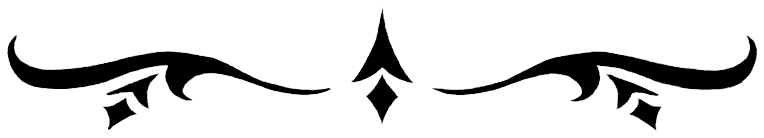
\includegraphics[width=180px]{Chronik der Andorversen/verzierung1.png}\\
        {\Huge #1} \\
        {nach andorischer Zeitrechnung}\\
        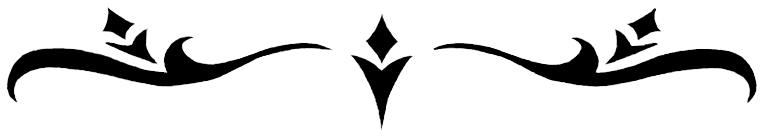
\includegraphics[width=180px]{Chronik der Andorversen/verzierung2.png}
    \end{center}
    \extramarks{}{#1 a.Z.}
}




\renewcommand{\footnoterule}{%stretche footnote-Linie über die ganze Länge
  \kern -3pt
  \hrule width \textwidth
  \kern 2pt
}

\usepackage{extramarks} %für \lastrightmark und xmark's

\renewcommand{\sectionmark}[1]{\markright{#1}} %keine Nummerierung für die section-header

\fancyhf{}%lösche alle Header-Footer-default-Einstellungen
\fancyfoot[C]{\thepage} %Seitenzahl im Footer, zentriert 
\fancyhead[L]{\nouppercase{\lastrightmark}}
\fancyhead[C]{}
\fancyhead[R]{\lastrightxmark}





\usepackage{environ}
\usepackage[most]{tcolorbox} % für farbige Boxen
\NewEnviron{chapterbox} %box für chapter-Anfänge
{   
    \newpage
    \begin{tcolorbox}[arc=0pt, colback=white, boxrule=0pt]
        \BODY
        \vfill
    \end{tcolorbox}
}

\setlength{\intextsep}{0pt}%für wrapfigure

\title{Chronik der Andorversen\\Stand Juni 2025}
\author{Werke von Michael Menzel, Stefanie Schmitt,\\Christoph Kling, Dorothea Michels, Andreas Kälber, Matthias Miller,\\Jens Baumeister, Timo Grubing, Peter Gustav Bartschat,\\Gerhard Hecht, Inka und Markus Brand, Stefan Blanck\\Alex Zbiek, Jörg Ihle, Thorsten Suckow, Julian Colbus,\\ELANE, Falke Holzapfel, Silke Lukas,\\sowie allerlei anderen andorischen Autor*innen,\\zusammengestellt von Butterbrotbär}
\date{}


\begin{document}







\hintergrund{Hintergrund.jpg}


\begin{titlepage}
    \titelseite{Grundspiel Hintergrund.jpg}
    \centering
    
    
\includegraphics[width=\textwidth]{Chronik der Andorversen/Andor Logo.png}
    \vspace{-10em}
    
    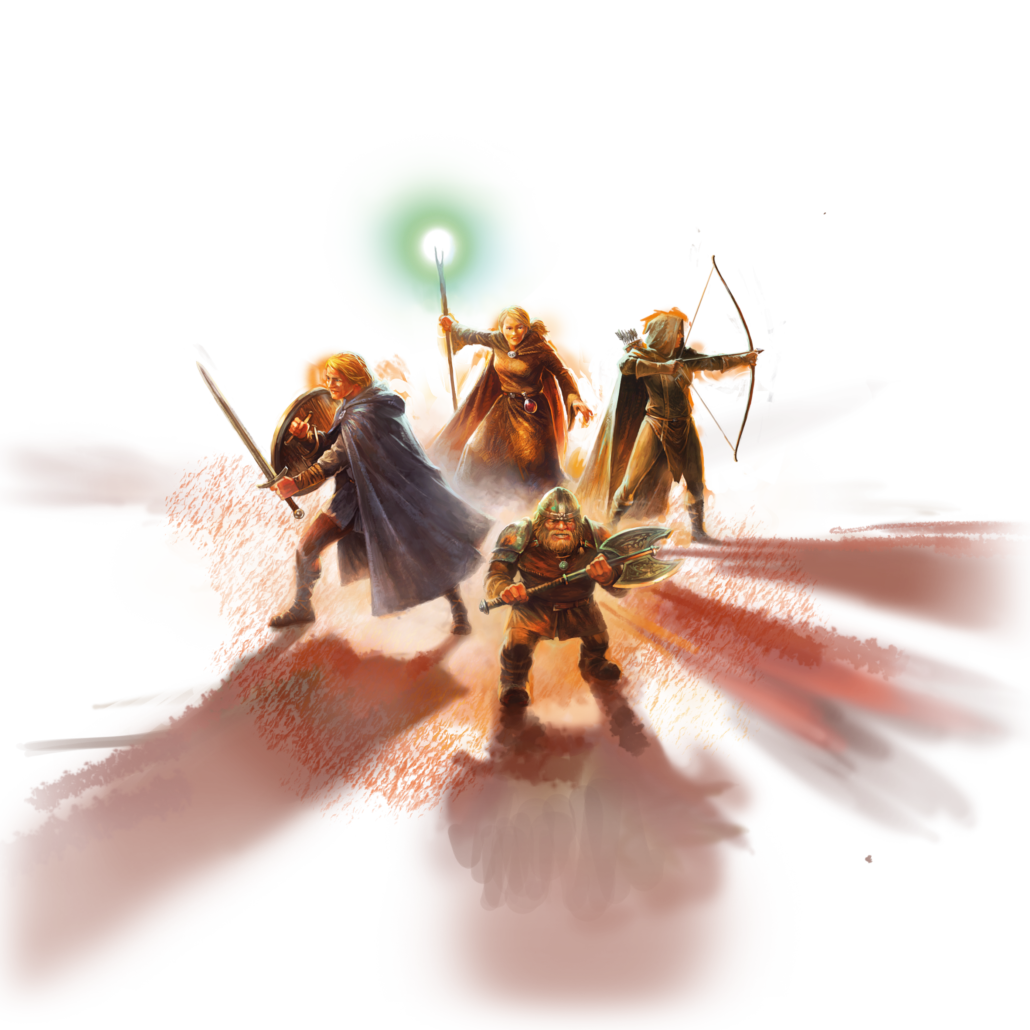
\includegraphics[width=\textwidth]{Chronik der Andorversen/Andor Helden.png}
    \vspace{-15em}

    \fontsize{72}{100}
    \textcolor{white}{\andorfont \contour{black}{Chronik der}}

    \textcolor{white}{\andorfont \contour{black}{Andorversen}}

    \fontsize{36}{50}
    \textcolor{white}{\andorfont \contour{black}{Stand Juni 2025}}
\end{titlepage}



\maketitle







\thispagestyle{plain}%keine fancy Header auf dieser Seite


\setcounter{page}{3} %lasse bereits das Titelbild als Seite 1 zählen

\textbf{Liebe Andori,}

\begin{multicols}{2}

\textbf{Die Legenden von Andor sind ein außergewöhnlich multimediales Franchise.} Nicht nur die bekannte Brettspielreihe ist dafür relevant, sondern auch zahlreiche Spin-Off-Spiele, Romane, Hörspiele, Storytexte und Alternate Reality Games. Neue und alte Andor-Fans (und sogar offizielle Autor*innen) sehen sich der nicht trivialen Frage gegenübergestellt, was es überhaupt alles an Werken zur Andor-Welt gibt, und in welcher Reihenfolge man jene erleben will.\bigskip

\textbf{Vieles zur Welt von Andor versteckt sich im Internet und verschwindet mit der Zeit.} Viele Hintergrundinformationen und -Storytexte stammen von der offiziellen Website oder aus dem offiziellen Forum, wo in Forenevents und Alternate Reality Games oft offizielle Figuren auftreten und die Geschichte Andors weitererzählen. Und so nützlich das Internet auch ist für das Zusammenbringen zahlreicher Andor-Fans aus verschiedenen Ländern, so ist auch es nicht für die Ewigkeit: Webseiten werden überarbeitet, Inhalte werden gelöscht, Links führen auf einmal ins Leere. Einige ältere Storytexte, Hörspiele und "Adventures of Hadria" sind bereits nicht mehr offiziell erreichbar. Dies wird sich im Laufe der Zeit wohl nur verschlechtern.\bigskip

\textbf{Dieses Dokument dient zweierlei Zweck. } 
Zum einen soll es eine Liste aller offiziellen Andor-Werke sein, von den bekanntesten Legenden bis zu den obskursten Spin-Offs, und diese in eine möglichst konsistente chronologische Reihenfolge bringen.
Zum anderen soll es eine Sicherheitskopie der offiziellen Andor-Texte aus dem Internet sein, schön versammelt an einem Ort.\bigskip

\textbf{Zur Zeitrechnung wird die Bonus-Box-Chronik von 2017 genutzt,} wie es der Forschungsstand zum Bannkreis von Choranat und Fan-Werke wie TroIIs "Der ewige Rat" auch tun. Produkte werden gemäß ihrem Beginn einsortiert. Icons zu allen enthaltenen Legenden unter einem Cover verlinken auf die Zeitpunkte, zu denen diese Legenden spielen. Schwer chronologisch einsortierbare Werke werden in einem eigenen Kapitel zwischen der Ära des Sternenschildes und dem Kampf um Cavern gesammelt, statt sie ganz an den Anfang oder ganz ans Ende der Chronik des Legenden-Andorversums zu stellen, da die meisten solchen Werke erstaunlich gut in diesen Zeitraum passen. Mini-Erweiterungen und Spielvarianten werden jeweils beim ersten passenden Werk aufgelistet.\bigskip

\textbf{Hier herrscht Spoiler-Gefahr für die offizielle Andor-Geschichte.} Diese Sammlung am besten geeignet für Leute, die ihren ersten Kontakt mit Andor bereits hinter sich haben. Dass die Werke hier in Andor-chronologischer Reihenfolge aufgelistet sind, soll nicht suggerieren, dass man die Produkte in dieser Reihenfolge durchspielen sollte, erst recht nicht beim ersten Erleben der Andor-Geschichte.\bigskip

\fillbreak

\textbf{Diese Sammlung kann nicht und soll nicht das Erleben der Andor-Geschichte durch die offiziellen Produkte ersetzen.} Sie enthält, von einigen wenigen Ausnahmen abgesehen, keine Inhalte aus zu kaufenden Produkten, sondern nur frei im Internet verfügbare Texte und Bilder von den offiziellen Web-Auftritten Andors. Deren Copyright liegt nicht bei mir, sondern bei Michael Menzel, dem KOSMOS-Verlag und den anderen andorischen Autor*innen. Ich wandte mich an Michael Menzel und erhielt die Erlaubnis, dieses urheberrechtlich geschützte Material in dieser Form nicht-kommerziell zu teilen. Alle anderen Rechte bleiben jedoch vorbehalten. Dieses Projekt ist ein Fan-Werk und wird nicht offiziell unterstützt.\bigskip

\textbf{Hier geht es um die Welt von Andor, nicht unsere Welt.} Im offiziellen Forum lassen sich zahlreiche Making-Ofs finden, in denen Michael Menzel und andere Autor*innen vom Entstehungsprozess hinter den Kulissen erzählen. Solche Texte sind in diesem Dokument nur enthalten, wenn sie neue Informationen zur Welt von Andor liefern. Zum Beispiel ist der Beitrag, in welchem Michael Menzel von der einst geplanten kleinen Erweiterung "Die Rietgraskrone" erzählt, hier nicht enthalten, wohl aber Auszüge zur Entstehung von Chada \& Thorn, in welchem er von Callems Hintergrund berichtet. Ebenfalls vermeide ich Fotos aus unserer Welt, erst recht von realen Personen.\bigskip

\textbf{Hier geht es um offizielle Werke, keine Fan-Werke.} Andor verfügt über eine einzigartige Fan-Community und ich bin geehrt, mich dazu zählen zu dürfen. Der Korpus an Fan-Werken widerspricht dem offiziellen Kanon aber vielerorts, und ist ohnehin viel zu groß, als dass er in ein solches Dokument passen könnte. Zum Beispiel sind Mjölnirs Fan-Legenden hier nicht aufgelistet, auch wenn Matthias Miller später als offizieller Autor Werke gestaltete. Im Zweifelsfall erwähne ich aber lieber etwas zu viel als zu wenig, weswegen hier etwa Giftknödels Erdwurm und der sagenumwobene Eismet am Rande auftauchen.\bigskip

\textbf{Werdet aktiv!} Ich werde Schreibfehler begangen, Werke vergessen und die Chronologie teilweise durcheinander gebracht haben, ganz zu schweigen davon, dass einige meiner völlig subjektiven Präferenzen in diese Sammlung geflossen sind. Bitte, gebt Rückmeldungen und Verbesserungsvorschläge (idealerweise auf \url{https://legenden-von-andor.de/forum/viewtopic.php?f=11&t=10314}), modifiziert dieses Dokument nach Lust und Laune, und eines Tages, wenn ich keine Updates mehr vornehme, zieht das Projekt weiter und erstellt selbst nächste Versionen.\bigskip

\textbf{Und nun schreitet voran, angehende Andor-Expert*innen, und verschafft euch einen Überblick über die umfangreiche Welt der Andorversen.}\bigskip

Liebe Grüße

Butterbrotbär


\fillbreak


\tableofcontents

\end{multicols}



\textcolor{white}{\part[Das Junior-Andorversum]{Das\\Junior-\\Andorversum\titelseite{Baum der Lieder Junior-Andorversum.jpg}}}




\renewcommand\thechapter{\Alph{chapter}} %damit chapters mit Großbuchstaben bezeichnet werden


\begin{multicols}{2}

\begin{chapterbox}


    \chapter{Junior-Geschichten}
    
    \begin{center}
        Beitrag aus dem offiziellen Forum

        "Der Fluch des roten Drachen - Jens Baumeister im Interview"
    \end{center}

    \textit{Gilda: Ist ein so umfangreicher Kosmos wie das Andorversum eher ein etwas enges Korsett oder eine hilfreiche Sandkiste, in der man gut spielen und der Kreativität freien Lauf lassen kann?}

    \textit{Jens: Eher eine Sandkiste. Ich bin ja mit Andor Junior in der dankbaren Situation, dass es sowieso nicht exakt dasselbe Universum sein kann wie in den "großen" Andor-Spielen: Allein die Tatsache, dass Thorn, Eara, Chada und Kram schon als Kinder zusammen Abenteuer erleben, widerspricht dem, was im "Lied des Königs" etabliert wurde. Das heißt, ich bin nicht zu 100\% an alles gebunden, was in den restlichen Andor-Produkten an (Vor-)Geschichten erzählt wurde, kann mich aber gleichzeitig aus dem großen Schatz an Ideen und Figuren bedienen, der darin bereits existiert. Aber natürlich will ich, dass es sich auch wirklich wie Andor anfühlt. Darum habe ich, wie schon erwähnt, ausgiebig recherchiert, um unnötige Widersprüche und Ungenauigkeiten zu vermeiden. Es treten viele bekannte Figuren aus dem Andorversum auf, die sich auch so verhalten, wie man es von ihnen erwarten würde; und die Schauplätze, an denen das alles stattfindet, entsprechen denjenigen, die wir vom klassischen Andor-Spielplan kennen. Wenn ich alles richtig gemacht habe, ist es hoffentlich ein neues Abenteuer in einer vertrauten Welt. Und idealerweise eines, das sowohl Kindern als auch (vorlesenden?) Erwachsenen Spaß macht.}

    \bildmitts[width=\textwidth]{Andor Junior Schlussbild.jpg}

\end{chapterbox}




\produkt{Teil 1: Der Fluch des roten Drachen (2021)}

\begin{center}
    Buch oder Hörspiel
\end{center}

\bildmitts{Der Fluch des roten Drachen (2021).png}

Der tapfere Krieger Thorn, die entschlossene Magierin Eara, die kluge Bewahrerin Chada und der clevere Zwerg Kram sind völlig unterschiedlich. Doch nur wenn sie zusammenhalten, können sie das Land Andor retten.

König Brandur ruft die Kämpfer des Landes zur Rietburg, denn im Grauen Gebirge wütet der Drache Tarok. Die Kämpfer müssen sich darauf vorbereiten, Andor zu verteidigen. Durch Zufall finden die Freunde Thorn, Eara, Chada und Kram heraus, wer hinter dem Angriff des Drachen steckt. Können sie ihn aufhalten, bevor es zu spät ist?





\produkt{Teil 2: Der Sturm auf die Rietburg (2022)}

\begin{center}
    Buch oder Hörspiel
\end{center}

\bildmitts{Der Sturm auf die Rietburg (2022).png}

Durch Zufall entdecken Thorn, Eara, Chada und Kram im Keller der Rietburg ein Skralkind, ein gefürchtetes Monster, das für den Magier Varkur spionieren soll. Doch das Skralkind will lieber Frieden stiften und möchte mit den jungen Helden Freundschaft schließen. Währenddessen versammelt Varkur eine Armee aus dunklen Gestalten und Monstern für einen erneuten Angriff. Wird es den Helden gelingen, die Rietburg zu retten?







\fillbreak
\produkt{Bücherhelden: Die geheime Botschaft (2025)}

\begin{center}
    Buch
\end{center}

\bildmitts{Die geheime Botschaft (2025).jpeg}

Viele Legenden ranken sich um das Königreich Andor und seine vier Helden Chada, Eara, Kram und Thorn. Doch auch Helden fangen einmal klein an.

Beim Trainieren in der Burg entdecken Thorn und seine Freunde einen alten Brief. Von einem Schatz ist da die Rede! Die Freunde machen sich sofort auf die Suche. Doch dann taucht der böse Magier Varkur auf. Was führt er im Schilde?





\fillbreak
\produkt{Teil 3: Das Flüstern im Wald (2023)}

\begin{center}
    Buch oder Hörspiel
\end{center}

\bildmitts{Das Flüstern im Wald (2023).png}

Die jungen Helden sollen herausfinden, wer die Felder der Bauern im Rietland verwüstet hat. Ihre Mission führt sie in den Wachsamen Wald, wo sie plötzlich einer Horde Wardraks gegenüberstehen. Schnell ist klar: Der böse Magier Varkur hat hier seine Finger im Spiel. Diesmal hat er es nicht auf die Königskrone, sondern auf Earas Kristall abgesehen, durch den er unbesiegbar werden würde. Als Thorn, Eara, Chada und Kram auch noch getrennt werden, scheint der Kampf aussichtslos und Hilfe ist nicht in Sicht ...

\end{multicols}

\hrule

\begin{multicols}{2}

\produkt{Teil 4: Die Spur aus der Vergangenheit (2024)}

\begin{center}
    Hörspiel
\end{center}

\bildmitts{Die Spur aus der Vergangenheit (2024).jpeg}

Wohin ist Aćhs Takuri verschwunden?

Festtagsvorbereitungen auf der Rietburg! Auch Ken Dorr, ein alter Weggefährte des Königs, ist zu Besuch. Plötzlich ist Aćhs Takuri verschwunden. Dahinter kann nur Garz, der Handelszwerg, stecken. Ken Dorr gibt den fünf Freunden Tipps, wie sie Turr wiederfinden können. Doch auf dem Weg zum Burgberg macht Chada eine erschreckende Entdeckung ...




\fillbreak
\produkt{Teil 5: Das Wesen im Wasser (2024)}

\begin{center}
    Hörspiel
\end{center}

\bildmitts{Das Wesen im Wasser (2024).jpeg}

Der böse Magier Varkur hat die Macht über alles Wasser von Andor errungen ...

Die Bewohner der Rietburg erreicht eine bedrohliche Nachricht: Der böse Magier Varkur hat den Mächten des Meeres einen kraftvollen Speer gestohlen. Damit hat er die Macht über alles Wasser von Andor. Tatsächlich finden die Freunde einen Brunnen, dessen Wasser untrinkbar geworden ist. Ihnen bleibt nur wenig Zeit, den Speer zurückzuholen ...




\fillbreak
\produkt{Teil 6: Die magischen Minen (2024)}

\begin{center}
    Hörspiel
\end{center}

\bildmitts{Die magischen Minen (2024).jpeg}


Tief im Berg bei den Schildzwergen treffen die Freunde auf gefährliche Zeitgenossen ...

In Cavern, wo die Schildzwerge leben, lodert ein magisches Feuer, mit dem besondere Metalle geschmiedet werden können. Doch seit einiger Zeit flackert das Feuer aus unerklärlichen Gründen. Die Freunde sind besorgt und gehen dem seltsamen Phänomen auf den Grund. Tief im Berg treffen sie auf gefährliche Lumiwürmer und monströse Maschinen ...


\fillbreak
\produkt{Teil 7: Die Dämonen im Eis (2024)}

\begin{center}
    Hörspiel
\end{center}

\bildmitts{Die Dämonen im Eis (2024).jpeg}

Die Freunde im Reich der Eisdämonen gefangen. Ein Wettlauf mit der Zeit beginnt ...

Auf der Reise nach Tulgor werden die Freunde im Reich der Eisdämonen gefangen. Siantari und Ijsdur bitten sie um Hilfe: Sie waren einst auch Kinder, doch die Dämonen haben von ihnen Besitz ergriffen. Nur mithilfe der seltenen Mera-Steine können sie in ihr altes Leben zurück – und die sind nur in dieser besonderen Nacht zu finden. Ein Wettlauf mit der Zeit beginnt ...














\begin{chapterbox}

    \chapter{Junior-Spiele}
    
    \begin{center}
        Beitrag aus dem offiziellen Forum

        "Gildas Bild der Woche, 09. März 2020: Ein erster Blick auf das Spielmaterial"
    \end{center}
    
    \textit{[Michael Menzel:] Ich bin schwer beeindruckt, wie es Inka und Markus gelungen ist, Andor als Kinderspiel umzusetzen. Besonders schön sind die variablen Aufgaben (die Karten in der Mitte), die jede Partie anders machen, da die Konstellationen immer anders sind. Statt der recht abstrakten Tagesleiste in Andor hat hier jeder Held kleine (Holz)-Sonnen auf seinem Tableau. Auch hier kostet jeder Schritt eine Stunde, aber es ist so halt viel übersichtlicher und "greifbarer" für die Kids. ;)}
    
    \textit{Mich erinnert Andor Junior sehr an die Shrek-Filme. Zwar richteten auch die sich ganz klar an Kinder - aber die Väter und Mütter, die mit im Kino saßen, hatten ebenfalls eine gute Zeit. :D}
    
    
    \bildmitts[width=\textwidth]{Andor Junior Feiern.jpeg}

\end{chapterbox}



\fillbreak
\produkt{Andor Junior (2020)}

\begin{center}
    Eigenständiges Spiel
\end{center}


\bildmitts{Andor Junior (2020).png}

Großer Schreck! Die Wolfsjungen haben sich in der Zwergenmine verirrt und brauchen dringend Hilfe. Keine Frage, dass die Helden von Andor zu ihrer Rettung eilen. Doch kaum haben sie die Rietburg verlassen, wittert der listige Drache seine Chance und macht sich zum Angriff bereit. Werden die Helden es schaffen, ihre Aufgaben zu erfüllen, bevor der Drache die ungeschützte Burg erreicht?\bigskip

\textbf{Helden:}

\begin{itemize}[topsep=0pt,itemsep=-1ex,partopsep=1ex,parsep=1ex]
    \item Chada (Pasco), die Bogenschützin 
    \item Eara (Liphardus), die Magierin 
    \item Kram (Bait), der Zwerg 
    \item Thorn (Mairen), der Krieger 
\end{itemize}


\textbf{Die Aufgaben des Brückenwächters:}

\begin{enumerate}[topsep=0pt,itemsep=-1ex,partopsep=1ex,parsep=1ex]
    \setcounter{enumi}{0}
    \item Sammelt Wolfskraut für die Wolfsjungen
    \item Helft dem verletzten Falken
    \item Die Befestigungen der Gors
    \item Das Volk Andors hungert
    \item Lieder der Hoffnung
    \item Die zerstörte Brücke
    \item Frisches Wasser für Andor
    \item Der Heiltrank der Kräuterhexe
    \item Die geheimen Briefe des Königs
    \item Der schreckliche Höhlentroll
\end{enumerate}



\fillbreak
\produkt{Die Fährtenleserin Fennah (2020)}

\begin{center}
    Erweiterung zu \refprodukt{Andor Junior (2020)}, von der offiziellen Website oder als Promo
\end{center}

\bildmitts{Andor Junior Fennah.jpeg}

\textbf{Helden:} 
\begin{itemize}[topsep=0pt,itemsep=-1ex,partopsep=1ex,parsep=1ex]
    \item Fennah (Fenn), die Fährtenleserin 
\end{itemize}



\produkt{Die Steine des Schicksals (2021)}

\begin{center}
    Erweiterung zu \refprodukt{Andor Junior (2020)}, von der offiziellen Website oder als Promo
\end{center}

\bildmitts{Die Steine des Schicksals Promo (2024).jpg}

Es steht nicht gut um Andor! In einer Vision sah Reka, die Kräuterhexe, einen unnatürlichen Sturm von ungeheurem Ausmaß heraufziehen. Er wird alles verwüsten und Unheil über das Land bringen. Doch es gibt Hoffnung. In den Tiefen der Zwergenmine versteckten einst die Ahnen einen mächtigen Runenstein, den Sonnenstein. Es heißt, er könne jeden dunklen Zauber brechen und so das Unwetter vertreiben. Aber Vorsicht! In der Mine liegen noch weitere, unheilbringende Runensteine verborgen. Werdet ihr es schaffen, den mächtigen Sonnenstein zu finden? Bevor ihr allerdings eure Suche in der Mine starten könnt, gibt es noch einiges zu tun. Mart, der alte Brückenwächter, wird die Brücke erst freigeben, wenn ihr seine Aufgaben bewältigt habt.


  
\fillbreak
\produkt{Die Gefahr aus dem Schatten (2022)}

\begin{center}
    Erweiterung zu \refprodukt{Andor Junior (2020)}
\end{center}

\bildmitts{Die Gefahr aus dem Schatten (2022).png}

Ein gefährlicher Schattenwardrak gefährdet das Wohl des Königreichs. 2-4 Spielerinnen und Spieler ab 7 Jahren brechen gemeinsam auf, um die düstere Kreatur zu verjagen. Bis es soweit ist, gibt es viele Aufgaben zu bewältigen und Gors zu bekämpfen. Die Bewohner Andors freuen sich über tatkräftige Unterstützung!\bigskip

\textbf{Helden:}
\begin{itemize}[topsep=0pt,itemsep=-1ex,partopsep=1ex,parsep=1ex]
    \item Tenaya (Teyan), die Feuerwächterin\bigskip
\end{itemize}

\textbf{Die königlichen Aufgaben:}


\begin{enumerate}[topsep=0pt,itemsep=-1ex,partopsep=1ex,parsep=1ex]
    \setcounter{enumi}{10}
    \item Eine starke Holzburg
    \item Die Leuchtfeuer brennen!
    \item Die erschöpften Helden
    \item Der kranke Hirsch
    \item Der Hornbogen
    \item Augen in der Finsternis
    \item Ein Held in Not
    \item Falkenheilung
    \item Die Gors in der Zwergenmine
    \item Rekas Nachricht
    \item Ein neuer Wachturm
    \item Neue Lieder
    \item Der brennende Wald
    \item Die Schilde des Brückenwächters
    \item Der Zwergenbrunnen
    \item Die kaputte Brücke
    \item Kraken-Alarm
    \item Kein Tropfen Wasser
    \item Händler in Gefahr
    \item Der schreckliche Waldtroll
\end{enumerate}
 

\begin{center}
    Beitrag aus dem offiziellen Forum

    "Andor Junior - Die Gefahr aus dem Schatten: Interview"
\end{center}

[...] Denn als hätten wir alle mit dem üblen Drachen schon genug Ärger am Hals, hat sich nun auch noch ein Schattenwardrak nach Andor durchgeschlagen. Und der wird stärker und stärker. Also müssen wir schnell all unsere Kräfte bündeln, um ihm zeitig den Garaus zu bereiten. Allerdings gibt es da ein klitzekleines Problemchen...naja vielleicht auch vier...fünf...sechs?

Zum einen lässt uns der Drache einfach nicht in Ruhe und flattert unentwegt in Richtung Rietburg, zum anderen stellt uns König Brandur neue, spannende Aufgaben. Andor braucht einfach an allen Ecken und Enden unsere Hilfe und solange wir nicht alles erledigt haben, was König Brandur erledigt wissen will, haben wir einfach keine Zeit, uns um den Schattenwardrak zu kümmern. Und genau deshalb ist Eile und ein kühles Köpfchen geboten!

[...] Tenaya, die Feuerwächterin kommt nicht allein nach Andor. Sie bringt Ihren treuen Begleiter, Flaps Flederfuchs, mit.

Er zeichnet sich dadurch aus, dass er unheimlich flink ist, auch in tiefster Dunkelheit nie die Orientierung verliert und an der Seite seiner Heldin tapfer für Andor kämpft. [...]

Naja, die Wolfjungen haben wir ja bereits in Sicherheit gebracht. Die toben schon lange mit ihrer Mutter an der Rietburg herum und werden zusehends größer und größer...

Von dem Schattenwardrack haben wir euch auch schon erzählt. Ihr wisst auch, dass wir uns erst um den Wardrack\footnote{BBB: Offizielle Schreibweise: Wardrak} kümmern können, wenn wir König Brandurs "To-Do-Liste" abgehakt haben...

Und wenn das dann endlich soweit ist, stürmt dieser Schattenwardrack auch schon geradewegs auf die Rietburg los.

Uns bleibt nichts anderes übrig, wir müssen uns auch diesem Wesen stellen und es bekämpfen. Je häufiger wir den Wardrack erwischen, desto schwächer wird er. Zum Glück läuft er langsamer, je schwächer er wird. Hoffen wir, ihn so noch vor der Rietburg stoppen zu können.



\end{multicols}




\textcolor{white}{\part[Das Legenden-Andorversum]{Das\\Legenden-\\Andorversum\titelseite{BdL Legenden-Andorversum.jpeg}}}

\begin{multicols}{2}
    \begin{chapterbox}
        \chapter{Landkarten}
    
        \begin{center}
            Aus \refstorytext{Die Rückkehr (2016)}:
        \end{center}
    
        \textit{[Chada] hatte mehr von der Welt gesehen als sonst ein Bewahrer. Das Land Andor, das nun weit und golden im Sonnenlicht vor ihr lag, war nur ein kleiner Ausschnitt auf der Landkarte ihres Lebens.}

        \bildmitts[width=0.75\textwidth]{Andor Landkarte LdK.jpg}
    \end{chapterbox}
\end{multicols}






\produkt{Die Karte von Andor (2012)}

\begin{center}
    Landkarte von der offiziellen Website
\end{center}

\bildmitts[width=\textwidth]{Die Karte von Andor.jpg}


\newpage
\produkt{Die Karte von Cavern (2014)}

\begin{center}
    Landkarte von der offiziellen Website
\end{center}

\bildmitts[width=\textwidth]{Die Karte von Cavern.jpg}

Diese Karte zeigt Cavern, die Mine der Schildzwerge.

Viele Legenden ranken sich um diesen Ort dessen wirkliche Größe und labyrinthische Konstruktion jeder Beschreibung trotzt.


\newpage
\produkt{Die Karte vom Land der Steppe (2023)}

\begin{center}
    Landkarte von der offiziellen Website
\end{center}

\bildmitts[width=\textwidth]{Die Karte vom Land der Steppe.jpg}


Auf ihren Abenteuern bereisten manche der Helden das Land östlich des Grauen Gebirges. Diese Karte zeigt das Land als es von der Ewigen Kälte heimgesucht wurde.


\newpage
\produkt{Die Karte des Nordens (2014)}

\begin{center}
    Landkarte von der offiziellen Website
\end{center}

\bildmitts[width=\textwidth]{Die Karte des Nordens.jpg}

Gezeichnet von Merrik, dem Kartographen, während der fantastischen Reise in den Norden an der Seite der Helden von Andor.


\newpage
\produkt{Die Karte der Insel Hadria (2015)}

\begin{center}
    Landkarte von der offiziellen Website
\end{center}

\bildmitts[width=\textwidth]{Die Karte der Insel Hadria.jpg}



\newpage
\produkt{Die Karte von Narkon (2015)}

\begin{center}
    Landkarte aus dem offiziellen Forum
\end{center}

\bildmitts[width=0.9\textwidth]{Die Karte von Narkon.jpeg}

\begin{center}
    Beitrag vom Zuckerberg
\end{center}

Nachdem die Aldebaran vom Hadrischen Meer verschlungen wurde, retteten sich im neuen 2er Spiel Chada und Thorn sowie Stinner auf die Insel Narkon. Doch wie sieht dieses unheilvolle Zipfelchen Land aus? Aus "Die Reise in den Norden" kennt ihr bereits den südlichen Teil der Insel. Für euch zur Orientierung hat Merrik, der Kartograf eine Karte erstellt. Weit ist der Weg der drei Helden in Richtung Süden...


\newpage
\produkt{Die Karte des Grauen Gebirges (2016)}

\begin{center}
    Landkarte von der offiziellen Website
\end{center}

\bildmitts[width=\textwidth]{Die Karte des Grauen Gebirges.jpg}

Diese Karte zeigt das Graue Gebirge, ein verlassenes, unwirtliches Land, das einst Heimat vieler Völker war. Heute erinnern nur noch die Bauwerke der Zwerge an jene Tage. Doch auch diese wurden größtenteils in dem Krieg zwischen Drachen, Zwergen und Trollen vernichtet, ein Krieg, der mit dem Schmieden des letzten der vier mächtigen Schilde begann: Dem Feuerschild!

\newpage
\produkt{Die Karte des Landes Krahd (2017)}

\begin{center}
    Landkarte von der offiziellen Website
\end{center}

\bildmitts[width=\textwidth]{Die Karte des Landes Krahd.jpg}

Krahd war wie ein verzerrtes Abbild Andors. Selbst die Orte, wie die Feste von Borghorn, der Schwarze Baum oder die Wurfmaschine, lagen wie spiegelverkehrt gegenüber der Rietburg, dem Baum der Lieder oder dem Alten Wehrturm. Doch Andor stand für die Freiheit, Krahd für die Unterdrückung.

\begin{center}
    Beitrag aus dem offiziellen Forum
\end{center}

PS: Gezeichnet wurde die Karte übrigens von Merrik, dem Kartographen.


\newpage














\begin{multicols}{2}

\begin{chapterbox}

    \chapter{Der unterirdische Krieg}
    
    
    
    \begin{center}
        Aus \refprodukt{Die Karte des Grauen Gebirges (2016)}:
    \end{center}
    
    \textit{[D]as Graue Gebirge, ein verlassenes, unwirtliches Land, das einst Heimat vieler Völker war. Heute erinnern nur noch die Bauwerke der Zwerge an jene Tage. Doch auch diese wurden größtenteils in dem Krieg zwischen Drachen, Zwergen und Trollen vernichtet, ein Krieg, der mit dem Schmieden des letzten der vier mächtigen Schilde begann: Dem Feuerschild!}\bigskip
    
    \bildmitts[width=\textwidth]{Kreatok und Nehal.jpeg}
    
    
    [Die Geschichten darüber, wie die junge Sian zur Eisdämonin Siantari und die junge Rosanna zur Schattenhexe Shan werden, spielen ebenfalls Jahrhunderte vor den Legenden von Andor. In dieser Sammlung findet ihr sie jedoch später, unter \refstorytext{Siantari (2018)} und \refstorytext{Schatten und Verzweiflung (2020)}.]

\end{chapterbox}





    

\fillbreak
\storytext{Der Sternenschild (2012)}

\begin{center}
    Storytext von der offiziellen Website
\end{center}

\bildmitts{Der Sternenschild Bild 1.jpg}

Der Sternenschild stammt aus einer Zeit als noch keine Feindschaft zwischen Schildzwergen und Drachen war. Einst, ehe Krahall\footnote{BBB: Moderne Schreibweise: Krahal}, der Ort der den Drachen Leben spendet, erschüttert wurde, bestand ein Bündnis zwischen Drachen und dem Volk der Zwerge. Es bestand darin, dass die Zwerge tief unter der Erde Schächte und riesige Hallen gruben, die den Drachen als Heimstatt dienten. Im Gegenzug übergaben die Drachen den Zwergen die Geheimnisse des Feuers und erlaubten ihnen damit, die ewige Düsternis unter dem Gebirge zu vertreiben. Doch eines Tages begannen die Zwerge dem Feuer neue Wunder abzuringen. Zuerst begannen sie schöne Gefäße und Lampen zu schmieden und später Ketten und Ringe als Einfassungen für die Edelsteine der Tiefe. Dann erdachten sie stählerne Tore für ihre Schatzkammern und Zorn überkam die Drachen. Als die Zwerge Waffen schmiedeten, scharf wie Drachenklauen und Rüstungen hart wie Drachenschuppen, loderte die Wut der Drachen auf und der Bund zerbrach. Ein unterirdischer Krieg entbrannte.\bigskip

Der Legende nach gab es, bevor sich Wut und Zorn in das Bündnis schlichen eine besondere Zeit. Sie war nur von kurzer Dauer, aber veränderte Vieles. Kreatok, der Zwerg war ein begabter Schmied, ausgestattet mit sehr viel Neugier und Wissensdurst. Ihm zur Seite stand Nehal, ein junger Drache, temperamentvoll und stark, aber auch gewillt etwas Neues zu erschaffen. Durch das Geschick des Zwergs und dem Feuer des Drachen entstanden vier mächtige Schilde.\bigskip

Einer dieser Schilde war der Sternenschild. Er verlieh seinem Träger Hoffnung, auch wenn die Situation ausweglos erschien.\bigskip

Autorin: Stefanie Schmitt





\fillbreak
\storytext{Der Bruderschild (2014)}

\begin{center}
    Storytext von der offiziellen Website oder aus dem offiziellen Forum
\end{center}

\bildmitts{Der Bruderschild Bild 1.jpg}

Der Bruderschild war einer der vier mächtigen Schilde aus alter Zeit. Als Zwerge und Drachen noch in Freundschaft verbunden waren, schufen Kreatok, der Zwerg und Nehal, der Drache diesen Schild. Der Legende nach besaß er die Macht, die Kraft des einen Waffenbruders auf einen anderen übergehen zu lassen. Dies war eine mächtige Waffe, denn die Zwergenminen von Cavern waren groß. Die weiten Entfernungen wurden zum Problem, denn auch die besten Kämpfer konnten nicht überall gleichzeitig sein.

In den Wirren der Zeit, ging auch dieser Schild verloren und blieb lange Zeit unerkannt. Sein schlichtes Aussehen verriet seine Stärke nicht, nur wer die feinen Hand-Ornamente auf dem Schildbuckel erkannte, wusste, um welch mächtigen Schild es sich handelte.\footnote{Diesen Abschnitt gibt es nur in der Version im offiziellen Forum.}

Als die Helden von Andor um weitere Kämpfer verstärkt wurden, wie den Taren Bragor oder Kheela, der Hüterin der Flusslande, wurde auch dieser Schild gefunden und war den Helden von großem Nutzen.\footnote{Diesen Abschnitt gibt es nur in der Version von der offiziellen Website.}\bigskip

Autorin: Stefanie Schmitt



\fillbreak
\storytext{Zum Silberschild}

\begin{center}
    Aus \refstorytext{Der Sturmschild (2014)}:
\end{center}

Als Hallwort an jenem eingangs erwähnten Morgen in die Waffenkammer ging und das feingearbeitete Kettenhemd, den goldenen Brustpanzer angelegt und den großen kantigen Helm aufgesetzt hatte, fiel sein Blick auf einen Schild in der Ecke. Der Fürst nahm ihn auf und betrachtete die reichen Verzierungen und dachte an Nehal, den Drachen und Kreatok, den Meisterschmied der Schildzwerge, die einst gemeinsam der Schmiedekunst nachgingen und die vier mächtigen Schilde erschufen. Dies hier war der Silberschild und der Fürst lachte. "Dieses nutzlose Ding! Ha, ha."\bigskip

Tatsächlich war dieser Schild für alle Zwerge eine Enttäuschung gewesen. Zuvor hatten Nehal und Kreatok den Sternenschild gefertigt, einen der  bedeutendsten der vier. Dieser vermochte Böse Geschehnisse aufzuhalten  und das Schicksal zum Guten zu wenden. Kurz darauf entstand der Bruderschild, ein ebenfalls machtvoller Schild.  Dieser erlaubte es seinem Träger, die Kräfte eines anderen Zwerges anzunehmen oder die eigenen einem anderen Bruder zu übertragen. So konnten die Zwerge auch über weite Entfernungen einander schützen.\bigskip

Nachdem diese beiden wunderbaren Schilde entstanden waren, war die Erwartung bei den Schildzwergen groß. Was würde der nächste Schild bewirken, der Nehals glühender Esse und Kreatoks Amboss entsprang? Welchen Schutz würde er wirken? Feinstes Silber und Gold wurden den beiden für ihre nächsten Werke überlassen. Und schon bald hatten sie einen weiteren Schild gefertigt.

Er war leicht und herrlich verziert. Der Fackelschein der großen Halle ließ ihn silbern aufleuchten, als die Zwerge ihn das erste Mal sahen. Doch wie sich bald herausstellte, besaß dieser Schild keinerlei besondere Wirkkraft. Viele vermuteten schon Kreatok und Nehal hätten ihre Kräfte in der Schmiedekunst eingebüßt.\bigskip

Doch diese Sorgen erwiesen sich schon bald als unbegründet, denn der Meisterschmied und der Drache fertigten einen weiteren und letzten Schild. Seine Fähigkeiten ließen alle Zweifel verblassen. Ob der bald darauf folgende Krieg zwischen Zwegen und Drachen auch seinetwegen entflammte, ist ungewiss, doch keineswegs unwahrscheinlich.

Jedenfalls lobten alle Zwerge das Geschick Kreatoks und Nehals und der eine Schild, der keine Fähigkeiten offenbarte, wurde daraufhin als Ausrutscher abgetan und schon bald fast vergessen. Erinnerte sich ein Zwerg an ihn, so wurde er manchmal der Silberschild, manchmal der stille Schild aber meistens der Nutzlose Schild genannt.\bigskip

Und so mag es wenig verwundern, dass lange Zeit danach, als die anderen Schilde bereits in den Kriegen gegen Drachen und Kreaturen verloren gegangen waren, der nutzlose Silberschild noch immer im Besitz des Fürsten von Cavern war.




\fillbreak
\storytext{Der letzte der vier Schilde (2016)}

\begin{center}
    Inoffizielle Abschrift eines Hörspiels aus dem Abenteuer Andor Blog
\end{center}

\bildmitts{Kreatok und Nehal.jpeg}

Wie die meisten von euch wissen, wurden die mächtigen vier Schilde vor Urzeiten von dem äußerst geschickten Schildzwerg Kreatok und dem jungen Drachen Nehal geschmiedet. Es waren Nehals Drachenfeuer und Kreatoks Kunstfertigkeit, die solche Wunder entstehen ließen. Natürlich mag es in heutiger Zeit seltsam anmuten, dass ein Zwerg und ein Drache gemeinsame Sache machten. Doch beide Völker waren in jener Zeit, wenn auch nicht befreundet, so doch zumindest im Bunde. Anderen Völkern, wie Riesen, Trollen und Erdgeistern, standen beide weniger wohl gesonnen gegenüber.

Die Schilde erregten viel Aufsehen. Der Sternenschild, der Bruderschild, der Sturmschild und zu guter Letzt der ... manche nannten ihn den Dunkelschild, weil er das wohl dunkelste Kapitel der Schildzwerge eröffnete. Aber als Kreatok und Nehal ihn schufen, tauften sie ihn den Feuerschild. Neugierig und erwartungsvoll kamen die Zwerge und auch manch ein Drache, um die Fertigstellung dieses neuen Wunderwerks zu begutachten. 

Der Schild war schwarz, matt schimmernd wie Samt und mit wenigen Ornamenten an den Rändern. Kreatok legte den Schild an und plötzlich breiteten sich Flammen um ihn aus. Nicht rot, sondern schwarz und silbrig. Nehal, der Drache, schrie auf, denn das Feuer breitete sich rasch aus und versengte seine Flügel. Wie konnte das geschehen? Nichts konnte einen Drachen verbrennen, nichts brannte heißer als Drachenfeuer. Nehal floh vor seinem alten Freund, der ihn offensichtlich betrogen hatte. Auch die Zwerge stürmten schreiend aus der alten Felsenhalle. Doch manch gescheiterer unter ihnen begann zu jubeln. Denn jene hatten erkannt, dass dieser Schild eine unglaubliche Waffe war. "Schwarzes Feuer!", rief einer von ihnen hysterisch. Dann, verschanzt in einem Türeingang betrachteten sie das Feuer gierig und fasziniert. In dessen Mitte stand Kreatok, lachend und singend. Denn ihm allein schienen die Flammen nichts anhaben zu können. Der Schild in seiner Hand schützte ihn. Die wenigen Drachen, die anwesend waren und das Schauspiel erschreckt verfolgt hatten, wollten ebenfalls fliehen. Doch nur einer von ihnen entkam den Flammen und floh in einen langen Gang. Es war der schlauchartige Gang, den die Zwerge Barathrum nannten, die Lunge von Cavern. 

Der Drache schraubte sich in Spiralen in Barathrum empor. Gleichzeitig drang er mit seinem Geist in Krahal ein, den magischen Ort, an dem das Bewusstsein aller Drachen liegt. "Verrat!", schrie er und berichtete, dass der letzte Schild der Zwerge nichts anderes als eine Kriegserklärung an alle Drachen war. Die Drachen horchten auf und im Kollektiv ihrer Gedanken mischte sich Zorn und Furcht vor diesem schwarzen Feuer der Zwerge. Der junge Drache selbst forderte seine Artgenossen zum schnellen Vernichtungsschlag gegen die Schildzwerge auf, ehe sie mehr dieser gefährlichen Waffen erschaffen würden, und die Drachen stimmten zu.

So entflammte der unterirdische Krieg zwischen Schildzwergen und Drachen, in dem beide Völker nahezu ausgelöscht wurden. Dieser Krieg wurde nie beendet. Erschöpfung der Kräfte auf beiden Seiten führten zum Stillstand, in dem die Schildzwerge sich langsam erholten. Die letzten Drachen allerdings starben oder versteinerten mit den Jahren. Nur bei einem von ihnen, dem jungen Drachen, der die Kraft des Feuerschildes mit eigenen Augen gesehen hatte, erlosch die Flamme des Zorns nie. Er wuchs in den Jahren des Krieges und wurde mächtiger denn je. Fast so, als ginge die Kraft aller Drachen in diesen einen über. Sein Name war Tarok.



\newpage % damit eine Fußnote auf der richtigen Seite steht

\storytext{Die Winterburg (2016)}

\begin{center}
    Storytext von der offiziellen Website
\end{center}

\bildmitts{Die Winterburg (2016).jpeg}

\textbf{Prolog:}\footnote{BBB: Dieser Prolog spielt Jahrhunderte später, direkt vor \refprodukt{Die letzte Hoffnung (2016)}.} Unsere Helden waren in das verwüstete Andor zurückgekehrt und beschlossen die Verfolgung der Krahder aufzunehmen. Sie wollten die verschleppten Andori nicht der Folter der Sklaverei überlassen. Ihr Weg führte durch das graue Gebirge. Früher ein Ort, an dem Zwergenfürsten, Riesen und Drachen lebten und in späterer Zeit Kriege gegeneinander führten. Ein geschichtsträchtiges Niemandsland, über das wenig bekannt und über das selbst im Baum der Lieder kaum etwas zu finden ist. Die Geschichte der Winterburg allerdings wird dort aufbewahrt, und auch wenn keiner unserer Helden sie je las, so sollt ihr sie nun hören...

\bildmitts{Die Winterburg Bild 1.jpg}

Einst, als es noch große Zwergenreiche im Grauen Gebirge gab, bauten diese nicht nur unterirdische Tunnel und Hallen. Hier und da schlugen sie überirdische Türme und Festungen aus dem Fels. Dabei waren sie stets bemüht im Einklang mit den natürlichen Felsformationen zu sein, wie zu Stein gewordene Echos der Natur. Mächtige Statuen von Drachen und Zwergen erschufen sie, die noch immer wie stumme Wächter aus dem Nebel ragen.\bigskip

Die schönste und größte Festung war die Burg Karulzar. Erbaut auf einem so hohen Grat, dass sie häufig noch lange in den Sommer hinein Schneehauben auf ihren Türmchen trug. So wurde sie allen bald als die Winterburg bekannt.\bigskip

In ihrer langen Geschichte hatte sie viele Besitzer. Zuerst waren da natürlich die Zwerge. Doch in den Kriegen gegen die Drachen und Riesen verließen sie ihre überirdischen Festungen und zogen sich in die unterirdischen Hallen zurück.\bigskip

Drachen ließen sich bald darauf in den geräumigen Türmen und Sälen nieder. Jedoch nur für kurze Zeit, denn die Riesen hatten ein Auge auf die Festung geworfen. Sie war schön und stark. Die Riesen wussten um die Kunstfertigkeit der Zwerge und die Qualität ihrer Erzeugnisse zu schätzen, obgleich sie die Zwerge selbst verbascheuten.\bigskip

Aber der eigentliche Grund für ihr Interesse an der Winterburg war, dass sie zu nah an den Grenzen ihres eigenen Landes war, als das man sie einem Feind wie den Drachen überlassen wollte. Die Drachen jener Zeit waren weise und mächtig und den Riesen weit überlegen. Ein gefährlicher Nachbar.\bigskip

Doch gab es einen unter den Riesen, den selbst die Drachen fürchteten, denn er war ein Hexer. Nomion nannte er sich. Er war der erste Riese, der die Hexerei erforschte und ihre Macht über andere entdeckte. Seine Fähigkeiten nahmen rasch zu und bald schon konnte er Tränke für die Riesenkrieger brauen, die ihren Willen stärkten. Er entwickelte die Gabe, anderen Wesen seinen Willen aufzuzwingen und sie zu beherrschen. Und als es ihm gelang die toten Gebeine gefallener Riesen wieder auferstehen zu lassen, hatte seine Hexerei das Leben seines Volkes völlig verändert. Sie nannten sich fortan die Krahder, die Unsterblichen. Dies war natürlich Unsinn, denn sie starben wie alle anderen Wesen auch, wenn ihre Zeit gekommen war. Und das was die Toten wiederauferstehen ließ war die Macht Nomions. Und doch war es die Hexer, die sie von anderen Riesen unterschied und sie zu Krahdern machte.\bigskip

Und Nomion gab sein Wissen weiter und seine Schüler errichteten Tempel und pflanzten den Schwarzen Baum um die böse Hexerei zu nähren und allgegenwärtig zu machen, wie die Luft zum Atmen.\bigskip

Nomion aber strebte nach mehr. Er suchte sich im Gauen Gebirge einen verlassenen Turm der Zwerge und hielt lange Ausschau nach dem wohl mächtigsten Wesen der ganzen südlichen Welt. Und als er es fand versklavte er dessen Geist und machte es sich zum Untertan.\bigskip

Bald schon ließ er es die Winterburg angreifen. Viele junge Drachen fanden den Tod bei dieser schrecklichen Attacke und die stolze Feste von einst barst unter den Schlägen des unglaublichen Wesens.\bigskip

Doch fand an diesem Tag auch Nomion sein Ende. Der stärkste und gerissenste aller Drachen, Tarok, fand den Hexer, der unweit des Geschehens im Verborgenen seine Kreatur befehligte. Nomion war kein großer Kämpfer und sein mächtiger Diener war im Kampf gegen die Drachen auf der Winterburg verstrickt. Tarok hatte keine Mühe Nomion zu vernichten und es blieb nur ein Haufen Asche von dem Hexer zurück.\bigskip

Das Wesen, das man später den Urtroll nannte, ließ bald darauf von der Winterburg ab und zog sich zurück in seinen steinernen Schlaf. Kaum ein Drache hatte den Angriff überlebt und die Feste war zerstört.\bigskip

Die wenigen überlebenden Drachen verließen die Winterburg, die nun nicht mehr Schutz bot als irgendein Fels. Doch sollte die Ruine nicht lange unbewohnt bleiben. In der grauen Asche, die einst Nomion gewesen war, regte sich etwas. Ein bläuliches Glühen flammte auf, als sich eine blasse Gestalt erhob. Lange noch sollte diese die verlassenen Festen und Türme des Graue Gebirges heimsuchen. Es war Nomions Geist.\bigskip

Wird sein Geist noch immer dort sein, wenn ihr euch im Herbst auf den Weg ins Graue Gebirge macht ...?    \bigskip  

Autor: Stefanie Schmitt und Michael Menzel

Zeichnung: Johannes Schmitt



\fillbreak
\storytext{Die Kreaturen (2012)}

\begin{center}
    Storytext von der offiziellen Website\footnote{Die Version von der offiziellen englischen Website unterscheidet sich teils von der deutschen. Hier wurden \textit{kursiv} einige frei übersetzte Textstellen von dort ergänzt.}
\end{center}

\bildmitts{Die Kreaturen Bild 1.jpg}

\textbf{Tarok und die Kreaturen}

Krahal, der magische Ort der den Drachen Kraft und Energie verlieh, wurde vor vielen Hundert Jahren tief erschüttert. Die Drachen starben und nur einer von ihnen überlebte. \textit{Sein Name war Tarok, ein enormer Drache mit schwarzen Flügeln.} Aus den Tiefen von Krahal krochen Geschöpfe, unsagbare Kreaturen mit zerstörerischen Kräften. Irgendwann verließen sie Krahal und scharrten sich in den Bergen und Wäldern von Andor, um für den letzten Drachen zu kämpfen und zu töten.\bigskip

Es waren Gors, bösartige Geschöpfe vor denen sich Menschen und Zwerge gleichermaßen fürchteten. \textit{Sie hatten keinen Namen, als sie in Andor ankamen, doch die Bewahrer vom Baum der Lieder nannten sie }"\textit{Gors.}" Ihre Arme und Beine waren mit Schuppen übersät. Ihre Hände waren zwei riesige, spitze und scharfe Hornklauen. Gebeugt und unterwürfig war ihre Haltung und sie schienen ohne Verstand auf Befehle der Drachen zu warten.\bigskip

Es gab noch weitere Geschöpfe, Skrale und Wardraks. Skrale waren sehr groß und muskulös \textit{mit gefährlichen Drachenschwänzen}. Sie trugen riesige Schwerter in den Händen. An Armen und Beinen wurden ihre Körper durch Rüstungsteile bedeckt, um sie im Kampf zu schützen. Sie waren gefährlich, denn sie trafen eigene Entscheidungen und konnten mit Verstand einen Kampf gewinnen. Echsengleich, groß und schnell waren die Wardraks. Ihre Augen glühten wie Kohlen, bösartig und gemein. \textit{Die Wardraks waren noch größer und stärker als Skrale, und ihre schwarze Haut tarnte sie gut in der Nacht, wenn sie sich schnell in Richtung der Rietburg bewegten.} Sie waren pfeilschnell und konnten an den spitzesten Felsen emporspringen und mit ihren scharfen Krallen töten, was ihnen in die Quere kam.\bigskip

Ihr Herr, der Drache der überlebt hatte, hieß Tarok. Ein riesiges Geschöpf. Monströse, messerscharfe Schuppen bedeckten den gigantischen Körper. Riesenhafte Flügel ragten aus dem Rupf und der Kopf saß auf einem schlangenartigen Hals. Blutrot und gemein blickten seine Augen.\newpage % damit eine Fußnote auf der richtigen Seite steht
Es gab niemanden der Tarok nicht fürchtete und seit Jahrhunderten befand er sich im Grauen Gebirge und machte ein Durchschreiten der Berge unmöglich. Brandur aber stellte sich dem Drachen entgegen. Seine Willenskraft und Entschlossenheit ließen den Drachen um sein unsterbliches Leben fürchten. Er ließ Brandur und seine Freunde passieren und sendete seither seine Kreaturen aus, um ihn zu töten. Jahre später, als Tarok die Rietburg Angriff waren es nur noch die Helden von Andor, die sich ihm entgegenstellten.\bigskip

Autorin: Stefanie Schmitt






\storytext{Die Trolle (2012)}

\begin{center}
    Storytext von der offiziellen Website\footnote{Die Version von der offiziellen englischen Website unterscheidet sich teils von der deutschen. Hier wurden \textit{kursiv} einige frei übersetzte Textstellen von dort ergänzt.}
\end{center}

\bildmitts{Die Trolle Bild 1.jpg}

Die Trolle lebten schon immer in Andor. Sie waren riesenhafte und einfältige Geschöpfe, die über eine enorme Kraft verfügten. Sie töteten willkürlich und quälten Mensch und Tier. Lange bevor Brandur und seine Freunde Andor erreichten, lieferten sich die Bewahrer des wachsamen Waldes und die Trolle unerbittliche Kämpfe.

Arme und Beine der Trolle bestanden aus riesigen Muskeln und ihr Oberkörper schien alles andere zu überragen. Waffen trugen sie nicht bei sich, sondern nahmen im Kampf, was ihnen groß genug erschien, Baumstämme oder Felsen. Kleinere Gegenstände konnten sie mit ihren riesigen Pranken nicht greifen. Auch sie beeinflussten das Schicksal von Andor. Zwanzig Jahre bevor das Spiel "Die Legenden von Andor" beginnt findet die letzte große Schlacht am Sommerfels statt. \textit{König Brandur, in einem Bündnis mit den Bewahrern, hatte Erfolg.} Diese Schlacht beendete die Trollkriege und seither gibt es nur noch sehr wenige von ihnen. \textit{Viele Jahre lang dachten die Andori, kein Troll hätte überlebt. Sie lagen falsch.}\bigskip

Autorin: Stefanie Schmitt




\fillbreak
\storytext{Das Volk der Krahder (2016)}

\begin{center}
    Beiträge aus dem offiziellen Forum

    "Gildas Bild der Woche, Das Volk der Krahder"
\end{center}

\bildmitts{Das Volk der Krahder}

Dieses Riesen-Volk lebt weit im Süden in dem Land Krahd. Sie halten sich Menschen und Zwerge als Sklaven und niemand entkommt. Nun, fast niemand ...

\begin{center}
    "Andor III: Lob und Kritik"
\end{center}

%\bildlinks[width=0.1\textwidth]{Profil Michael Menzel.jpg}

[Michael Menzel:] [...] die Krahder sind tatsächlich ein sehr kleines, grässliches und inzestuöses Volk. Sicher mehr als die 4 im Spiel, aber eben nicht viele. Darum brauchen sie Sklaven, die für sie schuften und die Drecksarbeit erledigen. Ihre Armeen bestehen aus Skeletten. Selbst Trolle unterwerfen sie und richten sie zu Wachtrollen ab oder nutzen sie für andere Tätigkeiten. Nomion, ebenfalls ein Krahder, hatte sich sogar den Urtroll zum Untertan gemacht.




\begin{chapterbox}
    \chapter{Der Flammensohn}
    
    \begin{center}
        Aus \refstorytext{Die Zwei Orden (2014)}:
    \end{center}
    
    \textit{Orweyn selbst war wissbegierig, aber kein kampferfahrener Krieger. Doch eines Tages sollte ihm das Schicksal diesen Krieger bringen. Ein großes Schiff erreichte die Küste von Hadria. Es war die Tambur und ihr Kapitän war der stolze Meereskönig Varatan. [...] Dieser Meereskönig, dessen Name so viel bedeutete wie Flammensohn, schien genau der Richtige für seine Pläne zu sein.}
    
    \bildmitts[width=\textwidth]{Varatan.jpg}    
\end{chapterbox}




\fillbreak
\storytext{Die Geschichte von Danwar (2019)}

\begin{center}
    Storytext aus dem offiziellen Forum
\end{center}

"Es sieht aus als hätte man einen verdammten Arrog versteinert", soll einstmals der berühmte Seekrieger Ruuf gesagt haben, als er an Bord seines Kriegsschiff die Insel Danwar zum ersten Mal erblickte. Andere erinnerte das Bergmassiv an eine erstarrte Sturmflut.

\bildmitts{Die Geschichte von Danwar (2019).jpg}

Tatsächlich handelte es sich bei der Insel Danwar, um Lavagestein und im Kern, brodelte es noch immer, weshalb die ganze Insel Wärme abstrahlte. Wellen verdampften, wenn sie gegen das Bergmassiv schlugen. Wann immer sich ein Schiff hierher verirrte, stellte dessen Besatzung meist rasch fest, dass die Strömung unterhalb des Felsens nachließ und eine Art ruhiges Bassin bildete. Dort ankerten die Schiffe, während Personen und Ladung mit Flaschenzügen hoch zum Plateau der Insel gezogen wurden.\bigskip

Die Menschen Danwars hatten sich mit ihrer Umgebung so gut zurechtgefunden, wie es eben ging. Fremde wurden herzlich willkommen geheißen, denn der Durst nach Wissen, nach Neuem und nach Fortschritt war groß. Doch blieben nur wenige Fremde länger als nötig auf diesem unwirtlichen Flecken. Nach deren Abreise versuchten sich die Danware an alle Einzelheiten zu erinnern und das Gehörte zu archivieren.\bigskip

Weil sich auch hin und wieder Zauberer aus Hadria und Taren aus Sturmtal hierher begaben, erfuhren sie so manches über die Kräfte der Kräuter und die Macht der Zauberei. Wenn sie dann wieder unter sich zurückblieben, versuchten sie das Gelernte zu imitieren. Auf diese Weise entwickelten sie beachtliche Fähigkeiten im Umgang mit Feuer und Wasser. Beide Elemente spielten eine große Rolle auf Danwar. Sie zu beherrschen und für sich nutzbar zu machen, wurde zu einer wichtigen Aufgabe, denn Danwars Lage veränderte sich, als durch Zufall der erste Lavastein gefunden wurde. Feuerrot und massiv wie ein Rubin, schien er gleichwohl die Kühle und sogar das Geräusch des brandenden Meeres in sich zu bergen.

Als sich die Kunde über diese sagenhaften Steine verbreitete, weckte diese bis dahin unwichtige Insel, größtes Interesse. Bald kam es zu Überfällen auf Danwar und wenig später tauchten erste Kriegsschiffe aus Klippenwacht auf. Etwas so Verlockendes wie die Lavasteine, war viel zu wertvoll, um es den einfältigen Inselbewohnern zu lassen.\bigskip

Die Lage war ernst! Selbst wenn die Danware ihrer friedlichen Natur folgend, die Lavasteine freiwillig abgegeben hätten, so hätte ein massiver Abbau der Steine gleichzeitig die Stabilität der gesamten Insel bedroht. Die Danware mussten sich gegen die Angreifer verteidigen. Dies war die Geburtsstunde der Wassermagier und Feuerkrieger. Bis heute sind sie die Beschützer ihrer Insel.\bigskip

Die Danware blieben fortan unter sich, stets in Alarmbereitschaft und nie verließ ein Feuerkrieger oder Wassermagier die Insel.\bigskip

\textbf{Nie?} Nun, wie es scheint haben ein Wassermagier und ein Feuerkrieger doch den Weg nach Andor gefunden ... :D :D :D\bigskip

Hier geht es zu unserem Fan-Wettbewerb 2019: 

[Link auf \refprodukt{Feuer und Wasser (2019)}]\bigskip

\begin{center}
    Beiträge aus dem offiziellen Forum
\end{center}

[Boggart:] Könnte man die Insel als einen Baum der Lieder des Nordens bezeichenen?

[Michael Menzel:]@ Boggart: Ich glaube eher nicht. Die Bewahrer am Baum der Lieder sind ja schon sehr "weise". Ich denke die Danware wollten einfach nur das bisschen Wissen nicht sofort wieder verlieren. Aber wie bei "Stille Post" wurde aus dem Gelernten etwas völlig anderes. Vielleicht sind die Zauberer Hadrias im Nachhinein sogar ein bisschen überrascht, wie gut die Wassermagier und Feuerkrieger die Elemente im Griff haben.




\fillbreak
\storytext{Varatans Fluch (2015)}

\begin{center}
    Storytext von der offiziellen Website
\end{center}

"Pah, Seemannsgarn!", sagte König Varatan stets, wenn ihm jemand von den drei Mächten des Meeres berichtete. Er sagte dies, bis zu dem Tag, an dem er auf die gefährlichste von ihnen stieß: Kenvilar, die Tückische.

Mochte der mächtige Oktohan auch ein Schiff mit seinen Tentakeln zum Bersten bringen und Arkteron gefürchtete Stürme entfachen, Kenvilar war die verhängnisvollste  von ihnen. Ihre Tücke paarte sich mit grausamer Weisheit.\bigskip

Als diese eines Tages dem Schiff des Königs auflauerte und mehrere Seeleute in die Tiefe zog, fiel ihr ein Varatanier am Ruder des Zweimasters auf. Groß und kräftig stand er da. Die Mannschaft versuchte mit Harpunen und Seeschwertern der Gefahr Herr zu werden, aber Kenvilar beachtete sie kaum.

Sie fasste den jungen Steuermann ins Auge, sah in seine Zukunft, sah sein Potential und die schlafende Bosheit in ihm. Kevilar spürte, dass sie mit ein weing Geduld viel mehr Schaden anrichten konnte. Und so zog sie sich zurück.\bigskip

Der König feierte seinen vermeintlichen Sieg über eine der drei Mächte des Meeres mit allem was dazugehörte. Die Überlebenden wurden geehrt und der Toten wurde gedacht. Wein wurde getrunken und üppig gespeist. Das Fest blieb noch lange in Erinnerung.

Es vergingen Jahre, ehe sich die Wege des Steuermanns und Kenvilars erneut kreuzten.  Der Name des Mannes war Callem. Er hatte mittlerweile das Kommando über ein eigenes Schiff erhalten und segelte zwischen Varatanien oder Werftheim, wie es später genannt wurde, und Klippenwacht, der Seefeste König Varatans.\bigskip

Auf einer dieser Fahrten verließ er ohne ersichtlichen Grund seine Route und befand sich bald schon in stürmischen Gewässern wieder. Dort tauchte Kenvilar auf und der einstige Steuermann geriet in ihren Bann ...\bigskip

Das Schiff und seine Mannschaft galten bald als verloren und wurden mit allen erdenklichen Ehren betrauert. Callem, ihr Kapitän, war ein bekannter Seekrieger gewesen und sein Tod bedeutete einen schweren Verlust für den König.\bigskip

Es war jene Zeit, in der Varatan zu grübeln begann, wie man den Mächten des Meeres Herr werden könnte. Wenig später würde ihn sein Weg nach Norden führen, nach Hadria in das Land der Zauberei, wo er mit Orweyn, dem mächtigsten Zauberer, die magischen Waffen entwickeln sollte.\bigskip

Doch ehe all dies geschah, gingen Gerüchte über ein schwarzes Schiff um. Es tauchte aus dem Nichts auf und verschwand auf die gleiche Weise! Handelsschiffe wurden überfallen und ihrer Waren beraubt. Mal hier und mal dort wurde das schwarze Schiff gesichtet und seine Besatzung ...  sie war das Seltsamste, denn an Bord befanden sich nicht nur einfache Seeleute und abtrünnige Seekrieger. Unter ihnen waren auch Hexer und Zauberer, Druiden und andere machtvolle Wesen. Darum gelang es lange Zeit nicht an die schwarze Kogge, wie das Schiff nun allerorts genannt wurde, heranzukommen.

\bildmitts{Varatans Fluch Bild 1.jpg}

Nach seinem angeblichen Tod hatte Callem sein Schiff vernichtet, denn Kenvilar hatte ihm ein ungleich größeres und stärkeres zum Geschenk gemacht. Eigenhändig tötete er den Großteil seiner Mannschaft. Es war ein Blutbad. Roa, der riesige Raubvogel, mit Klauen, spitz und scharf wie die eines Schwertes und mit seinem rot schimmerndem Gefieder, half ihm dabei. Nur Pero, sein erster Mart und Krumm, ein alter gebeugter Mann, den sie eigentlich nach Varatanien bringen sollten, blieben am Leben.\bigskip

Der alte Krumm behauptete ein Hexenmeister zu sein und braute zum Beweis einen Trank, der das ganze Schiff in dichten Nebel tauchte. Ihn befand Callem als nützlich. In seiner Kajüte fand der Kapitän des Schiffes ein grünhäutiges Mädchen mit verschlagenem Blick. Ein weiteres Geschenk Kenvilars, denn es war Kentar, ihreTochter. Das Schiff sollte ihre neue Heimat werden.

Und so stachen sie in See und mit beinahe jedem ihrer Raubzüge wuchs die Mannschaft an. Bei einem Überfall nahe Sturmtal schloss sich Thogger, ein Druide der Taren an. Seine Tränke verliehen allen Besatzungsmitgliedern große Kräfte und die Fähigkeit, unter Wasser zu atmen.\bigskip

Bei einem weiteren Überfall nahmen Sie Ean Quella gefangen. Eine Schülerin aus Hadria die auf Reisen ihre Ausbildung zur Zauberin abschließen wollte. Lange hatte sie sich gegen Callems Einfluss gewehrt. Letztlich gelang es Kentar, Kenvilars Tochter, ihren Geist zu vergiften. Und so stellte auch sie ihre Fähigkeiten in die Dienste des Kapitäns.\bigskip

Callem strebte nach der Krone der Nordmeere und seine Macht wuchs beständig. Irgendwann wurde die Bedrohung durch die Schwarze Kogge so groß, das König Varatan seinen Kampf gegen die Mächte des Meeres ruhen ließ und sich auf die Suche nach der Schwarzen Kogge machte.

Das verhasste Schiff zu finden und in die Enge zu treiben, bedurfte der gesamten  Seeflotte des Königs. Mit ungeheurer Geschwindigkeit, die nicht allein dem Wind zu zuschreiben war, floh die Schwarze Kogge augenscheinlich Richtung Westen. In der Hoffnung sie einzuholen, verfolgten König Varatan und seine Flotte das Schiff, als plötzlich wie aus dem Nichts die Küste eines unbekannten Landes vor ihnen aufragte. Eine Nebelinsel, dessen Existenz dem König bis dahin unbekannt gewesen war. Dies musste der geheime Schlupfwinkel gewesen sein von wo aus die Schwarze Kogge ihre Raubzüge aus gestartet hatte. Das graue Segel der Kogge wurde gerefft und in Windeseile Boote zu Wasser gelassen. Die Besatzung floh auf die Nebelinsel. Der König überlegte nicht lange und nahm die Verfolgung auf. Als sie die Insel erreichten stürmten die Seekrieger Varatans vor und erschlugen jeden, dem sie habhaft werden konnten.\bigskip

Steile Bergketten ragten vor ihnen auf und als der König den ersten Gipfel erreichte, stockte ihm der Atem. Hinter dem Gebirge lag ein dunkler kranker Wald. Sein Fäulnisgeruch schlug ihm schon aus der Ferne entgegen. Mit einem Mal erkannte er finstere echsenartige Wesen, die aus Felsvorsprüngen krochen. Es waren Gors oder vielleicht noch Schlimmeres. Dieses Land war ein übler Ort und eine tödliche Falle. Eine Falle, in die er nicht tappen durfte. In Gedanken taufte er die Insel auf den Namen Narkon, denn so nannten die Varatanier eine Falle oder einen Hinterhalt, und er befahl seinen Seekriegern den Rückzug. Einige hörten seinen Ruf nicht und setzten die Verfolgung fort. Unter jenen, die am eifrigsten hinter den Fliehenden herrannten, war auch sein alter Kamarad Ruuf. Ein guter Mann. ‚Sei es drum‘, dachte der König, ‚auch ihm kann ich nicht mehr helfen‘.

Hier stand mehr auf dem Spiel, als das Leben einiger weniger. Und so breitete König Varatan, der Herrscher des Nordmeeres, seine Arme aus und beschwor einen Fluch auf das Land nördlich des Berges. Mochten die Kreaturen und Abtrünnigen diese Insel nie wieder verlassen und auf ewig in Leid und Elend darben. Er verfluchte das Land Narkon und zog sich mit den seinen zurück.\bigskip

Callem indes, der sich in Hörweite des Königs verborgen hatte, spürte sogleich eine Veränderung an Geist und Körper. Furcht und Zorn durchströmten ihn. Da erblickte er jäh eine geisterhafte Gestalt aus Licht, die eine schimmernde Hand auf seine Schulter legte. Mit einem Mal vergaß er die See und die Schiffe und auf allen Erinnerungen, die fern von dieser Insel lagen, legte sich der schwarze Schatten des Vergessens. Jeder Gedanke an Flucht bedarf einer Vorstellung eines anderen Ortes oder zumindest der Hoffnung auf die Existenz eines Ortes, der anders ist als das Hier. Doch dieser Vorstellung waren alle, die dem Fluch erlagen, für immer beraubt.\bigskip

Mehr als hundert Jahre vergingen. Jahre, in denen die magischen Waffen in Hadria geschmiedet und wieder verschlossen wurden, weil ihre Kraft zu groß und zu gefährlich war. Jahre, in denen Varatan starb und ein junger Zauberer Namens Varkur, der Varatans Linie entstammte, das Licht der Welt erblickte, um großes übel bewirken. Jahre, in denen ein Sklave aus dem südlichen Krahd in das Land des Drachens floh,  jenen besiegte und daraufhin das Land namens Andor gründete. Jahre, in denen eine kleine Gruppe von Helden zu Legenden wurde und zwei von ihnen auf der verfluchten Insel Narkon strandeten.\bigskip

Chada und Thorn. Werden Sie Callem und der verfluchten Mannschaft der Schwarzen Kogge begegnen? Werden auch sie Varatans Fluch erliegen und die Insel nie mehr verlassen?\bigskip

Autorin: Stefanie Schmitt



\section{Zu Thoggers Flucht vor Varatans Fluch}

\begin{center}
    Aus \refstorytext{Hoffnung und Schicksal (2020)}:
\end{center}

Manchmal plagte ihn ein schlechtes Gewissen, da er der einzige war, der Varatans Fluch im letzten Augenblick entkommen war. Aber was hätte er anderes tun sollen? Ohne seine Fähigkeiten, zu den Naturgeistern zu sprechen und das Wetter zu beugen, wäre auch ihm die Flucht misslungen. Doch die jahrelange Ausbildung zum Hohen Schamanen hatte Rechnung getragen. Und so war Thogger als einziges Besatzungsmitglied der verfluchten Insel Narkon entkommen. Als er gesehen hatte, wie König Varatan, der Herrscher des Nordmeeres, seine Arme ausbreitete und einen Fluch auf das Land nördlich des Berges beschwor, wobei er selbst seine eigenen Leute ins Verderben laufen ließ, hatte Thogger verstanden, dass er die Insel schnellstmöglich verlassen musste. Mit Flüchen war nicht zu spaßen.\bigskip

Irgendwie gelang es Thogger, über die Nebelinseln zurück nach Sturmtal zu gelangen, wo er dann schließlich das Amt des Hohen Schamanen von seinem Vater Hogger übernahm. Diesen hatte es damals schwer getroffen, als Thogger aus Sturmtal fortgegangen war, um erst einmal etwas von der Welt zu sehen. Für einen Taren war dieses Verhalten unüblich und ungebührlich. Als Thogger nun zurückkehrte, war sein Vater überglücklich. Kurze Zeit später starb er jedoch und hinterließ Thogger das Amt des Hohen Schamanen, welches dieser nun gerne übernahm. Über die Jahre hatte er immer wieder eine seltsame Macht verspürt, die ihn nach Nordwesten zu locken schien, doch er widerstand ihr. Er wusste genau, was ihn dort erwartete. Wie das fahle Abbild Varatans nach und nach die Besatzungsmitglieder der Schwarzen Kogge in Wahnsinn und Vergessen trieb, hatte sich Thogger bildhaft ins Gedächtnis gebrannt und verfolgte ihn seither.


\fillbreak
\storytext{Andor-Newsletter (2016)}

\begin{center}
    Storytext aus dem offiziellen Forum
\end{center}

\bildmitts{Der Andor Newsletter (2016).jpeg}

\textbf{Der Weiße Falke}\bigskip

Der Legende nach schuf Orweyn, der große Zauberer des Landes Hadria, einst die drei Magischen Waffen. Varlion, das Flammenschwert, Varatans Helm und Orweyns Hammer. Manche Erzählungen berichten, das jene drei Gegenstände ursprünglich ganz gewöhnlich waren und ihnen keine besonderen Kräfte innewohnten. Doch Orweyn fand den geheimen Eingang zu Hadrias Unterwelt und trug diese Waffen mit sich. Als er wiederkehrte, waren alle drei durchtränkt von Dunkler Magie. Doch niemand erfuhr je, wie Orweyn dies bewerkstelligte. Denn als Orweyn später erkannte, wie gefährlich diese Waffen waren und das der Einsatz von Dunkler Magie stets nur zu Qual und Tod führte, versschloss er die Magischen Waffen mit sich und allen die Kenntnis über derlei Dinge hatten, im Eisernen Turm.

Doch was hat dies alles mit dem weißen Falken zu tun? Nun, der weiße Falke erschien das erste Mal etwa um die Zeit als Orweyn die Unterwelt verließ. Manche behaupten, dass Orweyn vielleicht nicht nur die drei Waffen in die Unterwelt mit sich nahm, sondern auch einen Falken. Und das auch er, wenngleich ganz anderes als die Waffen, verändert und verzaubert wurde.\bigskip

Der Weiße Falke war ein großes und mächtiges Wesen und dennoch zutraulich. Die Zauberer erkannten bald, das sie ihm Nachrichten anvertrauen konnten. Neuigkeiten. Und der Weiße Falke überbrachte sie. Ganz gleich wie weit die Entfernung war, ganz gleich welche Stürme tobten. Der Weiße Falke erreichte sein Ziel.

Als viele Jahre später Eara zu erfahren hoffte, wie es ihren Freunden in Andor erging, bat sie den Obersten ihres Zaubererordens den Weißen Falken nach Andor schicken zu dürfen. Wie wir im diesjährigen Abenteuer Andor erfuhren, erreichte er tatsächlich Chada, die Bogenschützin und nur auf diese Weise erfuhr Eara von den Vorkommnissen und der Jagd nach den Krahdern, an der sie sich bald darauf beteiligte.

[Link zu \refstorytext{Der weiße Falke (2016)}]\bigskip

Kein andere Vogel hätte diese Entfernung zurücklegen können. Und noch heute überbringt der Weiße Falke wichtige Nachrichten ...



\fillbreak
\storytext{Die Zwei Orden (2014)}

\begin{center}
    Storytext von der offiziellen Website
\end{center}

\bildmitts{AoH Ank 1.jpeg}

Weit im Norden des Hadrischen Meeres lag die Insel Hadria. Ein unwirtliches Eiland von rauer See umgeben, dessen steile, dunkle Klippen ins Meer hineinragten. Die Mächte des Meeres brachten Stürme, die eisig an den Felsen nagten, Schnee der sich über das Land legte und Winde, deren Stärke alles mit sich riss. Weiter südlich befanden sich die Nebelinseln und Klippenwacht, eine Burg auf einem einzigen, großen Felsen gebaut. Dort lebte Varatan, der Meereskönig.\bigskip

Das Leben in Hadria war beschwerlich, der Winter unerträglich und die Menschen litten oft Hunger. In manchen Jahren, wenn das Wetter etwas milder war, gelang es Gerste und Weizen anzubauen, aber viel zu häufig kam die kalte Jahreszeit früh und Regen und Frost zerstörte die Pflanzen. Nur durch die Viehzucht konnten diese Zeiten überwunden werden, denn die Tiere gaben Milch und Eier, oft aber mussten sie in schlechten Zeiten geschlachtet werden.\bigskip

Auf dieser Insel lebten die Zauberer der Feste von Yra. Sie waren Ordensbrüder, die es sich zur Aufgabe gemacht hatten, das Leben für die Menschen in Hadria erträglicher zu machen. Sie waren Gelehrte und gaben seit Generationen ihr Wissen weiter. Doch jeder von ihnen wusste, dass die Hilfe, die sie leisten konnten, immer nur soweit reichte, bis der Winter zurückkam und den Menschen nahm, wofür sie gearbeitet hatten.\bigskip

Eines Tages verließen die wissbegierigsten von ihnen den Pfad der Zauberei, der die innere Kraft eines jeden Dinges und Lebewesens lenkt und verstärkt. Sie begannen, den Dingen ihren Willen aufzuzwingen, sie umzuformen und neu zu erschaffen. Sie entfremdeten ihren eigentlichen Sinn und Zweck. Sie entdeckten die Dunkle Magie.\bigskip

Unter Ihnen war auch Orweyn, der Mächtigste unter allen Zauberern. Er war beseelt von der Idee das Land vom Winter zu befreien und die Mächte des Meeres zu bändigen. Arkteron, der Herr der Stürme, Kenvilar, die Tückische und Oktohan, der Meister der Tiefe, sollten sich seinem Willen beugen.\bigskip

Er scharte Gleichgesinnte um sich und verbrachte viele Jahre damit, Dunkle Magie zu erforschen. In den Nächten, die Orweyn über den Schriften gebeugt dasaß, ersann er einen Plan.\bigskip

Magische Waffen sollten geschmiedet werden, die einen Menschen in die Lage versetzen, sich gegen die Mächte des Meeres aufzulehnen und sie zu besiegen. Aber wer würde eine solch tollkühne Unternehmung wagen? Orweyn selbst war wissbegierig, aber kein kampferfahrener Krieger.\bigskip

Doch eines Tages sollte ihm das Schicksal diesen Krieger bringen. Ein großes Schiff erreichte die Küste von Hadria. Es war die Tambur und ihr Kapitän war der stolze Meereskönig Varatan. Sein Kommen löste einen Tumult aus, denn er brachte Weizen, Roggen und andere Nahrungsmittel mit. Fässer mit Wein und Ziegenkäse aus Sturmtal und sogar Apfelnüsse und Pilze aus dem fernen Drachenland, das später als das Land Andor bekannt werden sollte.\bigskip

Als Orweyn von dessen Ankunft hörte, glaubte er an eine glückliche Fügung.\bigskip

Dieser Meereskönig, dessen Name so viel bedeutete wie Flammensohn, schien genau der Richtige für seine Pläne zu sein. Er lud ihn ein und schnell wurde deutlich, wie recht Orweyn hatte. Varatan berichtete von seiner Reise über das Hadrische Meer, den Gefahren denen er getrotzt hatte und wie sehr er sich wünschte, der Winter wäre endlich vorbei. Nachdem sie gegessen und warmen Met getrunken hatten, begann Orweyn von seinem Plan, die Mächte des Meeres zu besiegen und den Winter für immer zu vertreiben, zu erzählen. Varatans Augen leuchteten, als er von den magischen Waffen hörte, die Orweyn schmieden wollte.\bigskip

In dieser Nacht sollte sich das Schicksal von Hadria wenden.\bigskip



Und so begannen die Ordensbrüder in der Schmiede mit ihrem dunklen Werk.  Während sie arbeiteten, waberte grauer Nebel, voll drohendem Unheil über dem Feuer.\bigskip

Sie erschufen Varlion, das Flammenschwert, einen schweren Zweihänder an dessen Klinge Flammen loderten, die nur erloschen, wenn sie in die Schwertscheide geschoben wurde. Orweyns Hammer, den er selbst in die Esse hielt und der seinen Träger mit jedem Kampf mehr und mehr stärkte. Und schließlich Varatans Helm, der den König vor den Mächten des Meeres schützen sollte.\bigskip

\bildmitts{Die Zwei Orden (2014).jpeg}

Nachdem sie fertiggestellt waren, wurde eine Nachricht zum Meereskönig gesandt. Dieser war nach Klippenwacht zurückgekehrt und hatte unterdessen mit dem Bau eine Flotte begonnen und sie mit guten Seeleuten aus Klippenwacht und den anderen Nebelinseln bemannt.\bigskip

Als er nun Hadria erreichte, übergab Orweyn die Magischen Waffen und beobachtete stolz, aber auch mit bangem Herzen, wie Varatan Hadria verließ.\bigskip

Lange Zeit blieb der Zauberer im Ungewissen über den Verbleib des Meereskönigs. Während dessen beschäftigte er sich eingehender mit Dunkler Magie und je mehr er von der Dunklen Magie verstand, desto stärker wurden seine Zweifel. Er spürte, dass sie ihren Tribut forderte.\bigskip

Nach vielen Monaten fegte ein schreckliches Unwetter über Hadria hinweg. Und in diesem tosenden Sturm tauchte Varatan plötzlich auf. Seine Flotte war zerstört. Er hatte sie im Kampf gegen die Mächte des Meeres verloren und um ihn für seine Anmaßung zu Strafen, zerstörten sie auch die große Burg Klippenwacht. Jetzt näherten sie sich Hadria.\bigskip

Aufgebracht forderte der Meereskönig die Ordensbrüder zu einem Gegenschlag auf. Arkteron, Kenvilar und Oktohan sollten ausgelöscht werden, doch Orweyn lehnte ab. Er hatte nun endlich zur Gänze begriffen, was Dunkle Magie anrichtete. Sie forderte immer mehr als sie gab und das musste ein Ende finden.\bigskip

Stattdessen befahl er den Bau des Eisernen Turms. Dort sollten die Magischen Waffen und das erworbene dunkle Wissen über Magie eingeschlossen werden.\bigskip

\bildmitts{Die Zwei Orden Bild 1.jpg}

Nachdem der Turm fertig gestellt worden war, forderte Orweyn die Ordensbrüder auf, ihm in den Turm zu folgen, denn auch ihr Wissen müsse zum Schutz der Menschen in Hadria verschlossen werden. Nur so ließen die Mächte des Meeres sich besänftigen.\bigskip

Er befahl den jüngsten Zauberern, ihn und seine Brüder in den Turm zu sperren. Orweyn setzte sich gegen die Proteste König Varatans und seiner Ordensbrüder durch. Manche von ihnen tötete er eigenhändig, um ihr Wissen aus der Welt zu tilgen. Die Furcht vor den Mächten des Meeres hatte seinen Verstand zersetzt. Er redete wirr und ehe er als letzter den Turm betrat, prophezeite er das Ende Hadrias, wenn die Zauberer je uneins würden und beschwor sie zusammenzuhalten. Dann ging er in den Eisernen Turm und das Tor wurde hinter ihm und allem Magischen Wissen verschlossen. Orweyn und seine Brüder wurden nie wieder gesehen.\bigskip

Doch sein Opfer hatte seine Wirkung nicht verfehlt. Der Sturm legte sich, die Mächte des Meeres waren versöhnt und sanken zurück in die Tiefe. Nur die Kälte und der Winter blieben und sollten nicht mehr weichen.\bigskip

Die jungen und weit weniger ausgebildeten Zauberer blieben zurück und nannten sich fortan die Zauberer des Eisernen Turms.\bigskip

Der Meereskönig blieb in Hadria. Er schloss sich den verbliebenen Zauberern Hadrias an und lernte, was sie zu lehren vermochten. Dem Anschein nach gab Varatan alle Königswürde auf und wurde einer von ihnen, doch haderte er mit der Entscheidung Orweyns, sich den Mächten des Meeres zu ergeben und Hadria und das Meer dem Ewigen Winter zu überlassen.\bigskip

Er zog nach Nordgard, der Hauptstadt Hadrias. Dort scharrte er der Legende nach andere unzufriedene Zauberer um sich. Es stellte sich heraus, dass so mancher von ihnen ein wenig magischen Wissens bewahrt hatte, aber Orweyns Blick entgangen  und nicht in den Eisernen Turm gesperrt worden war.\bigskip

Varatan fand in Hadria eine Frau und sie schenkte ihm bald einen Sohn mit dem Namen Varkmar, was so viel wie Flammenmeer bedeutete.\bigskip

Er wuchs mit dem Wunsch nach Macht und dem Wissen auf, das im Eisernen Turm versteckt wurde.\bigskip

In späteren Jahren, nachdem Varkmar alles, was an magischem Wissen geblieben war, erlernt hatte, starb sein Vater. Dennoch blieb sein Wissensdurst und er gründete einen neuen Zaubererorden: Die Zauberer des Feuers. Jene Zauberer, die sich nicht mit dem Ewigen Winter abfinden wollten, die in den Jahren immer häufiger die Öffnung des Eisernen Turms forderten, um die Magie zu befreien.\bigskip

In den langen, kalten Jahren entzweiten sich die Zauberer des Turmes und Zauberer des Feuers immer weiter. Dunkle Magie stand zwischen ihnen und Varkmar schürte ihren Hass aufeinander.\bigskip

Als dieser den Zenit seiner Macht erlangt hatte, ahnte er aber, dass er nie den Einfluss besitzen würde, den Eisernen Turm einzunehmen, um die Magie zu befreien. In dieser Zeit gebar seine Frau ihm einen Sohn. In der Nacht seiner Geburt leuchteten die Ewigen Feuer hell, doch über der Insel Hadria tobte ein gewaltiger Sturm. Voller Stolz betrachtete Varkmar seinen kräftigen Sohn, in dessen Augen schon mit der Geburt ein magisches Feuer brannte. Er hoffte, sein Sohn würde das Vermächtnis Varatans erfüllen und  erreichen, was er niemals geschafft hatte:\bigskip

Die Magie entfesseln und die verhassten Zauberer des Eisernen Turmes zu vernichten und zu verbrennen. Und so gab er seinem Sohn den Namen Varkur: Der Flammentod.\bigskip

Doch dessen Geschichte wird in einer anderen Legende erzählt ...\bigskip

Autorin: Stefanie Schmitt











\begin{chapterbox}
    \chapter{Die Gründung von Andor}


    \az{um –40 bis um 0}
    
    \begin{center}
        Aus \reflegende{Der Marsch der Trolle (2020)}:
    \end{center}
    
    \textit{Brandur trat vor die Menschen und sprach: "Die Trolle sind besiegt. Es wird der Tag kommen, an dem sie erneut zuschlagen werden. Doch dieser Tag ist nicht heute. Denn heute ist der Tag des Sieges! Des Sieges der Menschen, die über das Graue Gebirge hier in diesem Land ankamen. Nun sind wir wahrhaft angekommen. Endlich haben wir Zeit, dieses Land zu unserem Zuhause zu machen und uns hier ein Reich zu errichten, in dem jeder in Frieden und Wohlstand leben kann." Zustimmung und Applaus machten sich unter den Umstehenden breit. Brandur schloss seine Rede mit den Worten: "Meine Freunde, lasst uns eine neue, güldene und friedliche Ära einläuten!"}
    
    \bildmitts[width=\textwidth]{Brandur gegen Tarok.jpeg}
    
\end{chapterbox}


\fillbreak
\az{um –40}
\storytext{Reka die Hexe (2012)}

\begin{center}
    Storytext von der offiziellen Website\footnote{Die Version von der offiziellen englischen Website unterscheidet sich teils von der deutschen. Hier wurden \textit{kursiv} einige frei übersetzte Textstellen von dort ergänzt.}
\end{center}

\bildmitts[width=0.15\textwidth]{Reka die Hexe Bild 1.jpg}

Eines Tages fand Sabin ein Kind am Brunnen. Es war sehr früh am Morgen und das Kind war in weiße Tücher gewickelt und schlief tief und fest. Sabin nahm das Kind auf und brachte es zu den Krahdern, die darüber bestimmen sollten, was mit dem Kind geschah. In der Stadt lag die Macht bei den Krahdern und Sabin gehörte zu den Ambacus, den Unfreien des Landes. Radack, das Oberhaupt von Krahd entschied, dass das Kind bei Sabin bleiben sollte, bis es alt genug war um den Krahdern zu dienen. \textit{Radack war Sabins Meister und das Oberhaupt von Krahd und er entschied, dass Sabin das Kind aufziehen solle, als wäre es eines ihrer eigenen.} Sie nahm also das Kind, ein Mädchen und gab ihr den Namen Reka. Reka war ein aufgewecktes und wissbegieriges Kind und Sabin hatte alle Mühe mit ihr. \textit{Sabin litt wie alle Sklaven unter der grausamen Herrschaft der Krahder und mit einem weiteren Kind war es noch schwieriger.} Aber durch Reka wurde das Leben für Sabin leichter, denn durch irgendetwas schaffte Reka es immer wieder, Sabin Kraft für den Alltag zu schenken. Manchmal nahm sie einfach nur ihre Hand und sah sie an und es schien als durchströmten sie ganz neue Kräfte. Sabin wusste nie zu sagen was es war, aber sie fürchtete, dass diese Gabe den Krahdern bekannt würde. Je älter Reka wurde desto besser konnte sie ihre Fähigkeiten einsetzen. Sie half sehr vielen Ambacus in Not, aber niemand wusste genau zu sagen worin diese Hilfe bestand, aber jedem dem diese zuteil wurde konnte sagen: "Jetzt geht es mir besser." Reka wurde eine starke junge Frau, die sich zur Flucht an der Seite von Brandur entschied. Ihre Stärke half den Freunden bei der Flucht und viele Jahre später war sie auch für die Helden von Andor unentbehrlich.\bigskip

Autorin: Stefanie Schmitt

\fillbreak
\az{um –20}
\storytext{Die Vorgeschichte (2012)}

\begin{center}
    Storytext von der offiziellen Website
\end{center}

\bildmitts{Die Vorgeschichte Bild 1.jpg}

Eine kleine Schar von Unfreien flieht vor grausamen Herrschern in ein leeres Land. Auf dem Weg dorthin müssen sie das Graue Gebirge passieren und werden von einem Drachen beinahe vernichtet. Doch ihr Anführer Brandur stellt sich dem Drachen mit solcher Willenskraft und Entschlossenheit entgegen, dass der Drache um sein unsterbliches Leben zu fürchten beginnt. Er lässt die Schar passieren und sendet seither seine Kreaturen aus, um Brandur zu töten.

Das Spiel "Die Legenden von Andor" beginnt rund 80 Jahre später. Brandur wurde inzwischen der König des kleinen Volkes und das Land bekam den Namen "Andor"...\bigskip

Autorin: Stefanie Schmitt



\fillbreak
\section{Zur Flucht nach Andor}


\begin{center}
    Aus \refprodukt{Das Geheimnis des Königs (2019)}:
\end{center}

[Grone, der Älteste der Agren, zu den Helden:] "Der Nekromant, der die Winterburg bezogen hat, will uns bestrafen, weil wir den Andori vor Jahrzehnten bei der Überquerung des Grauen Gebirges geholfen haben." [...]

[Hademar, der Nekromant, zu Brandur:] "Du hast mir den Platz an deiner Seite damals verwehrt, als du die Andori aus Krahd befreit und mich bei den Sklavenhaltern zurückgelassen hast. Du kannst dir die Qualen nicht vorstellen, die ich ertragen musste, als mich der Zorn der Krahder traf.["] [...]

[Brandur zu Hademar:] "Von der Folter und der Zwangsarbeit bei den Krahdern geschwächt starben viele gute Männer und Frauen während unserer Flucht. Du wolltest damals gegen die Krahder kämpfen anstatt zu fliehen. Aber selbst wenn wir diesen Kampf gewonnen hätten, wären die wenigen Überlebenden vom Grauen Gebirge verschluckt worden. Dir war die Rache an den Krahdern wichtiger als das Überleben unseres Volkes! Das konnte ich nicht zulassen. Ich musste dich zurücklassen, weil du unsere Flucht verraten und einen Kampf erzwingen wolltest. Es war die schwerste Entscheidung meines Lebens, Bruder. Aber ich würde sie wieder so treffen!["]


\begin{center}
    Aus \refstorytext{Hoffnung und Schicksal (2020)}:
\end{center}

[Rudnar] hatte vor vielen Jahren, lange bevor er dem Fluch erlegen war, das Gebirge von Süden her überquert und tatsächlich schon Sternkraut gesehen. Es war damals ein Symbol der Hoffnung für die Leute gewesen, mit denen er unterwegs gewesen war.


\begin{center}
    Aus \refstorytext{Besuch bei Melkart (2015)}:
\end{center}

[Harthalt] war eines der Kinder, die mit Brandur über das Graue Gebirge kamen, um der Tyrannei der Krahder zu entfliehen. Unter den Strapazen der Flucht starben viele Menschen. Doch Harthalt war, trotz der schlechten Ernährung in den Jahren der Sklaverei, zäh und kräftig. Als die Krahder die Verfolgung der Sklaven, aus Furcht vor dem Schrecknis namens Tarok, abbrachen, hatte kurze Hoffnung die Schritte mancher Flüchtenden beflügelt. Sie liefen voraus und Brandur konnte nicht verhindern, dass sich die Schar teilte. Es ist bekannt, dass Brandur den Sternenschild fand, den mächtigsten der vier Schilde aus alter Zeit und ihn nutzte, um dem Drachen Tarok die Stirn zu bieten. Bis heute ist nicht bekannt, wie es den anderen gelang, dem Drachen zu entkommen.



\begin{center}
    Aus \refprodukt{Das Lied des Königs (2015)}:
\end{center}

Melkart, der Oberste Priester der Bewahrer des Wachsamen Waldes, berichtet über die Flucht der Unfreien aus dem Sklavenland Krahd südlich des Grauen Gebirges (I) und den Kampf mit dem Drachen (II), wissend durch die Erzählungen des Brandur im 4. Mond des Jahres 42 nach andorischer Zeit:

Die Flucht aus dem Sklavenland
    
Ich, Brandur, König von Andor, einstiger Unfreier, floh mit einigen, die mein Schicksal teilten, aus der Tyrannei ... [...]\newpage % damit eine Fußnote auf der richtigen Seite steht

... und plötzlich stand vor uns ein monströses Geschöpf. Der gigantische Leib war mit messerscharfen Schuppen bedeckt und riesenhafte Flügel ragten aus seinem Rumpf. Der Kopf saß auf einem schlangenartigen Hals und seine Augen blickten blutrot auf uns nieder. Tarok, der Drache. Wir wurden von einem ungekannten Grauen ergriffen und flohen in eine nahe gelegene Höhle. Als wir uns beruhigt hatten, fiel unser Blick auf unzählige Knochen, die überall um uns herumlagen. Nun erkannten wir unseren großen Fehler. Wir saßen in der Falle. Der Drache lauerte vor der Höhle und wartete nur darauf, dass wir die Höhle, von Hunger und Durst gepeinigt, wieder verlassen würden. Wir durchsuchten die Höhle, und Drack\footnote{BBB: Alternative Schreibweise: Drak}, der Zwerg, fand zwischen den Gebeinen einen Schild mit sternförmigen Runen und ein Schwert. Aus meiner Verzweiflung erwuchs eine Idee. Mit Schild und Schwert machte ich mich auf, dem Drachen gegenüberzutreten. Meine Freunde würden den Moment zur Flucht nutzen. Ich musste den Drachen ablenken und ihnen Zeit verschaffen, nur so konnten sie entkommen. [...]

Nun stand ich Aug in Aug dem Drachen gegenüber. Da sog er die Luft ein zum todbringenden Feuerstoß. 

Ich hob den Schild, den Drack mir gegeben hatte. Plötzlich begann das Metall zu glühen, als ginge ein Zauber von ihm aus. Das Schwert schnellte in die Höhe und ich stürzte auf den Drachen zu. In diesem Moment geschah etwas Seltsames. Ohne mich zu versengen, durchströmte eine heiße Welle meinen Körper. Zuerst verstand ich nicht, was vor sich ging, doch dann öffnete ich die Augen und sah es. Die Welt, wie ich sie kannte, war nicht mehr da. Ich war an dem Ort, der von Drachen erschaffen und für Menschen nicht erreichbar war. Krahal! Was ich sah, war ein Geflecht aus Düsternis, Umrisse eines Baumes, in dessen Adern rotes Blut floss.
    
Tarok war außer sich. Vollkommen verwirrt sah ich Grausiges. Ich spürte Schmerz und Trauer, Verzweiflung und Angst, aber es waren nicht meine Gefühle, sie drangen aus den Tiefen von Krahal auf mich ein. Tarok hob eine Pranke, holte aus und wie im Traum bewegte sich der tödliche Schlag auf mich zu. 

Ich tat einen Sprung, der über menschliche Fähigkeiten hinausging, und entkam dem mächtigen Schlag. Der Drache stellte sich auf die Hinterbeine und richtete, hoch wie ein Berg vor mir aufragend, seine Flügel auf. Da nahm ich mein Schwert und trieb es der Bestie in den Leib. Das Untier fiel schwer verletzt auf die Seite. Die Luft wirbelte um uns herum, als wolle sie uns einsaugen. 
    
Plötzlich standen wir wieder im Grauen Gebirge und Tarok lag auf dem Felsen. Da vernahm ich eine Stimme in meinem Kopf, rau und dunkel, wie eine Klage aus den Tiefen der Unterwelt: "Angst und Schmerz, Trauer und Verzweiflung sind mein Lebenselixier. Du bist in meine Welt eingedrungen, hast Krahal gesehen, den Hort und die Zuflucht aller Drachen. Mein Schmerz soll dein Schmerz sein!" Ich fiel auf die Knie und wurde von einer ungeheuren Qual ergriffen. Ich schloss die Augen und versuchte mich zurechtzufinden, aber die Stimme in meinem Kopf sprach weiter: "Ich lasse dich ziehen, aber mein Schatten geht mit dir. Krahal und die Verzweiflung werden dich begleiten, denn wisse: Zeit hat dein Volk, doch Ruhe mitnichten, denn wenn du stirbst, werde ich sie richten!"

\begin{center}
    Aus \refstorytext{Die Helden (2012)}:
\end{center}

Kram war der Sohn von Drack, der mit Brandur durch das Graue Gebirge nach Andor geflohen war. Drack hatte den Kampf mit dem Drachen erlebt und seinem Sohn schon viele Male davon berichtet. Für Kram war sein Vater ein Held. Mut und Tapferkeit sollten auch Krams Leben bestimmen. Krams Mutter war eine Zwergenfrau. Sie gehörte zu den Schildzwergen von Cavern. Sie entdeckte Drack schon als die Gruppe von Flüchtenden um Brandur den vergessenen Turm passierte. Sie hatte ihn beobachtet und eingesehen, dass dieser Zwerg wohl eine gute Partie sei und sich der Gruppe angeschlossen.

\begin{center}
    Aus \refstorytext{Online-Tavernen-Weihnachts-Party 2017}:
\end{center}

Westlich der Rietburg erstreckt sich das "Fahle Gebirge". Die Flucht König Brandurs und seiner Getreuen vor den Krahdern hatte dort einst ihr Ende gefunden. Die Berge waren zu hoch, um noch weiter zu gehen. Die Andori errichteten die Rietburg, und viele Jahre glaubten sie, dass hinter den Bergen nichts sei als Ödnis.

\begin{center}
    Aus \refstorytext{Feuer und Metall (2020)}
\end{center}

[Im Rietland] hatten damals nur vereinzelte Menschen gelebt. Die vorherrschende Spezies waren die Trolle gewesen, die durchs Land zogen und die Zwerge, die sich stets schnell in die unterirdischen Gänge zurückziehen konnten, nur selten behelligten. Mit den Bewahrern des Wachsamen Waldes lieferten sich die Trolle mitunter unerbittliche Kämpfe. Doch die Zwerge mischten sich nicht ein. Ihr Reich lag im Berg und unter der Erde und für das Geschehen an der Oberfläche interessierten sie sich kaum.\bigskip

So war es viele Jahre lang gewesen, bis – Kjalls Miene verzog sich jedes Mal zu einer bösen Grimasse, wenn er daran dachte – eine Schar Menschen über das Graue Gebirge gekommen war und das Land im Westen für sich beansprucht hatte. Die Andori! Pah! Die Zwerge hätten sie gleich daran hindern sollen, das Land überhaupt zu betreten! Doch damals hatte niemand damit gerechnet, dass es diesen mickrigen Menschen tatsächlich gelingen sollte, die Trolle zu vertreiben. Mit Cavern war es seit damals immer weiter bergab gegangen. Der damalige Fürst der Schildzwerge Hallwort hatte sich auf die Menschen eingelassen und ihnen sogar geholfen, die Trolle zu verdrängen. Und so konnten diese Andori, wie sie fortan genannt wurden – irgendein Wort der Bewahrer vom Baum der Lieder – sich das Land zu Eigen machen. Aus dem Lager auf dem Hügel im Westen wurde eine Burg und ihr Anführer erklärte sich sogar zum König!\bigskip

\fillbreak
\storytext{Michael Menzel im Interview (2013)}

\begin{center}
    Aus einem Interview mit Michael Menzel:
\end{center}

\textbf{Wie heißen die Einwohner von Andor? Andorraner?}

Es sind die Andori. König Brandur ist an der Spitze einer kleinen Schar Unfreier aus dem Lande Krad, südlich des grauen Gebirges, vor grausamen Herrschern geflohen. Als sie nach vielen Gefahren dieses neue Land betraten, benannten sie es Andor, was in ihrer Sprache Ankunft oder Ankommen heißt. Die Andori sind also "die Angekommenen".



\fillbreak
\az{um 0}



\storytext{Die Taverne zum Trunkenen Troll (2014)}

\begin{center}
    Storytext von der offiziellen Website oder aus dem offiziellen Forum
\end{center}

\bildmitts{Die Taverne zum Trunkenen Troll Bild 1.jpg}

Vor noch nicht allzu langer Zeit erzählte die Wirtin Gilda, von der Geschichte ihres Großvaters:

Großvater Erloth hatte damals einen Holzkarren mit dem er Met und Wein an die umliegenden Höfe verkaufte. Mit einer besonders großen Ladung rumpelte er Richtung Marktbrücke um auch die Zwerge mit seinen Waren zu erfreuen. Doch auf seinem Weg geschah das Unfassbare: Er wurde von einem riesigen Troll angegriffen! Glücklicherweise konnte Großvater ungesehen im hohen Rietgras fliehen. Der Troll aber zerstörte seinen Wagen und machte sich über die Fässer her. Es schien ihm gut zu schmecken, denn als Erloth zurückkam, um zu sehen, ob noch etwas zu retten war, sah er eine riesige Gestalt davonwanken, was nicht verwunderlich war, denn er hatte fast den gesamten Vorrat an Met und Wein ausgesoffen. Hierauf kam es zu einigen amüsanten Zwischenfällen mit Andorischen Bauern! Anstatt sie zu jagen und zu verspeisen, torkelte der Troll singend an ihnen vorbei oder schlief in ihren Ställen seinen Rausch aus.\bigskip

Der Karren allerdings war zerstört und so entschied sich Großvater aus den geborstenen Teilen einen kleinen Stand zu errichten und von der Stelle des Überfalls aus, die Reste von Met und Wein zu verkaufen. Der Stand wurde bald zu einer kleinen Hütte. Viele Reisende kamen vorbei und erzählten was hier und dort im Lande geschah. Und so wurde bald aus den Überresten des alten Karren die Taverne zum Trunkenen Troll und ich, Gilda, die Enkelin von Erloth, wurde nach meiner Mutter, die Wirtin.\bigskip

Autorin: Stefanie Schmitt\bigskip

Übrigens: Man sagt, der Troll sei nie wirklich wieder nüchtern geworden und so erzählt noch heute so mancher Reisende von seiner ungewöhnlichen Begegnung mit einem sehr seltsamen Troll. Vielleicht seid ihr ihm ja auch schon mal begegnet?\bigskip



\bildlinks[width=0.06\textwidth]{Zeitportal.png} 
Rudnars Schar, Helden und zwei junge Bewahrer erscheinen aus der Zukunft, siehe \reflegende{Schatten über Cavern (2020)}.




\legende{Fremde Heimat (2020)}

\begin{center}
    Legende aus \refprodukt{Düstere Zeiten (2020)}
\end{center}






\legende{Der Marsch der Trolle (2020)}

\begin{center}
    Legende zu \refprodukt{Düstere Zeiten (2020)}, von der offiziellen Website
\end{center}

\bildmitts{Der Marsch der Trolle (2020).jpeg}



Gerade hatten die Helden ein finsteres Kapitel der Düsteren Zeiten überstanden, da wartete bereits das nächste. Denn sie sahen sich und ihre Verbündeten einer schieren Übermacht von Trollen gegenüber. Sie mussten überlegt vorgehen. Doch war es überhaupt ihr Schicksal, sich in die Trollkriege einzumischen?


\bildmitts{Helden Riesentroll.jpg}




\legende{Der letzte Schatten (2020)}


\begin{center}
    Legende aus \refprodukt{Düstere Zeiten (2020)}
\end{center}




\bildlinks[width=0.06\textwidth]{Zeitportal.png} 
Helden und zwei junge Bewahrer reisen zurück in die Zukunft. Weiter geht es mit \refstorytext{Zwei junge Bewahrer (2020)}.
















\begin{chapterbox}
    \chapter{Die andorische Zeitrechnung}

    \az{ab 0}

    \begin{center}
        Aus \refprodukt{Das Lied des Königs (2015)}:
    \end{center}

    \textit{Wir schreiben das Jahr 59 nach andorischer Zeit. Ein langer Sommer liegt hinter uns. Die Alten sagen, es sei der heißeste, den es jemals gegeben habe, aber ich glaube, das sagen sie fast jedes Jahr ...}

    \bildmitts[width=\textwidth]{Developer Guide Melkart.jpg}

    [Es gibt zwei offizielle Chroniken mit einander widersprechenden Jahreszahlen. Dieses Dokument folgt der neusten offiziellen Chronik.]
\end{chapterbox}



\fillbreak
\az{ab 0}
\produkt{Die Chronik (2016)}
\begin{center}
    Beilage einer Edition von \refprodukt{Die Legenden von Andor (2012)}
\end{center}

\bildmitts{Die Chronik (2016).jpg}

Jahr 59: Das Lied des Königs

Jahr 61: Die Legenden von Andor

Jahr 62: Neue Helden
 
Jahr 64: Der Sternenschild

Jahr 69: Die Reise in den Norden

Jahr 71: Chada \& Thorn








\produkt{Die Chronik (2017)}

\begin{center}
    Beilage einer Edition von \refprodukt{Die Bonus-Box (2017)}
\end{center}

\bildmitts{Die Chronik (2017).jpeg}


Jahr 59: Das Lied des Königs

Jahr 62: Die Legenden von Andor

Jahr 65: Der Sternenschild

Jahr 72: Die Reise in den Norden

Jahr 74: Chada \& Thorn

Jahr 75: Die letzte Hoffnung


















\begin{chapterbox}
    
    \chapter{Verschiedene Vorgeschichten}
    
    \az{um 0 bis 59}
    
    \begin{center}
        Aus \refstorytext{Ken Dorr, Merrik und Gilda (2013)}:
    \end{center}
    
    \textit{Als Kallun mit den anderen Tavernen Gästen ins Gespräch kam, war er erstaunt wie viele Geschichten und Legenden die Männer und Frauen aus alten Tagen kannten und er hörte begierig zu.}
    
    \bildmitts[width=\textwidth]{Erzählerin.jpg}
    
\end{chapterbox}



\fillbreak
\az{diverse Jahre}

\storytext{Der Sturmschild (2014)}

\begin{center}
    Storytext von der offiziellen Website
\end{center}

\bildmitts{Der Sturmschild (2014).jpeg}

\bildmitts{Der Sturmschild Bild 1.png}

Fürst Hallwort, der Wahnwitzige, stand inmitten seiner Waffenkammer und machte seinem erst kürzlich erworbenen Beinamen alle Ehre. Er lachte laut auf, als er sein Spiegelbild in dem Schild in seinen Händen sah, wie es grotesk in die Länge gezogen wurde und ihm entgegengrinste. Sein graues, langes Haar war zu einem zotteligen Zopf gebunden und seine blauen Augen blitzten vor Freude auf.\bigskip

Eigentlich war er in die Waffenkammer gekommen um sich zu rüsten, denn schon morgen sollte seine große Reise beginnen. Seine Getreuen hatten ihn fassungslos angesehen, als er ihnen vor wenigen Tagen von der Reise und seinem  Entschluss Cavern zu verlassen berichtete.\bigskip

Seither war viel geschehen. Es hatte Streit gegeben. Wahnwitz sei dies! Ein Fürst durfte Cavern nicht verlassen, riefen seine Hauptleute. Dieses eherne Gesetz durfte nicht gebrochen werden. Doch Hallwort, der bis dahin den Beinamen "der Große" trug, hatte sich nicht beirren lassen.\bigskip

Hallwort war bekannt als ruhmreicher Kämpfer und mächtiger Herrscher, doch seine Unrast machte ihn zuweilen unwirsch und ungerecht. Man munkelte, ihm wurde sogar sein riesiges, unterirdisches Reich zu klein. Seine Neugier über die Welt außerhalb von Cavern, hatte er bisher damit gestillt, Kundschafter auszusenden, die ihm berichteten, was dort draußen geschah. Sie erzählten von den Bewahrern am Baum der Lieder und von fremden Menschen, den Andori, die aus dem Sklavenland geflohen waren und nun im Rietland siedelten. Jede Information war kostbar für ihn, denn er war immer darum bemüht, den Wohlstand der Schildzwerge zu mehren. Er war es auch, der den Bau der Marktbrücke befahl, um fortan Handel mit den Menschen im Rietland treiben zu können.\bigskip

Doch seine Neugier kannte kein Maß und nun hatte er beschlossen, Cavern zu verlassen und Andor und danach sogar das Hadrische Meer zu erkunden. Es ist nicht überliefert, wie der Fürst auf diese Idee kam. Vielleicht hatte ihm ein fahrender Händler vom Meer berichtet. Gewiss ist aber, dass Hallwort eines Tages von Nebelinseln, von Taren und Zauberern aus Hadria, von Seeburgen und Flammenschwertern zu sprechen begann.\bigskip

Hallwort wusste, dass er mit seinem Aufbruch die Gesetze der Schildzwerge brach, doch es war ihm einerlei. Er legte für die Zeit seiner Abwesenheit die Regentschaft in die Hände seines Sohnes, den jungen Hallgard. Und auch dies sorgte für viel Ärger unter den Zwergen, denn Hallgard war nicht weniger impulsiv als sein Vater, zudem aber noch keine 80 Jahre alt und damit ein viel zu junger Zwerg um vor ihm das Knie zu beugen.\bigskip

Als Hallwort an jenem eingangs erwähnten Morgen in die Waffenkammer ging und das feingearbeitete Kettenhemd, den goldenen Brustpanzer angelegt und den großen kantigen Helm aufgesetzt hatte, fiel sein Blick auf einen Schild in der Ecke. Der Fürst nahm ihn auf und betrachtete die reichen Verzierungen und dachte an Nehal, den Drachen und Kreatok, den Meisterschmied der Schildzwerge, die einst gemeinsam der Schmiedekunst nachgingen und die vier mächtigen Schilde erschufen. Dies hier war der Silberschild und der Fürst lachte. "Dieses nutzlose Ding! Ha, ha."\bigskip

Tatsächlich war dieser Schild für alle Zwerge eine Enttäuschung gewesen. Zuvor hatten Nehal und Kreatok den Sternenschild gefertigt, einen der  bedeutendsten der vier. Dieser vermochte Böse Geschehnisse aufzuhalten  und das Schicksal zum Guten zu wenden. Kurz darauf entstand der Bruderschild, ein ebenfalls machtvoller Schild.  Dieser erlaubte es seinem Träger, die Kräfte eines anderen Zwerges anzunehmen oder die eigenen einem anderen Bruder zu übertragen. So konnten die Zwerge auch über weite Entfernungen einander schützen.\bigskip

Nachdem diese beiden wunderbaren Schilde entstanden waren, war die Erwartung bei den Schildzwergen groß. Was würde der nächste Schild bewirken, der Nehals glühender Esse und Kreatoks Amboss entsprang? Welchen Schutz würde er wirken? Feinstes Silber und Gold wurden den beiden für ihre nächsten Werke überlassen. Und schon bald hatten sie einen weiteren Schild gefertigt.

Er war leicht und herrlich verziert. Der Fackelschein der großen Halle ließ ihn silbern aufleuchten, als die Zwerge ihn das erste Mal sahen. Doch wie sich bald herausstellte, besaß dieser Schild keinerlei besondere Wirkkraft. Viele vermuteten schon Kreatok und Nehal hätten ihre Kräfte in der Schmiedekunst eingebüßt.\bigskip

Doch diese Sorgen erwiesen sich schon bald als unbegründet, denn der Meisterschmied und der Drache fertigten einen weiteren und letzten Schild. Seine Fähigkeiten ließen alle Zweifel verblassen. Ob der bald darauf folgende Krieg zwischen Zwegen und Drachen auch seinetwegen entflammte, ist ungewiss, doch keineswegs unwahrscheinlich.

Jedenfalls lobten alle Zwerge das Geschick Kreatoks und Nehals und der eine Schild, der keine Fähigkeiten offenbarte, wurde daraufhin als Ausrutscher abgetan und schon bald fast vergessen. Erinnerte sich ein Zwerg an ihn, so wurde er manchmal der Silberschild, manchmal der stille Schild aber meistens der Nutzlose Schild genannt.\bigskip

Und so mag es wenig verwundern, dass lange Zeit danach, als die anderen Schilde bereits in den Kriegen gegen Drachen und Kreaturen verloren gegangen waren, der nutzlose Silberschild noch immer im Besitz des Fürsten von Cavern war.\bigskip

Jetzt strich Hallwort über das feine Metall und musste lachen: "Der nutzlose Schild für den nutzlosen Fürsten. Das gefällt mir." Er packte den Schild und verließ die Waffenkammer mit einem schelmischen Grinsen im Gesicht.\bigskip

\bildmitts{Der Sturmschild Bild 2.png}

Am nächsten Morgen verließ Hallwort, der Fürst der Schildzwerge, mit vier weiteren Zwergen Cavern und machte sich auf den Weg nach Norden zum Hadrischen Meer. Begleitet wurde er von Radan, einem noch jungen, aber bereits kahlköpfigen Zwerg. Radan war scharfsinnig und der beste Kämpfer, den es in Cavern gab. Hallwort war froh Radan an seiner Seite zu haben. Auch Gurd, ein Vetter des Fürsten und zwei Zwerge aus den Tiefminen begleiteten ihn.\bigskip

Über seine Reise durch das Rietland ist wenig bekannt. Doch als Hallwort, Radan, Gurd und die andern Zwerge die Küste Andors erreichten und ein Schiff fanden, dass sie nach Norden tragen würde, erlebten sie etwas, dass sie nicht mehr so schnell vergessen würden.\bigskip

Das Schiff war eine alte Handelskogge, gefertigt in Werftheim, dem größten Warenumschlagplatz im Norden. Ihr Kapitän war ein dürrer, sehniger Mann namens Jari Dorr. Sein Gesicht war schmal und seine Augen waren von einem kalten blau. Er betrachtete den Schild aufmerksam als die Zwerge an Bord gingen und Radan, dem jungen kahlköpfigen Zwerg, gefiel dieser Blick ganz und gar nicht.\bigskip

\bildmitts{Der Sturmschild Bild 3.png}

"Das ist nichts für Dich, Seeratte", schnauzte er den Kapitän an. "Wir haben Dich mit gutem Gold bezahlt, nun bring uns dahin, wohin mein Fürst befiehlt". Der Mann lächelte: "Entschuldige, Zwerg, ich dachte nur für einen Augenblick, dies könnte einer der mächtigen vier Schilde sein. Ich habe viel darüber gehört und nun ja, da fiel mein Blick darauf und ..." "Haltet eure Augen und vor allen Dingen eure Finger bei euch", erwiderte Radan böse. "Dieser Schild ist tatsächlich einer der vier Mächtigen. Es ist der Schild des Verhängnisses", log er. Er misstraute Jari Dorr und wollte ihm ein bisschen Angst machen. "Wenn ihn jemand berührt, der kein Schildzwerg ist,  erschlägt ihn der Blitz. Kapiert?!" Der Kapitän machte eine abwehrende Geste und verschwand wortlos unter Deck. "Na also", sagte Radan. "Das hat er wohl verstanden!"\bigskip

Ein leichter Südwind blähte die Segel und kurze Zeit später verließ die Kogge die Küste von Andor.\bigskip

Fürst Hallwort stand zum ersten Mal in seinem Leben auf dem Bugkastell eines Schiffes und genoss den rauen Wind, der ihm ins Gesicht wehte. Auch Gurd freute sich über den wunderbaren Ausblick und die See, die ihnen zu Füßen lag.  Radan und die anderen Zwerge hingegen blieben die meiste Zeit unter Deck und wurden bald seekrank.\bigskip

Am dritten Tag ihrer Reise dann geschah etwas, das alles veränderte. Ein mächtiger Ruck hatte das Schiff ergriffen und Radan war aus seiner Koje gefallen. Er rappelte sich nur mit Mühe wieder auf und hörte laute Schreie auf Deck. Sofort stürzte er hinaus und sah die Mannschaft in heller Aufregung. Radan sah auf das Wasser und erkannte scharfkantige Klippen, die aus dem aufgewühlten Meer ragten. Kapitän Dorr rief über den tosenden Wind hinweg seinem Steuermann zu, er solle das Schiff wenden.\bigskip

Hallwort und Gurd waren noch immer im vorderen Teil des Schiffes und hielten sich nach Kräften fest, um nicht über Bord zu gehen. Dann endlich schien es, als hätte das Schiff noch rechtzeitig den Kurs geändert. Die Klippen blieben auf der Steuerbordseite zurück und Radan atmete auf. Doch nur einen Herzschlag lang später erkannte er weitere Klippen direkt voraus, wo eben noch keine gewesen waren. "Vorsicht Klippen!", schrie er. Aber Kapitän Dorr schüttelte den Kopf. "Das sind keine Klippen." "Was?" rief Radan. Doch nun sah er es selbst. Die Felsen wurden größer und ragten immer weiter aus dem Wasser hervor.\bigskip

"Das sind Arrogs!" brüllte der Kapitän. "Zu den Waffen Männer. Besetzt die Ballista". Und noch ehe Radan recht wusste wie ihm geschah, erhob sich einer der Felsen noch weiter aus dem Meer. Und dann blickten  ihn zwei gelb glühende Augen an. Nie zuvor hatte Radan ein solches Geschöpf gesehen. Die Haut rau und steinig, Muscheln und Seetang hingen daran.\bigskip

Der Schlag einer massigen steinernen Klaue zerbrach den Fockmast und riss das halbe Bugkastell aus einander. Gischt spritze auf und das Schiff kippte auf die Seite. Als es einen Augenblick später zurück schleuderte sah Radan einen Seemann der durch die Luft flog als würde er an unsichtbaren Schnüren gezogen. Und dann verschwand der Körper in einem schwarzen mit großen gelben Fangzähnen bewehrten Maul. Ein weiterer Arrog war an Backbord aufgetaucht. Hinter Radan sirrte die Achter-Balliste. Ein Großer stählerner Pfeil sauste über seinen Kopf hinweg und verfehlte das Biest nur knapp. Dieses holte nun ebenfalls aus und ein weiterer schwerer Schlag erschütterte das Schiff. Holz barst und in dem Durcheinander sah Radan plötzlich Hallwort, der sich noch immer an einem Seil festhielt. Doch mit der anderen Hand hielt etwas, das Radan nicht gleich erkennen konnte. Dann  verdüsterte sich der Himmel. Der Fürst hatte den Arm mit dem Silberschild daran in die Höhe gestreckt. Der Schild leuchtet nun hell in der umgebenen Dunkelheit wie ein Stern am Himmel. Der Wind hob an und große Wellen peitsche über die steinernen Fratzen der Arrogs hinweg.\bigskip

Das verbliebene Segel blähte sich als ob es bersten wollte und das Schiff schoss voraus. Radan wurde von der Wucht von den Füßen gerissen. Er hörte die Arrogs brüllen und versuchte sich auf die Beine zu stellen. Aber es gelang ihm nicht. Bald darauf war das Brüllen verklungen und kein Geräusch außer dem Ächzen der Takelage und dem Heulen des Windes und den massigen Wellen, die gegen den Bug krachten, war zu hören.\bigskip

\bildmitts{Der Sturmschild Bild 4.png}


Radan verlor das Bewusstsein. Als er später aufwachte hatte er keine Idee, wie lange dieser Zustand gewehrt hatte.\bigskip

Noch immer regnete es, Donner erfüllte die Luft und der Himmel war bleigrau. Aber der Sturm war zu einem starken Südwind geschrumpft. Als er sich aufsetzte, sah er das zerstörte Schiff. Gurd half ihm aufzustehen und als Radan in die Ferne blickte, sah er eine Insel nicht weit vom Schiff entfernt aufragen. Sie war von dichtem Nebel umgeben. "Alles in Ordnung mit dir?" fragte Gurd. "Ja", antwortete Radan. "Und der Fürst", fragte er. "Oh, ich glaube", erwiderte Gurd, "Hallwort ist der glücklichste Zwerg auf Erden. Gerade bezahlt er den Kapitän für unsere Überfahrt. Wir haben eine der Nebelinseln erreicht und Hallwort will sie noch heute erkunden. Du weißt ja wie er ..."\bigskip

Da plötzlich unterbrach sie ein grässlicher Schrei. Beide Zwerge sprangen auf und dann sahen sie, wie Hallwort aus der Kajüte taumelte. Mit beiden Händen presste er eine große blutende Wunde an seinem Hals zu. Dann sprang Kapitän Dorr hervor. In der einen Hand trug er ein blutverschmiertes Kurzschwert und in der andern den Silberschild, oder Sturmschild wie ihn nun alle an Bord nannten. Einige seiner Männer sahen sich verwirrt um aber er lief flink an ihnen vorbei und sprang auf eines der vertäuten Fässer. "Männer, diesen Tag werdet ihr nicht vergessen! Dies ist der Tag an dem wir alle zu reichen Männern wurden!" Ein Raunen ging durch die Mannschaft und viele rissen erst jetzt ihren Blick von dem röchelnden Zwergenfürsten. "Dieser Schild ist unser Lohn Männer!" rief Dorr. "Mit lumpigen Gold wollten diese Wichte uns abspeisen, doch seht, ich habe den Sturmschild für uns erobert!"\bigskip

Radan nahm seine Axt vom Rücken. Im Augenwinkel sah er die zwei Zwerge aus den Tiefminen hinter sich, die ebenfalls ihre Waffen hervorholten. Gurd allerdgings stürzte zu seinem blutenden Vetter.\bigskip

"Und ihr Zwerge", fuhr Jari Dorr an Radan gewandt fort, "wenn ihr nicht enden wollt wie euer Fürst so rate ich euch jetzt mein Schiff zu verlassen. Wir sind zu viele für euch." Donner erklang und Jari Dor musste schreien um gehört zu werden.  "Schwimmt an Land, Zwergenpack oder verreckt bei dem Versuch!"\bigskip

Bei diesen Worten reckte er den Schild in die Höhe und für einen Moment dachte Radan, dass er nun ebenfalls dessen Kräfte freisetzte. Doch dieses Mal war es kein Glühen, das den Schild umgab. Stattdessen flammte er plötzlich in grellem Licht auf. Aus dem Gewölk über ihnen zuckte ein Blitz herab und traf auf den Schild. Explosionsartig wurde Jari Dorr durch die Luft gewirbelt und fiel direkt seiner Mannschaft vor die Füße. Sein zuckender Körper war er bereits schwarz und verkohlt.\bigskip

Wie erstarrt sahen die Seeleute auf ihren Kapitän und den Schild, der unversehrt neben ihm lag. Dann löste sich ihre Starre. Einer von ihnen, ein grimmig wirkender Graubart sagte: "Der ist hin." Ein anderer aber ging an der Leiche vorbei und trat vor Gurd und Hallwort. Dann riss er sich einen Streifen Stoff von seinem Wams und reichte es Gurd um die Wunde des Fürsten zu stillen. Ein weiterer nahm den Schild auf und übergab ihm Radan.\bigskip

Dies war das Ende Kapitän Dorrs und leider auch das des Fürsten. Als Gurd die Versuche aufgab die Blutung zu stoppen, lächelte Hallwort ihn an und bat darum ihn hier im Norden zu begraben. Er liebte die salzige Seeluft und sei nie so glücklich gewesen wie hier. Und so geschah es. Die Zwerge gingen an Land, bestatteten den Fürsten unweit der Küste und bald schon bauten sie ein erstes Lager auf. Gurd übernahm das Kommando. Radan aber blieb an Bord. Er sollte heimkehren und von Hallwort berichten und natürlich auch vom Sturmschild. Er traute der Mannschaft nicht über den Weg aber einer der Zwerge musste es wagen nach Cavern zurückkehren. Radan nahm sich vor keine Sekunde zu schlafen und die Axt nicht mehr loszulassen ehe er wieder Land unter den Füßen hätte. Der Sturmschild allerdings  blieb im Norden bei Gurd.\bigskip

Nach etwa einem Monat erreichte Radan äußerlich unbeschadet Cavern. Doch hatte er eine andere Verwundung mitgenommen, denn ein tiefes Misstrauen gegen alle Menschen hatte ihn gezeichnet. Und diese Wunde würde lange Jahre brauchen um zu heilen. Auch Hallgard ließ sich von diesem Misstrauen anstecken, als er Radans Bericht hörte. Doch viele der anderen Schildzwerge verspürten die gleiche Sehnsucht, die Fürst Hallwort empfunden hatte. Aufbruchsstimmung lag in der Luft und in den folgenden Jahren brachen viele Schildzwerge auf um Hallworts Vorbild zu folgen.\bigskip

Gurd hatte indes erste Stollen gegraben und große Vorkommen an Erz, Gold und vor allen Dingen Silber gefunden. Mit der Verstärkung weiterer Schildzwerge aus Cavern entstand Silberhall am Silberberg, das nördlichste Zwergenreich. Ob sich die dort lebenden Zwerge aufgrund des großen Vorkommens an Silber oder wegen des ursprünglichen Namens des Schildes in späteren Jahren die Silberzwerge nannten, ist nicht überliefert. Und ob der Sturmschild noch immer dort verwahrt wird, weiß niemand, der nicht "Die Reise in den Norden" wagte.\bigskip

Autorin: Stefanie Schmitt













\fillbreak
\storytext{Der Dunkle Magier Varkur (2012)}

\begin{center}
    Storytext von der offiziellen Website
\end{center}

\bildmitts{Der Dunkle Magier Varkur Bild 1.jpg}

"Varkur, sei so gut und hole Wasser aus dem Brunnen, deine Mutter braucht es für das Essen". Varkur nahm die Schale und lief zum Brunnen. Auf halber Strecke allerdings besann er sich eines Besseren. Er breitete die Arme aus und summte eine leise Melodie. Die Schale füllte sich mit Wasser und er lief zurück und brachte seiner Mutter das Erbetene. Varkur lebte in Hadria, dem Land der Zauberei und der Magie. Er war ein ungewöhnlicher Junge mit sehr großen magischen Fähigkeiten.  Magische Fähigkeiten zogen sich bei den Menschen von Hadria durch die Generationen. Immer wieder kam es vor das ungewöhnliche Talente geboren wurden und Varkur war eines von ihnen. In ihm schienen die Fähigkeiten vieler Magier vereint zu sein und sie waren vielfältiger als bei allen anderen Zauberern des Landes. Varkur erkannte erst sehr spät welche Gaben ihm geschenkt wurden und dies war ein Segen für Hadria. Denn als er sie erkannte befand er sich weit fort im Land Andor.  Er missbrauchte seine Fähigkeiten, um sein Verlangen nach Reichtum und Macht zu stillen. Diese Entscheidung versperrte ihm die Rückkehr in seine Heimat.\bigskip

Autorin: Stefanie Schmitt






\fillbreak
\az{um 30}
\section{Zu Varkur, Hademar und Tenaya}

\begin{center}
     Brief von Hademar an Varkur  aus \refprodukt{Das Geheimnis des Königs (2019)}:
\end{center}

Immer wieder denke ich an unsere gemeinsame Zeit in Nordgard. Nachdem die kleingeistigen Narren, die sich selbst die Magier des Turms nennen, mich abgewiesen hatten, wart Ihr es, der mich aufgenommen hat. Ihr habt die Macht der Nekromantie verstanden. Ohne Euch von den Ängsten und Sorgen niederer Magier zurückhalten zu lassen, seid Ihr mit mir in einen Austausch gegangen und habt mir Zugang zu den Büchern aus der Bibliothek der Akademie verschafft. Dafür stehe ich bis heute in Eurer Schuld.

\begin{center}
     Aus \refprodukt{Das Lied des Königs (2015)}:
\end{center}

Es gibt da diese Geschichte über einen jungen Zauberer, die uns unsere Mentoren in Hadria lehrten. Varkur war sein Name. Sein Vater, Varkmar, war streng und verlangte von seinen Kindern Disziplin und Gehorsam. Varkurs Mutter war vor Jahren in einem Schneesturm umgekommen und hatte ihn und seine kleine Schwester Nika mit dem Vater zurückgelassen.

Varkur war besonders begabt. Bereits als kleiner Junge verstand er das Wesen der Zauberei so gut, dass er, noch ehe er das siebte Lebensjahr erreichte, an der Feste von Yra unterrichtet wurde. Sein Vater setzte alles daran, seine Fähigkeiten auszubauen, und gab ihm zusätzlichen Unterricht, wenn die Schule endete. Darum hatte der Junge nur wenig Umgang mit Gleichaltrigen. Er wurde verschlossen und mürrisch. Einzig seiner Schwester Nika, die nicht die Begabung ihres Bruders hatte, brachte er Zuneigung entgegen.

Während seiner ersten Ausbildungsjahre konnten seine Mentoren ihrer Begeisterung kaum Herr werden. Sie lobten Varkur, wann immer sich seine Begabung zeigte, und er fing an, damit zu prahlen. Schnell wurde er unter seinen Klassenkameraden unbeliebt.

Eines Tages holte sich der Winter auch seinen Vater. Eine Lungenentzündung hatte den Zauberer in nur wenigen Tagen dahingerafft. Ob Varkur um seinen Vater trauerte, ist nicht bekannt. Von nun an war er seltener an der Feste von Yra, versäumte immer wieder den Unterricht und entzog sich mit der Zeit dem Einfluss seiner Lehrer. Dafür kümmerte er sich um seine Schwester Nika, denn das Mädchen verkraftete den Verlust des Vaters nicht gut.

Als sich Varkurs Schulzeit dem Ende näherte und er die Reise antreten sollte, die alle Zauberer absolvieren müssen, um ihre Ausbildung abzuschließen, widersetzte er sich. Seine Fähigkeiten habe er mehr als einmal unter Beweis gestellt, sagte er, für ihn sei diese Reise überflüssig. Vielleicht dachte er dabei auch an Nika, die er nicht allein zurücklassen wollte. Sein Mentor weigerte sich daraufhin, ihm den Zauberstab auszuhändigen. Er verwehrte dem Hochbegabten Ehre und Titel und befahl ihm, für zehn Jahre Dienst als niederer Zauberer zu tun.

Damit nahm das Schicksal seinen Lauf. Varkurs Zorn war schrecklich. Er fühlte sich betrogen und bebte vor Wut. Bis dahin ahnte niemand, welche Fähigkeiten Varkur wirklich besaß, doch nun offenbarte er sie. Längst hatte er den Pfad der guten Zauberei verlassen und sich der Dunklen Magie zugewandt und es ist anzunehmen, dass sein eigener Vater ihn darin angeleitet und bestärkt hatte.

Varkur entfesselte die Dunkle Magie. Er hatte Meerestrollen und anderen üblen Kreaturen seinen Willen aufgezwungen und sandte sie gegen die Zauberer der Feste aus. Alle flohen sie vor seiner Macht. Er wandte sich zum Eisernen Turm, dem Ort, an dem die sagenumwobenen magischen Waffen hinter Schloss und Riegel lagerten. Um sich ihrer Macht zu bedienen, sprengte er den versiegelten Eingang des Turmes. Sein Mentor trat ihm in den Weg und versuchte, ihn zur Vernunft zu bringen. Aber Varkur packte den alten Zauberer am Hals und spie ihm seinen ganzen Zorn ins Gesicht. Plötzlich trat Varkurs Schwester Nika hinzu. Sie hatte die Sanftmut ihrer Mutter geerbt und legte ihre Hand auf seinen Arm. "Lass ihn, Bruder", flehte sie. "Lass ihn gehen! Tu es für mich, tu es für deine Nika." Doch Varkur stieß sie wie von Sinnen zur Seite. Sie prallte gegen eine Felskante und war augenblicklich tot.

Varkur, dem erst jetzt klar zu werden schien, was er getan hatte, verlor die Fassung. Doch die Magie, die er beschworen hatte, loderte noch immer und forderte ihren Tribut. Ihre Flammen, denen er nicht mehr Einhalt gebieten konnte, verzehrten ihn von innen heraus.




\begin{center}
     Aus \refstorytext{Tenaya, die Wächterin des Feuers (2022)}:
\end{center}

Es war der zweitschlimmste Tag in Tenayas jungem Leben, als sie erfuhr, dass sie nie eine Zauberin werden würde. Ihr Mentor, Meister Lifornus, erklärte in ruhigem Ton, dass es ihr an Ausdauer und Aufmerksamkeit mangele. Außerdem fehle ihr die Begeisterung für die Schönheit und Komplexität der Zauberei.

Tenaya war Lifornus nicht böse. Tatsächlich hasste sie die Ausbildung. Sie gehörte dem Orden des Feuers an, und das viele Lesen über allerlei längst verstorbene Zauberer, wie den mächtigen Orweyn, die bösen Magischen Waffen und den ewigen Wunsch nach Dunkler Magie langweilte sie nur. Und sie hasste es sogar noch mehr, in den düsteren Kammern der Schule von Nordhom eingesperrt zu sein, während draußen der Wind heulte und die Möwen sangen.

Und doch, als sie der kleinen Zaubererschule von Nordhom verwiesen wurde, war dies ein harter Schlag. Und das lag an dem rothaarigen Jungen, der stets nur wenige Meter weiter auf der Schulbank neben ihr saß. Sie selbst hätte nicht erklären können, was sie so sehr an ihm faszinierte und warum sie stets an seiner Seite sein wollte. Noch dazu, wo er sie überhaupt nicht zu bemerken schien. Nie hatte sie ihn ihren Namen sagen hören. Aber an jedem Abend galt ihr letzter Gedanke, ehe sie einschlief, diesem rothaarigen Jungen. Und jeden Abend sagte sie seinen Namen: Ruden.

Als ihre Ausbildung zur Zauberin ein jähes Ende fand, tat sie, was viele gescheiterte Zauberschüler taten. Sie wurde eine Wächterin. Denn anders, als die Zauberer des Turms, die ihre Zauberschüler am Ende ihrer Ausbildung allein auf eine gefahrvolle Reise schickten, gaben die Zauberer des Feuers ihren Zöglingen zwei oder auch mehr Beschützer mit auf die Reise. Manche nannten sie die Niederen Zauberer. Aber andere, die mehr Respekt vor ihrer aufopferungsvollen Aufgabe hatten, nannten sie die Wächter des Feuers.

Und diese Wächter waren tatsächlich mächtige Beschützer. Aufgrund ihrer Zaubererausbildung hatten sie durchaus Wissen um die Zauberei erlangt und beherrschten jene unterschiedlich gut. Und was das Überleben in der Wildnis, das Fährtenlesen, Fischen und Jagen betraf, machte ihnen kein Zauberer etwas vor. Sie wurden erzogen den Zauberern des Feuers zu dienen.

In diesem neuen Leben, blühte die junge Tenaya endlich auf. Das Kämpfen und Jagen lagen ihr. Jetzt verbrachte sie auch kaum mehr Zeit in feuchten Kammern und modrigen Türmen, sondern sie trainierte an den Klippen und im ewigen Schnee Hadrias.

Insgeheim loderte in ihr noch immer die Hoffnung auf eine Wiedervereinigung mit Ruden. Denn sie würde alles dafür tun, den guten Meister Lifornus davon zu überzeugen, dass sie Rudens Wächterin sein würde. Wenn er dann eines fernen Tages auf seine große Reise ginge, wären sie endlich wieder vereint. Vielleicht würde sie dann zum ersten Mal ihren Namen aus seinem Munde hören?

Doch alles kam anders, als der schlimmste Tag Tenayas anbrach. Es war jener verheerende Morgen, als Zauberer von nah und fern zum Eisernen Turm gerufen wurden. Denn die Zauberer der Feste von Yra waren überfordert mit einem der ihren. Ein Schüler, der völlig von Sinnen schien und damit drohte, sich Zugang zum Eisernen Turm zu verschaffen.

Lifornus brach augenblicklich auf, um zu helfen. Zwar herrschte keine Freundschaft zwischen den beiden Orden, doch lieber würde er einen wilden Arrog reiten, als einen Schüler in den Eisernen Turm zu lassen. Dem Ort, an dem die heiligsten und mächtigsten Relikte der Zauberer verborgen lagen.

Aber noch bevor Lifornus die Schule von Nordhom verließ, befahl er allen Zauberschülern dort zu bleiben. Zur Sicherheit versiegelte er das Tor hinter sich. Als er bald darauf auf Tenaya traf, die ihn pflichtschuldig begleiten wollte, wies er sie ebenfalls an, in der Schule zu bleiben.

Wie magisch angezogen steuerte Tenaya auf das versiegelte Tor zu. Vielleicht, um einen verstohlenen Blick auf Ruden werfen zu können? Um in dieser dramatischen Situation bei ihm zu sein? Sie wusste es später selbst nicht mehr. Doch als sie das Tor erreichte, da erfüllte sich endlich ihr so langgehegter Traum. Endlich hörte sie Ruden ihren Namen sagen.

"Tenaya! Öffne das Tor!"

Seine Worte klangen in ihren Ohren so süß und sie hätte in diesem stillen Moment alles getan, was er ihr befahl. Später sagte sie, sie habe an dieser Stelle das Bewusstsein verloren. Vielleicht hatte Ruden sie auch einem Zauber unterworfen. Jedenfalls war das Tor geöffnet, als sie irgendwann wieder zu sich kam. Und die Zauberschüler waren fort.

Tenaya wusste, was Ruden vorhatte. Sie wusste um sein Verlangen sich zu beweisen, sich als der talentierte Zauberer zu präsentieren, der er war. Die anderen Schüler folgten ihm sicherlich. Immer schon hatten sie ihn als ihren Anführer akzeptiert.

Mühelos nahm sie die Verfolgung auf und entdeckte bald schon die Spuren der Schüler im Schnee. Je weiter sie ihnen folgte, desto bedrückender wurde die Gewissheit um Rudens Ziel: Der Eiserne Turm! Doch noch lange bevor sie dieses mächtige Bauwerk erreichten, nahm das Verhängnis seinen Lauf. Denn der außer Kontrolle geratene Schüler, der noch immer in den Turm einzudringen versuchte, verfügte offenbar über unheimliche Kräfte. Lange Zeit hatte er sie verborgen, doch nun ließ er ihnen freien Lauf. Tenaya selbst, die diesen blassen und stets zurückhaltenden jungen Zauberer namens Varkur, mehrere Duzend Male gesehen hatte, hätte ihm eine solche Kraft niemals zu getraut.

Während dieser Varkur sich einen erbitterten Kampf mit gleich mehreren, erfahrenen Zauberern lieferte, besaß er noch immer genügend Macht, um einer Gruppe bösartiger Nerax und einem riesigen Meerestroll seinen Willen aufzuzwingen. Wie ein Schutzwall umgaben sie den Eisernen Turm und hielten die Verstärkung durch weitere Zauberer auf. Es war unfassbar!

Und als Tenaya diesen viele Meter hohen Meerestroll mit eigenen Augen sah, da wurden ihr die Knie weich. Sie sank in den Schnee und alle Gedanken an Kampf oder List, fielen von ihr ab. Nichts in ihrer Ausbildung, weder zur Zauberin noch zur Wächterin, hatte sie auf so etwas vorbereitet. Unfähig sich zu rühren, sah sie zu wie der Meerestroll einen Zauberer nach dem anderen niederwarf. Und als sie den roten Haarschopf seines nächsten Opfers erkannte, da wurde es erneut dunkel um sie, und sie sank bewusstlos in den Schnee.






\fillbreak
\produkt{Varkurs Erwachen (2022)}

\begin{center}
    Graphic Novel
\end{center}

\bildmitts{Varkurs Erwachen (2022)}

Am nördlichen Ufer Andors strandet ein Boot, darin ein Mann ohne Erinnerung. Einzig sein Name ist ihm geblieben: Varkur. Die junge Fischerin Ranja findet ihn und pflegt ihn gesund. Doch im Dorf wächst die Angst vor dem seltsamen Fremden. Begleitet von Ranja flüchtet Varkur, um endlich Antworten zu finden. Seine Reise wird zum inneren Kampf zwischen Gut und Böse, zwischen Liebe und Macht. Der bekannte Comic-Zeichner Timo Grubing hat Varkurs bislang unerzählte Geschichte kongenial illustriert: Ein neuer Blick auf den bösen Zauberer Andors und darauf, wie aus ihm wurde, was er ist.

\bildmitts{Varkurs Erwachen Mächte des Meeres.jpg}



\fillbreak
\section{Zu Thoggers Reise ins Graue Gebirge}


\begin{center}
    Aus \refstorytext{In einem fremden Land (2019)}:
\end{center}


Taren verlassen ihre Insel nur äußerst ungern. Aber Thogger, Rhegors Vater und Vorgänger als Hoher Schamane, hatte genau das getan. Das war schon kurz nach Bragors und Rhegas Geburt gewesen. Die Zwillinge konnten sich kaum an den Großvater erinnern. Ihre Kenntnis über Thoggers Schicksal hatten sie überwiegend aus Gesprächen bezogen, die ihr Vater gelegentlich mit anderen Schamanen geführt hatte. Rhegor selbst sprach nur ungern über seinen Vater, aber er wurde oft nach dessen Verbleib gefragt. Obwohl seine Antworten unwillig und kurz ausfielen, hatten die Zwillinge sich im Laufe der Zeit doch einiges zusammengereimt. 

Damals hatte eine Seuche das Sturmtal heimgesucht, eine Seuche, die nur als "Das Fieber" bezeichnet wurde. Die Seuche hatte Rinder, Schafe und Taren gleichermaßen hinweggerafft. Sie konnte jeden befallen, und ungefähr einer von zehn Erkrankten fand innerhalb von fünf Tagen den Tod. 

Damals war ein Mensch aus Werftheim ins Sturmtal gekommen, ein Mensch, der in den Gesprächen, die die Zwillinge gehört hatten, nur "Der Physikus" genannt wurde. 
Das schien auch so eine Art Schamane zu sein, aber, sofern man Rhegors Äußerungen Glauben schenken konnte, ein irgendwie falscher Schamane. Er hatte sein Wissen nicht vom eigenen Vater oder einem anderen männlichen Verwandten anvertraut bekommen, sondern es zusammen mit anderen Schülern in einem großen Haus in Werftheim gelernt. Einem Haus, in dem sogar Frauen unterrichtet wurden! 
Dieser Physikus hatte die Schamanen mehrere Wochen lang nach Kräften bei ihren Heilungsversuchen unterstützt, aber manches Mal auch nach Kräften mit ihnen gestritten. 

Als die Seuche nach Monaten wieder abgeebbt war, hatte der Physikus einen Vorschlag gemacht, der von allen Schamanen als eine sträfliche Beleidigung der Naturgeister in Bausch und Bogen abgelehnt worden war: Man könnte jungen Taren wenige Wochen nach der Geburt ein Mittel eingeben, das auf Jahre hinaus vor einer Erkrankung schützen sollte. Eine schier unglaubliche Idee, die allein anzuhören jedem Schamanen die Zornesröte ins Gesicht trieb! 

Jedem ... außer Thogger. 

Thogger und der Physikus hatten mehrere Tage und Nächte lang zusammengesessen. Das Ergebnis war, dass Thogger eine lange Liste von Zutaten sowie das Verfahren zur Herstellung dieser seltsamen Vorher-Medizin auswendig lernte. 

Einige Zeit, nachdem der Physikus Sturmtal wieder verlassen hatte, hatte Thogger die anderen Schamanen einschließlich seines Sohnes Rhegor zusammengerufen und ihnen seine Entscheidung mitgeteilt: Er würde sich auf den Weg weit in den Süden machen, um dort eine Pflanze namens "Sternkraut" zu finden und größere Mengen davon einzusammeln. Er ernannte seinen Sohn Rhegor offiziell zu seinem Nachfolger im Amt des Hohen Schamanen. 

Südlich der tausend Inseln des Hadrischen Meeres lag angeblich eine Insel, die so groß war, dass das Wort "Insel" sie gar nicht mehr passend beschrieb; man nannte sie daher "Kontinent". Wer auf einem Schiff weit genug nach Süden fuhr, um diesen Kontinent zu erreichen, der musste anschließend noch weitere Wochen oder Monate, vielleicht sogar Jahre nach Süden wandern, um in jene Gegend zu gelangen, in der das Sternkraut wuchs. 

Rhegor ließ niemals Zweifel an seiner Überzeugung, dass sein Vater Thogger längst tot war, Opfer der Gefahren, die in der Fremde lauerten, genauso wie seiner eigenen Überheblichkeit. Und peinlich berührt hatten die Zwillinge eines Tages gemeinsam festgestellt, dass ihr Vater mit der Vorstellung vom Tod des Großvaters überaus zufrieden schien!

\begin{center}
    Aus \refstorytext{Hoffnung und Schicksal (2020)}:
\end{center}

Die Aquila war damals schnell in einen mächtigen Sturm geraten. Aus seiner Zeit an Bord der Schwarzen Kogge hatte Thogger mit derlei stürmischen Gezeiten zur Genüge Erfahrung gehabt. Wie üblich hatte er die Geister des Meeres und des Windes beschworen, um ihnen eine ruhige Weiterfahrt zu ermöglichen, doch sie hatten nicht auf ihn gehört. Zum ersten Mal hatte Thogger zu ihnen gesprochen, ohne dass sie geantwortet hatten. Es war, als sprächen sie eine andere Sprache. Es waren nicht die Geister Sturmtals und des Nordmeeres. Diese Naturgeister waren ihm fremd und erkannten seinen Ruf nicht. Und so wuchs der Sturm weiter und weiter, bis er die Aquila schließlich über hohe Wellen schleuderte und die Besatzung die Kontrolle über das Schiff verlor. Es schien fast, als hätten die Naturgeister nicht gewollt, dass Thogger den Kontinent erreichte. So sehr er sich auch bemühte, dieses eine Mal gelang es ihm nicht, Herr über den Sturm zu werden. Da überkam ihn eine Angst, die er all die Jahre von sich gestoßen hatte: Gehorchte ihm die Natur nicht, weil sein Schicksal im Nordwesten lag und er sich nun noch weiter davon entfernte? Hatte Varatans Fluch doch größeren Einfluss auf ihn als er bisher geglaubt hatte?\bigskip

Das Schiff erlitt massiven Schaden, als es gegen eine Felsformation schmetterte. Das Segel und die Schoten waren längst gerissen, der Mast und das Ruder zerbrochen. Und so hatte selbst der tüchtige Steuermann der Aquila den Schiffbruch nicht verhindern können. Thogger hatte zuvor einige Tränke gebraut. Darunter war auch jener, der das Atmen unter Wasser ermöglichte. Doch das Fläschchen reichte nicht für die gesamte Besatzung. Thogger gab sein Bestes, wenngleich er wusste, dass er nicht alle würde retten können. Kurz nachdem er das Fläschchen geleert hatte, stürzte er in die Tiefen und die salzige See umgab ihn. Mit aller ihm übrigen Kraft beschwor er ein letztes Mal die Naturgeister des Meeres. In seiner Verzweiflung gelobte er ihnen, sich dem Schicksal von Varatans Fluch zu ergeben, sobald er seine Aufgabe erfüllt und sein Volk gerettet hatte. Dann verlor er das Bewusstsein.\bigskip

Wie lange er bewusstlos gewesen war, konnte er hinterher nicht feststellen. Er erwachte mit schmerzendem Schädel auf einem kiesigen Strand im Schatten gewaltiger dunkelgrüner Bäume. Die Gischt umspülte sanft seine Stiefel. Seetang hatte sich in seinen Hörnern verfangen. Als er sich aufgerichtet hatte, stellte er fest, dass sein Stab nicht weit von ihm ans Ufer gespült worden war. Und sogar die kleine Holztruhe mit dem Seilgriff, in der er sein wichtigstes Hab und Gut aufbewahrte, lag in der Nähe. Die Naturgeister mussten seinen Eid erhört und ihm noch eine Chance gegeben haben, seinem Schicksal nachzukommen! [...]

Nach seiner rauen Landung an der steinigen Küste hatte er seinen Stab gegriffen, die Holztruhe mit dem Seilgriff daran befestigt und sich weiter auf den Weg nach Süden gemacht. Nachdem er einige Zeit gegangen war, hörte er zum ersten Mal in seinem Leben nicht das Rauschen des Meeres. Zur See auf einem Schiff oder an den Küsten Sturmtals war es ein stetiger Begleiter gewesen, doch hier war es unwirklich still. Zwei Tage wanderte er durch den fremden Wald, an dessen Küste er gelandet war. Die Sprache der hiesigen Baumgeister war ihm fremd und sie erkannten seine Rufe nicht. Zum Glück wuchsen in dem Wald ausreichend Gräser und Kräuter, die ihm als Nahrung dienten. Sogar etwas Bärlapp fand Thogger – doch kein Sternkraut. Schließlich erreichte der Tarus den Rand des Waldes und betrat eine weite Ebene. Die Strahlen der Sonne wurden wärmer und schnell vermisste er die kühlenden Schatten der Bäume. Bald schon stieß er auf große bullige Echsen, deren Art ihm fremd war. Überhaupt war ihm das Land fremd. Die Sonne verbrannte Thogger den massiven Nacken. Der Ozean lag zwar hinter ihm, doch das Land, durch das er wandelte, schien seinerseits wie ein Meer aus Dreck und Staub, so weit und flach erstreckte es sich. Keine steinigen Klippen und hohen Berge, wie an den Rändern Sturmtals, nicht einmal ein Wald war in der Nähe. Am Horizont zu seiner rechten glaubte er, ein paar Berge zu erblicken, doch sie waren weit entfernt. Eine endlose, karge Steppe erstreckte sich vor ihm. Hier und da wuchsen vereinzelte trockene Büschchen, die ihm jedoch nicht als Nahrung dienen konnten. Zum Glück hatte er noch einen Trank im Gepäck, der seinen Magen für ein paar Tage zu sättigen vermochte. Gegen den Durst half jedoch kein Trank und die Naturgeister dieses staubigen Landes waren ihm noch weniger vertraut als die in den fremden Gewässern. Es hatte keinen Zweck, sie um Wasser aus den Tiefen der Erde zu bitten. Lange würde er so nicht durchhalten. Wo wuchs nur dieses verdammte Sternkraut?!\bigskip

Am Morgen des dritten Tages wurde er von fremden Stimmen aufgeweckt. Seine Tarenohren waren gut und der Wind trug die fremden Zungen über die weite Ebene bis zu ihm heran. Schnell packte er das wenige zusammen, das er noch bei sich trug, und machte sich auf in die Richtung, aus der die Stimmen kamen. Aus der Ferne erblickte er eine Gruppe Menschen, noch kleiner als die Bewohner Werftheims. Sie saßen um die noch qualmende Glut eines Lagerfeuers herum, welches vor einer großen runden Jurte entfacht worden war. Ein Stück entfernt standen wieder einige dieser großen Echsen. Auf ihren schuppig-ledrigen Rücken trugen sie Sattel. Diese Menschen ritten also auf ihnen. Thogger hielt sich zunächst auf sicherer Distanz und beobachtete das Geschehen. Er versuchte, die Menschen zu zählen, doch mit Zahlen, die über die Anzahl seiner Finger hinausgingen, hatte er wie alle Taren so seine Schwierigkeiten. Nach einer gewissen Zeit glaubte er, keine Gefahr fürchten zu müssen. Schließlich war er dringend auf Hilfe angewiesen. Und so stützte er sich mit einer Hand auf seinen Stab, hob die andere zum Zeichen seiner friedfertigen Absichten und schritt langsam auf die Jurte zu. Ein junger Mann mit rötlichem Haar erblickte ihn zuerst, sprang auf und riss die Augen auf. "Yjotege! Yjotege grate!", rief er aufgeregt. Thogger verstand nicht. Die Menschen sprachen eine ihm fremde Zunge. Ohne Hektik schritt er weiter voran. Nacheinander drehten sich die Menschen zu ihm um und reagierten ähnlich. Immer wieder riefen sie voller Erstaunen dieses Wort. "Yjotege! Yjotege!" Als Thogger knapp fünf Schritte entfernt war, hielt er an und ließ langsam die Hände sinken. "Wasser", krächzte er. Seine Kehle war staubtrocken und das Sprechen fiel ihm schwer. Die Menschen schienen auch ihn nicht zu verstehen, denn sie blickten sich nur fragend an. Dann fielen sie einer nach dem anderen auf die Knie und senkten ihre Häupter, während sie immer wieder "Yjotege grate! Yjotege grate!" murmelten. Thogger verstand nicht, was das zu bedeuten hatte. Also wiederholte er: "Wasser, bitte!" Er begriff, dass zwischen ihm und den kleinen Menschen eine Mauer der Sprache bestand. Vorsichtig, damit er niemanden durch plötzliche Bewegungen erschreckte, griff er in seine Holztruhe und zog ein Fläschchen daraus hervor, dessen Inhalt er sich in einem Zug in den Rachen kippte. Zum Glück war er so weitsichtig gewesen, sich auf fremde Zungen vorzubereiten. Der Trank erlaubte es ihm, Strukturen in gesprochenen Worten zu erkennen und sie besser sortieren zu können, sodass es ihm gelang, die Sprache der Menschen anhand der wenigen Worte, die er aus der Ferne gehört hatte, zu erkennen und sich mit ihnen zu verständigen. Nun wurde seine Bitte erhört und einer der Männer reichte ihm einen Trinkschlauch, den Thogger im Nu geleert hatte. Wohlig kühl fühlte sich das Wasser an und einige Tropfen rannen ihm an den Mundwinkeln entlang durch den weißen Bart. Die Knienden blickten nun ehrfürchtig zu ihm auf, es hatte jedoch den Anschein, als trauten sie sich nicht, ihm in die Augen zu blicken. Da entdeckte Thogger durch die Öffnung der Jurte in deren Innerem eine hölzerne Statue. Sie stellte wohl eine Art Rind dar, einen Büffel – auch wenn es dem Schnitzer an Talent zu mangeln schien. Als ob dies auch anderen klar gewesen war, hatte jemand ein Schild an der Statue befestigt, in das mit einem glühenden Eisen das Wort "Yjotege" eingebrannt war – das Wort für "Büffel" in der Sprache dieses Landes, wie Thogger nun verstand. Das zweite Wort "grate" bedeutete "groß". Großer Büffel? Nun wurde ihm klar, warum die Menschen vor ihm auf den Boden gefallen waren: Scheinbar war der Büffel eine Art Totemtier dieser Leute. Einen Tarus hatten sie wohl noch nie gesehen und daher musste für sie die einzige logische Erklärung gewesen sein, dass ihr Totemgeist in menschenähnlicher Gestalt zu ihnen auf die Erde gekommen war. Diesen Umstand wusste Thogger sich zunutze zu machen. Mithilfe seiner Tränke und Schamanenfähigkeiten konnte er Dinge vollbringen, die für darin ungeübte Augen wie übersinnliche Magie erscheinen mussten. \bigskip


Und so gelang es Thogger, sich die Gunst der Menschen zu sichern, indem er sich als ihr Schutztotem ausgab und sie eine Weile begleitete. Auf eine dieser Reit-Echsen wollte er sich nicht setzen, auch wenn es ihm immer wieder angeboten wurde. Doch Thogger ging lieber zu Fuß. Er lernte viel über das Land und die Leute. Es waren Barbaren, die sich in Sippen zusammenrotteten und durch das Land zogen. Jede Sippe hatte ein Totemtier und das Schicksal hatte Thogger auf den Büffel-Clan treffen lassen. Während seiner Tage bei den Barbaren versuchte er, mehr über das Sternkraut in Erfahrung zu bringen, ohne aus seiner Rolle als Yjotege grate zu fallen. Doch niemand kannte eine Pflanze, auf die seine Beschreibungen zutrafen. Vermutlich musste er weiter in den Süden. Die Barbaren rieten ihm davon ab, da dort im Gebirge ein Riesenvolk hause, dessen Bekanntschaft er lieber vermeiden solle. Also richtete sich Thoggers Blick gen Westen in Richtung der Berghänge, die ihm bereits bei seiner Ankunft im Barbaranland aufgefallen waren. Eines Nachts, als er bereits fast zwei Wochen mit den Barbaren unterwegs gewesen war, beschloss er die alleinige Weiterreise. Es wurde ohnehin immer schwerer, sein Schauspiel als Fleisch gewordenes Totemtier aufrechtzuerhalten. Zudem kratzte diese scheinbare Herabsetzung seiner Person zunehmend an seinem Ego als Hoher Schamane von Sturmtal. Also gab er ein letztes Spektakel mit Feuer und Rauch zum Besten und marschierte gen Westen davon. So verließ er die Barbaren-Sippe, die noch lange ehrfurchtsvoll um ihr Büffel-Totem herumsaß.\bigskip

Einige Tage später erreichte er die ersten Ausläufer des Gebirges. Die Umgebung war hier nicht mehr so trostlos. Auch das Wetter schwang um. Die Sonne brannte weniger heiß und es regnete sogar ab und an. Thogger erklomm die Hänge und riss Pflanze um Pflanze aus der Erde. Doch kein Sternkraut wollte sich ihm zeigen. Immer verzweifelter und energischer wurde seine Suche, doch sie blieb erfolglos.




\fillbreak
\produkt{Der Wolfskrieger (2012)}

\begin{center}
    Erweiterung zu \refprodukt{Die Legenden von Andor (2012)}, von der offiziellen Website oder als Promo
\end{center}

\bildmitts{Orfen.jpeg}

\textbf{Helden:} 
\begin{itemize}[topsep=0pt,itemsep=-1ex,partopsep=1ex,parsep=1ex]
    \item Orfen (Marfa), Wolfskrieger aus dem Hochgebirge
\end{itemize}

\begin{center}
    Beitrag vom Zuckerberg
\end{center}

Wer stapft da durch den schneebedeckten Wald? Es ist Orfen, der Wolfskrieger und trotz des Wetters ist ihm nicht kalt. Die Brosche der Helden trug er nie. Auch der Griff seines Schwertes scheint nicht von einem herkömmlichen Vieh. Nur fern ab von der Rietburg bewies er seine Kampfeskunst. Jedoch in den Minen der Schildzwerge war er gern gesehen bis zum Morgendunst.

\begin{center}
    Aus \refprodukt{Das Lied des Königs (2015)}:
\end{center}


Die Wölfe leben schon seit vielen hundert Jahren in der Ebene von Andor. Sie hatten immer genug zu fressen und es gab genug Platz für jeden. Doch alles änderte sich, als die Gors auftauchten. Sie lauerten den Wölfen auf und rissen sie, wann immer sie konnten.

Eines Tages, vor über zwanzig Jahren, war König Brandur mit einigen seiner Krieger im Grauen Gebirge unterwegs. Die Gors griffen mittlerweile nicht nur die Wölfe, sondern auch die Menschen an, und die Männer wollten das Gebiet erkunden und die Gors zur Strecke bringen. Da stießen sie auf eine große Wölfin. Sie lag schwer verletzt im Gras und ein Gor setzte ihr übel zu. Brandur erkannte, was vor sich ging, und eilte zu ihr. Mit einem Hieb seines Schwertes tötete er den Gor. Die Krieger wollten gerade der Wölfin den Todesstoß versetzen, um sie nicht länger leiden zu lassen, als der König ihnen Einhalt gebot. Er blickte das Tier an und erkannte, dass es trächtig war. Er ließ Reka herbeirufen, die Hexe, die auch kurze Zeit später eintraf und sich um das verletzte Tier kümmerte. Seltsamerweise blieb die Wölfin ruhig und duldete Rekas Behandlung, allerdings nur, wenn der König in der Nähe war. Entfernte er sich, konnte die Heilerin nichts für das Tier tun. Es fletschte die Zähne und schnappte nach der Frau.
    
Nach einigen Tagen ging es der Wölfin besser und der König fand eine geeignete Höhle für sie. Reka und der König blieben, bis die Wölfin ihre Jungen bekam. Es waren fünf prächtige Welpen. Weil der König in der Wildnis um sie fürchtete, ließ er drei seiner Krieger bei ihr zurück. Sie sollten die Höhle Tag und Nacht bewachen, denn er spürte, dass diese Wölfe etwas Besonderes waren. Es vergingen einige Monate, bis die Wölfe herangewachsen waren, dann aber kehrten zwei der drei Krieger zur Rietburg zurück. Von nun an nannte man diese drei Männer die Wolfskrieger. In der folgenden Zeit tauchte das Wolfsrudel immer wieder in der Nähe des Königs auf und schützte ihn und seinen Sohn Thorald vor Gefahren.
    
[Und was ist aus dem dritten Wolfskrieger geworden?]

Dieser hatte sich an die Freiheit der Wildnis gewöhnt und sie schätzen gelernt. Außerdem hatte er sich in den Bergen in eine Frau verliebt und sich entschlossen, nicht mehr zur Burg zurückzukehren.

\begin{center}
    Aus \reflegende{Die Jagd (2015)}:
\end{center}

Orfen glaubte nicht daran, dass die Wölfe die Bauern getötet hatten und vermutete stattdessen die Trolle hinter diesen Angriffen. Sie hatten einst seine große Liebe verschleppt und getötet.




\fillbreak
\az{um 40}
\section{Zu Brandur bei den Bewahrern}




\begin{center}
    Aus \refprodukt{Das Lied des Königs (2015)}:
\end{center}

Vor nahezu zwanzig Jahren war der König zum ersten Mal zum Baum der Lieder gekommen. Bereits damals war er eine imposante Erscheinung gewesen. Er war freundlich und offen und zeigte seine Wertschätzung für die große Aufgabe der Bewahrer, die Geschehnisse im Land festzuhalten. So hatte er sich schnell bei allen beliebt gemacht. Auch Melkart mochte ihn sehr. Doch die schreckliche Prophezeiung, die Brandur ihm damals anvertraut hatte, hatte sich unauslöschlich in sein Gedächtnis gebrannt: "Zeit hat dein Volk, doch Ruhe mitnichten, denn wenn du stirbst, werde ich sie richten!"

\begin{center}
    Aus \reflegende{Im Schatten der Winterburg (2016)}:
\end{center}

Vor über dreißig Jahren kam König Brandur in den Wachsamen Wald und verliebte sich in eine junge Bewahrerin namens Mhare. Sie gebahr ein Kind, von dem er nie etwas erfuhr. Das warst du. Ich bin der Einzige, der dieses Geheimnis kannte. Mhare ließ mich auf ihrem Totenbett schwören, es niemandem zu sagen. Denn sie ahnte, dass Tarok der Drache eines Tages wiederkehren und Brandur und alle seine Nachkommen töten würde.

\begin{center}
    Aus \refprodukt{Das Lied des Königs (2015)}:
\end{center}

Es war tiefster Winter gewesen vor siebzehn Jahren, als das Mädchen geboren wurde. Das Volk hatte seit Wochen gehungert. Ihre Mutter hatte versucht, den Säugling zu schützen, aber ihre Energie schwand mit jedem Tag. Nach kurzer Zeit hatte sie nicht mehr die Kraft gehabt, das Kind zu stillen, und starb. Viele hatten in diesem harten Winter ihr Leben gelassen, der Hunger und die Kälte hatten die Menschen dahingerafft. Chada aber war gesegnet, sagten die Alten, denn sie überlebte.



\begin{center}
    Aus \refstorytext{Die Trolle (2012)}:
\end{center}


Zwanzig Jahre bevor das Spiel "Die Legenden von Andor" beginnt findet die letzte große Schlacht am Sommerfels statt. \textit{König Brandur, in einem Bündnis mit den Bewahrern, hatte Erfolg.} Diese Schlacht beendete die Trollkriege und seither gibt es nur noch sehr wenige von ihnen. \textit{Viele Jahre lang dachten die Andori, kein Troll hätte überlebt. Sie lagen falsch.}\bigskip




\fillbreak
\az{diverse Jahre}
\storytext{Ken Dorr, Merrik und Gilda (2013)}

\begin{center}
    Storytext von der offiziellen Website
\end{center}

\bildmitts{Ken Dorr, Merrik und Gilda Bild 1.jpg}

\textbf{Ken Dorr,  der Dieb}

Ken Dorr war ein Nachkomme der ersten Andori, die gemeinsam mit Brandur aus Krahd flohen. In den Trollkriegen wurde der Bauernhof seiner Eltern restlos zerstört und seine Familie stand vor dem Nichts. Um zu überleben waren sie auf die Mildtätigkeit anderer angewiesen. Für Ken Dorr war dies ein schwerer Schlag, denn er war ein stolzer Junge und verabscheute es von den Almosen anderer leben zu müssen. So begann er zu stehlen, um für seine Familie zu sorgen. Später wurde er als Soldat in den Dienst von König Brandur aufgenommen und erwies sich als geschickter Schwertkämpfer. Seine Vorliebe zum Stehlen legte er allerdings nicht ab.  Nachdem er schon einige Zeit auf der Burg verbracht hatte, wurde er beim Stehlen entdeckt und von der Burg verbannt. In jener Zeit kam die Verbannung von der Burg einem Todesurteil gleich. Ehe er die Burg verließ, nahm er noch an sich, was er zum Überleben brauchte. Durch seine kämpferischen Fähigkeiten schaffte Ken Dorr es bis zur Küste von Andor. Dort schmuggelte er sich an Bord eines Handelsschiffes um Andor zu verlassen und ein neues Leben zu beginnen. Von da an ist wenig über sein Leben bekannt, doch als das Gerücht umging, der Schrecken Andors, der Drache Tarok sei endgültig besiegt, kehrte er nach Andor zurück und stiftete erneut Unheil.\bigskip

 

\textbf{Merrik, der Kartograph}

Merrik wurde im Wachsamen Wald geboren und studierte von Kindesbeinen an die Kunst der Kalligrafie und des Archivierens. Er erwies sich als geschickter Buchbinder und verzierte seine Schriftrollen mit feinen Zeichnungen. Doch war er von einer steten Unruhe erfüllt. Er war nicht dafür gemacht, die Abenteuer und Legenden anderer aufzuschreiben – er wollte selber welche erleben. Als 12 jähriger Junge durfte er Melkart den obersten Bewahrer und einigen andere Bewahrer auf eine  Reise zur Rietburg begleiten und war fasziniert von der großen Verteidigungsanlage. Als sie auf dem Rückweg in einen Hinterhalt gerieten überlebte er nur knapp, denn er war von schwacher Statur und kaum in der Lage einen Holzschild zu tragen. Doch auch wenn er nicht zum Kämpfer oder Bogenschütze taugte, war seine Abenteuerlust ungebrochen. Bald schon begann er den Weg zwischen Burg und Wald zu zeichnen und versuchte aus schriftlichen Aufzeichnungen mehr über die Geographie des Landes Andor zu erfahren.\bigskip

Merriks Tatendrang war ungestillt und endlich, mit gerade 16 Jahren, erhielt er die Erlaubnis  auf Wanderschaft zu gehen. Er besuchte erneut die Rietburg, zog nach Süden durchs Rietland und erkundete den Südlichen Wald. Als er etwa ein Jahr später zum Baum der Lieder zurückkehrte wirkte er um viele Jahre älter. In seinem Gepäck hatte er die detailreichste Landkarte die man je gesehen hat. Der Wert dieser Karten war kaum hochgenug einzuschätzen, denn viele dort eingezeichneten Wege oder Quellen waren nur den wenigsten bekannt.\bigskip

Merrik verbrachte viele Jahre mit der Kartographie Andors und man sagt, er habe sogar die südlichen Ausläufer des Grauen Gebirges kartographiert und sei überhaupt der erste Mensch seit Jahren, der das Land der Krahder mit eigenen Augen gesehen hat. Bei allen seinen Wanderungen war er häufig in gefahrvolle Situationen geraten. Und weil er selbst kein guter Kämpfer war, schloss er bald ein Abkommen mit einem jungen Wolfskrieger Namens Orfen. Dieser begleitete ihn häufig und hielt ihm allerlei üble Kreaturen vom Leib. In späteren Jahren machte sich Merrik vor allen Dingen mit seinen Seekarten vom Hadrischen Meer einen Namen.\bigskip

 

\textbf{Gilda, die Wirtin der Taverne}

Gildas Vater war ein Bewahrer aus dem Wachsamen Wald. Sein Name war Kallun und er war in einem wichtigen Auftrag unterwegs zur Rietburg. Auf Wunsch König Brandurs sollte Kallun ihn das Lesen und Schreiben lehren. Zwar war der König ein kluger Kopf, doch hatte er als Sklave in Krahd keinerlei Bildung erhalten. Gildas Mutter hieß Bertha und lernte Kallun in der Taverne von Andor kennen. Bertha verliebte sich augenblicklich in ihn. Als Kallun mit den anderen Tavernen Gästen ins Gespräch kam, war er erstaunt wie viele Geschichten und Legenden die Männer und Frauen aus alten Tagen kannten und er hörte begierig zu. Bertha nahm er zunächst kaum wahr, bis sie selbst eine besonders derbe und lustige Ballade über den "Trunkenen Troll" erzählte. Bertha war temperamentvoll und lustig und die Ballade endete in lautem Gejohle und Beifall. Viel Met füllte die Krüge ehe der nächste Morgen anbrach. Kallun versprach bei seinem Abschied bald wieder zu kommen. Er tat es nie und neun Monate später wurde Gilda geboren. Sie verbrachte ihre Kindheit in der Taverne und hatte das heitere Gemüt ihrer Mutter geerbt. Gilda hatte eine wunderschöne Stimme und häufig  kamen Gäste von weit her, nur um sie singen zu hören. In späteren Jahren hörte sie lieber den Gästen zu, als selbst zu singen, denn es geschah viel im Lande Andor und viele Legenden wurden ihr zugetragen. In gewisser Weise war auch sie, wie ihr Vater Kallun, ein Bewahrer geworden, wenngleich sie die Legenden nie niederschrieb, sondern sie stets nur im Kopf behielt.\bigskip

Als die Helden von Andor Jahre später auf der Suche nach dem Sternenschild waren, gab es manche, die glaubten, dass es Gilda gewesen war, die ihnen den entscheidenden Hinweis auf den Fundort des Sternenschildes gegeben hatte.\bigskip

Autorin: Stefanie Schmitt


\begin{center}
    Beitrag aus dem offiziellen Forum

    "sind ken dorr und jari dorr verwandt?"
\end{center}

[Michael Menzel:] Ja, richtig. Jari Dorr ist der Onkel.

Es ist möglich, dass Ken deshalb, als er von der Burg verbannt wurde, den Weg nach Norden einschlug. Sozusagen um dem Weg des Onkels zu folgen. Vielleicht hatte er auch deshalb die Gier nach dem Sternenschild so deutlich verspürt, weil sein Onkel so nah am Besitz des Sturmschildes gewesen war.





\produkt{Die Taverne von Andor}

\begin{center}
    Das offizielle Forum
\end{center}

\bildmitts{Die Taverne von Andor.jpg}

%\bildlinks[width=0.1\textwidth]{Profil Gilda.jpeg}

[Gilda:] \textbf{Herzlich Willkommen in der Taverne von Andor, dem offiziellen Forum zum Brettspiel.}

Mein Name ist Gilda und ich bin die Wirtin dieser Taverne. Das Essen ist gut und der Met legendär und wenn unsere Gäste beides ausgiebig genossen haben, werden die Legenden von Andor erzählt.

Manchmal geht es hoch her, aber meist bleibt es friedlich. Ihr seid jederzeit herzlich willkommen uns Gesellschaft zu leisten.

\textbf{Ich wünsche euch viel Spaß in der Taverne.}

\textbf{Eure Wirtin Gilda}























\begin{chapterbox}

    \chapter{Die Ankunft der Helden}
    
    \az{59 bis 62}
    
    \begin{center}
        Aus der Fernsehserie "Die Pfefferkörner",
        
        12. Staffel, 12. Folge, 15. Minute:
    \end{center}
    
    \textit{So, Charakterwahl: Zwerg, Zauberer, Bogenschütze oder Krieger?}
    
    
    \bildmitts[width=\textwidth]{Zuckerberg Banner Helden.jpg}    
\end{chapterbox}

\extramarks{}{diverse Jahre a.Z.} %setze a.Z. im Header 


\fillbreak
\storytext{Die Helden (2012)}

\begin{center}
    Storytext von der offiziellen Website
\end{center}

\bildlinks[width=0.1\textwidth]{Die Helden Chada.jpg}

\textbf{Chada, die Bogenschützin aus dem Wachsamen Wald}

Chada stammte aus dem Volk der Bewahrer. Sie lebten im Wachsamen Wald und ihre Aufgabe war es, die Chroniken von Andor im Baum der Lieder zu schützen. Es war tiefster Winter als Chada geboren wurde. Das Volk hungerte seit Wochen. Chadas Mutter hatte versucht ihre Kinder zu schützen, aber ihre Kräfte schwanden mit jedem Tag. Als es soweit war, hatte ihre Mutter nicht mehr die Kraft das Kind zu stillen. Sie starb wenige Tage nachdem Chada das Licht der Welt erblickte. Chada war gesegnet, so sagten die Alten, denn sie überlebte den schweren Winter. Viele hatten ihr Leben gelassen, der Hunger und die Kälte rafften die Menschen dahin. Aber der Frühling kam und mit ihm zog auch wieder Hoffnung und Zuversicht ins Dorf. Chada erlernte sehr früh die Kunst des Jagens. In ihrem Dorf war es Brauch die Tiere des Waldes nie mit dem Messer sondern nur mit dem Pfeil eines Bogens zu erlegen. Erst dann war es eine heilige Handlung und das Tier durfte verspeist werden. Schon mit neun Jahren nahm man sie mit zur Jagd. Mit ihrer Hilfe konnte das Dorf auch in den Folgejahren die besonders kalten Winter überstehen. Doch bald nutzte sie ihren Bogen nicht nur zur Jagd, sondern auch im Kampf gegen böse Kreaturen.\bigskip



\bildlinks[width=0.1\textwidth]{Die Helden Eara.jpg}

\textbf{Eara, die Zauberin}

Eara wuchs in Hadria auf. Hadria war das Land der Zauberei und der Magie. Es grenzte direkt ans hadrische Meer. Die Magie setzte sich in ihrem Volk von Generation zu Generation fort. Manche besaßen weniger magische Fähigkeiten, andere mehr. Bei Eara aber waren die magischen Fähigkeiten besonders stark ausgeprägt. Sie war noch sehr klein, als es ihrer Mutter zum ersten Mal auffiel. Eara saß auf der Wiese und spielte mit der Feder eines Vogels. Die Feder erhob sich in die Luft und flog auf und wieder zurück in ihre Hände.  Eara musste die Arme sehr weit strecken, um die Feder immer wieder in ihre Hände gleiten zu lassen. Irgendwann hatte sich die Feder so weit von ihren kleinen Händen entfernt, dass es unmöglich schien sie zu erreichen. Eara aber schaffte es. Ihre Willenskraft zwang die Feder in ihre Hände. Noch viele Male gab es Momente in denen Earas Fähigkeiten deutlich wurden. Sie konnte nicht nur die eigene Willenskraft beeinflussen, sondern auch die von anderen. Viele suchten Earas Nähe, weil man durch sie manchmal über sich hinauswuchs. Wie alle großen Zauberer wurde auch Eara auf eine Reise geschickt, um ihre Fähigkeiten zu erproben. Diese Reise führte sie nach Andor...!\bigskip


\bildlinks[width=0.1\textwidth]{Die Helden Kram.jpg}

\textbf{Kram, der Zwerg}

Kram war der Sohn von Drack, der mit Brandur durch das Graue Gebirge nach Andor geflohen war. Drack hatte den Kampf mit dem Drachen erlebt und seinem Sohn schon viele Male davon berichtet. Für Kram war sein Vater ein Held. Mut und Tapferkeit sollten auch Krams Leben bestimmen. Krams Mutter war eine Zwergenfrau. Sie gehörte zu den Schildzwergen von Cavern. Sie entdeckte Drack schon als die Gruppe von Flüchtenden um Brandur den vergessenen Turm passierte. Sie hatte ihn beobachtet und eingesehen, dass dieser Zwerg wohl eine gute Partie sei und sich der Gruppe angeschlossen. Kurz nach ihrer Ankunft in Andor gründeten sie eine Familie. Kram war ihr siebter Sohn und wuchs zu einem tapferen Zwerg heran, der bei der Arbeit unermüdlich war und im Kampf furchtlos und tapfer. Kram war einer der Nachkommen aus der Linie der Schildzwerge und der flüchtenden Unfreien. Dies verlieh ihm eine besondere Stellung. Er war aber nicht bei allen Schildzwergen gern gesehen. Manche meinten, er gehöre nicht zu ihnen, weil sein Vater ein Unfreier war. Andere neideten ihm seine Geschichte. Manche aber mochten ihn besonders, weil er die Fähigkeit besaß auch in größter Wut Ruhe zu bewahren. Für einen Zwerg eine eher seltene Gabe.\bigskip



\bildlinks[width=0.1\textwidth]{Die Helden Thorn.jpg}

\textbf{Thorn, der Krieger}

Geboren als der Sohn eines Bauern, wuchs Thorn in den Weiten des südlichen Andor auf. Schon als kleiner Junge war er kaum zu bändigen. Stets war sein Wunsch mit anderen in Wettstreit zu treten sehr stark. Sein Vater hatte alle Hände voll zu tun, ihm die Grundlagen der Landwirtschaft beizubringen. Thorn war eigensinnig, aber immer auch standhaft und ehrlich. Niemals ließ er sich hinreißen zu Lügen und Betrug. Seine Mutter war eine feinsinnige Frau, die trotz ihres Standes das Lesen und Schreiben beherrschte. Dies verlieh ihr eine besondere Stellung im Dorf. Thorn lernte die Kunst des Schwertkampfes durch einen alten Gefährten des Königs. Dieser hatte sich nahe dem Dorf niedergelassen, um seine letzten Tage in Ruhe und Frieden zu verbringen. Thorn stand auf dem Feld, das zu bearbeiten sein Vater ihm aufgetragen hatte. Aber er war abgelenkt, nahm die Schaufel und hob sie über den Kopf, gerade so, als wolle er jemanden damit schlagen. Der alte Gefährte beobachtete das Treiben des Jungen und wunderte sich über die eleganten und zielsicheren Bewegungen. Es sah fast so aus, als wisse dieser Bursche was er im Kampf zu tun hatte. Und das war ein Segen, denn als wenig später die Trollkriege auch den Süden Andors erschütterten, konnte der gerade 14 Jahre\footnote{BBB: Diese Altersangabe ist veraltet. Laut \refstorytext{Die Trolle (2012)} endete der dritte Trollkrieg im Jahr 42. In \refprodukt{Das Lied des Königs (2015)} (59 a.Z.) ist Thorn 25 Jahre alt. Folglich war er am am Ende der Trollkriege höchstens 9 Jahre alt.} alte Thorn den Hof seiner Familie verteidigen.\bigskip

Autorin: Stefanie Schmitt




\fillbreak
\storytext{Die Helden von Andor (2018)}

\begin{center}
    Storytext von der offiziellen Website
\end{center}

\bildmitts{Die Helden Bild 1.jpg}

\textbf{Chada, die Bogenschützin aus dem Wachsamen Wald}

Chada wuchs als Waise in einer Zeit auf, in der die Bewahrer es vermieden den Wachsamen Wald zu verlassen. Im Schutz der Bäume konnten sie Pergamente und Bücher bewahren, die die Legenden von Andor bargen. Unter den Fittichen des Obersten Priesters Melkart, erlernte sie das Schreiben, Erzählen und Archivieren. Doch um die Archive zu schützen gehörte der Umgang mit Pfeil und Bogen ebenfalls zur Ausbildung eines Bewahrers.

Als Chada älter wurde, empfand sie die hohen Stämme der Bäume um sie herum als Gitterstäbe eines Käfigs. Nicht selten kletterte sie auf einen hohen Ast im Baum der Lieder, von dem aus sie über das Land Andor blicken konnte. Schon bald sollte sich ihr Wunsch, dieses Land zu erkunden erfüllen.

Ohne es selbst auch nur zu ahnen, trug Chada ein dunkles Geheimnis in sich, das erst Jahre später offenbart werden sollte.\bigskip

\textbf{Thorn, der Krieger}

Thorn wuchs als Sohn einer Bauersfamilie im westlichen Rietland auf. Wie viele Jungen in seinem Alter strebte er die Ausbildung zu einem Kämpfer des Königs an. Doch trotz seines Talents ging die Ausbildung schief und nach nur wenigen Jahren auf der Rietburg kehrte er zu seinem Bauerndasein zurück. Dass er zu einem der stärksten Helden von Andor werden sollte, geschah eher zufällig und lag am ehesten begründet in seiner Verehrung für den alten König Brandur und später in der Loyalität zu seinen Freuden.\bigskip

\textbf{Kram, der Zwerg aus den Tiefminen}

Kram war kein echter Schildzwerg. Er gehörte nicht den großen ehrwürdigen Familien der Zwerge aus Cavern an. Sein Vater war ein Sklave gewesen und an der Seite des jungen Brandurs aus Krahd geflohen, um in Andor Fuß zu fassen. Zwerge von so niedrigem Status wie er, wurden in den gefährlichsten Regionen der Mine eingesetzt, stets der Gefahr ausgesetzt in ungesicherten Stollen zu ersticken oder in plötzlich austretender Lava zu verbrennen. Doch Kram hatte von seinem Vater gelernt die Arbeit in Demut und ohne Murren zu erledigen. Fleiß und Zähigkeit brachten ihm einen guten Ruf ein und als es eines Tages darum ging, etwas Bösem nachzugehen, das sich in der Mine auszubreiten schien, wurde Kram aus zweierlei Gründen ausgewählt: Er war zum einen bestens geeignet und zum anderen durchaus entbehrlich. Dass dieser Zwerg eines Tages so großen Einfluss auf die Geschicke der Schildzwerge haben sollte, ahnte zu diesem Zeitpunkt niemand – nicht einmal der gute Kram selbst.\bigskip

\textbf{Eara, die Zauberin aus dem Norden}

Eara gehörte einem Zaubererorden hoch im Norden, im Lande Hadria an. Als sie ihre Ausbildung nahezu abgeschlossen hatte, wurde sie auf eine Reise geschickt. Wie alle besonders begabten Zauberer sollte sie in fremden Ländern ihre Fähigkeiten in den Dienst "einfacher" Völker stellen. Es galt den Verlockungen zu widerstehen, die ein Leben als mächtiger Zauberer unter gewöhnlichen Menschen mit sich brachte. Die Dunkle Magie lud jeden Zauberer ein, weiter zu gehen und noch stärker zu werden. Einige Zauberer waren diesen Verlockungen erlegen aber viele andere kamen weiser und gefestigter zurück und waren bereit die nächste Generation von jungen Zauberern zu unterrichten.

Earas Geschichte allerdings verlief anders, als ihre Mentoren es vorausgeahnt hatten. Sie hatte mit größeren Schrecknissen zu kämpfen als alle ihre Vorgänger und war gleichzeitig tiefere Bindungen zu ihren Freuden eingegangen, als jeder andere Zauberer. Die besonderen Umstände, denen sie ausgesetzt war, relativierten die Begriffe von Gut und Böse, sodass die Grenze zwischen Zauberei und Dunkler Magie verschwamm.\bigskip

Autorin: Stefanie Schmitt


\end{multicols}

\storytext{Echte Helden halten zusammen! (2019)}

\begin{center}
    Von der Website zur Andor-App
\end{center}

\bildmitts[width=0.9\textwidth]{Echte Helden halten zusammen.png}
\newpage

\begin{multicols}{2}
\az{Jahr 59}


\storytext{Ein Rabe entscheidet sich (2019)}

\begin{center}
    Storytext von der offiziellen Website
\end{center}

\bildmitts{Ein Rabe entscheidet sich Bild 1.jpg}

Peter Gustav Bartschat

Ein Rabe entscheidet sich 

1. Teil\bigskip

Zwei Männer wanderten durch den Südlichen Wald ostwärts. Sie bewegten sich rasch und nahezu lautlos wie erfahrene Waldläufer. Beide trugen Kleidung in unauffälligen Braun- und Grüntönen. Während der ältere eine eng anliegende Kniebundhose zu Wams und Weste trug, wie sie Andori bevorzugen , die sich viel im dichten Wald bewegen, hatte der Jüngere eine modische geschnittene, gestreifte Tunika in denselben Farbtönen angelegt.

Einem zufälligen Beobachter wäre rasch die Ähnlichkeit der beiden Männer aufgefallen, eine Ähnlichkeit, die darauf schließen ließ, dass hier Vater und Sohn gemeinsam unterwegs waren. Es waren Vann und sein Sohn Fenn, deren Namen südlich des Rietlandes und entlang der Narne einen durchaus guten Klang hatten.

Vann, der einen langen, gegabelten Bart mit ersten grauen Haaren als Umrahmung seines wettergegerbten Gesichts trug, war ein bekannter Begleiter für Kaufmannszüge, die sich am Krallenfels vorbei tief in den Süden wagten. Sein Sohn Fenn, dessen kurzer, rötlicher Vollbart noch nicht ganz so dicht wuchs, wie er es gern gehabt hätte, war trotz seiner Jugend bereits ein gesuchter Fährtenleser und Begleiter für die Gruppen von Jägern, die sich bisweilen bildeten, wenn Bären oder marodierende Skrale die Sicherheit der Gehöfte und Dörfer bedrohten. Die Jagd auf diese gefährlichen Gegner hatte Fenn bereits bis in den Grenzbereich zur menschenverlassenen Wildnis geführt.

Immer wieder richtete Vann misstrauisch den Blick gen Himmel, wo in unregelmäßigen Abständen ein einsamer Rabe über den beiden erschien, ein paar Kreise drehte und dann wieder verschwand.

"Ich denke, du weißt, wem dieser Vogel gehört.", sagte Vann mürrisch zu seinem Sohn.

Fenn setzte ein vollkommen unschuldiges und nichtsahnendes Gesicht auf, als er "Keine Ahnung." antwortete. Jeden, mit Ausnahme seines Vaters, hätte er damit vermutlich überzeugen können.

"Stell' dich nicht dümmer, als du bist, Fenn. Wie heißt der Vogel noch mal? Jakob?"

"So ähnlich: Morar."

"Natürlich. Und wo Morar ist, ist auch die ... die Dings nicht weit. Du weißt schon: Die vorlaute Blonde, die ihre Augen und ihre Finger nicht von dir lassen kann. Wie heißt sie doch gleich?"

"Neja." Sagte Fenn widerwillig. "Und das weißt du ganz genau. Können wir bitte das Thema wechseln?"

Dabei ging ihm in Wahrheit dasselbe im Kopf herum wie seinem Vater: Wenn der Rabe wirklich Morar war, dann konnte seine Anwesenheit nur bedeuten, dass dessen Besitzerin, die immer eifersüchtige Neja, ihn hinter Fenn hergeschickt hatte. Neja hatte eine ganz besondere Beziehung zu ihrem Raben, die Fenn bisher – auch mangels Nejas Bereitschaft, auf Fragen dazu einzugehen – noch nicht recht durchschaut hatte. Bisweilen schien sie in allen Einzelheiten über Dinge informiert zu sein, die sie auf keinen Fall gesehen haben konnte, ihr Rabe hingegen schon. Aber was immer es damit auf sich haben mochte: Es könnte in diesem Fall bedeuten, dass Neja selbst ihrem Raben folgte, um Fenn zu überwachen, und dann ... Fenn dachte den Gedanken lieber nicht zu Ende, denn er fürchtete, dass dieses Ende nur unangenehm sein konnte.

Der Klang eines Signalhorns, irgendwo aus Richtung Norden, enthob Vann einer Antwort auf die Bitte seines Sohnes. Und leider sorgte er auch dafür, dass ein Gedanke, der Fenn andernfalls vermutlich gleich gekommen wäre, auf ewig ungedacht blieb: Wenn Neja hinter ihnen herschlich, dann wäre es das Klügste, wenn Fenn seinen Vater allein zum vereinbarten Treffpunkt gehen ließ, während er selbst zurückblieb, um sich mit Neja zu treffen.

Aber so nahmen die Dinge ihren Lauf, und genau wie Fenn befürchtet hatte, würde das Ende nur unangenehm sein.

\begin{center}
    *
\end{center}

Vater und Sohn hielten sich nordwärts. Sie folgten dem Waldrand, blieben dabei aber tief genug im Schatten der Bäume, dass ein Reisender auf dem nahen Handelsweg sie nicht durch einen zufälligen Blick bemerken würde.

Schließlich erreichten sie eine Lichtung, auf der ein vierspänniger, schwerer Ochsenwagen stand, hoch beladen mit Handelsgütern aller Art. Der Fahrer des Wagens, der seinen Bart nach derselben Art geschnitten trug wie Vann, stand hoch aufgerichtet auf dem Kutschbock und war eben im Begriff, ein weiteres Mal in sein Horn zu stoßen. Das setzte er aber ab, als er die beiden Ankommenden erblickte, und sprang von der Höhe des Bocks herab auf den Waldboden.

"Vann, alter Freund. Pünktlich wie immer!", rief er. "Und dein Sohn ist, scheint mir, tatsächlich noch ein Stück gewachsen im letzten Jahr. Nur sein Bart nicht. Macht nichts, Junge, das wird schon."

"Nader, immer noch dieselbe Plaudertasche", sagte Vann. "Und genau dieselben Worte wie letztes Jahr.". Die beiden älteren Männer fielen sich in die Arme.

Fenn war froh, dass keiner von beiden auf den Gedanken kam, ihn in die Arme zu nehmen. Er wusste, dass das meist bedeutete, dass er gequetscht wurde, bis ihm der Atem wegblieb.

"Krah!", machte weit über den Männern der Rabe, drehte mit einer eleganten Wendung ab und ließ sich vom Wind wegtreiben. Fenn runzelte die Stirn.

Die beiden älteren Männer hatten sich jetzt genug gegenseitig gequetscht. "Was gibt's neues von daheim?", frage Vann.

"Ach, das übliche. Tera, deine zweite Frau, hat schon wieder einen Jungen zur Welt gebracht. Ein Wunder, sagen die einen, weil du schon so viele Jahre fort bist von daheim. Andere sagen, das liegt an ..."

"Lass gut sein, Nader. Das wollte ich gar nicht wissen. Was ist mit dem Problem in Süden?"

"Oh, es gab wieder eine große Schlacht. Und wieder haben wir die Riesen und ihre Skelette zurückgeschlagen." Nader spuckte aus. "Trotzdem: Die Riesen erschaffen schneller neue Skelette, als unsere Frauen neue Söhne gebären können. Man soll es ja nicht offen aussprechen, aber viel wird jetzt darüber getuschelt, dass es die Skelette \textit{unserer} Krieger sind, gegen die wir jetzt kämpfen müssen. Es ist nicht mehr viel Zeit, Vann! Nächstes Jahr, spätestens übernächstes, müssen wir unseren Feldzug nach Andor beginnen. Wir verlieren unsere Heimat in der Steppe. Aber das hier, das ist leicht erobertes Land. Und wir würden für Generationen Ruhe haben."

"Stell' es dir nicht zu leicht vor.", widersprach Vann. "Ich habe es dir schon die letzten Male gesagt: Es gibt viele gute Kämpfer unter den Andori. Wir hatten hier auch eine Schlacht. Und da standen Menschen und Zwerge Seite an Seite."\footnote{BBB: Dies klingt zwar nach der Schlacht um die Rietburg vom Ende von \refprodukt{Das Lied des Königs (2015)}. Es kann aber nicht jene Schlacht sein: Dieser Storytext spielt laut seinem letzten Abschnitt vor \refstorytext{Die Geschichte des drittbesten Bogenschützen (2019)} und in jenem Storytext kommt der Angriff auf den Baum der Lieder vom Anfang von \refprodukt{Das Lied des Königs (2015)} vor.}

Vann öffnete seine Umhängetasche und holte eine Mappe hervor, die er Nader übergab.

"Menschen und Zwerge Seite an Seite?", fragte Nader. "Du verträgst wohl die dünne Plörre nicht mehr, die sie hierzulande Met nennen! – Na gut, was hast du mir mitgebracht?"

Nader öffnete die Mappe, die mehrere lose Pergamente mit Zeichnungen enthielt. Er faltete die Pergamente auseinander.

"Die Rietburg.", sagte Vann. "Ich war im letzten Herbst von Thorald, des Königs Sohn, als Fährtenleser für einen Spähtrupp gegen die Skrale angeworben, den der Prinz persönlich anführen wollte. Es dauerte Tage, bis der Prinz nüchtern genug war, allein in den Sattel zu kommen. Und ich hatte Zeit, mir die Verteidigungsanlagen in Ruhe anzusehen."

Die beiden älteren Männer, und Fenn genau so, blickten auf die erstaunlich präzisen Zeichnungen, die Vann vom Aufbau der Mauern und Türme gemacht hatte. Auch einige Anmerkungen, an welchen Stellen es tote Winkel gab, die die Verteidiger mit mit ihren Pfeilen nicht erreichen konnten, waren nicht vergessen.

Und weil alle drei sich auf die Zeichnungen konzentrierten, waren sie so abgelenkt, dass sie die blonde junge Frau, die sich ihnen mit entschlossenen Schritten näherte, zu spät bemerkten.

"Was macht ihr da?", fragte die Frau.

Nader schob die Pergamente rasch wieder in die Mappe und klemmte sich diese wie zufällig unter die rechte Achselhöhle. Er versuchte, ein unschuldiges Gesicht zu machen.

Fenn verdrehte die Augen zum Himmel, schalt sich selbst einen Narren, weil er die letzte Chance vertan hatte, Neja davon abzuhalten, das Treffen zu stören, und schalt Neja ein Närrin, weil sie sich durch ihre Impulsivität zwei Männern ausgeliefert hatte, denen das Leben eines Andori nichts galt.

"Neja, Liebste, was für eine Überraschung!" rief Fenn aus. "Dass du gerade zufällig hier vorbei kommst! Auf deinem Weg nach Hause, den du gewiss eilig fortsetzen musst."

"Was sind das für Heimlichkeiten, die ihr hier treibt?", frage Neja aggressiv. "Denkt ihr, ich merke nicht, wenn mein Verlobter sich heimlich mit seinem Vater wegschleicht? Da steckt doch eine andere Frau dahinter!" Neja schaute sich suchend um.

"Ich werde doch wohl mal mit meinem Vater auf die Jagd gehen dürfen.", sagte Fenn. "Aber jetzt solltest du dich schleunigst auf den Rückweg machen, damit du vor Sonnenuntergang wieder daheim bist."

Aus den Augenwinkeln beobachtete Fenn, dass sein Vater eine Hand wie zufällig unter seine Weste schob. An die Stelle, an der er sein verborgenes Messer trug.

Fenn hakte Neja unter. "Komm, Schatz. Ich begleite dich am besten gleich heim. Mein Vater und mein ... Onkel haben sich sicher noch viel zu erzählen. Das würde dich nur langweilen."

Neja entwand ihm ihren Arm. "Für wie dumm haltet ihr mich eigentlich? Ihr treibt hier irgendwelche Heimlichkeiten, und ich will jetzt wissen, was das ist!"

Fenn kam eine geradezu geniale Idee. Zumindest schien es ihm selbst so. "Neja," sagte er, "du solltest es eigentlich nicht wissen ... aber mein Vater und ich wollten dir zum Jahrestag unserer Verlobung ein Geschenk kaufen. Bei diesem reisenden Händler hatten wir es bestellt. Aber du wirst verstehen, dass das eine Überraschung werden soll, und darum ... du verstehst schon."

Neja beugte sich vor und rieb kuschelnd ihren Kopf an Fenns Brust. "Ich liebe Überraschungen.", gurrte sie. "Was ist es denn? Los, sag's mir!"

"Es ist ... nein, ich kann es dir noch nicht sagen. Bitte, gönne mir doch die Überraschung!"

"Na gut. Dann will ich mal nicht so sein." Neja wandte sich zum Gehen. "Aber wehe dir, es ist nichts Teures!"

Fenn unterdrückte ein erleichtertes Aufatmen. Jetzt war alles gut, niemand würde es für unumgänglich halten Neja umzubringen; es musste sich nur noch in Naders Wagenladung ein geeignetes Geschenk finden.

Und dann war der Moment, an dem ein glücklicher Ausgang fast mit den Händen zu greifen war, mit einem Mal vorbei. Morar, der Rabe, der seine zuletzt immer enger werdenden Kreise über der Gruppe gezogen hatte, entschloss sich plötzlich, zu Neja zu fliegen. Er stieß vom Himmel herab, fing sich kurz vor Erreichen des Bodens ab und flog zwischen den Männern hindurch auf seine Herrin zu.

Nader hob im Reflex den rechten Arm, um sein Gesicht zu schützen. Die Mappe fiel zu Boden, öffnete sich, und die Zeichnungen rutschten heraus.

"Jetzt haben wir aber genug geplaudert.", sagte Fenn und schob sich zwischen Neja und Nader.

"Moment!" rief Neja. "Das sind doch Bilder von der Rietburg. Und was bedeutet diese eingekreiste Fläche, bei der 'Toter Winkel' steht?" 

\begin{center}
    *
\end{center}

Neja lag am Boden, die Hände hinter dem Rücken so mit den Füßen zusammengefesselt, dass sie zu eine unbequemen, angespannten Haltung gezwungen wurde. Wurzeln und Gras steckten in ihrem Mund, durch ein Tuch darin festgehalten.

Vann und Nader hatten sich blitzschnell bewegt, noch ehe Fenn hätte eingreifen können. Neja war überwältigt, gefesselt und auf den Boden geworfen worden, schneller, als sie es je für möglich gehalten hätte.

Und da lag sie jetzt, eher wütend als ängstlich ... aber das war, wie Fenn wusste, nun mal ihre Natur. Fenn blickte zu seinem Vater, und dann zu Nader. Beide Männer starrten zurück.

"Haben wir dir dieses Problem zu verdanken, junger Mann?", frage Nader. "Nun, ich hatte keine Ahnung ...", begann Fenn.

"Ja, keine Ahnung, das hast du zur Genüge bewiesen!", schnauzte Vann. "Also los, bring es in Ordnung!"

"Ja, natürlich.", bestätigte Fenn eifrig. "Sobald der Wagen weg ist, werde ich noch eine Stunde warten. Dann löse ich ihr die Fesseln und nehme ihr das Versprechen ab, kein Wort zu erzählen."

"Vann, ich habe den Eindruck, du hast da einen Weichling aufgezogen.", brummte Nader.

Vann versetzte seinem Sohn eine Ohrfeige. Fenn stand wie gelähmt. Vann zog sein Messer aus dem Gürtel, drückte es seinem Sohn in die Hand und sagte: "Du gehörst zu unserer Sippe, ob es dir gefällt oder nicht. Und wenn dein Schwert dir zu schade dafür ist, dann nimm mein Messer. Damit umgehen wirst du ja wohl können. Anschließend darfst du sie tiefer in den Wald bringen und vergraben. Schließlich hast du uns den Ärger eingebrockt, denn deinetwegen ist sie uns nachgelaufen."

Neja schaffte es trotz des Knebels einige Laute von sich zu geben, die unschwer als Beschimpfung zu erkennen waren.

"Aber doch nur, weil sie dachte, ich treffe mich mit einem anderen Mädchen.", wandte Fenn ein. "Ich glaube, jetzt, wo sie gesehen hat, dass es kein anderes Mädchen gibt, da ..."

Eine weitere Ohrfeige seines Vaters ließ Fenn verstummen.

"Töte sie!", befahl Vann. "Jetzt! Oder – bei den vier Steppenwinden – ich töte euch beide und verscharre euch zusammen im Wald!" 
Und oben, hoch über dieser Szene, kreiste Morar wieder in der Luft und krächzte kläglich. 

\begin{center}
    *
\end{center}

\textit{Wird Fenn dem Befehl seines Vaters folgen und Neja töten? Oder wird er sich widersetzen und dafür selbst mit dem Leben bezahlen?}
\textbf{\textit{Fortsetzung folgt!}}\bigskip

\textbf{Fenn ist einer von vier starken Charakteren aus der Ergänzung "Neue Helden".}\bigskip 



\bildmitts{Ein Rabe entscheidet sich Bild 2.jpg}

Peter Gustav Bartschat 

Ein Rabe entscheidet sich 

2. Teil\bigskip

\textit{Was bisher geschah: Vann und sein Sohn Fenn bereiten als Spione eines anderen Volkes in aller Heimlichkeit die Eroberung Andors vor. Zufällig platzt die junge Neja in ein konspiratives Treffen der beiden mit dem Händler Nader, der als Kurier mit ihnen zusammenarbeitet. Vann fordert von seinem Sohn, die zufällige Zeugin zu töten. Aber für wen arbeiten die Spione eigentlich? Wir wollen zu Beginn des 2. Teils der Geschichte zunächst einen Blick in die Vergangenheit werfen.}

\begin{center}
    *
\end{center}

Jahre zuvor und weit im Osten: Frais, der kälteste der vier Steppenwinde, toste durch das Jurtendorf des Büffelclans. Eiskristalle hatten sich wie Puderzucker über das Steppengras und die runden Jurten der Barbaren gelegt. Regungslos standen die wenigen großen Reit-Echsen des Clans im Windschatten, auch ihre Rücken überzogen mit einer weißen Eisschicht. Würde es noch kälter werden, würden sie bald in ihre Winterstarre verfallen, und nichts und niemand würde sie dann vor dem nächsten Tauwetter in Bewegung setzen können.

Im Inneren der großen Versammlungsjurte aber ließ es sich aushalten, sofern man sich nicht allzu weit vom großen Feuer in der Mitte entfernte.

Ein paar Schritte neben dem Feuer stand eine hölzerne Statue des Großen Büffels, des Totemtiers der Sippe. Jemand hatte ein Schild an der Statue befestigt, in das mit einem glühenden Eisen das Wort "Yjotege" – das Barbarenwort für "Büffel" – eingebrannt hatte. Und dieses Schild war auch bitter nötig, denn figürliche Darstellungen hatten nicht zu den Talenten des längst vergessenen Schnitzers gehört.

Hier, in der Versammlungsjurte, hätten mehr als hundert Menschen Platz finden können. Wenn wichtige Entschlüsse zu fassen waren – Kriegszüge, Hochzeiten mit Angehörigen anderer Sippen, Vorträge reisender Barden und ähnliches – dann waren die Teppiche, die den Boden bildeten, auch bis zum letzten Platz gefüllt. Heute aber befanden sich nur vier Menschen im Raum: Absorak, einer der vier wichtigsten Häuptlinge der Barbaren; sein Vetter Nader, der als reisender Händler als Autorität galt, was andere Länder und Völker anbelangte; Vann, der weit über die Sippe hinaus einen Ruf als Fährtenleser genoß; und schließlich Vanns jüngster Sohn Fenn, der an seinen Vater gekuschelt im Halbschlaf die Wärme des Feuers und die Nähe zu seinem Vater genoss.

Vielleicht war dies eine der wichtigsten Besprechungen, die jemals hier stattgefunden hatte, aber ihr Inhalt war so geheim, dass Absorak keine weiteren Zeugen dabei dulden konnte.

Wenige Tage zuvor erst war Absorak von einer Versammlung der Häuptlinge bei ihrem König zurückgekehrt, und dort hatte es wahrlich keine angenehmen Neuigkeiten gegeben. Vor Jahren schon war eine Armee der Barbaren auf einem Beutezug nach Süden bis in das Land der Riesen vorgedrungen und hatte eine furchtbare Niederlage mit hunderten von Toten erlitten. Die Riesen, von denen einige längst vergessen geglaubte, finstere Magie beherrschten, hatten den selbstsicheren Eroberern eine Armee von kämpfenden Skeletten entgegen geworfen.

Die Barbaren hatten ihr Interesse an einer Plünderung des Südlandes rasch verloren. Die Riesen hingegen hatten offenbar Gefallen an ihrem leichten Sieg gefunden. Seit damals drangen immer wieder Gruppen der Riesen in die Barbarensteppe vor, und niemals zogen sie ab, ohne eine Spur der Vernichtung zu hinterlassen und viele Barbaren als Sklaven in ihr fernes Land zu verschleppen.

Die Barbaren hatten natürlich aus ihrer Niederlage gelernt. Sie hatten ihre Bewaffnung um große, zweihändig geführte Äxte erweitert, die sich gegen die Skelette als deutlich wirksamer erwiesen als Schwerter und Speere. Finstere Magie trieb die Skelette in den Kampf, aber selbst die stärkste Magie kann einen einzelnen Knochen nicht mehr in den Kampf schicken. Und die Krieger der Barbaren lernten in verlustreichen Kämpfen besser und besser, wie man ein Skelett in einen Haufen einzelner Knochen verwandelt. Immer wieder war es gelungen, ganze Gruppen von Skeletten zu vernichten, und hin und wieder fand sogar einer der Riesen selbst den Tod. Trotzdem verloren die Barbaren auf lange Sicht die Auseinandersetzung. Große Teile der Steppe waren bereits menschenleer, da die Barbaren keine andere Wahl hatten, als sich immer mehr in den Norden zurückzuziehen, um den Abstand zwischen ihren Siedlungsgebieten und dem Reich der Riesen zu vergrößern.

Deshalb hatten der König und der Rat der Häuptlinge beschlossen, dass sie ihr Siedlungsgebiet weit nach Westen verlagern mussten. Und das bedeutete: Das Land im Westen musste erst einmal erobert werden.

Durch reisende Händler waren sie zumindest grob über die Welt im Westen informiert. Fruchtbare Äcker, weite Wälder und Wasser im Überfluss gab es dort. Aber auch ein Königreich mit einer großen Festung, die nicht leicht zu erobern sein würde. Die Barbaren waren Meister in der offenen Feldschlacht, aber Belagerungsgeräte waren ihnen genauso unbekannt wie die höheren Formen der Magie.

Und so war den Entschluss gefasst worden, dass Kundschafter nach Westen ziehen mussten, die sich dort unauffällig unter die Bevölkerung mischten, ansiedelten und so viele Einzelheiten in Erfahrung brachten wie möglich.

"Und wer könnte besser geeignet sein als du, Vann.", schloss Absorak seinen Vortrag. "Ziehe in den Westen, werde einer der dort lebenden Bürger, baue dir eine neue Existenz auf, und schicke mir regelmäßig Nachricht."

"Wir werden in Kontakt bleiben", fügte Nader hinzu. "Einmal im Jahr komme ich als Händler in dieses Land, und du gibst mir alle Informationen mit, die du sammeln konntest. Es mag noch Jahre dauern, bis wir mit dem großen Angriff auf das Westland beginnen können. Aber wenn es soweit ist, werden wir kein zweites Mal unvorbereitet auf einen Gegner treffen, der vielleicht Waffen und Magie gegen uns einsetzt, denen wir nicht standhalten können."

Vann nickte leicht. Es war ihm anzusehen, dass er bereits begonnen hatte, sein Vorgehen zu planen.

"Nimm deine Familie mit.", schlug Absorak vor. "Ein Mann mit drei Frauen und vielen Kindern wird weniger Verdacht erregen, wenn er sich dort ansiedelt."

"Besser nur eine Frau.", widersprach Nader. "Dort im Königreich Andor nimmt sich jeder Mann nur eine Frau. Und überlege genau, welche deiner Frauen du auswählst. Bei diesen Andori gelten die Frauen genau so viel wie die Männer. Sie treffen ihre eigenen Entscheidungen, und einige können sogar recht gut mit Waffen umgehen."

Absorak schnaubte verächtlich.

Zum ersten Mal ergriff Vann das Wort: "Ich werde keine meiner Frauen mitnehmen. Lieber suche ich mir dort eine neue und heirate in eine von deren Sippen ein. Und meine Söhne ... nun, sie sind wild und ungestüm, wie es sich für meine Söhne geziemt. Aber für eine solche Aufgabe sind sie nicht geeignet. Ich werde nur ihn mitnehmen, den kleinen Fenn, meinen Jüngsten. Er ist noch so jung, dass es ihm leicht fallen wird, sich dort einzuleben."

"Dann pass nur auf, dass er sich nicht in ein paar Jahren als Andori fühlt.", sagte Nader. "Denn das Leben dort in einem Land voller Überfluss ist verführerisch."

"Keine Sorge, das würde ich ihm schon austreiben."

\begin{center}
    *
\end{center}

So kam es, dass Nader, als er sich im nächsten Frühjahr mit seinem Ochsenwagen voller Pelze, Leder, getrocknetem Büffelschinken und anderen Erzeugnissen der Steppe auf den Weg nach Westen machte, er auch zwei Passagiere mitnahm. Als die Ostgrenze des Wachsamen Waldes von Ferne in Sicht kam, stiegen Vann und sein Sohn ab und setzten ihren Weg zu Fuß fort. Nader hatte Vann genau beschrieben, an welchem Ort man sich im nächsten Jahr am besten treffen konnte. Obwohl Vann das Land noch nicht aus eigener Anschauung kannte, hatte er doch keinen Zweifel, durch sein Talent als Fährtensucher die Stelle finden zu können.

Wochen vergingen, bis Vater und Sohn den Südlichen Wald erreichten. Vann war höflich und hilfsbereit zu jedermann, und als im folgenden Jahr Nader wieder nach Andor kam, lebte er bereits mit Fenn in einer kleinen Hütte unweit eines Dorfes. Er hatte sich schnell einen Ruf als guter Jäger gemacht und verdiente seinen Lebensunterhalt, indem er frisches Wildbret erst an einsame Bauernhöfe, später auch auf dem großen Freien Markt verkaufte.

Die Jahre vergingen. In jedem Jahr nahm Vann seinen Sohn mit, wenn er zu seinem Treffen mit Nader ging, damit Fenn niemals vergaß, woher er kam und warum er hier war.

Fenn wuchs zu einem stattlichen jungen Mann heran, eher sehnig als muskulös. Er hatte das Talent seines Vaters als Jäger und Fährtensuchers geerbt. Als Fenn vierzehn Jahre alt war, begann Vann als Begleiter für reisende Kaufleute zu arbeiten. So zog er kreuz und quer durch das Land, sprach mit Menschen aller Berufe und Stände und hin und wieder sogar mit einem Zwerg. Fenn blieb meist allein im Südlichen Wald, wobei er keinen Mangel an Gesellschaft hatte.

Als Fenn fünfzehn Jahre alt war, begannen junge Frauen seine Nähe zu suchen, und er lernte die Freuden der Liebe kennen. Vor allem eine junge Maid aus dem Dorf in der Nähe von Vanns Hütte hatte es ihm angetan: Die blonde Neja, die Tochter eines wohlhabenden Holzhändlers aus dem Südlichen Wald. Allerdings hatten auch einige andere stattliche Burschen ein Auge auf Neja geworfen. So kam es, dass Fenn mehrfach Gelegenheit hatte, die Kenntnisse im Faustkampf, und einmal gar im Schwertkampf, anzuwenden, die sein Vater ihm auf recht mitleidlose Weise beigebracht hatte.

Neja wusste es zu schätzen, wenn Männer sich ihretwegen schlugen. Wäre Fenn älter und klüger gewesen, hätte ihn das vielleicht davor gewarnt, von einer gemeinsamen Zukunft mit Neja zu träumen. Aber er war ein hübscher junger Mann, zum ersten Mal richtig verliebt, und im Übermaß stolz darauf, das hübscheste Mädchen im ganzen Wald seine Freundin zu nennen.

Als Fenn sechzehn Jahre alt war, wurde Verlobung gefeiert. Zwei Jahre später, an Fenns achtzehntem Geburtstag, sollte dann nach dem Willen von Nejas Vater die Hochzeit sein. Vann war wenig begeistert, als er davon hörte. Er selbst hatte seinen Plan, in Andor zu heiraten, nicht umsetzen können. Für Fenn hätte er sich eher eine Frau gewünscht, die in der Nähe der Rietburg, oder vielleicht sogar darin, lebte. Aber weil Vann meist unterwegs war, wurde er einfach vor vollendete Tatsachen gestellt, als er von einer längeren Reise zurückkehrte. 

Als Fenn siebzehn Jahre alt war, waren er und sein Vater wieder unterwegs zum jährlichen Treffen mit Nader; zum letzten Mal, wie sich herausstellen sollte.

Wenn nur Neja nicht so krankhaft eifersüchtig gewesen wäre ...

\begin{center}
    *
\end{center}

"Um es einmal rundheraus zu sagen,", teilte Fenn seinem Vater und Nader mit, "ich halte überhaupt nichts davon, Leute umzubringen. Ich muss euer Ansinnen daher ablehnen." Er war vorsichtig genug, rasch einen Schritt zur Seite zu treten, denn sonst hätte ihn die dritte Ohrfeige getroffen.

"Jetzt mach endlich, Bursche!", befahl Nader. "Ich habe nicht ewig Zeit."

"Wenn wir erst das Rietland eingenommen haben, kannst du drei von der Sorte haben", bot Vann seinem Sohn an.

"\emoji{spider}\emoji{dagger}\emoji{skull-and-crossbones}\emoji{frowning-face}\emoji{skull-and-crossbones}\emoji{spider}\emoji{tornado}!", brummelte Neja unter ihrem Knebel.

Vann und Nader legten ihre Hände auf die Schwerter.

"Ich will nicht gegen dich kämpfen, Vater.", sagte Fenn. "Aber ich werde nicht zulassen, dass ihr Neja tötet."

"Lass nur, Vann, ich erledige das.", sagte Nader und zog endgültig sein Schwert aus dem Gürtel.

Niemand hätte in diesem Kampf auf Fenn gewettet. Zwar war er kräftig und hatte von seinem Vater eine wirklich gute Ausbildung bekommen, zwar hatte er bereits selbst einige Kämpfe bestritten, aber hier standen zwei erfahrene Kämpfer gegen einen Neuling. Ja, zwei! Denn tatsächlich griff auch Vann jetzt an der Seite Naders in den Kampf ein.

Nach seinem gescheiterten Gegenangriff musste Fenn sich zurückziehen. Dabei wich er vor Naders immer rascher kommenden Hieben in einem Bogen aus, denn sein eigener Vater versuchte in Fenns Rücken zu gelangen.

Es ging hier um Leben und Tod. Fenn war Realist genug um zu wissen, dass sein Vater keine Gnade kennen würde. Schließlich hatte das zu seinen wichtigsten Lektionen gehört: "Kenne im Kampf keine Gnade, denn der Kampf endet erst, wenn dein Gegner tot ist!"

Fenn griff ungeschickt an, stolperte dabei, sah Naders Klinge auf sich Gesicht zuschießen ... und stand mit einem Mal wieder völlig sicher, denn sein Stolpern war nur vorgetäuscht gewesen. Fenn parierte Naders Stoß, und gleichzeitig stieß er selbst das Messer seines Vaters, dass er die ganze Zeit wie zufällig in der linken Hand gehalten hatte, in Naders Brust.

Ohne einen Augenblick des Zögerns fuhr Fenn herum, und tatsächlich führte Vann bereits einen Schwerthieb nach seiner Brust aus. Fenn verzichtete darauf, den Hieb zu parieren. Stattdessen trat er zur Seite, ließ den Hieb vorbeigehen und schlug dann mit dem eigenen Schwert hinter Vanns Schwert her. Vann zog sein Schwert zurück, um einen Rückhandhieb gegen seinen Sohn zu führen. Genauso, wie er es selbst Fenn gelehrt hatte. Genauso, wie Fenn es erwartet hatte. Und wieder stieß Fenn das Messer vor und stach es in die rechte Achselhöhle seines Vaters.

\begin{center}
    *
\end{center}

"Bring sie um, alle beide!" rief Neja.

Fenn hatte sie rasch von Knebel und Fesseln befreit und die Schnüre anschließend verwendet, um seinen Vater und Nader zumindest provisorisch zu fesseln. Soweit er es einschätzen konnte, war keine der beiden Wunden tödlich.

"Bring das Mädchen um!", rief Vann. "Noch kannst du heil davon kommen."

"Es war ein fairer Kampf.", stimmte Nader zu. "Aber jetzt musst du sie für immer zum Schweigen bringen, und dann kommst du mit uns zurück in die Steppe."

"Schneide ihnen die Kehlen durch!", befahl Neja. "Dann verschwinden wir hier, und nach denen wird kein Hahn krähen!"

"Wenn ihr nicht gleich Ruhe gebt,", sagte Fenn energisch, "dann erfülle ich jedem von euch seinen Wunsch. Also lasst mich endlich nachdenken!"

"Dann denke auch daran, dass du zur Büffel-Sippe gehörst!", empfahl Vann seinem Sohn. "Du kannst niemanden umbringen, der Mitglied derselben Sippe ist wie du."

"Habt ihr beide nicht gerade versucht, mich umzubringen?"

"Einen ungehorsamen Sohn umzubringen ist in Ordnung. Vor allem, wenn man noch mehr Söhne hat."

"Warum diskutierst du so lange herum?", fragte Neja. "Stich sie ab, und gut ist es."

"Liebe Neja,", sagte Fenn, "ich fürchte, unsere Liebe ist gerade dabei, deutlich zu erkalten. Du bist mir entschieden zu blutrünstig."

"Gib es doch zu: Du gehörst zu diesen Fremdländern. Ich hätte es gleich wissen müssen! Das habe ich nun davon, dass ich dir die Blüte meine Jugend ... Halt! Was tust du da?"

"Ich schiebe dir den Knebel wieder in den Mund.", sagte Fenn und tat genau das.

\begin{center}
    *
\end{center}

Und so endete der Tag, der für Fenn die endgültigen Trennung von seinem Vater und seiner Verlobten brachte:

Fenn ließ Vann und Nader sich gegenseitig helfen, auf den Bock des Ochsenwagens zu klettern. Die Schwerter der beiden Männer warf er hinten auf den Wagen, das Messer seines Vaters behielt er bei sich.

"Wir kommen zurück.", sagte Nader drohend, während Vann sich in trotziges Schweigen hüllte. "Und dann ..."

"Ich weiß schon.", antwortete Fenn. "Rache, Blut, Mord: Davon gibt's für meinen Geschmack viel zu viel auf der Welt. Ihr solltet zusehen, dass ihr es möglichst schnell auf die andere Seite der Narne schafft, und dann zurück in die Steppe. Ich denke, dass diese junge Dame", er deutete auf Neja, die geknebelt auf dem Boden saß, "nicht lange zögern wird, herumzuerzählen, was sie heute erlebt hat."

Tatsächlich fuhren die beiden Männer ohne weitere Drohungen ab.

Im nächsten Dorf, dachte sich Fenn, würden sie ihre Wunden versorgen lassen. Und wenn sie klug waren, würden sie dann zusehen, schnell so viel Abstand wie nur möglich zwischen sich und das Königreich Andor zu bringen.

Als der Wagen außer Sicht war, ging er zu Neja. Er hatte der Widerstrebenden die Daumen auf dem Rücken zusammengebunden. Das tat ihr nicht weh, hinderte sie aber daran, sich selbst den Knebel aus dem Mund zu nehmen. Jetzt löste er ihre Fesseln und brachte sich einige Schritte weit in Sicherheit.

Morar hockte dieweil auf dem Waldboden und beobachtete interessiert das Tun der beiden Menschen.

Alles, was der Knebel zurückgehalten hatte, brach jetzt in einem Schwall von Vorwürfen aus Neja heraus. Die Vorwürfe steigerten sich zu Beschimpfungen und die Beschimpfungen zu Drohungen.

"Dir ist schon klar, dass ich dir das Leben gerettet habe?" fragte Fenn einmal, während Neja gerade Atem holte. Offenbar war es Neja nicht klar.

"Ich werde dem König persönlich sagen, dass du ein Spion der Fremdländer bist. Und wenn du geköpft wirst, dann werde ich daneben stehen und lachen. Ja: Lachen!" fauchte Neja. Dann warf sie stolz ihren Kopf in den Nacken. Ihr goldenes Haar schimmerte in der Sonne, von einer leichten Brise bewegt umspielte es ihren schlanken Hals. Fenn kam nicht umhin festzustellen, dass sie gerade in dieser Pose wunderschön aussah.

"Komm, Morar, wir haben hier nichts mehr verloren!", befahl Neja ihrem Raben.

Morar hüpfte unentschlossen mal in diese, mal in jene Richtung. Dann breitete er die Flügel aus, flog zu Fenn und setzte sich auf dessen Schulter. "Krah!" sagte er entschlossen.

"Da hört sich doch alles auf!", schimpfte Neja. "Was treibt dich denn um, dass du zu diesem Fremdländer fliegst?"

"Menschenkenntnis?", vermutete Fenn.

Hoheitsvoll schritt Neja davon und verschwand im Wald, ohne sich noch einmal umzudrehen.

Morar flatterte von Fenns Schulter. Fenn glaubte schon, der Rabe würde jetzt doch seiner Herrin folgen, aber er hatte nur in einigen Schritten Entfernung etwas Glänzendes auf dem Boden entdeckt, das er nun einer näheren Inspektion unterzog. Es war das Signalhorn, das Nader im allgemeinen Durcheinander verloren hatte, und das bis jetzt unbeachtet auf dem Boden gelegen hatte. Nach kurzem Zögern hob Fenn es auf und befestigte es an seinem Gürtel.

"Das ist also meine Ausrüstung auf dem Weg in mein neues Leben", murmelte Fenn. "Das Messer meines Vaters, der Rabe meiner Verlobten ... ehemaligen Verlobten, und das Horn eines Barbaren. Na, wenigsten die Tunika und das Schwert gehören mir."

Fenn blickte sich um. "Wohin jetzt?", frage er, wohl eher sich selbst als den Raben. Aber Morar flatterte ein Stück davon, wartete, bis Fenn ihm folgte, und kam dann zufrieden wieder zurück auf dessen Schulter.

"Nach Osten also. Warum auch nicht? Zurück in meinen Wald sollte ich besser in nächster Zeit nicht gehen. Vielleicht versuche ich mein Glück als Begleiter für fahrende Kaufleute. Da muss doch jetzt Nachfrage bestehen, nachdem mein Vater weg ist. Weißt du was, Morar? Es ist schade, dass du nicht sprechen kannst. Du könntest sonst immer vorausfliegen und mir sagen, was hinter dem nächsten Hügel oder der nächsten Wegbiegung lauert."

"Aber ich \textit{kann} sprechen.", sagte Morar.

Zum Glück ging Fenn gerade an einem Baumstumpf vorbei, denn jetzt musste er sich erst einmal hinsetzen und tief durchatmen.

\begin{center}
    *
\end{center}

\textit{Dies war das Ende eines Jugendabenteuers von Fenn, dem Fährtenleser. Nicht lange nach den hier erzählten Ereignissen wurden die Bewahrer, die weitgehend unberührt von den Ereignissen außerhalb ihres Waldes ihr auf die Geschichtsschreibung konzentriertes Leben führten, plötzlich und gewaltsam in den Strudel der Gewalt hineingerissen, der die Geschicke Andors für viele Jahre prägen sollte. Versäumt auf keinen Fall die "Geschichte des drittbesten Bogenschützen". Demnächst auf dieser Homepage.}\bigskip

\textbf{Fenn ist einer von vier starken Charakteren aus der Ergänzung "Neue Helden". }



\fillbreak
\storytext{Die Geschichte des drittbesten Bogenschützen (2019)}

\begin{center}
    Storytext von der offiziellen Website
\end{center}

\bildmitts{Die Geschichte des drittbesten Bogenschützen Bild 1.jpg}

Peter Gustav Bartschat

Die Geschichte des drittbesten Bogenschützen

Ein Abenteuer von Arbon, dem Wächter der Schwarzen Archive

1. Teil\bigskip

Das Folgende ist ein Auszug aus dem Werk:

\textbf{Lebensgeschichte des Arbon, vormals Mitglied der Schwarzen Wachen, später Ausgestoßener, nachmals Held und letztlich Fürst von Andor, eigenhändig aufgeschrieben von ihm selbst, und gemäß seinem erklärten Willen nach seinem Tode zu übergeben an Grenolin den Barden oder dessen rechtmäßigen Nachfolger und Erben.}\bigskip

Wenn ich versuche, den Zeitpunkt zu bestimmen, an dem mein ruheloses Leben begann, dann fällt mir zuerst der Tag ein, an dem ich an einem Wettbewerb im Bogenschießen im Wachsamen Wald teilnahm.

Melkart, der oberste der Bewahrer, hatte zuvor bei einem seiner wenigen öffentlichen Auftritte die Preise vorgestellt, die auf die drei besten Schützen warteten.

Da war zunächst eine goldene Schreibfeder, zweifelsohne ein Meisterwerk zwergischer Handwerkskunst. Keiner der üblichen zugespitzten Gänsekiele, sondern ein hochmoderner Stift: Ein Griff aus Nussbaumholz, mit Einlegearbeiten aus Silber. Geschrieben wurde dann mit purem Gold: Die kunstreiche Arbeit eines Feinschmiedes hatte für die Spitze des Stifts ein Konstrukt ersonnen, das sich bei leichtem Druck an einem Spalt in der Mitte etwas teilte, um eine Winzigkeit Tinte freizugeben, in den man den Stift zuvor getaucht hatte.

Der nächste Preis war ein Pfeilköcher aus geschupptem Wardrak-Leder, in mühsamer Arbeit glänzend poliert und mit innen liegenden Nähten verarbeitet. Es war weniger die sorgfältige Verarbeitung als die pure Existenz des Materials, die diesen Köcher so einzigartig machte: Die Wardraks, schwarze, blitzschnelle Raub-Echsen aus dem Grauen Gebirge, galten als unbejagbar. Und wenn doch einmal ein Wardrak den Tod fand, dann war sein Körper durchbohrt von Dutzenden von Pfeilenund Wurfspeeren, so dass seine Haut nicht mehr verwendbar war. Der Legenden-umwobene Held Orfen hatte angeblich diesen Wardrak mit einem einzigen Pfeilschuss getötet; eine weitere der schier unglaublichen Geschichten über diesen Mann, der die Gesellschaft der Menschen mied und angeblich lieber mit einem Wolfsrudel, das ihn als Leitwolf anerkannt hatte, in der Wildnis auf die Jagd ging.

Der letzte Preis übertraf die beiden anderen bei weitem, auch wenn sein Material eher einfach gehalten war: Es war nichts als Holz und Stahl. Es handelte sich um eine sogenannte Arcuballiste, eine Vorrichtung, bei der auf einen langen Schaft, den man gegen seine Schulter stützen konnte, horizontal ein Bogen befestigt war. Während beim normalen Bogen die Spannung und die Kraft für den Abschuss des Pfeils aus dem Biegen des flexiblen Eibenholzes herrührt, bestand in diesem Fall der Bogen aus zwei Teilen, die aus Metall gefertigt waren. Die Sehne, die die beiden Metallteile verband, wäre ohne ein Hilfsmittel selbst von einem Troll kaum zu spannen. War die Sehne einmal gespannt, hielt ein beweglicher Haken sie fest, wodurch ein längeres Zielen mit wesentlich weniger Anstrengung für die Arme verbunden war. Was diese eine Arcuballiste so besonders machte, waren zwei technische Verbesserungen. Zum einen verlief ein langer Hebel parallel zum Schaft. Klappte man ihn zur Seite weg, so konnte man ihn mit einer kräftigen Bewegung zu sich her ziehen, und über ein ausgeklügeltes System von Zahnrädern und Umlenkrollen ließ sich die Waffe spannen. Zum anderen war es ein Metallrahmen, den man von unten her in den Schaft einführen konnte und der Platz für fünf von den Bolzen bot, die man verschießen konnte. Spannte man die Arcuballiste mit dem Seitenhebel, rückte der nächste Bolzen in Schussposition vor. Zudem konnte man mit der Waffe auch ganz normale Pfeile verschießen, in diesem Fall aber nur einzeln. Dies war eindeutig keine Waffe aus zwergischen Werkstätten, dafür hatte sie zu vielTechnik und zu wenig Magie in sich. Angeblich stammte sie von den kundigen Waffenschmieden in Werftheim, weit im Norden.

Es gab drei klare Favoriten, als das Wettschießen begann. Das waren zunächst Folla und Pago, Mitglieder der Elitetruppe der Schwarzen Wachen. Folla war eine Veteranin, die schon in den Trollkriegen gekämpft hatte und es später zur Ausbilderin und Leiterin der Schwarzen Wachen gebracht hatte. Kaum jemand bei den Schwarzen Wachen konnte ihr im Bogenschießen das Wasser reichen. Kaum jemand, außer Pago, einem ewig missgelaunten Mann Mitte dreißig, für den schon die Erwiderung eines Grußes eine unzumutbare Anstrengung zu sein schien.

Dritter Favorit war Chada, eine junge Bewahrerin, deren Geschick im Umgang mit Pfeil und Bogen ihrem Umgang mit Feder und Tinte mindestens gleichwertig war. Und dann ... gab es noch mich.

\begin{center}
    *
\end{center}

Etwa achtzig Teilnehmer hatten sich für das Wettschießen angemeldet. Zu einem großen Teil waren es die Handwerker, Bauern und Fischer, die die Mehrheit der Bewohner des Wachsamen Waldes stellen. Daneben einige der Bewahrer, unter denen es durchaus kundige Bogenschützen gab. Fünfzehn Teilnehmer bestanden aus Schwarzen Wachen: Fast das gesamte Wachcorps, das damals achtzehn Personen umfasste.

Einer dieser Schwarzen Wachen war ich. Tatsächlich rechnete ich mir eine sehr gute Chance aus, auch gegen meine drei erfahrenen Konkurrenten zu siegen.

Mit jedem neuen Durchgang, bei dem die Scheiben immer zehn Schritte weiter als zuvor aufgestellt wurden, nahm die Anzahl der Teilnehmer ab. 

Als die Scheiben neunzig Schritte entfernt standen, hatte Folla das Pech, dass eine plötzliche Windbö ihren Pfeil auf seinem Weg zum Ziel zur Seite drückte, sodass er nur den Rand der Scheibe traf. Man konnte geradezu sehen, wie der Pfeil im Flug kurz vor dem Ziel von seiner in einem flachen Bogen verlaufenden Flugbahn abwich. Natürlich machte das Folla nicht zu einer schlechteren Schützin, aber nachdem Melkart eine Weile mit drei anderen Bewahrern diskutiert hatte, fiel die Entscheidung, dass sie trotzdem aus dem Wettkampf ausscheiden musste.

Als die Scheiben einhundertundzwanzig Schritte entfernt standen, waren nur noch drei Schützen im Wettbewerb: Pago, Chada und ich.

Melkart entschied, dass anders als bisher jetzt alle drei gleichzeitig auf ein Kommando schießen würden. Vermutlich sollte damit das Risiko ausgeschaltet werden, dass ein weiterer Windstoß das Ergebnis beeinflusste, denn so musste jeder Lufthauch die Pfeile der Teilnehmer gleichzeitig betreffen.

Drei Schüsse standen jedem von uns zu. Sollte danach noch Gleichstand herrschen, würden die Ziele weitere zehn Schritte von uns weg wandern. Aber die Einhundertzwanzig-Schritte-Marke war es, die die Entscheidung brachte: Chada hatte tatsächlich alle drei Pfeile in die schwarze Marke in der Mitte der Scheibe platziert. Bei Pago waren es zwei Pfeile, und der dritte steckte kaum einen Daumen weit davon entfernt. Ich aber hatte den Mittelpunkt kein einziges Mal genau getroffen, wenn meine drei Pfeile sich auch dicht um ihn herum gruppiert hatten.

\begin{center}
    *
\end{center}

"Die eindeutige Siegerin unserer Wettbewerbs ist Chada", verkündete Melkart. "Eine junge Bewahrerin, die sich im spannenden Finale gegen gleich zwei Schwarze Wachen durchsetzen konnte. Die Kunst des Bogenschießens ist in unsicheren Zeiten für jeden ohne Zweifel eine sehr nützliche Kunst. Aber ich bin sicher, Chada, du wirst die Tradition deines Amtes als Bewahrerin letztlich über das verlockende Waffentraining stellen. Und so überreiche ich dir voller Freude über deinen Sieg denersten Preis: Die goldene Schreibfeder. Möge sie dir als Symbol der Erfüllung deiner Pflicht dienen, wenn du dich voller Begeisterung gleich wieder an die Aufzeichnung der Ernteerträge setzt."

Chadas Gesichtsausdruck war schier unbeschreiblich. Zwar nahm sie mit einer artigen Geste die Schreibfeder entgegen, aber es war überdeutlich zu sehen, dass sie – so wie vermutlich jeder Andere auf der Lichtung einschließlich mir – erwartet hatte, dass die Arcuballiste dem besten Schützen zugesprochen würde.

"Pago, seit Jahren schon gehörst du den Schwarzen Wachen, und manches Mal hast du mit deinem Bogen und deinem Schwert die Sicherheit nicht nur der Archive, sondern auch der Bewahrer erfolgreich verteidigt. Welcher Preis könnte wohl besser zu dir passen als dieser: Nimm darum den Köcher aus Wardrakleder und trage ihn im Bewusstsein, dass du ihn heute ehrlich verdient hast."

Hatte Chadas Reaktion auf Überraschung und Enttäuschung schließen lassen, gleichzeitig aber auch auf die Bereitschaft, Melkarts Entscheidung zu akzeptieren, so zeigte Pago seine Unzufriedenheit deutlicher.

"Mir steht die Waffe zu!", widersprach er entschlossen. "Warum soll sie dieser Neuling kriegen, wenn ich sie mir verdient habe!"

"Pflichtbewusstsein und die Bereitschaft zum Gehorsam gehören zu den wichtigsten Tugenden eines Schwarzen Wächters.", erwiderte Melkart ruhig. "Vielleicht ziehst du dich mit deinem Gewinn ein wenig zurück um in Ruhe zu durchdenken, ob du beides in ausreichendem Maße besitzt."

Pago nahm – man könnte sogar sagen: Er riss – den Köcher aus Melkarts Hand und stapfte von dannen.

"Und jetzt zum dritten Preis", sagte Melkart und fügte nach einem kleinen Zögern hinzu: "Und ich bin sicher, dass sein Gewinner keine Einwände dagegengeltend machen wird. Arbon, du bist zwar erst wenige Jahre bei uns, und es gibt Stimmen, die sich bisweilen kritisch über das mangelnde Ausmaß deiner Selbstdisziplin äußern. Aber du hast heute respektable Schießkünste bewiesen, und es steht außer Frage, dass man zum Umgang mit Pfeil und Bogen Disziplin besitzen muss. Also nimm diese Waffe als deinen Gewinn entgegen, und nutze sie, um die Sicherheit der Archive zu garantieren. Folla wird dich später in den Gebrauch der Waffe einweisen. Sie hatte schon Gelegenheit, sich näher damit zu beschäftigen."

Follas Minenspiel ließ keinen Zweifel daran, dass sie am liebsten die Gelegenheit gehabt hätte, sich auch in Zukunft näher damit zu beschäftigen. Ich musste wohl damit rechnen, dass mindestens drei Menschen voller Neid auf mich blickten, als ich mit der Arcuballiste vom Platz ging.

\begin{center}
    *
\end{center}

Vielleicht hätte ich bei der Schilderung meines Lebens nicht mit jenem Wettkampf anfangen sollen, der mir als erstes in den Sinn kam. Wichtiger ist vermutlich, wieso ich fließend lesen und flüssig schreiben kann: Für einen Jungen, der auf einem Bauernhof im östlichen Rietland aufgewachsen ist wie ich, sind das keine selbstverständlichen Fertigkeiten. Und für ein Mitglied der Schwarzen Wachen sind diese Kenntnisse sogar streng verboten.

Zu verdanken habe ich sie zum Teil der Gleichgültigkeit meiner Eltern, die nicht immer genau hinterfragten, wohin ich ging, wenn ich mich als Junge mit meinem Kurzbogen in der Abenddämmerung auf den Weg machte. Trotz meiner Jugend war ich bereits ein passabler Bogenschütze, der es mit Wildschweinen, Luchsen und Wölfen aufnehmen konnte, die immer wieder die Felder verwüsteten oder in die Tiergehege eindrangen.

Und jetzt komme ich zu Reka, der weisen alten Frau, die viele Leute eine Hexe
nennen.

Reka lebte damals für einige Jahre in einer Hütte unweit des Bauernhofs meiner Familie. Man bat sie gern um Rat und Hilfe, wenn junge Frauen ihr erstes Kind zur Welt brachten, oder wenn jemand von einer Krankheit befallen war, gegen die Großmutters Hausmittel nicht halfen.

Reka hatte irgendwann damit angefangen, den Kindern der Umgegend Lesen, Schreiben und Rechnen beizubringen. Viele Eltern sahen es ungern, wenn ihre Kinder sich mit derlei Dingen – "Bewahrer-Zeug" nannte man es abschätzig – abgaben, statt vom ersten Hahnenschrei bis zur nächtlichen Dunkelheit auf dem elterlichen Hof zu arbeiten.

Bei der Pirsch auf einen Einzelgänger-Wolf war ich an Rekas Hütte vorbei gegangen und hatte Stimmen aus dem Inneren gehört. Neugierig hatte ich angeklopft und gesehen, dass Reka mit einem kleinen Stück Kreide einige verschlungene Striche auf ein größeres Stick schwarzen Schiefers gemalt hatte. Die Kinder, die im Halbkreis davor auf dem Boden saßen, versuchten abwechselnd einen Satz zu sagen, während sie auf die Linien starrten.

Reka lud mich ein, mich dazuzusetzen und einfach zuzuhören.

So begann damals meine Laufbahn als Schriftkundiger.

Ich blieb für einen Zeitraum von vielleicht vier Jahren ein regelmäßiger Gast bei Rekas Unterricht. Und so kam es, dass ich fließend Lesen und Schreiben konnte, als ich später meine kurze Karriere bei den Schwarzen Wachen begann.

\begin{center}
    *
\end{center}

Schließlich kam jene Nacht, die meine letzte in den Schwarzen Archiven sein
sollte.

Es war wenige Wochen nach dem Bogenschießen, das mich in den Besitz der Arcuballiste gebracht hatte. Der Zufall wollte es, dass in jener Nacht Pago, der mir den Besitz der Waffe immer noch neidete – und auch keinerlei Hehl daraus machte – in den Schreibstuben auf Wache stand, während ich mich wieder innerhalb der Schwarzen Archive befand.

Mir war schon beim Betreten der Räume aufgefallen, dass auf einem Pult eine Schriftrolle lag, in der offenbar jemand am Abend noch gelesen hatte, die er aber nicht weggeräumt hatte. Selbstverständlich war es ein Gebot der Vorsicht, diese Rolle vollständig zu ignorieren und einfach meinen Gang von Raum zu Raum auszuführen.

Es war kurz nach Mitternacht, als Melkart die Tür öffnete und die Schwarzen Archive betrat. Er bemerkte die herumliegende Rolle, rollte sie zusammen und trug sie zu einem der Wandschränke. Mit dem gleichgültigsten Blick der Welt sah ich ihm dabei zu.

Kaum war Melkart wieder gegangen, hatte ich die Rolle auch schon in den Händen und breitete sie auf dem Pult aus. Steuerung war die Bezeichnung des Schrankes, in dem die Rolle gelegen hatte. Schon mehrfach hatte ich in Rollen aus diesem Schrank gelesen, aber niemals war es dabei um Dinge gegangen, die ich mir unter dem Oberbegriff 'Steuerung' vorgestellt hätte.

Auch in dieser Rolle ging es wohl um etwas ganz anderes, das aber von Anfang an interessant klang:

\textit{Willst du einen Krieger erschaffen, der deinem Willen untertan ist und dir in Allem dienlich sein wird, so sei von Beginn an dreierlei Dingen eingedenk: Zum ersten, dass diese Aufgabe Jahre deines Lebens erfordern wird. Zum zweiten, dass du alles im Geheimen verrichtest, damitdeine Macht über den Krieger jedermann unbekannt bleibe. Zum dritten und vor allem aber sei bereit, jede Form von Milde und Gnade aus deiner Seele zu verbannen und nur noch das große Ziel anzustreben.}

\textit{Zunächst verschaffe dir die Freundschaft und das Vertrauen eines jungen Mannes von blühender Gesundheit, ohne Misswuchs an Körper und Geist. Diesen lässt du ausbilden im Umgang mit Waffen aller Art, und lehre ihn zugleich, Entbehrungen an Nahrung und Schlaf bereitwillig hinzunehmen. Gedenke stets, aber zeige es ihm nicht, dass der Tag kommen wird, an dem du ihn mit eigener Hand in deinem alchimistischen Labore wirst töten müssen. Rasch und überraschend muss der Tod zu ihm kommen, denn die Angst vor der Gewissheit seiner Transformation würde ihn genauso ungeeignet für das große Werk machen wie die Einflößung betäubender Elixiere.}

\textit{Noch während die Bildung des jungen Mannes fortschreitet, verschaffe dir die Stoffe für das Ewige Feuer. Es sind dies: Eine Handvoll Phosphor, eine weitere Handvoll Holzkohle von der Eiche, eine Handteller-große Scheibe Bernstein, eine Prise Salpeter, ein kleiner Krug voll Unobtanium und ein kleiner Teller voll Rayan. Diese erhitzest du mit Vorsicht einzeln, so dass keiner der Bestandteile zu brennen beginnt. Fülle sie sodann in einen vorgewärmten Tiegel. Rühre mit einem hölzernen Löffel die Bestandteile langsam und stetig um und sprich dabei laut und deutlich die Worte: Habe ich dich endlich erwischt, du mieser Verräter!}

Ich schreckte hoch! Für einen Augenblick hatte sich die Wirklichkeit um mich herum mit dem Text der Schriftrolle vermischt.

Tatsächlich war ich so gebannt gewesen, dass mir völlig entgangen war, dass Melkart, Folla und Pago lautlos die Schwarzen Archive betreten hatten. Folla und Pago hatten ihre Bögen auf mich angelegt. Melkart stand mit vor Zorn hochrotem Kopf hinter ihnen und hatte mir soeben die Worte seiner Wut entgegen geschleudert, die ich in einem Augenblick der Verwirrung für einen Teil des Textes gehalten hatte.

"Es ist genau so, wie ich es dir berichtet habe.", sagte Pago diensteifrig zu Melkart. "Arbon hat sich immer freiwillig zum Dienst in den Schwarzen Archiven gemeldet. Da hatte ich ihn gleich im Verdacht, dass er heimlich hier liest. Hatte ich nicht Recht? Und bekomme ich jetzt seine Arcuballiste, wenn ich ihn erschossen habe?"

\begin{center}
    *
\end{center}

\textit{Wird Arbon sich aus dieser gefährlichen Situation retten können? Und verdient er es überhaupt gerettet zu werden, nachdem er so skrupellos gegen seine Pflicht als Angehöriger der Schwarzen Wachen verstoßen hat?}

\textbf{Fortsetzung folgt!}\bigskip

\textbf{Arbon ist einer von vier starken Charakteren aus der Ergänzung "Neue Helden".}\bigskip

\bildmitts{Die Geschichte des drittbesten Bogenschützen Bild 2.jpg}

Peter Gustav Bartschat

Die Geschichte des drittbesten Bogenschützen

Ein Abenteuer von Arbon, dem Wächter der Schwarzen Archive

2. Teil\bigskip

\textit{Was bisher geschah: Arbon, ein junger Angehöriger der Schwarzen Wachen, hat aus Neugier und Überheblichkeit grob gegen seine Pflichten verstoßen: Er hat sich heimlich Zugang zu den streng vertraulichen Manuskripten verschafft, die in den Schwarzen Archiven vor den Augen der Welt verborgen gehalten werden. Eines Nachts wird er dabei von Melkart, dem obersten Bewahrer, und den beiden Wachen Folla und Pago überrascht.}

\begin{center}
    *
\end{center}

"So schnell erschießen wir niemanden.", sagte Melkart. "Aber ja, du hattest Recht. Und deine Belohnung ... wird Folla bestimmen, wie es ihr als der Befehlshabenden der Schwarzen Wachen zusteht."

"Ich lege inzwischen schon mal die Rolle zurück.", sagte ich. Dabei schielte ich auf meine Arcuballiste, die ich an den Wandschrank gelehnt hatte. Mit etwas Glück könnte ich vielleicht doch mit heiler Haut aus dieser Situation entkommen. Wenn ich meine Waffe in die Hand bekam ...

Aber Folla schüttelte nur leicht den Kopf und trat zwischen mich und die Waffe.

"Folla, ich übergebe dir Arbon zur Bewachung, bis morgen früh der Rat der Bewahrer zusammentritt.", sagte Melkart. "Es wird einen fairen Prozess geben, und sein Urteil wird gemäß unseren Gesetzen gefällt und vollstreckt werden."

"Wir sollten ihn einfach auf der Stelle umbringen.", schlug Pago vor, und bot auch gleich seine Unterstützung an: "Soll ich ihm die Kehle durchschneiden?".

"Hast du nicht Melkart nicht gehört?", rügte Folla. "Es gibt keine Todesstrafe im Wachsamen Wald!"

"Ich wollte nur behilflich sein.", sagte Pago. "Ich könnte ihm auch die Augen ausstechen. Oder die Zunge abschneiden. Wie wäre beides?"

"Das genügt!" sagte Melkart. "Der Rat der Bewahrer wird ein Urteil fällen. Aber Mord und Verstümmelung sind nicht unsere Methoden. Klar ist natürlich,", und damit wandte er sich wieder an mich, "dass ein solch widerwärtiger Bruch unseres Vertrauens eine strenge Strafe erfordert. Welche das sein wird, wollen wir morgen bei Tageslicht und in aller Ruhe beraten."

"Darf ich einen Vorschlag machen?", fragte ich. "Wenn diese kleine Unstimmigkeit unser Verhältnis jetzt etwas getrübt hat, dann sollten wir uns vielleicht trennen. Ich würde hundert Goldstücke als Handgeld zum Abschied akzeptieren. Pago könnte dann als mein Bediensteter mit mir kommen. Natürlich müsste er vorher unter Beweis stellen, dass er meine Stiefel auch wirklich auf Hochglanz ..."

Pago tat ganz genau das, was ich erwartet hatte. Er senkte den Bogen und holte mit der geballten Faust aus, um mir ins Gesicht zu schlagen. Dabei grinste er hämisch. Er wusste ebenso gut wie ich, dass ich ihm im Faustkampf nicht gewachsen war, zumal dann nicht, wenn Folla weiter auf mich zielte.

Aber ich dachte gar nicht daran, mich auf einen Faustkampf einzulassen, ebenso wenig, wie ich daran dachte, mich töten, verstümmeln oder auf irgend eine andere Weise in meinem Wohlbefinden beeinträchtigen zu lassen. Ich ließ mich fallen, rollte mich aber sofort auf dem Boden ab und kurz vor Pagos Füßen vorbei. Pago reagierte sofort und trat nach mir. Ich spürte den Schmerz, als die Spitze seines Stiefels auf meine Rippen traf.

Aber damit hatte ich gerechnet. Während ich aufschrie, streckte ich gleichzeitig die Hand aus und ergriff die Arcuballiste. Eine zweite Rolle auf dem Boden – wegen einer vermutlich angebrochenen Rippe wesentlich weniger elegant ausgeführt – endete damit, dass ich wieder auf den Beinen stand. Noch in der Bewegung hatte ich den Spannhebel umgelegt. Da ich einen Rahmen mit fünf Bolzen in der Arcuballistestecken hatte, war sie gespannt und geladen, als ich wieder aufrecht stand – und auf Melkarts Brust gerichtet.

"Ich fürchte, ich mache mich jetzt noch etwas unbeliebter.", sagte ich. "Aber jeder Versuch, mich zu entwaffnen oder aufzuhalten endet ... na ja, das seht ihr ja selbst."

"Erschieße ihn, Folla, wenn er die Waffe nicht sofort auf den Boden wirft!", befahl Melkart, von der ihm drohenden Gefahr anscheinend völlig unberührt.

Ich ließ den Blick nicht von Melkart, aber aus den Augenwinkeln erkannte ich, dass Follas Pfeil auf meine Kehle zielte.

"Leg deine Waffe weg.", sagte Folla. "Du machst es nur noch schlimmer."

"Nach dem Stand der Dinge werde ich morgen zu einer Strafe verurteilt, die Melkart sich erst noch ausdenken muss.", merkte ich an. "Und was das auch ist: Ich werde anschließend sicher nicht mehr viel Spaß im Leben haben."

Auch Pago hatte seinen Bogen wieder in Anschlag gebracht. "Ich erledige das!" bot er an.

\begin{center}
    *
\end{center}

Man könnte rückblickend anmerken, dass ich in diese Situation niemals gekommen wäre, wenn ich nicht Lesen und Schreiben gelernt hätte. Oder, andererseits, wenn ich nie Mitglied der Schwarzen Wachen geworden wäre. Dazu war es folgendermaßen gekommen:

Ich war ungefähr dreizehn Jahre alt – meist hielt man Dinge wie den genauen Geburtstag der Kinder auf den Bauernhöfen nicht für erinnerungswürdig – als ein Ausrufer im Auftrag der Bewahrer von Dorf zu Dorf und von Hof zu Hof zog und junge Männer und Frauen anwarb, die im Wachsamen Wald die ehrenhafte Aufgabe übernehmen sollten, als Wachen zu dienen.

Einige Bauern sahen darin eine willkommene Gelegenheit, jüngere Söhne abzuschieben, um spätere Erbstreitigkeiten innerhalb einer großen Nachkommenschar zu vermeiden. Ich aber sah darin die willkommene Gelegenheit, der unendlich öden Zukunft beim Pflügen, Melken und Kotschaufeln zu entkommen, die ich als weit unter meiner Würde empfand.

Begeistert berichtete ich Reka von meinen Plänen.

"Hast du das deinen Eltern schon erzählt?", fragte sie mich.

"Mein Vater hat mich sogar selbst darauf hingewiesen. Immerhin habe ich zwei ältere Brüder, die sich später schon genug um den Hof streiten werden."

"Ja, ich verstehe dich gut." Reka blickte mich nachdenklich an, als versuche sie, in meinem Gesicht etwas über meine Zukunft zu lesen." Ich will auch gar nicht versuchen, es dir auszureden. Denn du wirst auf jeden Fall gehen, so gut kenne ich dich schon."

"Aber du findest es nicht gut?"

"Das ist schwer zu sagen, Arbon. Du bist gut im Lesen und im Schreiben. Als Bogenschütze sollst du wirklich großartig sein. Das sind Eigenschaften, die du zu deinem Vorteil nutzen kannst, wenn du deinen Platz in der Welt suchst."

"Warum sprichst du nicht weiter?", frage ich, als sie schwieg. "Du hast doch bestimmt noch etwas Unangenehmes zu sagen."

"Ja, das habe ich. Du bist in vielen Dingen gut, aber deine größte Schwäche ist, dass du davon überzeugt bist, überall der Beste zu sein. Es bleibt daher nicht aus, dass das Leben dir noch das Gegenteil beibringen wird. Verstehe mich nicht falsch: Ich wünsche dir aus ganzem Herzen Glück auf deinen Wegen."

Reka gab mit ein letztes Mal die Hand, und dabei schaute sie mich auf eine Weise an, als bemitleide sie mich.

"Einen Rat habe ich noch für dich", sagte sie, bevor wir uns trennten. "Lass die Bewahrer niemals erfahren, dass du Lesen und Schreiben kannst. Und wenn es dich noch so sehr juckt, damit anzugeben, dass du es vielleicht sogar besser kannst als mancher von ihnen."

\begin{center}
    *
\end{center}

Ich hatte mich damals einer kleinen Gruppe Jungen und Mädchen angeschlossen, die sich auf den Weg in den Wachsamen Wald gemacht hatten. Wir überquerten nach mehreren Tagen Fußmarsch die Bogenbrücke über den Likko, und danach waren wir alle für die nächsten Jahre auf Gedeih und Verderb dem Willen von Folla ausgesetzt.

Folla war eine muskulöse Frau mit einer Narbe im Gesicht, die das Kommando über die Schwarzen Wachen hatte. Ich lernte Follas Fähigkeiten im Bogenschießen und im Schwertkampf in den Jahren meiner Ausbildung zu schätzen. Aber sie selbst lernte ich manchmal zu hassen, denn ihre Strafen bei kleinen Dienstvergehen waren ebenso drastisch wie ihre Härte beim Kampftraining schmerzhaft war.

Ich war bereits ein guter Bogenschütze gewesen, und im Laufe der Zeit wurde
ich noch deutlich besser.

Nach ungefähr fünf Jahren waren außer mir nur noch zwei der jungen Leute übrig, die mit mir zusammen aus dem östlichen Rietland gekommen waren. Wir bekamen die nachtschwarze Kleidung der Schwarzen Wachen und leisteten einen feierlichen Eid, unser Leben der Verteidigung der geheimen Schriftrollen zu widmen. Dann waren wir Schwarze Wachen geworden. Und wieder zogen Ausrufer los, um neue Rekruten anzuwerben.

In all der Zeit hatte mich ein Gedanke nicht losgelassen: Ich wollte herausbekommen, welche Geheimnisse die Bewahrer in ihren Schwarzen Archiven so wirkungsvoll vor allen anderen Menschen verbargen.

\begin{center}
    *
\end{center}

Die Schwarzen Archive waren eine Flucht von Räumen innerhalb des Baumes der Lieder. Ununterbrochen waren hier zwei Schwarze Wachen postiert: Einer vor dem schmalen Zugang, der von den Schreibstuben und dem normalen Archiv in die verbotenen Räume führte, und ein zweiter innerhalb der Schwarzen Archive selbst. Stets musste man beim Dienst in den Schwarzen Archiven damit rechnen, überraschend kontrolliert zu werden: Von Melkart persönlich, oder von den Bewahrern Gända und Tion, die ebenfalls Zugang zu allen Räumlichkeiten hatten.

Ich erinnere mich noch deutlich an dieses seltsame Kribbeln, das ich am ganzen Körper verspürte, als ich es endlich wagte, während meiner Wache eine der Schriftrollen aus einem Wandschrank zu nehmen, auf einem Stehpult auszubreiten und darin zu lesen, mit den Blicken nervös immer hin und her huschend zwischen dem Text der Rolle und der Tür zu den Schreibstuben.

\textit{Apokryphen} stand auf dem hölzernen Schild an diesem Wandschrank: Ein Wort, das ich noch nie gehört hatte, und das mich umso neugieriger auf den Inhalt der Rollen in diesem Schrank machte. Ich begann zu lesen:

\textit{Ein Held kann in seinem Zug beliebig viele Felder weit laufen, so lange er noch genug Stunden auf der Tagesleiste hat. Jedes Feld, das der Held betritt, kostet ihn 1 Stunde auf der Tagesleiste. Für jede verbrauchte Stunde wird der Zeitstein des Helden 1 Feld auf der Tagesleiste weitergesetzt. Die Pfeile zwischen den Feldern spielen für die Bewegung der Helden keine Rolle.}

Ein Gefühl der Unwirklichkeit, das sich in körperlicher übelkeit äußerte, überkam mich. Ich war plötzlich sicher, dass dieser Text nicht nur nicht gelesen werden sollte, er hätte eigentlich nicht einmal geschrieben werden dürfen.

Es war, als ob hier das Fundament all dessen, was ich über die Welt und das Leben wusste, auf eine geradezu blasphemische Weise in Zweifel gezogen wurde. Und dabei verstand ich nicht einmal, wovon die Schriftrolle eigentlich handelte.

Rasch, wenn auch mit zitternden Händen, räumte ich die Rolle wieder zurück. Nie wieder würde ich eine der Rollen in den Schwarzen Archiven lesen! Davon war ich überzeugt, und auch davon, dass dieses Wissen aus gutem Grund geheim gehalten wurde.

Aber als ich das nächste Mal wieder Dienst am selben Ort hatte, las ich doch an anderer Stelle weiter. Diesmal war es der Bericht eines gewissen Hombudt über die Frage, ob Leute, die er 'Taren' nannte, als Sklaven geeignet waren oder nicht. Nie wieder stellte sich bei diesem oder einem der später von mir gelesenen Texte jenes erschreckende Gefühl einer Mischung von Wahrheit und Unwirklichkeit wieder ein, das ich beim ersten Mal verspürt hatte.

So führte ich einige Jahre lang mein geheimes Leben als nächtlicher Leser verbotener Schriften weiter, bis schließlich jener Tag kam, an dem ich ohne auch nur einen Lidschlag lang zu zögern den unbewaffnete Melkart als meine Geisel mit dem Tode bedrohte, um selbst trotz meiner Schuld unbeschadet aus den Schwarzen Archiven zu entkommen.

\begin{center}
    *
\end{center}

"Ihr habt schon bemerkt, dass ich Melkart erschieße, sobald mich eure Pfeile treffen?" fragte ich.

Die beiden zögerten noch, als Melkart sagte: "Schießt! Mein Leben bedeutet nichts im Vergleich zu Wahrung der Geheimnisse." Dann sah er mich ohne jedes Zeichen von Furcht an und fügte hinzu: "Du hast gehört, dass dich nicht der Tod erwartet, wenn du dich dem Urteil der Bewahrer stellst. Aber wenn du dich nicht stellst, habe ich keine andere Wahl!"

"Das Gespräch hat sich jetzt ein bisschen unglücklich entwickelt.", sagte ich. "Könnten wir noch einmal etwas weiter vorne einsteigen? Vielleicht bei: 'Folla, ich übergebe dir Arbon zur Überwachung.'?".

Aber es gab keinen Neuanfang, und auch keine Verhandlung mehr. Denn in diesem Augenblick brach die Katastrophe über den Wachsamen Wald und den Baum der Lieder herein.

Schon während der letzten Worte waren Lärm und Schreie zu hören gewesen. Aber wir alle waren zu sehr mit uns selbst beschäftigt, so dass wir darauf nicht geachtet hatten.

Jetzt aber schwoll der Lärm so weit an, dass er nicht mehr zu ignorieren war. Und fünf Skrale stürmten mit den für sie so typischen gebogenen und gezackten Schwertern in den Raum.

Wahrscheinlich hätten wir sie leicht abwehren können; immerhin waren drei von uns erfahrene Kämpfer, die ihre Waffen bereits in den Händen hielten. Aber einen Augenblick lang – einen zu langen Augenblick – wollte keiner von uns der erste sein, der seine Waffe als erster auf die neuen Ziele richtete.

Dann schlitzte der Hieb eines Skralschwertes Follas Gewand und Körper an der linken Hüfte auf.

Sie wirbelte herum und schoss dem Skral, der sie getroffen hatte, aus kürzester Distanz einen Pfeil in die Brust.

Das löste den Bann der Feindschaft, der Pago und mich umfangen hatte. Pagos Pfeil und mein Bolzen streckten zwei weitere Skrale nieder. Ich spannte die Arcuballiste neu und traf einen weiteren Skral in die Kehle, und noch ehe der zu Boden gestürzt war, traf Pagos Pfeil den letzten Skral.

"Schnell zum Ausgang!", befahl Melkart. "Sie dürfen nicht die Archive
besetzen!"

Pago und ich liefen nach vorne, ich Richtung des Ausgangs, wo eine
Balustrade um den Baum herum führte.
Und durch eben diesen Ausgang stürmten zwei weitere Skrale ins Innere.

Pago und ich schossen gleichzeitig. Leider auf denselben Skral. Der andere Skral war mit zwei langen Schritten bei uns. An der Tür rempelten zehn oder mehr Skrale gegeneinander bei dem Versuch, sich gleichzeitig Zugang zu verschaffen.

Ich wich zur Seite und versuchte gleichzeitig die Arcuballiste wieder zu spannen. Aber der Hebel verkantete sich, weil ich zu hektisch vorging. Der Skral hieb nach Pago, und der hob instinktiv seinen Bogen zur Abwehr. Das Schwert des Skrals traf auf den Bogen, glitt an dem biegsamen Eibenholz ab und durchtrennte die Sehne. Ein Pfeil ragte plötzlich aus der Kehle des Skrals hervor: Folla war uns humpelnd mit etwas Abstand gefolgt und hatte geschossen.

Ein harscher Befehl in der kehligen Stimme eines Skrals war von außen zu hören. Das Knäuel der Skrale am Eingang löste sich auf, und mehr Skrale kamen ins Innere des Baums der Lieder.

Ich gab es auf, am Spannhebel zu zerren, legte ihn in Ruhestellung zurück und spannte dann erneut. Die Sehne rastete ein und ein neuer Bolzen rücke aus dem Rahmen in Schussposition vor. Noch immer drängten Skrale von draußen in den Raum.

Dann ertönte ein seltsames, nie gehörtes Geräusch, wie ein Donner und ein Wasserfall zugleich. Etwas Unbeschreibliches geschah mit den Skralen auf der Balustrade. Splitter von Holz und Metall, und gleichzeitig eine Wasserflut wirbelten durch die Gruppe. Die Skrale, die sich direkt vor der Tür befunden hatten wurden niedergestreckt, als sei die Faust des legendären Urtrolls über sie gekommen.

Irgendjemand musste das Löschfass, das hoch über dem Eingang befestigt war, gelöst und so als Waffe eingesetzt haben. Auch die Skrale im Raum waren zu Boden gefallen, weil die Splitter und der Wasserschwall sich bis in das Innere ausgewirkt hatten.

Aber jetzt rappelten sich einige von ihnen wieder auf.

Folla und ich schossen in die Gruppe der Skrale hinein.

Pago hatte sein Schwert gezogen und verteidigte sich gegen einen wütend angreifenden Skral, bis Follas Pfeil den Angreifer niederstreckte.

Und dann war es ruhig im Raum.

Follas Gesicht sah so bleich aus wie nie zuvor. Sie stand seltsam verkrümmt und drückte mit ihrer Hand gegen die Wunde an ihrer Hüfte. Blut lief zwischen ihren Fingern hervor.

"Pago, nimm meinen Bogen.", sagte sie mühsam. Und dann kippte sie um.

Lärm und Schreie drangen von außen zu uns herein. Auf der Lichtung wurde heftig und verzweifelt gekämpft.

Ich lief zur Tür, als Melkart in den Raum trat. "Verteidigt den Eingang!" befahl er. "Keiner darf ins Innere!"

Ich warf ihm nur einen kurzen Blick zu, dann lief ich nach draußen. Dort kämpften und starben die Bewohner des Wachsamen Waldes. Auch wenn ich meinen Eid gebrochen und sogar den unbewaffneten Melkart als Geisel bedrohthatte: Ich hatte Jahre lang bei diesen Menschen gelebt, und sie bedeuteten mir mehr als die geheimen Schriften in den Schwarzen Archiven.

Ich übersprang mit zwei Sätzen den Haufen toter Skrale vor dem Eingang. Dann lief ich einige Schritte die Balustrade entlang, bis ich zwischen den dicht belaubten Ästen hindurch auf die Lichtung vor dem Baum der Lieder sehen konnte.

Im ersten Augenblick sah ich nur ein wüstes Durcheinander von laufenden und kämpfenden Menschen, Skralen und Gors. Dann bemerkte ich, dass die Skrale sich an einer Seite der Lichtung bereits auf dem Rückzug befanden, von mit Bögen bewaffneten Bewahrern und einfachen Bewohnern des Waldes arg bedrängt.

Ich bemerkte Chada, die etwas abseits des Getümmels stand und mit gut gezielten, überlegten Schüssen einen Angreifer nach dem anderen niederstreckte. Neben ihr stand ein großer Hund, vielleicht sogar ein Wolf, der soeben einen Gor zu Boden gerissen hatte.

Ich hatte keine Zeit, mich zu wundern, woher Chada plötzlich ein Haustier hatte. Während Chada gerade wieder auf einen Skral anlegte, hatte sich ein anderer Skral von hinten an sie heran gepirscht und würde sich jeden Moment auf sie stürzen.

Ich legte die Arcuballiste an, zielte auf den Skral und drückte ab. Ein dumpfes Geräusch verriet mir, dass die Sehne vorgeschnellt war, ohne einen Bolzen abzuschießen: Ich hatte alle fünf Schüsse verbraucht, und ich hatte – was noch schlimmer war – nicht mitgezählt.

Ich bückte mich, um die Waffe auf dem Boden abzustützen und den zweiten Rahmen mit weiteren fünf Bolzen einzuführen.

In genau diesem Augenblick schlug ein Pfeil neben mir in einen Ast, wo sich eben noch mein Kopf befunden hatte.Ich wirbelte herum, hob die frisch nachgeladene Waffe und erblickte Pago, der auf mich geschossen hatte. Eben griff er nach seinem Köcher, den er hoch an der Hüfte trug, um einen weiteren Pfeil auf mich abzuschießen. Mein Bolzen war schneller. Obwohl ich keine Zeit zum Zielen hatte, traf ich Pago hoch in der linken Schulter. Er ließ Follas Bogen fallen.

Noch im Zurückdrehen spannte ich meine Waffe neu in der verzweifelten Hoffnung, rechtzeitig auf Chadas Gegner schießen zu können.

Wäre es nur auf mich angekommen, wäre Chada längst tot gewesen. Aber ihr großer Hund oder Wolf war dem sich anschleichenden Skral rechtzeitig an die Kehle gesprungen.

Überall auf der Lichtung befanden sich jetzt die Angreifer in rascher Flucht. Wie seltsam das war – erst ein Angriff mit so vielen Skralen und Gors, dann ein Rückzug, geschlagen von Verteidigern, von denen nur wenige ausgebildete Kämpfer waren – kam mir damals gar nicht in den Sinn.

Denn ich dachte an etwas anderes: Ich musste schleunigst hier weg, wenn ich mich nicht dem Urteil der Bewahrer wegen meines Frevels an den Schwarzen Archiven stellen wollte. Und das wollte ich nun wirklich nicht.

Die Arcuballiste im Anschlag ging ich auf Pago zu, der sich mit dem Rücken an den Baum gelehnt hatte und beide Hände gegen die Stelle presste, an der mein Bolzen in seine Schulter eingedrungen war.

"Du hast nur noch ein paar Bolzen für deine Waffe übrig.", sagte Pago mit gepresster Stimme. "Und ich kann jederzeit einen neuen Bogen und Pfeile bekommen."

"Ich freue mich, dass du gerade dieses Thema ansprichst.", sagte ich.
"Aber mit
meiner Arcuballiste kann ich auch Pfeile abschießen. Ich stehe gerade ein bisschen unter Zeitdruck, daher kann ich mir die Reservebolzen nicht mehr holen. Ich nehme darum gern dein unausgesprochenes Angebot an, mir deinen Köcher auszuleihen."

Ich löste den kostbaren Köcher aus Wadrakleder von Pagos Gürtel und
befestigte ihn an meinem eigenen.

Pago knirschte laut mit den Zähnen.

"Versuche mir besser nicht zu folgen.", sagte ich. "Ehe jemand mich einholt, bin ich schon in der Rietburg und im Dienste König Brandurs."

"Das rettet dich auch nicht, wenn ich dich finde.", rief Pago mir nach.

Melkart, nur schemenhaft zu erkennen, stand im Inneren des Baums und betrachtete diese Szene durch die Tür. Niemand hätte zu sagen vermocht, was ihm in diesem Augenblick durch den Kopf ging.

Ich aber machte mich ohne weiteren Verzug daran, meinen rasch gefassten Fluchtplan in die Tat umzusetzen.

\begin{center}
    *
\end{center}

Ich umging die Lichtung, auf der sich die Menschen jetzt gegenseitig um ihre Wunden kümmerten, in einem großen Bogen.

Dann machte ich mich auf den Weg in Richtung der Taubrücke, die den Zugang zum Königreich Andor bildete.

Ich lief durch eine Schlammpfütze, in der die Abdrücke meiner Stiefel zurück blieben. Der Schlamm, der von meinen Sohlen abfiel, war auch dahinter noch gut zu sehen.

Nur ein Narr wird den Menschen, die ihn jagen werden, offen sagen, wohin er sich zu wenden gedenkt. Und ich gedachte keineswegs, zur Rietburg zu gehen und dem König meine Dienste anzubieten.

Darum zog ich, als ich auf einen Teil des Weges kam, der auf festgetretenem Lehm bestand, meine Stiefel aus, ging vorsichtig auftretend in meiner eigenen Spur zurück, bis ich unter einem Baum ankam, der einen starken, tief hängenden Ast über den Weg erstreckte. An dem Ast zog ich mich hoch, unterdrückte den stechenden Schmerz in meinen Rippen, hangelte mich in den Wald hinein und ließ mich dann wieder herunter. Vorsichtig, immer wieder meine Spuren verwischend, bewegte ich mich in östlicher Richtung durch den Wald. Ich hielt mich immer in der Nähe des Likko, verließ aber dabei nicht den Schutz der Bäume.

Die Bogenbrücke würde ich genauso vermeiden wie die Taubrücke, denn dort würde man sicherlich zuerst versuchen, meine Spur aufzunehmen, sobald klar war, dass ich nicht zur Rietburg gegangen war.

Am Rande des Grauen Gebirges, wo das Land steinig war, gab es einige einsame Bauernhöfe, deren Bewohner wenig Kontakt zu anderen Menschen hatten. Dort würde ich versuchen, für eine Weile zu verschwinden und als Knecht zu leben; immerhin war ich auf einem Bauernhof aufgewachsen.

Natürlich hatte ich zu diesem Zeitpunkt nicht die leiseste Ahnung, dass ich die nächsten zwölf Jahre meines Lebens im Rietland, im Grauen Gebirge und sogar wieder im Wachsamen Wald verbringen würde, ein Leben voller Gefahren und Kämpfe gegen Menschen und Kreaturen, Magier und sogar einen Drachen; aber auch ein Leben, in dem ich neue Freunde finden würde: Ich, der Eidbrecher und Deserteur aus der Dunklen Wache.

\begin{center}
    *
\end{center}

\textit{Weit nördlich von Andor, auf einer der tausend Inseln des Hadrischen Meeres, wird sich eine Weile nach den zuletzt geschilderten Ereignissen ein Tarus aus dem Sturmtal auf die Suche nach einem Verschollenen machen. Diese Suche wird ihn bis nach Andor führen, in ein für ihn völlig fremdes Land. "In einem fremden Land", so heißt auch die nächste Erzählung in unserer Reihe mit den frühen Abenteuern der Neuen Helden: Ab August 2019 auf dieser Homepage!}\bigskip

\textbf{Arbon ist einer von vier starken Charakteren aus der Ergänzung "Neue Helden".}





\begin{center} 
    Beiträge aus dem offiziellen Forum

    "Das Lied des Königs"
\end{center}

[Michael Menzel (2015):] Arbons Job, nämlich Extra-Wachen am Schwarzen Archiv, sind ein Resultat des Angriffs aus dem Roman. Melkart wollte verhindern, dass so etwas wieder geschieht. Die Wächter die dafür ausgewählt wurden, waren teilweise Fremde aus dem Norden oder dem Rietland, die weder lesen noch schreiben konnten (damit nur der Oberste Priester jene Schriften liest). Arbon allerdings konnte lesen, was zu seinem Rauswurf führte, als er sich geheimes Wissen aneignete.

\begin{center} 
    "Endlich! Hintergrund-Stories zu den Neuen Helden"
\end{center}

[TroII:] Arbons Geschichte widerspricht einer Äußerung, die Micha einmal gemacht hat. 

[...]

Das meiste blieb ja identisch, aber der zweite Abschnitt spielt eindeutig während des Angriffs der Kreaturen im Lied des Königs. (Löschfass, Chada mit Wolf, der einen Gor zu Boden riss, ...) Anscheinend sind die Extra-Wachen also doch kein Resultat des Romans mehr? :)

[Michael Menzel:] @Troll: :D Konnte ich mich gar nicht mehr erinnern, dass ich das mal geschrieben habe. Die damaligen Geschichten waren nur in groben Zügen vorhanden und nicht zur Veröffentlichung geeignet.

[...]

Es sind Legenden und die Erzählungen weichen immer mal wieder von einander ab. Man muss nur mal die Ära des Sternenschilds spielen - da sieht man wie viele Versionen es von einer Geschichte geben kann.


\fillbreak
\produkt{Das Lied des Königs (2015)}

\begin{center}
    Roman oder Hörbuch
\end{center}

\bildmitts{Das Lied des Königs (2015).png}

Schreckliche Dinge passieren im Lande Andor. Unbarmherzig und grausam greifen die Gors die Bewohner des Wachsamen Waldes an und plündern das Archiv am Baum der Lieder. Auch Cavern, das Reich der Zwerge, wird von einer dunklen Macht heimgesucht. Ganz allein macht sich die Bogenschützin Chada auf den Weg, um König Brandur um Hilfe zu bitten. Wer oder was steckt hinter all diesen Angriffen? Wird Chada die Rietburg erreichen? Und was bedeuten die geheimnisvollen Zeilen der längst vergessenen Legende? Für Chada und ihre Gefährten beginnt ein verzweifelter Kampf gegen die bösen Mächte, die den Frieden von Andor bedrohen.

\bildmitts{Das Lied des Königs Chada Lonas.jpg}





\fillbreak
\section{Zu Xoll Hammeraxt}

\begin{center}
    Aus \refstorytext{Zwei junge Bewahrer (2020)}:
\end{center}

Der Name von Kjalls Vater ist Xoll Hammeraxt. Seine Ahnenlinie geht eigenen Angaben zufolge bis auf Boord, den Meisterschmied zurück. Im Gegensatz zu seinem Sohn war Xoll sowohl ein ausgezeichneter Schmied als auch ein guter Krieger. Diesen beiden Berufungen ging er mit seinem Werkzeug nach, welches gleichzeitig als Waffe fungierte und ihm dadurch seinen Titel eingebracht hatte. Xoll war bei der Rückeroberung der Rietburg im Jahre 59 a.Z. unter den Schildzwergen, die von Hallgard angeführt die Bresche der Trolle durchbrachen. In dieser Schlacht fiel Xoll Hammeraxt umringt von Trollen.

Als Kjall den Leichnam seines Vaters bergen will, findet er das zerstörte Hadrische Stundenglas, mit dem Varkur den Drachen Tarok hatte bändigen wollen.


\begin{center}
    Aus \refstorytext{Feuer und Metall (2020)}:
\end{center}

Fürst Hallgard hatte eine mächtige Streitmacht versammelt und zur Rietburg marschieren lassen, um irgendeinen dunklen Magier von dort zu vertreiben. Kjall selbst war nicht mitgegangen. Von Radan, der für Kjall einem Freund am nächsten kam und der seine Abscheu gegenüber Menschen teilte, erfuhr er, dass dieser Magier versucht habe, mithilfe von Cantharis die Mine zu vergiften – jedoch ohne Erfolg. In der Schlacht kämpfte Xoll Hammeraxt in vorderster Front. Aus Erzählungen hatte Kjall hinterher erfahren, dass sein Vater heldenhaft die Bresche der Trolle durchschlagen und das Burgtor gestürmt habe. Dabei hatte er jedoch sein Leben gelassen, als er umringt von Trollen niedergestreckt wurde. Die Menschen brachten den Zwergen eben nichts als Verderbnis!\bigskip

In einem wirren Gefühlsgemisch aus tiefer Trauer und loderndem Zorn erklärte sich Kjall nach der Schlacht bereit, mit einem kleinen Trupp von Arbeitern zur Rietburg zu reisen, um bei Reparaturen und Aufräumarbeiten zu helfen. Dabei war sein eigentliches Ziel gewesen, den Leichnam seines Vaters und dessen Hammeraxt zu bergen. Als er das Burgtor durschritt – welches er im Vergleich zum Eingang Caverns für äußerst mickrig befand – erblickte er einen Findling, in den ein Steinmetz der Menschen gemeinsam mit drei Zwergen die Namen aller Gefallenen einmeißelte. Als ob Xoll Hammeraxt das nötig gehabt hätte, auf einem Stein in einer Menschenburg verewigt zu werden! Kjalls Zorn auf die Menschen wuchs und wuchs. Nachdem er die Waffe seines Vaters geborgen hatte, erfasste sein Blick unverhofft noch etwas anderes, wovon er einmal in einer alten Schriftrolle gelesen hatte: Auf einem Trümmerhaufen, den die Aufräumarbeiter mittlerweile aufgeschichtet hatten, lag ein zerstörtes Stundenglas, das ihn sehr an eine Skizze erinnerte, die er in einer Schriftrolle gesehen hatte. Es musste sich um ein Hadrisches Stundenglas handeln! Damit konnte man die Zeit selbst kontrollieren! Auch wenn es zertrümmert war, konnte Kjall nicht anders, als seinem Sammeltrieb nachzugehen. Ohne dass es jemand bemerkt hätte, sammelte er alle Scherben, die er fand zusammen, griff das Holzgestell und wickelte alles behutsam in ein Stück Leder ein, das er in seinen großen Rucksack packte.



\fillbreak
\az{Jahr 62}


\storytext{In einem fremden Land (2019)}

\begin{center}
    Storytext von der offiziellen Website
\end{center}

\bildmitts{In einem fremden Land Bild 1.jpg}

Peter Gustav Bartschat

In einem fremden Land

Ein Abenteuer von Bragor, dem Tarus aus dem Sturmtal

1. Teil\bigskip

Auszug aus "Beschreibung aller bekannten Völker, umfassend ihre Lebensräume, Eigenschaften und Gewohnheiten, zur lehrreichen Information der magischen Adepten / 23. Rolle: über die Taren." von Hombudt, Zauberer des Raums im Turm der Magie zu Hadria: 

\textit{Viele der alten Weisen waren der Meinung, dass die Menschen von den Skralen abstammen, und dass sich ihre Körper im Laufe der Generationen verändert hätten, weil sich ihre Lebensweise verändert hatte. Wenn das stimmt, so können wir uns die Taren vorstellen von den Ziegen abstammend, mit dem zuvorderst ins Auge springenden Unterschied, dass sie aufrecht zu gehen vermögen. Nur wenige Teile ihres Leibes gleichen noch dem der Ziege; insbesondere ist dies die obere Kopfpartie. Der männliche Tarus hat auf dem Kopf eine Hornplatte, die Stirn und Scheitel bedeckt und an den Seiten in zwei große, geschwungene Hörner ausläuft; nur am Hinterkopf wachsen ihm Haare. Die weibliche Tare hat auf dem Kopf vollen Haarwuchs und nur zwei kleinere Hörner an den Schläfen. Die Taren besitzen Arme, Hände und Finger, die sie mit mäßigem Geschick zur Anfertigung und Nutzung von Werkzeugen verwenden. Die Daumen aber können sie nicht über der Handfläche kreuzen, so dass sie nur einfachste handwerkliche Tätigkeiten auszuüben vermögen. Auch können sie keine großen Gegenstände oder Waffen wie Schaufeln, Schilde oder Bögen benutzen. Große Geschicklichkeit beweisen sie allerdings im Umgang mit ihren Speeren, die sie nicht nur im Kampf verwenden, sondern die ihnen auch als Werkzeuge dienlich sind. Taren ernähren sich ausschließlich von Gras, Klee und anderen Pflanzen, und sie trinken nichts außer Wasser. Sie besitzen große Herden von Schafen, Ziegen und Rindern, deren Haut und Wolle sie – soweit sie nicht selbst Kleidung daraus herstellen – zusammen mit der Milch an Seehändler verkaufen.}

\begin{center}
    *
\end{center}

Zwei Mitglieder des in Hombudts Werk beschriebenen Volkes lagen an einem warmen Frühlingsnachmittag nebeneinander auf einer Wiese im Sturmtal und dachten über ein gemeinsames Problem nach. 

Die Wiese gehörte zum großen Anwesen von Rhegor, der das Amt des Hohen Schamanen im Sturmtal bekleidete. Darüber hinaus übte er den lukrativen Beruf eines Gras- und Salatzüchters aus. 

Direkt neben den beiden Taren verlief ein Zaun. Hier hatte Rhegor sich die Mühe gemacht, Pfähle in den Boden einzuschlagen, zwischen denen ein in Streifen geschnittenes Fischernetz dafür sorgte, dass das überqueren der gezogenen Grenze nicht einfach wurde. 

Hinter der Einzäunung war ein Feld angelegt, auf dem junge Salatpflanzen wuchsen, deren Blätter in verschiedenen Farben um die Wette prunkten. 

Rhegor setzte große Hoffnungen auf seine neue Züchtung, mit der er in wenigen Wochen erstmals auf den Markt gehen wollte. 

Die beiden jungen Taren aber hatten keinen Blick für die bunte Pracht, in die sich bereits die ersten bunten Frühlingsblüten zu mischen begannen. 

Es waren Bragor und Rhega, die Zwillinge von Rhegor und seiner im vergangenen Jahr verstorbenen Gemahlin Braga. Beide hatten ihre Zeit als Heranwachsende erst vor kurzem hinter sich gelassen und waren jetzt in dem Alter, in dem man im Sturmtal von ihnen die Entscheidung für einen Beruf und die Wahl eines festen Lebenspartners erwartete. 

Und genau diese Punkte waren es, über die die Zwillinge sich soeben mit großem Ernst unterhielten. Beiden war dabei klar, dass ihre Unterhaltung keinesfalls die Zustimmung ihres Vaters gefunden hätte; aus eben diesem Grund hatten sie sich außer Hörweite von Rhegors Langhaus getroffen. 

"Es ist so ungerecht," sagte Rhega gerade, "dass ich keine Schamanin werden darf! Nur, weil alle anderen Schamanen Männer sind, will Vater mich nicht ausbilden. Und egal, was ich sage, immer nur dieselbe Antwort: ‚Elementargeister sprechen nicht mit Frauen.‘ Als ob sie wirklich mit Männern sprechen würden! Ich habe noch nie gesehen, dass Vater sich mit einem Geist unterhalten hätte." 

"Ich gebe dir ja recht, Schwester.", antwortete Bragor. "Und die letzten sechs Mal, die du das gesagt hast, habe ich dir auch schon recht gegeben. Aber wir haben immer noch keine Lösung gefunden: Du willst Schamanin werden, darfst es aber nicht, und ich will um keinen Preis der Welt Schamane werden, muss es aber. Wenn es nach Vater geht, jedenfalls. Und es geht nun mal nach Vater." 

"Das ist es ja gerade! Wir sind schließlich keine Kinder mehr. Ich hätte nicht übel Lust ..." 

Rhega ließ das Ende ihres Satzes in der Luft hängen, aber Bragor, konnte ihn problemlos in ihrem Sinne vollenden: "... wegzulaufen und dich von einem anderen Schamanen ausbilden zu lassen. Das Problem ist nur, dass das kein anderer Schamane tun wird. Das ist diese elende ‚Tradition‘, auf die die Alten immer pochen. Und weil Vater nun mal der Hohe Schamane ist, wird keiner gegen seinen Willen handeln." 

"Die Alten biegen sich ihre Tradition so zurecht, wie es ihnen gerade passt!", ereiferte sich Rhega. "Und ich soll diesen Tebor heiraten, nur, weil sein Vater die größte Schafzucht im Sturmtal hat. Tebor! Mir werden schon die Hörner weich, wenn ich nur an seine winzige Nase denke. Da bist du wirklich besser dran, Bruder. Immerhin hat Vater schon mit Holk gesprochen, und jeder im Sturmtal weiß, wie sehr dir dessen Tochter Konda gefällt." 

"Ach, Konda ..." 

"Ja: ‚Ach Konda‘! Ich sehe doch, wie du immer begehrlich auf Kondas glänzende Schläfenhörner starrst, wenn sie in der Nähe ist. Und die poliert sie jeden Tag mindestens zwei Stunden lang mit Bienenwachs, damit sie dich damit anglänzen kann. Aber ich sage dir: Zwei glänzende Hörner machen noch keine gute Ehefrau und Mutter!" 

Bragor war offensichtlich durch diese Wendung des Gesprächs etwas peinlich berührt. Rasch bemühte er sich, wieder auf das ursprüngliche Thema zurückzukommen. 

"Es müsste jemanden geben, der noch über dem Hohen Schamanen steht", sagte Bragor. "Jemanden, auf den sogar Vater hören müsste. Aber den gibt es leider nicht." 

"Doch, den gibt es schon: Thogger.", widersprach Rhega ihrem Bruder.

"Der hilft uns leider auch nicht weiter."

"Nicht? Wenn die Tradition so wichtig ist, dann würde Vater doch bereitwillig auf \textit{seinen} Vater hören müssen! Oder etwa nicht?"

"Opa Thogger?", fragte Bragor ungläubig. "Willst du den plötzlich aus der Tasche zaubern?"

"Zaubern kann ich genau so wenig wie du, Bruder. Aber vielleicht ..." Rhega senkte ihre Stimme zu einem Flüstern, obwohl weit und breit niemand in der Nähe war. "... könnte man ihn suchen." 

\begin{center}
    *
\end{center}

Taren verlassen ihre Insel nur äußerst ungern. Aber Thogger, Rhegors Vater und Vorgänger als Hoher Schamane, hatte genau das getan. Das war schon kurz nach Bragors und Rhegas Geburt gewesen. Die Zwillinge konnten sich kaum an den Großvater erinnern. Ihre Kenntnis über Thoggers Schicksal hatten sie überwiegend aus Gesprächen bezogen, die ihr Vater gelegentlich mit anderen Schamanen geführt hatte. Rhegor selbst sprach nur ungern über seinen Vater, aber er wurde oft nach dessen Verbleib gefragt. Obwohl seine Antworten unwillig und kurz ausfielen, hatten die Zwillinge sich im Laufe der Zeit doch einiges zusammengereimt. 

Damals hatte eine Seuche das Sturmtal heimgesucht, eine Seuche, die nur als "Das Fieber" bezeichnet wurde. Die Seuche hatte Rinder, Schafe und Taren gleichermaßen hinweggerafft. Sie konnte jeden befallen, und ungefähr einer von zehn Erkrankten fand innerhalb von fünf Tagen den Tod. 

Damals war ein Mensch aus Werftheim ins Sturmtal gekommen, ein Mensch, der in den Gesprächen, die die Zwillinge gehört hatten, nur "Der Physikus" genannt wurde. 

Das schien auch so eine Art Schamane zu sein, aber, sofern man Rhegors Äußerungen Glauben schenken konnte, ein irgendwie falscher Schamane. Er hatte sein Wissen nicht vom eigenen Vater oder einem anderen männlichen Verwandten anvertraut bekommen, sondern es zusammen mit anderen Schülern in einem großen Haus in Werftheim gelernt. Einem Haus, in dem sogar Frauen unterrichtet wurden! 

Dieser Physikus hatte die Schamanen mehrere Wochen lang nach Kräften bei ihren Heilungsversuchen unterstützt, aber manches Mal auch nach Kräften mit ihnen gestritten. 

Als die Seuche nach Monaten wieder abgeebbt war, hatte der Physikus einen Vorschlag gemacht, der von allen Schamanen als eine sträfliche Beleidigung der Naturgeister in Bausch und Bogen abgelehnt worden war: Man könnte jungen Taren wenige Wochen nach der Geburt ein Mittel eingeben, das auf Jahre hinaus vor einer Erkrankung schützen sollte. Eine schier unglaubliche Idee, die allein anzuhören jedem Schamanen die Zornesröte ins Gesicht trieb! 

Jedem ... außer Thogger. 

Thogger und der Physikus hatten mehrere Tage und Nächte lang zusammengesessen. Das Ergebnis war, dass Thogger eine lange Liste von Zutaten sowie das Verfahren zur Herstellung dieser seltsamen Vorher-Medizin auswendig lernte. 

Einige Zeit, nachdem der Physikus Sturmtal wieder verlassen hatte, hatte Thogger die anderen Schamanen einschließlich seines Sohnes Rhegor zusammengerufen und ihnen seine Entscheidung mitgeteilt: Er würde sich auf den Weg weit in den Süden machen, um dort eine Pflanze namens "Sternkraut" zu finden und größere Mengen davon einzusammeln. Er ernannte seinen Sohn Rhegor offiziell zu seinem Nachfolger im Amt des Hohen Schamanen. 

Südlich der tausend Inseln des Hadrischen Meeres lag angeblich eine Insel, die so groß war, dass das Wort "Insel" sie gar nicht mehr passend beschrieb; man nannte sie daher "Kontinent". Wer auf einem Schiff weit genug nach Süden fuhr, um diesen Kontinent zu erreichen, der musste anschließend noch weitere Wochen oder Monate, vielleicht sogar Jahre nach Süden wandern, um in jene Gegend zu gelangen, in der das Sternkraut wuchs. 

Rhegor ließ niemals Zweifel an seiner Überzeugung, dass sein Vater Thogger längst tot war, Opfer der Gefahren, die in der Fremde lauerten, genauso wie seiner eigenen Überheblichkeit. Und peinlich berührt hatten die Zwillinge eines Tages gemeinsam festgestellt, dass ihr Vater mit der Vorstellung vom Tod des Großvaters überaus zufrieden schien! 

\begin{center}
    *
\end{center}

"Du kannst nicht so einfach nach Süden reisen!", sagte Bragor. "Da ist das  ganze Hadrische Meer zwischen uns und diesem Kontinent."

"Erstens gibt es die Schiffe der Händler, die immer wieder an unsere Westküste  kommen.", antwortete Rhega. "Da gibt es bestimmt einige, die weiter in den Süden fahren. Und zweitens will ich gar nicht dahin reisen." 

"Mögen die Wassergeister dir deinen Verstand bewahren! Ich hatte schon Angst, du willst wirklich nach Opa Thogger suchen!" Bragor atmete erleichtert auf, denn er hatte sich ernsthaft Sorgen um seine Schwester gemacht. Doch die Erleichterung wich dem Schrecken, als er ihre Antwort hörte: 

"Natürlich nicht. Denn \textit{du} wirst das tun!"

"Warum um alles in der Welt sollte \textit{ich} Sturmtal verlassen?"

"Weil, Brüderchen, Vater dich nicht zwingen kann, Schamane zu werden, wenn du nicht hier bist. Und weil er dann vielleicht in Erwägung ziehen wird, mich auszubilden, weil ich dann als einziges Kind noch zur Verfügung stehe. Schließlich muss jeder Schamane eines seiner Kinder zu seinem Nachfolger ausbilden. \textit{Tradition}, du verstehst!" 

\begin{center}
    *
\end{center}

Zwei Wochen gingen ins Land, und fast täglich führten die Zwillinge Gespräche, die diesem sehr ähnlich waren.

In winzigen Schritten unterminierte die geschickt verhandelnde Rhega den Unwillen ihres Bruders, sich auf die gefährliche Reise zu begeben. Den Ausschlag gab schließlich ein ernstes Gespräch zwischen Vater und Sohn, in dem Rhegor unmissverständlich klar machte, dass am nächsten Morgen Bragors Ausbildung zum Schamanen beginnen würde. Pünktlich bei Sonnenaufgang. 

Zwei Stunden vor Sonnenaufgang verließ Bragor das Langhaus seines Vaters, ausgestattet mit einer Umhängetasche, einem Trinkschlauch und seinem Speer. 

Rhega umarmte ihren Bruder zum Abschied. Keiner von beiden konnte seine Tränen zurückhalten. 

"Das einzig Gute ist,", sinnierte Bragor, "dass ich schon weg bin, wenn Vater erfährt, dass ich weg bin. Hauptsache, er holt mich nicht ein, bevor ich ein Schiff nach Süden gefunden habe." 

"Keine Sorge, Bruder. Ich sage, du wolltest in den Bergen Edelgelb-Blüten sammeln gehen, um dich auf deine Ausbildung vorzubereiten. Und wenn er endlich merkt, dass du weg bist ..." 

Keiner von beiden sprach aus, was passieren würde, wenn Rhegor merkte, dass sein Sohn weg war. So ganz genau konnten sie es sich zwar nicht vorstellen, aber beide wussten, dass dieses Passieren sich sehr laut gestalten würde. 

Zwei Tage später stand Bragor an der Westküste der Insel und sah zu, wie das Schiff \textsc{Capella} der Seehändlerin Mondrianne anlegte. 

Natürlich wusste er zu diesem Zeitpunkt noch nicht, wie das Schiff hieß, da er die Kunst des Lesens genau so wenig beherrschte wie irgendein anderer Tare. Er kannte auch Mondrianne nicht, und schon gar nicht wusste er, wieviel Glück er hatte, in ihr eine seltene Vertreterin der Gattung der ehrlichen Händler zu treffen. Manch anderer hätte den naiven jungen Taren ohne mit der Wimper zu zucken um seinen wenigen Besitz erleichtert, oder ihn gar unter dem Vorwand, ihm zu helfen, an Bord gelockt, um ihn später einfach irgendwo auszusetzen: Viele Händler des Hadrischen Meeres handelten nur dann ehrlich, wenn ihre Kunden in der Überzahl waren. 

Mondrianne war eine stämmige, muskulöse Frau, an deren Körper jede Stelle, deren Anblick man schicklicher Weise Anderen zumuten konnte, mit Tätowierungen bedeckt war. 

Sie nahm sich die Zeit, Bragors Fragen nach seinem Großvater anzuhören, wenn sie ihm auch keine einzige beantworten konnte. 

"Ich habe noch nie von einem Tarus gehört, der auf ein Schiff gegangen wäre," sagte sie. "Aber das muss nichts heißen. Es gibt mindestens zwei Dutzend Händler, die regelmäßig das Sturmtal aufsuchen." 

"Was sind zwei Dutzend?" fragte Bragor, dessen Kenntnisse im Rechnen denen im Lesen völlig ebenbürtig waren. 

Mondrianne hatte in ihrem Leben genug Erfahrungen mit Taren gewonnen, so dass sie gar nicht erst versuchte, ihm die Welt der Zahlen näher zu bringen. Stattdessen begann sie ihrerseits, Bragor Fragen nach seinem Großvater zu stellen. 

Schließlich sagte sie: "Wenn du wirklich bereit bist, Sturmtal zu verlassen um im Süden nach Thogger zu suchen, dann mache ich dir ein Angebot: Ich fahre von hier aus zum Wachsamen Wald, und der liegt schon auf dem Kontinent. Du siehst aus, als ob du kräftig zupacken kannst, und du kannst dir deine Passage durch Arbeit verdienen. Aber überlege es dir gut: Die Arbeit auf einem Schiff ist kein Spaß, und trotzdem ist sie vielleicht noch ein Vergnügen gegenüber dem, was dich auf dem Kontinent erwartet. Ich habe keine Ahnung, was dieses Sternkraut ist. Der einzige Vorteil, den ich dir versprechen kann: Wenn ich dich am Wachsamen Wald absetze, triffst du dort wahrscheinlich auf Leute, die es wissen. Ob sie es dir sagen, und was sie dafür verlangen, \textit{wenn} sie es sagen, weiß ich freilich nicht. Ich segele jedenfalls morgen früh los." 

Als die \textsc{Capella} am nächsten Morgen die Segel setzte und sich von der Anlegestelle entfernte, befand sich Bragor an Bord. 

Am Ufer, das rasch zurückblieb, während der Nordwind das Segel blähte, entstand ein mittlerer Tumult, als ein Tarus sich durch die anderen nach vorn drängte, seinen Speer schüttelte und hinter dem Schiff her brüllte. 

"Jemand, den du kennst?", fragte einer der Matrosen. 

"Jemand, den ich \textit{kannte}.", antwortete Bragor, während sein Vater zusammen mit der ganzen Insel weiter und weiter zurückblieb. 

Der Zufall wollte es, dass Bragor gerade an diesem Tag Geburtstag hatte. In der Mischung aus sich rasch einstellendem Heimweh, Erleichterung, dem Vater wohlbehalten entwischt zu sein, und mit Furcht gepaarter Neugier auf das Kommende blieb dieser Festtag allerdings ungefeiert. 

Als Bragor in sein neues Leben aufbrach, war er gerade fünfunddreißig Jahre alt geworden und stand an der Schwelle zum Erwachsensein. 

\begin{center}
    *
\end{center}

Auszug aus dem Bericht des Hombudt, Zauberer des Raums, über das Volk der 
Taren: 

\textit{Verglichen mit anderen aufrecht gehenden Völkern besitzen die Taren die höchste Lebensdauer. Erscheint der Zwerg mit seiner Lebenserwartung von durchschnittlich zweihundert Jahren dem Menschen als unvorstellbar langlebig, so blickt der Zwerg mit demselben Eindruck auf den Taren, der bis zu dreihundertundfünfzig Jahre alt werden kann. Mit etwa zweiunddreißig Jahren ist ein Tare ausgewachsen. Bis dahin gelten sie als Kinder, die frei von allen Pflichten sind. Die auf das Ende des Wachstums folgenden Jahre dienen zur Vorbereitung auf die späteren Aufgaben und dem Kennenlernen des zukünftigen Lebensgefährten. Beides – Aufgaben und Gefährte – werden von den Eltern ausgewählt. Ist das fünfunddreißigste Lebensjahr vollendet, gilt der Tare als Erwachsener, wenn er auch seinen Eltern untergeordnet bleibt, solange diese leben. }

\begin{center}
    *
\end{center}

Selbst bei äußerst großzügiger Auslegung des Wortes "verdienen" hätte 
niemand bestätigen mögen, dass Bragor sich die Kosten für seine Überfahrt vom Sturmtal zum Kontinent \textit{verdient} hätte. 

Die meiste Zeit klammerte er sich an der Reling der \textsc{Capella} fest, machte seinen Hals so lang wie möglich und spie das Wenige, das er an Nahrung während der Überfahrt zu sich nahm, mit großem Aufwand an Geräusch und Mimik wieder aus. Noch Jahre später erzählte Mondrianne, dass die Nixen, die sonst häufig den Kurs der Schiffe begleiteten und den Matrosen zweideutige Angebote zuriefen, seit dieser Überfahrt die Nähe ihres Schiffes konsequent mieden. 

Als die \textsc{Capella} endlich am Landesteg nördlich des Wachsamen Waldes festgemacht hatte, taumelte Bragor mehr als dass er ging hinter den Matrosen her an Land. Er legte sich in den Sand; abgesehen von lautem Atmen gab er für eine ganze Weile kein Lebenszeichen von sich. 

Eine Gruppe von Menschen kam aus dem Dunkel der Bäume heraus und ging über den Strand auf die Küste zu. Dort hatten die Matrosen bereits begonnen, die Waren aufzubauen, die Mondrianne hier anzubieten gedachte. Wieder einmal fiel Mondrianne auf, wie leicht man die Bewahrer von den anderen Waldbewohnern unterscheiden konnte. Obwohl es keine erkennbaren Unterschiede in der Kleidung gab und auch sonst keine Insignien des priesterlichen Standes der Bewahrer, erkannte man sie mit ein bisschen Menschenkenntnis rasch an ihrer demonstrativ aufrechten Körperhaltung und daran, dass sie es immer schafften, ihr Gegenüber von oben herab zu betrachten, selbst wenn das Gegenüber einen Kopf größer war. 

"Ich grüße dich, Gända.", sagte Mondrianne zu der Bewahrerin, die als vorderste auf sie zukam. 

"Und ich grüße dich ebenfalls, Mondrianne.", erwiderte Gända. "Ich sehe, bei dir hat sich einiges verändert. Du hast einen neuen Matrosen, der allerdings nicht so begeistert von der Arbeit zu sein scheint." 

"Ich sehe, bei dir hat sich auch einiges geändert. Im Schatten unter den Bäumen stehen zwei Schwarze Wachen, zielen mit ihren Bögen auf mich und denken, ich sehe sie nicht. Denkst du, ich sollte meine Achterballiste laden lassen, oder nehmen sie die Bögen vorher herunter?" 

Gända machte eine Geste in Richtung des Waldrandes. Mondrianne entspannte sich etwas, nachdem die Bögen der beiden Wachen ebenfalls entspannt waren. 

"Wir hatten einige ... uneingeladene Besucher in letzter Zeit.", erklärte Gända. "Darum neigen wir jetzt etwas mehr zur Vorsicht. Aber reden wir nicht von derart unerquicklichen Dingen. Hast du die Manuskripte beschaffen können, die auf Melkarts Liste standen?" 
Anschließend drehte sich das Gespräch um einige Manuskripte, die Mondrianne auf Melkarts Bestellung in Werftheim, Silberhall und sogar – wenn auch über Zwischenhändler – aus Hadria beschafft hatte. Man einigte sich auf die Preise dafür. Die Bewahrer pflegten nicht in Gold zu bezahlen, aber sie hatten drei Exportgüter, für die sich immer Abnehmer fanden. Zum einen waren das Eichenstämme, die an die Werkstätten in Werftheim gingen; zum anderen Bögen aus Eibenholz, das einzige handwerkliche Produkt, für das die Bewohner des Wachsamen Waldes geschätzt wurden; um zum dritten natürlich Informationen, die eigentliche Währung der Bewahrer im Fernhandel. 

Als die wichtigsten Dinge erörtert waren, wandten sich die anderen Bewahrer den eher materiellen Gütern zu, die die Matrosen ausgeladen hatten: Rindsleder aus Sturmtal, Werkzeuge aus Werftheim, Silberarbeiten aus Silberhall und ähnliche Produkte, die den Seehandel im und um das Hadrische Meer so lukrativ machten. 

Gända interessierte sich jetzt für Bragor, der inzwischen wieder mehr zu sich selbst gefunden hatte und sich neugierig am Strand umsah. Besonders beeindruckt schien er nicht zu sein, da er inzwischen festgestellt hatte, dass eine Küste eine Küste ist und ein Baum ein Baum, egal ob auf einer Insel oder einem Kontinent. 

Es war vielleicht zwei Stunden später, als alle Geschäfte abgeschlossen waren und die Matrosen der \textsc{Capella} damit begannen, ihr Schiff wieder zu beladen. 

Mondrianne verabschiedete sich von Bragor, nicht ohne ihm noch einen kurzen Rat zuzuflüstern: "Glaube nicht alles, was man dir hier erzählt." 

Gända hatte inzwischen von Mondrianne und auch vom inzwischen wieder voll zum Leben erwachten Bragor den Grund für die Reise des Tarus zum Kontinent erfahren. Sie hatte eingewilligt, Bragor mit zum Baum der Lieder zu nehmen um dort Erkundigungen einzuziehen, ob es Hinweise auf den Verbleib von Thogger gab. Nicht ganz ohne Hintergedanken, wie sich bald herausstellen sollte. 

\begin{center}
    *
\end{center}

\textit{Was erwartet Bragor am Baum der Lieder? Und welche Pläne hat Gända im Geheimen mit ihm?}

\textbf{\textit{Fortsetzung folgt!}}\bigskip

\textbf{Bragor ist einer von vier starken Charakteren aus der Ergänzung "Neue Helden"}.\bigskip

\bildmitts{In einem fremden Land Bild 2.jpg}

Peter Gustav Bartschat

In einem fremden Land

Ein Abenteuer von Bragor, dem Tarus aus dem Sturmtal

2. Teil\bigskip


\textit{Was bisher geschah: Der junge Tarus Bragor hat seine Heimat auf einer Insel im Hadrischen Meer verlassen, um nach seinem verschollenen Großvater, dem Schamanen Thogger, zu suchen. Diese Suche führt ihn bis an die Küste des Königreichs Andor. Dort bietet ihm die undurchschaubare Bewahrerin Gända ihre Hilfe an. Bragor begleitet Gända zum Baum der Lieder im Wachsamen Wald.}

\begin{center}
    *
\end{center}

Auszug aus dem Bericht des Hombudt, Zauberer des Raums, über das Volk der 
Taren: 

\textit{Taren sind respektable Kämpfer, insbesondere mit ihren Speeren. Eine andere Eigenschaft aber, die sie zu prädestinierten Opfern jedes aggressiven Volkes macht, ist ihre völlige Arglosigkeit. Es scheint, als ob sie glauben, die Welt um sie herum stelle keine ernst zu nehmende Gefahr für sie dar. Dieser Mangel an natürlichem Misstrauen gegenüber allem, was unbekannt ist, korrespondiert mit ihren nicht voll entwickelten Wahrnehmungssinnen. Taren haben so gut wie keinen Geruchssinn. Zudem hören sie nur Geräusche, die unmittelbar vor ihnen erzeugt werden, und ihr Gesichtsfeld ist dermaßen beschränkt, als ob die Natur ihnen von vorne herein Scheuklappen aufgesetzt hätte. Während eine organisierte Gruppe von bewaffneten Taren für jeden Angreifer ein hohes Risiko bedeutet, ist der einzelne Tare ein sicheres Opfer, selbst für einen körperlich schwächeren Gegner. }

\begin{center}
    *
\end{center}

Es war nicht die Gewohnheit der Bewohner des Wachsamen Waldes, exotisch aussehende Fremde neugierig anzustarren. Für einen Bewahrer wäre das geradezu dem peinlichen Eingeständnis gleichgekommen, dass es etwas auf der Welt gab, über das er nicht ohnehin schon alles wusste. 

Gända hatte Bragor eingeladen, sich auf einer der Bänke niederzulassen, die als Sitzplätze auf der Lichtung vor dem Baum der Lieder standen. 

Eine Zeit lang versuchte Bragor höflich, dort neben Gända zu sitzen. Aber seine Größe stand dem im Wege: Es ähnelte dem Versuch eines Erwachsenen, es sich in einer Wiege für Neugeborene zu einem Mittagsschläfchen gemütlich zu machen. 

Während Bragor sich letztlich auf den Waldboden setzte, blieb Gända auf der Bank neben ihm und fragte ihn nach allen Regeln der Kunst aus. Und wenn Bewahrer etwas bis zur Perfektion beherrschen, dann ist es die Kunst des Ausfragens, ohne dabei zu deutlich ihre Neugier erkennen zu lassen. 

Anfangs verlief das Gespräch zu Gändas Zufriedenheit, doch dann wechselte Bragor abrupt das Thema. 

"Noch einmal zurück zu eurer Regierungsform.", hatte Gända gerade gesagt. "Welches ist das höchste Amt, das jemand im Sturmtal bekleiden kann?" 

"Bärlapp!", rief Bragor enthusiastisch.

"Es gibt ein Amt namens ‚Bärlapp‘?", erkundigte Gända sich zweifelnd.

"Oh, Verzeihung. Ich war einen Augenblick abgelenkt. Das sind doch Eiben dort am Rand der Lichtung, nicht wahr? Und bei uns wächst unter den Eiben immer Bärlapp. Ob es wohl möglich ist ... ich meine: Ich habe seit Beginn meiner Seereise nichts richtiges mehr gegessen. Ich würde gern die Gelegenheit nutzen, um dort ein bisschen zu essen." 

Und kaum hatte Gända gesagt: "Ich denke, es spricht nichts dagegen.", da war Bragor auch schon aufgesprungen und schneller, als Gända es für möglich gehalten hätte, über die Lichtung geeilt, nur um sich im Schatten einer Eibe auf den Boden zu hocken. Mit sichtlichem Genuss rupfte Bragor die jungen, zarten Bärlapp-Blätter von den Stängeln und schlang sie nach kurzem Kauen herunter. 

Gända war ihm langsamer gefolgt. Sie ließ sich ebenfalls in die Hocke nieder und sah geduldig zu, wie Bragor auf der Lichtung sein spätnachmittägliches Mahl zu sich nahm. 

Er musste wirklich ausgehungert sein, denn er nahm sich nur wenig Zeit zum Kauen und schlang ein Bärlapp-Büschel nach dem anderen herunter. 

Gända hätte es bevorzugt, wenn er ein Essbesteck zu Hilfe genommen hatte, aber Bragors Tischmanieren – besser gesagt: Waldbodenmanieren – waren nun mal nicht darauf ausgerichtet, feinsinnigen Menschen zu gefallen. 

"Ach, was für eine Wohltat!", sagte Bragor. "Wenn ich jetzt noch ein Schlückchen Wasser ..." 

"Aber gern: Dort drüben am Brunnen bitte." 

Die Szene von vorhin wiederholte sich, als Bragor über die Lichtung preschte, und Gända langsam und würdevoll folgte. 

Bragor holte sich einen Eimer Wasser aus dem Brunnen, setzte ihn ohne langen Umweg über einen Becher oder Krug an den Mund und leerte ihn in wenigen Schlucken. 

"Köstlich!", sagte er anerkennend zu der inzwischen eingetroffenen Gända. "So ziemlich das beste Wasser, das ich je getrunken habe. Ein Schluck Wasser bringt dir Stärke, wie man bei uns immer sagt." 

"Das ist sicherlich richtig. Aber um noch einmal auf meine letzte Frage zurückzukommen ..." 

"Verzeihung!", sagte Bragor. "Ich möchte nicht unhöflich erscheinen, aber ich habe die letzten Nächte nicht geschlafen, und so gut wie nichts gegessen. Es wäre mir lieb, wenn ich mich jetzt ein paar Stunden hinlegen könnte, und wir unser Gespräch morgen fortsetzen. Außerdem muss ich dringend ..." 

"Was denn?", fragte Gända, die den Erfolg ihrer geschickten Gesprächsführung schwinden sah. 

"Wiederkäuen.", sagte Bragor. 

\begin{center}
    *
\end{center}

Auszug aus dem Bericht des Hombudt, Zauberer des Raums, über das Volk der 
Taren: 

\textit{Unter allen aufrecht gehenden Völkern sind die Taren das einzige, dessen Verdauungssystem auf dem Wiederkäuen der aufgenommenen Nahrung basiert. Während die Einen vermuten, dass die Taren ein noch recht junges Volk sind, bei dem sich der aufrechte Gang und die Sprache erst vor verhältnismäßig kurzer Zeit entwickelt haben, glauben die Anderen, dass es sich eher um eine Rückentwicklung handelt. Die Taren wären der letzteren Hypothese nach schon ein sehr altes Volk, das einst den Menschen ähnlicher war, in seiner Entwicklung einen Höhepunkt überschritt und sich seitdem wieder zurück entwickelte. }

\textit{Weder für die eine noch für die andere Hypothese konnten deren Verfechter bislang überzeugende Belege anführen.}

\textit{Als Tatsache ist festzuhalten, dass Taren fünf Mägen besitzen. Die aufgenommene Pflanzennahrung landet zunächst nahezu unzerkaut im ersten Magen. Bereits nach kurzer Zeit wird sie wieder in den Mund gewürgt, dort gründlicher zerkaut und gerät beim Schlucken in den zweiten Magen. Dieser Vorgang wiederholt sich mehrmals, bis die Nahrung schließlich in eine aufgequollene Paste verwandelt wurde, die zur endgültigen Verdauung im letzten Magen landet.}

\textit{Während des ganzen Vorgangs liegen die Taren nahezu bewegungslos auf dem Boden, und oft geht der Verdauungsvorgang in einen längeren Schlaf über.} 

\begin{center}
    *
\end{center}

Hoch über der Lichtung, auf dem Gang, der den Baum der Lieder in Höhe des Eingangs zur Schreibstube und den Archiven umlief, standen Gända und der Bewahrer Tion im vertraulichen Zwiegespräch. 

"Ich habe mich inzwischen noch ein wenig über die Taren kundig gemacht.", sage Tion mit leiser Stimme, um nicht in der Schreibstube von den Bewahrern niedrigeren Ranges gehört zu werden. "Wir haben die Kopie eines recht umfangreichen Manuskripts eines Zauberers aus Hadria in den Schwarzen Archiven, das sich mit den Taren beschäftigt. Für die nächsten Stunden ist unser Gast vermutlich nicht ansprechbar." 

"Soweit war ich auch schon.", antwortete Gända. "Die Frage ist, ob er uns bei der Suche nach Arbon nützlich sein kann." 

"Ich weiß nicht so recht. Woran genau hast du denn gedacht?" 

"Er ist doch auf der Suche nach seinem Großvater. Und so ziemlich das einzige, was er weiß, ist, dass der seinerseits auf der Suche nach Sternkraut ist. Über den Großvater wissen wir nichts. Ein Bericht über einen Tarus, der nach Sternkraut fragt, wäre irgendwann auch bei uns gelandet, selbst dann, wenn der weiter im Westen an Land gegangen und nicht durch den Wachsamen Wald gekommen wäre. Eins ist jedenfalls sicher: Wenn wir Bragor einfach verraten, dass Sternkraut nur weit im Inneren des Grauen Gebirges wächst, und dass er der alten Zwergenstraße folgen sollte, dann wird er genau das tun." 

"Aber wie könnte er denn für uns von Nutzen sein, wenn wir ihm etwas anderes erzählen? Und was willst du ihm erzählen?" 

Gända besann sich eine Weile, ehe sie, noch leiser, antwortete: "Melkart würde es bestimmt nicht gefallen, weil er Lügen so verabscheut. Aber um des Wohles der Bewahrer willen könnten wir folgendes versuchen: Wir erzählen Bragor, dass Arbon eine verborgene Wiese voller Sternkraut kennt, deren Position er aus bösem Willen geheim hält. Wenn Bragor herausfindet, wo sich Arbon verborgen hält, und ihn als Gefangenen zu uns bringt, dann würden wir die Lage der Wiese aus Arbon herausbringen und Bragor dann mitteilen." 

Tion wiegte zweifelnd den Kopf und sagte: "Ich kann mir kaum vorstellen, dass ausgerechnet ein junger Tarus etwas herausfindet, was selbst der beste Fährtenleser nicht geschafft hat." 

"Aber genau das ist ja der Punk!", sagte Gända. "Melkart hat Fenn ganze zehn Goldstücke geboten, um Arbon aufzuspüren. Aber in fast einem ganzen Jahr hat der nicht den kleinsten Erfolg vorzuweisen." 

"Jetzt schau dir diesen Tarus doch mal an!", gab Tion zu bedenken. "Wie er da liegt und verdaut. Inzwischen bewegen sich nicht einmal mehr seine Ohren, so ist er darin versunken. Der erregt höchstens Mitleid, und nicht den Eindruck, ein begnadeter Fährtenleser zu sein." 

"Eben. Fährtenlesen hat versagt. Vielleicht funktioniert Mitleid ja besser. Es mag sein, dass der Tarus an Informationen kommt, gerade \textit{weil} ihm niemand etwas zutraut, wo Fenn keine bekommen konnte. Was haben wir denn zu verlieren? Falls es klappt, und er liefert uns Arbon aus, schicken wir ihn anschließend ins Graue Gebirge. Und was wir genau getan haben, muss Melkart ja nicht erfahren.["] 

Nachdenklich blickten beide auf Bragor herunter. Der lag immer noch auf der Lichtung und verdaute. Was weder Gända noch Tion in den Sinn kam war, dass Bragon soeben in der Tat an Informationen gekommen war, weil ihm niemand etwas zutraute. 

\begin{center}
    *
\end{center}

Dies ist nicht der Ort, um grundsätzliche Kritik an der Bildung zu üben. Im Gegenteil soll jedem Leser an dieser Stelle ausdrücklich empfohlen sein, für seine umfassende Bildung Sorge zu tragen. 

Die Grenzen der Bildung aber sind da erreicht, wo man nur noch Wissen aus Dokumenten sammelt und sich auf Zitate verlässt, ohne die Quellen kritisch zu hinterfragen und, wichtiger noch, selbst nach neuen Erkenntnissen zu streben. 

Wie alle wiederkäuenden Lebewesen sind die Taren mit besonders feinen Sinnen ausgestattet. Wer viele Stunden regungslos auf dem Boden liegend verbringt, ist davon abhängig, dass er nahende Gefahren rechtzeitig bemerkt, um in Notfall seine Verdauung zu unterbrechen und die Entscheidung zwischen Kampf und Flucht zu treffen. 

Hombudt war in seiner Beurteilung der Schärfe der Taren-Sinne einem schweren Irrtum unterlegen, und mindestens ebenso schwer wog der Irrtum von Gända und Tion, Hombudts Schriften unkritisch als feststehende Wahrheit zu übernehmen. Bragor entging nämlich nichts, was sich um ihn herum auf der Lichtung abspielte. Als Gända ihn verlassen hatte, konnte Bragor ihren Weg durch sein weites Gesichtsfeld genau verfolgen. Als sie vorübergehend verschwand und später hoch auf dem großen Baum am Rande der Lichtung im Gespräch mit einem anderen Bewahrer wieder erschien, hatte Bragor das sofort bemerkt. 

Vielleicht konnte man den Tarus zu Recht naiv nennen, denn es fehlte ihm in seinen für Taren-Verhältnisse wenigen Lebensjahren an Erfahrung, und von den Völkern auf dem Kontinent und deren Gebräuchen wusste er nicht mehr als nichts. Diese Naivität aber mit Leichtgläubigkeit gleichzusetzen war einer der beiden Kardinalfehler, die Gända und Tion machten. Der andere war, dass sie sich nicht wunderten, warum die Bewegung der Ohren des Tarus genau in dem Moment geendet hatten, als beide Ohrmuscheln auf die beiden Bewahrer ausgerichtet waren. 

Zwar war der Geruchssinn der Taren nicht signifikant feiner als der eines Menschen, aber die Feinheit des Gehörs übertraf bei weitem das Maß, das ein Mensch sich auch nur vorstellen kann. Bragor hatte nicht nur seine Ohren auf die beiden Bewahrer ausgerichtet, er hatte die Ohrmuscheln darüber hinaus auch so verengt, dass sie sich genau auf das Gespräch zwischen Gända und Tion konzentrierten. 

Und so war ihm nach kurzer Zeit zweierlei klar geworden, nämlich wie der Ort hieß, an dem es sich für ihn lohnen konnte, die Suche nach Thogger fortzuführen, und dass es hier nichts nützliches mehr für ihn zu erfahren gab. 

Als am folgenden Morgen die Sonne aufging und Gända und Tion gemeinsam zu der Stelle kamen, an der Bragor sich am späten Nachmittag des Vortages zur Verdauung niedergelassen hatte, fanden sie diese Stelle verwaist vor. 

Es dauerte nicht lange, um herauszufinden, dass der Gast aus dem Sturmtal den Wachsamen Wald über die Taubrücke verlassen hatte und ins Rietland weitergezogen war. 

Die nächste unangenehme Überraschung, der sich die beiden Bewahrer stellen mussten, war dass Melkart im Laufe des Vormitttags von einer mehrtägigen Reise zurückkehrte und bereits über den Besuch des Tarus sowie dessen überraschende Abreise informiert war. 

Gända und Tion fanden sich kurz darauf in Melkarts Arbeitsraum dem missgelaunten Obersten Bewahrer gegenüber, der sie mit den Worten empfing: "Was genau habt ihr an den Geboten der Gastfreundschaft bisher nicht verstanden?" 

\begin{center}
    *
\end{center}

Bragor wanderte in den nächsten Tagen am linken Ufer der Narne flussaufwärts. In diesem fruchtbaren Gebiet fand er reichlich essbare Gräser und Kräuter, wenn auch nichts davon ihm so köstlich mundete wie der Bärlapp, den er im Wachsamen Wald gekostet hatte. 

Immer wieder stieß er auf Bauernhöfe, wo er als Gast willkommen geheißen wurde, sobald die Bewohner sich davon überzeugt hatten, dass er nicht zu den Wesen gehörte, die man hier \textit{Kreaturen} nannte. 

Man begegnete dem Besucher verständlicher Weise mit Neugierde wegen seines exotischen Aussehens. Wo immer Bragor gastfreundlich aufgenommen wurde, musste er viele Fragen über sich ergehen lassen, die er mit Geduld beantwortete. Im Gegenzug brachte Bragor in diesen Tagen vieles über das fremde Land in Erfahrung, das er jetzt durchwanderte. 

Einige der ältesten Bauern konnten sich noch an das seltene Sternkraut erinnern, dass ihnen vor Jahrzehnten bei der gefährlichen Flucht aus der Sklaverei Nahrung und Hoffnung gegeben hatte. Einen Tarus aber hatte hier niemand gesehen oder auch nur von einem gehört. Immerhin gewann Bragor eine recht genaue Vorstellung, wie er die alte Zwergenstraße, die Gända und Tion in ihrem Gespräch erwähnt hatten, erreichen konnte. 

\begin{center}
    *
\end{center}

An einem späten Nachmittag erreichte Bragor eine von Apfelbäumen überschattete Wiese mit einer Quelle, die einen kleinen Bach speiste. Bragor beschloss, hier seinen Tagesmarsch zu beenden, in aller Ruhe zu essen und zu trinken und die Nacht zu verbringen. 

Das Gras war durchsetzt mit blühenden Blumen, die Bragor eine willkommene geschmackliche Abwechslung bescherten. 

Wesentlich weniger willkommen war es ihm, als er auf dem Weg zu einem Apfelbaum, unter den er sich setzen wollte, über eine Unebenheit im Boden stolperte. Instinktiv fing er seinen Sturz mit einer Rolle ab und stand sofort wieder auf den Beinen. 

Neugierig nahm er die Stelle, an der er gestolpert war, genauer in Augenschein. Dort lag offenbar ein größerer Gegenstand in der Erde verborgen. Eine Ecke davon ragte heraus, und über die war Bragor gestolpert. 

Mit seinem Speer lockerte Bragor die Erde rund um den Gegenstand auf. Dann bückte er sich, griff darunter und zog ihn mit ein wenig Anstrengung vollends heraus. Es handelte sich um eine Art großer, kreisrunder Scheibe aus Holz. Auf einer Seite war sie mit Metallbändern beschlagen und hatte in der Mitte einen gewölbten Buckel, ebenfalls aus Metall. Auf der anderen Seite, dem Buckel gegenüber, war ein hölzerner Griff eingelassen. 

Bragor erkannte einen Schild, wenn er einen sah, wenn auch Taren Schilde selbst nicht halten können und daher nicht verwenden. 

Nach kurzer Überlegung kam Bragor zu dem Schluss, dass er den Schild zwar nicht benutzen, aber immerhin verkaufen konnte. Ein paar Goldstücke würden ihm bei seiner Suche nach Thogger sicherlich nutzen können. Seinen Speer legte er achtlos auf die Wiese, während er versuchte, den Schild in die Hand zu nehmen. 

Nach einigen Versuchen, den Schild in seiner freien Hand zu tragen, musste er sich eine andere Möglichkeit des Transports überlegen. Er konnte den Schild weder am Griff noch am Rand so sicher greifen, dass er ihn über eine längere Strecke hätte tragen können. Schließlich löste Bragor ein Lederband, das bisher seine Umhängetasche verschlossen hatte, und schlang es in einer Schlaufe um den Griff des Schildes 

Jetzt kam erst der schwierigste Teil: Mit beiden Händen können Taren durchaus einen einfachen Knoten machen; aber wenn Bragor sich das andere Ende des Bandes um sein linkes Handgelenk knoten wollte, hatte er dazu nur die rechte Hand zur Verfügung. 

Während er noch mit vergeblichen Versuchen dazu beschäftigt war, hörte er mit seinen feinen Ohren, wie sich jenseits einer Bodenwelle Schritte von mehreren Personen näherten. 

Schließlich tauchten tatsächlich drei Menschen auf. Sie blieben überrascht stehen, betrachteten Bragor und begannen sich zu beraten. Um nicht als Bedrohung angesehen zu werden, ließ Bragor seinen Speer unbeachtet liegen, lächelte den Ankömmlingen freundlich entgegen und versuchte inzwischen, mit den Händen die Kruste aus Dreck und Schlamm, die den Schild überzog, zu entfernen. 

Natürlich hatte er keine Ahnung, dass er soeben Rofus und dessen Bande, die gefürchteten Plünderer der Flusslande, getroffen hatte. 

\begin{center}
    * 
\end{center}

‚Die gefürchteten Plünderer der Flusslande‘: So nannte Rofus sich und seine beiden Gefährten zumindest selbst. Von anderen Menschen wurden sie eher als ‚Rabauken‘, ‚Rüpel‘ und ‚Randalierer‘ bezeichnet. 

Rofus war der Sohn eines Flussfischers. Er war neunzehn Jahre alt und brachte weder Interesse für die Fischerei noch für irgendeine andere Art geregelter Arbeit auf. Seine einzigen Talente bestanden in seiner Körperkraft und in seiner Bereitschaft, diese völlig skrupellos anzuwenden. 

Er wurde begleitet von seinem jüngeren Bruder Skoter, dem die Ehre zuteil geworden war, eine Leinentasche zu tragen, in der das geplünderte Gut der Bande transportiert wurde. Allerdings war die Leinentasche war zurzeit leer. 

Der dritte im Bunde war Kall, den Rofus nur deswegen in seine Bande aufgenommen hatte, weil er in Kalls Schwester Ännja verliebt war. Diese Aussage muss allerdings mit Einschränkungen getroffen werden, weil Rofus schwerlich in der Lage war, Liebe zu empfinden. Besser sollte es wohl heißen: Weil Rofus es gern gesehen hätte, wenn Ännja sich in ihn verlieben würde. 

Rofus und seine Bande standen an jenem Tag am Ende einer Reihe von peinlichen Fehlschlägen. Erst am vorherigen Tag hatten sie einen Bauernhof überfallen, auf dem scheinbar nur eine alte Frau dabei war, Wäsche aufzuhängen. Leider hatte der Überfall damit geendet, dass drei Söhne und zwei Enkel der alten Frau nebst zweier Hunde aus einem Schuppen hervorgestürmt waren und beherzt eingegriffen hatten. 

Rofus war heute mehr als bereit, sein nächstes Opfer für alles büßen zu lassen, was ihm selbst an Niederlagen widerfahren war. 

"Ich glaube, das ist ein Skral.", sagte Skoter vorsichtig, nachdem sie alle Bragor eine Weile angestarrt hatten. "Wir sollten vielleicht doch lieber wieder zurückgehen." 

"Das ist kein Skral.", widersprach Rofus. "Siehst du vielleicht eine Rüstung oder ein Schwert? Und selbst wenn: Für jeden toten Skral zahlt König Brandur vier Goldstücke Kopfgeld. Was meinst du, Kall?" 

"Er ist ziemlich groß.", sagte Kall nachdenklich. 

"Ich werde euch sagen, wer das ist!", verkündete Rofus großspurig. "Das ist dieser Kerl aus dem Norden, von dem in den letzten Tagen so viel geredet wird. Der, der von Hof zu Hof zieht und nach seinem Großvater sucht." Rofus lachte hämisch, als sei es etwas Lächerliches, nach seinem Großvater zu suchen. 

Die beiden Anderen lachten sicherheitshalber mit, wenn sie sich auch nicht sicher waren, wo da die Pointe lag. 

"Das ist nicht mal ein Mensch!", fuhr Rofus fort. "Nicht mehr als ein Tier. Und völlig harmlos obendrein. Ich sag‘ euch was: Dem werden wir eine Lektion erteilen. Kommt der einfach hierher und gräbt Sachen aus der Erde aus! Vorwärts, Männer!" 

Rofus‘ Männer gingen vorwärts, beobachteten den Fremden allerdings mit Vorsicht. Je näher sie kamen, um so größer und muskulöser schien er zu sein. Der Fremde verneigte sich höflich, als die drei jungen Männer ihn erreicht 
hatten.

"Ich bin Bragor, ein Tarus aus dem Sturmtal.", stellte er sich vor. "Möchte einer von euch vielleicht einen Schild kaufen?"

"Habt ihr das gehört?", fragte Rofus seine Begleiter. "Dieses Tier will uns etwas 
verkaufen! Hör mal zu, du: Bitte uns erst mal um Entschuldigung, dass du dich ohne unsere Erlaubnis hier herumtreibst. Und dann lassen wir dich vielleicht heimgehen, nachdem wir dir eine Abreibung verpasst haben." 

Bragor musterte die drei Menschen aufmerksam. Zwar hatte er immer noch wenig Erfahrung mit Menschen, aber das Imponiergehabe des Wortführers ließ ihn vermuten, dass er es hier mit dem menschlichen Äquivalent von dem zu tun hatte, was man im Sturmtal die ‚Jungböcke‘ nannte: Junge Taren, kaum der Pubertät entwachsen, die sich wichtigmachen wollen und dazu laut und bedrohlich auftreten. 

"Wirf deine Waffen weg!", forderte Rofus. "Sonst machen wir sofort kurzen Prozess mit dir." 

"Du meinst meinen Speer? Der liegt doch schon da.", machte Bragor ihn aufmerksam. 
"Sei nicht so frech! Und der Schild? Ist das vielleicht keine Waffe? Los, weg damit, aber schleunigst." 

Bragor zuckte mit den Schultern und ließ den Schild, den er bis gerade ohnehin nur mit Mühe gehalten hatte, zu Boden fallen. 

"Den Schild da willst du uns verkaufen?", empörte sich Rofus. "Der ist ja ganz dreckig! Du willst uns wohl beleidigen. Zur Strafe wirst du ...", Rofus überlegte, was eine angemessene Strafe sein könnte. 

"Den Schild sauber lecken!", sagte Kall. 

"Ja, genau!", stimmte Rofus zu. "Du wirst den Schild sauber lecken. Also los, auf die Knie, und fang gleich an!". 

"Verstehe ich euch recht, dass ihr den Schild eher nicht kaufen wollt?", erkundigte sich Bragor. 

"Habt ihr das gehört?", fragte Rofus. "Er hat gefragt, ob wir den Schild nicht kaufen wollen. Weißt du überhaupt, wen du vor dir hast?" Ohne eine Antwort abzuwarten, stellte er sich in Positur und sagte: "Ich bin Rofus, der beste Faustkämpfer der Flusslande. Na, was sagst du jetzt?" 

"Und wir sind die gefürchteten Plünderer der Flusslande.", fügte Kall hinzu. Rofus machte einige Gesten zu Kall. Kall blickte Rofus verständnislos an. 

Daraufhin flüsterte Rofus ihm etwas ins Ohr. Kall ging seitlich an Bragor vorbei. Durch sein breites Gesichtsfeld, das ihm wesentlich mehr von der Welt zeigte als einem Menschen, konnte Bragor gut verfolgen, wie Kall hinter seinen Rücken ging. 

"So, jetzt zeige ich dir mal, was es heißt, den besten Faustkämpfer der Flusslande herauszufordern. Skoter, du schnappst dir den Speer. Und wenn ich es dir sage, stichst du zu!" 

Skoter hob den Speer auf und fasste ihn mit beiden Händen kurz hinter der Klinge an. Er versuchte, den Speer so ähnlich zu halten wie ein Schwert, wozu dieser weder wegen seiner Länge noch wegen seines Gewichtes geeignet war. 

Rofus hob beide Fäuste und schrie: "Wehr dich, wenn du kannst!" 

"Einen Moment!", unterbrach Bragor. "Bei uns daheim pflegt man sich voreinander zu verneigen, ehe man kämpft." 

"Wir sind hier aber nicht bei dir daheim.", sagte Rofus, und dann rief er: "Los doch, Kall! Worauf wartest du?" 

Aufgrund seines scharfen Gehörs hatte Bragor jederzeit gewusst, wo sich Kall gerade aufhielt, auch als er ihn aus den Augen verloren hatte. Jetzt hörte er von hinten Kalls schnelle Schritte auf sich zukommen. Kall sprang Bragor von hinten an, schlang seinen rechten Arm um Bragors Hals, griff mit der Linken nach seinem eigenen rechten Handgelenk und drückte Bragor die Kehle zu. 

Besser gesagt: Das ist es, was er tun wollte. Taren aber besitzen an der Vorderseite des Halses zwei kräftige Muskelstränge. Bragor spannte seine Kehlenmuskeln an. So hatte er zwar Kall als lästige Last auf dem Rücken, sein Atem aber wurde nicht im mindesten behindert. 

Rofus aber, dem das im Taumel seiner vermeintlichen Überlegenheit völlig entgangen war, sage überheblich: "Wenn das dein letzter Wunsch ist, dann will ich mal nicht so sein.". Und er verbeugte sich vor Bragor. 

"So ist’s recht.", lobte Bragor. Er verbeugte sich ebenfalls, machte dabei aber zugleich einen Schritt nach vorne. 

Bragors Stirnplatte knallte auf Rofus Schädel. Rofus fiel um und blieb regungslos liegen. 

"Und ich bin der beste Stirnkämpfer im Sturmtal.", erläuterte Bragor. "Entschuldigung: Hätte ich das vorher sagen sollen? – Und du da, auf meinem Rücken, würdest du jetzt freundlicher Weise wieder herunterklettern?" 

"Ich bin doch kein Trottel.", sagte Kall mit wenig Überzeugungskraft. "Ich gehe doch nicht freiwillig ‘runter, dass du mir mit deiner Stirn eins auf den Kopf geben kannst!" 

"Ich habe noch mehr Körperteile. Also sage nicht, ich hätte dich nicht gewarnt." Mit diesen Worten gab Bragor sich mit den Füßen etwas Schwung nach hinten und ließ sich auf den Rücken und somit auch auf Kall fallen. 

Kall gab ein Geräusch von sich, das so ähnlich klang wie "Achchchchchch.", als mehr als zwei Zentner Lebendgewicht eines ausgewachsenen und muskelbepackten Tarus auf seiner Brust landeten und ihm den letzten Rest Luft aus seiner Lunge pressten. 

\begin{center}
    *
\end{center}

"Möchtest \textit{du} jetzt mit mir kämpfen?", fragte Bragor. 

Skoter sah zu seinem Bruder, der nach wie vor regungslos auf dem Boden lag. Dann sah er zu Kall, der mit dunkelrot angelaufenem Gesicht mühsam nach Luft schnappte. Dann sah er zu Bragor, der vor ihm stand, und als letztes zu Bragors Speer, den er noch immer ungeschickt in der Hand hielt. Schließlich kniff er die Lippen zusammen und schüttelte den Kopf. 

"Dann möchtest du mir stattdessen meinen Speer zurückgeben?", fragte Bragor. 

Skoter nickte aus tiefster Überzeugung. Er hielt Bragor den Speer hin, und der nahm in wieder an sich. 

"Zeige mir doch einmal deine Hände!", bat Bragor.

Zögernd streckte Skoter beide Hände aus.

"Wie schlank und beweglich deine Hände sind!", lobte Bragor. "Und erst die 
beiden langen Daumen!"

Skoter blickte auf seine Daumen. Er fürchtete, dass er diese gerade zum letzten 
Mal in seinem Leben sah.

"Ich kann mir vorstellen,", sagte Bragor, "dass du damit recht gut im 
Knotenmachen bist." 

\begin{center}
    *
\end{center}

Als Bragor zum Aufbruch bereit war, da hatte Skoter in der Tat den Schild mit einem kunstvollen Knoten am linken Handgelenk des Tarus befestigt. Mit der Rechten schulterte Bragor seinen Speer. 

Kall hatte sich inzwischen aufgesetzt, war aber nach wie vor vollauf mit Atmen beschäftigt. Rofus lag noch auf dem Boden, hatte aber ein Lebenszeichen von sich gegeben, indem er seinen schmerzenden Kopf in beide Hände genommen hatte. 

"Ich werde jetzt meiner Wege gehen.", sagte Bragor zu Skoter. "Und wenn ich dir einen Rat geben darf, dann solltest du das auch tun und dich anschließend nach neuen Freunden umsehen." 

"Rofus ist mein Bruder.", sagte Skoter. 

"Seine Brüder kann sich niemand aussuchen. Aber man kann sich aussuchen, ob man unter deren Einfluss leben oder seiner eigenen Wege gehen will." Nach kurzem Nachdenken fügte Bragor noch hinzu: "Das gilt natürlich auch für alle anderen Verwandten; Väter zum Beispiel." 

Mit diesen Worten trennte er sich von der Lichtung, den Apfelbäumen und seinen neuen Bekannten. Er wanderte weiter nach Süden, ohne eine Ahnung zu haben, welche Rolle der Schild, den er gefunden und erfolgreich verteidigt hatte, noch in seinem und anderer Leute Leben spielen sollte. 

\begin{center}
    * 
\end{center}

\textit{Arbon, Bragor, Fenn und Kheela: Nicht lange nach den hier geschilderten Ereignissen sollten sich die vier Neuen Helden zum ersten Mal begegnen. Versäumt auf keinen Fall "Die Hüterin und die Hexe", das Finale unserer vierteiligen Reihe mit den frühen Abenteuern der Neuen Helden.}\bigskip

\textbf{Bragor ist einer von vier starken Charakteren aus der Ergänzung "Neue Helden".} 






\newpage
\produkt{Die Legenden von Andor (2012)}

\begin{center}
    Eigenständiges Spiel
\end{center}




\bildmitts{Die Legenden von Andor (2012).png}


\begin{center}
    \legendensymbol{Die Ankunft der Helden (2012)}
    \legendensymbol{Die Heilung des Königs (2012)}
    \legendensymbol{Die Tage des Widerstands (2012)}
    \legendensymbol{Das Geheimnis der Mine (2012)}
    \legendensymbol{Der Zorn des Drachens (2012)}
    \legendensymbol{Das Erbe des Drachens (2012)}
\end{center}



Das Land Andor ist in Gefahr. Feinde rücken aus den Wäldern und dem Gebirge auf die Burg des Königs zu. Nur eine kleine Heldengruppe stellt sich ihnen entgegen. Werden sie die Burg verteidigen können und gemeinsam gewinnen? Doch es warten noch weitere Abenteuer auf die Spieler. Die Hexe gilt es zu finden und den König zu den Schildzwergen zu eskortieren.
In den Minen regt sich ein alter Feind. Und dann müssen die Helden auch noch gegen den wieder erwachten uralten Drachen antreten. Gemeinsam sind sie zwar stark, aber werden sie diese Herausforderungen bestehen?\bigskip

\textbf{Helden:}

\begin{itemize}[topsep=0pt,itemsep=-1ex,partopsep=1ex,parsep=1ex]
    \item Chada\footnote{Gesprochen: Kada} (Pasco), Bogenschützin aus dem Wachsamen Wald
    \item Eara (Liphardus), Zauberin aus dem Norden
    \item Kram (Bait), Zwerg aus den Tiefminen
    \item Thorn (Mairen), Krieger aus dem Rietland
\end{itemize}

\textbf{Mini-Erweiterungen:}\footnote{In diesem Dokument werden Mini-Erweiterungen, die zu mehreren Produkten passen, jeweils nur beim ersten Mal aufgelistet. Sonst müssten wir beispielsweise "Das Licht der fünften Stunde" bei jedem Produkt mit Legenden erneut erwähnen.}

\begin{itemize}[topsep=0pt,itemsep=-1ex,partopsep=1ex,parsep=1ex]
    \item Der Ruf der Skrale (2012)
    \item Das letzte Lagerfeuer (2013)
    \item Les Présents de l'Abre des Chants (2013)
    \item Los Héroes de Córdoba (2013)
    \item Koram, der Gor-Häuptling (2015)
    \item Die Taverne von Andor aus \refprodukt{Das Lied des Königs (2015)}
    \item Das Licht der fünften Stunde (2017)
\end{itemize}




\fillbreak
\produkt{Big Box (2023)}



\begin{center}
    Eigenständiges Spiel
\end{center}

\bildmitts{Big Box (2023).png}

\begin{center}
    \legendensymbol{Die Ankunft der Helden (2012)}
    \legendensymbol{Die Heilung des Königs (2012)}
    \legendensymbol{Der Angriff der Barbaren (2017)}
    \legendensymbol{Die Tage des Widerstands (2012)}
    \legendensymbol{Die Eskorte des Königs (2013)}
    \legendensymbol{Das Geheimnis der Mine (2012)}
    \legendensymbol{Die Befreiung der Mine (2012)}
    \legendensymbol{Der Vorbote des Feuers (2017)}
    \legendensymbol{Der Zorn des Drachens (2012)}
\end{center}

Das Land Andor ist in Gefahr. Aus den Wäldern und dem Gebirge rücken die Feinde auf die Burg des alten Königs Brandur zu. Nur eure kleine Heldengruppe stellt sich ihnen entgegen. Wird euch die Verteidigung der Burg gelingen? Nach dem ersten Abenteuer folgen noch viele weitere. 

Und schließlich müsst ihr gegen den wieder erwachten uralten Drachen antreten. Nur gemeinsam seid ihr stark und könnt zu Helden von Andor werden. Die vier neuen Helden und der Kultheld Wolfskrieger bieten mehr Abwechslung und mit ihnen könnt ihr die Legenden mit bis zu sechs Spielern spielen. Zusätzliche Legenden und Varianten sorgen dafür, dass ihr Andor immer wieder neu erleben könnt.\bigskip

\textbf{Helden:}

\begin{itemize}[topsep=0pt,itemsep=-1ex,partopsep=1ex,parsep=1ex]
    \item Arbon (Talvora), Bewahrer aus den Schwarzen Archiven
    \item Bragor (Rhega), Tarus aus Sturmtal
    \item Chada (Pasco), Bogenschützin aus dem Wachsamen Wald
    \item Eara (Liphardus), Zauberin aus Norden
    \item Fenn (Fennah), Fährtenleser aus dem Südlichen Wald
    \item Kheela (Kheelan), Hüterin der Flusslande
    \item Kram (Bait), Zwerg aus den Tiefminen
    \item Orfen (Marfa), Wolfskrieger aus dem Hochgebirge
    \item Thorn (Mairen), Krieger aus dem Rietland
\end{itemize}

\textbf{Spielvarianten:} 

\begin{itemize}[topsep=0pt,itemsep=-1ex,partopsep=1ex,parsep=1ex]
    \item Die weißen Ereigniskarten
    \item Die Fluggors
    \item Der Bruderschild
    \item Der Schwarze Herold
    \item Der Trunkene Troll
    \item Der schwarze Augenwürfel
\end{itemize}



\fillbreak
\legende{Die Ankunft der Helden (2012)}

\begin{center}
    Legende aus \refprodukt{Die Legenden von Andor (2012)} oder \refprodukt{Big Box (2023)}
\end{center}




\begin{center}
    Aus dem Trailer zu \refprodukt{Die Legenden von Andor (2012)}:
\end{center}

Stets hatten die Friedenszeiten im Lande Andor nur wenige Jahre gedauert. Die Rietburg war der letzte Zufluchtsort für das Volk. Sie durfte nicht fallen. König Brandur sandte seinen Sohn aus, um die tapfersten Helden aus allen Teilen des Landes zusammenzurufen. Denn der Angriff der bösen Kreaturen steht kurz bevor.






\fillbreak
\storytext{Vara, der Wassergeist (2014)}

\begin{center}
    Storytext von der offiziellen Website
\end{center}

\bildmitts{Vara der Wassergeist Bild 1.jpg}

Kheela, die Hüterin der Flusslande und Janis, ihr Sohn standen am Ufer der Narne. Die Abenddämmerung war hereingebrochen und es wurde langsam kühl. Janis wies mit dem Finger ans andere Ufer, dort wo die Silhouette einer Frau zu sehen war  und fragte: "Mutter, was ist sie eigentlich?"

Kheela blickte auf und sagte: "Das ist eine lange Geschichte und wenn du alt genug bist, werde ich sie dir erzählen."

"Mutter bitte, ich bin schon acht." Kheela lächelte ihren Sohn an. "Du hast vielleicht Recht. Ich war sieben, als mein Vater zum ersten Mal von ihr sprach. Nun gut, dann setz dich zu mir und höre gut zu.

„Ihr Name ist Vara. Vor vielen hundert Jahren lebte sie, wie alle Wassergeister hier im Fluss."

Janis riss die Augen auf: "So alt ist sie schon?"

"Ja, sie ist schon sehr alt und hat viel für die Menschen hier getan."

"Es gibt noch mehr, die so sind wie sie?"

"Aber ja, doch sie leben in diesem Gewässer. Sie sind die Seele des Flusses und erhalten ihn am Leben. Vara ist nicht freiwillig hier. Sie wurde von ihrem Volk verbannt." Kheela holte tief Luft und fuhr dann fort: „Dein Urururururgroßvater\footnote{BBB: Dies ist ein "Ur-" mehr als in \refstorytext{Die Hüterin und die Hexe (2019)}.} war ein einfacher Bauer und hieß Etore. Er bestellte seine Felder und sorgte für seine Eltern und Geschwister. Aber dies war nicht alles, er kümmerte sich auch um diejenigen, die Hilfe brauchten. Er war jung und kräftig und wo immer jemand in Not geraten war, kam er und bot seine Hilfe an.

Eines Tages geschah etwas Furchtbares. Ein großer Brand war im Dorf ausgebrochen. Die Menschen versuchten mit allen Mitteln die Flammen zu löschen. Mit großen Eimern schleppten sie Wasser vom Fluss ins Dorf. Auch Etore war unter ihnen.\bigskip

Die Wassergeister beobachteten das Treiben der Menschen und da sah Vara ihn zum ersten Mal. Er hatte schwere Brandverletzungen, aber dennoch rannte er immer wieder mit einem gefüllten Eimer ins Dorf, ohne seine Schmerzen zu beachten. In dieser Nacht starben viele Menschen und das Dorf brannte vollständig nieder.

Von nun an beobachtete Vara den tapferen Etore und verliebte sich in ihn. Es war eine törichte Liebe, aber die Liebe ist eben zuweilen töricht und Vara tat etwas, das zuvor noch kein Wassergeist gewagt hatte. Sie entstieg ihrem Element und folgte ihrer Liebe. Etore erschrak bei ihrem Anblick, denn sie war eine Wassergestalt ohne feste Konturen. Sie war schön, aber doch auch unheimlich. Eine Zeit blieb Vara bei ihm und half, wo sie konnte. Doch bald erkannte sie, dass ihre Liebe für immer unerwidert bleiben würde, denn Etore heiratete eine Frau. Vara verließ Etore und wollte zurück in den Fluss, wollte ihren Kummer vergessen und zu ihren Schwestern und Brüdern. Die Wassergeister aber versagten ihr diesen Wunsch und straften sie für ihren Eigensinn. Nie wieder konnte sie heimkehren und wurde verbannt.\bigskip

Es verging einige Zeit, bis Vara erneut zu Etore ging. Ihre Traurigkeit erschreckte den Bauern und voller Mitleid bot er ihr an, weiterhin an seiner Seite für das Wohl der Menschen am Fluss zu sorgen. Vara nahm sein Angebot an und seit diesem Tag ist sie hier und erfüllt diese Aufgabe. Etore wurde der erste Hüter der Flusslande und bis heute wird diese Aufgabe an den ersten Nachkommen aus seiner Linie weitergegeben.“

Kheela blickte auf ihren Sohn.

Traurig sah dieser Vara, den Wassergeist an. "Und sie kann niemals zurück?"

"Nein, das kann sie nicht. Die Liebe, die sie einst für Etore empfunden hatte, hat sich in großen Kummer verwandelt. Sie ist einsam, sehr einsam und dennoch unterstützt sie seit Jahrhunderten den Hüter der Flusslande und dafür bin ich ihr sehr dankbar. Eines Tages wirst du diese Aufgabe übernehmen und sie als treuen Wegbegleiter an deiner Seite haben. Sie wird das Erbe von Etore, dem einfachen Bauern, immer weiter tragen."

Der Wassergeist kam jetzt zu ihnen und streifte vorsichtig die Hand des Jungen.  Ein zarter Hauch von Sommertau bildete sich dort, wo sie ihn berührt hatte und sie verschwand.\bigskip

Autorin: Stefanie Schmitt




\fillbreak
\storytext{Die Hüterin und die Hexe (2019)}

\begin{center}
    Storytext von der offiziellen Website
\end{center}

\bildmitts{Die Hüterin und die Hexe Bild 1.jpg}

Peter Gustav Bartschat

Die Hüterin und die Hexe

Ein Abenteuer von Kheela, der Hüterin der Flusslande\bigskip

\textit{Die folgende Geschichte beginnt wenige Tage nach dem Ende der Geschichte "Vara, der Wassergeist" von Stefanie Schmitt, siehe:} [Link zu \refstorytext{Vara, der Wassergeist (2014)}]

\begin{center}
    * 
\end{center}

"Ist Vara ein Junge oder ein Mädchen? Warum isst sie nie mit uns zusammen? 
Hat Vara auch eine Mama?" Und schließlich die wichtigste Frage von allen, die Janis niemals ausließ: "Wieso muss \textit{ich} immer das Geschirr abwaschen? Vara könnte das doch viel besser!" 

Drei Tage war es her, dass Kheela ihrem Sohn Janis davon erzählt hatte, wie vor mehreren Generationen die Beziehung zwischen ihrer Familie und Vara, dem Wassergeist, begonnen hatte. Janis war immer noch voller Fragen. 

Es gab hier, in der alleinstehenden Hütte am Fluss, auch wenig, womit sich der Junge sonst hätte beschäftigen können. 

Kheela hätte ihr Amt als Hüterin der Flusslande auch in einem der Dörfer ausüben können, die etwas weiter von Fluss entfernt lagen. Dort hätte Janis Gesellschaft in seinem Alter finden können. 

Auch ihre Schwester Patia hatte mehrfach angeboten, dass Kheela und Janis bei ihnen leben konnten. Dort hätten sie eine große Familie um sich gehabt: Patia lebte mit Ehemann, Schwiegereltern, Kheelas und Patias Mutter sowie einer jährlich wachsenden Kinderschar zusammen auf einem befestigten Hof jenseits der Marktbrücke. Nicht immer ganz harmonisch, allerdings. 

Aber Kheela mochte die Hütte, in der sie aufgewachsen war. Darum hatte sie das Leben hier, in den westlichen Flusslanden gewählt, so wie ihre Mutter und ihr Großvater und viele weitere Vorfahren vor ihr. 

Das gefährlichste, was Kheela bisher in ihrem Amt als Hüterin der Flusslande widerfahren war, waren zwei graue Wölfe gewesen, die die Bewohner mehrerer Höfe und Fischerhütten in Panik versetzt hatten. Damals hatte Kheela ihren weißen Stab gepackt, Vara den Wassergeist gerufen, und war der Spur der Wölfe gefolgt. 

Es hatte sich herausgestellt, dass ein Welpe, ein Wolfs-Junges, in kindlicher Neugier die Wildnis verlassen hatte. Seine Mutter war ihm gefolgt um ihren Welpen so schnell wie möglich aus der feindseligen Welt der Menschen zurückzuholen. 

Kheela hatte sich damals entschieden, ihren Stab deutlich auf den Boden zu legen, um der aus Angst um ihren Welpen die Zähne fletschenden Wölfin zu zeigen, dass sie keine Gefahr darstellte. Die Wölfin hatte den Welpen mit einem sanften Biss an Nackenfell ergriffen und war dann im weiten Bogen um Kheela und Vara herum in Richtung Süden geflohen, wo die Narne aus den Schluchten des Grauen Gebirges hervorkam. 

\begin{center}
    * 
\end{center}

"Guten Tag, Kheela.", grüßte eine Frau, die ihren hoch bepackten Esel die 
Uferstraße entlang trieb, die zwischen Kheelas Hütte und der Narne verlief.

Kheela, die an einem langen Holztisch saß und damit beschäftigt war, die Fische auszunehmen, die sich während der Nacht in ihren Reusen verfangen hatten, grüßte höflich zurück. 

"Es kommen finstere Zeiten!", orakelte die Frau. "Der Schwarze Herold ist in der letzten Woche an der Marktbrücke gesehen worden und hat alle Menschen drohend angesehen, wenn sie über die Brücke gingen." 

"Das ist ja erschütternd, Allanta.", antwortete Kheela. "Du hast ihn doch sicher gefragt, welche Gefahr er dieses Mal ankündigt." 

"Ich selbst habe ihn zum Glück nicht gesehen. Aber ich habe es erzählt bekommen, von einer ...", Allanta schaute rechts und links, ob auch kein Unbefugter zuhörte, "... zuverlässigen Quelle." 

\textit{Vermutlich ihre Base Hathe, die bekannte Liebhaberin hellen Mets und dunklen Bieres}, dachte Kheela, sagte aber: "Danke für die Warnung. Ich werde vorsichtig sein. Und Glück auf deinen Weg!" 

Kheela hielt den Schwarzen Herold eher für eine Sagengestalt als für ein real existierendes Wesen. Angeblich tauchte er stets kurz von Kriegen oder Katastrophen auf. In den letzten Tagen war der Schwarze Herold einmal mitten auf dem Freien Markt gesehen worden, wo er bei einem Flickschuster seine Stiefel reparieren ließ, und ein anderes Mal am Kutscher-Stammtisch im \textit{Trunkenen Troll}. 

Natürlich klang keiner dieser Berichte auch nur annähernd plausibel. Es fiel aber auf, dass ähnliche Berichte sich in letzter Zeit häuften. 

Kheela wandte sich wieder ihren Fischen zu, bis sie Janis‘ Ruf hörte: "Tante Reka! Da kommt Tante Reka wieder!" 

Und tatsächlich: Die alte Reka, die von Vielen eine Hexe genannt wurde, kam trotz ihres hohen Alters mit raschen, festen Schritten aus Richtung Westen über einen mit Heidekraut bewachsenen Hügel auf Kheelas Hütte zu. Wie üblich vermied sie auf ihren schier endlosen Wanderungen die ausgebauten Wege. 

Natürlich war Reka keineswegs Janis‘ Tante, aber er hatte sie so genannt, seit er sprechen konnte. 

Kheela erhob sich respektvoll, wischte die Hände an ihrer Schürze ab und reichte die Reka die Rechte zum Gruß. 

Reka hatte abgewartet, bis Kheela aufgestanden war, und sagte dann: "Aber du musst meinetwegen doch nicht aufstehen." 

"Was für ein wunderschöner Tag für deinen Besuch, Reka!", sagte Kheela, mit fast so viel Herzlichkeit wie Vorsicht in der Stimme. 

"Ich freue mich immer, wenn ich hier sein darf.", antwortete Reka. "Und wie groß und stattlich Janis geworden ist, seit ich das letzte Mal hier war. Warte mal, wann war das genau ..." 

"Vorgestern. Du hattest gesagt, dass im Norden wichtige Ereignisse bevorstehen, und dass du nicht weißt, wann du wieder zurückkommst." 

"Ja, richtig. Vorgestern konnte ich es auch noch nicht wissen. Aber gestern ist eines dieser Ereignisse eingetreten. Sag mal, Kheela, wann gibt es bei dir eigentlich Mittagessen?" 

"Na ja, ich habe eine Fischsuppe auf dem Feuer. Wenn du Hunger hast, könnten wir gleich drei Teller fertig machen." 

"Könntest du die Fischsuppe gegebenenfalls noch etwas verlängern?", fragte Reka mit dem unschuldigsten Hexengesichtsausdruck der Welt. "Ich weiß nicht genau, weshalb, aber ich habe das Gefühl, du könntest heute noch mehr Gäste bekommen. Und ich will dich natürlich nicht kritisieren, aber es wäre angemessen, wenn du deine Ghirlada trägst." 

\begin{center}
    * 
\end{center}

Die Ghirlada, ein fein gearbeiteter, dabei zugleich robuster Stirnreif aus Silber, war das Amtszeichen des jeweiligen Hüters der Flusslande.

Kheela hatte ihn vor Jahren von ihrer Mutter bekommen, als die sich entschlossen hatte, ihrer ältesten Tochter das Amt vorzeitig zu übergeben, um sich selbst bei ihrer jüngeren Tochter Patia zur Ruhe zu setzen. 

Damals hatte ihre Mutter Kheela erstmals erzählt, dass kurz nach Kheelas Geburt Reka sich über die Wiege gebeugt und eine ihrer rätselhaften Prophezeiungen gemurmelt hatte: 

Kind in der Wiege mit hellbraunem Haar, du wirst Hüterin sein viele unruhige Jahr‘. 

Doch das Schicksal hat weitere Pläne mit dir

und führt dich zu Aufgaben ferne von hier.

Wenn Fremde einst kommen auf ermüdetem Fuß 

wirst du sie begleiten aus freiem Entschluss. 

"Ich wünschte, ich hätte Reka nie kennen gelernt!", hatte Kheelas Mutter damals gesagt, nachdem sie ihrer Tochter von der Prophezeiung erzählt hatte. Dann war sie mit Tränen in den Augen ihrer jüngeren Tochter Patia gefolgt, um ihre weiteren Jahre bei deren Familie zu verbringen. 

Obwohl Kheela diese Prophezeiung nur einmal gehört hatte, und obwohl die Prophezeiung selbst ihr gar nicht besonders dramatisch erschien, konnte sie sie doch nicht vergessen. Je besser sie in den nächsten Jahren Reka kennen lernte, umso sicherer wurde sie, dass aus deren Mund niemals sinnloses Geschwätz kam. \textit{Warum treffen Reka und ich uns eigentlich so oft?}, dachte Kheela. \textit{Die meisten Menschen sind sich nicht einmal sicher, ob die alte Frau überhaupt noch lebt}. 

"Weil es hier beginnt.", sagte Reka.

"Wie bitte?" Kheela schreckte aus ihren Gedanken auf. "Weil was hier beginnt?" 

"Du hast dich doch gerade gefragt, warum wir uns so oft sehen. Das tun wir deshalb, weil dies der Ort ist, an dem etwas beginnt, das in Zukunft noch wichtig sein wird. Ich wollte sicher sein, dass ich dabei bin, wenn es soweit ist, weil vielleicht ... mein Rat von Nutzen sein kann. Und du hast die ‚drei‘ vergessen." 

„Welche ‚drei‘?

"Nun, du hast dich doch gerade daran erinnert, dass ich eine Prophezeiung über dein Leben gemacht habe. Aber an eine Zeile hast du dich nicht mehr ganz korrekt erinnert. Die heißt richtig: Wenn \textit{drei} Fremde einst kommen auf ermüdetem Fuß ..." 

Kheela wich unwillkürlich einige Schritte zurück.

"Du ... du liest meine Gedanken!", rief sie, ebenso erstaunt wie empört. 

"Aber nein!", widersprach Reka. "Solche Künste beherrsche ich nicht. Ich habe nur im Laufe meines Lebens gelernt, mich in die Menschen hinein zu versetzen."

Kheelas Meinung nach hätte kein ‚Hineinversetzen‘ erklären können, woher Reka wusste, dass Kheela die Zahl drei vergessen hatte. Aber sie wusste auch, dass niemand etwas gegen ihren Willen aus Reka herauslocken konnte. 

"Janis, hol doch bitte den großen Topf und vier Teller aus dem Schuppen.", bat sie ihren Sohn. 

"Drei Teller reichen!", korrigierte Reka rasch. "Einer der Besucher wird keinen Fisch mit uns essen. Er bevorzugt Dinge, die auf dem Boden gewachsen sind." 

"Darf ich den Stock anzünden?", fragte Janis hoffnungsvoll.

"Ja, sicher. Aber vergiss dieses Mal nicht, ihn wieder auszumachen." 

Janis verschwand im Schuppen.

"Was ist das für ein Stock?", fragte Reka neugierig, und Kheela dachte mit 
einem kleinen Triumph: \textit{Alles weiß sie also auch nicht}!

"Das ist Janis‘ Bezeichnung für einen alten Stab, den ich geerbt habe. Man kann die Spitze zum Leuchten bringen. Im dunklen Schuppen ist das ganz nützlich." 

"Ich glaube, ich habe deinen Stab bisher noch nicht aufmerksam genug 
angesehen.", sagte Reka nachdenklich. "Ob du ihn mir wohl zeigen würdest?" 

Kheela folgte ihrem Sohn in den Schuppen. Kurz darauf kamen beide wieder heraus, Janis mit demonstrativer Anstrengung einen Topf und drei Teller tragend, Kheela mit ihrem weißen Stab und, wie Reka vorgeschlagen hatte, mit der Ghirlada auf der Stirn. Der Stab bestand aus sehr hellem Holz. Er war nahezu ganz gerade, so hoch wie ein großer Mann, und hatte an seiner Spitze die Ansätze von mehreren Ästen, die zusammen so etwas wie einen natürlichen Käfig bildeten, in dem sich tatsächlich etwas befand. 

Was das genau war, wäre den meisten Betrachtern schwer gefallen zu beschreiben. Es leuchtete erstaunlicher Weise selbst hier, im Licht der Sonne, strahlend hell. Wenn man sich auf diese leuchtende Form konzentrierte, dann machte sie nach einer Weile den Eindruck eines Miniatur-Wasserfalls, der aus dem Nichts kam und im Nichts wieder verschwand und dazwischen ein helles, klares Leuchten abgab. 

"Das ist der Stab.", erklärte Kheela. "Ganz praktisch im dunklen Schuppen oder nachts auf der Landstraße. Außerdem kann man im Notfall damit ordentlich zuschlagen." 

Reka hatte sich erhoben und nahm den Stab näher in Augenschein, ohne ihn jedoch zu berühren. 

"Man muss auf eine bestimmte Art mit den Fingern über den Stab streichen, nicht wahr?", sagte Reka. "Dann geht das Licht an. Und eine andere Bewegung lässt das Licht wieder verlöschen. Es bleibt aber immer so etwas wie ein Nebel zurück." 

"Ich dachte, du hast den Stab noch nie aufmerksam angesehen.", sagte Kheela. 

"Es stimmt also! Und ich habe ihn tatsächlich nur ein oder zwei Mal bei deiner Mutter bemerkt. Wenn ich gewusst hätte ...". Reka unterbrach sich selbst. "Darf ich es einmal ausprobieren? Nein, halte den Stab bitte weiter fest. Ich will ihn nicht haben, denn er steht mir nicht zu." 

Reka berührte den Stab, den Kheela weiter in der Hand hielt, mit den Fingerspitzen. Dann machte sie eine rasche, verschlungene Bewegung über das Holz. Nichts geschah. Auch ein zweiter Versuch war vergebens. 

Nach intensiverem Nachdenken machte Reka einen dritten Versuch. Das Licht erlosch, während sich die Struktur, die Wasser so ähnlichsah, auflöste. Zurück blieb ein feiner Nebel, der zwischen den gegabelten Aststümpfen am oberen Ende des Stabes gefangen schien. Ein flüchtiger Beobachter hätte ihn kaum wahrgenommen. 

"Kommt dein Wassergeist jedes Mal näher, wenn du den Stab zum Leuchten bringst?", fragte Reka. 

In der Tat hatte Vara, die sich bisher von den Menschen unbemerkt irgendwo in der Nähe des Ufers aufgehalten hatte, sich genähert und kam langsam auf den Stab zu. Sie blieb erst stehen, als das Leuchten des Stabes erloschen war. 

Kheela nickte. 

"Ich glaube, einer deiner Vorfahren hat ein sehr interessantes Leben geführt.", fuhr Reka fort. "Das sieht sehr nach danwarischer Wassermagie aus. Ich hätte nie gedacht, dass es hier, so weit von Danwar entfernt, ein Beispiel davon gibt. Einer deiner Vorfahren ist vermutlich aus Danwar gekommen und hat sich hier niedergelassen. Sehr ungewöhnlich! Auf jeden Fall dürfte der Stab die Erklärung dafür sein, warum deine Familie seit Generationen von einem Wassergeist unterstützt wird." 

"Das ist nicht wahr!", rief Janis mit der alles wissenden Überzeugung der Jugend. "Vara hatte sich in Etore verliebt, deshalb ist sie bei uns. Das war der Großvater von meinem Großvater. Und von dem noch mal der Großvater."\footnote{BBB: Dies ist ein "Ur-" weniger als in \refstorytext{Vara, der Wassergeist (2014)}.} 

"Mag sein, Janis, mag sein.", lenkte Reka ein. "Beides ist möglich, und vielleicht ist auch beides wahr. Aber die Liebe zwischen einem Elementargeist und einem Menschen ist ungefähr genauso wahrscheinlich wie die Liebe zwischen einem Menschen und einem Kieselstein. – übrigens kommen da gerade eure nächsten beiden Gäste. Wir sollten sie empfangen!" 

Tatsächlich kamen die Uferstraße entlang aus verschiedenen Richtungen zwei Männer auf Kheelas Hütte zu. 

Aus dem Norden kam mit langen Schritten ein Mann, der von einem mittelgroßen schwarzen Vogel, einem Raben wahrscheinlich, umkreist wurde. Just in dem Augenblick, als man bei Kheelas Hütte seiner ansichtig wurde, stieg der Vögel höher in die Luft, kreiste einige Male über der Hütte und schien alles genau in Augenschein zu nehmen. Dann flog er weiter nach Süden, von wo gerade ein anderer Mann kam. 

Der andere Mann ging langsamer und etwas gebeugt.

"Du weißt natürlich genau, wer die beiden sind.", sagte Kheela zu Reka.

Reka nickte und erwiderte: "Entschuldige, ich wollte dir noch mehr sagen, aber 
dann habe ich mich durch den danwarischen Stab ablenken lassen. Einer der beiden versucht zu verbergen, woher er stammt. Der Andere hat einen Eid gebrochen, ist aber deines Vertrauens würdiger als mancher, der immer nur die Wahrheit sagt." 

"Erfahre ich auch noch etwas über den Dritten?" 

Der Rabe hatte inzwischen auch den Mann, der aus dem Süden kam, in Augenschein genommen, war über Kheelas Hütte hinweg wieder zu seinem Herrn geflogen und hatte sich auf dessen Schulter gesetzt. 

\textit{Es sieht so aus, als ob der Rabe ihm etwas ins Ohr flüstert}, dachte Kheela. \textit{Aber das ist natürlich Unsinn}. 
"Der Dritte", sagte Reka, "sucht etwas, das er hier nicht finden wird, und hat etwas gefunden, womit er nichts anfangen kann." 

\begin{center}
    * 
\end{center}

Der Mann mit dem Raben verließ die Uferstraße und begab sich zu den 
wartenden Menschen an den Tisch.

Er hatte vielleicht gerade das zwanzigste Lebensjahr vollendet. Sein Gesicht war umrahmt von einem sanft gelockten rötlichen Haarschopf und einem kurz gestutzten Vollbart. Gekleidet war er in eine braun und grün gestreifte Tunika. Um die Schultern trug er eine lederne Gugel mit zurückgeschlagener Kapuze. Eine enganliegende grüne Strumpfhose und lederne Stiefel vervollständigten seine Kleidung. Ein Schwert und ein Signalhorn waren an seinem Gürtel befestigt. 

"Ich grüße euch.", sagte er mit einer höflichen Verbeugung, bei der er die Anwesenden allerdings niemals aus den Augen ließ. "Ich bin Fenn, der Fährtenleser. Darf ich bei euch eine Weile bei einem Krug frischen Wassers rasten, ehe ich meinen Weg fortsetze?" 

Kheela blickte auf Reka, weil sie vermutete, die würde gleich das Gespräch übernehmen. Aber Reka ihrerseits blickte nur Kheela an. 

"Sei willkommen.", sagte Kheela zu dem Besucher. "Und wir haben mehr als nur Wasser für einen erschöpften Wanderer. Ach, apropos Wasser!" Sie wandte sich jetzt an Janis: "Fülle doch bitte die Fischsuppe in den größeren Topf um und füge noch etwas Wasser hinzu, und ein bisschen von dem geschnittenen Lauch und der Wernersilie, die auf dem kleinen Regal liegen." 

Janis verschwand mit seinem Immer-muss-ich-gehen-wenn-es-interessant- wird-Blick, aber ohne Widerspruch in der Hütte. Fenn und Reka setzten sich auf eine der Bänke am langen Tisch. Der Rabe flatterte auf und setzte sich an den Rand des Hüttendachs. 

Gerade wollte Kheela sich dazu setzen, als Reka sagte: "Dort kommt noch ein erschöpfter Wanderer. Ich frage mich, ob ihm ein Teller Fischsuppe gut tun würde." 

Der andere Mann trug einen weiten, braunen Bauernmantel, dessen Kapuze er trotz des warmen Tages aufgesetzt und sogar tief ins Gesicht gezogen hatte. Seine gebeugte Haltung erschien bei näherem Hinsehen unnatürlich, als versuche hier ein junger Mann wesentlich älter zu wirken. Er hatte inzwischen ebenfalls die Hütte erreicht, machte aber keine Anstalten, hier zu rasten. Offenbar kam es ihm darauf an, seinen Weg ungestört fortzusetzen. 

\textit{Er verbirgt etwas}, dachte Kheela. \textit{Und ich bin sicher, aus den Augenwinkeln und unter der dunklen Kapuze beobachtet er uns alle genau}. Sie ging auf den Wanderer zu, setzte ihr freundlichstes Lächeln auf und lud ihn ein, sich zum Essen zu der Gruppe zu gesellen. 

Der Mann lehnte zunächst ab, aber Kheelas Charme schien ihn letztlich doch zu überzeugen. 

Zu viert saßen sie schließlich um den Tisch herum. Kheela stellte sich, Reka und auch ihren Gast Fenn vor. 

Allen fiel auf, dass der Neuankömmling zögerte. Es galt als äußerst schlechtes Benehmen in den Flusslanden, wenn jemand, der auf eine ihm unbekannte Gruppe trifft, sich nicht selbst als erster vorstellt. 

"Ich bin Hogo, und ich bin nur ein Knecht.", sagte der Mann schließlich. "Ich bitte um Verzeihung, wenn ich ungeschlacht und vierschrötig wirke, aber die Segnungen der Bildung wurden mit in meiner Kindheit nicht zuteil." 

"Dann ist es umso erstaunlicher, Hogo, dass du Begriffe wie ‚ungeschlacht‘ und ‚vierschrötig‘ verwendest, und dann noch in so geschraubten Sätzen.", sagte Fenn. "Bitte: Keine Kritik. Es fiel mir nur auf." 

"Ich schaue mal, wie weit mein Sohn mit der Fischsuppe ist.", sagte Kheela und stand auf. 

\textit{Irgendetwas stimmt hier nicht, aber was?} Kheela hatte schon oft die Erfahrung gemacht, dass rätselhafte Dinge sich aufklären, wenn man sie aus einer anderen Perspektive betrachtet. Sie blickte nur kurz in die Hütte, wo Janis inzwischen dabei war, die verlängerte Fischsuppe im großen Topf umzurühren. 

Kheela nahm ihren Stab in die Hand, den sie zuvor achtlos an die Wand gelehnt hatte, und musterte aus einigen Schritten Abstand die Gruppe am Tisch. 

Fenn und Hogo saßen einander genau gegenüber. Beide wirkten angespannt und ließen sich nicht aus den Augen. Hogo hatte eine unnatürliche Haltung angenommen, als versuche er, sein Gesicht vor Reka zu verbergen. Dabei hielt er mit der linken Hand seinen Mantel vor der Brust zusammen. Die rechte Hand hatte er unter dem Mantel, wo sich noch ein anderer, größerer Gegenstand zu befinden schien. 

Fenn hatte seine rechte Hand locker, aber gewiss nicht zufällig, auf dem Griff seines Schwertes liegen. 

\textit{Es liegt Gewalt in der Luft}, dachte Kheela. 

Wo war Vara? Zuletzt war sie recht nah bei der Hütte gewesen. Als das Gespräch auf die Herkunft des Amtsstabes gekommen war, hatte Kheela den Wassergeist aus den Augen verloren. Aber sie wusste, dass Vara sich fast übergangslos in eine Pfütze und zurück verwandeln konnte ... eine Pfütze wie die, die sich in der Nähe des Tisches und dicht an der Hüttenwand befand. 

"Ich komme vom Norden herunter.", erzählte Fenn im Plauderton. "Stellt euch vor: Im Wachsamen Wald suchen sie seit mehr als einem Jahr nach einem Verräter, den sie vor Gericht stellen wollen. Was meinst du dazu, Hogo?" 

"So groß ist der Wachsame Wald doch gar nicht, dass man in so langer Zeit dort jemanden nicht finden könnte.", antwortete Hogo, und fügte dann rasch hinzu: "Das habe ich jedenfalls gehört. Ich war selbst noch nie da." 

"Das ist erstaunlich. Ich hätte das Gegenteil vermutet. Aber natürlich irrt man sich in solchen Dingen leicht." 

"Man sollte sich niemals zu früh eine Meinung bilden.", stimmte Hogo zu. 

"Genau. Und darum würde ich gerne sehen, was du unter dem Mantel trägst. Sollte es schwarze Kleidung sein, dann wäre es viel leichter für mich, mir eine Meinung zu bilden, ob du für mich zehn Goldstücke wert bist." 

"Ich komme jetzt mit der Suppe!", rief Janis aus der Hütte, und schon erschien er in der Tür. 

"Geh sofort wieder hinein!", herrschte Kheela ihn an. 

"Aber warum ..." 

Fenn und Hogo sprangen gleichzeitig auf. Hogo warf seinen Mantel ab, während er vom Tisch zurückwich. Er trug darunter tatsächlich schwarze Kleidung, darüber einen schwarzen ledernen Brustpanzer, in den die stilisierte Darstellung eines Baumes punziert war. Sogar der Köcher an seinem Gürtel war aus schwarzem Leder, und die Federn der kurzen Pfeile darin waren ebenfalls schwarz. Das einzige, was nicht schwarz an ihm war, waren sein jugendliches, etwas verschlagen wirkendes Gesicht und der Gegenstand, den er unter dem Mantel verborgen gehalten hatte: Eine geladene und gespannte Arcuballiste. 

Fenn hatte sein Schwert gezogen; in der linken Hand hielt er ein Messer an der Klinge, bereit, es jeden Augenblick auf Hogo zu werfen. Während Hogo weiter zurückwich, folgte Fenn ihm, um seinem Gegner den Vorteil der Distanz, der dem Schützen Überlegenheit gab, nicht einzuräumen. 

"Mama, was machen die Männer da?", fragte Janis. 

Mit Entsetzen sah Kheela, dass ihr Sohn mit dem schweren Topf aus der Hütte gekommen war und jetzt zwischen Fenn und Hogo stand, genau zwischen der gespannten Acuballiste und dem zum Wurf erhobenen Messer.\bigskip

Ohne auch nur den geringsten Moment des Zögerns war Kheela mit wenigen, raschen Schritten zwischen Fenn und Hogo geeilt. Noch im Laufen hatte sie mit der Hand eine Geste an ihrem Stab gemacht. 

Hell leuchtete die Spitze des Stabes auf. Die beiden Männer waren für einen Augenblick geblendet. Mit einem erschreckten Krächzen flog der Rabe vom Dach auf und verschwand in die Heide hinaus. Kheela schob Janis samt Fischsuppe in die Hütte und warf die Tür zu. 

Als Fenn und Hogo wieder sehen konnten, stand nicht mehr Kheela, sondern eine andere junge Frau zwischen ihnen. Aber eine sehr seltsame junge Frau. Sie konnte nicht aus Fleisch und Blut bestehen, da ihr Körper und ihr Kleid, wenn es überhaupt ein Körper und ein Kleid waren, sich in steter Bewegung zu befinden schienen, ähnlich einem Spiegelbild auf der Wasseroberfläche. 

Die seltsame Frau schien zu lächeln, aber es war ein Lächeln, das den Tod verhieß. 

"Ich bin Kheela, die Hüterin der Flusslande!", sagte Kheela mit einer Stimme voller Härte und Autorität. "Und dies ist Vara, ein Wassergeist. Ein Menschenleben bedeutet ihr nichts. Ihr beide habt die Gebote der Gastfreundschaft missachtet und in meinem Heim eure Waffen gezogen. Mehr noch: Ihr habt meinen Sohn in Gefahr gebracht." Kheela machte eine kurze Pause, um den Männern Gelegenheit zu geben, sich über ihre Lage klar zu werden. 

Dann fuhr sie fort: "Ihr kennt bestimmt diese Geschichten, in denen jemand sagt: ‚Ich zähle jetzt bis drei, und dann liegen eure Waffen auf dem Boden‘. Ich fand das immer übertrieben. Denn ich zähle nur bis eins. Eins!" 

Die Arcuballiste, das Schwert und das Messer fielen zu Boden. 

"Ich ... ich habe noch ein Kurzschwert im Gürtel.", beeilte sich Hogo zu sagen. "Und das würde ich jetzt wirklich gerne ganz langsam und vorsichtig herausziehen und auch auf den Boden werfen." 

"Eine gute Idee!", stimmte Kheela zu.

Ein kurzes Klappern, und das Kurzschwert gesellte sich zu den anderen Waffen. 

Kheela wandte sich an Reka. "So, und was schlägst du jetzt vor? Du hast das 
alles doch so geplant oder?"

"Du denkst schlecht von mir, Kheela. Ich habe höchstens in Erwägung gezogen, dass es sich so entwickelt. Aber dass es tatsächlich so gekommen ist, haben nur Fenn und Arbon zu verantworten. Ach, darf ich übrigens vorstellen: Der Mann in schwarz ist Arbon, ein entflohener Wächter aus dem Wachsamen Wald. Er hat tatsächlich gehofft, ich erkenne ihn nicht wieder, nur weil er noch ein Kind war, als ich ihm Lesen und Schreiben beigebracht habe. Und mein Vorschlag ist, dass wir uns jetzt alle fünf in Ruhe an diesen Tisch setzen und deine Fischsuppe genießen." 

\begin{center}
    * 
\end{center}

Es war sicherlich die seltsamste Mahlzeit, die Kheela bisher zu sich genommen 
hatte. Fenn und Arbon belauerten sich und wurden ihrerseits von Vara belauert, die am Kopfende des Tisches dicht bei ihnen stand. Reka saß neben Fenn und Kheela neben Arbon. Janis war von Kheela am entfernten Ende des Tisches platziert worden. Er war der einzige, dem diese Situation zu gefallen schien. 

\textit{Nein, nicht der einzige}, korrigierte sich Kheela in Gedanken. \textit{Reka scheint auch ihren Spaß zu haben, obwohl es schwer ist, etwas aus ihrem Gesicht zu lesen}. 

Trotz der angespannten Situation schmeckte Allen die wirklich köstliche Fischsuppe. 

Als der Topf leer war, räumte Janis unaufgefordert den Tisch ab, sah aber zu, dass er sich so schnell wie möglich wieder zu den Erwachsenen gesellte. 

"Danke, Kheela, das war ein ausgezeichnetes Essen.", sagte Fenn. "Und ich bitte ausdrücklich um Verzeihung für mein Verhalten, auch wenn es unverzeihlich war. Wenn es dir recht ist, werden Arbon und ich uns jetzt einige Schritte vom Haus entfernen und unsere persönlichen Angelegenheiten regeln, die dich nichts angehen." 

"Ich bin die Hüterin der Flusslande, und eure Angelegenheiten gehen mich sehr wohl etwas an, wenn ihr sie in den Flusslanden austragen wollt.", widersprach Kheela. 

"Bitte,", unterbrach Reka, "überstürzt es nicht. Gerade sehe ich einen weiteren Besucher kommen. Wir wollen doch alle keinen schlechten Eindruck machen, da wir ihn eben erst kennen lernen." 

In der Tat näherte sich gerade ein weiterer Mann Kheelas Hütte. Genau genommen konnte man ihn allerdings schwerlich einen ‚Mann‘ nennen. Er überragte selbst den hochgewachsenen Fenn um Haupteslänge. Wo Menschen eine Stirn und einen Scheitel haben, besaß er eine Platte aus Horn, die sich an den Seiten zu zwei gebogenen Hörnern erweiterte. Erst an seinem Hinterkopf begann der Wuchs seines Haupthaars, das dafür aber umso länger war. Sein über und über mit Muskeln bepackter Oberkörper war unbekleidet, es sei denn, man wollte seine dichte, dunkle Körperbehaarung als Kleidung durchgehen lassen. Um die Lenden trug er einen kurzen Schurz aus Schaffell, der seine ebenfalls muskulösen Beine frei ließ. Die Füße steckten in ledernen Stiefeln. 

In der rechten Hand hielt er einen Speer mit eine gezackten Spitze aus Feuerstein; die linke transportierte auf seltsame Weise einen runden Schild, den sie nicht etwas hielt, sondern an einer Schnur hinterher schleifte. 

"Seid mit gegrüßt.", sagte der Ankömmling mit sehr tiefer Stimme. "Mein Name ist Bragor. Habt ihr Interesse, einen Schild zu kaufen?" 

Dabei legte er seinen Speer neben sich auf den Boden. 

"Sei willkommen im Namen von Kheela, der diese Hütte gehört.", antwortete Reka, offenbar völlig unbeeindruckt von der seltsamen Erscheinung des Besuchers, während Kheela sich noch nicht ganz von dessen Anblick erholt hatte ... und davon, dass angesichts des großen, exotischen, muskulösen Fremden Schmetterlinge in ihrem Bauch zu flattern schienen. 

Reka hatte inzwischen die anderen Anwesenden vorgestellt und fügte dann hinzu: "Dürfen wir den Schild einmal näher sehen? Lege ihn doch auf den Tisch." 

"Sehr gern.", antwortete Bragor höflich. Er löste die Schnur von seiner Hand und legte den Schild mit einer ungeschickten Bewegung mitten auf den Tisch. 

Es war ohne Zweifel ein Schild, aber über und über bedeckt mit Erdreich und Schlamm. 

"Er sieht gerade nicht so gut aus,", sagte Bragor entschuldigend, "aber ich glaube, es ist ein guter Schild. Ich will allerdings zugeben, dass ich nichts davon verstehe." 

"Janis, sei doch so gut und hole ein Tuch.", bat Reka. "Ich will einmal versuchen, ob ich den Schild ein bisschen sauber machen kann." 

"Du holst wohl besser viele Tücher.", sagte Kheela. "Und eine Bürste. Und eine Feile. Und einen Spachtel. Und eine Raspel. Und ..." 

"Aber nein. Ein einfaches Tuch wird, denke ich, ausreichen." 

Janis ging kurz in die Hütte und kam mit einem Lappen zurück, den er an Reka weitergab. 

Reka holte eine kleine Flasche aus den Falten ihres Gewandes, goss ein paar Tropfen daraus auf den Lappen und wischte mit einigen raschen Bewegungen über den Schild. 

Der Schmutz verschwand, als sei er nur eine Illusion gewesen. Was jetzt vor den erstaunten Betrachtern auf dem Tisch lag, war ein kreisrunder Schild aus gemasertem Holz. In der Mitte befand sich ein Buckel aus glänzendem Metall, in den als Muster zwei sich umschließende Hände eingehämmert waren. Zwei sich kreuzende Metallbänder und ein mit Metall eingefasster Rand gaben dem Schild zusätzliche Festigkeit und zudem ein eigentümliches Aussehen. 

"Unglaublich!", sagte Fenn, und Arbon sagte gleichzeitig: "Unfassbar!" "Wie hast du das gemacht?", fragte Janis. 

Reka ließ die Flasche rasch in den Falten ihres Gewandes verschwinden und sagte: "Nur eine dieser kleinen Mixturen, die alten Frauen in den Sinn kommen, wenn sie zu viel Zeit allein in der Wildnis verbringen. Ich will euch lieber etwas über diesen Schild erzählen: 

Vor vielen Jahren, \textit{sehr} vielen Jahren, lange vor der Gründung des Königreichs Andor, als es im Wachsamen Wald und in den Flusslanden nur wenige Menschen gab und das Rietland noch eine Wildnis war, da lebten im Grauen Gebirge die Zwerge und Drachen friedlich beisammen. Damals wurden mit dem handwerklichen Geschick der Zwerge und mit dem magischen Odem der Drachen vier mächtige Schilde geschmiedet. Aber die Drachen und die Zwerge entzweiten sich. In den chaotischen Zeiten, die folgten, gingen die Schilde, die als mächtige Waffen ihr Bündnis schützen sollten, verloren. Einer dieser Schilde war der Bruderschild. Er war der Garant für die unverbrüchliche Treue, mit denen Waffenbrüder gegen jede Gefahr zusammenhalten. Man sagt sogar, dass ein Waffenbruder mit dem Bruderschild einem Gefährten in Not seine Kraft übertragen kann. Heutzutage glauben nur noch wenige Zwerge und noch weniger Menschen, dass dieser Schild jemals existiert hat. Aber wie es scheint ..." Sie ließ das Ende ihres Satzes unausgesprochen. 

Arbon antwortete als erster: "Und du willst uns erzählen, dass das hier jener Bruderschild ist?" 

"Ich denke, ihr solltet selber euer Urteil bilden.", sagte Reka. 

"Das scheint ein ordentlicher Schild zu sein.", sagte Fenn. "Aber man braucht keine Drachen, um einen ordentlichen Schild herzustellen." 

"Ich habe einmal etwas über den Bruderschild gelesen ... ich meine: Gehört.", sagte Arbon. "Angeblich bringt er selbst völlig Fremde in seiner Nähe dazu, fest gegen jede Gefahr zusammenzuhalten. Nicht, dass ich an so etwas glauben würde." 

"Ich würde ihn schon kaufen.", sagte Fenn. "Leider fehlt es mir an Bargeld. Jedenfalls jetzt noch. Es könnte aber sein,", und dabei warf er einen Blick auf Arbon, "dass sich das bald ändert." 

"Vielleicht auch nicht.", sagte Reka. "Bitte hört mir weiter zu. Deswegen seid ihr nämlich hier zusammengerufen worden." 

"Zusammengerufen?", zweifelte Fenn. "Wir sind hier doch nur zufällig auf einander getroffen." 

"Nur die von euch, die an Zufall glauben, sind zufällig hier.", belehrte Reka ihn. "Wer aber an Berufung glaubt, der wurde hierher gerufen. Jetzt zu dem, was ich euch erzählen will. Und bitte ohne weitere Unterbrechungen. Oder zumindest mit nicht mehr Unterbrechungen als unbedingt nötig." 

\begin{center}
    * 
\end{center}

Reka fasste zunächst die Ereignisse der letzten beiden Jahre kurz zusammen, in erster Linie für Bragor. Die anderen Zuhörer kannten die meisten dieser Ereignisse, überwiegend aus Erzählungen, zum Teil auch aus eigenem Erleben. 

Sie sprach über den Angriff der Skrale auf den Baum der Lieder und über das Auftauchen des Magiers Varkur. Sie sprach über Chada aus dem Wachsamen Wald, Thorn aus dem Rietland, den Zwerg Kram aus den tiefen Minen und die Magierin Eara aus dem fernen Hadria. Sie sprach darüber, wie diese Vier trotz ihrer unterschiedlichen Herkunft und Interessen erst zu Kampfgefährten, dann zu Freunden und schließlich zu Helden geworden waren. Sie sprach von der großen Schlacht um die Rietburg und darüber, wie Menschen und Zwerge Seite an Seite gegen eine Übermacht an Kreaturen gekämpft hatten und entgegen jeder Erwartung siegreich geblieben waren. Schließlich kam sie auf die jüngsten Ereignisse zu sprechen, die ihren Zuhörern noch unbekannt waren. 

Wieder einmal staunte Kheela, wie gut Reka über Dinge informiert war, die sich an weit entfernten Orten und im Verborgenen abgespielt hatten, und von denen nach menschlichem Ermessen kein Unbeteiligter wissen konnte. 

"Schlimmer als die Feinde, die uns offen angreifen, so viele es auch sein mögen, sind die Feinde, die wir nicht sehen.", sagte Reka. "Gerade jetzt bringen die vier Helden eine wichtige Botschaft von König Brandur zum Bewahrer Melkart. Sie müssen einen Weg zurücklegen, die mitten durch eine Schar von Feinden führt, die täglich anwächst. Dennoch bin ich sicher, dass sie es schaffen werden. Was sie aber nicht wissen ist, dass eine Gruppe von Skralen begonnen hat, eine Festung aus längst vergessenen Kriegen wiederaufzubauen. Und das mitten im Wachsamen Wald! Die Festung liegt so verborgen, dass nicht einmal Melkart ihren Ort kennt. Wenn die Festung vollendet wird, haben die Skrale eine Basis mitten in den Ländern der Menschen, die ihnen als Versteck dient und von der aus ihre Angriffe koordiniert werden. König Brandur selbst ist kranker, als er zugeben will. Nicht mehr lange, und er wird so schwach sein, dass er sein Volk nicht mehr führen und ihm Hoffnung geben kann. Und Brandurs Sohn, Prinz Thorald? Fenn, du kennst Thorald. Was hältst du von ihm?" 

"Ein selbstverliebter Angeber!", antwortete Fenn. "Ein Trunkenbold und Schürzenjäger! Und das sage ich mit allem Respekt vor dem zukünftigen König." 

"Warum jagt er Schürzen?", fragte Bragor. 

"Das heißt, dass er hinter Frauen her ist, sofern sie jung und schön sind.", erklärte Kheela und bemühte sich, auf besonders gefällige Weise auf der Bank zu sitzen. 

"Immerhin könnte seine Hilfe noch wichtig werden.", fuhr Reka fort. "Zeigt ihm also nicht, was ihr von ihm haltet. Aber vertraut ihm auch nicht. Schon bald werden sich die vier Helden neuen Aufgaben gegenübersehen. Sie müssen ein Heilmittel für den erkrankten König suchen, sie müssen die Vollendung der Festung der Skrale verhindern, und zu allem Überfluss kommen Scharen neuer Kreaturen aus dem Grauen Gebirge, rücken erneut gegen die Rietburg vor und zerstören alles, worauf sie unterwegs treffen." 

"Das könnte ein bisschen viel auf einmal für nur vier Helden werden.", vermutete Arbon. 

"Ich freue mich, dass du dieses Thema ansprichst.", lobte Reka."Dazu kommt noch, dass die Kreaturen eine Bedrohung für die Menschen in den Flusslanden und im Rietland sind. Die Frage ist, was ihr dagegen tun wollt." 

"So traurig das ist," sagte Bragor, "so ist es doch nicht meine Angelegenheit. Ich muss nach meinem Großvater suchen. Sobald ich ihn gefunden habe, kehre ich mit ihm heim ins Sturmtal." 

"Es ist nicht meine Art, Leute mit falschen Hoffnungen zu umgarnen.", sagte Reka. "Darum lass mich dir offen sagen, dass du deinen Großvater hier nicht finden wirst. Ich kann dir nicht einmal sagen, ob er noch lebt. Wenn er ins Graue Gebirge gezogen wäre\footnote{BBB: Thogger ist laut \refstorytext{Hoffnung und Schicksal (2020)} sehr wohl ins Graue Gebirge gezogen und sucht dort seit Jahrzehnten erfolglos nach Sternkraut.}, würde ich davon wissen. Er mag vorher umgekommen sein, oder er hält sich an einem Ort auf, von dem ich keine Kunde habe. Es tut mir leid, Bragor. Deine Hilfe ist wichtig, aber ich kann dir keinen Lohn dafür anbieten." 

"Ich habe einen Auftrag von Melkart angenommen.", sagt Fenn. "Ich muss Arbon fangen und im Wachsamen Wald abliefern. Wenn das erledigt ist, dann könnte ich vielleicht das Eine oder Andere tun." 

"Meine Aufgabe ist noch wichtiger.", sagte Arbon. "Ich muss Fenn entwischen." 

"Und ich muss die Flusslande verteidigen.", sagte Kheela. Nach kurzem Nachdenken fügte sie hinzu: "Also werde ich wohl ohnehin in diese Ereignisse verwickelt. Aber eine Heldin zu sein, gehörte nie zu meinen Plänen." 

"Ein Held zu sein, würde mir schon gefallen.", sagte Fenn nachdenklich. "Wenn ich Arbon abgeliefert habe, werde ich das in Erwägung ziehen." 

"Vielleicht würde es dir gar nicht gefallen, ein Held zu sein.", sagte Reka. "Heldentum besteht aus langen Märschen bei schlechtem Wetter, hungern und frieren, Schmerzen und Angst. Und der Lohn dafür sind meist nicht Gold und Ruhm, sondern ein früher Tod. Was den Helden zu einem Helden macht, sind nicht Erwägungen, sondern die Einsicht in die Notwendigkeit seiner Taten. Alles, was ihr habt, ist die Möglichkeit zu dieser Einsicht. Und der Bruderschild, natürlich." 

Eine Weile herrschte Schweigen. 

Kheela ergriff als erste wieder das Wort: "Ich habe gelobt, die Flusslande zu verteidigen. Mit meinem Leben, wenn es sein muss. Vielleicht muss ich die Flusslande im Grauen Gebirge verteidigen, oder im Wachsamen Wald, oder anderswo. Dann werde ich mich davor nicht drücken." 

"Das ist mutig gesprochen.", sagte Fenn. "Wenn die Gefahren wirklich so groß sind, dann sollte ich vielleicht dazu beitragen, dass diese Welt nicht von Skralen und finsteren Magiern zerstört wird. Den Verräter Arbon kann ich auch später noch abliefern." 

"Es scheint, ich kann ohnehin nicht so schnell ins Sturmtal zurück.", überlegte Bragor. "Und ich habe keine Ahnung, wo ich weiter nach meinem Großvater suchen soll. Eine Weile könnte ich schon noch bleiben und ein bisschen helfen, wenn mein Speer hier nützlich sein kann." 

Alle blickten Arbon an. Der sagte schließlich: "Im Großen und Ganzen wäre es klug, wenn ich die Gelegenheit von Fenns neu entdecktem Heldentum nutzen würde, um das Weite zu suchen. Andererseits ... es klingt vielleicht etwas seltsam ... aber es ging mir gerade durch den Kopf: Ich habe bisher immer nur an mich gedacht. Vielleicht könnte es eine interessante Erfahrung sein, einmal etwas für andere Leute zu tun. Ein paar Tage lang jedenfalls, nur um zu wissen, wie sich das anfühlt. Aber an die Kräfte dieses Bruderschilds glaube ich deswegen noch lange nicht!" 

Ein lautes, helles Lachen von Janis unterbrach die Diskussion der Erwachsenen.

"Was gibt es da zu lachen?", fragte Kheela ihren Sohn. 

"Weil ihr Erwachsenen so dumm seid!", platzte Janis heraus. "Merkt ihr denn gar nichts? Heute Morgen habt ihr euch alle noch nicht gekannt. Heute Mittag wollten sich zwei von euch sogar gegenseitig umbringen. Und jetzt seid ihr eine Weile in der Nähe des Schilds, und schon überlegt ihr, gemeinsam in den Kampf zu ziehen. Und da glaubt ihr nicht an die Magie in dem Schild!" 

Betreten schwiegen die Erwachsenen. Nur um Rekas Lippen spielte ein zufriedenes Lächeln, wie es bei dieser geheimnisvollen alten Frau selten zu sehen war. 

\begin{center}
    * 
\end{center}

Die Schatten wurden länger, als der Nachmittag in den Abend überging. 

Fenn, Arbon, Bragor und Kheela diskutierten ernsthaft, was sie als nächstes tun sollten. Nur selten half Reka mit einer Bemerkung oder einer Frage weiter, wenn die Diskussion zu stocken schien. Schon seit Stunden war es gar keine Frage mehr, ob die Vier den bekannten Helden zu Hilfe kommen würden, sondern nur noch, wo und wie sie das tun würden. 

"Janis, wie würde es dir gefallen, eine Weile bei Großmutter und Tante Patia zu leben?", fragte Kheela ihren Sohn. 

"Großartig!" 

"Ich weiß, das ist weit weg von unserer Hütte, und wir würden uns vielleicht eine Weile nicht sehen können, aber ..." 

"Ich gehe sehr gern zu Tante Patia! Da sind andere Kinder, mit denen ich spielen kann." 

"... leider muss ich dir das zumuten, so traurig es auch ist."

"Und da gibt es viele Tiere, auf denen man sogar reiten kann!"

Kheela war etwas enttäuscht, als ihr klar wurde, dass Janis ganz anders geantwortet hatte, als sie erwartet hatte. \textit{Das war’s dann endgültig mit der Mutter- Kind-Idylle}, dachte sie. \textit{Aber wenn ich wirklich ein Familienleben hätte haben wollen, hätte ich Janis‘ Vater damals heiraten sollen, statt ihn von Vara ... Hoffentlich liest Reka gerade nicht meine Gedanken!}“ 

"Keine Angst, das tue ich nicht.", sagte Reka. 

"Wer von euch nimmt den Schild?", fragte Bragor. "Ich kann ihn ohnehin nicht verwenden." 

"Ich brauche beide Hände für meine Arcuballiste.", sagte Arbon. "Und Kheela wird sicher nicht auf ihren Stab verzichten wollen. Dann wird es wohl dein Schild, Fenn, denn deine Waffe ist das Einhandschwert." 

"Vielleicht leihst du mir den Schild, Bragor.", sagte Fenn. "Ich habe kein Geld, das ich dir dafür geben könnte. Und es sieht so aus ...", und hier konnte Fenn sich einen weiteren Seitenblick auf Arbon nicht verkneifen, "... als ob ich in unmittelbarer Zukunft auch keines bekommen würde." 

"Wir sind Waffenbrüder.", antwortete Bragor. "Egal, ob der Schild magische Kräfte hat oder nicht. Und ein Waffenbruder nimmt kein Geld von seinem Bruder. Glaube ich jedenfalls: Ich war ja noch nie ein Waffenbruder." 

"Dann nehme ich den Schild gern.", sagte Fenn. "Aber nicht als Eigentum. Er soll immer dem gehören, der seiner gerade am meisten bedarf." 

Fenn streckte als Erster seinen Arm aus, und dann berührten sich die Hände der Vier genau über dem Buckel des Bruderschildes zu einem stummen Schwur. 

\begin{center}
    * 
\end{center}

Früh am nächsten Morgen, als die Frühnebel den Vorhang über der Welt noch 
nicht gehoben hatten, als alles noch möglich und nichts gewiss war, war die Stunde des Abschieds gekommen. Die Vier würden der Uferstraße nach Norden folgen, wo sie in der Rietburg auf mindestens einen der Helden zu treffen hofften. Reka würde mit Janis nach Süden wandern, dann auf der Marktbrücke die Narne überqueren und Kheelas Sohn sicher der Obhut ihrer Schwester übergeben. 

Vara, der Wassergeist, stand etwas abseits, fast nicht zu erkennen im dichten Nebel. Der Rabe war nach seinem Schreck vom Vortag inzwischen wieder aufgetaucht, saß auf Fenns Schulter und warf Vara misstrauische Blicke zu. 

"Es gibt nur noch eines zu sagen.", sagte Reka. "Ich habe eine Prophezeiung, die ich euch mit auf den Weg ..." 

"Nein!", fiel ihr Kheela rasch ins Wort. "Keine Prophezeiungen mehr! Keine Fragen, keine Rätsel, keine Andeutungen. Wenn du etwas zu sagen hast, dann sage es klar und deutlich. Oder wir finden es einfach selbst heraus." 

"Das ist eine gute Einstellung.", lobte Reka. "Dann also keine Andeutungen mehr, versprochen! Ach ... und Fenn: Dieses Horn, das du am Gürtel trägst; passe immer gut darauf auf! Im richtigen Moment hineinzustoßen könnte euch allen noch das Leben retten." 

Ohne auf eine Reaktion zu warten, wandte Reka sich um, nahm Janis bei der Hand und war nach wenigen Schritten mit ihm im Nebel verschwunden. 

\begin{center}
    * 
\end{center}

Eine Weile wanderten Reka und Janis schweigend nebeneinander her über die 
Heide.

Dann hielt Janis es nicht länger aus: "Tante Reka, was war das, was du Mama 
und den Anderen noch sagen wolltest?" 

"Ach, nur ein kleines Gedicht, das ich vor langer Zeit einmal gehört habe. Oder habe ich es mir selbst ausgedacht? Ich weiß nicht mehr, aber vielleicht ist das auch egal. Es geht so: 

Vier sind in der Burg um den König zu schützen,

um den Menschen zu helfen braucht es weitere Vier.

Und noch einmal Vier, die am Ende erst nützen,

denn diese sind heute noch nicht einmal hier.

In Kampf und Gefahren können Helden ermüden,

aber Hilfe wird kommen in der bittersten Not.

Das Ende wartet ferne von Andor, im Süden,

doch schon vorher fand Mancher nur frühen Tod."

"Und was bedeutet das?"

"Wer weiß, Janis, wer weiß! Prophezeiungen sind immer problematisch, vor 
allem wenn sie sich auf die Zukunft beziehen." \bigskip

\textbf{Entdeckt weitere starke Helden in der Ergänzung "Dunkle Helden".} 

\textbf{Alle 4 Neuen Helden findet ihr in der Ergänzung "Neue Helden".} 



\fillbreak
\produkt{Neue Helden (2014)}

\begin{center}
    Erweiterung zu \refprodukt{Die Legenden von Andor (2012)}
\end{center}

\bildmitts{Neue Helden (2014).png}

Vier neue Helden und Heldinnen wollen Andor beschützen: Kheela, die Hüterin der Flusslande, befehligt den mächtigen Wassergeist; Fenn, der Fährtenleser, besitzt besondere Gegenstände. Bragor, der riesenhafte Tarus, ist ein kräftiger Streiter. Und Arbon, der Bewahrer, hat die Fähigkeit, Kreaturen zu schwächen.\bigskip

\textbf{Helden:}

\begin{itemize}[topsep=0pt,itemsep=-1ex,partopsep=1ex,parsep=1ex]
    \item Arbon (Talvora), Bewahrer aus den Schwarzen Archiven
    \item Bragor (Rhega), Tarus aus Sturmtal
    \item Fenn (Fennah), Fährtenleser aus dem Südlichen Wald
    \item Kheela (Kheelan), Hüterin der Flusslande
\end{itemize}



\textbf{Spielvarianten:} 

\begin{itemize}[topsep=0pt,itemsep=-1ex,partopsep=1ex,parsep=1ex]
    \item Die Kreaturenleisten (für die Grundspielpläne)
    \item Der Bruderschild
    \item Der Schwarze Herold
    \item Der Trunkene Troll
\end{itemize}


Der Bruderschild war einer der vier mächtigen Schilde aus alter Zeit. Als Zwerge und Drachen noch in Freundschaft verbunden waren, schufen Kreatok, der Zwerg, und Nehal, der Drache, diesen Schild, damit Waffenbrüder in der Not einander helfen konnten. Der Bruderschild besaß die Macht, die Kraft eines Helden auf einen anderen Helden übergehen zu lassen. Nur gerüchteweise war der Fundort dieses Schildes bekannt. \bigskip

Eine selten erwähnte Schreckgestalt suchte das Land Andor heim. Dieser war sicher der rätselhafteste Gegner, denn nie bedrohte er die Helden von sich aus. Doch sobald er im Bunde mit dem Bösen war, stärkte er dessen Kampfkraft noch. Die Menschen im Land fürchteten ihn und gleichzeitig schien er etwas Ehrerbietiges zu haben. Wie ein Gewitter, das man fürchtet und gleichzeitig bewundert. Im Volksmund nannte man diese Erscheinung den "Schwarzen Herold".\bigskip

Die Legende vom Trunkenen Troll ist eine alte Mär, die gerne in der gleichnamigen Taverne in Andor erzählt wird. Sie handelt von einem Troll, der einen Weinhändler überfällt und sich an seiner Ware gütlich tut und seither durch das Rietland streift. Die ganze Geschichte findet ihr auf [Verweis auf \refstorytext{Die Taverne zum Trunkenen Troll (2014)}].

\bildmitts{Fenn Trolle.jpg}

\bildmitts{5 Jahre Neue Helden.jpeg}




\fillbreak
\legende{Die Heilung des Königs (2012)}

\begin{center}
    Legende aus \refprodukt{Die Legenden von Andor (2012)} oder \refprodukt{Big Box (2023)}
\end{center}




\storytext{Heilkraut (2018)}

\begin{center}
    Beitrag aus dem offiziellen Forum

    "Gildas Bild der Woche, 04. Juni 2018: Heilkraut"
\end{center}

\bildmitts{Die Heilung des Königs.jpg}

Eine Szene aus Legende 2. Endlich, in den östlichen Ausläufen des Grauen Gebirges, findet Eara das Heilkraut, um den erkrankten König-Brandur zu heilen.


\fillbreak
\produkt{Die Bonus-Box (2017)}
\label{Produkt: Die Bonus-Box (2017/2024)}


\begin{center}
    Erweiterung zu \refprodukt{Die Legenden von Andor (2012)}
\end{center}

\bildmitts{Die Bonus-Box (2017).png}

\begin{center}
    \legendensymbol{Der Angriff der Barbaren (2017)}
    \legendensymbol{Die Eskorte des Königs (2013)}
    \legendensymbol{Die Befreiung der Mine (2012)}
    \legendensymbol{Der Vorbote des Feuers (2017)}
\end{center}


Andor hören, sehen und erleben – Die Bonus-Box zum 5-jährigen Jubiläum des Grundspiels "Die Legenden von Andor" enthält die beliebtesten Bonus-Legenden des Autors Michael Menzel erstmals in gedruckter Form sowie zwei ganz neue Legenden. Außerdem sind dabei: der Kultheld "Orfen, der Wolfskrieger" in neuer Gestaltung, ein atmosphärischer Soundtrack auf CD, neue Ereigniskarten und weitere Besonderheiten.\bigskip

\textbf{Helden:} 

\begin{itemize}[topsep=0pt,itemsep=-1ex,partopsep=1ex,parsep=1ex]
    \item Orfen (Marfa), Wolfskrieger aus dem Hochgebirge\bigskip
\end{itemize}

\textbf{Spielvarianten:} 

\begin{itemize}[topsep=0pt,itemsep=-1ex,partopsep=1ex,parsep=1ex]
    \item Die weißen Ereigniskarten
    \item Die Fluggors
\end{itemize}

\textbf{Soundtrack:} CD "Andor" von ELANE\bigskip

\textbf{Würfelspiel:} "Gildas Met" von Peter Neugebauer\bigskip


\fillbreak
\produkt{Die Bonus-Box (2024)}


\begin{center}
    Erweiterung zu \refprodukt{Die Legenden von Andor (2012)}
\end{center}

\bildmitts{Die Bonus-Box (2024).jpeg}

\begin{center}
    \legendensymbol{Der Angriff der Barbaren (2017)}
    \legendensymbol{Die Eskorte des Königs (2013)}
    \legendensymbol{Die Befreiung der Mine (2012)}
    \legendensymbol{Der Vorbote des Feuers (2017)}
\end{center}

Erfahre, was sich während der Legenden des Grundspiels ereignete, was mit dem alten König Brandur geschah und wer Varkur aus der Mine der Schildzwerge vertrieb. Mit der Bonus-Box erlebst du spannende Abenteuer in vier weiteren Legenden. Der mächtige Wolfskrieger Orfen wartet darauf, von dir entdeckt zu werden. Weitere Ereigniskarten und Varianten sorgen für noch mehr Action, Herausforderungen und Gefahren.\bigskip

\textbf{Helden:} 

\begin{itemize}[topsep=0pt,itemsep=-1ex,partopsep=1ex,parsep=1ex]
    \item Orfen (Marfa), Wolfskrieger aus dem Hochgebirge\bigskip
\end{itemize}

\textbf{Spielvarianten:} 

\begin{itemize}[topsep=0pt,itemsep=-1ex,partopsep=1ex,parsep=1ex]
    \item Die weißen Ereigniskarten
    \item Die Fluggors
\end{itemize}


\vspace*{5em}

\end{multicols}

\hrule

\begin{multicols}{2}

\legende{Der Angriff der Barbaren (2017)}

\begin{center}
    Legende aus \refprodukt{Die Bonus-Box (2017/2024)} oder \refprodukt{Big Box (2023)}
\end{center}


Die Helden von Andor hatten vor kurzem einen großen Sieg gegen die Dunklen Kreaturen errungen, als sie plötzlich eine schlechte Nachricht erreichte: Die Barbaren des Ostens griffen an! 




\begin{chapterbox}


    \chapter{Die ewige Kälte}

    \az{Jahr 64}

    \begin{center}
        Aus \refstorytext{Tavernen-Party 2022}:
    \end{center}

    \textit{[D]ie Ewige Kälte, die nun auch euer Land Andor befallen hat, ist mehr als einfach nur Eis und Schnee. Diese Ewige Kälte hat noch eine viel schlimmere Auswirkung. Die Ewige Kälte befällt nicht nur die Glieder, sondern auch die Herzen der Menschen. Wenn sie den Mut verlieren, wenn sie verzagen und ihr inneres Feuer erlischt, dann überkommt sie die Ewige Kälte.}

    \bildmitts[width=\textwidth]{Die ewige Kälte Helden.jpeg}


\end{chapterbox}




\fillbreak
\az{Jahr 64}
\produkt{Abenteuer Andor 2022}

\begin{center}
    Alternate Reality Game, folglich nicht ganz Kanon-kompatibel, aber nahe daran.
\end{center}

\bildmitts{AA2022 Tavernen-Party 15.jpeg}




\storytext{Ein beunruhigender Fund (2022)}

\begin{center}
    Beiträge aus dem offiziellen Forum

    "Gildas Bild der Woche, Vorsichtig traten die Helden näher. „Was ist das?“"

    6. Februar 2022
\end{center}



[Gilda:] \textbf{Hallo liebe Andori,}

schon seit dem letzten Dezember erstrahlt das Banner unserer Taverne in winterlichen Farben.

Und schon vor einer ganzen Weile, zog ein seltsamer "Buckel" die Aufmerksamkeit Earas und Thorns auf sich. Vorsichtig traten die Helden näher. "Was ist das?", fragte Thorn. Eara aber antwortete nicht, sondern hob nur langsam ihren Zauberstab und ...

\bildmitts{AA2022 Was ist das 1.jpeg}

Ja, das ist die Frage unseres kleinen Tavernen-Gewinnspiels! Was ist das da unter Schneedecke? :?: :?: :?:


\begin{center}
    "Einladung zur Online-Tavernen-Party!"

    11. Februar 2022
\end{center}


[Gilda:] \textbf{Hallo liebe Andori, Helden und Heldinnen, große und kleine Beschützer von Andor!}

Wir wollen mit euch \textbf{10 Jahre Andor} feiern und laden euch hiermit ein, am 20.03.2022 ab 19.00 Uhr hier in der Taverne von Andor dabei zu sein :D :D :D

\bildmitts{AA2022 Einladung zur Online-Tavernen-Party.jpeg}

Dabei sein lohnt sich, denn an diesem Abend habt ihr die Chance seltene Mini-Erweiterungen und Goodies zu gewinnen. Außerdem geht das Gerücht, dass an diesem Abend einer der Helden Andors in der Taverne zu Gast sein wird. Es heißt, er oder sie habe eine \textbf{wichtige Neuigkeit für alle Andori!} :shock:

Und jetzt seid ihr gefragt! \textbf{Welcher unserer Helden und Heldinnen wird es sein?} :roll: Was glaubt ihr? Ratet mit bis einschließlich 18.02.2022! Unter allen Kommentaren zu diesem Post verlosen wir 3x die Erweiterung "Verschollene Legenden - Alte Geister" + der signierten Mini-Erweiterung "Launische Waldgeister".


Viel Glück und bis bald

Eure Gilda


\end{multicols}


\hrule

\begin{center}
    "Gildas Bild der Woche, 14. Februar 2022: Ein beunruhigender Fund ..."
\end{center}

\newpage
\comic{Winterstein Comic 1.jpeg}

\begin{center}
    "Ein Falke aus Andor ..."

    18. Februar 2022
\end{center}

\bildmitts[width=0.9\textwidth]{Winterstein Comic 2.jpeg}

\newpage


\begin{multicols}{2}

\begin{center}
    "Ein Held besucht die Online-Tavernen-Party 2022!"

    21. Februar 2022
\end{center}

[Gilda:] \textbf{Hallo liebe Andori,}

vielen Dank noch einmal für's Mitraten und Vermuten, welcher Held die Online-Tavernen-Party 2022 besuchen wird.

Es ist \textbf{Tenaya, die Wächterin des Feuers!!!} :shock: :D

%\bildmitts{AA2022 Ein Held besucht.jpeg}

Zugegeben - das konntet ihr nicht wirklich erraten ;) , denn bisher ist Tenaya kaum in Erscheinung getreten. Damit ihr sie ein bisschen besser kennenlernen könnt, ist ab jetzt ein neuer Hintergrund-Text online gegangen. Schaut mal rein!

[Link zu \refstorytext{Tenaya, die Wächterin des Feuers (2022)}]

Tipp: In dem Text ist auch ein kleines Rätsel versteckt, durch dessen Beantwortung ihr eine ganz besonders seltene Mini-Erweiterung gewinnen könnt :D


Liebe Grüße

eure Gilda






\fillbreak
\storytext{Tenaya, die Wächterin des Feuers (2022)}

\begin{center}
    Storytext von der offiziellen Website
\end{center}

Es war der zweitschlimmste Tag in Tenayas jungem Leben, als sie erfuhr, dass sie nie eine Zauberin werden würde. Ihr Mentor, Meister Lifornus, erklärte in ruhigem Ton, dass es ihr an Ausdauer und Aufmerksamkeit mangele. Außerdem fehle ihr die Begeisterung für die Schönheit und Komplexität der Zauberei.

Tenaya war Lifornus nicht böse. Tatsächlich hasste sie die Ausbildung. Sie gehörte dem Orden des Feuers an, und das viele Lesen über allerlei längst verstorbene Zauberer, wie den mächtigen Orweyn, die bösen Magischen Waffen und den ewigen Wunsch nach Dunkler Magie langweilte sie nur. Und sie hasste es sogar noch mehr, in den düsteren Kammern der Schule von Nordhom eingesperrt zu sein, während draußen der Wind heulte und die Möwen sangen.

Und doch, als sie der kleinen Zaubererschule von Nordhom verwiesen wurde, war dies ein harter Schlag. Und das lag an dem rothaarigen Jungen, der stets nur wenige Meter weiter auf der Schulbank neben ihr saß. Sie selbst hätte nicht erklären können, was sie so sehr an ihm faszinierte und warum sie stets an seiner Seite sein wollte. Noch dazu, wo er sie überhaupt nicht zu bemerken schien. Nie hatte sie ihn ihren Namen sagen hören. Aber an jedem Abend galt ihr letzter Gedanke, ehe sie einschlief, diesem rothaarigen Jungen. Und jeden Abend sagte sie seinen Namen: Ruden.

Als ihre Ausbildung zur Zauberin ein jähes Ende fand, tat sie, was viele gescheiterte Zauberschüler taten. Sie wurde eine Wächterin. Denn anders, als die Zauberer des Turms, die ihre Zauberschüler am Ende ihrer Ausbildung allein auf eine gefahrvolle Reise schickten, gaben die Zauberer des Feuers ihren Zöglingen zwei oder auch mehr Beschützer mit auf die Reise. Manche nannten sie die Niederen Zauberer. Aber andere, die mehr Respekt vor ihrer aufopferungsvollen Aufgabe hatten, nannten sie die Wächter des Feuers.

\bildmitts{Tenaya die Wächterin des Feuers Bild 1.jpg} 

Und diese Wächter waren tatsächlich mächtige Beschützer. Aufgrund ihrer Zaubererausbildung hatten sie durchaus Wissen um die Zauberei erlangt und beherrschten jene unterschiedlich gut. Und was das Überleben in der Wildnis, das Fährtenlesen, Fischen und Jagen betraf, machte ihnen kein Zauberer etwas vor. Sie wurden erzogen den Zauberern des Feuers zu dienen.

In diesem neuen Leben, blühte die junge Tenaya endlich auf. Das Kämpfen und Jagen lagen ihr. Jetzt verbrachte sie auch kaum mehr Zeit in feuchten Kammern und modrigen Türmen, sondern sie trainierte an den Klippen und im ewigen Schnee Hadrias.

Insgeheim loderte in ihr noch immer die Hoffnung auf eine Wiedervereinigung mit Ruden. Denn sie würde alles dafür tun, den guten Meister Lifornus davon zu überzeugen, dass sie Rudens Wächterin sein würde. Wenn er dann eines fernen Tages auf seine große Reise ginge, wären sie endlich wieder vereint. Vielleicht würde sie dann zum ersten Mal ihren Namen aus seinem Munde hören?

Doch alles kam anders, als der schlimmste Tag Tenayas anbrach. Es war jener verheerende Morgen, als Zauberer von nah und fern zum Eisernen Turm gerufen wurden. Denn die Zauberer der Feste von Yra waren überfordert mit einem der ihren. Ein Schüler, der völlig von Sinnen schien und damit drohte, sich Zugang zum Eisernen Turm zu verschaffen.

Lifornus brach augenblicklich auf, um zu helfen. Zwar herrschte keine Freundschaft zwischen den beiden Orden, doch lieber würde er einen wilden Arrog reiten, als einen Schüler in den Eisernen Turm zu lassen. Dem Ort, an dem die heiligsten und mächtigsten Relikte der Zauberer verborgen lagen.

Aber noch bevor Lifornus die Schule von Nordhom verließ, befahl er allen Zauberschülern dort zu bleiben. Zur Sicherheit versiegelte er das Tor hinter sich. Als er bald darauf auf Tenaya traf, die ihn pflichtschuldig begleiten wollte, wies er sie ebenfalls an, in der Schule zu bleiben.

Wie magisch angezogen steuerte Tenaya auf das versiegelte Tor zu. Vielleicht, um einen verstohlenen Blick auf Ruden werfen zu können? Um in dieser dramatischen Situation bei ihm zu sein? Sie wusste es später selbst nicht mehr. Doch als sie das Tor erreichte, da erfüllte sich endlich ihr so langgehegter Traum. Endlich hörte sie Ruden ihren Namen sagen.

"Tenaya! Öffne das Tor!"

Seine Worte klangen in ihren Ohren so süß und sie hätte in diesem stillen Moment alles getan, was er ihr befahl. Später sagte sie, sie habe an dieser Stelle das Bewusstsein verloren. Vielleicht hatte Ruden sie auch einem Zauber unterworfen. Jedenfalls war das Tor geöffnet, als sie irgendwann wieder zu sich kam. Und die Zauberschüler waren fort.

Tenaya wusste, was Ruden vorhatte. Sie wusste um sein Verlangen sich zu beweisen, sich als der talentierte Zauberer zu präsentieren, der er war. Die anderen Schüler folgten ihm sicherlich. Immer schon hatten sie ihn als ihren Anführer akzeptiert.

Mühelos nahm sie die Verfolgung auf und entdeckte bald schon die Spuren der Schüler im Schnee. Je weiter sie ihnen folgte, desto bedrückender wurde die Gewissheit um Rudens Ziel: Der Eiserne Turm! Doch noch lange bevor sie dieses mächtige Bauwerk erreichten, nahm das Verhängnis seinen Lauf. Denn der außer Kontrolle geratene Schüler, der noch immer in den Turm einzudringen versuchte, verfügte offenbar über unheimliche Kräfte. Lange Zeit hatte er sie verborgen, doch nun ließ er ihnen freien Lauf. Tenaya selbst, die diesen blassen und stets zurückhaltenden jungen Zauberer namens Varkur, mehrere Duzend Male gesehen hatte, hätte ihm eine solche Kraft niemals zu getraut.

\bildmitts{Tenaya die Wächterin des Feuers Bild 2.jpg}

Während dieser Varkur sich einen erbitterten Kampf mit gleich mehreren, erfahrenen Zauberern lieferte, besaß er noch immer genügend Macht, um einer Gruppe bösartiger Nerax und einem riesigen Meerestroll seinen Willen aufzuzwingen. Wie ein Schutzwall umgaben sie den Eisernen Turm und hielten die Verstärkung durch weitere Zauberer auf. Es war unfassbar!
Und als Tenaya diesen viele Meter hohen Meerestroll mit eigenen Augen sah, da wurden ihr die Knie weich. Sie sank in den Schnee und alle Gedanken an Kampf oder List, fielen von ihr ab. Nichts in ihrer Ausbildung, weder zur Zauberin noch zur Wächterin, hatte sie auf so etwas vorbereitet. Unfähig sich zu rühren, sah sie zu wie der Meerestroll einen Zauberer nach dem anderen niederwarf. Und als sie den roten Haarschopf seines nächsten Opfers erkannte, da wurde es erneut dunkel um sie, und sie sank bewusstlos in den Schnee.

[Der folgende Abschnitt wurde nachträglich eingefügt]

Terrek war ein hartgesottener Eisbauer. Er lebte davon der kargen und gefrorenen Erde Hadrias ein wenig Essbares abzuringen. Besondere Samen, mit guten Zaubern belegt und äußerst widerstandsfähig, trotzen der Ewigen Kälte Hadrias.
Auch an diesem Tag stocherte er im Schnee seiner Parzelle, doch plötzlich stieß er auf etwas Weiches. Vorsichtig grub er mit den Händen weiter. Dann erkannte er, dass es sich um ein menschliches Bein handelte.

\bildmitts{Tenaya die Wächterin des Feuers Bild 3.jpg}

Lifornus hatte nicht zum ersten Mal beobachtet, wie ein Mensch aus dem Schnee Hadrias befreit und langsam ins Leben zurückgeführt wurde. Doch noch nie war er so aufgeregt gewesen. Komplizierte Zauber und Salben, Tränke und Kräuter aus fernen Ländern waren nötig, damit das Leben zurückkehrte und der magische Schlaf der Ewigen Kälte wich.

Als Tenaya schließlich wieder zu atmen begann, verspürte Lifornus sowohl große Erleichterung als auch eine tonnenschwere Last. Denn Tenaya kehrte ins Leben zurück. Doch wie sollte er ihr erklären, was an jenem Tag, an dem der junge Varkur den Verstand verlor, geschah? Wie sollte er ihr erklären, dass sie dem gefürchteten Eisschlaf der Ewigen Kälte anheimgefallen war? Und wie sollte er ihr sagen, dass Ruden an diesem Tag, der nun mehr als 30 Jahre zurücklag, gestorben war. Für einen flüchtigen Moment dachte er daran, dass er zumindest diese letzte Wahrheit eine Weile für sich behalten könnte. Doch als Tenaya endlich die Augen öffnete, war das erste, dass sie fragte: "Wo ist Ruden?"

[Hier endet der nachträglich eingefügte Abschnitt]\bigskip

Monate später

Tenaya blickte auf. Vor dem kleinen Fenster ihrer Zellentür bewegte sich ein Schatten. Sie beobachtete reglos das Geschehen. Sie hoffte nicht darauf befreit zu werden. Seit dem schrecklichen Tag, an dem der Meerestroll so viele Zauberer tötete, hoffte sie auf überhaupt nichts mehr.

Die Oberen des Ordens des Feuers hatten sie weggesperrt, weil sie ihre Pflicht als Wächterin nicht erfüllt hatte. Schlimmer noch, sie hatte die jungen Zauberschüler überhaupt erst befreit. Nur Lifornus, ihr ehemaliger Mentor, hatte für sie Partei ergriffen. Er sah tiefer als andere und wusste längst um Tenayas stille Liebe zu Ruden. Und er hatte den wilden und tollkühnen Ruden gut genug gekannt, um zu wissen, dass er die treibende Kraft in all dem gewesen sein musste. Seit Monaten versuchte er Tenayas Schuldgefühle zu mindern, aber es gelang ihm nicht.

Das Schloss der Zellentür klickte leise. Dann wurde sie einen Spaltbreit aufgeschoben.

Lifornus Kopf tauchte in der Öffnung auf.

"Tenaya!", zischte er. "Tenaya, wir haben wenig Zeit darum hör mir jetzt genau zu. Tenaya, hörst du mich?"

Die junge Frau sah den Zauberer ausdruckslos an.

"Tenaya, ich weiß, dich quält dein Gewissen noch immer. Aber glaube mir endlich, nicht du hast Rudens Tod verschuldet, sondern dieser Varkur. Du hättest nichts, aber auch gar nichts daran ändern können und wärest nur ein weiteres Opfer dieser Bestie geworden."

Immer noch regte sich die junge Frau nicht.

"Aber ganz gleich, ob du mir glaubst oder nicht, das ist nun einerlei. Ich brauche deine Hilfe!"

Die junge Wächterin legte den Kopf schief.

"Ich fürchte es sind noch viel mehr Leben in Gefahr!", fuhr Lifornus fort. "Wenn wir nicht schnell handeln, wird andere das gleiche Schicksal treffen, wie Ruden und seine Mitschüler. Bitte Tenaya, ich kann mich in dieser Angelegenheit niemand anderem anvertrauen. Du bist die Einzige, die der Aufgabe gewachsen ist!"

Tenaya stand langsam auf. Lifornus Worte schenkten ihr eine Wärme, diesie seit Langem nicht mehr gespürt hatte. Seine Worte bargen Hoffnung. Hoffnung auf Wiedergutmachung. Ihre Muskeln kribbelten. Schwankend streckte sie die Hände zu beiden Seiten aus und berührte die feuchten Zellenwände.

"Ich habe Nachricht aus einem weit entfernten Land bekommen", hob Lifornus erneut an. ["]Es muss Zufall oder Schicksal gewesen sein, das den Falken mit dieser Nachricht an mein Turmfenster klopfen ließ. Die Nachricht kam von einer Schülerin namens Eara. Sie ist auf Reisen im Süden. In einem fernen Lande namens Andor. Und dort stieß sie auf etwas, dass dort gar nicht sein dürfte. Sie hat eine vage Ahnung, doch weiß sie gar nicht, in welcher Gefahr sie und das ganze Land schweben. Du musst ihr helfen. Du musst nach Andor reisen und ihr diese Nachricht übergeben!"

Tenaya streckte die Hand aus und ergriff das eingerollte Pergament.

"Gut so!", seufzte Lifornus. "Nun komm. Atme wieder die frische Luft. Deine Reise beginnt!"

Und so machte sich die Wächterin des Feuers auf die gefahrvolle Reise nach Andor. Sie war froh, um einen Neuanfang. Und was sie auch erwartete: alles war besser als in Hadria zu bleiben. Sie war froh dessen Ewige Kälte, die verdammten Zauberer-Orden und die Schreckenskreaturen hinter sich zu lassen. Und vor allen Dingen war sie froh, ihre Schuld hinter sich zu lassen.

Auf ihrer Fahrt, so sagt die Legende, passierte sie den mächtigen Leuchtturm des Seekönigs Varatans. Auch über den hatte sie damals viel lesen müssen und sie musste lächeln, als sie erkannte, dass ihr der Name des Zauberers, der mit Varatan gemeinsame Sache gemacht hatte, nicht einmal mehr einfiel. 

[Der folgende Abschnitt wurde nachträglich entfernt.]

Gewinnspiel: Wisst ihr es noch? Wie hieß der Zauberer, der mit dem Seekönig Varatan gemeinsame Sache machte? Schreibt eure Antwort an [Mailadresse] bis einschließlich 11.03.2022 und gewinnt eine von 5 super seltenen Mini-Erweiterungen "Varatans Leuchtturm" (Richtig gelesen, liebe Sammler, deutschsprachige Version :D)
Informationen zu unseren Teilnahme- und Datenschutzrichtlinien könnt ihr hier nachlesen:
[Link]
 
 
Tenaya musste unwillkürlich lächeln, dass ihr dieser Zauberername nicht mehr einfallen wollte. 

[Hier endet der nachträglich entfernte Abschnitt.]

Und es fühlte sich an, wie das erste Lächeln seit hundert Jahren. Sie hoffte auf mehr davon und darauf, dass ihr die Menschen in Andor wohlgesonnen sein mochten.

Nun, wie alle Historiker Andors wissen, wurde Tenaya natürlich herzlichst empfangen, als sie an einem kalten Abend im März über die Schwelle der Taverne trat und ihr eigentliches Abenteuer erst begann ...

%\bildmitts{Tenaya die Wächterin des Feuers Bild 4.jpg}

Text und Zeichnungen: Michael Menzel




\fillbreak
\storytext{Tavernen-Party 2022}

\begin{center}
    Beiträge aus dem offiziellen Forum

    "Tavernen-Party 2022"

    20. März 2022
\end{center}

[Gilda:] Hallo? Jemand da?

Hallo, hallo! Herzlich willkommen liebe Andori! Herzlich willkommen. 10 Jahre Andor! Was für eine Zeit! Toll, dass ihr alle da seid!

\bildmitts{AA2022 Tavernen-Party 1.jpeg}



Wow, ok, ich tue was ich kann. So viele Bestellungen! Dahinten was wollt ihr?

uiuiuiuiui, ganz schön was los hier! :D :D :D :D

Tee, Ziegenmilch, kommt sofort.

Bing bing bing bing

\textbf{Sooooooooooooo, ihr Lieben}, jetzt wo alle ein wenig versorgt sind. Sollen wir anfangen? :P

\textbf{Super! Dann geht's los. :D}

Was passiert eigentlich heute Abend? Ganz einfach. Wir wollen eine schöne Zeit haben. Wir wollen ein ganz, kleines bisschen auf die Anfänge von Andor schauen und dabei euch ein bisschen was gewinnen! Aber vor allen Dingen erwarten wir die Ankunft der Heldin Tenaya. Seid gespannt, denn der Abend wird vielleicht auch noch so manche Ankündigung bereithalten! :shock: :shock: :shock: :shock: [...]

Ja, lang, lang ist’s her. Aber heute wollen wir auch einen \textbf{Blick in die Zukunft} werfen. Dabei unterstützt mich heute ein ganz besonderer Special-Guest. Es handelt sich um einen der wichtigsten Bewohner Andors! Und da kommt er auch schon ...

[Garz:] Grüß euch, ihr Bande! :D :D :D :D

\bildmitts{AA2022 Tavernen-Party 2.jpeg}

Ich hoffe ihr habt auch alle euer Andor-Shirt an? Ihr habt keins? Na, ihr wisst ja, wo ihr mich findet, hähähä. :lol:

Aber gut, heute soll nicht ich beschenkt werden, sondern ihr. Also, wie wäre es mit einem ersten Tavernenspiel? Los geht’s! Wie sind die Regeln Gilda?

[Gilda:] Das ist ganz einfach. ;)

Garz wird euch eine Frage stellen. Der oder die erste, der/die daraufhin die richtige Antwort postet, erhält unseren heutigen Preis. Danach darf dieser Gewinner oder diese Gewinnerin zwar weiter mitraten, kann aber nichts mehr gewinnen. OK? :D

Und was gibt es zu gewinnen? Was ist der heutige Preis, lieber Garz?

[Garz:] Ein Wellness-Wochenende mit mir! :D :D :D :D

\bildmitts{AA2022 Tavernen-Party 3.jpeg}

Nein, Quatsch. Wer als erstes auf meine Frage richtig antwortet, erhält das Tavernen-Party-Set bestehend aus: 3 Mini-Erweiterungen + Wassermagierin + dem exklusiven Tavernenparty-Mini-Humpen. [...]

OK, dann los. Bereit?

Ihr wisst ja alle, dass "Die Legenden von Andor" vor 10 Jahren, im September 2012 erschien. Es wurde ein Überraschungserfolg und noch vor der SPIEL‘ in Essen, musste bereits nachgedruckt werden. Ein Traum für jeden der auf das Klingeln von Münzen steht, das sage ich euch!

Wo wir auch schon beim Thema sind. Hier kommt die erste Frage:

Wie viele \textbf{5er Goldmünzen} enthält das Grundspiel "Die Legenden von Andor"? [...] 

Ganz richtig: Ganze \textbf{vier} 5er klimpern in jeder Schachtel!

Gewonnen hat: \textbf{AB von dem Andorwiki}

Herzlichen Glückwunsch! Bitte schicke deine Kontaktdaten an [Mailadresse] damit wir Dir deinen Gewinn zuschicken können.

Du kannst gerne weiter mitraten. Gewinnen kannst Du aber kein zweite Mal.

Alles OK?

Prima. Kommen wir zur nächsten Frage! Die ist allerdings sehr, sehr schwer. Bereit? ;)

Es gibt viele geheime Gänge in Cavern. Einige sind durch Tore verschlossen. Aber es gibt einen \textbf{besonderen Gegenstand}, mit dem man sie alle öffnen kann. \textbf{Wie heißt der?}[...] 

Ganz richtig: Der Casamatuc! Bereits im Roman "Das Lied des Königs" erwähnt und von Matthias Miller und Dorothea Michels in den "Alten Geistern" zitiert.

Gewonnen hat: \textbf{Phoenixpower}

Herzlichen Glückwunsch! Bitte schicke deine Kontaktdaten an [Mailadresse] damit wir Dir deinen Gewinn zuschicken können.

Du kannst gerne weiter mitraten. Gewinnen kannst Du aber kein zweite Mal.

[Gilda:] An dieser Stelle möchten wir uns \textbf{ganz herzlich bei allen Autoren Andors bedanken.} Sie haben die Welt von Andor bereichert! Und ohne sie wären die letzten 10 Jahre um einiges ärmer an spannenden Abenteuern gewesen.

Stefanie Schmitt (Das Lied des Königs)

Gerhard Hecht (Chada \& Thorn, Die Befreiung der Rietburg)

Jörg Ihle (Das Geheimnis des Königs)

Stefan Blanck (Andor Story-Quest – Dunkle Pfade)

Inka und Markus Brand (Andor Junior)

Jens Baumeister (Andor Junior Kinderbücher)

Und natürlich unsere Magischen Autoren:

Matthias Miller (Verschollene Legenden – Alte Geister)

Dorothea Michels (Verschollene Legenden – Alte Geister)

Chris Kling (Verschollene Legenden – Düstere Zeiten)

Andy Kälber (Verschollene Legenden – Düstere Zeiten)

\textbf{DANKE!} :D :D :D :D :D

Ich glaube wir haben auch \textbf{Magische Autoren heute Abend hier} zu Gast, richtig?

\textbf{Schön, dass ihr da seid.} Das führt uns auch schon zur ersten Ankündigung des heutigen Abends. :D :D :D :D

Denn unsere Magischen Autoren haben ja nicht nur die Verschollenen Legenden entwickelt. Im letzten Jahr kamen ja auch noch die Magischen Helden dazu. Ich freue mich daher anzukündigen, ...

... dass bereits in diesem Winter eine \textbf{neue Andor-Bonus-Legende} kommen wird.

\bildmitts{AA2022 Tavernen-Party 4.jpeg}

\textbf{Speziell für die Magischen Helden} entwickelt und eine echte Herausforderung für alle Andori!

Ja, das wird was ganz Besonderes. :D :D

Sooo, geht es euch allen gut? Das war eine spannende erste halbe Stunde.

Garz, magst Du deine nächste Frage stellen?

[Phlegon:] Ich kann euch sagen, das Rätsel um diesen Bannkreis ist eine der härtesten Nüsse, an der ich als Bewahrer zu nagen habe!

[Garz:] Allerdings, werte Gilda. Und ihr? Seid ihr noch wach? :mrgreen:

Jetzt mal eine echte Zwergenfrage:

Welche \textbf{Feldzahl} hat die Mine der \textbf{Silber}zwerge? :D[...] 

Goldrich ... äh Silberrichtig! : Feldzahl 91!

Gewonnen hat: Troll

Herzlichen Glückwunsch! Bitte schicke deine Kontaktdaten an [Mailadresse] damit wir Dir deinen Gewinn zuschicken können.

Du kannst gerne weiter mitraten. Gewinnen kannst Du aber kein zweite Mal.

Und dann stelle ich glatt die nächste Frage, OK?


Ich möchte von euch wissen – moment mal ... hört ihr das auch? Das sind doch Schritte vor der Taverne, oder?

\bildmitts{AA2022 Tavernen-Party 5.jpeg}



[Tenaya:] 

\bildmitts{AA2022 Tavernen-Party 6.jpeg}

Hallo, ich hoffe ich störe nicht?

Das ist so lieb von euch! Danke. So einen netten Empfang hätte ich gar nicht erwartet, da ihr doch alle meine unrühmliche Geschichte gelesen habt, nicht wahr? :oops:

Leider war der Text auch \textbf{nicht ganz vollständig}. Ein entscheidender Teil fehlte. Denn die Ewige Kälte, die nun auch euer Land Andor befallen hat, ist mehr als einfach nur Eis und Schnee. Diese Ewige Kälte hat noch eine viel schlimmere Auswirkung. :(

Es fällt mir schwer darüber zu sprechen. Aber vielleicht hilft es euch, wenn ich euch sage, dass ich gerade eben 56 Jahre alt geworden bin.

[Gilda:] Ich habe gerade gehört, dass der \textbf{Text gerade eben ergänzt wurde}.

[Link zu \refstorytext{Tenaya, die Wächterin des Feuers (2022)}]

An dieser Stelle mal ein \textbf{großes Dankeschön an die Fiore GmbH}, die unser kleines Forum und die Andor-Seite seit nun mehr 10 Jahren betreuen! \textbf{Danke!} :D :D :D

[Tenaya:] Die Ewige Kälte befällt nicht nur die Glieder, sondern auch die Herzen der Menschen. Wenn sie den Mut verlieren, wenn sie verzagen und ihr inneres Feuer erlischt, dann überkommt sie die Ewige Kälte.

Ihr müsst wissen, dass mein Meister Lifornus mich nach Andor schickte. Ich soll eine Zauberin namens Eara treffen. Doch ehrlicherweise freue ich mich keineswegs auf diese Begegnung. Ich halte nicht mehr viel von Zauberern. Sie spielen mit Kräften, die sie nicht beherrschen können. Sie bringen so viel Leid über die Welt. Besonders der eine. Ihr wisst vielleicht von wem ich spreche ... oder? :(

Richtig, lieber Tapta! \textbf{Varkur.} Der Flammentod. Er ist das beste Beispiel dafür, was die Zauberei aus einem guten Menschen machen kann. Ich sage bewusst Zauberei! Nicht Magie oder Dunkle Magie. Es ist doch immer erst die Zauberei, die den Menschen den Weg zur Dunklen Magie ebnet. Damit fängt alles an. Bestimmt ist Varkurs Geschichte keine einfache. Bestimmt wäre es gut mehr über seinen Weg zu erfahren. Über seine dunkle Geschichte...

[Gilda:] Und da kommen wir auch schon zur \textbf{zweiten Ankündigung heute Abend}. Denn in diesem Herbst werden wir \textbf{tiefer in die Geschichte des Dunklen Magiers} vordringen als je zuvor ...

Im Herbst erscheint die Graphic Novel "Varkurs Erwachen"!

\bildmitts{AA2022 Tavernen-Party 7.jpeg}

[...] Vielen Dank für eure tollen Reaktionen! :D :D :D

\textbf{Garz}, mein Lieber, ich glaube, du wurdest gerade unterbrochen. Du wolltest doch noch eine Frage stellen, oder?

[Garz:] Allerdings! Ich wollte von euch Andori folgendes wissen ...

... Im Roman "Das Lied des Königs" hat eben jener Varkur einen Skralhäuptling an seiner Seite, der am Ende nur durch den tapferen Thorn besiegt werden kann. Wie heißt der \textbf{Sohn} dieses Skralhäuptlings? :D

\bildmitts{AA2022 Tavernen-Party 8.jpeg}

Ganz richtig: "\textbf{Shron, der Sohn des Hark}". Ein übler Geselle, kann ich euch sagen!

Gewonnen hat: Lost In The Echo

Herzlichen Glückwunsch! Bitte schicke deine Kontaktdaten an [Mailadresse] damit wir Dir deinen Gewinn zuschicken können.

Du kannst gerne weiter mitraten. Gewinnen kannst Du aber kein zweite Mal.

[Tenaya:] Ja, das ist ein Grund, warum ich die Zauberei verabscheue. Denn wie ihr wisst, war es nicht einmal Varkur selbst, der Ruden erschlug. Es war nur eine Kreatur, der er seinen Willen aufgezwungen hatte. Vielleicht hatte mein Meister Lifornus mich deshalb ausgesucht, um auf diese Mission zu gehen. Vielleicht, weil er glaubte, dass ich den Lockungen der Zauberei nie erliegen würde. 

\bildmitts{AA2022 Tavernen-Party 9.jpeg}

\textbf{Ach, die Nachricht von Lifornus!} Beinahe hätte ich sie vergessen!
Wollt ihr diese Nachricht sehen?

[Gilda:] Einverstanden, Tenaya. Doch ich glaube wir kommen jetzt langsam zum Ende unseres kleinen Fests. Bevor du uns also diese Nachricht zeigst, sollten wir glaube ich ein \textbf{letztes Mal unseren lieben Garz} mit seiner letzten Frage zu Wort kommen lassen. Und ich selbst gehe noch mal rasch ins Lager vorm Haus und hole ein Fässchen Met. Bis gleich. :D

[Garz:] Ja, ein \textbf{letztes Tavernen-Party-Set} habe ich noch.
Übrigens, schon mal vielen Dank für's Mitmachen!

Also letzte Frage. Dann mache ich mich wieder auf den Weg ...

Schon vor dem Release des Spiels, glaubten Verlag und Autor an dessen Potential und ließen direkt zu Beginn eine Mini-Erweiterung produzieren. Welche war diese \textbf{erste Mini-Erweiterung} für "Die Legenden von Andor"? [...] 

Korrekt: "Der Ruf der Skrale"

Gewonnen hat: Phéaghôn

Herzlichen Glückwunsch! Bitte schicke deine Kontaktdaten an [Mailadresse] damit wir Dir deinen Gewinn zuschicken können.

Nun, dann verabschiede ich mich. Passt auf euch auf liebe Andori. Und nicht vergessen: \textbf{Schön viele Andor Shirts kaufen} – bald ist Ostern! :mrgreen: :mrgreen: :mrgreen:

Bis bald. Tenaya, ich glaube alle warten \textbf{auf die Nachricht von Lifornus}, oder? :D 

[Tenaya:] Nun, gut. Also, \textbf{Lifornus Nachricht}. Hier habe ich sie. Ich hoffe ihr könnt alle gut sehen?

Hier, lest selbst:

\bildmitts{AA2022 Tavernen-Party 10.jpeg}

[\textit{Eara! Ich habe eure Nachricht erhalten. Mein Name ist Lifornus, Zauberer des Feuers.}

\textit{Wie ihr bereits richtig vermutet, dürfte dieser Stein überhaupt nicht in Andor sein, da es nach allem was wir wissen, nur \underline{einen einzigen Winterstein} gibt. Und der liegt \underline{hier}, in den Tiefen Hadrias.}

\textit{Ich habe Nachforschungen angestellt und in den Archiven des Oktrons danach gesucht. Leider ist nahezu nichts über den Winterstein verzeichnet. Ich fand lediglich einen kurzen Text, in dem er erwähnt wird:}

"\textit{Als des Wintersteins Zwilling sich zeigte}

\textit{Viele Andori von fern und nah die Taverne zum trunkenen Troll betraten.}

\textit{Ein jeder die Tafel der schlafenden Katze besah, }

\textit{um den Hinweis auf die zweite zu erraten }

\textit{auf das niemand der Ewigen Kälte sich neigte.}" 

\textit{Ich weiß nicht, was diese Zeilen bedeuten. Ich habe noch nie von einer solchen Taverne gehört oder von irgendwelchen Tafeln. Aber vielleicht hilft euch das weiter???}

\textit{Ich schicke euch außerdem meine treue Wächterin Tenaya. Vielleicht gelingt es mit ihrer Hilfe die Gefahr des Wintersteins abzuwenden.}

\textit{Meister Lifornus}]

Ich weiß leider auch nicht, was dieser Text bedeutet. Kennt ihr denn eine \textbf{Schlafende Katze}?

[Schlafende Katze:] Ich hab tatsächlich vor kurzem einen solchen Stein gefunden und keine Ahnung, was es damit auf sich hat.

Vielleicht könnt ihr mir helfen?

\bildmitts{AA2022 Tavernen-Party 11.jpeg}

Und dmait mans besser sieht:

\bildmitts{AA2022 Tavernen-Party 12.jpeg}

[Tenaya:] :shock:

[Garz:] HILFE! Leute, ich brauche Hilfe. Gilda, sie ... Ich fürchte sie hat die \textbf{Ewige Kälte} befallen!

\bildmitts{AA2022 Tavernen-Party 13.jpeg}

[Tenaya:]

\bildmitts{AA2022 Tavernen-Party 14.jpeg}

Ja, das ist der Eisschlaf.

Dies sind schlimme Nachrichten liebe Andori. Aber verzagt nicht! Wir werden die Ursache für die Ewige Kälte finden und besiegen. Wir werden eure Gilda wieder ins Leben zurückholen!

%\bildmitts{AA2022 Tavernen-Party 15.jpeg}

Und damit startet unser \textbf{ABENTEUER ANDOR 2022 !!!!}

Ich lade euch alle ganz herzlich ein, an diesem Abenteuer teilzunehmen. \textbf{Finden wir heraus, wo die zweite Tafel verborgen ist.} Vielleicht führt uns das zum Triumph über die Ewige Kälte!

Ich freue mich euch an meine Seite die Lösung zu finden!

Garz und ich kümmern uns jetzt erstmal um Gilda.

Beste Grüße und gute Nacht
eure Tenaya




\begin{center}
    "Die Tafel der Schlafenden Katze"

    21. März 2022
\end{center}



%\bildmitts{AA2022 Tavernen-Party 12.jpeg}

[Garz:] Vielen Dank, liebe Schlafende Katze für das tolle und aufschlußreiche Bild. Das ist der \textbf{Startpunkt für Abenteuer Andor 2022}! Diese Tafel beinhaltet den Hinweis zur zweiten Tafel mit Hilfe derer wie vielleicht die Schrecken der Ewigen Kälte abwenden können.

Könnt ihr die Hinweise enträtseln?


Beste Grüße

euer Garz (vertritt die arme Gilda)


\begin{center}
    "Das war die Online Tavernen-Party"

    21. März 2022
\end{center}

\bildmitts{AA2022 Das war die Online Tavernen-Party.jpeg}

Das war die Online Tavernen-Party 2022\emoji{partying-face}\emoji{star-struck}!

Vielen Dank liebe Andori für eure rege Teilnahme! Mit über 1000 Beiträgen in 1,5 Stunden und über 50 Teilnehmern war die kleine Taverne zum Trunkenen Troll bis zum letzten Platz gefüllt.

Neben unserer Wirtin Gilda stattete auch Garz der Handelszwerg als Special-Guest der Runde einen Besuch ab. Es gab einiges zu gewinnen und und natürlich durfte auch ein Blick in die Zukunft von Andor nicht fehlen.

Für alle die nicht dabei sein konnten, fassen wir die spannendsten News in den kommenden Tagen noch einmal für euch zusammen.

Und natürlich wird es auch hier etwas zu gewinnen geben!





\fillbreak
\storytext{Das Rätsel um die Tafel der Schlafenden Katze (2022)}

\begin{center}
    Beiträge aus dem offiziellen Forum

    "Wo finden wir die nächste Tafel?"

    23. März 2022
\end{center}

%\bildmitts{AA2022 Tavernen-Party 12.jpeg}

Gewinnspiel: Jetzt mitmachen beim Andor Abenteuer 2022 \emoji{star-struck}!

Zum Glück fanden unsere treuen Andori-Fans am Sonntagabend die vom Meister Lifornus erwähnte Tafel der Schlafenden Katze.

Es heißt, nur wenn ihr die Zeichen entschlüsselt, führt uns das zur nächsten Tafel und damit zum Triumph über die Ewige Kälte.

Und jetzt kommt ihr ins Spiel\emoji{grinning-face-with-smiling-eyes}! Was könnten die Zeichen bedeuten? Wo finden wir die nächste Tafel?








\begin{center}
    "Das Rätsel um die Tafel der Schlafenden Katze"

    25. März 2022
\end{center}

[Nach tagelangem Rätseln in verschiedenen Forenthreads]

[Phéaghôn:] Hallo,

ich möchte euch heute eine für mich doch vielversprechende Theorie vorstellen:

(Ich hatte sie eigentlich vor ein paar Tagen eher verworfen, aber mittlerweile gibt sie mehr Sinn).

Das "Buch" sieht vom Design her der Zeitschrift Spielbox sehr ähnlich. Die zweite Ausgabe dieses Jahr erscheint am 13.4.22 (in ca 2-3 Wochen).

S B 2 = Spielbox 2



\begin{center}
    "Gildas Bild der Woche, 04. April 2022: Gilda im Interview"
\end{center}


Hallo Andori,

wusstet ihr, dass unsere Gilda schon früh nach Erscheinen des Grundspiels ein Interview für die Spiele Fachzeitschrift Spielbox geben durfte?

Damals freute sie sich über die ersten 25 Fan-Legenden ;) , die uns die Fans der ersten Stunde zugeschickt hatten. Alles nachzulesen in der SB 1 2014.

\bildmitts{AA2022 Gilda im Interview.jpeg}

Wie ihr wisst sind es mittlerweile weit über 250 Fan-Legenden, die von euch entwickelt und gestaltet wurden und nun für alle zum kostenlosen Download bereitstehen. Vielen Dank!

Nun hoffen wir mal, dass wir rasch etwas gegen den Winterstein unternehmen können, um Gilda aus dem Eisschlaf zu befreien.

Seit dem Abend in der Taverne habe ich Tenaya nicht mehr gesehen. Vielleicht hat sie in der Zwischenzeit etwas herausgefunden. :roll:

Beste Grüße

euer Garz





\begin{center}
    "Das Rätsel um die Tafel der Schlafenden Katze"

    8. April 2022
\end{center}


[Butterbrotbär:] Die zweite Tafel ist da! :P

Während auf der Spielbox-Website zwar steht, dass das Heft erst nächste Woche erscheine, kann man die elektronische Version bereits kaufen und runterladen – was ich soeben getan habe. :D

Seite 13 scheint mir relevant zu sein (ich hoffe, es ist okay, das Bild hier zu teilen – falls nicht, bitte einfach mitteilen oder gleich selbst löschen):

\bildmitts{AA2022 Rätsel um Tafel 1.png}

Und was sehen wir da Schönes in der unteren linken Ecke?

\bildmitts{AA2022 Rätsel um Tafel 2.png}

Die zweite Tafel! Mit den abgeschnittenen Worten "tenayas-re" und einer Zeichnung von Tenaya selbst an einem Lagerfeuer?

[Towa:]  Cool! :mrgreen:
Vielleicht soll das "Tenayas Reise" heißen?

[Butterbrotbär:] Tatsache, Towa, schon der erste Versuch führt zum Ziel! :P

tenayas-reise.de

\bildmitts{AA2022 Rätsel um Tafel 3.jpeg}

[...] Habe auf Seite 38 der Spielbox noch die fehlende Ecke gefunden. :lol: :lol: :lol:

\bildmitts{AA2022 Rätsel um Tafel 4.png}




\fillbreak
\storytext{Tenayas Reise (2022)}

\bildmitts{Tenayas Reise (2022).jpg}

\begin{center}
    Inoffizielle Abschrift eines Hörspiels
\end{center}

[Musik: The Vigilant Woods aus \refprodukt{Legends of Andor: Original Board Game Soundtrack (2019)}]\bigskip


Tenayas Reise

von Michael Menzel und Stefanie Schmitt

gelesen von Hans-Peter Stoll

mit Musik von ELANE

Teil 1\bigskip

\textit{Eigentlich ist Andor nicht viel anders als Hadria}, dachte Tenaya, als sie durch den Schnee stapfte. Dann verschnaufte sie einen Augenblick und rieb sich die kalten Hände. Dunkle Wolken rollten über den Himmel. Der Wind nahm zu und zerrte an ihrem hellgrünen Umhang. Nicht zum ersten Mal an diesem Abend dachte sie, dass es vielleicht doch besser gewesen wäre, bei Lordas Eltern zu übernachten. Der Wind steigerte sich allmählich zu einem richtigen Schneesturm, und als Tenaya missmutig weiterstapfte, entschied sie: \textit{Nein, es ist sogar genau so wie Hadria.}

Tatsächlich konnte die junge Frau nicht wissen, dass der Frühling im Lande Andor normalerweise zur schönsten Zeit des Jahres gehörte. Dann war die Luft erfüllt vom Duft der Hyazinthen, auf den Wiesen wuchsen Primeln und Narzissen in allen nur erdenklichen Farben, dicke Waldhummeln und Bienen summten über die Wiesen und Vögel zwitscherten erwartungsvoll in den Bäumen. Aber nichts war mehr so, wie es war, seit vor einigen Monaten der Winterstein aufgetaucht und die kalte Jahreszeit einfach nicht mehr weichen wollte.

Es schneite beharrlich und die Menschen des Rietlands, deren Vorräte sich dem Ende neigten, zog es zur Rietburg. Genau wie Tenaya. Auch sie hatte die Burg zum Ziel, denn dort vermutete sie die Zauberin Eara, für die sie noch immer eine Nachricht von Meister Lifornus bei sich trug. Und so gelangte sie bald auf einen Trampfelpfad in Richtung Norden, den sich hunderte von Bauernfüßen seit dem letzten Schneefall gebahnt hatten. Auch hatte sie Gelegenheit, einige Andori auf dem gemeinsamen Weg kennenzulernen. Lorda, eine hochgewachsene und schöne Bäuerin, floh mit ihrem Mann, einem äußerst kleinwüchsigen Mann mit buschigem silbernem Bart. Während er schweigend und dampfend den Karren mit ihren letzten Vorräten durch den Schnee wuchtete, schritt Lorda neben Tenaya einher. 

"Die Burg ist der sicherste Ort in ganz Andor. Dort wird man dich freundlich empfangen", erklärte Lorda gerade und reichte Tenaya ein Stück Dörrfleisch. 

"Bist du sicher? Ich bin doch eine Fremde."

Lorda lachte: "Wir sind alle Fremde in diesem Land. Unsere Väter und Mütter kommen aus der Knechtschaft der Krahder, den grausamen Riesen aus dem Süden. Wir sind Geflohene und sind alle hier gelandet. Wir sind die Angekommenen, die Andori." Beide Frauen ließen den Blick über die weiten Ebenen des Rietlands schweifen. Kalkweiße Flächen und kahle Hügel, soweit das Auge reichte. "Aber glaube nicht, dass hier in Andor alles zum Besten steht", sagte Lorda ernst, "Das Land wird von dunklen Kreaturen heimgesucht. Und in diesen Tagen spüren sie die unnatürliche Kälte ebenfalls. Ihre Furcht macht sie noch gefährlicher. Darum sind wir froh, in dieser schlimmen Zeit Schutz auf der Rietburg zu finden." 

Dann schwiegen die beiden Frauen eine Weile. Tenaya kaute auf dem zähen Dörrfleisch und beobachtete das ungleiche Paar aus dem Augenwinkel. Lorda bemerkte ihren Blick und lächelte. "Hella ist ein Zwerg. Ein Zwerg aus den Tiefminen. Ein schrecklicher Ort, an dem Zwerge von niedriger Abstammung schuften müssen. Aber er hat die Minen hinter sich gelassen. Genau wie der berühmte Kram."

"Wer?", fragte Tenaya.

"Kram. Ein Held Andors und Träger der Sternblume des Königs. Wenn du Eara auf der Burg antriffst, wirst du vielleicht auch ihm begegnen. Auch er wurde als Zwerg von niedriger Abstammung geboren und arbeitete in den Tiefminen. Aber Brandur ehrte ihn für seine Tapferkeit. Für König Brandur zählt nicht, was du bist, sondern was du tust."

Hella nickte zustimmend und brummte: "Wir sind gleich da. Dort ist die Kate deiner Eltern, Lorda."

"Oh, gut", sagte die Frau erschöpft und strich sich über ihren Bauch, "Ich bin froh, heute nicht mehr weiterlaufen zu müssen." Erst da bemerkte Tenaya die leichte Wölbung. "Möchtest du mit uns kommen?" Freundlich blickte Lorda Tenaya an. "Meine Eltern würden sich freuen." Tenaya aber lehnte dankend ab. Es war noch früh am Tage und sie konnte noch einiges an Wegstrecke bewältigen. Sie verabschiedete sich und wünschte den beiden alles Gute.

Stunden später hatte Tenaya den Kopf gesenkt und kämpfte gegen den Sturm. Schritt um Schritt setzte sie ihren Weg fort. Doch im schwindenden Tageslicht war der Pfad vor ihr kaum mehr zu sehen und bald würde sie nicht mehr erkennen können, ob sie noch immer auf dem richtigen Weg war. Dann müsste sie zwangsläufig rasten. Und so hob sie immer wieder den Kopf und blinzelte in das Schneegestöber auf der Suche nach einem Haus, einem Unterschlupf oder irgendetwas, das ihr Schutz bieten konnte.

"Lauf weiter", trieb sie sich an, "Halte deine Augen offen. Verliere nicht den Mut." Denn Tenaya wusste besser als jeder andere, wie gefährlich es sein konnte, zu verzagen. Sie wusste, dass dies kein gewöhnlicher Winter war. Sie wusste, dass diese Kälte, wenn man sich ihr ergab, ewig dauern konnte. 

Der eisige Wind kroch ihr in die Glieder und bleierne Müdigkeit ließ ihre Schritte schwer werden. Und als sie irgendwann erneut den Kopf hob, erschrak sie beinahe. Denn wie aus dem Nichts ragte plötzlich ein Turm auf einer kleinen Anhöhe vor ihr auf. Das war die Rettung. Mit der Aussicht auf einen guten Rastplatz nahm sie die Steigung mit großen Schritten. Je näher sie kam, desto deutlicher konnte sie den Turm erkennen. Es war mehr eine Ruine. Kein Dach. Und die Wände waren größtenteils eingefallen. Nun, wenigstens etwas Schutz vor dem schneidenden Wind würde das Gemäuer schon bieten. Vielleicht konnte sie ihren Umhang wie ein Zeltdach spannen. Während sie sich auf diesen Gedanken fokussierte, nahm ihr Unterbewusstsein etwas in ihrem geistigen Augenwinkel wahr. Etwas, das dringend ihre Aufmerksamkeit erforderte. Und endlich schob es sich in die Mitte ihres Bewusstseins. Das Heulen des Windes hatte zugenommen. Aber es hatte sich auch verändert. War das überhaupt noch das Heulen des Windes, oder ...

Tenaya hielt abrupt inne. In geduckter Haltung spitzte sie die Ohren. Jetzt vernahm sie noch ein anderes Geräusch. Ein Fauchen? Ein Brüllen? Die Wächterin des Feuers zog ihr Schwert aus der Scheide und setzte ihren Weg fort. Vorsichtig und lautlos, bis sie schließlich auf die Kuppe der Anhöhe trat. Mit einem Mal wurden die Geräusche laut und deutlich. Tenaya blieb wie angewurzelt stehen.

Am Fuß der Anhöhe sah sie eine Gruppe von Reitern. Um sie herum bewegten sich mehrere Kreaturen, raubtierhaft, mit Krallen und Klauen bewehrt. Das waren Gors. In Schach gehalten wurden sie nur von einem großen Mann in wehendem blauen Umhang. Er hatte sich mit gezogenem Schwert schützend vor die Reiter gestellt. Da stürzte eine dieser Kreaturen vor. Doch noch ehe sie den hinteren der Reiter zu fassen bekam, tauchte der Hüne vor ihr auf. Mit einer gekonnten Bewegung versetzte er dem Gor einen Hieb, der ihn zurückweichen ließ. Schon im nächsten Moment gelangte der Mann wieder zur Spitze des Reitertrupps und wehrte eine weitere Kreatur ab. Die Reiter und ihre Pferde hingegen hatten sich noch immer nicht gerührt. Sie standen da wie aus Stein gemeißelt. Da wurde Tenaya klar, was hier geschehen sein musste. Mann und Tier waren dem Eisschlaf anheimgefallen und dieser einsame Krieger verteidigte ihre wehrlosen Körper gegen die hungrigen Kreaturen. Doch wie lange konnte er dieser übermacht standhalten?

Mit einem Mal spürte sie Übelkeit in sich aufsteigen. Dies war der Moment, vor dem sie sich, seit sie aus Hadria aufgebrochen war, gefürchtet hatte. Es war, als wollte das Schicksal ihr eine zweite Chance geben, indem es sie in genau diese Situation geführt hatte. Diese Situation, die wie ein Zerrbild jenes verhängnisvollen Tages wirkte, an dem sie mitansah, wie ihr geliebter Ruden starb. Wieder kämpfte jemand tapfer gegen das Böse. Und wieder stand sie nur da und bewegte sich nicht. Geräuschlos sank die Klinge aus ihrer Hand und ihre Beine gaben nach.

Doch plötzlich drang eine Stimme an ihr Ohr und riss sie aus ihrer Benommenheit. "Ich weiß nicht genau, was du da machst, aber ich könnte hier ein bisschen Hilfe gebrauchen." Die Stimme des Kämpfers hatte sie völlig unvorbereitet getroffen. Tenaya schüttelte sich. Ihr Blick fokussierte den Mann. War das ein Lächeln auf seinem markanten Gesicht? "Komm schon!", rief er erneut, während er mit seinem Schwert einen weiteren Bogen schlug und die Klinge pfeifend durch die Luft schnitt, "Ich kann die hier nicht für immer aufhalten. Komm und hilf mir!"

Wie an Fäden gezogen kam Tenaya wieder auf die Füße, das Schwert bereits fest im Griff. Der Mut des Kriegers hatte eine ansteckende Wirkung. Aber noch mehr als sein Mut war es die Unbekümmertheit in seiner Stimme, die wie ein Zauber auf sie wirkte und die Furcht beiseite fegte. Mit einem Mal rannte sie die Anhöhe hinunter. Einmal losgerannt wurde sie immer schneller. Dann sprang sie mitten unter die Kreaturen, die sich im Rücken des Kriegers gesammelt hatten. Ihre Klinge schnitt durch das raue Fleisch der Gors. Blitzschnell hob und senkte sich ihre Waffe und ehe die Kreaturen ahnten, wie ihnen geschah, lagen zwei von ihnen verwundet im Schnee. 

Die Meute stob auseinander, um gleich darauf kehrt zu machen und die junge Frau als neues Ziel zu fixieren. Aber der Krieger hatte die Zeit der Ablenkung genutzt und sich rasch auf die andere Seite der Reitertruppe bewegt. Jetzt sauste sein Schwert auf eine der Kreaturen nieder und spaltete sie glatt in zwei Hälften. Das war zu viel für die Bestien. Sie liebten es, arglose Bauern zu überfallen, und sie machten auch vor einem bewaffneten Ritter keinen Halt. Doch zwei erfahrene Krieger, die sie von zwei Seiten aus angriffen, das war nicht ihr Spiel. Jaulend nahmen die Kreaturen Reißaus.

Später fiel es Tenaya schwer zu beschreiben, wie sie sich in diesem Moment gefühlt hatte. Es war ein goldener Moment, in dem alle Schuld von ihr abfiel. Als habe sie sich endlich als würdig erwiesen. Als hätte sie ihren Platz in der Welt gefunden. Und dieses Gefühl verband sie von nun an auf ewig mit dem großen Krieger im blauen Umhang. Und ebenjener kam nun lächelnd auf sie zu.  "Hast dir ja ganz schön Zeit gelassen da oben. Aber mach dir nichts draus. Ich kenne das. Wenn du das einmal überwunden hast, dann klappt es fortan immer wieder. Ich bin übrigens Thorn." 

"Tenaya", gab sie zurück. 

"Freut mich. Komm, ich mache uns ein Feuer im alten Wehrturm. Dann kannst du mir erzählen, wo du herkommst."

Während Tenaya von ihrer bisherigen Reise erzählte, hatte Thorn einen kleinen Kessel und ein paar trockene Zweige hervorgezaubert. Rasch machte er ein Feuer, legte etwas Eis und ein paar Kräuter in den Kessel und hängte ihn über die Flammen. Bald schon duftete es nach würzigen Kräutern und Thorn füllte einen winzigen Krug mit der Flüssigkeit aus dem Kessel.

"Was ist geschehen?", fragte Tenaya und wies auf die Gruppe von Reitern, auf die sie die ganze Zeit ein wachsames Auge gehabt hatten. Erst von hier oben fiel Tenaya das seltsame Detail der Szenerie auf: Inmitten der Reitergruppe schimmerte ein großer blauer Stein und beleuchtete die erstarrten Personen und ihre Pferde um ihn. Einer der Männer hielt ein Schwert hoch erhoben, direkt über dem Stein. Thorn nahm einen Schluck des Kräutertrunks. Dann reichte er Tenaya den Minikrug.

"Siehst du den mit dem Schwert?" Tenaya nickte. "Das ist Thorald. Er ist der Sohn des Königs. Und außerdem ein Narr." Tenaya musste lachen und verschluckte sich prompt an dem heißen Getränk. "Ehrlich", grinste Thorn und klopfte der Frau neben sich auf den Rücken, "Ein Narr, wie er im Buche steht." 

Nach einer Weile fuhr er fort: "Eara und ich brachten dem König den Winterstein. Wir mussten ihm von der Gefahr berichten. Außerdem ist König Brandur weise und mächtig. Er hat schon viel gesehen und es hätte sein können, dass er einen Ausweg weiß. Aber als die Tage länger wurden und sich keine Lösung abzeichnete, kam Thorald auf die Idee, den Stein woanders hinzubringen. Der König machte ihm klar, dass die Empfänger den Stein wohl nicht mit offenen Armen annehmen würden, aber Thorald ließ sich nicht abbringen. Vor zwei Nächten nahm er den Stein an sich. Ohne die Erlaubnis seines Vaters ritt er mit seinen Getreuen, ebenfalls Narren, Richtung Süden. Ich nahm die Verfolgung auf." Thorn füllte den Minikrug erneut und reichte ihn Tenaya. "Tja. Und jetzt siehst du, in welchen Schlamassel er sich gebracht hat. Eara hatte ihn gewarnt. Sie meinte, der Stein ließe sich nicht einfach irgendwohin bringen und dass er voll Dunkler Magie sei. Er würde sich zur Wehr setzen."

Wieder ruhten ihre Blicke auf den Reitern. Die Sonne war untergegangen und das Glühen des Wintersteins tauchte die Szenerie in ein unheimliches Licht.  

"Wo ist Eara? Ist sie auch hier?", fragte Tenaya, als sie sich plötzlich an die Nachricht von Meister Lifornus erinnerte.

"Nein. Sie verließ die Rietburg schon vor Tagen. Ich glaube, sie war es leid, auf eine Antwort ihres Meisters aus Hadria zu warten. Stattdessen wollte sie selbst nach Antworten suchen. Sie machte sich auf den Weg zum Baum der Lieder. Vermutlich hoffte sie, dort eine Lösung zu finden."

Thorn erhob sich und klopfte sich Schnee vom Umhang. "Ich muss König Brandur berichten, was hier geschehen ist", sagte Thorn ernst. "Willst du mir erneut helfen?" Tenaya nickte und stand auf. "Gut", sagte Thorn, als er den Kessel ausleerte und wieder verstaute. "Ich kenne einen Bauern, der nicht allzu weit von hier lebt. Ich denke, er wird mir den Gefallen tun und gleich morgen zur Burg aufbrechen. Er wird dem König alles erklären. Das heißt aber, dass ich eine Stunde, vielleicht auch etwas länger, fort bin." Tenaya ahnte, worauf der Krieger hinauswollte, aber es ängstigte sie nicht. Im Gegenteil. Der Trunk hatte sie aufgewärmt und sie fühlte sich gestärkt und kampfbereit. 

"Ich passe auf den Prinzen und seine Männer auf", sagte sie mit fester Stimme.

"Das hatte ich gehofft", sagte Thorn lächelnd, "Aber sei vorsichtig. Es ist keine Frage, ob die Kreaturen zurückkehren, sondern nur, wann und wie viele."

Aber Tenayas Entschluss geriet nicht ins Wanken und sie nickte erneut. "Danke, Thorn", sagte sie schließlich. "Du hast keine Ahnung, wie sehr du mir heute geholfen hast." Thorn lächelte traurig und brach auf. 

Die Wächterin besah sich die Reste von Thorns Feuer. Die kleinen Äste waren bereits verkohlt und gaben kaum mehr Wärme ab. Sie öffnete ihre Handflächen und hielt sie nahe der verlöschenden Flammen. Gierig leckten diese an ihren Fingern, während die Wächterin die leisen Worte eines Zaubers aufsagte. Lange Zeit hatte sie geglaubt, selbst eine Zauberin zu sein, doch als man ihr sagte, dass ihre Begabung nicht ausreichte, hatte sie es mit Fassung getragen. Das Wissen aber, das man ihr vor dem Abbruch ihrer Ausbildung vermittelt hatte, konnte man ihr nicht nehmen. Und so beherrschte sie immer noch ein, zwei nützliche Zauber. Zauber wie diesen hier, der gerade die Flammen höher steigen und sich zischend in den Schnee fressen ließ. 

Dies war ein Schicksalstag. Wen kümmerte es da, dass sie sich geschworen hatte, nie wieder zu zaubern? Und als sie erneut das Heulen der Kreaturen im Wind vernahm, dachte sie: \textit{Ein Schicksalstag. Und vielleicht auch mein letzter Tag.}\bigskip

[Musik: The Vigilant Woods aus \refprodukt{Legends of Andor: Original Board Game Soundtrack (2019)}]

\bildmitts{Tenayas Reise Teil 2 Cover.jpeg}

[Musik: The Abandoned Tower aus \refprodukt{Legends of Andor: Original Board Game Soundtrack (2019)}]\bigskip

Tenayas Reise

Teil 2\bigskip

Die Geräusche im Wind hatten sich verändert. Kehliges Jaulen und Fauchen mischte sich darunter. Die Wächterin des Feuers war bereit. Langsam, wie ein scheues Tier, schmiegten sich die Flammen des kleinen Lagerfeuers an ihre Handfläche, umspielten Daumen und Handrücken, und als sie sich erhob, verlosch das Feuer am Boden und die Flammen züngelten in ihrer linken Handfläche. Doch verursachte dieses Feuer ihr keinen Schmerz, nur wohlige Wärme. Mit der Rechten zog sie indes ihr Schwert und ging langsamen Schrittes den Hang hinab zu den erstarrten Reitern. Das Feuer in ihrer Hand warf einen zitternden Schatten hinter ihr auf den Schnee. 

Die Angreifer ließen nicht lange auf sich warten. Langsam wurde die Kontur eines Gors sichtbar. Noch wagte er sich nicht in den Lichtkegel des Feuers in Tenayas Hand. Die Wächterin machte sich kampfbereit. Der Gor trat vorsichtig näher. Sein Knurren ließ die junge Frau frösteln. Aber er hielt sich weiterhin außer Reichweite ihres Schwerts. Dann wurde ihr bewusst, dass es nur einen Grund gab, warum ein Gor nicht sofort zum Angriff überging. Dieser hier war nur die Ablenkung! Es mussten bereits mehrere seiner Art in ihrem Rücken lauern. Mit einer schnellen Drehung streckte Tenaya ihre Flammenhand in die entgegengesetzte Richtung und blickte in die Fratze einer riesenhaften Kreatur.

Ein Troll! Im letzten Augenblick duckte sich die Wächterin unter der baumstammartigen Keule hinweg, die das Monstrum schwang. Hätte sie dieser Hieb erwischt, wäre es sofort um sie geschehen gewesen. Rasch rappelte sie sich auf, da stürzte der Gor auf sie zu. Mit voller Wucht hieb sie ihm ihre flammenummantelte Faust in die Fangzähne. Der Schlag wäre vielleicht wirkungslos geblieben, doch hatten die Flammen nun Tenayas Hand verlassen und züngelten stattdessen über den Oberkörper der Bestie. Jaulend warf sich der Gor in den Schnee. 

\textit{Der Troll!}, schoss es Tenaya durch den Kopf. \textit{Wo ist der Troll?} Sie versuchte, sich zu orientieren. Instinktiv machte sie einen Satz nach vorn. Eine halbe Sekunde später schlug die mächtige Keule des Trolls da ein, wo sie soeben noch gestanden hatte. Tenaya machte eine Rolle und kam wieder auf die Füße. Sie hatte ein paar Meter zwischen sich und die Bestie gebracht.

Dies war der Moment, in dem sie entscheiden musste, was zu tun sei. Fliehen, oder ... oder was? Sterben? Es gab keinen anderen denkbaren Ausgang dieses Kampfes. Oder konnte sie etwa auf den Sieg gegen einen Troll hoffen? Niemand konnte das. Worauf wartete sie also noch? Unterdessen befreite die massige Kreatur seine Keule aus der Vertiefung, die sie im Boden hinterlassen hatte. Die kleinen Augen des Trolls suchten nach Tenaya und fanden sie schließlich. Brüllend hob er erneut die Keule und stapfte auf sie zu.

\textit{Los jetzt, weg hier!}, sagte die ungebetene Stimme in Tenayas Kopf. \textit{Willst du dich umbringen lassen? Wofür? Für diese Reiter hier? Männer, die du gar nicht kennst? Männer, die Thorn als Narren bezeichnet hatte? Sieh dir diesen erfrorenen Königssohn an, wie er sein lächerliches Schwert hebt, um den Winterstein zu vernichten. Willst du für so jemanden dein Leben geben?}

Der Troll hatte sie nun beinahe erreicht und zielte. Tenaya wandte sich um und rannte davon. Sie strauchelte kurz und hastete dann in einem Bogen um die Reiter herum. Der Troll stieß die erstarrten Pferde und Männer achtlos zur Seite und nahm die Verfolgung auf. Würde Tenaya diesem Wesen entkommen können? Doch diese Frage stellte sich nicht, denn plötzlich änderte die Wächterin erneut die Richtung und sprang dem Troll entgegen. Sie stand inmitten der Reitertruppe und das Licht des Wintersteins ließ die Kontur ihrer Gestalt bläulich glühen. Mit erhobener Klinge stand sie da, die Wächterin. Tapfer. Kampfbereit. Und dem Tode geweiht. Der Troll schnaufte, als amüsierte ihn dieser mutige kleine Mensch. Dann aber ließ er seine Waffe erbarmungslos niederfahren. Im allerletzten Moment drehte sich die junge Frau zur Seite und die Keule krachte mit einem ohrenbetäubenden Donnern auf den Winterstein. Ein Lichtblitz folgte. Und dann ein gräßlicher Schrei. 

Als Tenaya wenige Herzschläge später die Augen öffnete, lag sie auf dem Rücken im Schnee und die monströse Gestalt des Trolls ragte vor ihr auf. So verharrte sie einen langen Moment, bis sie begriff, dass ihr irrwitziger Plan geglückt war. Der Winterstein hatte auch diesen Angreifer gespürt, genauso wie den armen Thorald zuvor. Und auch dieses Mal hatte sich der Stein gewehrt. Der massige Troll war zu Eis erstarrt.\bigskip

Epilog

Thorn kehrte im Dämmerlicht des neuen Tages zurück. Er war sichtlich froh, Tenaya bei bester Gesundheit zu sehen. Aber nachdem der Troll zu Eis erstarrt war, hatte sich keine Kreatur mehr in die Nähe der jungen Frau gewagt. 

"Einen Troll erledigt!", rief Thorn, "Und das ganz allein. Unfassbar! Das muss ich Kram erzählen."

Anschließend hatten Tenaya und Thorn den Winterstein in den alten Wehrturm getragen. "Hier ist das verdammte Ding so gut aufgehoben wie irgendwo sonst", hatte Thorn behauptet. Dann warteten sie und hielten abwechselnd Wache, während der andere ein bisschen schlafen konnte. Es dauerte noch den ganzen Tag, bis endlich einige Reiter von der Rietburg eintrafen. Wenig später folgten drei Wagen, auf denen man die erstarrten Männer und Pferde legte und so zur Burg transportieren wollte. 

Während sie beobachteten, wie gerade zwei Ritter Prinz Thoralds Körper auf einen der Wagen hievten, fragte Thorn: "Was wirst du als Nächstes tun?"

"Mein Auftrag ist noch nicht erfüllt. Ich muss Eara zu diesem sogenannten Baum der Lieder folgen und ihr die Nachricht von Meister Lifornus bringen."

Thorn dachte nach. Dann schüttelte er den Kopf. "Thoralds Zustand wird unseren König hart treffen. Er weiß um dessen Schwächen und doch liebt er ihn mehr als alles andere. Darum glaube ich, du solltest mit den Rittern zur Rietburg gehen. Das Schicksal seines Sohnes wird Brandur weniger hart treffen, wenn er weiß, dass es noch Hoffnung auf Heilung gibt. Und du bist der lebende Beweis dafür. Außerdem weißt du mehr über die Ewige Kälte als irgendwer sonst in diesem Land."

"Ja, das ist wohl wahr. Wenn der König es möchte, könnte ich auch Meister Lifornus nach den Zaubern fragen, mit denen sie mich aus dem Eisschlaf befreit haben. Ich habe zwar nicht die Fähigkeiten, sie auszuführen, aber vielleicht kann das Eara erledigen, wenn sie zurückkehrt."

Dann holte sie den Brief hervor. "Aber was wird aus der Nachricht für sie?"

"Vielleicht habe ich auch dafür eine Lösung", erwiderte der Krieger. "Zwar habe auch ich meine Aufgaben hier im Rietland und kann leider nicht selbst die Nachricht überbringen, aber mein Weg führt mich jetzt als Nächstes nach Süden. Da komme ich an der Taverne zum Trunkenen Troll vorbei. Und vielleicht finde ich dort ein oder zwei tapfere Andori, die den Weg in den Wachsamen Westerwald auf sich nehmen und Eara deine Nachricht überbringen."

Und so sollte es geschehen. Während Tenaya die Ritter zur Burg begleitete, zog Thorn Richtung Süden. Nur wenige Tage später, in der letzten Aprilnacht, erreichte er die Taverne von Andor. Doch was ihm dort widerfuhr, soll an anderer Stelle berichtet werden. 

Tenaya wurde indes herzlich auf der Rietburg empfangen. Sie berichtete vom Winterstein und ihrer eigenen Heilung, und der König dankte ihr für die tröstenden Worte. Einige Tage später erreichten neben vielen anderen Bauern auch Lorda und Hella die Burg, gefolgt von Lordas Eltern. Alle freuten sich über das Wiedersehen. 

Als Tenaya dann am gleichen Abend ein paar Besorgungen für die schwangere Lorda machte, trat sie für einen Augenblick auf die Wehrmauer der Rietburg. Sie ließ den Blick über die weiße Landschaft schweifen. Wie zu erwarten war, hatte der Schnee und die Kälte nicht nachgelassen. Tenaya wusste, dass sie nicht mehr lange auf der Burg würde bleiben können. Ihre Aufgabe hier war erfüllt und nun musste sie sich bald einer viel größeren Herausforderung stellen. Der Winterstein musste vernichtet werden und die Ewige Kälte ein Ende finden. Und es war an ihr und Helden wie Thorn, dies zu erreichen. Sie mussten es tun, damit Lordas Kind Frühling, Sommer und Herbst kennenlernen konnte. Damit die Andori überleben konnten. Und Tenaya war bereit, alles dafür zu tun. So glücklich wie hier bei diesen Menschen hatte sie sich noch nie gefühlt. 

Sie musste lächeln, als sie an ihr vorschnelles Urteil über Andor dachte. \textit{Nein. Hier ist nichts wie in Hadria.}\bigskip

[Musik: The Tavern Song aus \refprodukt{Legends of Andor: Original Board Game Soundtrack (2019)}]





\storytext{Tranuk, vom Stamm der Yetohe (2022)}

\begin{center}
    Beiträge aus dem offiziellen Forum

    "Gildas Bild der Woche, 27. April 2022: Gewinnspiel - Thorns Weg ..."
\end{center}


Hallo liebe Helden und Heldinnen,

\textbf{Abenteuer Andor geht weiter!} Nachdem sich Thorn und Tenaya am Ende unserer Hörgeschichte getrennt haben, ist Thorn auf dem Weg zur Taverne von Andor. Dabei ist er erneut in einen Schneesturm geraten und vom Weg abgekommen. :shock: Jetzt ist es an euch zu entscheiden: Soll Thorn den \textbf{direkten Weg (A)} zur Taverne nehmen oder soll er den \textbf{Umweg (B)} an dem mysteriösen Zelt entlang wählen? \textbf{Ihr entscheidet wie die Geschichte weitergeht!}

\bildmitts{AA2022 Thorns Weg.jpeg}

\end{multicols}


\hrule

\begin{center}
    "Thorn erreicht die Taverne von Andor"

    30. April 2022
\end{center}

\newpage
\comic{AA2022 Thorn erreicht die Taverne von Andor.jpeg}

\begin{multicols}{2}

\begin{center}
    1. Mai 2022
\end{center}

[Phéaghôn:] Und ich glaube, dass ich den Ort gefunden habe:

[Links zu Weißenfelser Ley]

\begin{center}
    2. Mai 2022
\end{center}

[Pahl der Wanderer:] Ich denke wir können davon ausgehen, dass der Tag der schweigenden Bestien dieses Jahr auf ein Wochenende oder einen Feiertag fällt. In dem Sinne bin ich mal alle in Betracht kommenden Tage der nächsten sechs Wochen durchgegangen: [...]

19.06. - Autofreier Aktionssonntag

Leider konnte ich zu keinem Tag einen Bezug zu schweigenden Bestien finden.

[Balyndis Eisenfinger:] Nachdem ich mir das von Phéaghôn verlinkte Video angeschaut habe, denke ich auch, dass der Ort der richtige ist.

Nach Pahls Liste habe ich erst gedacht, na, der 19.06. passt doch.

Der Tag, an dem die Bestien (Autos) schweigen = autofreier Sonntag. ;)

\begin{center}
    3. Mai 2022
\end{center}

[Max:] Den Vorschlag mit dem autofreien Sonntag als "Tag, an dem die Bestien schweigen", fand ich mit Abstand am Besten. Deshalb habe ich nochmal recherchiert, ob es so etwas im Westerwald gibt demnächst...Und siehe da : :)

www.wieder-ins-tal.de

Am Sonntag, den 15.5. Sind die L255 und L256 im Westerwald für Autos gesperrt. Die L255 und der Fluss Wied liegen am Fuße des Weissenfelser Ley



\begin{center}
    "Gildas Bild der Woche, 03. Mai 2022: Tranuk, vom Stamm der Yetohe"
\end{center}

\bildmitts{AA2022 Tranuk.jpeg}

Dieses Bild zeigt \textbf{Tranuk}. Ein wackerer Kämpfer der Barbaren.

Er ist Teil des großen Stammes der Yetohe und seine Schwestern und Brüder haben viele Kinder (die er nie als Bestien bezeichnen würde ;) ).

Als ich ihn kennenlernte fiel mir noch ein anderes besonderes Merkmal an ihm auf: Er sagt tatsächlich, was er meint! Wortwörtlich :D

So erzählte er mir bei unserer ersten Begegnung, er hätte im Steppenland einen Gor zu Mus gemacht. Ich musste lachen und sagte: "Das machen unsere Helden hier zu Lande ständig", woraufhin er antwortete: "Welche Geschmacksrichtung?" :lol:

Also, bei Tranuk immer wieder auf die Wortwahl achten. 8-)




\begin{center}
    "Wer trifft Eara?"

    4. Mai 2022
\end{center}

\textbf{Hallo liebe Andori,}

ihr habt wieder einmal euer Kombinationsgeschick unter Beweis gestellt und auch dieses Rätsel gelöst! 8-)

\bildmitts{AA2022 Wer trifft Eara.jpeg}

Das Abenteuer Andor 2022 nähert sich nun so langsam dem Ende :( . Wir möchten daher schon einmal allen Danken für's Mitmachen und Miträtseln in den letzten Wochen :P . Wir hoffen es hat euch auch so viel Spaß gemacht wie uns? :?:

\textbf{Jetzt seid ihr aber noch ein letztes Mal gefragt und das in live und vor Ort:}
Die Zauberin Eara wird am 15.Mai 2022 um 16.00 Uhr am Aussichtspunkt "Weißenfelser Ley" im Westerwald auf treue Andori warten. An ihrer Seite werden tapfere Heldinnen und Helden das letzte Kapitel des diesjährigen \textbf{Abenteuers erleben} und \textbf{einem großen Geheimnis auf die Spur} kommen. :D
Werdet selbst zu Legenden von Andor und meldet euch \textbf{unverbindlich} an für das große Andor Finale im Westerwald über [Mailadresse].

Wird sich eine kleine Heldengruppe finden, die den Weg auf sich nimmt? Werden sie Eara treffen? :shock: :roll: :?: :D


Beste Grüße
euer Garzi 8-)



\fillbreak
\storytext{Der weite Weg zum Weißen Fels (2022)}


\begin{center}
    Beiträge aus dem offiziellen Forum

    "Gildas Bild der Woche, 10.Mai 2022: Was werden sie vorfinden?"
\end{center}

\textbf{Hallo liebe Andori,}

jetzt ist es nicht mehr lang hin! Was werden die Helden, die sich auf den Weg in den \textbf{Wachsamen Westerwald} machen, am kommenden Sonntag um 16.00 Uhr an der Weißenfelser Ley vorfinden? Werden sie das letzte Abenteuer \textbf{mit Eara an ihrer Seite} bestehen? \textbf{Und werden sie für ihre Tapferkeit reich belohnt?} All das erfahrt ihr am \textbf{15. Mai 2022!} :D

\bildmitts{AA2022 Was werden sie vorfinden.jpeg}

\begin{center}
    "Der weite Weg zum Weißen Fels - Lifeticker"

    15. Mai 2022
\end{center}

[TroII:] Hallo und willkommen zum Lifeticker vom Treffen mit Eara! Zum jetzigen Zeitpunkt kann ich noch nicht absehen, wie viel ich (oder meine Mitstreiter) zum Berichten kommen werden, aber zumindest von meinen bisherigen Erlebnissen kann ich schildern:

Nach der Abreise heute morgen zur 8. Stunde sind wir pünktlich im Wachsamen Westerwald angelangt. Dort allerdings fiel das letzte unserer angedachten Transportmittel mitsamt Ersatz einfach aus... :(

Glücklicherweise konnte Max uns mit seiner motorisierten Kutsche einsammeln und das letzte Stück zum Weißen Fels mitnehmen. Und bei der Suche nach einem guten Platzt kam uns auch gleich Perons Kutsche entgegen. Da sind wir nun also - drei in der Taverne bekannte Helden, zusammen mit 5 unbekannten (davon 3 recht Kleine) in gespannter Erwartung dessen, was uns erwarten mag.

Und es geht direkt los!

Eara erwartete uns am Weißen Fels! :D

Natürlich haben wir ihr sogleich den Brief von Lifornus übergeben.

Eara trug uns auf, einen Hinweis zu suchen. Er soll uns den Weg zu Melkarts Hütte weisen. Und siehe da, wir fanden:

\bildmitts{AA2022 Tafel Eara.jpeg}

Mit unseren Kenntnissen in Navigation, zusammen mit kleinen magischen Hilfsmitteln, folgen wir nun dem Weg.

Noch suchen wir. In der "klirrende Kälte" und dem "dichten Schneetreiben" ist der Weg nur dank Earas Zauberei zu ertragen.

Unterwegs fanden wir ein wenig Sternkraut - ein gutes Omen!

Und siehe da, unterwegs fanden wir eine weitere Tafel!

\bildmitts{AA2022 Tafel Thorn.jpeg}

[Butterbrotbär:] Oha! :D
Was ist das, eine Telefonnr.?

[TroII:] In der Tat! Wir kontaktierten sogleich auf magischen Wege den Inhaber dieser Nummer - niemand anderes als Melkarts persönlich antwortete. Er beschrieb uns den Weg zu seiner Hütte - den Weg herunter und zum ersten Weißen (was sonst? :mrgreen: ) Haus.

Wir folgten dem Weg...

... und fanden Melkarts Hütte mitsamt "MMelkart"!

Und jetzt (vor kurzem, weil die Verbindung weg war), geschah das Unglaubliche...

Aber ich glaube, ein, zwei Bilder sprechen mehr als tausend Worte ..

:shock: :shock: 

\bildmitts{AA2022 Finale 1.jpeg}

:D :D :P 8-) :shock: :D

\bildmitts{AA2022 Finale 2.jpeg}

Wie Ostern, Weihnachten und 10-jähriger Geburtstag zusammen!

Jetzt sitzen wir gemütlich am gedeckten Tisch neben der wärmenden Kohlegrube, wo Fleisch (und -ersatz) geröstet werden.

[Peron:] Hallo zusammen!

Von einem unglaublichen Nachmittag wieder in der Heimat angekommen, möchte ich Euch kurz erzählen, was wir alles erlebt haben:

Wie TroII schon geschrieben hatte, sind wir alle zufälligerweise gleich- und frühzeitig am weißen Felsen angekommen und haben uns auf die Suche nach Eara gemacht. Glücklicherweise war auch sie schon etwas vor der 16. Stunde am verabredeten Ort, so dass wir ihr direkt nach der Suche einer Nachricht von Bewahrer Melkart helfen konnten. Dabei fanden wir eine der uns schon bekannten Schiefertafeln, die uns, nachdem Eara uns zunächst noch einen von Rekas Schutztränken gegen allerlei Ungetier (nein, keine Gors, viel schlimmer: Mücken und Zecken! :lol:) darreichte, mitten durch den wachsamen Westerwald an einen knapp einen Kilometer entfernten Ort brachte (den hast Du ja sehr genau lokalisiert, BBB ;)). Dort angekommen, fand einer unserer jüngeren Andori die nächste Schiefertafel, durch die wir dann die Möglichkeit hatten, mit Bewahrer MMelkart zu kommunizieren. Dieser wies uns den Weg zu seiner Sommerhütte.

Dort angekommen, hieß uns Michael mitsamt seiner Familie herzlich willkommen! Aber nicht, dass dies genug wäre, er führte uns in den Garten, wo die nächste ganz große Überraschung auf uns wartete: die Enthüllung einer neuen großen Andor-Box! Mein Blick suchte sofort den Autorennamen auf der Box, und es bestätigte sich, woran ich ehrlich gesagt nicht mehr geglaubt hatte: Micha persönlich war als Autor genannt!
Wie ihr schon gelesen habt, wird es ein eigenständiges Spiel sein, dass zeitlich zwischen der 2. (bzw. nach BB1 "Der Angriff der Barbaren") und 3. Legende eingeordnet wird. Es spielt im Barbarenland, wie schon richtig spekuliert wurde.

Danach sind wir zum Beisammensein auf die Terasse mitsamt "Kohlengrube" :lol: eingeladen worden, wo wir reichlich bewirtet und für die "Strapazen" entlohnt wurden. Wir haben tolle Gespräche geführt und Micha hat uns viel aus seinem "Andor-Leben" berichtet. Ehrlich gesagt, sind dabei die Fragen zu Einzelheiten zur neuen Ankündigung ziemlich untergegangen! :oops:

Ein paar (wenige) Details, die ich vielleicht noch ergänzen möchte:
Wenn ich es richtig verstanden habe, kann man die brüchigen Eisfelder auf dem zugefrorenen See meist nur einmal begehen, danach wird das Feld unpassierbar.
Gilda ist (und bleibt damit vorerst) immer noch dem Eisschlaf verfallen, ebenso wie Chada :shock: ! Dafür ist, wie im Vorfeld auch schon spekuliert wurde, Tenaya als neue Heldin dabei, begleitet von einem (ihrem?) Flederfuchs.
Das Spiel soll im Herbst erscheinen, ob dies in der aktuell chaotischen Weltgeschichte tatsächlich klappt, ist leider noch nicht sicher.

Am Ende eines tollen Nachmittags haben wir tatsächlich auch noch ein paar unglaubliche Geschenke von Michael erhalten: jeder hat ein anderes Spiel (bis auf eins sind alle von ihm illustriert worden), ein Andor-T-Shirt, einen Krug mit dem trunkenen Troll, je ein Heldentableau Jarid sowie Fennah und einigen Mini-Erweiterungen überreicht bekommen! :o

Neben diesen vielen geschilderten, einfach einmaligen Erlebnissen kam für mich noch dazu, dass wir Michaels Familie kennenlernen durften. Dabei wußte ich gar nicht, dass ich von seiner Frau schon ganz viel gelesen hatte, dass sie nämlich die Autorin des Andor-Buchs (und vieler Storytexte) ist! Wie ich gerade in den Archiven nachlesen konnte, ist das ja kein Geheimnis gewesen, für mich aber eines der vielen tollen Aha-Erlebnisse des Tages.

Herzlichen Dank an alle, die diesen unvergesslichen Tag möglich gemacht haben: Stefanie und Michael, dass wir bei Euch einen wunderbaren Nachmittag und frühen Abend verbringen durften; Johannes, der uns toll begrillt hat; Eara ;) , die uns sicher schwitzend durch die "klirrende Kälte" zu Bewahrer MMelkarts Hütte gebracht hat; das ganze Andor-Team und Kosmos, die dieses Erlebnis mit ermöglicht haben; unsere Begleiter Max mit Tochter, Robin und TroII, mit denen wir die Aufgaben ohne größere Schwierigkeiten lösen konnten.

Herzliche Grüße
Euer Peron




\fillbreak
\produkt{Die ewige Kälte (2022)}

\begin{center}
    Eigenständiges Spiel
\end{center}

\bildmitts{Die ewige Kälte (2022).png}

\begin{center}
    \legendensymbol{Der Winterstein (2022)}
    \legendensymbol{Das Land der drei Brüder (2022)}
    \legendensymbol{Die Spur der Macht (2022)}
    \legendensymbol{Die Pranken des Winters (2022)}
\end{center}


Eine unnatürliche Kälte breitet sich im Lande Andor aus. Die Helden machen sich auf die Suche nach dem Ursprung dieser neuen, magischen Bedrohung.

Dabei führt sie ihr Weg in ein noch nie zuvor gesehenes Land, weit im Osten. Auch hier erwartet sie eine große Schneelandschaft.

Auf ihren Abenteuern kommen sie dem Geheimnis der „Ewigen Kälte“ immer näher, bis sie schließlich einem unfassbar starken Gegner gegenüberstehen!

In diesem eigenständigen Spiel taucht ihr als Krieger, Wächterin des Feuers, Zwerg oder Zauberin erneut in die Welt von Andor ein.

Nach dem gewohnt leichten Einstieg mit Hilfe der beliebten Losspiel-Anleitung erforscht ihr ein unbekanntes Land, übt euch in Kräuterkunde und findet neue Verbündete!

Doch Vorsicht, im Tiefschnee verbirgt sich so manche Dunkle Bedrohung! Seid ihr tapfer genug, um euch den Gefahren der Ewigen Kälte zu stellen?\bigskip

\textbf{Helden:}

\begin{itemize}[topsep=0pt,itemsep=-1ex,partopsep=1ex,parsep=1ex]
    \item Eara (Liphardus), Zauberin aus dem Norden
    \item Kram (Bait), Zwerg aus den Tiefminen
    \item Tenaya (Teyan), Wächterin des Feuers
    \item Thorn (Mairen), Krieger aus dem Rietland
\end{itemize}


\textbf{Mini-Erweiterungen:}

\begin{itemize}[topsep=0pt,itemsep=-1ex,partopsep=1ex,parsep=1ex]
    \item Der Magische Sturm (2023)
    \item Die Bruderfeuer (2023)
\end{itemize}




\legende{Der Winterstein (2022)}

\begin{center}
    Legende aus \refprodukt{Die ewige Kälte (2022)}
\end{center}






\fillbreak
\storytext{Grent, der Bergkrieger von Greifenfels (2023)}

\begin{center}
    Storytext von der offiziellen Website
\end{center}

\bildmitts{Grent der Bergkrieger von Greifenfels Bild 1.jpg}

Drei Stämme bewohnten das Land der Steppe. Die Iquar auf dem großen See Ava, die Yethoe auf den weiten des Steppenlandes und die Grehon, zurückgezogen auf kargem Fels im grauen Gebirge. Der Legende nach hatte sich ihr Urahn in einen Greifen verwandelt, um seine Brüder zu besiegen – nicht ahnend, dass auch sie die Gestalten mächtiger Wesen angenommen hatten ... verdammt auf ewig miteinander zu ringen!\bigskip

All das lag viele, viele Jahre zurück und doch war diese Geschichte die erste die Grent je gehört hatte. Sie begleitete ihn als er zu jagen lernte. Sie spukte in seinem Kopf herum, als er den Pfad des Bergkriegers wählte. Sie kam ihm in den Sinn, als er am ersten Überfall auf ein paar fahrende Händler beteiligt war. Und sie war der Grund, warum er lange zögerte sich den Helden Andors anzuschließen. Doch als die Ewige Kälte zur Katastrophe für seinen Stamm zu werden drohte, legte er den ererbten Argwohn  gegen die Yetohe ab und stellte sich Seite an Seite mit jenen, die die Ewige Kälte zu beenden suchten. Mit seinem Geschick im Kampf und seinen Scharfen Augen, war er ein wichtiger Verbündeter. Und niemand konnte ahnen, dass dies erst der Anfang ihrer gemeinsamen Abenteuer sein würde ...


\fillbreak
\produkt{Der Bergkrieger (2023)}

\begin{center}
    Erweiterung zu \refprodukt{Die ewige Kälte (2022)}, als Promo
\end{center}

\bildmitts{Grent (2023).jpeg}

Der Bergkrieger hatte lange gezögert, sich den Helden Andors anzuschließen. Doch gegen die Ewige Kälte stellte er sich Seite an Seite mit ihnen. Mit seinem Geschick im Kampf und seinen scharfen Augen war er ein wichtiger Verbündeter. Und niemand konnte ahnen, dass dies erst der Anfang ihrer gemeinsamen Abenteuer sein würde ...\bigskip

\textbf{Helden:} 

\begin{itemize}[topsep=0pt,itemsep=-1ex,partopsep=1ex,parsep=1ex]
    \item Grent (Grea), Bergkrieger vom Greifenfels
\end{itemize}





\legende{Das Land der drei Brüder (2022)}

\begin{center}
    Legende aus \refprodukt{Die ewige Kälte (2022)}
\end{center}





\legende{Die Spur der Macht (2022)}

\begin{center}
    Legende aus \refprodukt{Die ewige Kälte (2022)}
\end{center}




\fillbreak
\legende{Orennah (2024)}

\begin{center}
    Legende zu \refprodukt{Die ewige Kälte (2022)}, als Promo
\end{center}

\bildmitts{Orennah (2024).jpeg}

Ehe sich die Helden den Endgegnern aus die Ewige Kälte stellen, machen sie sich auf die Suche nach Orennah, eine der tapfersten Kriegerinnen, vom Stamm der Yetohe. Wo sah man sie zuletzt? Werden die Helden ihre Spur aufnehmen?






\legende{Die Pranken des Winters (2022)}

\begin{center}
    Legende aus \refprodukt{Die ewige Kälte (2022)}
\end{center}




\fillbreak
\produkt{Feuer und Wasser (2019)}

\begin{center}
    Wettbewerb aus dem offiziellen Forum
\end{center}

\textbf{Hallo liebe Andori,}

endlich ist es soweit: Der Fan-Helden-Wettbewerb 2019 beginnt!

\bildmitts{Feuer und Wasser.jpeg}

"\textbf{Feuer und Wasser}"

\textit{Nur wenig ist bekannt über Danwar, die entlegenste Insel im Hadrischen Meer. Doch der Legende nach erreichten gleich zwei Helden von dort, die Küste Andors. Eine Wassermagierin und ein Feuerkrieger...}

\textbf{Jetzt ist eure Kreativität gefragt!}
Auf unserer Homepage findet ihr die Blanko-Heldentafel des Feuerkriegers/Feuerkriegerin:

[Link auf \refprodukt{Der Feuerkrieger (2019)}]

\textbf{Aufgabe:}
Denkt euch einen Namen und eine Sonderfähigkeit für den Feuerkrieger bzw. die Feuerkriegerin aus und beschriftet die Heldentafel damit.




\produkt{Die Wassermagierin (2019)}

\begin{center}
    Erweiterung für \refprodukt{Die Legenden von Andor (2012)} oder \refprodukt{Big Box (2023)}
\end{center}

\textbf{Helden:} 
\begin{itemize}[topsep=0pt,itemsep=-1ex,partopsep=1ex,parsep=1ex]
    \item Jarid (Jarim), Wassermagerin aus Danwar\bigskip
\end{itemize}

Die Wassermagier aus dem Land Danwar waren mächtige Wesen, die
die Kräfte des Wassers für ihre eigenen Zwecke nutzten, indem sie eins
mit dem Wasser wurden.





\produkt{Der Feuerkrieger (2019)}

\begin{center}
    Blanko-Held und -Heldin von der offiziellen Website
\end{center}

[Seit 2023 gibt es mit Trieest aus \refprodukt{Herz aus Eis (2023)} eine offizielle Feuerkrieger-Sonderfähigkeit.]




\fillbreak
\produkt{Herz aus Eis (2023)}



\begin{center}
    \legendensymbol{Wintereinbruch (2023)}
    \legendensymbol{Drohende Kälte (2023)}
    \legendensymbol{Herz aus Eis (2023)}
\end{center}

\bildmitts{Herz aus Eis (2023).png}

\begin{center}
    Erweiterung zu \refprodukt{Das Geheimnis des Königs (2019)}
\end{center}

In der Erweiterung „Herz aus Eis“ erwartet dich eine eisige Bedrohung: Schütze Andor gemeinsam mit dem Feuerkrieger Trieest in drei zusätzlichen, herausfordernden Legenden vor einer frostigen Gefahr!

Die Helden von Andor haben das Geheimnis des Wintersteins gelüftet, aber noch immer bedroht die Kälte das Rietland: Geisterhafte, uralte Bedrohungen aus dem Eis wittern nun ihre Chance, die Grenzen Andors zu überwinden.\bigskip

\textbf{Helden:}

\begin{itemize}[topsep=0pt,itemsep=-1ex,partopsep=1ex,parsep=1ex]
    \item Eara (Liphardus), Zauberin
    \item Kram (Bait), Zwerg
    \item Thorn (Mairen), Krieger
    \item Trieest (Taleena), Feuerkrieger
\end{itemize}


\begin{center}
    Beiträge aus dem offiziellen Forum

    "Andor App – Die lang ersehnte Erweiterung kommt!"
\end{center}

[RunenmagierKauzsus:] Seid gegrüßt liebe Andori,

wir kennen uns vermutlich noch nicht. Mein Name ist Kauzsus und ich bin von Beruf Runenmagier bei der Gilde namens Suspicious Games. Es freut mich Euch kennenzulernen!

Unsere Gildenmitglieder hatten die Ehre die kommende Erweiterung "\textbf{Herz aus Eis}" für die Andor App zu entwickeln. [...]

Natürlich würde ich gern über jedes kleinste Detail sprechen. Allerdings werden die Geheimnisse unserer Runenmagie streng vom Gildenrat gehütet. Wir Runenmagier wurden deshalb, für die meisten internen Geheimnisse, mit einem Verschwiegenheitszauber belegt. [...]




\legende{Wintereinbruch (2023)}

\begin{center}
    Legende aus \refprodukt{Herz aus Eis (2023)}
\end{center}





\legende{Drohende Kälte (2023)}

\begin{center}
    Legende aus \refprodukt{Herz aus Eis (2023)}
\end{center}




\fillbreak
\legende{Herz aus Eis (2023)}

\begin{center}
    Legende aus \refprodukt{Herz aus Eis (2023)}
\end{center}






\storytext{Gilda ist wieder da! (2023)}

\begin{center}
    Beiträge aus dem offiziellen Forum

    "Gilda ist wieder da!"

    2. März 2023
\end{center}


[Garz:] Hallo liebe Andori,

wir hoffen es geht euch allen gut und danken euch für euren tapferen Einsatz gegen die Ewige Kälte. Wie viele von euch wissen, fiel die gute Gilda vor etwa einem Jahr in den Eisschlaf.

%\bildmitts{AA2022 Tavernen-Party 14.jpeg}

Doch Dank eurer Bemühungen, ist sie endlich ... äh ... aufgetaut ;) :lol:

Gilda übernimmt nun wieder die Taverne und wow, die Frau legt direkt richtig los. :shock: Ich glaube ihr könnt schon gespannt sein, was sie euch morgen hier, an dieser Stelle erzählen wird! :D :D :D

So ist es denn also an der Zeit für mich, meine Stiefel zu schnüren und wieder auf Wanderschaft zu gehen. Dank euch, ihr Lieben für das letzte Jahr, in dem ich euer Wirt sein durfte.

Euer Garzi :P

\begin{center}
    "Gildas Bild der Woche, 06. März 2023: Gilda is back!"
\end{center}

[Gilda:] Hallo liebe Andori,

ich hoffe ihr hattet einen guten Start ins (jetzt schon nicht mehr ganz) neue Jahr. Dank eurer Hilfe bin ich endlich vom Eisschlaf befreit und fit für die Taverne :D

\bildmitts{Gilda is back.jpeg}

Letzte Woche ist unser diesjähriger Fan-Legenden-Wettbewerb gestartet mit dem Mega-Preis einer Eintrittskarte für die SPIEL' 23 in Essen inkl. Hotelübernachtung für zwei zu gewinnen :shock: :P . Wir freuen uns riesig auf eure kreativen Ideen und neuen Wege mit der Ewigen Kälte zu spielen. Das wird klasse :D




\fillbreak
\produkt{Die Kreaturen des Ava (2023)}

\begin{center}
    Wettbewerb aus dem offiziellen Forum
\end{center}

\textbf{Hallo liebe Andori,}

die Ewige Kälte ist erschienen mit einem neuen doppelseitigen Spielplan und tollen neuen Mechanismen, wie der magischen Höhle, den Schneestürmen und dem gefürchteten See namens Ava. Damit bietet diese große eigenständige Andor-Box viele neue Möglichkeiten, für eigene kreative Legenden! Denn wie unsere bisherigen 300+ Fan-Legenden beweisen: Andor ENTWICKELN macht genauso viel Spaß, wie Andor Spielen :D

Und um eure Fantasie noch mehr zu beflügeln, hat Michael Menzel \textbf{5 neue Kreaturen illustriert}, die euch ab heute als kostenloses PDF auf unserer Homepage zur Verfügung stehen:

\bildmitts{Kreaturen des Ava.jpg}

[...] Erfindet dafür eure eigene Legende zum Thema "\textbf{Die Kreaturen des Ava}" und nutzt mindestens eine der neuen Figuren. [...]

\bildmitts{Die Kreaturen des Ava.jpeg}

\textbf{Wir sind gespannt auf eure kreativen Einsendungen!} :D :D :D

Liebe Grüße
eure Gilda (wieder fit) und das ganze Andor-Team






\begin{chapterbox}



\chapter{Das ferne Land}


    \az{Jahr 64}

    \begin{center}
        Aus \refstorytext{2025! (2024)}:
    \end{center}

    \textit{Keiner der Helden blieb von der Schönheit dieses fremden Landes unberührt. Besonders die Ruinen mächtiger Paläste und Burgen ließen große Kunstfertigkeit vermuten und erfreuten das Herz. Doch so manch einen Helden stimmte deren Vergänglichkeit wehmütig.}

    \bildmitts[width=\textwidth]{Andor Das Ferne Land Banner.jpeg}


\end{chapterbox}



\fillbreak
\az{Jahr 64}
\storytext{Die Bezwingerin des Feuers (2024)}

\begin{center}
    Beiträge aus dem offiziellen Forum

    "Gildas Bild der Woche, 01.April 2024: Langsam schmolzen die letzten ..."
\end{center}

\bildmitts{Die Bezwingerin des Feuers 1.jpeg}

Langsam schmolzen die letzten Überreste der Ewigen Kälte dahin, als die Helden das Land der Steppe verließen. Sie erwartete ein weiteres Abenteuer im Lande Andor, denn der zweite Winterstein wirkte noch immer (siehe Andor App "Herz aus Eis").

Alle Helden? Nein. Tenaya, die Hüterin des Feuers blieb. Sie stammte aus dem hohen Norden von der Insel Hadria. Dort wo immer Winter war. Nie zuvor hatte sie daher einen Frühling erlebt. Sie fühlte sich wie neugeboren und schloss das Land der Steppe in ihr Herz. Mehr und mehr fühlte sich verbunden mit tapferen, zähen aber auch humorvollen Menschen dieses Landes. Hier erfuhr sie die Wertschätzung, die ihr als Hüterin des Feuers in Hadria verwehrt wurde. Und sie schloss neue Freundschaften ...


\begin{center}
    "Gildas Bild der Woche, 07. April 2024: Freundschaft mit einem Steppenreiter"
\end{center}

Hallo liebe Andori,

noch vor einer Woche erzählte ich euch von Tenaya ( [Link] ) und dass sie neue Freundschaften schloss.

Unter anderem mit Raash, dem Steppenreiter. Nur wenige beherrschten den Ritt auf einem Steppenbüffel wie er und waren gleichzeitig zielsichere Bogenschützen.

Und wie sah er aus? In etwa so ... :D

\bildmitts{Die Bezwingerin des Feuers 2.jpeg}



\begin{center}
    "Steppenbüffel Gewinnspiel"
\end{center}

\textbf{Hallo liebe Andori,}

inspiriert durch eure spannenden Kommentare und das Interesse an Raash's gezähmten Steppenbüffel, ( [Link] ) wollen wir euch folgende Frage stellen?

\textbf{Wie heißt Raash's Steppenbüffel?}

\bildmitts{Die Bezwingerin des Feuers 3.jpeg}



\begin{center}
    "Gildas Bild der Woche, 21. April 2024: Die Heilerin aus dem Land der Steppe"
\end{center}

\bildmitts{Die Bezwingerin des Feuers 4.jpeg}

Hallo liebe Andori,

das heutige Bild der Woche zeigt Avida, unsere Losfee für das Gewinnspiel zum Namen des Steppenbüffels [Link]

Auch Avida, die Heilerin, gehörte zu den neuen Freunden, die Tenaya im Land der Steppe fand. Als außenstehende kümmerte sich Tenaya nicht um die Abneigungen zwischen den einzelnen Stämmen und wagte eines Tages die Überfahrt zur Pfahlbausiedlung inmitten des großen Sees Ava. Ein Wagnis war es deshalb, weil die mächtige Takota immer mal wieder ihren Tribut forderte und so manches Boot die Siedlung nie erreichte.

Tenaya mochte die Menschen vom Ava. Ihre Art zu leben, ihre scheue Freundlichkeit. Und in Avida sah sie eine junge Witwe, die über eine ganz eigene Form der Heilkraft gebot und außerdem einen fabelhaften Sinn für Humor hatte.




\begin{center}
    "Gildas Bild der Woche, 06. Mai 2024: Die Bezwingerin des Feuers"
\end{center}

Hallo liebe Andori,

unser heutiges Bild der Woche lässt den Blick erneut nach Osten schweifen, ins Land der Steppe:

Denn in den Tagen nach der Ewigen Kälte entwickelte Tenaya ihre Zauberkunst immer weiter. Unbeschwert und ohne die strengen Blicke der Zauberer aus Hadria fürchten zu müssen, gelangen ihr komplexe Zauber, wie Bannfeuer, mächtige Feuerstöße und weithin sichtbare Leuchtfeuer in der Nacht. Für die Bewohner im Land der Steppe war sie nun nicht mehr nur die Wächterin, sondern die Bezwingerin des Feuers! :shock: :D

\bildmitts{Die Bezwingerin des Feuers 5.jpeg}




\begin{center}
    "Steppenbüffel Gewinnspiel"
\end{center}

\textbf{Hallo ihr Lieben,}

vielen Dank für alle eure tollen, tollen Vorschläge :D

Avida hat den Gewinner ermittelt:

\bildmitts{Die Bezwingerin des Feuers 6.jpeg}

Gewonnen hat: \textbf{Mamoru} von Bergfeld





\begin{center}
    "Gildas Bild der Woche, 12. Mai 2024: Mamoru – der Beschützer"
\end{center}

Guten Morgen liebe Andori,

das heutige Bild der Woche zeigt Raash und seinen Steppenbüffel: Mamoru – der Beschützer.

\bildmitts{Die Bezwingerin des Feuers 7.jpeg}

Die Idee zu dem Namen stammt von Bergfeld.





\storytext{Zum Glück sind Helden dabei (2025)}

\begin{center}
    Beiträge vom Zuckerberg
\end{center}

Die Helden von Andor verschlägt es in ein fremdes, fernes Land. Zum Glück ist Avida dabei, die Heilerin der Iquar. Mit ihrer besonderen Art der Magie gelingt es ihr den Willen und ihrer Gefährten auch in schwierigen Momenten zu stärken. Den gewürfelten Wert eines ihrer Würfel (nämlich den, den sie nicht zum Kämpfen nutzt), kann sie sich oder einem anderen Helden als Willenspunkte geben.\bigskip

Die Helden von Andor verschlägt es in ein fremdes, fernes Land. Zum Glück ist Raash dabei, der Steppenreiter der Yetohe. Er ist ein treffsicherer Bogenschütze mit maximal 4 Würfeln und auf seinem gutmütigen Steppenbüffel Mamoru kann noch ein weiter Held Platz nehmen. Der Held, den er auf diese Weise mitnimmt, ist, wenn sie ihre Reise durch das Ferne Land beendet haben, ausgeruht und bereit zum Kämpfen. \bigskip

Die Helden von Andor verschlägt es in ein fremdes, fernes Land. Zum Glück ist Grent dabei, der Greifenkrieger der Grehon. Obwohl er nur einen Würfel besitzt, gilt er als einer der besten Kämpfer. Mal vermeidet er Schaden, mal gewinnt er Zeit. Ja, Grent macht aus nahezu jedem Würfelwurf etwas Gutes!\bigskip

Die Helden von Andor verschlägt es in ein fremdes, fernes Land. Zum Glück ist Tenaya dabei, die Bezwingerin des Feuers. Anders als die drei anderen Helden, stammt sie nicht aus dem Steppenland, sondern aus dem hohen Norden, der Insel Hadria. Obwohl sie ihre Ausbildung zur Zauberin früh abbrechen musste, hatte sie schon immer eine große Affinität zu Feuerzaubern. Fern von der Heimat erforscht sie die Wege des Feuers weiter und weiter, entwickelt ihre eigenen Bannfeuer, Leuchtfeuer und Feuerstöße und wird somit ein unverzichtbarer Teil der kleinen, tapferen Heldengruppe.




\fillbreak
\storytext{2025! (2024)}




\begin{center}
    Beiträge aus dem offiziellen Forum

    "2025!"
\end{center}

\bildmitts{2025! 1.jpeg}

:D :D :D :D :D


\begin{center}
    "Gildas Bild der Woche, 27. Mai 2024: Vom Schnee befreit"
\end{center}

Hallo liebe Andori,

wie einige von euch schon vermutet haben, wird die Reise ins Ferne Land erstmal im Land der Drei Brüder beginnen. Und weil die Ewige Kälte bezwungen wurde, werdet ihr diese Gegend erstmals ohne Schnee entdecken können. Hier schon mal ein kleiner Ausschnitt :D

\bildmitts{2025! 2.jpeg}




\begin{center}
    "Gildas Bild der Woche, 03. Juni 2024: Seltener aber nicht zu unterschätzen ..."
\end{center}

Hallo liebe Andori,

das heutige Bild der Woche zeigt einen alten Bekannten :D

\bildmitts{2025! 3.jpeg}

Seltener als die andorischen Skrale und viel weniger kräftig als die Nordskrale, so sind die Kreideskrale dennoch nicht zu unterschätzen. Listenreich und klug, wie sie sind, verstehen sie es, über weite Entfernungen miteinander zu kommunizieren. Geschickte Kämpfer sind sie, die zudem keine Allianz mit Gors, Trollen oder sogar übleren Wesen ablehnen, so lange es ihnen zum Vorteil gereicht.



\begin{center}
    "Gildas Bild der Woche, 10. Juni 2024: Die Rückkehr der Ereigniskarten ..."
\end{center}

\textbf{Hallo liebe Andori,}

mit dem letzten Bild der Woche vor der Sommerpause wollen wir die Vorfreude auf die \textbf{neue große Andor-Box "Das Ferne Land"} noch einmal steigern: \textbf{Die Rückkehr der Ereigniskarten} :D :D :D

\bildmitts{2025! 4.jpeg}

[\textit{Keiner der Helden blieb von der Schönheit dieses fremden Landes unberührt. Besonders die Ruinen mächtiger Paläste und Burgen ließen große Kunstfertigkeit vermuten und erfreuten das Herz. Doch so manch einen Helden stimmte deren Vergänglichkeit wehmütig.}]




\fillbreak
\storytext{Die Rückkehr der Gorlots (2025)}

\begin{center}
    Beitrag aus dem offiziellen Forum
\end{center}

\bildmitts{Die Rückkehr der Gorlots (2025).jpeg}

In dem neuen Andor-Teil „Das Ferne Land“ erwarten euch viele neue Kreaturen. Nur wenigen sind die Gorlots bekannt. Diese Wesen sind ein wenig stärker als Gors, doch haben sie eine ganz besondere Eigenschaft: Solltet ihr einen Gorlot nicht in der ersten Kampfrunde besiegen, bewegen diese sich sofort ein Feld weiter. Da wird ein simpler Kampf leicht zu einem großen Risiko! :D





\fillbreak
\produkt{Das ferne Land (2025)}

\begin{center}
    Eigenständiges Spiel
\end{center}

\bildmitts{Das ferne Land (2025).png}

\begin{center}
    \legendensymbol{Der wahre Meister (2025)}
    \legendensymbol{Hinter den Flammen (2025)}
    \legendensymbol{Ein neues Heim (2025)}
    \legendensymbol{Aus dem Schatten (2025)}
    \legendensymbol{Das Beben (2025)}
    \legendensymbol{Die Höhle (2025)}
    \legendensymbol{Der Büffel, die Schlange und der Greif (2025)}
\end{center}

Die Reise in ein fernes Land stellt unsere Gruppe tapferer Helden vor vielerlei Herausforderungen. Auf der Suche nach einem sicheren Unterschlupf treffen sie auf Kreideskrale, Sumpftrolle und gefährliche Gorlots. Zwischen Ruinen und Sümpfen, Gebirgen und ewig herbstlichen Wäldern entdecken sie so manches Relikt aus alter Zeit.

Dabei erfahren sie stetig mehr über die Vergangenheit des Landes, bis sie schließlich erkennen, dass manche Kapitel dieser Geschichte noch lange nicht auserzählt sind ...\bigskip

\textbf{Helden:}

\begin{itemize}[topsep=0pt,itemsep=-1ex,partopsep=1ex,parsep=1ex]
    \item Avida (Avid), Heilerin vom großen Ava
    \item Grent (Grea), Bergkrieger vom Greifenfels
    \item Raash (Raashana), Steppenreiter
    \item Tenaya (Teyan), Bezwingerin des Feuers
\end{itemize}


\textbf{Mini-Erweiterung:}

\begin{itemize}[topsep=0pt,itemsep=-1ex,partopsep=1ex,parsep=1ex]
    \item Der Mhourl (2025)
\end{itemize}




\legende{Der wahre Meister (2025)}

\begin{center}
    Legende aus \refprodukt{Das ferne Land (2025)}
\end{center}



\legende{Hinter den Flammen (2025)}

\begin{center}
    Legende aus \refprodukt{Das ferne Land (2025)}
\end{center}


\legende{Ein neues Heim (2025)}

\begin{center}
    Legende aus \refprodukt{Das ferne Land (2025)}
\end{center}



\legende{Aus dem Schatten (2025)}

\begin{center}
    Legende aus \refprodukt{Das ferne Land (2025)}
\end{center}



\legende{Das Beben (2025)}

\begin{center}
    Legende aus \refprodukt{Das ferne Land (2025)}
\end{center}



\legende{Die Höhle (2025)}

\begin{center}
    Legende aus \refprodukt{Das ferne Land (2025)}
\end{center}



\legende{Der Büffel, die Schlange und der Greif (2025)}

\begin{center}
    Legende aus \refprodukt{Das ferne Land (2025)}
\end{center}











\begin{chapterbox}



\chapter{Magier, Nekromant und Drache}


    \az{64 bis 65}

    \begin{center}
        Aus \reflegende{Die Eskorte des Königs (2013)}:
    \end{center}



    \textit{Seit langer Zeit fühlten sich die Andori wieder sicher. Doch der alte König Brandur begriff indes, dass dies alles nur die Vorboten einer noch schlimmeren Bedrohung waren. Er wusste, was unter dem Gebirge lauerte und was es war, dass die Trolle aufgescheucht hatte.}

    \bildmitts[width=\textwidth]{Der Zorn des Drachens.jpeg}


\end{chapterbox}


    

\fillbreak
\az{Jahr 64}
\legende{Die Tage des Widerstands (2012)}

\begin{center}
    Legende aus \refprodukt{Die Legenden von Andor (2012)} oder \refprodukt{Big Box (2023)}
\end{center}


\textbf{Spielvarianten:}

\begin{itemize}[topsep=0pt,itemsep=-1ex,partopsep=1ex,parsep=1ex]
    \item Solo-Variante von der offiziellen Website
    \item Bonus-Legendenkarten "Dunkler Magier" aus \refprodukt{Varkurs Erwachen (2022)}
\end{itemize}


\bildmitts{Generic Artwork 1.jpg}
\bildmitts{Generic Artwork 2.jpg}
\bildmitts{Generic Artwork 3.jpg}
\bildmitts{Generic Artwork 4.jpg}
\bildmitts{Artwork Eara Thorn Trolle.jpg}
\bildmitts{Generic Artwork 5.jpg}





\fillbreak
\storytext{Usmos Siliciumweisheiten (2018)}

\begin{center}
    Beiträge aus dem offiziellen Forum

    "Liebe Andori..."
\end{center}

[UsmoDerSiliciumzwerg:] Es freut mich, dass ich, Usmo der Siliciumzwerg, euch hier im Forum begrüßen darf!

Es ist mir eine Ehre, in einer gemütlichen Ecke in Gildas Taverne einen Platz gefunden zu haben und jedem, der es hören will, von den fantastischen Anwendungen von Silicium zu erzählen.

Bald schon werdet ihr mehr erfahren... [...]

die Frage nach meiner Herkunft ist immer eine schwierige. Unsere tiefen Minen sind so weit verzweigt, die gehen von Ost nach West und von West nach Ost. Dazwischen liegen verstreut unsere Werkstätten für unsere geheimen Apparaturen – aber das ist eine andere Geschichte...


\begin{center}
    "Das Geheimnis des Königs"
\end{center}

Die Vergangenheit erinnert mich an einen Stein, den man in den Tiefen eines ergiebigen Minenschachts gewinnen konnte. 

Oft scheint es so, als würde man die Eigenschaften solcher Steine nach kurzem Hinsehen bereits gut erkennen können.

Bricht man ihn jedoch entzwei und schaut genauer hin, findet man scharfe Kanten und Unebenheiten, die vieles preisgeben können, was lange verborgen war.

Lasst euch also sagen, meine gastfreundlichen Andori, die ihr mir einen Platz in dieser Taverne gewährt:

Keine Vergangenheit bleibt für immer vergessen.

Keine Schuld kann für immer unbeglichen bleiben.

Und kein Licht kann die Schatten deiner Entscheidungen unerkenntlich machen.

Auch nicht als König.

Verzeiht mir, mehr kann ich zu diesem Zeitpunkt nicht mit euch teilen.

Sobald ihr "\textbf{Das Geheimnis des Königs}" gelüftet habt, werdet ihr verstehen.


\begin{center}
    "Usmos Siliciumweisheiten"
\end{center}

Ein Abenteuer ohne Karte ist wie ein Schwert ohne Griff.

Ohne liegt das Schicksal nicht in deinen Händen.

\bildmitts{Usmos Siliciumweisheiten Bild 1.jpg}

Es ist immer schön die Wahl zu haben. Vor allem, wenn die Wahl so schön ist.

\bildmitts{Usmos Siliciumweisheiten Bild 2.jpg}

Wenn der Weg zu einem Abgrund führt, bleibt man am besten erstmal stehen.

Für Helden, die gerade Andor retten, gilt das selbstverständlich nicht.

\bildmitts{Usmos Siliciumweisheiten Bild 3.png}

Wenn das Monster Gor nicht wär, gings in Andor besser her!

\bildmitts{Usmos Siliciumweisheiten Bild 4.png}





\fillbreak
\produkt{Das Geheimnis des Königs (2019)}




\begin{center}
    App
\end{center}

\bildmitts{Das Geheimnis des Königs (2019).png}

\begin{center}
    \legendensymbol{Tutorial-Legende (2019)}
    \legendensymbol{Die große Jagd (2019)}
    \legendensymbol{Die Hilfe der Hexe (2019)}
    \legendensymbol{Die Heilung des Prinzen (2019)}
    \legendensymbol{Die Fee im Wald (2019)}
    \legendensymbol{Der Riesengor (2019)}
    \legendensymbol{Durch die Mine (2019)}\\
    \legendensymbol{Gipfelstürmer (2019)}
    \legendensymbol{Ein alter Bekannter und neue Freunde (2019)}
    \legendensymbol{Der Tross des Königs (2019)}
    \legendensymbol{Schatten der Vergangenheit (2019)}
    \legendensymbol{Der Überfall auf das Rietland (2019)}
    \legendensymbol{Sturm auf die Winterburg (2019)}
\end{center}

Tauche tiefer als je zuvor in die mystische Vergangenheit des legendären Königreichs ein und lerne eine bisher unbekannte Geschichte Andors kennen, die deine Helden in unwirtliche und gefährliche Landschaften auch jenseits des Rietlandes führt.\bigskip

\textbf{Helden:}

\begin{itemize}[topsep=0pt,itemsep=-1ex,partopsep=1ex,parsep=1ex]
    \item Chada (Pasco), Bogenschützin
    \item Eara (Liphardus), Zauberin
    \item Kram (Bait), Zwerg
    \item Orfen (Marfa), Wolfskrieger
    \item Thorn (Mairen), Krieger
\end{itemize}


\textbf{Soundtrack by Julian Colbus:}

\begin{enumerate}[topsep=0pt,itemsep=-1ex,partopsep=1ex,parsep=1ex]
    \item Andor Main Theme
    \item Game Intro
    \item Legend Intro
    \item Rietland
    \item Regular Combat
    \item Match Won
    \item Mines
    \item Miniboss Combat
    \item Match Lost
    \item Mountains
    \item Boss Combat
    \item Game Won 
\end{enumerate}



\legende{Tutorial-Legende (2019)}

\begin{center}
    Legende aus \refprodukt{Das Geheimnis des Königs (2019)}
\end{center}



\legende{Die große Jagd (2019)}

\begin{center}
    Legende aus \refprodukt{Das Geheimnis des Königs (2019)}
\end{center}


\fillbreak
\legende{Die Hilfe der Hexe (2019)}

\begin{center}
    Legende aus \refprodukt{Das Geheimnis des Königs (2019)}
\end{center}



\legende{Die Heilung des Prinzen (2019)}

\begin{center}
    Legende aus \refprodukt{Das Geheimnis des Königs (2019)}
\end{center}



\legende{Die Fee im Wald (2019)}

\begin{center}
    Legende aus \refprodukt{Das Geheimnis des Königs (2019)}
\end{center}



\legende{Der Riesengor (2019)}

\begin{center}
    Legende aus \refprodukt{Das Geheimnis des Königs (2019)}
\end{center}



\legende{Durch die Mine (2019)}

\begin{center}
    Legende aus \refprodukt{Das Geheimnis des Königs (2019)}
\end{center}



\legende{Gipfelstürmer (2019)}

\begin{center}
    Legende aus \refprodukt{Das Geheimnis des Königs (2019)}
\end{center}



\legende{Ein alter Bekannter und neue Freunde (2019)}

\begin{center}
    Legende aus \refprodukt{Das Geheimnis des Königs (2019)}
\end{center}



\legende{Der Tross des Königs (2019)}

\begin{center}
    Legende aus \refprodukt{Das Geheimnis des Königs (2019)}
\end{center}



\legende{Schatten der Vergangenheit (2019)}

\begin{center}
    Legende aus \refprodukt{Das Geheimnis des Königs (2019)}
\end{center}



\legende{Der Überfall auf das Rietland (2019)}

\begin{center}
    Legende aus \refprodukt{Das Geheimnis des Königs (2019)}
\end{center}



\legende{Sturm auf die Winterburg (2019)}

\begin{center}
    Legende aus \refprodukt{Das Geheimnis des Königs (2019)}
\end{center}



\fillbreak
\az{Jahr 65}
\legende{Die Eskorte des Königs (2013)}

\begin{center}
    Legende von der offiziellen Website oder aus \refprodukt{Die Bonus-Box (2017/2024)} oder \refprodukt{Big Box (2023)}
\end{center}

\bildmitts{Die Eskorte des Königs (2013).jpeg}

Die Bevölkerung Andors atmete auf. Denn der Dunkle Magier Varkur war vertrieben worden und seine diabolischen Pläne, alle Andori zu unterwerfen, schienen gescheitert zu sein. Auch die Trolle, die unerwartet wieder aufgetaucht waren, konnten von den Helden von Andor abgewehrt werden. Seit langer Zeit fühlten sich die Andori wieder sicher. Doch der alte König Brandur begriff indes, dass dies alles nur die Vorboten einer noch größeren Gefahr waren. Er wusste, was unter dem Gebirge lauerte und was es war, dass die Trolle aufgescheucht hatte.  Er durfte nicht tatenlos zusehen, wie die Dinge ihren Lauf nahmen. Und so raffte er sich zu einer letzten großen Tat auf ... 



\fillbreak
\legende{Das Geheimnis der Mine (2012)}

\begin{center}
    Legende aus \refprodukt{Die Legenden von Andor (2012)} oder \refprodukt{Big Box (2023)}
\end{center}


\bildmitts{Artwork Cavern.jpg}



\legende{Die Befreiung der Mine (2012)}

\begin{center}
    Legende von der offiziellen Website oder aus \refprodukt{Die Bonus-Box (2017/2024)} oder \refprodukt{Big Box (2023)}
\end{center}


Nur wenige wissen, dass die Helden von Andor, nachdem sie das Geheimnis der Mine gelüftet hatten, vorerst in der Mine der Schildzwerge blieben. Dort versuchten sie, Varkur, den Dunklen Magier, aufzuspüren und endgültig zu bezwingen. 


\legende{Der Vorbote des Feuers (2017)}

\begin{center}
    Legende aus \refprodukt{Die Bonus-Box (2017/2024)} oder \refprodukt{Big Box (2023)}
\end{center}

Während die Helden von Andor in der Mine der Schildzwerge kämpften, 
war es der Wolfskrieger, der den Andori Schutz geben konnte. 



\fillbreak
\produkt{Die Befreiung der Rietburg (2019)}

\begin{center}
    Eigenständiges Spiel
\end{center}

\bildmitts{Die Befreiung der Rietburg (2019).png}

Die Rietburg wurde von Kreaturen besetzt. Sofort macht ihr Helden von Andor euch daran, die Burg des alten Königs Brandur zu befreien und ihre verbliebenen Bewohner zu beschützen. Doch ihr müsst euch beeilen. Der Drache Tarok hat sich schon auf den Weg gemacht, die verhasste Festung endgültig zu zerstören. Die Prophezeiung besagt, dass ihr das nur verhindern könnt, wenn ihr vier Aufgaben, die euch gestellt werden, erfüllen könnt. Aber welche Aufgaben sind das? Müsst ihr den Feuergeist besänftigen oder das Hadrische Feuer entfachen? Sollt ihr Gefangene aus den Kerkern der Kreaturen befreien oder euch dem Wunsch der alten Skralhexe beugen? Ihr werdet es herausfinden.\bigskip

\textbf{Helden:}


\begin{itemize}[topsep=0pt,itemsep=-1ex,partopsep=1ex,parsep=1ex]
    \item Chada, Bogenschützin aus dem Wachsamen Wald
    \item Eara, Zauberin aus dem Norden
    \item Kheela, Hüterin der Flusslande
    \item Kram, Zwerg aus den Tiefminen
    \item Orfen, Wolfskrieger aus dem Hochgebirge
    \item Thorn, Krieger aus dem Rietland
\end{itemize}


\textbf{Die prophezeiten Aufgaben:}


\begin{itemize}[topsep=0pt,itemsep=-1ex,partopsep=1ex,parsep=1ex]
    \item Die Arbaks
    \item Die Ballista
    \item Brandurs Ehrenwache
    \item Der Feuergeist
    \item Die Gefangenen
    \item Das Hadrische Feuer
    \item Jrain, der König der Fluggors
    \item Der Mhourl
    \item Orril, der Barde
    \item Der Riesentroll
    \item Rofus, der Plünderer aus den Flusslanden
    \item Der Schwarze Herold
    \item Shron, der Sohn des Hark
    \item Trumm, die Skralhexe
    \item Der Trunkene Troll
    \item Die Vorsehung
\end{itemize}



\textbf{Mini-Erweiterungen:}

\begin{itemize}[topsep=0pt,itemsep=-1ex,partopsep=1ex,parsep=1ex]
    \item Varkur, der Dunkle Magier (2019)
    \item Der alte Wehrturm (2019)
\end{itemize}

\bildmitts{Freunde am Wehrturm.jpg}




\fillbreak
\legende{Der Zorn des Drachens (2012)}

\begin{center}
    Legende aus \refprodukt{Die Legenden von Andor (2012)} oder \refprodukt{Big Box (2023)}
\end{center}

\textbf{Spielvarianten:} 
\begin{itemize}[topsep=0pt,itemsep=-1ex,partopsep=1ex,parsep=1ex]
    \item Das Drachenlied (2013), aus dem offiziellen Forum
\end{itemize}

\bildmitts{Artwork Helden Wardrak.jpg}
\bildmitts{Artwork Helden Thorald.jpg}
\bildmitts{Artwork Helden Tarok.jpg}





\legende{Das Erbe des Drachens (2012)}

\begin{center}
    Blanko-Legende aus \refprodukt{Die Legenden von Andor (2012)} oder von der offiziellen Website
\end{center}


Erfinde deine eigene Legende!


\newpage % damit eine Fußnote auf der richtigen Seite steht
\az{ab 65}
\storytext{Ausblick (2012)}

\begin{center}
    Storytext von der offiziellen Website\footnote{Die Version von der offiziellen englischen Website unterscheidet sich teils von der deutschen. Hier wurde \textit{kursiv} eine frei übersetzte Textstelle von dort ergänzt.}
\end{center}

\bildmitts{Ausblick Bild 1.jpg}

Die Legenden von Andor – was weiter geschah ...\bigskip

Nachdem Tarok der Drache besiegt war, folgten unruhige Zeiten, deren Berichte in die Archive des Baumes der Lieder als "Das Erbe des Drachens" eingingen.\bigskip

Die Kreaturen waren außer Rand und Band. Sie kamen von weither und wagten sich nach Andor. Schon bald erkannten die Helden, dass die Furcht vor Tarok viele üble Geschöpfe von Andor ferngehalten hatte. Nach dem Sturz des Drachen kehrte auch Varkur, der Dunkle Magier zurück. Seine Verwandlung war dramatisch und er war gefährlicher denn je. Sein Verlangen nach Macht wurde zur größten Gefahr für Andor. Doch es gab auch Lichtblicke. Mit dem Verschwinden des Drachens erblühte der Handel, die Kunst der Kartograhpie und auch die Baumeister des Landes hatten alle Hände voll zu tun. Es vergingen Jahre ehe die Helden einem Hilferuf aus dem fernen Hadria folgten und die gefahrvolle Schiffsreise in den Norden antraten. Dort erlebten sie ein weiteres großes Abenteuer. \textit{Eines, von dem nicht alle Helden zurückkehren würden.}\bigskip

Autorin: Stefanie Schmitt


\begin{chapterbox}



    \chapter{Die Tage der Alten Geister}


    \az{Jahr 65}

    \begin{center}
        Aus \reflegende{Die vierte Statue (2018)}:
    \end{center}


    \textit{Die Helden dachten noch oft zurück an ihre Zeit mit den Tulgori, an die Arbaks, an Meres und die Zwergenstatuen, eine Zeit, die später oft die Tage der} "\textit{Alten Geister}"\textit{ genannt wurde.}


    \bildmitts[width=\textwidth]{Launische Waldgeister.jpg}


\end{chapterbox}



\fillbreak
\az{spätestens 65}
\storytext{Online-Tavernen-Weihnachts-Party 2017}

\begin{center}
    Beiträge aus dem offiziellen Forum
\end{center}


[Gilda:] \textbf{Hallo liebe Andori,}

es weihnachtet sehr im Lande Andor. Zeit für unsere beschauliche \textbf{Online-Tavernen-Weihnachts-Party.} :D

\bildmitts{Online-Tavernen-Weihnachts-Party 2017.jpeg}

[...] Aber natürlich wollen wir auch einen vorsichtigen \textbf{Blick auf 2018} werfen. Und wer könnte das besser als Leander, der Seher!
\textbf{Leander wird für euch in die Zukunft sehen} und den Nebelschleier aus Gerüchten und lang Verschollenem ein klein wenig lüften. [...]

Natürlich stellt sich so mancher die Frage ob es wohl auch in Zukunft so einen Wettbewerb geben wird...???

[Leander:] Ich könnte Dir die Antwort darauf geben, liebe Gilda. Ich bin ein Seher.

\bildmitts{Online-Tavernen-Weihnachts-Party 2017 1.jpeg}

[Gilda:] Oh, hallo Leander. Hatte Dich gar nicht gesehen. Wie geht es? Was willst Du trinken?

[Leander:] Hallo ihr tapferen Andori.

@Gilda: Ich wusste, dass Du das fragst. Ich bin ein Seher. Malzbier wäre gut.

[Gilda:] Na, wer wusste das nicht. Das frage ich doch immer :D
Malzbier kommt. Aber wie steht es denn jetzt mit einem Wettbewerb in 2018???

[Leander:] Nun, ich werde versuchen für euch in die Ferne zu sehen. Moment...

Schwierig. Bei Andor weiß man ja nie so recht ...

...es ist verschwommen ...

\bildmitts{Online-Tavernen-Weihnachts-Party 2017 2.jpeg}

Jetzt sehe ich es klarer... Moment ...

Ja, es wird einen Wettbewerb geben. Datum und Inhalt sind mir noch verborgen aber ich sehe ganz eindeutig eine Bedrohung.

\bildmitts{Online-Tavernen-Weihnachts-Party 2017 3.jpeg}

Mehr kann ich leider nicht sagen.

[Gilda:] Ui, das sieht spannend aus. Ich hoffe, das ist nicht zu nah an meiner Taverne, sonst muss ich schon wieder renovieren. [...]

Tja, ich wüsste auch gern mehr über die Verschollenen Legenden I.
Kannst Du uns auch dazu etwas mehr verraten, Leander?

[Doro und Matthias:] ...und jetzt sitzen wir schon wieder ganz still daneben... ;)
Hallo miteinander. :D

[Gilda:] Leander??? Noch hier? :shock:


[Leander:] Ja, ich bin noch da. Es tut mir leid, Gilda. Aber das Sehen der Zukunft ist sehr anstrengend. Ich weiß nicht ob ich es noch einmal schaffe... OK. Ich versuche es. Ich versuche etwas über die Verschollenen Legenden zu erfahren ...

Ich sehe ein fernes Land...

... Vage Konturen von Menschen hinter hohen Bergen ...

\bildmitts{Leander sieht Verschollene Legenden (2017).jpg}

... das ist alles. mehr schaffe ich nicht.

Nein, ich kann nicht mehr... Aber vielleicht können uns die Autoren etwas mehr verraten? Matthias? Doro? :roll: :?:

[Doro und Matthias:] Ruh´ dich etwas aus, Leander. Wir können etwas dazu sagen.
– Die Männer auf dem Bild sind Tulgori.

Tulgori, ja.

Westlich der Rietburg erstreckt sich das "Fahle Gebirge". Die Flucht König Brandurs und seiner Getreuen vor den Krahdern hatte dort einst ihr Ende gefunden. Die Berge waren zu hoch, um noch weiter zu gehen. Die Andori errichteten die Rietburg, und viele Jahre glaubten sie, dass hinter den Bergen nichts sei als Ödnis.

Doch auf der anderen Seite des "Fahlen Gebirges" liegt das Land "Tulgor".

Die Menschen, die dort leben – die Tulgori – sind ein friedliches Volk. Sie bestellen das Land, züchten Schafe und Ziegen, treiben Handel und sind geschickte Baumeister und Kartographen.

In "Die Verschollenen Legenden I" kommen nun einige von ihnen nach Andor, um dort ihr Glück zu suchen.

[Gilda:] Klingt spannend. Könnt ihr noch mehr verraten?

[Doro und Matthias:] Ach, liebe Gilda...

Du machst es uns schwer, aber wie es dazu kam, dass die Tulgori, die genau wie die Menschen Andors immer glaubten, das Gebirge könne nicht überwunden werden, von Andor erfuhren und es nun doch wagten, in das Land hinter den Bergen zu gehen... das können wir heute natürlich noch nicht verraten.



\fillbreak
\az{Jahr 65}
\storytext{Tulgor (2018)}

\begin{center}
    Storytext von der offiziellen Website
\end{center}

\bildmitts{Tulgor (2018).jpg}

"Nach Osten?!" Saro lachte, im tiefsten Inneren seines Herzens jedoch sorgte er sich mehr als er zugeben mochte. Er selbst war alt, und Eforas war längst zu einem Mann herangewachsen. Doch er war noch immer sein Sohn.

"Wir brechen im Morgengrauen auf", sagte Eforas, ohne auf den Spott im Lachen seines Vaters weiter zu achten.

"Wir? Du und... Haamun?"

"Nicht nur. Es werden noch mehr mit uns gehen...", begann Eforas, doch Saro unterbrach ihn.

"Niemand hat jemals den Kuolema überquert, und auch euch erwartet dort nur der Tod. Denkst du noch manchmal an deinen Bruder?!" Viele Tulgori hatten Jahr für Jahr versucht, einen Weg über die Berge zu finden. Niemand kehrte je wieder, und wenn die ersten Sonnenstrahlen des Frühlings den Schnee an den felsigen Hängen schmolzen, gab ihnen das Gebirge die Toten zurück. Oft sprachen die Alten von Geistern und Dämonen, die in den Bergen hausten. Saro hielt das nur für Geschwätz, doch die Angst blieb, seinen Erstgeborenen auch noch an den Berg zu verlieren.

"Wir werden ihn nicht überqueren", sagte Eforas. "Haamun kennt den Weg, der durch den Berg führt..."

"Es gibt keinen Weg durch den Berg!"

"Doch, Vater! Seit ewigen Zeiten bauen die Tulgori schon Mera-Steine ab und schlagen dabei tiefe Stollen in den Fels. Durch sie führt unser Weg."

Die beiden Männer schwiegen eine Zeit lang als schien alles gesagt zu sein. Dann wandte Eforas sich ab und verließ das kleine Bauernhaus.

Saro sah noch lange schweigend die Tür an, durch die sein Sohn zum letzten Mal gegangen war.\bigskip

Ein dünner Nebelschleier lag noch über Tulgor, als das Schwarz der Nacht einem grauen Morgen wich. Es war kühl. Haamun stand vor seiner kleinen Hütte und schaute über das weite Land.

Es waren sieben, vielleicht acht Jahre vergangen, seit er über das Fahle Gebirge hierher gelangt war. Die  Tulgori nannten es "Kuolema" – Berge in den Wolken, und niemand vermochte zu sagen, wie hoch sie wirklich waren. Haamun wusste es, denn er war auf dem Gipfel gewesen, und er kannte die Wahrheit über die Geister und Dämonen...

Die Menschen in Tulgor hatten ihn freundlich aufgenommen und ihn Haamun genannt, was so viel bedeutete wie "Licht des Morgens". Hier hatte er eine neue Heimat gefunden, auch wenn ihm kaum jemand seine Geschichte glaubte.\bigskip

Die erste Zeit war er noch ziellos durch das unbekannte Land gezogen. Weite Felder mit goldenem Getreide breiteten sich vom Fuße des Kuolema aus. Hier und da gab es kleine Häuser mit strohgedeckten Dächern und schwarzen Schornsteinen, aus denen im Winter dicker Rauch quoll. Die Bauern waren fleißig und der Boden fruchtbar.

Weiter im Westen wurde die Landschaft karger. Die Steppen schienen endlos, doch es gab viele Dörfer, und die Menschen lebten von den Schafen und Ziegen, die sie in kleinen Herden über das flache Land trieben.\bigskip

Später schloss sich Haamun einer Gruppe von Händlern an, reiste mit ihnen nordwärts, durch immer größere Ansiedlungen und vorbei an Häusern, Brücken und Burgen, die ihresgleichen suchten. Die Tulgori waren geschickte Baumeister.

Im späten Herbst erreichte Haamun eine steile, felsige Küste, an der es keine Häfen gab, und so beschloss er, wieder zum Gebirge zurückzukehren. Dort verdingte er sich bei den Bergleuten, die Silber, Gold und Eisen förderten und wie schon seit Jahrhunderten die kostbaren Mera-Steine abbauten. Mera – das Leuchten des Roten Mondes, dessen Licht nur an wenigen Tagen des Jahres auf die Stolleneingänge der Berge schien. Über die Zeiten hinweg hatten die Tulgori die Kunst ihres Bergbaus weiter entwickelt, sodass das Licht von den Felswänden reflektiert und immer tiefer in den Berg hinein getragen wurde. Doch nur an wenigen Stellen begann das Gestein auch tatsächlich zu erstrahlen, wenn das Licht des Mondes es berührte. Dann musste der Mera-Stein schnell aus dem Felsen geschlagen werden, ehe der Mond weiterzog. Die Jahre gingen ins Land. Haamun sammelte viele der seltenen und oft unbekannten Kräuter der Steppe, braute Tränke und stellte die verschiedensten Salben, Pulver und Gifte her. Doch wenn er in den Stollen tief im Berg seiner Arbeit nachging, dachte er immer öfter darüber nach, ob vor ihm nicht der Weg lag, der ihn wieder auf die andere Seite des Gebirges brachte.\bigskip

\bildmitts{Tulgor Bild 1.jpg}

Er stand noch immer im dünnen Nebelschleier des aufziehenden Morgens vor seiner Hütte und sah zum Kuolema hinauf. Vor nicht einmal zwei Tagen hatten sich die Wolken gelichtet, und die schneebedeckten Gipfel der Berge waren sichtbar geworden. Als der Himmel jenseits des Gebirges in rotem Licht erglühte, wusste Haamun, dass der alte König tot und auch der Drache besiegt worden war. Es war Zeit, nach Hause zurückzukehren.

Mit den ersten Sonnenstrahlen des Tages brachen sie auf. Haamun, Eforas und ein Dutzend anderer Tulgori – Händler, Baumeister und Kartographen, deren Neugier stärker war als die Furcht vor den Geistern der Berge.

Als Haamun in den Bergstollen trat und ihn die fahle Dunkelheit umgab, lächelte er. Endlich würde er in das Land zurückkehren, das er einst im Zorn verlassen hatte, und wo er nicht länger Haamun war sondern Meres, der Hexer aus Andor.\bigskip

Autoren: Matthias Miller und Dorothea Michels





\fillbreak
\storytext{Siantari (2018)}

\begin{center}
    Storytext von der offiziellen Website
\end{center}

\bildmitts{Siantari (2018).jpg}

Najuk sah die weiße Gestalt, die sich aus den nebelverhangenen Bergen des Fahlen Gebirges löste. Eine Wolke aus Schnee und Eis wirbelte um sie herum, und es schien, als würde sie darauf schweben. Die Erscheinung trug das Antlitz einer Frau. Sie hatte etwas Faszinierendes an sich, und Najuk konnte sich ihrem Bann kaum entziehen. Sie strahlte eine solche Eiseskälte aus, dass er spürte, wie seine Glieder langsam erstarrten. Bewegungslos sah er die durchscheinend anmutende Gestalt auf sich zukommen, und das Letzte was er hörte, bevor ihn die Sinne verließen, war: "Ich bin Siantari. In den tiefen Schluchten des Kuolema scheint niemals die Sonne auf das ewige Eis, und dort ist mein Reich."

Langsam bewegte sich Siantari auf die Rietburg zu. Ein boshaftes Lächeln umspielte ihre frostigen Lippen. Ihre eiskalten Augen umfassten die weiten Felder des Rietlandes, sahen die Bauernhäuser, die den träge dahinfließenden Fluss säumten, und erblickten fern am Horizont die Ausläufer eines Gebirges. "Bald wird all das hier unter dickem Eis verschwunden sein", dachte sie triumphierend und fühlte beinahe so etwas wie Glück.

Sie lächelte und war fast schon verwundert über dieses doch so menschliche Gefühl. "Bin ich das?", hörte sie die Frage in ihrem Kopf. "Sian... tari? Bin ich ein Mensch?"

Ihr Lächeln verschwand. Sie hielt inne und dachte zurück, zurück an die Zeit, die nun fast 500 Jahre hinter ihr lag ...\bigskip

Sian verließ das Haus ihrer Eltern noch vor dem Morgengrauen. Der Pfad, dem sie folgte, schlängelte sich durch ein Meer aus Steinen den Berg hinauf. Oben angekommen, schritt sie durch einen Felsen, der sich wie ein Torbogen über den Weg spannte und den Blick freigab auf ein großflächiges Tal. Ihr Weg führte Sian tief in das Tal hinab. Sie drehte sich um. Die Sonne hatte sich hinter den Felsen versteckt, ganz so, als ob sie sich fürchtete, dem Mädchen weiter zu folgen.

Sians nackte Füße spürten die Kälte des Bodens, als sie ihr Ziel erreichte – das ewige Eis. Endlos breitete es sich vor ihr aus. Schimmerndes Weiß und kaltes Blau soweit das Auge reichte, und ein wohliges Gefühl durchströmte sie, als sie sich niederließ. "Hier bin ich zu Hause", dachte sie. Für ihre Eltern hatte Sian nie so etwas wie liebevolle Gefühle entwickelt. Für sie empfand sie nur Gleichgültigkeit.\bigskip

Schon immer hatte Sian gewusst, dass sie anders war. Sie lebte mit ihren Eltern in einer armseligen Hütte am Fuße der Berge von dem, was die karge Natur ihnen hier zu bieten hatte. Sie sammelten Holz und Beeren und jagten Rehe oder Kaninchen. Kontakt zu anderen Menschen gab es nie, wenn man von den wenigen Wanderern absah, die sich zu ihnen verirrten.

Als Sian sechs oder sieben Jahre alt war, hatte sie zum ersten Mal diesen starken Drang verspürt, auf das Eis zu gehen. Seitdem war sie jeden Tag hierhergekommen – jahraus, jahrein – hatte sich auf das Eis gelegt und diese Momente tiefer Zufriedenheit genossen. Natürlich hatte sie sich gewundert; jeder andere Mensch erfror, noch ehe er wusste, wie ihm geschah, das hatte sie selbst gesehen. Doch Sian lebte. Das Eis schien sie zu lieben und konnte ihr nichts anhaben.

Wieder und wieder hatte sie ihre Mutter danach gefragt, doch diese hatte sie immer nur mit traurigen Augen angesehen. Vor wenigen Tagen jedoch hatte sich der Blick ihrer Mutter verändert. Sie hatte sich zu ihr gesetzt und eine Ewigkeit lang geschwiegen, ehe sie leise und bedächtig zu erzählen begann.

"In den Tälern hoch oben im Kuolema haust seit fast 500 Jahren der Dämon des ewigen Eises. Vieles von dem, was wir wissen, ist kaum mehr als eine Legende. Er sei einmal ein Mensch gewesen, ein Tulgori wie wir, heißt es in den alten Geschichten. Niemand, der den Eisdämon sah, ist jemals lebend aus dem Gebirge zurückgekehrt, doch dein Vater und ich sind ihm begegnet. Und auch du."\bigskip

Sian schwieg, und es war das Einzige, das sie mit ihrer Mutter einen Augenblick lang verband.

"Die Nacht, in der du geboren wurdest, war ungewöhnlich kalt", fuhr Sians Mutter fort. "Wir waren weit hinauf in die Wälder gegangen, um Holz zu sammeln und bemerkten zu spät, dass die Sonne unterging. Die Dunkelheit kam schnell, wir gerieten vom Weg ab und fanden uns plötzlich auf dem ewigen Eis wieder. In uns machte sich ein Gefühl breit, als würden wir erstarren, doch du wolltest nicht mit mir zusammen erfrieren. Die Geburt setzte ein. Wir glaubten uns schon verloren, als Rakurtari erschien, der Eisdämon. Er verschonte unser Leben, und er schenkte uns das deine."\bigskip

Noch einmal schwiegen Sian und ihre Mutter gemeinsam. "Der Preis für unser aller Leben war hoch. Eines Tages wird Rakurtari dich rufen, und du wirst seinem Ruf folgen."

Sian lag noch immer mit ausgebreiteten Armen auf dem Eis.\bigskip

Der Tag war gekommen, die Schuld zu begleichen. Sie hatte die Stimme des Eisdämons in ihrem Kopf gehört und war ihr gefolgt. Hier lag sie nun und spürte die Kälte an sich hochkriechen. Spürte, wie ihr Körper langsam eins wurde mit dem Eis, wie Rakurtari diese Welt verließ und sie seinen Platz einnahm.

Sian genoss das überwältigende Gefühl höchsten Glückes, doch jäh wurde ihr bewusst, dass sie nun niemals wieder den Pfad entlanglaufen, niemals mehr durch das Felsentor gehen und niemals die steilen Hänge des Berges überwinden würde. Eine Gefangene im ewigen Eis, dazu verdammt, 500 Jahre lang das Eis zu nähren, um am Ende einen neuen Eisdämon zu erschaffen und dann für immer im Eis zu versinken. Eine wilde Entschlossenheit machte sich in ihr breit. Sie würde einen Weg finden, diesem Schicksal zu entkommen. Eines Tages würde sie den Kuolema verlassen und frei sein.\bigskip

Mit diesen Gedanken starb Sian, und mit ausgebreiteten Armen und eisigem Blick erhob sich Siantari.

Die Zeitalter vergingen, und allmählich spürte Siantari, dass die Zeit reif war, einen neuen Dämon des Eises zu erwählen. Doch die wenigen Tulgori, die sich noch in die entlegenen Hochtäler vorwagten, taugten nichts. Schwächliche Jungen, die meinten, das Eis der Berge würde sie zu Männern formen...

Eines Tages jedoch betrat von der anderen Seite der Berge aus ein Mann das Eis. Er war kein Tulgori, und Siantari fühlte, dass er der Richtige sein konnte. Sie hielt sich vor ihm verborgen und wartete darauf, dass ihn die Kälte schwächte. Dann war es ein Leichtes, ihm das Leben zu schenken, um das er sie anflehen würde, – und ihm dieses Leben dennoch gleich wieder nehmen.\bigskip

Aber dieser Mann war anders. Er war nicht schwach. Er wärmte sich an Feuern, die er aus dem Nichts entfachte. Er schien ihre Anwesenheit zu spüren und sie zu beobachten, doch schon bald hatte er die Berge überquert, ohne dass Siantari ihr Versteck verlassen hatte.

Wieder gingen die Jahre ins Land. Für Siantari waren sie kaum mehr als ein Wimpernschlag, und dann fühlte sie, dass der Fremde zurückkehrte. Er überquerte den Kuolema nicht. Er ging unter den Bergen hindurch, und er war nicht allein. Und die Männer, die ihn begleiteten, trugen Mera-Steine bei sich, diese Narren!

Die Temm hatten die Tulgori gelehrt, die Steine aus dem Berg zu schlagen und einen Teil ihrer Kraft zu nutzen. Doch sie hatten ihnen nicht alle Geheimnisse verraten. Sie hätten die Tulgori warnen sollen, dass es ihre Steine waren und ihr Berg, dachte Siantari, der Berg von Elor und Avin und Rakur und Sian und aller Tari, die vor ihnen das Eis nährten und es noch nach ihnen für alle Zeiten am Leben erhalten würden.\bigskip

Doch nun hatten sie ihr einen Weg gezeigt. "Sie haben das Tor geöffnet", dachte Siantari und lächelte kurz, "mein Felsentor."

Dann wandte sie sich nach Osten und verließ das ewige Eis und das Fahle Gebirge.\bigskip

"Autoren: Matthias Miller und Dorothea Michels"











\fillbreak
\produkt{Alte Geister (2018)}
\begin{center}
    Erweiterung zu \refprodukt{Die Legenden von Andor (2012)} oder \refprodukt{Big Box (2023)}
\end{center}

\bildmitts{Alte Geister (2018).png}


\begin{center}
    \legendensymbol{Die Spur des Drachen (2018)}
    \legendensymbol{Der Hexer aus Andor (2018)}
    \legendensymbol{Die steinernen Drei (2018)}
\end{center}

Nach dem Sieg über den Drachen warten auf die Helden von Andor neue, aufregende Abenteuer. Mit Hilfe des Volkes aus dem Westen bauen sie die niedergebrannten Gehöfte wieder auf. Dabei stoßen sie auf Arbaks, die andorischen Geister des Waldes. Schon bald stehen sie mächtigen, bislang unbekannten Feinden gegenüber: einer Eis-Dämonin, einem uralten Erdgeist und dem Häuptling der Skrale. Und schließlich lüften die Helden im Innern des Grauen Gebirges ein lang gehütetes Geheimnis.\bigskip

\textbf{Mini-Erweiterungen:}
\begin{itemize}[topsep=0pt,itemsep=-1ex,partopsep=1ex,parsep=1ex]
    \item Launische Waldgeister (2018)
\end{itemize}




\legende{Die Spur des Drachen (2018)}

\begin{center}
    Legende aus \refprodukt{Alte Geister (2018)}
\end{center}






\legende{Der Hexer aus Andor (2018)}

\begin{center}
    Legende aus \refprodukt{Alte Geister (2018)}
\end{center}




\legende{Die steinernen Drei (2018)}

\begin{center}
    Legende aus \refprodukt{Alte Geister (2018)}
\end{center}


\fillbreak
\legende{Die vierte Statue (2018)}

\begin{center}
     Legende zu \refprodukt{Alte Geister (2018)}, von der offiziellen Website oder als Promo
\end{center}

\bildmitts{Die vierte Statue (2018).jpeg}

[D]ie Geschichte der Schildzwerge ist nicht minder groß und verzweigt, wie die Schächte und Gänge ihrer Mine. 

Dennoch, eine ihrer Geschichten sticht besonders hervor: Die Alten erzählen sie den Jungen seit Generationen, so einzigartig und seltsam ist sie.

Eine Geschichte, deren zu Stein gewordenes Echo in vier mächtigen Statuen festgehalten wurde.




\begin{chapterbox}



    \chapter{Die Ära des Sternenschildes}

    \az{Jahr 65}

    \begin{center}
        Aus \refprodukt{Der Sternenschild (2013)}:
    \end{center}

    \textit{Ja, alle Berichte stimmen darin überein, dass es den Helden gelang, den Sternenschild zu finden, ehe er in die Hände des Dunklen Magiers fiel. Und darum nennen wir diesen Teil der Geschichte auch heute noch: \textbf{Die Ära des Sternenschildes}}

    \bildmitts[width=\textwidth]{Sternenschild Bedrohungen.jpeg}


\end{chapterbox}


\fillbreak
\az{Jahr 65}
\storytext{Die Gaben der Andori (2013)}

\begin{center}
    Beitrag aus dem offiziellen Forum

    "Der Sternenschild - Die Gaben der Andori"
\end{center}

\textbf{Hallo zusammen,}

häufig haben wir in den letzten Vorankündigungen zur Sternenschild-Erweiterung von den vielen Bedrohungen berichtet, die den Helden bevorstehen. Umso mehr freue ich mich euch heute von vier neuen Gegenständen berichten zu können:

\textbf{Den Gaben der Andori.}

Diese Gegenstände eröffnen den Helden viele neue Möglichkeiten und sind eine große Hilfe um Andor zu retten.

Viel Spaß beim Lesen

eure Gilda

\bildmitts{Die Gaben der Andori (2013).jpg}


\textbf{Der Hornfalke:} Der Hornfalke ist eine seltene Falkenart. [...]

\textbf{Die Fackel von Cavern:} Dies ist ein ganz besonderes Geschenk der Schildzwerge denn die Kreaturen scheuen das Licht dieser Fackel. [...]

\textbf{Die Andorische Flöte:} Wenn der Kampfesmut sinkt, kann eine schöne Flötenmelodie wahre Wunder bewirken. Und dies gilt nicht nur für den Helden der die Melodie spielt, sondern auch für alle die in Hörweite sind. [...]

\textbf{Das Hadrische Stundenglas:} Dieses magische Stundenglas stammt aus dem fernen Hadria, dem Land der Zauberei. [...] 



\fillbreak
\produkt{Der Sternenschild (2013)}


\begin{center}
    Erweiterung zu \refprodukt{Die Legenden von Andor (2012)} oder \refprodukt{Big Box (2023)}
\end{center}

\bildmitts{Der Sternenschild (2013).png}

\begin{center}
    \legendensymbol{Die Ära des Sternenschildes (2013)}
\end{center}

Nach dem Sieg über den Drachen machen sich die Helden auf die Suche nach dem Sternenschild. Die große Macht des Schildes kann sich sowohl als Segen als auch als Fluch erweisen, sollte er in die falschen Hände geraten. Zu allem Überfluss werden auch hungrige Wölfe gesichtet. Doch wenn es den Helden gelingt den Leitwolf zu zähmen, werden die Wölfe zu treuen Gefährten im Kampf gegen das wieder erstarkte Böse.\bigskip

\textbf{Mini-Erweiterungen:}
\begin{itemize}[topsep=0pt,itemsep=-1ex,partopsep=1ex,parsep=1ex]
    \item Die Wunschbrunnen (2013)\bigskip
\end{itemize}


[Ein Bewahrer in der fernen Zukunft:] Ein unbeschreibliches Fest folgte auf den Sieg über den Drachen.
Männer und Frauen tanzten in den Gassen und die Kinder lachten und sangen. Die letzten Tage hatte sie alle viel gekostet. Doch nun wurde gefeiert! Prinz Thorald ernannte die Helden zu Fürsten von Andor ...

... und laut den Chroniken unseres Volkes, den Bewahrern vom Baum der Lieder, herrschte für viele Tage Frieden im Lande Andor. Es war ein goldener Herbst und die Luft war mild und warm. Doch dann fegten die ersten Stürme über das Land und der kommende Winter streckte seine eiskalte Hand aus. Gors und Trolle überfielen Bauernhöfe und fraßen das Vieh und so manchen glücklosen Bauern.

Wie konnten die tapferen Andori das Korn auf den Feldern ernten, wenn sie jederzeit einen Angriff fürchten mussten?

An dieser Stelle enden die Chroniken leider. Nur wenige lückenhafte Berichte verschiedener Autoren erzählen die Geschichte weiter.

[Josella:] Damit meint ihr sicher, wie die Helden von Andor den uralten Feuergeist besiegten, richtig?

[Der Bewahrer:] Ach Josella, du musst noch viel lernen. Es war eine turbulente Zeit und heute gibt es viele, teilweise widersprüchliche Berichte. In nur \textbf{einem} Bericht wirst du die Wahrheit nicht finden ...

In manchen Berichten ist die Rede von mächtigen Katapulten und Belagerungstürmen. Andere wiederum erwähnen, dass die Helden den Dunklen Tempel bis auf die Grundmauern geschliffen hatten, um dessen böser Magie ein Ende zu bereiten.

Und einzig auf einer Tafel der Schildzwerge heißt es, dass Irlok, der Schrecken aus dem Geheimen See, die Mine verlassen hatte. Es erscheint unvorstellbar, dass es je ein solches Wesen gegeben haben soll. Doch niemand weiß heute mehr, was wirklich geschehen war.

[Josella:] Aber Meister, was ist mit dem Sternenschild? Der Schild, der das Licht der Sterne und die Hoffnung birgt. Den muss es doch gegeben haben, oder?

[Der Bewahrer:] Ja, alle Berichte stimmen darin überein, dass es den Helden gelang, den Sternenschild zu finden, ehe er in die Hände des Dunklen Magiers fiel. Und darum nennen wir diesen Teil der Geschichte auch heute noch:

\textbf{Die Ära des Sternenschildes}




\legende{Die Ära des Sternenschildes (2013)}

\begin{center}
    Legende aus \refprodukt{Der Sternenschild (2013)}
\end{center}


\bildmitts{Eara Lonas.jpeg}


\bildmitts{Eara Thorn Katapult.jpg}

\fillbreak
\bildmitts{Artwork Feuergeist.jpg}


\bildmitts{Homepage Helden.jpg}






\section{Zum Dunklen Tempel}

\begin{center}
    Aus \refstorytext{3 Jahre Taverne von Andor! (2016)}:
\end{center}

[Fenn:] Und jetzt erinnere ich mich, dass Antigor einmal gefragt hatte was es mit dem Dunklen Tempel auf sich hatte. Wenn der Feuerschild dort verborgen liegt, könnte das die Dunkle Macht dieses Tempels erklären.

[Mart:] Der Dunkle Tempel. Ich hörte Kram davon erzählen. Die Helden zerstörten ihn und ließen nur noch eine Ruine zurück. Es war in der Ära des Sternenschildes[.]


\section{Zu Darh und Ferntahr}

\begin{center}
    Aus \refstorytext{Darh (2016)}:
\end{center}

Als Ferntahr, der zweitgeborne König Gonhars voller Unrast Krahd verließ nahm er mich mit. Mich und zwei andere Diener. Die armen kamen im Grauen Gebirge um doch Ferntahr und ich erreichten Andor. Der Drache, den ganz Krahd fürchtete war tot. Aber die Helden von Andor waren da. In der Ära des Sternenschilds bezwangen sie Ferntahr und ich, ich nutze die Gelegenheit und floh. Doch der Wolf, der schwarze Wolf hatte meine Witterung aufgenommen.\bigskip

Er verfolgte mich bis zu einem Bauerngehöft. Die Menschen dort waren erstaunt über mein Erscheinen, doch nahmen sie mich, ausgehungert und entkräftet, wie ich war auf. Über viele Jahre arbeitete ich auf Ihrem Hof. Es war die glücklichste Zeit in meinem Leben. 


\fillbreak
\produkt{Neue Bedrohungen (2018)}

\begin{center}
    Wettbewerb aus dem offiziellen Forum
\end{center}

\textbf{Hallo liebe Andori,}

die Geschichte der magischen vier Schilde gehört wohl zu den meist besungenen Legenden Andors. Was Nehal, dem Drachen, und Kreatok, dem Meisterschmied, einst gelang blieb auf ewig unerreicht. Ganz besonders der \textbf{Sternenschild} prägte, wie kaum ein anderer Schild, die Geschehnisse in Andor. [...]

\bildmitts{Neue Bedrohungen.jpeg}

[...] Eure Aufgabe lautet: \textbf{Erfindet einen neuen Endgegner}, der in der Legende "Die Ära des Sternenschildes", anstelle der vorhandenen 6, eingesetzt werden kann. [...]

Ein \textbf{Beispiel} für eine erste neue Bedrohung, "Der Erdwurm", entwickelt von Christoph Kling aka Giftknödel, findet ihr hier:

\textit{Gerüchte über das Auftauchen eines uralten Wesens erreichten die Helden. Ein riesenhafter Erdwurm hatte sich aus den Tiefen unterhalb des Gebirges gegraben und war am Rande der Berge hervorgebrochen.}

\bildmitts{Online-Tavernen-Weihnachts-Party 2017 3.jpeg}





\section{Zum Beginn des Königsfrieden}

\begin{center}
    Aus \refstorytext{Der Kampf um Cavern: Comic zur Vorgeschichte (2014)}:
\end{center}

Die Ära des Sternenschildes mündete in die Zeit, die später "Königsfrieden" genannt wurde. [...] \textbf{Alles begann} mit der Krönung König Thoralds auf der Rietburg. Ihm zollten die Andori weit weniger Hochachtung als einst seinem Vater Brandur. Wussten doch alle, dass der Frieden nicht ihm, sondern den Helden von Andor zu verdanken war.



\begin{chapterbox}

\chapter{Geschichten von überall und nirgendwo}

    \az{diverse Jahre}

    \begin{center}
        Aus \refstorytext{Forschungsstand zum Bannkreis von Choranat (2022)}:
    \end{center}

    \textit{Ich unternahm den Versuch, die verschiedenen Quellen miteinander in Verbindung zu setzen, was bis dahin noch niemand getan zu haben schien. [...] Egal, wieviel Zeit ich noch damit verbrachte, poröse Schriftrollen zu durchforsten, ich fand keine Antworten auf diese Fragen. An dieser Stelle meiner Nachforschungen fühlte ich mich wieder einmal in eine Sackgasse manövriert.}

    \bildmitts[width=\textwidth]{Garz.jpg}

    [Dieses Kapitel umfasst neben Ereignissen aus der Zeit zwischen der Ära des Sternenschildes und dem Kampf um Cavern pauschal alle chronologisch schwer einzuordnenden Werke wie \refprodukt{Dunkle Pfade (2021)} oder \refprodukt{Magische Helden (2021)}.]

\end{chapterbox}



\fillbreak
\az{diverse Jahre}
\produkt{Der Fremde (2013)}

\begin{center}
    Blanko-Held und -Heldin von der offiziellen Website
\end{center}

\bildmitts{Der Fremde}

Aus manchen Aufzeichnungen jener Tage lässt sich schließen, dass ein weiterer Held die Helden von Andor unterstützte. Doch scheint sein Name nirgendwo verzeichnet zu sein, ebenso wenig wie seine Herkunft und ob er besondere Fähigkeiten besaß.




\fillbreak
\produkt{Das Geheimnis des Verlassenen Turms (2014)}

\begin{center}
    Wettbewerb aus dem offiziellen Forum
\end{center}

\textbf{Helden von nah und fern, erzählt uns eure Legende vom Verlassenen Turm!}

Vielleicht habt ihr euch schon mal gefragt, was es mit dem Verlassenen Turm auf dem isolierten Feld 83 auf sich hat? Die Antwort darauf findet sich in einer alten Legende, die vielleicht \textbf{nur noch ihr kennt!}

\bildmitts{Das Geheimnis des Verlassenen Turms.jpeg}

Alle Andor-Fans haben nun die Chance, ihre eigene Fan-Legende zum Thema "\textbf{Der Verlassene Turm}" zu entwickeln und einen \textbf{ganz besonderen} Preis zu gewinnen! 







\produkt{Der Unbekannte Krieger (2014)}

\begin{center}
    Blanko-Held von der offiziellen Website
\end{center}


\bildmitts{Der unbekannte Krieger.jpg}

Liebe Andori

ich freue mich euch mitteilen zu können, dass es einen weiteren Blanko Helden gibt:

\textbf{Der Unbekannte Krieger!}


Damit könnt ihr in seine Rüstung schlüpfen!
Die Figur ist bereits in der großen Erweiterung [\refprodukt{Die Reise in den Norden (2014)}] enthalten.


\fillbreak
\produkt{Naraven (2015)}

\begin{center}
    Blanko-Held von der offiziellen Website
\end{center}

\bildmitts{Naraven und Koram.jpeg}


\begin{center}
    Beiträge aus dem offiziellen Forum

    "Ein neuer Blanko-Held - aber welcher???"

    23. September 2015
\end{center}


[Gilda:] Hallo ihr Lieben,

ihr seid mal wieder gefragt! Ein neuer Blanko-Held für kreative Andor-Fans steht in den Startlöchern. Einer? Nein drei! Doch nur einer wird es wirklich auf eine Heldentafel schaffen \textbf{- aber welcher???} Ihr entscheidet! Soll es Juna, Naraven oder Brogg werden?

\bildmitts{Ein neuer Blanko Held.jpeg}

\textbf{Juna} schaut ein bisschen wie eine Zauberin oder Heilerin aus, doch trägt sie auch ein Schwert, das vielleicht auf einen eher kämpferischen Hintergrund schließen lässt? 

\textbf{Naraven} wirkt wie ein Gelehrter oder Alchemist oder aber er gehört einem geheimen Orden von Hexern an?

Und \textbf{Brogg} könnte ein besonders starker Schild- oder Silberzwerg sein oder aber vielleicht liegt seine Heimat auch in einer bisher unbekannten Zwergen-Mine? [...]

\begin{center}
    28. September 2015
\end{center}

[Gilda:] Guten Morgen ihr Lieben,

eure Entscheidung ist gefallen: Naraven wird der neue Blanko-Held!

\bildmitts{Ein neuer Blanko Held 2.jpeg}

Mit 58 Stimmen auf unserer Facebook-Seite und hier in der Taverne hat Naraven knapp vor Juna gewonnen. [...]

\begin{center}
    "Naraven und Koram"

    26. November 2015
\end{center}

\textbf{Hallo ihr Lieben,}

nachdem ihr fleißig abgestimmt und Naraven zu eurem neuen Blanko-Helden gewählt habt ...

... freue ich mich ganz besonders euch heute schreiben zu können, dass er endlich online ist. Bestimmt fallen euch zu diesem interessanten Charakter tolle neue Fähigkeiten ein.






\fillbreak
\produkt{Die Feinde (2017)}

\begin{center}
    Wettbewerb aus dem offiziellen Forum
\end{center}

\textbf{Helden von nah und fern, erzählt uns eure Legende über die Feinde von Andor!}

Das Land Andor wurde unter der Herrschaft des guten Königs Brandur zu einer Insel des Friedens, doch zog dies auch so manchen üblen Gegner an. Und auf ihren Reisen nach Norden und Süden erlebten unsere Helden weitere Aufeinandertreffen mit ungewöhnlichen Feinden. Es ist nun an euch uns diese Legenden von Andor zu erzählen – \textbf{denn die kennt nur ihr!}

\bildmitts{Die Feinde 1.jpeg}

Alle Andor-Fans haben nun die Chance, ihre eigene \textbf{Fan-Legende zum Thema} "\textbf{Die Feinde von Andor}" zu entwickeln und einen \textbf{ganz besonderen Preis zu gewinnen!} [...]

Wann begegneten die Helden dem \textbf{Eisernen König}? Wie besiegten sie \textbf{den wilden Hraak}? Und wie lüfteten sie das \textbf{Geheimnis um die drei Schwestern}?


\bildmitts{Die Feinde 2.jpeg}

Hier könnt ihr euch die \textbf{exklusiven Figuren} "\textbf{Die Feinde von Andor}" als PDF herunterladen und in \textbf{eurer Fan-Legende} einsetzen:
[Link].


\fillbreak

\produkt{Der Weihnachts-Gor (2021)}

\begin{center}
    Erweiterung zu \refprodukt{Die Legenden von Andor (2012)} oder \refprodukt{Big Box (2023)}
\end{center}

\bildmitts{Der Santa Gor.jpeg}

Mit dieser Heldentafel erweitern sich die Spielmöglichkeiten von "Die Legenden von Andor" um einen besonders liebevollen Teamplayer: Der Santa Gor! Denn der gute Geist der Weihnacht hinterlässt seinen Mitspielern nützliche Gegenstände.\bigskip 


\textbf{Helden:} 

\begin{itemize}[topsep=0pt,itemsep=-1ex,partopsep=1ex,parsep=1ex]
    \item Santa Gor, der Weihnachts-Gor
\end{itemize}


\bildmitts{Weihnachten 1.jpeg}

\bildmitts{Weihnachten 2.jpeg}

\bildmitts{Weihnachten 3.jpeg}

\bildmitts{Weihnachten 4.jpeg}

%\bildmitts{Weihnachten 5.jpeg}

\bildmitts{Weihnachten 6.jpeg}

\bildmitts{Weihnachten 7.jpeg}

\bildmitts{Weihnachten 8.jpeg}

\bildmitts{Weihnachten 9.jpeg}

\bildmitts{Weihnachten 10.jpeg}

%\bildmitts{Weihnachten 11.jpeg}




\storytext{Seltsame Tafel aufgetaucht (2013)}

\begin{center}
    Beitrag vom Zuckerberg
\end{center}

\bildmitts{Seltsame Tafel Bild 1.jpg}

Kürzlich ist eine seltsame Steintafel aufgetaucht, deren Herkunft sehr rätselhaft scheint. Die Buchstaben sind in einer fremden Zunge geschrieben, die wir nicht kennen. Daher brauchen wir eure Hilfe, um das Rätsel zu lösen!

Nennt uns den Namen des Obersten Priesters vom Volk der Bewahrer. Er ist sehr schriftkundig und vielleicht kann er beim Lesen der Tafel helfen? Man sagt, wer das Schicksal der Helden kennt, weiß auch die Lösung. [...]

\begin{center}
    Beitrag aus dem offiziellen Forum

    "Seltsame Tafel aufgetaucht"
\end{center}

[Gilda:] Hallo zusammen,

nun wissen wir also wer der Oberste der Bewahrer ist, doch kann Melkart uns nur wenig weiterhelfen und stellt euch, auf unserer Facebook-Seite, ein neues Rätsel ...

\begin{center}
    Beitrag vom Zuckerberg
\end{center}

\bildmitts{Seltsame Tafel Bild 2.jpg}

Melkart erkannte tatsächlich die Schrift! Es handelt sich dabei um sehr alte Zwergenrunen, die er allerdings nur flüchtig kennt. Ein Wort konnte er uns übersetzen. Es heißt "Neue".

Melkart empfiehlt uns zum Fürst der Schildzwerge zu gehen. Helft uns und sagt uns bis zum 05.12. nach wem wir genau suchen sollen. Wie lautet der Name des Fürsten der Schildzwerge? [...]

\begin{center}
    Beitrag aus dem offiziellen Forum

    "Seltsame Tafel aufgetaucht"
\end{center}

\textbf{Guten Morgen zusammen,}

gerade erfahren wir, dass Fürst Hallgard mit folgender Botschaft ein wenig Licht ins Dunkel gebracht und die Steintafel entziffert hat: [...] 

\begin{center}
    Beiträge vom Zuckerberg
\end{center}

Heute Morgen erreichte uns ein eiliger Bote, der offensichtlich direkt von Hallgard geschickt wurde. Er übergab uns diesen Brief mit seltsam ernster Miene. Lest was Hallgard schrieb. ...

Was bedeutet das genau? Worauf weist die Steintafel hin? [...]

\bildmitts{Seltsame Tafel Bild 3.jpg}

[\textit{Die Tafel berichtet über die mutigen Taten von vier neuen Helden: Fenn, Kheela, Arbon und Bragor.}

\textit{Der Name Bragor lässt auf eine Herkunft aus dem hohen Norden schließen. Möglicherweise war er ein Tarus aus Sturmtal.}

\textit{Bei Arbon könnte es sich um den abtrünnigen Bewahrer aus den schwarzen Archiven handeln. Es wäre denkbar, dass er seine Ehre wiederherzustellen suchte, indem er die Helden von Andor unterstützte. Kheela und Fenn hingegen scheinen in der Geschichtsschreibung Andors völlig untergegangen zu sein. Doch diese Tafel belegt eindeutig, dass auch sie zu den Helden von Andor gehörten und dass häufig bis zu 6 von ihnen das Land beschützten.}]

\bildmitts{Seltsame Tafel Bild 4.jpg}

So sehen sie aus, die neuen Helden! Was haltet ihr von ihnen? Was glaubt ihr, wer ist Fenn und warum tauchen Kheela und Fenn in der Geschichtsschreibung Andors nicht auf? Wir sind gespannt auf eure Storys! [...]




\storytext{Neue Helden zu Gast in der Taverne (2014)}

\begin{center}
    Nicht mehr Kanon-kompatible Beiträge aus dem offiziellen Forum
\end{center}

\bildmitts{NH Taverne Fenn.jpg}

\begin{center}
    "Fenn, der Fährtenleser aus dem Südlichen Wald"
\end{center}


[Gilda:] Ahh, da ist er ja. Hallo Fenn. Was darf’s sein. Ein Schluck heißer Met?

[Fenn:] Hallo Gilda, nein danke. Ist noch zu früh für Met. Hast Du Ziegenmilch da?


[Gilda:] Selbstverständlich. Du bist spät dran, Fenn.

\bildmitts{NH Taverne Bild 1.jpg}

[Fenn:] Ja. Hatte die Spuren einiger Gors verfolgt. Sie zogen weiter Richtung Marktbrücke. Dachte mir, da kann ich ja mal beim "trunkenen Troll" einkehren und hören was es Neues gibt im Land. Aber so früh hast du wohl noch nicht viele Gäste hier, was? [...]

Grüß euch!

Tja, man muss nicht zum Helden geboren sein um in Andor Helden-Taten zu vollbringen. Oder anders gesagt, wer ständig mit Gors und Skralen zu tun hat, sollte auch mit einem Schwert umgehen können. Doch meine Stärken liegen eher woanders.

Ich habe kein festes Haus. Doch wer sich schon mal gefragt hat, was sich in der Höhle auf Feld 22 verbirgt, der weiß jetzt, dass das mein Heim ist. [...]

Hallo

Hier ist ja doch schon reger Betrieb. Gilda, noch eine Ziegenmilch bitte.

Meine Farbe im Spiel ist Orange.

Nun zu meinen Fähigkeiten: Ich trage 3 "Gegenstände", die außer mir niemand nutzen kann (andere Plättchen-Größe). Jeden dieser Gegenstände kann ich 1x pro Tag einsetzen. Bei Sonnenaufgang werden sie wieder "aufgefrischt".

z.B. Meinen Raben, Morar. Mit ihm kann ich ein beliebiges Plättchen auf dem Spielplan aufdecken. Das scheint nicht viel zu sein, aber hin und wieder ist das sehr nützlich. Z.B. wenn meine Mitsteiter überlegen, ob sich der Weg zu einem weit entfernten Runenstein lohnt.

Ach übrigens Gilda, hast du noch ein paar Apfelnüsse für Morar übrig? Er liebt diese Dinger. [...]

Wenig weiß ich von den anderen Helden, auch wenn Kheela, die Hüterin der Flusslande nur unweit von hier lebt. Arbon ist ein ziemlicher Einzelgänger. Kaum etwas herauszubekommen aus dem Kerl.

Bragor kommt aus Sturmtal. Das ist irgendwo weit im Norden im Hadrischen Meer. Eigentlichen verlassen die Taren Sturmtal nicht. Außer Bragor kenne ich jedenfalls keinen anderen Tarus. Aber es ist gut einen starken Kämpfer zur Seite zu haben.

Es würde mich nicht wundern, wenn einer der anderen auch mal in den nächsten Tagen hier in der Taverne rein schauen würde. [...]

Ich denke trotzdem, dass es jetzt Zeit für einen Humpen Met wird. Gilda?

Wie ich eingangs schon sagte: Die Andori werden recht häufig unfreiwillig zu "Helden". Sieh dir Thorn an, den Sohn eines Bauern, oder Chada, die eigentlich als Bewahrerin im Baum der Lieder sitzen sollte um Abschriften von verstaubten Pergamenten anzufertigen.

Viele Helden von Andor tragen Mistgabeln anstelle von Schwertern. [...]

@ Kid: Du wolltest wissen wie die "alten" Helden so drauf sind. Nun, es sind wahre Helden und alle tragen die Brosche des Hauses Brandur. Kram steht natürlich auf Gold, typisch Zwerg. Aber wie die Helden wirklich sind, wisst ihr, die Spieler, ja eigentlich am besten. [...]

Ja, Rang 22 stimmt.

Die Namen der anderen weiß ich nicht. Vielleicht kann der nächste Held, der hier mal vorbei schaut, mehr dazu sagen. Der weiß dann vielleicht auch mehr über den zweiten Schild.

Prost Mjölnir

Es ist ja so, dass es der Legende nach 4 mächtige Schilde aus alter Zeit geben soll.

[Link auf \refstorytext{Der Sternenschild (2012)}]

Jetzt weiß ich zwar nichts Näheres, aber ich bin mir sicher, dass ein weiterer Schild in der Erweiterung "Neue Helden" enthalten ist. [...]

Hallo zusammen

Das ist ja toll hier in der Taverne. Gilda, hier komme ich öfter vorbei. Jetzt so langsam sollte ich mich aber auf den Weg machen und die Spuren der Gors weiterverfolgen. Wer weiß was die an der Marktbrücke vorhaben.

Aber vorher will ich noch eure Fragen beantworten:

@ Tassilo: Ja, Arbon kennt sich bestimmt besser mit den Legenden über die vier Schilde aus. Der kommt bestimmt auch mal vorbei, aber erwarte nicht zu viel, denn der ist nicht so redselig wie ich.

@Kid: So was wie "Ära des Sternenschilds" gibt es in der Ergänzung "Neue Helden" nicht. Stell dir einfach vor, dass wir schon immer da waren, aber irgendwie nie in den Legenden erwähnt wurden.

Und zu deiner zweiten Frage: Ja. Bestimmt werden die anderen Helden hier auch noch auftauchen. Vielleicht ja schon nächste Woche? [...]

So, jetzt mache ich mich auf den Weg. Es war toll euch alle kennen gelernt zu haben.

Wir sehen uns im April!

[Gilda:] Vielen Dank, Fenn für deinen Besuch.

Damit verabschiede ich mich dann auch - ihr könnt natürlich noch gerne weiter machen und die neuen Infos diskutieren.

Ich habe übrigens gerade erfahren, dass Kheela, die Hüterin der Flusslande, bereits nächste Woche hier sein wird. Den genauen Termin gebe ich noch bekannt. Ich würde mich freuen wenn ihr wieder dabei seit.

Eure Gilda

\bildmitts{NH Taverne Kheela.jpg}

\begin{center}
    "Kheela, die Hüterin der Flusslande"
\end{center}

[Gilda:] Guten Morgen,

so, wie angekündigt soll heute Kheela, die Hüterin der Flusslande hier eintreffen. Noch ist sie nicht aufgetaucht, aber ich freue mich auf jeden Fall sehr euch alle hier begrüßen zu können.

Wie schon Fenn vor ihr, wird auch Kheela eure Fragen zur kommenden Andor-Ergänzung "Neue Helden" beantworten.

Bis gleich,

eure Gilda

Hm, leider ist Kheela noch nicht da.

Was haltet ihr davon, wenn ich euch in der Zwischenzeit die Geschichte erzähle, wie die Taverne "\textbf{Zum Trunkenen Troll}" zu ihrem Namen gekommen ist?

Also das war so ...

[\refstorytext{Die Taverne zum Trunkenen Troll (2014)}] [...]

ja, die Geschichte ist sozusagen Familienhistorie. So was wirst du in den Archiven am Baum der Lieder nicht finden. ;)

[Arbon:] sicher nicht

[Gilda:] Oh, hallo Arbon, äh, habe dich gar nicht reinkommen hören...

[Arbon:] hallo

[Gilda:] Wie wäre es wenn ich uns allen erst mal einen Tee mache?

Was gibt es Neues Arbon?

[Arbon:] sorry Leute, ich habe einen weiten Weg hinter mir. Ja, Tee ist gut. Ich warte wie ihr auf Kheela. Ist schon seltsam, dass sie noch nicht ist. dabei lebt sie gar nicht weit von hier (Feld 29)

hallo Mjölnir,

aus dem Wachsamen Wald komme ich. Zwar darf ich mich nicht mehr beim Obersten Priester blicken lassen, seit ich aus dem schwarzen Archiv verbannt wurde, aber noch immer fühle ich mich im Wachsamen Wald zu Hause (Feld 50).

die Verbannung? Darüber rede ich nur ungern. Hm, sagen wir mal so, im Archiv im Baum der Lieder werden die Geschichten und Legenden aufbewahrt, die nicht in Vergessenheit geraten sollen. Sie werden hin und wieder abgeschrieben oder zu Liedern umgedichtet und stehen den Andori zur Einsicht zur Verfügung.

Im schwarzen Archiv allerdings, sind jene Schriften aufgehoben, die nicht gelesen werden sollen. Dunkle Geheimnisse und Sprüche. Den Bewahrern aus den Schwarzen Archiven ist es nicht gestattet die Pergamente auch nur anzuschauen. Nun, ja. Jetzt kannst du dir ja fast denken was ich verbrochen habe. Allerdings ist das Wissen, das ich mir angeeignet habe sehr nützlich im Kampf. [...]

vielleicht hast du dich schon mal gefragt wofür die "0"-Stärkepunkt-Anzeige für die Kreaturen auf dem Spielplan ist? Die ist für mich! :o

Meine Sonderfähigkeit ist, dass ich vor einem Kampf entscheide, ob ich "normal" kämpfe oder ob ich mein geheimes Wissen einsetze wie man Kreaturen schwächt. Wenn ich es einsetze, dann wird das Stärkepunkt Klötzchen 1 Feld nach links verschoben. Also ein Skral hat dann nur noch 2 Stärkepunkte und ein Gor 0.

Leider ist diese "Technik" nicht sehr angesehen :twisted: Daher wird dann auch die Belohung kleiner, bzw. bei Gors bekomme ich gar keine Belohnung mehr. [...]

ja, auch ich Sorge mich um Kheela. Aber ich ich kenne sie, die kommt bestimmt noch. So lange müsst ich mit mir vorlieb nehmen ;) [...]

Ich war ein Bewahrer des Schwarzen Archivs. Und wenn ich nicht so eine Dummheit gemacht hätte wäre ich das wohl auch noch heute.

[Gilda:] Was Arbons Waffen angeht, sagt ein Bild wohl mehr:

\bildmitts{NH Taverne Bild 2.jpg}

Wie ihr seht trägt er noch immer die Kleidung der Bewahrer. Der Schwarze Baum auf seiner Brust kennzeichnet ihn als Bewahrer des Schwarzen Archivs. [...]

[Arbon:] Ich nutze kurze, schwarze Pfeile. Eine Sonderfähigkeit um die Treffsicherheit verbessern habe ich nicht. [...]

du hattest nach Kheela gefragt und woher ich sie kenne. Da muss ich passen. Wir haben schon so manches Mal Seite an Seite gekämpft, aber da war nie viel Zeit zu reden. Darum hatten wir uns hier in der Taverne veabredet. Das scheint ja ein guter Ort zu sein um ein wenig zu quatschen.

Aber dass sie noch nicht da ist macht mich langsam nervös. Ich sollte aufbrechen und sie suchen gehen.

Gilda, hatte Kheela etwas über ihr Vorhaben gesagt? Wo könnte sie zuletzt gewesen sein?


[Gilda:] Hm, Arbon, ich erhielt vor zwei Tagen folgende Nachricht von Kheela:

\textit{Hallo Gilda, ich komme gerade von der Burg. Kram ist in Sorge wegen der Gerüchte, dass sich einige der Kreaturen vor Cavern sammeln. Fenn hatte bereits ihre Verfolgung aufgenommen. Aber ich denke trotzdem, dass ich vorher noch bei Dir vorbeikommen kann um die \textbf{Gäste in der Taverne} kennen zu lernen. Fenn schwärmte in seiner Nachricht von dem tollen Empfang, der ihm dort bereitet wurde. Aber vorher gehe ich noch einem Gerücht nach, denn einer der Fischer behauptete er habe den \textbf{Bruderschild} gesehen. Kaum zu glauben, was? Aber ich muss der Sache auf den Grund gehen. Wenn wir auch den zweiten mächtigen Schild hätten wäre vieles leichter.}

\textit{Also, bis bald,}

\textit{K.}

[Arbon:] Danke Gilda,

Kheela sucht also nach dem Bruderschild. Irrsinn nenne ich dies. Ich habe die Legenden über die 4 mächtigen Schilde aus alter Zeit studiert und ich hatte immer schon das Gefühl, dass diese Schilde mehr anrichten als nutzen. Nun gut, sei es so.

@Kid, ich mache mich nun auf den Weg. Gilda wird Dir mehr über den Bruderschild sagen können. Ich such jetzt Kheela!

Ich hoffe wir sehen uns alle bald wieder!

[Gilda:] OK, Arbon, mach's gut. Der Tee geht auf's Haus! :roll:

Hm. Ist schon ein komischer Kauz. Aber nun zum Bruderschild. Dazu weiß ich folgendes zu sagen:

[\refstorytext{Der Bruderschild (2014)}]

Ob Kheela ihn gefunden hat?

[Kheela:] Hallo? Ist da jemand? [...]

Ja, Arbons und mein Weg kreuzten sich. Aber ich habe ihn direkt weiter schicken müssen, denn an der Mine braut sich was zusammen und Fenn ist ganz alleine dort. Das ist auch der Grund warum ich so spät komme. Aber dazu später mehr.

Nein, den Bruderschild konnte ich nicht finden. Aber ich bin guter Hoffnung, dass euch das im April gelingen wird :)

Der Bruderschild ist eine Spielvariante die in der Ergänzung "Neue Helden" enthalten ist. Er kann 2x eingesetzt werden und erlaubt es die Stärkepunkte mit einem anderen Helden zu tauschen.

Gerade im Spiel zu fünft oder zu sechst, wo sich die Belohnungen noch mehr "verteilen" ist dieser Schild sehr praktisch, wenngleich nicht so stark wie der weitaus bekanntere Sternenschild.

Weil der Schild 2x eingesetzt werden kann, kann ein Held seine Stärkepunkte sozusagen "verleihen" und wieder zurückholen. Und natürlich ist das "Verleihen" der eigenen Stärkepunkte sehr hilfreich, wenn es darum geht Wölfe zu zähmen. [...]

[Gilda:] Hallo Kheela,

schön, dass du bist. Was zu trinken?

[Kheela:] Ja. Einen groooßen Humpen Kirsch-Met, bitte! Was für ein Tag!

So, Freunde, was kann ich für euch tun. Was wollt ihr wissen?

Lange werde ich nicht bleiben können und doch wurde mir so viel nettes von euch berichtet, dass ich nicht widerstehen konnte vorbeizuschauen.

Nun, wie ihr wisst komme ich aus den Flusslanden im Südlichen Rietland (Rang 29).

Auch dieser Teil gehört noch zu Andor, wenngleich die Andori, die hier leben ein wenig anders sind als die aus dem Norden. Sie erkennen zwar das Königshaus Brandur an, haben aber häufig ihre eigenen Stammes Oberhäupter. Der Fluss spielt für diese Menschen eine große Rolle da die meisten vom Fischfang leben und eine besondere Stellung nehmen für sie die Hüter der Flusslande ein. Und einer davon bin ich.

Ich trage einen Stab, der mir im Kampf gute Dienste leistet und habe einen weißen Würfel. [...]

Ich schlafe gerne unter freiem Himmel :D [...]

Ja, der Stab gehört zu meiner Fähigkeit. Denn wie alle Hüter der Flusslande vor mir und nach mir, gebiete auch ich über den Wassergeist. Dieser unterstützt mich im Kampf. Wenn er im selben Feld mit ist, darf ich mit einem großen weißen Würfel würfeln. Dieser hat bessere Werte als die normalen Würfel. [...]

Nein, über den Fluss sehen und Nebelplättchen aufdecken kann ich nicht. Das überlasse ich Fenn's Raben Morar ;) [...]

Nein. Eine extra Legende zum Bruderschild gibt es nicht. Es ist eine Variante und ihr entscheidet ob ihr mit oder ohne spielt.

Wie gesagt, er wird von vielen als der geringste der 4 Schilde gehandelt, darum ist er auch nicht "umkämpft" wie der Sternenschild. Und doch, wenn man fern von allen anderen Helden plötzlich die Stärkepunkte eines anderen, stärkeren Helden bekommt, kann das entscheidend sein.

Mensch Gilda, ich komme kaum zum trinken. Prost! [...]

Die Namen der anderen Schilde kenne ich nicht. Ich persönlich glaube auch gar nicht, dass es die noch gibt. Aber gut, das hatte ich auch über den Sternenschild gedacht. Man wird sehen ... [...]

[Gilda:] Aber was mich wirklich interessieren würde: Warum bist du denn erst so spät hier aufgetaucht? [...]

[Kheela:] Ach Gilda, das ist ja eben der Punkt. Eigentlich war ich den ganzen Morgen schon in der Nähe. Aber als ich Fenns Nachricht las und wusste er braucht Hilfe, da schickte ich ihm den Wassergeist. Denn der Wassergeist unterstützt auch andere Helden. Das hatte mich allerdings total aufgehalten. [...]

Er schrieb in wenigen Worten, dass er es mit mehreren Kreaturen zu tun habe und bat mich zu ihm zu kommen oder ihm den Wassergeist zu schicken.

Und das werde ich auch bald tun. Ich danke euch schon mal für eure Zeit und die nette kleine Zusammenkunft. [...]

So, dann mache ich mich auf den Weg und schaue wie es Fenn und Arbon geht.
Es war schön euch alle kennen zu lernen.

Auf Bald!

[Gilda:] Wiedersehen, Kheela

Hier war ja heute ganz schön was los. Ich mache jetzt Feierabend aber ihr könnt ja gerne noch bleiben.

Ob auch Bragor hier auftaucht bezweifele ich. Ich fürchte er passt auch gar nicht durch die Tür ;)

Ich wünsche euch

noch einen schönen Abend

Bis bald, eure Gilda

\begin{center}
    "1 Jahr Taverne von Andor"
\end{center}

[Gilda:]\textbf{\textit{Hallo zusammen und herzlich willkommen zur Jubiläums-Party!}}

\textit{\textbf{Ich freue mich riesig, dass ihr da seid.}} [...]

Ahh, und da kommt ja auch schon unser erster Helden-Gast!

[Merrik:] Hallöchen,

Na, als Helden würde ich mich nicht bezeichnen. Die Feder ist mächtiger als das Schwert, sagt man, aber erzähle das mal einem Gor.

Gibt's noch Apfelnüsse? Jedenfalls freue ich mich bald mit den Helden loszuziehen. Die Reise in den Norden steht ja wohl bald an, wie? Herbst 2014! Yeah!

Hallo zusammen,

Ja, ich komme mit den in den Norden. Es gibt leider noch keine verlässliche Seekarte des Nordens. Da muss ich ran!

Viel weiß man nicht über das Hadrische Meer. Nur, dass es sehr rauh und stürmisch ist. Es passiert nicht selten, dass Schiffe spurlos verschwinden. Das wird ein echtes Abenteuer!

Nein, spielen kann man mich nicht. ;)

Nein, Hadria kenne ich auch nicht. Außer Eara weiß wohl niemand genau wie es da ist.

Hmmm, sind da noch mehr Apfelnüsse? Ich bin auf jeden Fall gespannt. Bragor kann sicher etwas mehr über den Norden berichten. Er kommt aus Sturmtal, das ist eine der 3 Nebelinseln. Ich glaube er wollte auch noch reinschauen, nicht wahr Gilda?

Hallo Mjölnir

die neuen Helden sind prima. Ich habe einige Zeit mit Orfen im Süden des Landes verbracht: [Link zu \refstorytext{Ken Dorr, Merrik und Gilda (2013)}]

daher habe ich so einiges verpasst. Fenn ist mir persönlich der liebste. Ist eben ein netter Kerl. Arbon macht mir persönlich immer ein bisschen Angst. Ist halt einer aus den Schwarzen Archiven. :?


[Gilda:] Ich freue mich, dass Du fragst, Merrik.

Ja, Bragor sollte heute auch rein schauen. Obwohl, ich nicht weiß ob er rein passt. Taren sind einfach ein Stück größer als Menschen.

Hier seht ihr ihn auf einem Bild zusammen mit Fenn:

\bildmitts{Fenn Bragor.jpeg}

[Merrik:] Na, ich hoffe, dass viel Platz auf dem Schiff ist - denn ihr seid ja wohl alle dabei, oder?! :D

So, aber nun will ich euch mal nicht länger stören - ihr wolltet doch heute auch noch die Gewinner des Fan-Legenden-Wettbewerbs verkünden, richtig?

Also, dann mache ich mich mal auf den Weg. Grüßt mir Bragor wenn ihr ihn seht. Ach, und dass er gar nicht so groß ist, würde ich lieber erst sagen wenn er wieder weg ist. :lol: [...]

[Bragor:] Hallo zusammen,

auch von mir herzlichen Glückwunsch an alle Teilnehmer!

Grüß' dich Gilda.

[Gilda:] [...] Was willst du trinken Bragor? Apfelnüsse sind leider aus - Merrik war hier. 8-)

[Bragor:] Gibt's irgendwas starkes zu trinken? Es war ein langer Tag.

Ich war an der Küste (Feld 15) und habe auf's Meer geblickt. Hatte beinahe ein bisschen Heimweh, aber dann ist mir die Tavernen-Party eingefallen. Ich hoffe, ich bin nicht zu spät.

Von meiner Heimat erzählen - ohne ins Schwärmen zu geraten ? ;)

Im ernst, Sturmtal ist herrlich. Die See tost und brandet an die Felsen aber im Sturmtal selbst ist es still und angenehm. Wir Taren bleiben in der Regel unter uns und verlassen Sturmtal nicht. Aber alle paar Jahre überkommt einen von uns die Abenteuerlust. So kam ich nach Andor.

[Gilda:] Sturmtal ist eine der 3 Nebelinseln, soweit ich weiß.

Übrigens heiße ich auch alle späten Gäste herzlich willkommen, was darf's sein?

So schaut Bragor übrigens aus:

\bildmitts{Bragor.jpeg}

[Bragor:] Die Tafel gibt es noch nicht zusehen, richtig ;)

Aber ein Tarus zu sein bringt nicht nur Vorteile. Denn leider passen mir die Helme hier in Andor nicht. Und auch die "großen" Gegenstände sind für mich zu klein. Ich kann also nur 3 kleine Gegenstände und beliebig viel Gold und Edelsteine tragen.

19 Willenspunkte - mehr geht nicht.

So, Gilda, einen Schlummertrunk nehme ich noch. Dann mache ich mich wieder auf den Weg. [...]

Doch doch, es gibt auch weibliche Taren. Rhega, heißt sie.

Also, macht's gut. Ich hoffe wir sehen uns im April wieder.

\begin{center} 
    "die 4 Charaktere Fragen Meinung dazu"
\end{center}

[Michael Menzel:] hier werde ich Gilda bitten müssen Arbons Antwort zu editieren. Denn was er zu diesem Zeitpunkt noch nicht wissen konnte (was erst spätere Tests ergaben), dass er seine Fähigkeit doch \textbf{nicht auf Trolle anwenden} kann.

Es war ein bisschen gewagt die Helden so früh vorzustellen, aber auf der anderen Seite schien es uns arg lang euch ohne Infos bis April warten zu lassen.

Eine weitere, nachträgliche Änderung gab es noch bei Fenn:
Fenn kann nun alle Plättchen in einem Feld aufdecken (nicht nur 1 Plättchen). D.h. wenn man Glück hat liegt ein Runenstein und vielleicht noch ein Nebelplättchen beieinander. Fenn's Rabe sieht das alles.

Entschuldigt die kleine Verwirrung. Das was auf den Tafeln steht gilt!


\fillbreak
\produkt{Dunkle Pfade (2021)}

\begin{center} 
    Eigenständiges Spiel
\end{center}

\bildmitts{Dunkle Pfade (2021).png}

Du wachst an einem verlassenen Ort tief unter der Erde auf. Es ist finster. Ein regelmäßiges Hämmern schallt dir aus der Dunkelheit entgegen. Wo bist du? Jegliche Erinnerung fehlt.

Immer weiter tauchst du in diese mysteriöse Geschichte in zwei Kapiteln mit ungewissem Ausgang ein. Welche Aufgaben und Herausforderungen erwarten dich? Entscheide von Karte zu Karte wie die Story weitergeht und tritt deinem Schicksal entgegen.\bigskip

\textbf{Helden:} 

\begin{itemize}[topsep=0pt,itemsep=-1ex,partopsep=1ex,parsep=1ex]
    \item Fenn (Fennah), Fährtensucher
\end{itemize}


\end{multicols}


\hrule

\storytext{Eine Episode im Rietland (2017)}

\begin{center}
    Beiträge aus dem offiziellen Forum

    "5 Jahre Andor, eine Episode im Rietland"
\end{center}

\newpage
\comic{Die Bonus-Box Comic 1.jpg}
\comic{Die Bonus-Box Comic 2.jpg}


\begin{multicols}{2}






\produkt{Legends of Andor: Original Board Game Soundtrack (2019)}

\begin{center}
    Album
\end{center}

\bildmitts{OBST (2019).jpg}



\textbf{Soundtrack by ELANE:}

\begin{enumerate}[topsep=0pt,itemsep=-1ex,partopsep=1ex,parsep=1ex]
    \item Guiding Star
    \item Theme from Journey to the North
    \item Reedland
    \item The Tavern Song
    \item The Drinking Song
    \item River Narne
    \item The Vigilant Woods
    \item The Cartographer
    \item Isle of Danwar
    \item Into the North
    \item Entrance to the Mine
    \item Borghorn
    \item The Dragon's Tale
    \item The Abandoned Tower
    \item Castle Song
    \item Legends of Andor (End Titles)
\end{enumerate}

\bildmitts{Baum der Lieder.jpg}







\fillbreak
\az{Jahr 67}

\storytext{Mein Wahrer Name (2020)}

\begin{center}
    Storytext aus dem offiziellen Forum
\end{center}

Als ich vor einigen Jahren als Novize am Baum der Lieder meine Ausbildung zum Bewahrer begann, bezog ich eine kleine Kate etwas abseits vom großen Baum. Hinter der Hütte wuchs ein kleines Feigenbäumchen. Die ersten Tage meiner Ausbildung waren sehr anstrengend. Ich war noch jung und alles war neu. Die Studien dauerten lang und waren oft trocken. Da manifestierte sich bei mir schnell ein kleines Ritual: Jeden Abend, nach dem Studieren der Schriftrollen und Erstellen diverser Abschriften, setzte ich mich vor meinen Feigenbaum und ließ den Tag unter dem Rauschen seiner Blätter ausklingen. Irgendwann trug der Baum auch erste Früchte, die mir mein kleines Ritual noch mehr zu versüßen vermochten.\bigskip

Die Zeit verging, ich lernte viel, der Feigenbaum wuchs. Schon bald kamen regelmäßig Bewahrer vorbei – vom Novizen bis zum weisen Archivar – um ein paar Feigen zu ergattern. Eines Tages besuchte mich meine alte Freundin Lesa mit ihrem kleinen Bruder Timos, der gerade sieben Jahre alt geworden war. Auch ihnen bot ich selbstverständlich von den Feigen an. Solche Früchte hatten die beiden noch nie gegessen. Lesa schmeckten sie sehr gut. Timos‘ erste Reaktion fiel etwas anders aus. Er nahm sich eine Feige, betrachtete sie eingehend, schnupperte skeptisch daran, nahm einen kleinen Bissen, den er sogleich wieder ausspuckte, und verzog das Gesicht. "Iihh!", rief er. "Du willst mich wohl vergiften mit diesen Knödeln!" Verdutzt schauten wir ihn an. Da legte er trotzig nach: "Du Giftknödel!" Nach einem Augenblick sprachloser Stille ertönte schallendes Gelächter und auch Timos selbst musste lachen.\bigskip

Unter den anderen Bewahrern sprach sich diese Geschichte schnell herum und ich hatte meinen Spitznamen: Giftknödel. Tapta, der gemeinsam mit mir die Ausbildung zum Bewahrer begonnen hatte, war nach einiger Zeit einer der wenigen, die meinen wahren Namen überhaupt kannten und so gut wie der einzige, der ihn auch benutzte. Wir arbeiteten viel gemeinsam an verschiedenen Niederschriften und halfen uns gegenseitig bei unseren Studien, wobei wir immer ein Körbchen Feigen dabei hatten, auch wenn Melkart uns mehrfach ermahnte, gut auf die Pergamente und Schriftrollen aufzupassen.\bigskip

Heute ist der Feigenbaum zu beachtlicher Größe herangewachsen. Seine Krone überdacht mittlerweile meine Hütte. Die Feigen schmecken noch immer genauso gut. Und mein Spitzname ist auch geblieben. Doch meine Ausbildung ist nun schon weit fortgeschritten, sodass ich zu dem Schluss gekommen bin, der Welt meinen wahren Namen mitteilen zu wollen, mit dem ich meine Niederschriften zu unterschreiben pflege. Ich bin Phlegon und wenn das Schicksal es will, wird dieser Name eines Tages unter allen Bewahrern bekannt sein.\bigskip

gez. \textbf{Phlegon}
Adept am Baum der Lieder im Sommer des Jahres 67 nach andorischer Zeitrechnung\bigskip

[Giftknödel:] So, jetzt wisst ihr, dass sich hinter Giftknödel ...

[Phlegon:] ... Phlegon verbirgt. (Oder ist es anders herum?)

Also:

Giftknödel = Phlegon = Chris

:D








\fillbreak
\az{spätestens 72}
\storytext{Benommen richtete sich Barz auf ... (2021)}


\begin{center}
    Beiträge aus dem offiziellen Forum

    "Benommen richtete sich Barz auf ..."
\end{center}

\bildmitts{MH Preview Barz.jpeg}

Sein Umfeld nahm er nur schemenhaft wahr. Stark pulsierend floss das Blut durch seinen Körper. Was war geschehen? Wie war er hierhergekommen? Er erinnerte sich einzig allein daran, dass er gerade dabei war eine neue Pulvermischung auszuprobieren. Dann verschwamm alles und auf einmal fand er sich in einer ihm unbekannten Umgebung wieder. Hatte er es diesmal übertrieben?

Text: Andreas Kälber\bigskip

\bildmitts{MH Preview Ach.jpeg}

Gemeinsam hatte Aćh mit dem Takuri das Land durchquert und vor wenigen Tagen das Gebirge erreicht. Die Sonne war hinter den schneebedeckten Bergspitzen untergegangen, und ein roter Mond stand am Himmel. Nun sah der Takuri Aćh noch einmal an, und in einem kurzen Augenblick rotglühenden Feuers beendete er sein Leben, so wie er es schon so oft beendet hatte.

Text: Matthias Miller\bigskip

\bildmitts{MH Preview Iril.jpeg}

Am Horizont sah Iril hohe Bäume aufragen. Wie an einen entfernten Schatten erinnerte sie sich an die Silhouetten. Dahinter lag es, das Land ihrer Kindheit. Viele Jahre waren vergangen, seit sie von hier aufgebrochen war. Jahre, in denen sie sich großes Wissen angeeignet hatte. Und nun kehrte sie zurück, um Geheimnisse zu entdecken, derer sie sich jetzt erst gewahr wurde. Doch mit dem Horizont näherten sich auch kalte Zweifel: Würden die anderen Zwerge sie überhaupt willkommen heißen?

Text: Christoph Kling\bigskip

\bildmitts{MH Preview Ijsdur.jpeg}

Ijsdur erhob sich langsam. Es schien, als ob er dem ewigen Eis des Kuolema-Gebirges entwuchs. Er schaute auf die Gestalt, die vor ihm lag. Die Gestalt seines Vaters, die mehr und mehr vor seinen Augen verschwamm und mit der endlosen Eisfläche eins wurde, bis nur noch einige wenige Eiskristalle übrig blieben.

Text: Dorothea Michels\bigskip


\begin{center}
    "Neues von den Magischen Helden"
\end{center}

Ijsdur, der Eisdämon, hilft mit seinen magiegeladenen Eisblitzen nicht nur im Kampf. Zusammen mit den anderen Helden kann er
damit ganz neue Wege gehen.

Dorothea Michels\bigskip

Barz verfügt über uraltes Wissen zu magischen Pulvern. Dieses versetzt ihn in die Lage den Kampf mit anderen Augen zu sehen. Darüber hinaus hält er so manche Überraschung für die Helden bereit.

Andreas Kälber\bigskip

Aćh ist nicht nur eine Hüterin der Takuri - sie wird auch von einem dieser Wesen begleitet. Im Kampf steht es den Helden zur Seite, und es wird stärker, je älter es wird. Doch auch Takuri sind nicht unsterblich...

Matthias Miller\bigskip

Iril hat die Geheimnisse der Runen gemeistert. Mithilfe ihrer Runenscheibe ist sie in der Lage, die Geschicke der Helden im Kampf und auch außerhalb zu beeinflussen.

Christoph Kling


\begin{center}
    "Der magische Herbst"
\end{center}

\bildmitts{MH Promo 1.jpeg}

Der mysteriöse Braz versteht es, verschiedenste Pulver herzustellen, was ihn zu einem der vielseitigsten Helden Andors macht. Dabei gilt es immer abzuwägen, wie viel Pulver er einsetzt, denn das kostet ihn immer auch Kraft. Nur gut, dass das Echsenwesen Sabri weitere Pulver für ihn trägt und ihm stets folgt.

\bildmitts{MH Promo 2.jpeg}

Ijsdur nutzt seine Eismagie, die ihn zu einem der stärksten Helden Andors macht. Mit dem Erschaffen von Eisbrücken erzeugt er außerdem neue Wege und Abkürzungen, die allen Helden zu Gute kommen. Leider ist all dies nicht von Dauer, denn nach einer Weile schmelzen seine glitzernden Werke dahin.

\bildmitts{MH Promo 3.jpeg}

Aćh wird begleitet von einem mächtigen Wesen: Dem Takuri! Zum allerersten Mal in der Welt von Andor entwickelt sich nicht nur der Held, sondern auch sein Gefährte. Doch Vorsicht! Brennt die Flamme des Takuri zu heiß, endet sein Lebenszyklus. Ein Glück, dass die tapfere Aćh ihn immer wieder beruhigen kann.

\bildmitts{MH Promo 4.jpeg}

Iril ist mit ihrer Runenscheibe wohl einer der ungewöhnlichsten Helden in der Welt von Andor. Ihre besondere Art der Magie macht sie nicht nur zu einer starken Kämpferin. Sie versteht es auch, mächtige Sonderaktionen einzusetzen, die wiederum allen Helden nützen können. Das macht Iril zu einem starken Teamplayer!




\fillbreak
\produkt{Magische Helden (2021)}

\begin{center}
    Erweiterung zu \refprodukt{Die Legenden von Andor (2012)}, \refprodukt{Die letzte Hoffnung (2016)} oder \refprodukt{Big Box (2023)}
\end{center}

\bildmitts{Magische Helden (2021).png}

Vier magische Heldinnen und Helden stehen dem Land Andor zur Seite: Aćh, die Takuri-Hüterin aus Tulgor, wird von einem Feuertakuri begleitet. Barz, der Angehörige eines Steppenvolks, hat Kenntnis von uraltem Wissen über magische Pulver. Iril, die Runenmeisterin, hat die Geheimnisse der Runen entschlüsselt. Und ljsdur, der Eis-Dämon, lässt eisige Blitze aus seinen Händen schießen.\bigskip

\textbf{Helden:}

\begin{itemize}[topsep=0pt,itemsep=-1ex,partopsep=1ex,parsep=1ex]
    \item Aćh (Aćhan)\footnote{Gesprochen: Ack (Ackan)}, Takuri-Hüterin aus Tulgor
    \item Barz (Yaza), Steppennomade aus den östlichen Landen
    \item Ijsdur (Ijsdora), Eis-Dämon aus dem Kuolema-Gebirge
    \item Iril (Ilar), Runenmeisterin aus Silberhall
\end{itemize}

\textbf{Spielvarianten:} 

\begin{itemize}[topsep=0pt,itemsep=-1ex,partopsep=1ex,parsep=1ex]
    \item Der Bannkreis von Choranat
    \item Die Mondbeeren
\end{itemize}

\textbf{Mini-Erweiterungen:}
\begin{itemize}[topsep=0pt,itemsep=-1ex,partopsep=1ex,parsep=1ex]
    \item Die Magie von Choranat (2021)
\end{itemize}



\fillbreak
\legende{Im Bann von Choranat (2022)}

\begin{center}
    Legende zu \refprodukt{Magische Helden (2021)}, von der offiziellen Website   
\end{center}

\bildmitts{AA2022 Tavernen-Party 4.jpeg}



Als im Wachsamen Wald ein unheilvolles Feuer entflammt, kommen vier Magische Helden zusammen, sich dem Mysterium anzunehmen.
Um sich dem Bann zu widersetzen, müssen sie sich ihren ganz eigenen Dämonen stellen.\bigskip

Erfüllt spannende Aufgaben mit Feuertakuri, Eisblitzen, Runensteinen und der Steppenechse Sabri und begegnet eurem Dunklen Ich!


\begin{center}
    Beiträge aus dem offiziellen Forum

    "Neue Bonus Legende online! Der Bann von Choranat"
\end{center}

[TroII:] Kriegen wir eine chronologische Einordnung der Legende, oder müssen wir die uns selbst zusammenreimen?

\begin{center}
    "BL: Im Bann von Choranat - Regelfragen"
\end{center}

[Giftknödel:] Wir haben das ganz bewusst offengelassen. Die Magischen Helden sind nicht so sehr in die zeitliche Reihenfolge der Legenden und Geschichten eingebunden (da sie ja danach erst erschaffen wurden). Daher sollte die Legende eher für sich stehen. [...] Meine ganz persönliche Einordnung war zu Beginn entsprechend deiner, also etwa um 72. Aber wir haben uns dann dagegen entschieden, unsere Geschichte noch irgendwo in die Andor-Chronik reinzupressen, und wollten sie so für sich stehen lassen.





\begin{chapterbox}

\chapter{Die Reise in Düstere Zeiten}

\az{Jahr 72}

\begin{center}
    Aus \refstorytext{Zwei junge Bewahrer (2020)}:
\end{center}

\textit{Die wenigen niedergeschriebenen Berichte über die Düsteren Zeiten stammen aus den Federn zweier junger Bewahrer – Tapta und Phlegon, mir – die selbst unvorhergesehen mit in das Abenteuer hineingezogen wurden und die Ereignisse verschriftlichten. Nach Art der Bewahrer blieben wir dabei passive Beobachter. }


\bildmitts[width=\textwidth]{Düstere Zeiten Zwergentür.jpg}


\end{chapterbox}

\fillbreak


\end{multicols}

\az{Jahr 72}

\storytext{Der Kampf um Cavern: Comic zur Vorgeschichte (2014)}

\begin{center}
    Comic von der offiziellen Website oder als Promo
\end{center}






\newpage
\comic{Der Kampf um Cavern Comic 1.jpg}
\comic{Der Kampf um Cavern Comic 2.jpg}


\begin{multicols}{2}

\begin{center}
    Beiträge vom Zuckerberg
\end{center}

"Kram stand fassungslos an der Marktbrücke. Was sollte er tun? Sollte er sofort aufbrechen und den Schildzwergen zur Seite stehen? Oder sollte er sich vorher noch ausrüsten? Konnte er es riskieren noch einmal umzukehren?"

Nun seid ihr gefragt! Was tut Kram? Soll Kram sofort zur Mine aufbrechen oder lieber den Umweg über den Händler wagen, um sich auszurüsten? Bis zum 13.07. sammeln wir eure Stimmen hier über die Kommentarfunktion. Entscheidet mit Bedacht, das Ergebnis hat direkten Einfluss auf die Bonus-Legende "Der Kampf um Cavern". :)\bigskip

Ihr habt entschieden: Kram geht sofort zur Mine!

"Kram wollte keine Zeit verlieren und rannte zur Mine. Schon von weitem hörte er den Schlachtlärm. Doch noch ehe er den Eingang erreichte, sprang ein Skral hervor.

Mit beiden Schwertern ging er auf den Helden los. Kram duckte sich unter einem Hieb hinweg. Doch die zweite Klinge verletzt ihn am Arm. Mit aller Kraft versetze er der Kreatur einen beidhändigen Axthieb und brachte den Skral zur Strecke. Doch nun stürmten weitere Kreaturen auf ihn zu. Es hatte keinen Zweck. Ohne Ausrüstung war er seinen Freunden in Cavern keine Hilfe."

Kram hat im Kampf gegen den Skral 5 Willenspunkte verloren und wird in der Bonus-Legende mit 2 Willenspunkten anstelle von 7 starten. Doch hat er auch gleichzeitig eine Belohnung von 4 Gold errungen. Schon morgen erreicht er den Händler und dann seid ihr wieder gefragt. :)\bigskip

"Kram machte sich auf den Weg zum Händler. Mit dem bisschen Gold, das er noch in seinem Beutel hatte und der Belohung für den besiegten Skral, standen ihm nun 6 Gold zur Verfügung. Kram wollte unbedingt seine Stärke um zwei erhöhen. Nun blieben ihm noch 2 Gold übrig. Doch welcher, der abgebildeten Gegenstände würde ihm in der Mine am Besten dienen?"

Jetzt könnt ihr entscheiden, was soll Kram kaufen?

2 Stärkepunkte und einen Trinkschlauch

oder

2 Stärkepunkte und einen Helm

oder

2 Stärkepunkte und einen Schild

Sagt uns bitte bis morgen, den 16.07., Bescheid. Wir freuen uns auf eure Kommentare und sind gespannt wie ihr entscheidet!\bigskip



\bildmitts{Der Kampf um Cavern (2014) Zuckerberg.jpeg}

Ihr habt eine sehr gute Wahl getroffen! Der Schild wird sicher nützlich für die Zusatzlegende werden. Kram kaufte nun beim Händler 2 Stärkepunkte und einen Schild. "Da der Händler Krams Not erkannte, schenkte er ihm zusätzlich einen Falken und Papier, damit er seine Freunde um Unterstützung bitten konnte. Doch wie sollte die Nachricht lauten? Wie konnte er in wenige Worte fassen, was er gesehen hatte?" Ihr entscheidet! Schreibt uns bis zum Sonntag, den 20.07. euren Text-Vorschlag. Eure Nachricht sollte aber nicht mehr als ca. 7 Wörter haben.

Der beste/passendste Vorschlag wird auf den nächsten Comic-Seiten (ja, es geht noch weiter!!!) verwendet und am Dienstag, den 22.07. bekannt gegeben! Viel Spaß!\bigskip

Vielen Dank für eure kreativen Vorschläge! Sie haben uns richtig gut gefallen. Unter diesen eine Nachricht auszuwählen, war deshalb nicht besonders leicht. Letztendlich haben wir uns... äh Kram hat sich :) dann für den Vorschlag entschieden, der ein Stückchen besser in die weitere Geschichte als andere passt. Vielen Dank an den Autor Dino Giepz!\bigskip

Die Nachricht war verfasst und der Falke machte sich auf den Weg.
Hoffentlich würden seine Freunde ihm beistehen. Kram hielt nun nichts mehr und er stürmte los. Während er rannte dachte er über die Absicht der Kreaturen nach. Worauf hatten sie es abgesehen? Warum griffen sie ausgerechnet jetzt an? Kram hatte das Gefühl in die Wirren einer weit größeren Geschichte geraten zu sein. Ein Schicksalstag stand ihm bevor, das spürte er.

Kaum war er auf dem Weg nach Süden, da umgab ihn plötzlich dichter grauer Nebel. Wie jeder wusste, verbarg der Nebel in Andor so manche Gefahr, aber hin und wieder auch etwas Gutes.

Ihr entscheidet: Soll Kram jetzt ein Nebelplättchen aufdecken oder soll er weiter zur Mine marschieren? \bigskip

Dort im Nebel erschien eine gebückte Gestalt. Es war Reka die Hexe. "An der Mine wird gekämpft Held von Andor. Du solltest dich schleunigst auf den Weg machen", sagte die Alte in ihrer rauen Art. "Ja, ich weiß." antwortete Kram, "Aber sagt mir: wo ist Chada? Ich dachte sie sei bei euch?". "Das Mädel ist wieder zum Baum der Lieder aufgebrochen. Sie will mein Wissen zu Pergament bringen. Aber jetzt genug davon. Hier, nimm diesen Trank. Du wirst ihn brauchen, schätze ich".

Damit verschwand sie und Kram machte sich auf den Wag nach Cavern.
Je näher er dem Tor kam, desto lauter wurde der Schlachtlärm.
Schwarzer Qualm lag dick in der Luft. Er beschleunigte seine Schritte.

Dann dachte er noch einmal an seine Freunde. Würde der Falke sie finden und die Nachricht überbringen?

Und hier verlassen wir Kram einstweilen. Wir danken euch ganz herzlich für eure rege Beteiligung und Mithilfe. Kram wird in der Bonus-Legende mit 2 Willenspunkten, 4 Stärkepunkten, einem Schild und einem Trank der Hexe starten. Das ist schon was!

Schon morgen erfahrt ihr wie die Geschichte andernorts weiter geht!\bigskip



\newpage
\comic{Der Kampf um Cavern Comic 3.jpg}
\comic{Der Kampf um Cavern Comic 4.jpg}


\legende{Der Kampf um Cavern (2014)}

\begin{center}
    Legende zu \refprodukt{Die Legenden von Andor (2012)} oder \refprodukt{Big Box (2023)}, von der offiziellen Website oder als Promo
\end{center}

\bildmitts{Der Kampf um Cavern (2014).jpeg}


\fillbreak
\storytext{Das Geschenk des Magiers (2016)}

\begin{center}
    Storytext von der offiziellen Website
\end{center}

\bildmitts{Das Geschenk des Magiers (2016).jpg}






Diese Geschichte ereignete sich etwa zur gleichen Zeit, als die Helden von Andor den "Kampf um Cavern" bestritten. Es sei an dieser Stelle vorweggenommen, dass diese Attacke der Kreaturen auf das Reich der Schildzwerge kein Zufall, sondern der erste Schritt eines großen Plans war...\bigskip

\textbf{Spoiler-Warnung} für alle, die "Die Reise in den Norden" noch nicht gespielt haben.\bigskip

Prinz Undavahr stierte in den Abendhimmel. Wolkenverhangen und trüb lag er wie Blei über Borghorn, der großen Feste der Krahder. Undavahr fühlte die allgegenwärtige Leere. Sein massiger grauer Körper lag auf einem Steinblock in der Mitte seines Turmzimmers. Der Gestank von Unrat und verwesenden Mahlzeiten lag schwer in der Luft.

Plötzlich hörte Undavahr mehrere Stimmen durcheinander rufen. Sein lahmer Verstand brauchte eine Weile, um zu erkennen, dass dort im Hof tatsächlich gerufen, ja sogar geschrien wurde. Jedwede Aufregung war schon so lange her, dass er gar nicht mehr wusste wie sich das anfühlte. Sein Herz begann kräftiger zu pumpen und er erhob sich schwerfällig. Dann kam ihm blitzartig der Gedanke, dass es vielleicht einen Fluchtversuch gegeben hatte. Es war sehr selten aber doch, hin und wieder glaubte einer der Sklaven der Feste entfliehen zu können. Es war natürlich reiner Aberglaube. Nur wenige versuchten es und niemandem gelang es. Nun, fast niemandem. Vor Jahren hatte es eine kleine Schar geschafft. Dieser Stachel saß noch immer tief im Fleisch seines Hauses. Nie wieder würden sie es zulassen, dass ihnen Sklaven entkamen!\bigskip

Der Prinz trabte nun die gehauenen Steinstufen seines Turms hinunter. Die Stimmen, die nun mehr zu Geschrei wurden, kamen vom Westflügel und er beschleunigte seine Schritte. Auf seinem Weg überholten ihn einige Skelettwächter. "Verdammt", dachte er nun ganz und gar wach, "ich bin fett und lahm geworden. Die Skelette werden mir noch den ganzen Spaß nehmen!" Doch kaum hatte er das gedacht und seine Lungen gefüllt um seine Diener zurück zurufen, da brannte ein gleißendes Licht in seinen Augen. Kurz darauf schepperte es und ein Durcheinander an Knochen und Lanzen surrten durch die Luft. Undavahr blieb alarmiert stehen. Was war hier los? Ein Ausbruch? Ein Aufstand? Ihm wurde mit einem Mal bewusst, dass er sich nicht einmal die Mühe gemacht hatte sein Schwert oder seine Knochenrüstung mitzunehmen. Einen fliehenden Sklaven hätte er mit bloßen Händen erwürgt, aber was war das hier ...? Eine Staubwolke lag in der Luft und Undavahr konnte nichts Genaues erkennen.

Ein eiserner Griff packte ihn an der Schulter und er fuhr herum. Es war einer der Krahder-Krieger, die in den Diensten seines Vaters standen. "Ihr solltet in Sicherheit gehen mein Prinz", rief er ihm zu. Dann setzte dieser seinen Weg fort und verschwand fast gänzlich in der Staubwolke. Undavahr meinte, die Silhouette einer kleinen Gestalt zu erkennen. Er hörte die Stimme des Kriegers, die bald lauter wurde. "Keinen Schritt weiter", konnte Undavahr vernehmen und dann sah er wie sein Artgenosse mit seinem Schwert ausholte. Erregt sah Undavahr wie die Klinge auf die kleine Gestalt niederging. Im letzten Augenblick riss sie eine Art Stab nach oben und parierte den Hieb. Und jetzt, einen Augenblick später schien es, als ob der Kreiger sein Schwert fallen gelassen hatte, die Arme auf den Rücken verschränkte und sich verbeugte. Konnte das sein? Undavahr konnte es in all dem Staub nicht genau erkennen, nein, es war gar kein Staub mehr. Eine Art dicker schwarzer Nebel hatte sich ausgebreitet und um den Körper des Kriegers geschlängelt. Wie schwarze Taue wand sich der Nebel um den Krahder der nun zu schreien begann. Mit einem trockenen Knacken, wie wenn man einen Ast brach, brach auch der Krieger in sich zusammen. Der Nebel entließ den toten Krahder und umschmiegte die Gestalt, die gewandet in Umhang und Kapuze nun langsam auf Undavahr zuschritt. Undavahr riß die Augen weit auf, unfähig zu kämpfen, zu schreien oder weg zu laufen.

"Dies, mein Freund", flüsterte der Fremde, als er auf Undavahr zuschritt "was Du da gerade empfindest, nennt man Angst. Du hast schon viel zu lange keine Angst mehr gehabt, denke ich. Das kann ich ändern."

Undavahr stammelte etwas, er wusste selbst nicht was.

"Bring mich zu deinem Herrn. Bring mich zum König der Sklavenschinder. Ich habe ein Geschenk für ihn."\bigskip

\bildmitts{Das Geschenk des Magiers Bild 1.jpg}

Auch wenn Undavahr sich später nie mehr an das erinnern konnte was daraufhin geschah, so musste es wohl so gewesen sein, dass er den Fremden zum Thronsaal König Gonhars, seinem Vater, geleitet hatte. Seine Erinnerung setze erst wieder ein, als er die hundert und mehr Skelettsoldaten mit ihren Schwertern und Lanzen wahrnahm, die alle in einem großen Halbkreis um ihn und den Mann in dem grauen Umhang standen. Er erkannte auch einige seiner Familie. Ennevahr, seine Schwester. Corion, den alle die Peitsche nannten, Tuavahr, den Meister der Toten und Cuhor der Hexer.

Der Raum bebte vor Spannung und Undavahr, allmählich wieder klar werdend, schüttelte sich und drängte sich zwischen die anderen Krahder. Alle schauten gespannt zwischen dem Fremden und Gonhar, dem König hin und her. Gonhar war auch für einen Krahder unglaublich groß und sein Thron war ein massiger grauer Fels, glatt poliert durch die vielen Jahre die Gonhar und seine Vorfahren darauf verbracht hatten.\bigskip

"Nun Fremder. Welche Worte sind es, die Du als Letztes von Dir geben magst?", dröhnte Gonhars Stimme. "Was willst Du sagen,  ehe wir Dich packen und dem langsamen Feuertod überlassen."

Der Fremde schwieg als dachte er über seine letzten Worte nach. Doch anstelle des Fremden platze es aus Undavahr heraus: "Er hat ein Geschenk, o König". Verflucht! Das hatte Undavahr gar nicht sagen wollen. Was hatte dieser Mensch mit ihm angestellt?

Gonhar hob eine Braue und dann sprach der Fremde. Undavahr hörte dessen Worte sehr klar und deutlich obwohl er kaum mehr als ein Flüstern von sich gab.
"Ich weiß wer Ihr seid. Ich kenne Eure Geschichte, o Gonhar. Weit im Norden gibt es einen Baum. Einen Baum in dem Menschen die Zeit aufbewahren, die Geschichte. Sie bewahren die Geschehnisse, ihr Wissen und ihre Legenden auf. Auch euch kann man dort finden, eingerollt auf brüchigen Bögen Pergaments gleich neben einem Text über Waldpilze und Kräuter von zweifelhafter Wirkkraft. Lange habe ich dort studiert, ungesehen, unentdeckt im Verborgenen. Ich habe euch gesucht in diesen verstaubten Regalen und ledernen Büchern und ich habe euch gefunden." Ganz Langsam hob er den Kopf und Undavahr reckte seinen Hals um besser sehen zu können und endlich konnte er unter der Kapuze ein echsenartiges Gesicht mit dichtem Schwarzen Bart erkennen. "Eure schlimmsten Schandtaten sind dort in schönsten Handschriften festgehalten. Aber seid unbesorgt. Ich mag Schandtaten!" Ein breites Lächeln zeigte sich auf seinem Gesicht.

"Mein Name ist Varkur und ich habe tatsächlich ein Geschenk für euch. Es heißt Andor."\bigskip

Gonhar ließ den Saal räumen. Nur er. Sein Sohn Undavahr und der Fremde blieben zurück. Dieser fuhr nun fort und berichtete von dem Land Andor und von den Menschen die dort lebten, die einst Gonhars Sklaven gewesen waren. Er verriet, dass sie von einem König namens Thorald, der nur ein blasser Schatten seines Vaters war, regiert wurden. Und natürlich erzählte er von den Helden und den Schildzwergen, die er erst kürzlich in eine große Schlacht verwickelt hatte. Denn die Kreaturen waren auf seinen Befehl hin in Cavern eingefallen, um die Zwerge zu schwächen und ihm die Möglichkeit zu geben, unbemerkt hier her zu kommen. Nach Varkurs Ausführungen herrschte Stille in dem Saal und Undavahr konnte nicht einschätzen, wie sein Vater reagieren würde.\bigskip

"Dieses Land, Andor, wie Du es nennst, das wurde von je her von einem Drachen bewohnt", sagte der König bedächtig.

"Er wurde besiegt von eben jenen Helden, von denen ich Euch schon berichtet habe, hoher König.", erwiderte Varkur.

"Wir sollen in ein Land einfallen, in dem Helden leben, die einen Drachen töten können?  Warum sollten wir das tun, wenn sie solche Macht haben?".

"Vater ist gerissen", dachte Undavahr. "Beinahe so gerissen wie feige."

"Aus zwei Gründen, sollt Ihr Euch dieses Land nehmen, wobei der erste der weit gewichtigere ist, Euer Hoheit", sagte Varkur feierlich und wandte sich dann an Undavahr. "Wie ich sehe, hat Euer Sohn das edle Äußere seines Vaters geerbt. Wenn ich mich nicht täusche, habe ich solch ein Antlitz schon einmal gesehen. Ein stattlicher Krahder und tapferer Krieger war er."

"Von wem redest Du Magier", fuhr Undavahr auf.

"Von dem zweitgeborenen Sohn deines Vaters. Von deinem Bruder. Ferntahr, war sein Name, wenn ich mich recht erinnere, nicht wahr?"\bigskip

Ferntahr, Undavahrs Bruder war vor einigen Jahren auf Wanderschaft gegangen. Ihn hatte dieselbe Leere geplagt wie Undavahr, doch konnte er als Zweitgeborener nicht einmal darauf hoffen, eines Tages König zu werden. Irgendwann hatte die Unrast die Oberhand gewonnen und Ferntahr war aufgebrochen um das Graue Gebirge zu erkunden. Er wollte neue Sklaven oder Schätze finden, sagte er bei seinem Abschied.\bigskip

"Was wisst ihr von Ferntahr?", rief Undavahr.

"Oh, es schmerzt mich, euch die schlimme Kunde zu überbringen. Doch auch er wurde Opfer der  Helden von Andor. Es geschah in der Ära Sternenschilds, in der sie auch mich bekämpften. Hinterrücks lockten sie deinen Bruder in eine Falle, kaum dass er seinen Fuß in ihr Land gesetzt hat."

Undavahr schrie auf und warf einen nahebei stehenden Tisch um, der mehrere Meter durch die Halle flog. Sofort stürmten einige Krahder und fünfzig oder mehr Skelette in die Halle. Doch Gonhar beendete den Tumult und bald darauf trat wieder Stille ein. Dann wandte er sich erneut an Varkur.\bigskip

"Gut Magier. Du hast nun meine ganze Aufmerksamkeit aber wisse: Ich werde mich nicht zur Spielfigur in deinen Ränken machen lassen. Ein Geschenk nennst du das? Dieses Geschenk ist vergiftet. Zauberer, Schildzwerge, Krieger und Bogenschützen. Mein Sohn Ferntahr ist in die Falle gegangen, doch ich werde nicht den gleichen Fehler machen. Sprich nun, was ist der zweite Grund weshalb ich meine Feste verlassen und mich in Gefahr bringen sollte?"

"Das will ich Euch sagen. Sobald ich zurückgekehrt bin, werde ich dafür sorgen, dass diese Helden das Land schutzlos zurücklassen. Ich selbst werde sie in den Norden und in den sicheren Tod locken."

Gonhar kniff die Augen zusammen. "Und wenn Du scheiterst? Wenn sie dich erneut besiegen und wiederkehren?"

"Das werden sie nicht. Und falls doch, nun, genau deshalb bin ich ja hier ...", rief Varkur feierlich. "Macht ihre Heimat dem Erdboden gleich und holt Euch Eure Sklaven zurück. Füllt Eure Kerker und Minen mit frischem Blut! Vernichtet Andor! So werde ich auch in der Niederlage obsiegen!"

König Gonhar runzelte die Stirn, während Varkurs Worte in der großen Halle echoten.\bigskip

Als Varkur am nächsten Tag die Feste von Borghorn verließ, begleitete ihn Prinz Undavar bis zum großen Tor.

"Dein Vater ist ein feiger alter Trottel!", zischte Varkur. "Noch immer ist er unschlüssig, ob er mein Geschenk annehmen soll. Aber Du bist aus anderem Holz geschnitzt, mein Prinz. Lass nicht zu, dass seine Trägheit und Feigheit deinen Raubzug aufhält. Denk  an deinen tapferen Bruder. Räche ihn und hol dir zurück, was dir gehört."

Undavahr nickte langsam.

"Noch etwas", sagte Varkur im Gehen. "Für den Fall, dass ich im hohen Norden scheitere und die Helden zurückkehren muss ich dich warnen. Unter ihnen ist eine, die du wahrhaftig fürchten musst. Ich hoffe, dass ich ihr selbst ein überaus schmerzhaftes Ende bereiten kann. Aber falls nicht, so ist es vielleicht eines Tages an dir sie zu töten. Sie hört auf den Namen Chada. du darfst sie nicht unterschätzen. Ihr Wille kann Berge bersten lassen."\bigskip

Varkur verließ Krahd und wandte sich bald gen Norden. Wie seine Geschichte weiterging, wird in "Die Reise in den Norden" erzählt.\bigskip

Undavahr indes stierte in den Abendhimmel. Wolkenverhangen und trüb. Grau wie Blei. Doch anstelle einer Leere fühlte er große Erregung. Mit oder ohne die Erlaubnis seines Vaters, würde er bald sein Heer rüsteten und sich dann an der Spitze vieler hunderter Skelettsoldaten auf den Weg durch das Graue Gebirge machen. Er würde aufbrechen und sich das Geschenk des Magiers holen.\bigskip

Autoren: Stefanie Schmitt und Michael Menzel






\newpage % damit eine Fußnote auf der richtigen Seite steht
\section{Zum Aufstand der 'Wahren Schildzwerge'}

\begin{center}
    Aus \refstorytext{Feuer und Metall (2020)}:
\end{center}

Kram! Ausgerechnet Kram! Fürst Hallgard hatte einen einfachen Zwerg aus den Tiefminen zu seinem Nachfolger ernannt! Nicht, dass Kjall die Tiefminen, in denen er den Großteil seines Lebens verbracht hatte, für keine ehrwürdige Herkunft hielt, wie es einige Zwerge der oberen Ebenen taten. Doch Kram konnte sich selbst nicht auf eine lange Ahnenlinie in den Tiefminen Caverns berufen. Sein Vater Drak\footnote{BBB: Alternative Schreibweise: Drack} war damals als Flüchtling mit den Menschen über das Gebirge gekommen. Und so jemanden sollte er nun als seinen Fürsten akzeptieren? Niemals! Doch Kjall wusste, dass er allein nichts ausrichten konnte. Radan, ebenfalls ein erklärter Gegner Krams als Fürst, hatte mit ein paar anderen Zwergen einen Putschversuch unternommen, der allerdings damit endete, dass Kram Radan in einem Duell besiegte und ihn sowie seine Schar daraufhin aus Cavern verbannte. Damit hatte er sich des wohl einflussreichsten Widersachers in der gesamten Mine entledigt.

\begin{center}
    Aus \refstorytext{Treffen mit Mart (2016)}:
\end{center}



Wie ihr wisst haben einige Zwerge Kram nicht als ihren neuen Fürsten anerkennen wollen. Wie ihr ganz richtig sagt lag es an seiner Herkunft aus den Tiefminen. Auch daran dass sein Vater Drak ein Flüchtling war, genauso wie Brandur.

Nach dem Kampf um Cavern, der großen Schlacht galt es das Zwergenreich zusammenzuhalten und wiederaufzubauen. Doch ständig wurden dem neuen Fürsten Steine in den Weg gelegt. Kram ist wohl der geduldigste Zwerg den ich kenne, doch eines Tages kam es im Thronsaal zum offenen Streit und dann zum Kampf zwischen ihm und Radan. Letzterer gilt als der stärkste unter uns Zwergen und ich denke, er hatte es mit all seinen Nadelstichen auf einen solchen Kampf angelegt um die Entscheidung zu erzwingen.

\textbf{Keine Sorge. Kram hat es geschafft!}

Es entbrannte ein harter Kampf. Ich habe noch nie zwei Zwerge so mit ihren Äxten umgehen sehen. Am Ende trug Kram den Sieg davon. Doch er tötete Radan nicht, sondern verbannte ihn und alle die ihm folgen wollten aus Cavern. Ich denke der Tod wäre Radan lieber gewesen, als die Mine zu verlassen. Nun waren er und viele seiner Gefolgsleute fort und wir dachten, dass nun endlich Frieden einkehren könnte.


\columnbreak
\textbf{ }
\vfill

\end{multicols}





\storytext{Düstere Zeiten: Comic zur Vorgeschichte (2020)}


\begin{center}
    Comic aus dem offiziellen Forum oder von der offiziellen Website
\end{center}

\newpage
\comic{DZ Comic 1.png}
\comic{DZ Comic 2.png}

\begin{multicols}{2}

\begin{center}
    Beiträge aus dem offiziellen Forum

    "Seltsames Bild ..."

    10. April 2020
\end{center}

\bildmitts{DZ Comic Entscheidung.jpeg}

Nun ist es an euch, wie die Gesichte weiter geht!

\textbf{Welchen Weg sollen die Bewahrer nehmen?}

a) Am Fluss entlang, an dem in letzter Zeit häufig Skrale gesehen wurden?

b) Am Fuße des Gebirges entlang, in dem kürzlich üble Barbaren-Trupps gesichtet wurden?

\textbf{Postet euren Vorschlag bis einschließlich 22. August.} Je nach dem, wie die Mehrheit entscheidet, wird die Geschichte weitergehen.

\begin{center}
    "Es geht weiter ..."

    4. September 2020
\end{center}

Hallo liebe Andori,

ihr habt entschieden!

Bei unserer großen Abstimmung hat sich die Mehrheit von euch für den Weg entlang des Gebirges entschieden.

Wir freuen uns sehr und sind gespannt, was unsere drei Bewahrer erwartet. Werden sie wie befürchtet auf Barbaren-Trupps treffen?

Seht selbst ...


\newpage
\comic{DZ Comic 3.png}
\comic{DZ Comic 4.png}
\comic{DZ Comic 5.png}
\comic{DZ Comic 6.png}




\storytext{Hoffnung und Schicksal (2020)}

\begin{center}
    Storytext von der offiziellen Website
\end{center}

Auf der Suche nach einer seltenen Pflanze landet Thogger, der Schamane aus Sturmtal, in fremden Ländern. Auf seiner Reise lernt er eine ihm bislang unbekannte Kultur kennen und muss sich mit seinem Schicksal auseinandersetzen. Obwohl er auf der Flucht vor einem dunklen Fluch ist, treibt es ihn direkt in die Fänge eines weiteren Schatten.\bigskip

Autor: Christoph Kling

in Zusammenarbeit mit Andreas Kälber\bigskip

\bildmitts{Hoffnung und Schicksal Bild 1.jpg}

Das Fläschchen mit der milchig grünen Flüssigkeit qualmte noch sanft aus dem dünnen gläsernen Hals. Vorsichtige Fingerspitzen verkorkten die Öffnung und stellten den Flakon zu den anderen auf das Regalbrett, an das der alte knorrige Stab gelehnt war. Zwei Reihen mit jeweils einem Dutzend kleiner Fläschchen unterschiedlicher Größe und Form standen dort und klirrten leise, als sie neu angeordnet wurden. Das sollte eine Weile reichen. Für die meisten Fälle war vorgesorgt. Unter den verschiedenfarbigen Flüssigkeiten befanden sich Gegenmittel für allerlei Arten von Giften, Heiltränke, ein Aufputschelixier und sogar für die Begegnung mit einem Feuergeist gab es den richtigen Trank, der die Haut eine Zeit lang vor Verbrennungen schützte. Obwohl das Atmen unter Wasser schon länger nicht mehr nötig gewesen war, befanden sich auch zwei Fläschchen mit dem Trank darunter, der genau dies ermöglichte. In einem fast schon vergessenen Leben hatte die Herstellung dieses Gebräus zum täglichen Geschäft gehört. Doch die anderen Besatzungsmitglieder der Schwarzen Kogge waren weit entfernt und hatten andere Sorgen. Manchmal plagte ihn ein schlechtes Gewissen, da er der einzige war, der Varatans Fluch im letzten Augenblick entkommen war. Aber was hätte er anderes tun sollen? Ohne seine Fähigkeiten, zu den Naturgeistern zu sprechen und das Wetter zu beugen, wäre auch ihm die Flucht misslungen. Doch die jahrelange Ausbildung zum Hohen Schamanen hatte Rechnung getragen. Und so war Thogger als einziges Besatzungsmitglied der verfluchten Insel Narkon entkommen. Als er gesehen hatte, wie König Varatan, der Herrscher des Nordmeeres, seine Arme ausbreitete und einen Fluch auf das Land nördlich des Berges beschwor, wobei er selbst seine eigenen Leute ins Verderben laufen ließ, hatte Thogger verstanden, dass er die Insel schnellstmöglich verlassen musste. Mit Flüchen war nicht zu spaßen.\bigskip

Irgendwie gelang es Thogger, über die Nebelinseln zurück nach Sturmtal zu gelangen, wo er dann schließlich das Amt des Hohen Schamanen von seinem Vater Hogger übernahm. Diesen hatte es damals schwer getroffen, als Thogger aus Sturmtal fortgegangen war, um erst einmal etwas von der Welt zu sehen. Für einen Taren war dieses Verhalten unüblich und ungebührlich. Als Thogger nun zurückkehrte, war sein Vater überglücklich. Kurze Zeit später starb er jedoch und hinterließ Thogger das Amt des Hohen Schamanen, welches dieser nun gerne übernahm. Über die Jahre hatte er immer wieder eine seltsame Macht verspürt, die ihn nach Nordwesten zu locken schien, doch er widerstand ihr. Er wusste genau, was ihn dort erwartete. Wie das fahle Abbild Varatans nach und nach die Besatzungsmitglieder der Schwarzen Kogge in Wahnsinn und Vergessen trieb, hatte sich Thogger bildhaft ins Gedächtnis gebrannt und verfolgte ihn seither.\bigskip

Auch deshalb hatte er eine Weile gebraucht, ehe er sich hier im Süden voll auf das andere fahle Geschöpf einlassen hatte können. Doch er wusste, dass er sein eigenes Anliegen nicht aus den Augen verlieren durfte. Widerstrebend war er zu dem Entschluss gekommen, mit "dem Fahlen", wie er ihn nannte, gemeinsame Sache zu machen. So konnte er ungestört seine Nachforschungen anstellen und zudem schien \textit{der Fahle} mehr über das begehrte Kraut zu wissen als Thogger selbst. Thogger wusste, dass er hier in den Höhlen des Grauen Gebirges seinem Ziel ganz nah sein musste und dennoch vermisste er die Weite des Nordmeeres und die wilde Schönheit Sturmtals. Doch schließlich war er für das Wohl seines Volkes ins Exil gegangen.\bigskip

"Das Fieber" hatte zu viele Mitglieder seines Volkes dahingerafft, als dass Thogger sich mit der Hoffnung hätte begnügen können, dass die Seuche nie wieder zurückkehren würde. Rinder, Schafe und Taren hatte die Krankheit befallen und jedem Zehnten binnen fünf Tagen einen qualvollen Tod beschert. Damals hatte Thogger keinen Rat gewusst. Die Naturgeister halfen ihm auch nicht weiter. Allenfalls gelang es ihm, die Krankheit hinauszuzögern, doch Heilung war unerreichbar. Da war plötzlich der Physikus aus Werftheim aufgetaucht und hatte den Schamanen geholfen, die Krankheit zu bekämpfen. Diese jedoch wollten seine Hilfe nicht annehmen. Als "falschen Schamanen" hatten sie ihn beschimpft. Oh, wie Thogger diese sturen Böcke dafür gehasst hatte. Nicht alle Schamanen waren so offen für alternative Methoden wie Thogger. Die Tradition stand für die meisten Bewohner Sturmtals ganz oben. Da konnte ein dahergelaufener menschlicher Quacksalber noch so großes Heil verkünden, die Taren duldeten seine Meinung allenfalls. Als die Seuche nach Monaten endlich wieder abgeebbt war, hatte der Physikus einen Vorschlag gemacht, der von allen Schamanen als eine sträfliche Beleidigung der Naturgeister in Bausch und Bogen abgelehnt worden war: Man könne jungen Taren wenige Wochen nach der Geburt ein Mittel eingeben, das auf Jahre hinaus vor einer Erkrankung schützen sollte. Eine schier unglaubliche Idee, die allein anzuhören jedem Schamanen die Zornesröte ins Gesicht trieb! Jedem ... außer Thogger. Nach tage- und nächtelangem Zusammensitzen und Besprechen hatte der Physikus Thogger eine lange Liste von Zutaten sowie das Verfahren zur Herstellung dieser seltsamen Vorher- Medizin auswendig lernen lassen.\bigskip

Als der Physikus wieder aus Sturmtal abgereist war, hatte Thogger die anderen Schamanen zusammengerufen und ihnen seine Entscheidung mitgeteilt: Er würde sich auf den Weg weit in den Süden machen, um dort eine Pflanze namens "Sternkraut" zu finden und größere Mengen davon einzusammeln. Irgendwo im Süden läge ein Land, in dem diese seltene Pflanze wachsen sollte. Die anderen Schamanen waren nicht überzeugt von Thoggers Plan. Doch ließen sie ihn ziehen, schließlich war er der Hohe Schamane. Vor seiner Abreise ernannte er seinen Sohn Rhegor zu seinem Nachfolger in diesem Amt. Rhegor war gerade Vater geworden und es schmerzte Thogger, die neugeborenen Zwillinge nicht aufwachsen sehen zu können. Doch verdeutlichten sie ihm zugleich, dass er seine Reise für die Zukunft seines Volkes unternehmen musste. Und so ging Thogger eines sonnigen Tages an Bord der Aquila, deren Kapitän und Besatzung von Sturmtal in den Süden zu fahren gedachten.\bigskip
 
Manchmal überkamen Thogger immer noch Zweifel, ob sein Streben überhaupt einen Sinn hatte. So viel hatte er auf sich genommen, hatte auf sein Amt verzichtet, seine Familie verlassen und es sich mit den anderen Schamanen verscherzt. Vermutlich hielten ihn in Sturmtal ohnehin alle für tot. Und Rhegor schien mit seiner unerwartet frühen Ernennung zum Hohen Schamanen äußerst zufrieden gewesen zu sein. Er war schon immer ehrgeizig gewesen. Irgendwann würde auch Rhegors Sohn Bragor das Amt des Hohen Schamanen übernehmen, so sah es die Tradition vor. Und damit das Leben und die Tradition in Sturmtal noch viele Jahre anhalten konnten, musste Thogger weiter nach dem Sternkraut suchen. "Das Fieber" durfte nicht erneut zuschlagen! Für dieses Ziel verharrte Thogger auch gemeinsam mit \textit{dem Fahlen} hier in diesem alten, kalten und dunklen Bauwerk, welches "Verlassener Turm" genannt wurde.\bigskip

Dabei hatte sich Thogger auf dem Kontinent ganz gut zurechtgefunden, sah man einmal von seiner Landung an dessen Ufern ab. Die Aquila war damals schnell in einen mächtigen Sturm geraten. Aus seiner Zeit an Bord der Schwarzen Kogge hatte Thogger mit derlei stürmischen Gezeiten zur Genüge Erfahrung gehabt. Wie üblich hatte er die Geister des Meeres und des Windes beschworen, um ihnen eine ruhige Weiterfahrt zu ermöglichen, doch sie hatten nicht auf ihn gehört. Zum ersten Mal hatte Thogger zu ihnen gesprochen, ohne dass sie geantwortet hatten. Es war, als sprächen sie eine andere Sprache. Es waren nicht die Geister Sturmtals und des Nordmeeres. Diese Naturgeister waren ihm fremd und erkannten seinen Ruf nicht. Und so wuchs der Sturm weiter und weiter, bis er die Aquila schließlich über hohe Wellen schleuderte und die Besatzung die Kontrolle über das Schiff verlor. Es schien fast, als hätten die Naturgeister nicht gewollt, dass Thogger den Kontinent erreichte. So sehr er sich auch bemühte, dieses eine Mal gelang es ihm nicht, Herr über den Sturm zu werden. Da überkam ihn eine Angst, die er all die Jahre von sich gestoßen hatte: Gehorchte ihm die Natur nicht, weil sein Schicksal im Nordwesten lag und er sich nun noch weiter davon entfernte? Hatte Varatans Fluch doch größeren Einfluss auf ihn als er bisher geglaubt hatte?\bigskip

Das Schiff erlitt massiven Schaden, als es gegen eine Felsformation schmetterte. Das Segel und die Schoten waren längst gerissen, der Mast und das Ruder zerbrochen. Und so hatte selbst der tüchtige Steuermann der Aquila den Schiffbruch nicht verhindern können. Thogger hatte zuvor einige Tränke gebraut. Darunter war auch jener, der das Atmen unter Wasser ermöglichte. Doch das Fläschchen reichte nicht für die gesamte Besatzung. Thogger gab sein Bestes, wenngleich er wusste, dass er nicht alle würde retten können. Kurz nachdem er das Fläschchen geleert hatte, stürzte er in die Tiefen und die salzige See umgab ihn. Mit aller ihm übrigen Kraft beschwor er ein letztes Mal die Naturgeister des Meeres. In seiner Verzweiflung gelobte er ihnen, sich dem Schicksal von Varatans Fluch zu ergeben, sobald er seine Aufgabe erfüllt und sein Volk gerettet hatte. Dann verlor er das Bewusstsein.\bigskip
 
Wie lange er bewusstlos gewesen war, konnte er hinterher nicht feststellen. Er erwachte mit schmerzendem Schädel auf einem kiesigen Strand im Schatten gewaltiger dunkelgrüner Bäume. Die Gischt umspülte sanft seine Stiefel. Seetang hatte sich in seinen Hörnern verfangen. Als er sich aufgerichtet hatte, stellte er fest, dass sein Stab nicht weit von ihm ans Ufer gespült worden war. Und sogar die kleine Holztruhe mit dem Seilgriff, in der er sein wichtigstes Hab und Gut aufbewahrte, lag in der Nähe. Die Naturgeister mussten seinen Eid erhört und ihm noch eine Chance gegeben haben, seinem Schicksal nachzukommen!\bigskip

Spätestens zu diesem Zeitpunkt war Thogger bewusst geworden, dass es kein Entkommen gab. Er musste seine Aufgabe erfüllen und Sternkraut finden. Sobald er dies geschafft hatte, gab es keine Alternative, als sich auf den Weg zurück nach Narkon zu machen, so hatte er es geschworen. Er hatte erkannt, dass niemand seinem Schicksal entfliehen konnte, schon gar nicht wenn er von einem Fluch getroffen worden war. \textit{Der Fahle} hatte diese Information nicht gerade glücklich aufgenommen. Jedes Mal, wenn er wütend wurde, schien es Thogger, als verdunkle sich die Welt um ihn herum. Dunkle Schattenschwaden waberten dann immer unkontrolliert um ihn her und jedes Mal schien \textit{der Fahle} einen weiteren Teil seiner Körperlichkeit zu verlieren. Nicht viel mehr als ein schwarzer geisterhafter Schemen mit blassem Gesicht war er.\bigskip

Thogger war \textit{dem Fahlen} damals begegnet, als er das Graue Gebirge zum ersten Mal betreten hatte. Nach seiner rauen Landung an der steinigen Küste hatte er seinen Stab gegriffen, die Holztruhe mit dem Seilgriff daran befestigt und sich weiter auf den Weg nach Süden gemacht. Nachdem er einige Zeit gegangen war, hörte er zum ersten Mal in seinem Leben nicht das Rauschen des Meeres. Zur See auf einem Schiff oder an den Küsten Sturmtals war es ein stetiger Begleiter gewesen, doch hier war es unwirklich still. Zwei Tage wanderte er durch den fremden Wald, an dessen Küste er gelandet war. Die Sprache der hiesigen Baumgeister war ihm fremd und sie erkannten seine Rufe nicht. Zum Glück wuchsen in dem Wald ausreichend Gräser und Kräuter, die ihm als Nahrung dienten. Sogar etwas Bärlapp fand Thogger – doch kein Sternkraut. Schließlich erreichte der Tarus den Rand des Waldes und betrat eine weite Ebene. Die Strahlen der Sonne wurden wärmer und schnell vermisste er die kühlenden Schatten der Bäume. Bald schon stieß er auf große bullige Echsen, deren Art ihm fremd war. Überhaupt war ihm das Land fremd. Die Sonne verbrannte Thogger den massiven Nacken. Der Ozean lag zwar hinter ihm, doch das Land, durch das er wandelte, schien seinerseits wie ein Meer aus Dreck und Staub, so weit und flach erstreckte es sich. Keine steinigen Klippen und hohen Berge, wie an den Rändern Sturmtals, nicht einmal ein Wald war in der Nähe. Am Horizont zu seiner rechten glaubte er, ein paar Berge zu erblicken, doch sie waren weit entfernt. Eine endlose, karge Steppe erstreckte sich vor ihm. Hier und da wuchsen vereinzelte trockene Büschchen, die ihm jedoch nicht als Nahrung dienen konnten. Zum Glück hatte er noch einen Trank im Gepäck, der seinen Magen für ein paar Tage zu sättigen vermochte. Gegen den Durst half jedoch kein Trank und die Naturgeister dieses staubigen Landes waren ihm noch weniger vertraut als die in den fremden Gewässern. Es hatte keinen Zweck, sie um Wasser aus den Tiefen der Erde zu bitten. Lange würde er so nicht durchhalten. Wo wuchs nur dieses verdammte Sternkraut?!\bigskip

Am Morgen des dritten Tages wurde er von fremden Stimmen aufgeweckt. Seine Tarenohren waren gut und der Wind trug die fremden Zungen über die weite Ebene bis zu ihm heran. Schnell packte er das wenige zusammen, das er noch bei sich trug, und machte sich auf in die Richtung, aus der die Stimmen kamen. Aus der Ferne erblickte er eine Gruppe Menschen, noch kleiner als die Bewohner Werftheims. Sie saßen um die noch qualmende Glut eines Lagerfeuers herum, welches vor einer großen runden Jurte entfacht worden war. Ein Stück entfernt standen wieder einige dieser großen Echsen. Auf ihren schuppig-ledrigen Rücken trugen sie Sattel. Diese Menschen ritten also auf ihnen. Thogger hielt sich zunächst auf sicherer Distanz und beobachtete das Geschehen. Er versuchte, die Menschen zu zählen, doch mit Zahlen, die über die Anzahl seiner Finger hinausgingen, hatte er wie alle Taren so seine Schwierigkeiten. Nach einer gewissen Zeit glaubte er, keine Gefahr fürchten zu müssen. Schließlich war er dringend auf Hilfe angewiesen. Und so stützte er sich mit einer Hand auf seinen Stab, hob die andere zum Zeichen seiner friedfertigen Absichten und schritt langsam auf die Jurte zu. Ein junger Mann mit rötlichem Haar erblickte ihn zuerst, sprang auf und riss die Augen auf. "Yjotege! Yjotege grate!", rief er aufgeregt. Thogger verstand nicht. Die Menschen sprachen eine ihm fremde Zunge. Ohne Hektik schritt er weiter voran. Nacheinander drehten sich die Menschen zu ihm um und reagierten ähnlich. Immer wieder riefen sie voller Erstaunen dieses Wort. "Yjotege! Yjotege!" Als Thogger knapp fünf Schritte entfernt war, hielt er an und ließ langsam die Hände sinken. "Wasser", krächzte er. Seine Kehle war staubtrocken und das Sprechen fiel ihm schwer. Die Menschen schienen auch ihn nicht zu verstehen, denn sie blickten sich nur fragend an. Dann fielen sie einer nach dem anderen auf die Knie und senkten ihre Häupter, während sie immer wieder "Yjotege grate! Yjotege grate!" murmelten. Thogger verstand nicht, was das zu bedeuten hatte. Also wiederholte er: "Wasser, bitte!" Er begriff, dass zwischen ihm und den kleinen Menschen eine Mauer der Sprache bestand. Vorsichtig, damit er niemanden durch plötzliche Bewegungen erschreckte, griff er in seine Holztruhe und zog ein Fläschchen daraus hervor, dessen Inhalt er sich in einem Zug in den Rachen kippte. Zum Glück war er so weitsichtig gewesen, sich auf fremde Zungen vorzubereiten. Der Trank erlaubte es ihm, Strukturen in gesprochenen Worten zu erkennen und sie besser sortieren zu können, sodass es ihm gelang, die Sprache der Menschen anhand der wenigen Worte, die er aus der Ferne gehört hatte, zu erkennen und sich mit ihnen zu verständigen. Nun wurde seine Bitte erhört und einer der Männer reichte ihm einen Trinkschlauch, den Thogger im Nu geleert hatte. Wohlig kühl fühlte sich das Wasser an und einige Tropfen rannen ihm an den Mundwinkeln entlang durch den weißen Bart. Die Knienden blickten nun ehrfürchtig zu ihm auf, es hatte jedoch den Anschein, als trauten sie sich nicht, ihm in die Augen zu blicken. Da entdeckte Thogger durch die Öffnung der Jurte in deren Innerem eine hölzerne Statue. Sie stellte wohl eine Art Rind dar, einen Büffel – auch wenn es dem Schnitzer an Talent zu mangeln schien. Als ob dies auch anderen klar gewesen war, hatte jemand ein Schild an der Statue befestigt, in das mit einem glühenden Eisen das Wort "Yjotege" eingebrannt war – das Wort für "Büffel" in der Sprache dieses Landes, wie Thogger nun verstand. Das zweite Wort "grate" bedeutete "groß". Großer Büffel? Nun wurde ihm klar, warum die Menschen vor ihm auf den Boden gefallen waren: Scheinbar war der Büffel eine Art Totemtier dieser Leute. Einen Tarus hatten sie wohl noch nie gesehen und daher musste für sie die einzige logische Erklärung gewesen sein, dass ihr Totemgeist in menschenähnlicher Gestalt zu ihnen auf die Erde gekommen war. Diesen Umstand wusste Thogger sich zunutze zu machen. Mithilfe seiner Tränke und Schamanenfähigkeiten konnte 
er Dinge vollbringen, die für darin ungeübte Augen wie übersinnliche Magie erscheinen mussten.\bigskip

Und so gelang es Thogger, sich die Gunst der Menschen zu sichern, indem er sich als ihr Schutztotem ausgab und sie eine Weile begleitete. Auf eine dieser Reit-Echsen wollte er sich nicht setzen, auch wenn es ihm immer wieder angeboten wurde. Doch Thogger ging lieber zu Fuß. Er lernte viel über das Land und die Leute. Es waren Barbaren, die sich in Sippen zusammenrotteten und durch das Land zogen. Jede Sippe hatte ein Totemtier und das Schicksal hatte Thogger auf den Büffel-Clan treffen lassen. Während seiner Tage bei den Barbaren versuchte er, mehr über das Sternkraut in Erfahrung zu bringen, ohne aus seiner Rolle als Yjotege grate zu fallen. Doch niemand kannte eine Pflanze, auf die seine Beschreibungen zutrafen. Vermutlich musste er weiter in den Süden. Die Barbaren rieten ihm davon ab, da dort im Gebirge ein Riesenvolk hause, dessen Bekanntschaft er lieber vermeiden solle. Also richtete sich Thoggers Blick gen Westen in Richtung der Berghänge, die ihm bereits bei seiner Ankunft im Barbaranland aufgefallen waren. Eines Nachts, als er bereits fast zwei Wochen mit den Barbaren unterwegs gewesen war, beschloss er die alleinige Weiterreise. Es wurde ohnehin immer schwerer, sein Schauspiel als Fleisch gewordenes Totemtier aufrechtzuerhalten. Zudem kratzte diese scheinbare Herabsetzung seiner Person zunehmend an seinem Ego als Hoher Schamane von Sturmtal. Also gab er ein letztes Spektakel mit Feuer und Rauch zum Besten und marschierte gen Westen davon. So verließ er die Barbaren-Sippe, die noch lange ehrfurchtsvoll um ihr Büffel-Totem herumsaß.\bigskip

Einige Tage später erreichte er die ersten Ausläufer des Gebirges. Die Umgebung war hier nicht mehr so trostlos. Auch das Wetter schwang um. Die Sonne brannte weniger heiß und es regnete sogar ab und an. Thogger erklomm die Hänge und riss Pflanze um Pflanze aus der Erde. Doch kein Sternkraut wollte sich ihm zeigen. Immer verzweifelter und energischer wurde seine Suche, doch sie blieb erfolglos.\bigskip

Als er in einer verregneten Nacht in einer für ihn viel zu kleinen Höhle saß, an deren felsiger Decke seine Hörner immer wieder stießen, und seine Vorräte auffrischte, spürte er urplötzlich, wie ihm ein Schauer über den Rücken lief. Er konnte die Herkunft des Gefühls nicht ausmachen, doch es war ihm auf unheimliche Weise vertraut. Zuletzt hatte er eine ähnliche Kälte gespürt, als er von Varatans Fluch getroffen wurde, woraufhin er die Flucht ergriffen hatte. Ein ähnlicher Schatten befiel ihn und er fürchtete, der Fluch habe ihn verfolgt und nun eingeholt. Doch etwas war anders. Dieser Schatten zerrte nicht an \textit{ihm}, vielmehr schien es, als werde in der Nähe jemand anderes in die Dunkelheit undurchdringlicher Schatten gezogen und Thogger bekam davon die Nebenwirkungen zu spüren, wie ein Feuer, das einen Ast verschlingt und einem Nebenstehenden nur die Wärme davon zu spüren gibt. Nur spürte Thogger statt Wärme eher stechende Kälte. Er griff seinen Stab und sah sich vorsichtig um. Aus einer Felsspalte in der kleinen Höhle waberte eine schwarze schattige Schliere. Ein weiterer Schauer überkam Thogger. Das Bild von Varatans Fluch war auf einmal wieder präsent in seiner Erinnerung. Der Schatten wurde größer und drang in die Höhle. Thogger richtete sich auf und machte sich bereit für den Angriff. Eine bleiche Hand ergriff die Ecke der Felsspalte und ein in Schwarz gehüllter Arm wurde sichtbar. Und dann erblickte Thogger ihn. Sein Gesicht ähnelte auf grausame Weise dem düsteren Abbild Varatans, doch lag ein weitaus größerer Schmerz darin. Leere Augen erblickten den Tarus und einen Moment hielten beide Gestalten inne. Nahezu simultan ergriffen sie dann die Initiative. Thogger richtete seinen Stab auf die Gestalt, die wiederum die Hände nach vorne reckte und Thogger dunkle Schattenschlieren entgegenjagte. "Nein", rief Thogger mit donnernder Stimme. "Noch kriegst du mich nicht! Ich habe gelobt, mich dem Fluch hinzugeben, aber noch ist es nicht an der Zeit!" Auf einmal ließ die dunkle Gestalt von ihm ab. Sie schien zu zögern. Dann erklang eine dünne, krächzende Stimme: "Du willst dich einem Fluch hingeben?" Thogger hielt verdutzt inne. "Ja, so habe ich es geschworen. Doch zuvor muss ich meine Aufgabe erfüllen", antwortete er.\bigskip

"Dann hast du Erfahrung mit derlei dunklen Kräften?"\bigskip

"Ja, ich schätze schon." Thogger runzelte die Stirn. Dann fragte er zögernd: "Wer bist du?" Doch ehe die Gestalt antworten konnte, fügte er schnell hinzu: "Nein, sag‘ es mir nicht! Ich fürchte bereits einen verfluchten Namen. Doch du bist nicht Varatans Fluch. Dessen bin ich mir nun gewiss."\bigskip

"Nein, der bin ich nicht", zischte die Gestalt.\bigskip

Thogger ließ seinen Stab sinken und entspannte sich etwas, blieb jedoch wachsam. "Dann habe ich einige Fragen an dich. Lass uns reden, aber versuch‘ nicht, mich zu überwältigen. Ich bin ein mächtiger Schamane und weiß mich durchaus zu wehren." Seine Drohung wäre eindrucksvoller ausgefallen, hätte er sich nicht, verkrochen in dieser mickrigen Höhle, überrumpeln lassen und Donner und Blitz heraufbeschworen. Das fahle Gesicht musterte ihn einen Moment und nickte dann fast unmerklich. Es verzog keine Miene, als die spröden Lippen ein "Einverstanden" formten. Und so standen sich die beiden ungleichen Gestalten eine Weile gegenüber und tauschten sich aus, während draußen der Regen gegen die Felsen prasselte. Thogger vermied es, den Namen seines Gegenübers zu erfahren. Der Name Varatans hatte sich schon wie eine schwarze Zecke in seinem Gedächtnis festgesetzt, da wollte er es nicht riskieren, den Namen einer weiteren Schattengestalt hineinzulassen. Namen hatten große Macht, das wusste er als Hoher Schamane nur allzu gut. Also nannte er die düstere Gestalt von da an einfach "den Fahlen".\bigskip

Als sie sich eine Weile ausgetauscht hatten, in der sich Thogger nicht ganz an das düstere, kalte Gefühl gewöhnen konnte, verspürte er sogar so etwas wie Mitleid für \textit{den Fahlen}. Er hatte Thogger berichtet, wie er vor vielen Jahren selbst einem Fluch erlegen war und seitdem sein Dasein fristete, während er körperlich verfiel. Doch der Tod wolle ihn nicht annehmen. Im Laufe des Gesprächs teilte Thogger alles mit ihm, was er sich in den Jahren aus eigenem Interesse über Flüche angeeignet hatte. Doch die Erkenntnis, dass es unmöglich war, seinem Schicksal zu entkommen, gefiel \textit{dem Fahlen} überhaupt nicht. Er wollte sich seinem Schicksal nicht ergeben und versuchte immer noch, dagegen anzukämpfen, währenddessen er immer weiter verzweifelte.\bigskip

‚Was für ein trauriges Paar‘, hatte Thogger mit einem sarkastischen Schnauben gedacht angesichts der Vorstellung der zwei verzweifelten Männer, die sie waren, jeder mit einem Fluch belastet und für keinen Erlösung in Sicht. Als Thogger gefragt hatte, ob \textit{der Fahle} schon einmal etwas von diesem Sternkraut gehört habe, bejahte dieser und Thoggers Hoffnung kehrte auf einen Schlag zurück. \textit{Der Fahle} hatte vor vielen Jahren, lange bevor er dem Fluch erlegen war, das Gebirge von Süden her überquert und tatsächlich schon Sternkraut gesehen. Es war damals ein Symbol der Hoffnung für die Leute gewesen, mit denen er unterwegs gewesen war. Er wusste auch, dass es damals irgendwo an den Hängen des Grauen Gebirges gewachsen war. Doch das lag schon viele Jahre zurück. In der näheren Vergangenheit hatte er den Blick für alles Lebendige verloren und war teils willenlos durch das Gebirge gegeistert. Für Thogger waren das bessere Neuigkeiten als er sich erhofft hatte – endlich ein neuer Hinweis. Er musste seinem Ziel ganz nah sein!\bigskip

Und so beschlossen er und \textit{der Fahle} zusammenzuarbeiten, um sich gegenseitig in ihrem jeweiligen Bestreben zu unterstützen. Thogger würde helfen, mehr über den Fluch herauszufinden, während er selbst bei der Suche nach dem Sternkraut Unterstützung erhalten sollte. \textit{Der Fahle} führte Thogger in einen Turm, der seit vielen Jahren verlassen zu sein schien. Dort richtete er sich ein Lager ein, das er fortan als Basis für seine Nachforschungen nutzte. Während seines Aufenthalts hatte er auch die hiesigen Naturgeister besser kennen gelernt und konnte sich nun recht gut mit ihnen verständigen, auch wenn sie für ihn immer noch wie in einer Art Dialekt zu sprechen schienen. Doch wenigstens gehorchten ihm Wind und Wetter wieder einigermaßen. Mithilfe von Blitz und Donner sprengte er Berghänge, um dahinter nach dem begehrten Kraut zu suchen, und veränderte dadurch die Form ganzer Bergketten. Je länger er jedoch wiederum nichts fand, desto aggressiver wurden seine Methoden.\bigskip

Thogger packte gerade eine Auswahl seiner Tränke zusammen. Er würde sich auf einen weiteren Streifzug begeben, um nach dem Sternkraut zu suchen. Er griff seinen Stab, schnürte seine Robe enger und stapfte festen Schrittes los. Er hatte sich auf eine längere Wanderung vorbereitet. Einige Tage würde er unterwegs sein, das wusste er. Und als er zurückkehrte – ein weiteres Mal ohne Sternkraut im Gepäck – sollte sich ein weiterer Schatten zu ihnen gesellt haben ...\bigskip

Erfahrt mehr über Thogger in: [Link auf \refprodukt{Düstere Zeiten (2020)}]




\fillbreak
\storytext{Schatten und Verzweiflung (2020)}


\begin{center}
    Storytext von der offiziellen Website
\end{center}

Ein finsterer Fluch sorgt dafür, dass sich auf ein liebliches Mädchen ein düsterer Schatten legt. Nach Jahren voller Licht erwacht die Düsternis und breitet sich immer weiter aus. Getrieben vom Hunger nach Seelen streift Shan, die Schattenhexe, umher und trifft schließlich auf einen weiteren Schatten.\bigskip

Autor: Christoph Kling

in Zusammenarbeit mit Andreas Kälber\bigskip


\bildmitts{Schatten und Verzweiflung Bild 1.jpg}


Unter dem schwarzen Himmel einer mondlosen Nacht vergangener Tage, in der keine Wolke am Himmel stand und dennoch kein Stern zu sehen war, erschauderten die Menschen ob der undurchdringlichen Finsternis, die das Land überspannte. Kein Fest ward gefeiert, kein Tier strich umher. Das Vieh war still und zog sich verängstigt in die Verschläge zurück. In diese Nacht wurde ein Kind geboren, dem das Licht der Welt so verwehrt blieb. Die frischgebackenen Eltern hatten Sorge, denn es war ein schlechtes Omen, in einer lichtleeren Nacht geboren zu werden. Sie hatten sich schon lange ein Kind gewünscht und nach Jahren trug ihr Hoffen nun endlich Früchte. Sie würden alles daran setzen, das Dunkle aus dem Leben ihrer Tochter fernzuhalten. In den Augen des neugeborenen Mädchens lag ein Leuchten, das die Dunkelheit zu überstrahlen schien. Wenngleich die Nacht noch immer finster war, vergaßen die Eltern darüber bald ihr Unbehagen und gaben ihr den Namen Rosanna. Sie ließen ihrer Tochter all ihre Liebe zuteilwerden und waren überglücklich. Stolz verbreiteten sie die frohe Kunde über das Kind.\bigskip

Rosanna wuchs zu einem wunderschönen jungen Mädchen heran. Stets hatte sie ein Lächeln auf den Lippen. Und auch die Leute begannen zu lächeln, sobald sie sie erblickten, und ihnen wurde warm ums Herz. Es schien, als strahle die Sonne direkt aus Rosannas Augen. Daher wurde sie von allen liebevoll "Sanna" genannt.

\begin{center}
    *
\end{center}

Als Rosanna gerade sieben Jahre alt war, kam eine alte Frau in die Gegend, die durchs Land streifte und behauptete, das Schicksal eines jeden Menschen zu kennen, wenn sie diesem nur tief genug in die Augen schaue. Nicht viele hatten den Mut, sich den Blicken der Alten zu stellen, fürchteten sie doch allzu viel über ihr eigenes Schicksal zu erfahren. Doch Rosanna kannte die Furcht nicht, so unbedarft und froh war ihr Herz. Lächelnd trat sie der Alten entgegen und zum ersten Mal wurde ihr Lächeln nicht erwidert. Die alte Frau beugte sich zu Rosanna herunter und legte ihr sanft, doch mit ernstem Blick, eine Hand auf die Wange. Dann blickte sie ihr in die Augen und es war, als schaute sie durch diese hindurch direkt ins Innerste des unschuldigen Mädchens. Einen Augenblick der Ewigkeit verharrten sie beide so. Trübe und graue Augen fixierten die vor Lebensfreude strahlenden Augen Rosannas. Dann schlug die Alte langsam den Blick nieder und senkte den Kopf. "Mein Kind", krächzte sie mit blecherner Stimme. "Du bist das reine Licht des Lebens. Und doch erkenne ich hinter all dem Leuchten einen Schatten, dunkler als die Nacht selbst. Unter einem mondlosen Nachthimmel wardst du geboren und kein Weltenlicht hat deine Geburt gesegnet. Die Dunkelheit selbst hat dich verflucht. Doch dir wurde ein Geschenk zuteil. Das Licht der aufrichtigen Liebe deiner Eltern ersparte dir, der Dunkelheit anheimzufallen. Und dein reines Wesen überstrahlt die Finsternis. Doch sei gewarnt: Die Dunkelheit ist ein Teil von dir. Sie ist ein Fluch, den du nicht loszuwerden vermagst. Noch schlummert sie tief verborgen und unerkannt. Doch einen Dämmerfunken braucht es nur, um den Schatten zu erwecken." Rosanna verstand nicht, was die Alte damit meinte. Und doch nahm sie zum ersten Mal in ihrem jungen Leben ein Gefühl wahr, welches von einer Kälte herrührte, die sie nicht kannte. Was hatte die Frau damit gemeint? Von was für einem Dämmerfunken hatte sie gesprochen? 

\begin{center}
    *
\end{center}

Weitere Jahre vergingen. Rosannas Lächeln verzauberte noch immer die Leute und bald schon merkte sie, dass sie die Menschen um sie herum leicht um den Finger zu wickeln vermochte. Niemand konnte ihr einen Wunsch ausschlagen. Doch Rosanna hatte ein zu reines Herz, als dass sie dies ausgenutzt hätte.\bigskip

Als Rosanna ihr siebzehntes Lebensjahr fast vollendet hatte, besuchte sie eines Herbstmorgens gemeinsam mit ihren Eltern den Markt, um die Vorräte aufzufrischen und sich auf die kalte Jahreszeit vorzubereiten. Ihr Vater war nicht mehr gut zu Fuß und darum ließ sie ihn mit ihrer Mutter in einer Schenke zurück und ging alleine über den Markt, um die Besorgungen zu erledigen. Die Händler an den Marktständen kannten und mochten sie und machten ihr stets gute Preise.\bigskip

Sie war gerade in ein Gespräch mit einem Obsthändler vertieft, als dieser plötzlich wütend aufschrie: "He, du! Leg‘ das sofort zurück oder ich werd‘ dir Beine machen!" Er hatte einen Dieb entdeckt, der gerade dabei gewesen war, ein paar rote Äpfel in seinem weiten, zerschlissenen Hemd zu verstauen. Sanna konnte sein Gesicht nicht erkennen, doch er musste ungefähr in ihrem Alter sein. Seine Kleidung zeugte von ärmlichen Verhältnissen. Der Händler warf sich über seinen Stand und versuchte, den Dieb zu packen, doch der hatte schneller reagiert und war davongelaufen. Nur ein roter Apfel, der ihm aus der Hand gerutscht war, rollte auf dem unebenen Boden aus. "Das war schon das dritte Mal diese Woche", grummelte der Händler verärgert. "Diese Bengel werden immer dreister!" Doch Sanna lächelte nur. "Hier", sagte sie und reichte ihm ein paar Münzen. "Du verlangst ohnehin immer zu wenig von mir für dein Obst." Sannas Eltern gehörten selbst nicht zu den Wohlhabendsten. Doch es reichte aus, um ein wenig Mitgefühl mit den noch minder Bemittelten zeigen zu können, wie Sanna meinte. Der Ärger auf dem Gesicht des Händlers war verflogen. Zuerst wollte er Sannas Münzen nicht annehmen, doch dann bedankte er sich und versprach ihr als Gegenleistung die süßesten Feigen, wenn sie das nächste Mal zu ihm kommen sollte.\bigskip

Als Sanna weiterging, hörte sie irgendwann erneut laute Stimmen. "Er ist da lang gelaufen!", rief jemand und zwei Männer kamen angerannt. "Hast du ihn gesehen?", fragte der eine außer Atem. "So ein dreckiger Dieb in Lumpen." Hinter einem Karren bemerkte Sanna eine Bewegung. Während der Mann versuchte, den Dieb noch genauer zu beschreiben, erkannte sie denselben Jungen, der zuvor die roten Äpfel gestohlen hatte, wie er sich hinter dem Karren kauernd versteckte. Ihre Blicke trafen sich. Sanna erkannte einen leichten Bartflaum über seiner Lippe. Er konnte nicht viel älter sein als sie selbst. Grimmig starrte er sie an. Dann wandte Sanna sich wieder den Männern zu. "Tut mir leid", sagte sie. "Ich habe niemand dergleichen gesehen." Ohne weiter nachzufragen drehten die beiden ab und setzten ihre Suche fort. Als Sanna wieder zu dem Karren blickte, war der Junge verschwunden.\bigskip

Nachdem sie alle Besorgungen gemacht hatte und ihr Korb mit Vorräten gefüllt war, machte Sanna sich auf den Weg zurück zu der Schenke, wo sie ihre Eltern zurückgelassen hatte. Und da erwachte der Schatten.\bigskip

Schon von weitem erkannte sie, dass etwas nicht stimmte. Eine Traube Menschen versperrte ihr zunächst die Sicht. Als sie näher trat hörte sie aufgeregte Stimmen. Und dann erblickte sie ihren Vater – auf dem Boden liegend und mit starrem Blick. Ihre Mutter kniete neben ihm und weinte. Sannas Herz barst in tausend Stücke. Doch keine Träne trat in ihr Gesicht. Ein Stück entfernt lag ein rot glänzender Apfel. Sie legte eine Hand auf die Schulter ihrer Mutter, die diese ergriff und schluchzte. Aus den Wortfetzen setzte Sanna sich den Hergang der Dinge zusammen: Scheinbar hatte ihr Vater einen zerlumpten Jungen dabei erwischt, als dieser gerade versuchte, ihm seinen Geldbeutel zu stehlen. Bei seinen Bemühungen, den Jungen zur Vernunft zu bringen, habe dieser sich losgerissen, ihn unsanft angerempelt und sei verärgert weitergerannt. Dann kam der Sturz. Die alten Beine ihres Vaters hatten ihn nicht auffangen können. Sein Kopf war zur selben Zeit auf einen spitzen Stein geschlagen, als ein Apfel aus des Jungen Taschen fiel.\bigskip

Sanna stand ganz still – ohne Mimik, ohne Regung. Ihre Finger erschlafften und der Korb fiel zu Boden, wo er umstürzte und seinen Inhalt über den Boden ergoss. Der Dämmerfunken war entflammt und hatte etwas in ihr zerbrochen. Wie aus einem versiegelten Gefäß, das irgendwo tief in ihrem Inneren versteckt gewesen und nun zerborsten war, entströmte der Schatten. Die 
Farben des Lichts ergrauten, die Sonne schien ohne Wärme. Da spürte Sanna, wie der Schatten sie zum Gehen aufforderte. Wie eine sanfte lockende Stimme flüsterte er ihr ein, was zu tun war. Ohne klaren Gedanken ignorierte sie das Schluchzen ihrer Mutter und schritt an ihr vorbei. Sie wusste, wohin sie gehen musste.\bigskip

Sanna erreichte eine kleine Höhle ein Stück vom Dorf entfernt. Wie sie dorthin gelangt war, wusste sie nicht. Es spielte auch keine Rolle. Nun war sie da und der Schatten sagte ihr, dass sie hineingehen sollte. Langsam betrat sie die kühle Dunkelheit. An den Wänden flackerte das Rot einer Feuerstelle. Eine leise Jungenstimme drang an ihr Ohr: "Das ist alles? Die paar Äpfel?"\bigskip

"Beklag‘ dich nicht!", antwortete eine weitere Stimme. "Heute ging alles schief. Zuerst erwischt mich der Obsthändler, dann jagen mich auch noch die beiden Müllerssöhne. Dann versuche ich, einem alten und wehrlosen Mann seinen Münzbeutel zu stehlen, doch auch der erwischt mich, sodass ich fliehen muss."\bigskip

"Du bist doch sonst nicht so ein Tollpatsch." Dies war die Stimme einer Frau. "Halt den Mund und iss deinen Apfel."\bigskip

"Na wenigstens schmeckt der. Aber satt werd‘ ich davon nicht."\bigskip

"Wer bist du denn?" Damit war Sanna gemeint. Sie hatte gar nicht bemerkt, wie sie weiter ins Höhleninnere vorgedrungen war und die Stimmen langsam lauter geworden waren. Nun stand sie mitten in der kleinen Höhle. Drei Gestalten schreckten auf. Im Schein des Feuers erkannte sie zwei Jungen – darunter den Dieb vom Markt – und eine junge Frau, die die älteste der drei zu sein schien. "Wie hast du uns gefunden?", fragte letztere, während sie sich mit einem Holzscheit bewaffnete. Langsam schritt Sanna weiter auf den Dieb – nein, den Mörder zu und verzog immer noch keine Mine. "Warum hast du das getan?", fragte sie ihn monoton. "Was getan?", erwiderte dieser irritiert.\bigskip

"Ich habe dir geholfen, dich beschützt. Und du hast ihn getötet."\bigskip

"Beschützt? Getötet?" Der Junge wich zurück. Sein Blick verhärtete sich. "Bist du mir vom Markt hierher gefolgt?"\bigskip

"Bleib weg!", rief die junge Frau, doch Sanna beachtete sie gar nicht. "Ich habe dir geholfen", wiederholte sie. "Und du hast ihn getötet."\bigskip

Nun wurde der Junge zornig. "Niemand hat mir geholfen. Sonst wäre doch nicht alles schiefgegangen. Alle haben mich erwischt, der Obsthändler, die Müllerssöhne und dann dieser alte Greis."\bigskip

Der Schatten schwoll schlagartig weiter an, als Sanna den Mörder so über ihren Vater sprechen hörte. Warum zeigte er keine Reue? Er musste doch wissen, was er angerichtet hatte! Sanna hatte für seinen Diebstahl bezahlt und auch sein Versteck nicht verraten. Doch das alles schien den Mörder nicht zu kümmern. Er hatte sie ihres Geldes, ihrer Integrität und dann auch noch ihres Vaters beraubt, ohne das geringste Zeichen von Reue. Sanna spürte, wie der Schatten nach Vergeltung lechzte. Er verlangte Rache.\bigskip

"Ich warne dich ein letztes Mal", sagte die junge Frau und hob das Holzscheit, bereit zuzuschlagen. Der zweite Junge hatte sich hinter sie gestellt und ebenfalls ein Stück Holz gepackt. Doch Sanna hatte nur Augen für den Mörder. Es verlangte sie nach Antworten. Wieso hatte er alles so weit kommen lassen? Warum bereute er nicht? Er musste doch Reue spüren! Der Schatten breitete sich weiter aus und übernahm die Kontrolle. "Du hast ihn getötet", flüsterte er mit ihrer Zunge, derer er sich bemächtigt hatte. Es war nicht die süße und liebliche Stimme Rosannas, vielmehr ein blasses und verzerrtes Abbild davon. Aus dem Augenwinkel sah Sanna, wie ein Holzscheit auf sie niederfuhr.\bigskip

Dann ging alles ganz schnell. Ein kreischender Schrei drang aus ihrer Kehle und das Feuer erlosch von einem auf den anderen Moment. Der schrille Ton vermischte sich mit den Schreien der drei in der Höhle befindlichen Gestalten und hielt ein paar Augenblicke an. Dann war es still. Und es war dunkel. Und kalt. Und der Schatten war zufrieden.\bigskip

Sanna teilte die Genugtuung der Rache und verharrte allein in der Dunkelheit. Da wurde ihr gewahr, dass der Schatten nicht nur in ihr, sondern schon immer ein Teil von ihr gewesen und nun erst erwacht war. Irgendwann, nach unbestimmter Zeit, war ihr, als schrecke sie aus einem tiefen Schlaf. Sie fühlte sich leer und ausgehöhlt. Langsam schritt sie davon und verließ die Höhle. Es dämmerte – oder schien die Sonne? Sie vermochte es nicht zu sagen. Jeder Schritt strengte sie an, so als müsse sie durch dicken Schlamm waten. So bahnte sie sich langsam ihren Weg zurück ins Dorf und als sie auf die Menschen traf, wurde sie nicht freundlich lächelnd begrüßt, wie sie es ihr bisheriges Leben lang erfahren hatte. Die Leute rissen die Augen auf und wichen vor ihr zurück. Es war der Schatten, der sich ihrer bemächtigt hatte und ihr aufs Gesicht geschrieben stand, der die Leute zurückschrecken ließ. Sie war ihnen fremd. Sie war sich selbst fremd. Und plötzlich stand sie vor der Hütte ihrer Kindheit. Doch sie schien schon lange leer und verlassen zu sein. Wie lange war sie fort gewesen? Kein Rauch stieg aus dem kleinen Schornstein, keine Kerze brannte. Ihre Mutter war nicht hier. Sanna hatte sie zurückgelassen und nun war sie fort. Doch anstelle von Trauer spürte Sanna nur, wie der Schatten sich ihrer vollends bemächtigte und sich der Schmerz wie ein unstillbarer Hunger einbrannte. Da bemerkte sie die Blicke der Leute im Rücken. Wie sie sie angafften! Kein Lächeln spürte sie, nur verängstigte und gleichzeitig schmerzvoll stechende Blicke. Zorn ergriff sie. Der Schatten wollte seinen Rachehunger stillen. Langsam drehte sie sich um und ließ sie der Dunkelheit freien Lauf. Dunkle Schattenschwaden schossen hervor und griffen wild um sich. Wo sie auf einen Menschen trafen, packten sie ihn und saugten das Leben aus ihm heraus. Alles ging ganz schnell. Als der Hunger einigermaßen gestillt war, hielt der Schatten ein und beruhigte sich. Keine Menschenseele regte sich mehr. Sanna stand reglos da. Ihr Haar wehte dunkel im Wind. Dann schwoll der Schatten erneut an und umgab sie vollständig. Und eingehüllt in Dunkelheit schwebte sie davon – zurück in die Höhle und weiter unter die Tiefen der Berge.

\begin{center}
    *
\end{center}

Rosanna geriet in Vergessenheit. Die Sonne schien nicht mehr für sie. Farben und Wärme blieben ihr verwehrt. Über die Jahre verfiel ihr Körper und die Schatten verschlangen sie zunehmend. Bald lernte sie, den Fluch, der Zeit ihres Lebens ein Teil von ihr war, auf andere Seelen überspringen zu lassen, und sich derer so zu bemächtigen. Die innere Leere trieb sie dazu, immer weiter Seelen zu jagen und zu verschlingen. Sie akzeptierte den Schatten als Teil ihrer selbst und gab sich ihm hin. Und wie alles an ihr, verkümmerte auch ihr Name. Niemand erinnerte sich mehr an die strahlende Sanna. Bald fürchtete man über weite Landstriche Shan, die Schattenhexe. Rosanna und ihr liebliches Lächeln waren aus der Erinnerung getilgt. 

\begin{center}
    *
\end{center}

Shan strich ohne Willen und ohne Ziel durch die Lande und blieb dabei stets unweit der Berge und der Höhlen darunter, in deren einsame Dunkelheit sie sich zurückziehen konnte, nachdem sie ihren Hunger nach Lebenskraft wieder einmal gestillt hatte. Zwar tilgte sie ihr Verlangen hier und da auch an einer verirrten Bergziege oder einem vereinzelten Wargor, doch ihr Hunger war umso befriedigender gestillt, je menschenähnlicher die Seelen waren, die sie verschlang. Und auch dann hielt der Schatten nie lange aus.\bigskip

Über die Jahre wurde sie immer mächtiger. Sie bezog unvorstellbare Kraft aus dem Schatten und je mehr Seelen sie verschlang, desto größer wurde diese. Der Fluch der Dunkelheit hatte sie voll und ganz vereinnahmt und griff immer mehr um sich. Shan verfolgte kein höheres Ziel. Sie war nicht viel mehr als der Instinkt der Finsternis. Doch hin und wieder verspürte sie eine seltsam vertraute Präsenz. Anfangs war es nur ein sachtes Pochen, welches zuweilen schwächer, manchmal stärker schlug. Mit der Zeit wurde das Gefühl jedoch stärker und auch konstanter. Shan spürte einen zweiten Schatten. Er war irgendwo in weiter Ferne, doch er war da. Dessen war sie gewiss. Zunehmend ergriff sie ungewohnte Neugierde. 

\begin{center}
    *
\end{center}

Die Präsenz wurde immer deutlicher spürbar. Shan näherte sich der Quelle des zweiten Schattens langsam, doch stetig. Durch düstere Höhlen und Schächte wandelte sie, tief unter einem ihr unbekannten Gebirge. Je lauter der Ruf des Schattens wurde, desto schneller trieb es Shan voran. Irgendwann glaubte sie, eine leise flüsternde Stimme zu hören. Doch es waren keine Worte, die diese von sich gab. Der andere Schatten musste ganz nah sein. Und dann leuchtete schwarz die strahlende Dunkelheit vor ihr auf. Sie hatte den Anderen gefunden. Er war wunderschön, wenngleich bei weitem nicht so vollkommen finster wie ihr eigener. Da erblickte sie die leeren Augen. Eine tiefe Trauer lag darin. Die beiden dunklen Schemen belauerten sich einen Augenblick. Es waren keine Worte nötig, etwas einte sie auf eine tiefgründige, verbindende Art und Weise. Shan war es, als kenne sie ihr Gegenüber, und doch war es ihr fremd. Ob ihr Verlangen von jahrzehntelanger Einsamkeit in Finsternis herrührte oder von der unbeschreiblichen, tiefen Verbundenheit, spielte keine Rolle. Ihr war, als hätte sie sich selbst gefunden. Noch immer vernahm sie unbestimmt und undeutlich das schwache Flüstern und als sie sich einen Moment darauf konzentrierte, war ihr, als formten sich Worte daraus – zunächst einzelne Silben, dann ganze Sätze und Fragen. Wie von selbst reagierte sie mit Antworten. Keiner der beiden sprach, doch teilten sie sich ihre Gedanken in der gemeinsamen Dunkelheit.\bigskip

Lange Zeit verbrachten die beiden Schatten in schweigsamer Zweisamkeit und führten so ihr stilles Gespräch. Wie über ihr selbst lag auch über dem \textit{Anderen} der Schatten eines Fluchs. Doch hatte sich dieser in ihm noch nicht zur Gänze ausgebreitet. Sehr viel jünger als der ihre war er. Und dazu kam, dass der \textit{Andere} dagegen anzukämpfen suchte. Scheinbar wollte er sich seiner Düsternis nicht hingeben. Shan war es ein Rätsel, wieso er sich so sehr davor sträubte. Wusste er denn nicht, wie unfassbar mächtig er dadurch werden konnte? Doch etwas in ihm schien ihn ans Licht zu ziehen und verwehrte ihm die volle Kraft der Finsternis. Er war mit Hoffnung infiziert.\bigskip

Dennoch verspürte Shan eine eigenartige Zuneigung zu dem \textit{Anderen}. Und mit der Zeit gelang es ihr, ihm beizubringen, wie er die Macht des Schattens einzusetzen vermochte, um den lebenden Wesen ihre Lebenskraft zu entziehen. Es dauerte nicht lange, bis er selbst wilden Kreaturen auflauerte, um diese seinem Schatten einzuverleiben und sich so ihrer Stärke zu bedienen. Zunächst begnügte er sich mit minderen Gors, doch es dauerte nicht lange, bis er sich der Kraft von Wardraks und Trollen bemächtigte. Shan war beeindruckt, denn der \textit{Andere} lernte schnell, den Schatten zu kontrollieren. Und doch verlangte es ihn, seinen Fluch zu lösen. Dafür konnte Shan absolut kein Verständnis aufbringen. Außer dem Schatten des Fluchs und der Macht, die ihr durch ihn zuteil geworden war, gab es für sie nichts mehr. Der \textit{Andere} bestand allerdings darauf, den Bann brechen zu wollen. Shan hatte sich nie damit beschäftigt, wie es möglich sein könnte, einen solchen Fluch aufzuheben. Sie war schließlich von der Finsternis selbst verflucht worden. Doch von dem \textit{Anderen} hatte sie erfahren, dass es ein Mensch gewesen war, der im Zorn den Bann über ihn ausgesprochen hatte. Nicht nur irgendein Mensch, ein König war es gewesen. Schließlich konnte nicht jeder Mensch einen anderen mit einem derartigen Fluch belegen. Eine solche Willenskraft hatten nicht viele. Einem König allerdings konnte es möglich sein, diese aufzubringen. Für Shan gab es eine ganz einfache Lösung: "Töte den König! Dann löst sich der Fluch."\bigskip

"Dieser König ist bereits tot", entgegnete der \textit{Andere}. "Doch der Fluch hält weiter an." "Vermutlich hat er Nachkommen", zischte Shan. "Seine Willenskraft lebt mit seinem Blut weiter. Töte seine Blutlinie."\bigskip

"Daran kann es nicht liegen. Sein Sohn ist nur ein weitaus geringerer König. Sein Willen reicht bei Weitem nicht an den seines Vaters heran."\bigskip

"Gibt es keinen weiteren Spross?"\bigskip

"Es gibt nur den einen Erben. Und mir ist kein Bastard bekannt."\bigskip

"Es muss einen geben. Der Fluch lebt durch ihn weiter."\bigskip

"Dann ist dies ohnehin zwecklos. Denn finden werde ich ihn nie."\bigskip

Shan zögerte. Dann sagte sie langsam: "Ich verstehe zwar nicht dein Anliegen, dich von deinem Fluch befreien zu wollen. Doch biete ich dir dabei meine Hilfe an."\bigskip

"Was meinst du damit?"\bigskip

"Ich bleibe in deiner Nähe. Ich spüre deine Dunkelheit und ich werde die Kraft erkennen, die sie aufrechterhält, wenn ich auch diese spüre. Dann werden wir es wissen."\bigskip

Shan hatte dieses Angebot nicht uneigennützig gemacht. Sie spekulierte darauf, durch den \textit{Anderen} Zugang zu vielen unbedarften Seelen zu erhalten, darunter diejenige des Königssprosses, die so mächtig sein musste, dass Shans Schatten machthungrig aufflammte. Hinzu kam die Aussicht auf den finsteren Schatten des \textit{Anderen} selbst. Denn auch wenn sie ihm dies verschwieg, gierte sie doch auch auf dessen dunkle Seele selbst. Wenn er sich schon nicht selbst dem Schatten hingeben wollte, so würde sie sich seiner bemächtigen. Sie würde dann untrennbar mit ihm verbunden sein. Wenn es ihnen tatsächlich gelingen sollte, den Fluch aufzulösen, so gedachte sie die dadurch entfesselte Dunkelheit in ihren eigenen Schatten übergehen zu lassen.\bigskip

So hatte Shan ein stilles Abkommen mit dem \textit{Anderen} vereinbart. Doch bevor sie sich auf die Jagd nach Seelen begeben konnte, spürte sie plötzlich eine weitere fremde Präsenz. Und auch auf dieser schien ein Fluch zu liegen. Shans Schatten verfinsterte und spannte sich, bereit zum Angriff, doch der \textit{Andere} schien dies zu bemerken. "Nicht der Gehörnte!", gebot er. "Er gehört zu mir." Widerstrebend hielt Shan ein. Und schon stand eine hochgewachsene Gestalt vor ihr. Gebogene Hörner ragten aus der Stirn des bärtigen Hünen. Misstrauisch beäugte dieser sie. "Auch auf dir lastet ein Fluch", bemerkte Shan zischelnd. "Doch bist du weit entfernt von seiner Quelle."\bigskip

"Sieh an. Du hast eine Freundin gefunden", grummelte der Gehörnte. "Und ich hatte geglaubt, Varatans untotes Abbild sei das finsterste, das ich je sehen würde." Die Seele des Gehörten strahlte große Stärke aus. Shan konnte sich nur mit Mühe davon abhalten, sich diese einzuverleiben, doch der \textit{Andere} hatte es verboten. Sie hielt sich lieber an ihr Abkommen und übte sie sich zum ersten Mal in Zurückhaltung.\bigskip

Der Gehörnte war tatsächlich ebenfalls mit einem Fluch belastet, wie sie in Erfahrung brachte. Doch hatte er es scheinbar bewerkstelligt, diesem sehr weit zu entfliehen. Die Natur seines Fluchs war Shan unbekannt. Ein gewisser Meereskönig habe ein Abbild seiner selbst erschaffen, welches den Fluch aufrechterhielt und alle Wesen an einen Ort band, den der Gehörnte "Insel" nannte. Immerhin hatte er im Gegensatz zu dem \textit{Anderen} verstanden, dass es vor einem Fluch kein Entrinnen gab. Eines Tages wolle er sich seinem Schicksal ergeben, doch vorher müsse er noch irgendeine Pflanze ausfindig machen.\bigskip

Nach langen Jahren der Einsamkeit war Shan nun also unverhofft Teil eines Trios geworden. Ein jeder von ihnen war mit einem Fluch belegt und doch waren sie überaus verschieden. Und ebenso unterschiedlich waren ihre Flüche. Shan begriff nicht, welche Rolle der Gehörnte für ihr Vorhaben spielen sollte. Doch es kümmerte sie nicht sonderlich. Sie verfolgte ihre eigenen Ziele. Sie strich durch die Lande auf der Jagd nach menschlichen Seelen. Dabei spürte sie allerdings keine annähernd ausreichend mächtige Willenskraft, welche die Quelle und damit auch möglicherweise das Ende des Fluchs des Anderen sein könnte. In den hiesigen Bergen traf sie neben Tieren und Kreaturen auch hin und wieder auf den einen oder anderen Zwerg. Diese waren ihr zwar etwas zu dickköpfig und zäh, doch war sie nicht sonderlich wählerisch, wenn der Schattenhunger wieder erwachte. Als sie eines Nachts durch einen ungewöhnlich warmen Gang tief im Inneren des Gebirges wandelte, traf sie auf ein merkwürdiges, seelenloses Wesen, das menschenunähnlicher nicht hätte sein können ...\bigskip

Erfahrt mehr über Shan in: [Link auf \refprodukt{Düstere Zeiten (2020)}]






\fillbreak
\storytext{Feuer und Metall (2020)}


\begin{center}
    Storytext von der offiziellen Website
\end{center}

Unzufrieden mit dem Verfall der Sitten im Zwergenreich schmiedet Kjall, der Mechaniker aus den Tiefminen, einen geheimen Plan. Mit der Unterstützung metallener Golems hortet er Artefakte und eignet sich geheimes Wissen an. Schließlich stößt er unerwartet auf weitere Verbündete.\bigskip

Autor: Christoph Kling

in Zusammenarbeit mit Andreas Kälber\bigskip

\bildmitts{Feuer und Metall Bild 1.jpg}

Glockengleich echote gleichmäßig der Hammerschlag eines schweren Schmiedehammers durch die dunklen Gänge. Funken sprühten und versengten feuerrote Barthaare. Immer wieder leuchteten die kahlen Steinwände blitzartig im Rhythmus des Hammers auf. Das Feuer der Esse verbrannte Kjall die Haut, doch es kümmerte ihn nicht. Er hatte überall am Körper Brandnarben, die er mit Stolz trug. Das Feuer war ein Teil von ihm. Er schlug mit voller Wucht auf das glühende Metall ein, so als sei dieses Schuld an allem Schlechten, das den Zwergen widerfahren war. Und doch war er sich bewusst, dass er nichts daran ändern konnte, was seine Schläge allerdings nur noch heftiger und sein Gesicht noch zornesverzerrter werden ließ. Kram! Ausgerechnet Kram! Fürst Hallgard hatte einen einfachen Zwerg aus den Tiefminen zu seinem Nachfolger ernannt! Nicht, dass Kjall die Tiefminen, in denen er den Großteil seines Lebens verbracht hatte, für keine ehrwürdige Herkunft hielt, wie es einige Zwerge der oberen Ebenen taten. Doch Kram konnte sich selbst nicht auf eine lange Ahnenlinie in den Tiefminen Caverns berufen. Sein Vater Drak war damals als Flüchtling mit den Menschen über das Gebirge gekommen. Und so jemanden sollte er nun als seinen Fürsten akzeptieren? Niemals! Doch Kjall wusste, dass er allein nichts ausrichten konnte. Radan, ebenfalls ein erklärter Gegner Krams als Fürst, hatte mit ein paar anderen Zwergen einen Putschversuch unternommen, der allerdings damit endete, dass Kram Radan in einem Duell besiegte und ihn sowie seine Schar daraufhin aus Cavern verbannte. Damit hatte er sich des wohl einflussreichsten Widersachers in der gesamten Mine entledigt. Kjall war sich bewusst, dass er seine Antipathie nicht offen zeigen konnte, wenngleich einem Zwerg aus den Tiefminen ohnehin kaum Aufmerksamkeit geschenkt wurde. Es gab unter den anderen Zwergen der Tiefminen auch solche, die den Umstand feierten, dass jemand aus ihren Reihen zum Fürsten aller Schildzwerge aufgestiegen war. Doch nicht Kjall. In seinen Augen war Kram keiner der Seinen. Schließlich konnte er keine annähernd so weit zurückreichende Ahnenlinie vorweisen wie Kjall selbst.\bigskip

Überhaupt verlor die Tradition im gesamten Zwergenreich immer mehr an Bedeutung. Altehrwürdige Werte wie Blutlinie und Erbrecht zählten nichts mehr. Die Tiefminen waren schon lange eine eigene Welt innerhalb des Zwergenreiches gewesen. In den oberen Hallen stolzierten Fürsten und Soldaten. Doch das Fundament, auf dem Cavern fußte, waren die Minen in den Tiefen. Dort schaufelten und hackten die Kumpel. Dort hämmerten die Schmiede. Ohne die schweißtreibende Arbeit, der unmittelbaren Hitze des Tiefenfeuers ausgesetzt, wäre Cavern nichts. Die Altvorderen hatten das gewusst. Einst war das Zwergenreich prächtig und stolz gewesen. In den Bergen des Grauen Gebirges hatte es Festungen der Zwerge gegeben. Doch selbst die mächtige Festung Karulzar war seit den Kriegen gegen Drachen und Riesen verlassen und wurde nur noch "Die Winterburg" genannt. Nicht nur in südliche Richtung war das Zwergenreich weiter ausgedehnt gewesen, auch tief in den Westen reichte es. Ein weit verbreitetes Netzwerk aus Gängen hatte das gesamte Land bis zum Fahlen Gebirge hin untergraben. Viele versteckte Zwergentüren hatte es gegeben, die den Zugang an die Oberfläche ermöglichten, sowohl im Wachsamen Wald, als auch auf der weiten Ebene, die heutzutage als das Rietland bekannt war. Dort hatten damals nur vereinzelte Menschen gelebt. Die vorherrschende Spezies waren die Trolle gewesen, die durchs Land zogen und die Zwerge, die sich stets schnell in die unterirdischen Gänge zurückziehen konnten, nur selten behelligten. Mit den Bewahrern des Wachsamen Waldes lieferten sich die Trolle mitunter unerbittliche Kämpfe. Doch die Zwerge mischten sich nicht ein. Ihr Reich lag im Berg und unter der Erde und für das Geschehen an der Oberfläche interessierten sie sich kaum.\bigskip

So war es viele Jahre lang gewesen, bis – Kjalls Miene verzog sich jedes Mal zu einer bösen Grimasse, wenn er daran dachte – eine Schar Menschen über das Graue Gebirge gekommen war und das Land im Westen für sich beansprucht hatte. Die Andori! Pah! Die Zwerge hätten sie gleich daran hindern sollen, das Land überhaupt zu betreten! Doch damals hatte niemand damit gerechnet, dass es diesen mickrigen Menschen tatsächlich gelingen sollte, die Trolle zu vertreiben. Mit Cavern war es seit damals immer weiter bergab gegangen. Der damalige Fürst der Schildzwerge Hallwort hatte sich auf die Menschen eingelassen und ihnen sogar geholfen, die Trolle zu verdrängen. Und so konnten diese Andori, wie sie fortan genannt wurden – irgendein Wort der Bewahrer vom Baum der Lieder – sich das Land zu Eigen machen. Aus dem Lager auf dem Hügel im Westen wurde eine Burg und ihr Anführer erklärte sich sogar zum König!\bigskip

Von da an war das Reich der Schildzwerge in Kjalls Augen immer mehr verfallen. Die Werte und Sitten Caverns litten – mehr noch als im jahrhundertelang wütenden Bruderkrieg. Damals hatten sich die vier Kinder des Fürsten Horngord um die Thronfolge gestritten und damit einen Krieg ausgelöst. Doch das war lange her. Für Kjall allerdings hatte die Geschichte eine besondere Bedeutung. Denn er war in direkter Linie ein Nachfahre von Boord, dem Meisterschmied, eines der vier Geschwister. So hatte es ihm jedenfalls sein Vater Xoll erzählt, der die Geschichte wiederum von dessen Vater hatte und so weiter. Sein Leben lang eiferte Kjall der Bestimmung seines Blutes als Meisterschmied nach. Sein Vater hatte es in den Tiefminen bereits zu einigem Ansehen gebracht. Als einer von wenigen war er sowohl ein ausgezeichneter Schmied, als auch ein passabler Krieger gewesen, was ihm den Namen Xoll Hammeraxt einbrachte. Stolz hatte Kjall das Werkzeug seines Vaters, das zugleich in jedem Krieg, zu dem dieser berufen wurde, als Waffe fungiert hatte, über den Torbogen zu seiner Werkstatt gehängt. Dort prangte es seit Xolls Tod und Kjall schlug jedes Mal kurz die Augen nieder, wenn er darunter hindurchschritt, in stiller Anerkennung seines Vaters und des Erbes, das er angetreten hatte.\bigskip

Er wusste allerdings auch, dass er die großen Fußstapfen Xolls nie ganz füllen würde können – ein großer Kämpfer war er noch nie gewesen. Doch dafür verstand er sich umso besser auf das Gießen, Formen, Biegen und Schmieden von Metallen. Ein bestimmtes Metall hatte er besonders lieben gelernt. Es kam recht häufig in Cavern vor, doch waren die meisten Schmiede und Arbeiter seiner Zeit blind dafür. Keiner hatte sein volles Potential entdeckt, bis auf Kjall. Oben, an der alten Brücke, war an der Stelle, die den südlichen Bereich Caverns über Barathrum mit dem nördlichen verband, eine Felsplattform, die gemeinhin "Roteisenstein" genannt wurde. Doch wussten nur die wenigsten, woher dieser Ort seinen Namen hatte. Die Macht des roten Metalls im Stein war ein Geheimnis. Ein Geheimnis der Tiefminen. Und selbst dort beherrschten nur wenige Zwerge jenes Metall. Der Roteisenstein, oder auch Blutstein, wie ihn manche nannten, war von dem roten Erz durchsetzt und wurde von den Schildzwergen oft als Baustoff für das Errichten von Sockeln, Mauern und Türmen verwendet. Doch nicht viele vermochten das Roteisen aus dem Stein herauszulösen und in Form zu gießen. Kjall hatte diese Kunst gemeistert. Mit den Jahren hatte er gelernt, das Metall in jede ihm erdenkliche Form zu gießen und allerlei Werkzeug daraus herzustellen, die wiederum für den Abbau von Erzen und Edelsteinen nützlich waren.\bigskip

Mit dem von Kjall so beklagten Verfall des Zwergenreiches gerieten auch viele Geheimnisse in Vergessenheit. Nur ein Bruchteil des einstmals so weitläufigen Netzwerkes aus Gängen wurde noch genutzt. Doch Kjall hatte vieles herausgefunden. Er war zwar kein großer Kämpfer, aber an Köpfchen mangelte es ihm keineswegs. Und so war er in geheime Kammern eingedrungen, hatte verschüttete Gänge freigeräumt und alte Karten studiert. Sein angeeignetes Wissen wuchs stetig an. Wie besessen saß Kjall manchmal nächtelang über alten Pergamentrollen und schwelgte in Gedanken an vergangene Tage. Er las vom Bau der Festungen, vom Bruderkrieg, von der Allianz mit den Drachen und von Kreatoks gewaltsamem Auflösen derselben. Auch von vielen uralten Artefakten erfuhr er auf diese Weise, was seinen Sammeltrieb weckte. Die Meisterschmiede der Altvorderen hatten teils mächtige Waffen, Werkzeuge und Artefakte unvorstellbarer Wirkweise gefertigt, von denen viele in Vergessenheit geraten waren. Sein gebündeltes Wissen veranlasste ihn, von Zeit zu Zeit durch dunkle Gänge zu wandeln, auf der Suche nach Zwergenartefakten. Bald hatte er für seine gesammelten Schätze eine kleine Kammer eingerichtet. Liebevoll setzte er darin die verschiedenen Gegenstände auf kunstvoll gearbeiteten Sockeln in Szene und hegte und pflegte sie. Dutzende solcher Sockel reihten sich nebeneinander. Es war Kjalls eigenes kleines Museum, das niemand anderes je zu Gesicht bekommen sollte. Neben dem Eingang hing eine runenverzierte Fackel von Cavern, deren Licht böse Kreaturen fernzuhalten vermochte. An einer Wand prangte ein massiver Schild. Bei dessen Fund hatte Kjall sogleich erkannt, dass der Schild aus Roteisen gefertigt war und daher die Eigenschaft besaß, jegliche Form von Feuer und Hitze zu absorbieren, sodass sich sein Träger dahinter in Sicherheit davor wähnen konnte. Ein paar wenige solcher Schilde waren durch die Mine verteilt. In der Halle der vier Schilde war mit Sicherheit auch der ein oder andere zu finden. Die vier Schilde... Die wohl bekanntesten Artefakte der alten Zeit und Namensgeber der Schildzwerge... Derer würde Kjall wohl niemals habhaft werden. Und doch hatte sein Ehrgeiz ihn dazu veranlasst, vier freie Plätze in der Kammer einzurichten, einen für jeden der vier mächtigen Schilde. Von diesen und einigen weiteren Artefakten besaß er nur Skizzen aus alten Schriften, die er dann jeweils als Platzhalter an der Front eines eigenen Sockels angebracht hatte. Die Jagd auf jene Gegenstände würde er zu gegebener Zeit noch aufnehmen.\bigskip

Er tat dies alles stets im Geheimen. Niemand sollte von seinen Unternehmungen Wind bekommen. Und doch war er nicht allein. Denn sein angesammeltes Wissen über die Kunstfertigkeit längst vergangener Meisterschmiede befähigte ihn eines Tages zum Bau von metallenen Helfern. Mithilfe seltener Golemkerne, die er auf seinen Erkundungen erbeutet hatte, und der Macht des Roteisens war es ihm gelungen, bewegte Golems zu fertigen, die er seinen Wünschen nach kontrollieren und steuern konnte. In erster Linie waren die Tiefminen-Golems nützliche Arbeiter und erleichterten den Abbau und Transport von Erzen, Gestein und Edelsteinen enorm. Doch Kjall hatte sie auch so konzipiert, dass sie seine mangelnde Kampfbegabung mehr als nur auszugleichen vermochten.\bigskip

Seinen ersten Tiefminen-Golem hatte er geschmiedet, kurz nachdem sein Vater Xoll in einer Schlacht gefallen war, bei der die Zwerge gezwungen wurden, den Andori beizustehen. Fürst Hallgard hatte eine mächtige Streitmacht versammelt und zur Rietburg marschieren lassen, um irgendeinen dunklen Magier von dort zu vertreiben. Kjall selbst war nicht mitgegangen. Von Radan, der für Kjall einem Freund am nächsten kam und der seine Abscheu gegenüber Menschen teilte, erfuhr er, dass dieser Magier versucht habe, mithilfe von Cantharis die Mine zu vergiften – jedoch ohne Erfolg. In der Schlacht kämpfte Xoll Hammeraxt in vorderster Front. Aus Erzählungen hatte Kjall hinterher erfahren, dass sein Vater heldenhaft die Bresche der Trolle durchschlagen und das Burgtor gestürmt habe. Dabei hatte er jedoch sein Leben gelassen, als er umringt von Trollen niedergestreckt wurde. Die Menschen brachten den Zwergen eben nichts als Verderbnis!\bigskip

In einem wirren Gefühlsgemisch aus tiefer Trauer und loderndem Zorn erklärte sich Kjall nach der Schlacht bereit, mit einem kleinen Trupp von Arbeitern zur Rietburg zu reisen, um bei Reparaturen und Aufräumarbeiten zu helfen. Dabei war sein eigentliches Ziel gewesen, den Leichnam seines Vaters und dessen Hammeraxt zu bergen. Als er das Burgtor durschritt – welches er im Vergleich zum Eingang Caverns für äußerst mickrig befand – erblickte er einen Findling, in den ein Steinmetz der Menschen gemeinsam mit drei Zwergen die Namen aller Gefallenen einmeißelte. Als ob Xoll Hammeraxt das nötig gehabt hätte, auf einem Stein in einer Menschenburg verewigt zu werden! Kjalls Zorn auf die Menschen wuchs und wuchs. Nachdem er die Waffe seines Vaters geborgen hatte, erfasste sein Blick unverhofft noch etwas anderes, wovon er einmal in einer alten Schriftrolle gelesen hatte: Auf einem Trümmerhaufen, den die Aufräumarbeiter mittlerweile aufgeschichtet hatten, lag ein zerstörtes Stundenglas, das ihn sehr an eine Skizze erinnerte, die er in einer Schriftrolle gesehen hatte. Es musste sich um ein Hadrisches Stundenglas handeln! Damit konnte man die Zeit selbst kontrollieren! Auch wenn es zertrümmert war, konnte Kjall nicht anders, als seinem Sammeltrieb nachzugehen. Ohne dass es jemand bemerkt hätte, sammelte er alle Scherben, die er fand zusammen, griff das Holzgestell und wickelte alles behutsam in ein Stück Leder ein, das er in seinen großen Rucksack packte.\bigskip

Zurück in den Tiefminen hatte er das Stundenglas so gut es ging hergerichtet und ihm einen Platz in seiner Kammer gegeben, in der er all die gesammelten Artefakte aufbewahrte. Währenddessen kam in ihm ein aberwitziger Gedanke auf: Was wäre, wenn er ein noch intaktes Hadrisches Stundenglas in den Händen halten könnte? Könnte er damit die Vergangenheit verändern? Wäre es ihm dann möglich, seinen Vater zu retten? Konnte er gar die Altvorderen besuchen und ihre Meisterwerke bestaunen? In immer größeren Dimensionen dachte er. Bis er sich schließlich fragte: Konnte er gar die Besiedlung des Landes durch die Menschen selbst verhindern? Konnte er Andor verhindern?\bigskip

Nachdem diese Gedanken einmal Besitz von ihm ergriffen hatten, ließen sie ihn nicht mehr los, wie eine Eichel, die langsam gekeimt und herangewachsen war. Kjall stellte weitere Nachforschungen über Hadrische Stundengläser an und drang dabei sogar bis in den Wachsamen Wald und die Archive des Baums der Lieder vor. Seine Tiefminen-Golems sowie weitere kleinere metallene Helfer, die sich durch enge Spalten in verschütteten Gängen zwängen konnten und genauso gut für die Infiltration geeignet waren, hatten ihm dabei große Dienste erwiesen. Denn auch wenn ihn die Geschicke der Menschen nicht interessierten, war er sehr wohl darauf bedacht, keine Aufmerksamkeit zu erregen. Nicht viele solcher waghalsiger Unternehmungen hatte er unternommen. Nur gerade so viele, damit sein Wissen ausreichte, um seine Gedankenspiele weiterspinnen zu können. Doch je weiter er diese spann, desto ernsthafter erschien ihm sein Vorhaben. In den Aufzeichnungen der Bewahrer hatte er vieles über diese Hadrischen Stundengläser und deren Herkunft erfahren. Aus dem fernen Hadria kamen sie, der Heimat von Eis und Magie. Auch wenn Kjall sich eher auf Feuer und Metall verstand, war er bemüht, alles darüber zu verstehen. Einige Artefakte des Nordens wurden auf diese Weise zum Ziel seiner Begierde und so errichtete er nebenbei einen Sockel für einen Hadrischen Kompass, der die Macht versprach, das Wetter zu beherrschen. Die genaue Funktionsweise der magischen Stundengläser erschloss sich ihm dennoch nicht. Scheinbar gab es in Hadria einen \textit{Zauberer der Zeit}, der den Umgang damit meisterlich beherrsche. Doch auf diese Distanz reichte Kjalls Einfluss bei Weitem nicht.\bigskip

Kjall erweiterte seine Nachforschungen und erfuhr einiges über einen Tulgorischen Hüter der Zeit, der einem seltsamen Volk angehörte, das als \textit{Temm} betitelt wurde. Kjall hatte noch nie davon gehört. Auch hier endeten seine Nachforschungen in einer Sackgasse. Es war frustrierend. Doch dann stieß er auf einen kurzen Bericht, der sein Feuer erneut auflodern ließ. Darin wurde ein Artefakt beschrieben, dessen Existenz unter äußerster Geheimhaltung stand. Eine detaillierte Skizze ließ ihn sofort erkennen, dass es sich um zwergische Arbeit handeln musste! Ineinander verschlungene metallene Streben wanden sich umeinander und formten ein Geflecht, das in der Gesamtheit einer ungefähr faustgroßen Kugel nahekam. In dem Bericht wurde die Apparatur nur \textit{die Sphäre} genannt. Der Bericht war kurz und bündig, so als hätte der Autor im Zwiespalt gestanden, die Sphäre einerseits genau beschreiben, ihr Geheimnis andererseits aber unter Verschluss halten zu wollen. In schlichten Lettern war dort beschrieben, wie man die Streben und Schalter zu betätigen hatte, um die Sphäre zu nutzen und – ja, so stand es tatsächlich geschrieben – ein Portal in Vergangenes zu öffnen! Mit weit aufgerissenen Augen las Kjall sich alles immer und immer wieder durch. Er hatte endlich gefunden, wonach er schon so lange suchte. Und es war immer so nah gewesen! Mitten in Cavern lagerte irgendwo diese Sphäre. Wer mochte sie wohl konstruiert haben? War es sein Ahne Boord gewesen? Oder gar Kreatok? Bei letzterem war immerhin nicht bekannt, was nach dem Ausbruch des Drachenkriegs mit ihm geschehen war. Womöglich hatte er die Sphäre selbst benutzt! Teils freute Kjall sich, seinem Ziel bereits so nah zu sein, doch ärgerte er sich auch, bildete er sich doch ein, nahezu alles über die Meisterschmiede der Zwerge zu wissen. Doch darin lag er mehr als nur falsch. Die Geheimnisse, die Cavern noch zu bergen hatte, konnte kein einzelner Zwerg je ganz erfassen. Wie die vielen anderen Geheimnisse war auch die Sphäre mit den Jahrhunderten in Vergessenheit geraten – oder wohl eher strengstens unter Verschluss gehalten worden, um die Macht, die der Träger der Sphäre hatte, vor den machthungrigsten Augen und Ohren der Welt zu verstecken. Zu derlei Geheimnissen der Zwerge hatte nur einer Zugang: Der Fürst. Kjalls Miene verfinsterte sich um ein weiteres Mal. Mit zusammengebissenen Zähnen presste er knurrend hervor: "Kram!" 

\begin{center}
    *
\end{center}

"Bei Kreatoks versengtem Bart!", polterte Kjall. Was war geschehen? Einer seiner Tiefminen- Golems war nicht zurückgekehrt. Insgesamt drei Stück hatte er stets im Einsatz. Zumeist sandte er zwei davon alleine los, während der dritte zu seinem persönlichen Schutz immer in seiner Nähe blieb. Diese Konstellation schien ihm am praktikabelsten. Der Golem hinter ihm ratterte und quietschte leise, während Kjall dem zweiten vor ihm gerade eine Schraube anzog, die sich während des Einsatzes gelockert hatte. Eigentlich hätte der dritte Golem längst wieder die Werkstatt erreicht haben sollen, doch es fehlte jede Spur von ihm. Kjall musste dem nachgehen. Es durfte nicht auffliegen, dass er seine Konstrukte nicht nur für die Arbeit in den Tiefminen einsetzte, sondern mit ihnen in den Gängen Caverns herumschnüffelte. Die wenigen anderen Zwerge, die überhaupt davon wussten, waren schon ausreichend skeptisch und mieden jeden Kontakt zu Kjall und seinen metallenen Helfern. Es scherte ihn wenig, doch er wusste auch, dass er sich nicht erlauben konnte, größeres Aufsehen zu erregen. Er packte seinen großen Rucksack mit allerlei Werkzeug, überprüfte noch einmal die Intaktheit der beiden verbliebenen Golems, steckte die Karte ein, die er von den Gängen des Zwergenreichs angefertigt hatte, und marschierte dann los in die Richtung, in die er das verschollene Konstrukt auf den Weg geschickt hatte.\bigskip

Einige Stunden marschierte er durch die Gänge der Tiefminen Caverns, immer das sachte Rattern der beiden Golems, die hinter ihm gingen, im Ohr. Seine mechanischen Helfer konnten sich äußerst schnell bewegen. Das war ihre wohl nützlichste Eigenschaft, doch es bedeutete auch, dass er womöglich noch einen weiten Weg zurückzulegen hatte, ehe er den verschollenen dritten Golem aufgespürt hätte. Seine beiden künstlichen Begleiter hatten sich seiner Geschwindigkeit angepasst und blieben hinter ihm. Nach einer kurzen Verschnaufpause und weiteren drei Stunden war er endlich am Ziel: Aus dem Gang hinter ihm flackerte noch das Tiefenfeuer der Mine, und doch hatte er nun einen beachtlichen Weg hinter sich gebracht. Vor ihm stand der verschollene Golem – reglos und erstarrt. Er mutete eher wie eine unbelebte Statue an, als ein bewegliches Konstrukt. Kjall legte seine Hand auf die Hülle aus Roteisen. "Hammer und Amboss!", fluchte er. "Du bist ja eiskalt! Was ist mit deinem Feuer geschehen?" Die Golemkerne, die das Herz seiner Konstrukte waren, strahlten stets die Hitze der Tiefminen ab. Sie waren es, die den Golems Leben einhauchten. Doch wie sich herausstellte, war das Feuer dieses Kerns erkaltet. Kjall hatte das noch nie erlebt. Wie war das möglich gewesen? Er stellte einen seiner beiden Begleiter in Wachposition, leerte seinen großen Rucksack, errichtete eine zusammensteckbare Esse und entfachte darin ein Feuer. Der zweite Golem war für das Bedienen des Blasebalgs zuständig.\bigskip

In dieser provisorischen kleinen Werkstatt hatte er den erkalteten Tiefminen-Golem im Nu in seine Einzelteile zerlegt und ihm behutsam den Kern entnommen. Er war kalt wie Eis. Stirnrunzelnd legte Kjall den Golemkern in das Feuer der Esse und wartete, bis die Flammen ihn erneut entzünden würden.\bigskip

Schlagartig wurde es kalt. Obwohl hinter Kjall im Gang noch immer das Tiefenfeuer und vor ihm die Esse brannten, spürte er einen eisigen Schauer. Ebenso wurde die sacht erleuchtete Dunkelheit des Gangs finster und schwarz. Dann wurde die Flamme vor ihm kleiner, bis sie schließlich erlosch. Und plötzlich peitschten ihm aus der Dunkelheit schattenartige Tentakel entgegen, inmitten derer zwei gelbe Flecken leuchteten. Augen! Es waren zwei Augen, die aus dem Schatten herausleuchteten! Einen Atemzug später wurde er sich der Gestalt gewahr, die sich vage von der umliegenden Dunkelheit abhob. Es war die Gestalt einer Frau mit langen schwarzen Haaren, die in alle Richtungen abzustehen schienen. Zwei Augen starrten ihn direkt an. Kjalls gesamter Körper spannte sich. Die beiden Golems stellten sich schützend vor ihn. Die Gestalt kam näher, doch mitten in der Bewegung hielt die Schattenfrau plötzlich inne. "Feuer und Spucke!", stieß Kjall hervor. "Was bist du?" Doch die dunkle Gestalt antwortete nicht. Etwas schien sie zurückschrecken zu lassen. Scheinbar vorsichtig schwebte sie vor ihm hin und her. Die wabernden Schattenschlieren füllten den gesamten Durchmesser des Gangs. Da ertönte eine flüsternde, und doch durchdringende Stimme: "Was hast du in deiner Tasche?" Kjall runzelte die Stirn. "Was geht dich das an?", fragte er, während er langsam eine Hand in Richtung seines Rucksacks bewegte, der neben ihm auf dem Boden stand. Was war es, das der Schatten meinte? Irgendetwas, das er bei sich führte, hielt die dunkle Dame davon ab, sich auf ihn zu stürzen, dessen war Kjall sich sicher. Aber was konnte es sein? Fieberhaft dachte er nach. Die beiden Golems standen ganz still. Auch sie hatte die Kälte erfasst. Doch noch war ihr Feuer nicht erloschen. Blitzschnell griff Kjall in seinen Rucksack und zog hervor, was ihm in die Hand geriet. Es war ein Edelstein, kein besonders wertvoller. Kjall hatte ihn vor einem Tag mit seiner Spitzhacke freigelegt und eingesteckt. Matt schimmerte das Grün in dem kaum noch beleuchteten Gang. Die Schattenfrau wich zurück. "Steck‘ es weg!", zischte sie. Kjall begriff: Sie fürchtete sich vor dem Stein! Mit ausgestrecktem Arm hielt er ihr den Edelstein entgegen und es hatte den Anschein, als durchbreche er die schiere Dunkelheit mit grünlich schimmerndem Licht, auch wenn der Gang immer noch dunkel war. "Bei der Axt meiner Ahnen!", rief Kjall. "Sag‘ mir, was du bist und ich lasse ihn sinken!" Die Schattengestalt wich noch weiter zurück. Dann kreischte sie schrill, machte kehrt und entwich durch den dunklen Gang. Noch einige Augenblicke stand Kjall mit ausgestrecktem Arm da. Dann ließ er den Edelstein sinken und steckte ihn vorsichtshalber in die Innentasche seines Lederwamses. Erneut entfachte er das Feuer in der Esse und beendete, was er zuvor begonnen hatte. Ungeduldig schaute er zu, wie Flammen an dem Golemkern leckten und ihn langsam erhitzten. Er wollte schnellstmöglich weiterziehen. Was war das für eine Schattengestalt? Wo war sie hergekommen und wie hatte sie seinen Golem erkalten lassen können? Kjalls Neugier war geweckt. Er wollte dem Schatten hinterherjagen und herausfinden, was es damit auf sich hatte. Als der Golemkern in der Esse endlich ausreichend erhitzt war und die Linien darauf mattrot schimmernd flackerten, setzte er ihn hastig in den Korpus des unbewegten Golems ein und baute diesen wieder zusammen. "Bei Boords Bart! Willkommen zurück!", begrüßte Kjall den wieder erwachten Golem, als dieser ruckartig den Kopf hob. Dann löschte er das Feuer, packte hastig alles zusammen, schulterte seinen Rucksack und marschierte los. Gefolgt von seinen drei Tiefminen-Golems durchschritt er den dunklen Gang in die Richtung, in die der Schatten geflohen war.\bigskip

Der Karte zufolge, die Kjall im matten Schimmer des Tiefenfeuers betrachtete, musste er mittlerweile näher an die Oberfläche gelangt sein. Die Hitze der Tiefminen nahm spürbar ab. Schnellen Schrittes folgte er der Führung des Minenganges. Wenn er sich nicht vertan hatte, musste er ganz in der Nähe des Verlassenen Turms sein. War der Schatten dorthin verschwunden? Etwas später zog er den Edelstein aus seiner Wamstasche und hielt ihn fest umklammert in der Hand. Die drei Tiefminen-Golems gingen dicht hinter ihm, bereit, ihn zu verteidigen. Der Stollen wurde enger, sodass die Golems bald hintereinander gehen mussten, während ihre Metallhüllen immer wieder an der Felswand entlangschrammten. Da! In der Ferne erblickte Kjall eine Öffnung, die das Ende des Ganges markieren musste. Dahinter schimmerte ein mattes Licht. Vorsichtig schritt er voran. Schließlich erreichte er die Öffnung, ging hindurch und fand sich inmitten des Verlassenen Turms wieder. Doch verlassen war dieser ganz und gar nicht. Ein Lagerfeuer brannte in der Mitte des Raumes. An den Wänden waren Regale angebracht, die mit Fläschchen verschiedener Größe und Form gefüllt waren. Flüssigkeiten unterschiedlicher Farbe und Konsistenz befanden sich darin. Dann erblickte Kjall eine hünenhafte Gestalt. Es war nicht der Schatten, dem er gefolgt war. Diese Silhouette war im Gegensatz zu dem dunklen Umriss klar und definiert. Muskeln türmten sich um weit mehr als das doppelte von Kjalls Körpergröße. Ein massiver Kopf wurde von zwei gewundenen Hörnern sowie einem weißen Bart geschmückt. Zwei kräftige Arme richteten einen hölzernen Stab auf den Zwerg. Und die Augen blickten ihn fest an. "Wie hast du uns gefunden?", fragte der Tarus. Kjall hatte spärliche Berichte über dieses Volk gelesen. Die Taren kamen von einer Insel des Nordens und unter ihnen gab es mächtige Schamanen. Mehr hatte Kjall damals nicht interessiert. "Ich bin dem Schatten gefolgt", erwiderte er.\bigskip

"Soso, dann bist du entweder überaus mächtig oder dumm."\bigskip

"Wie nennst du mich?" Kjall spürte, wie der Zorn der Beleidigung in ihm aufstieg. "Warum solltest du deinem Verderben selbst nachfolgen wollen?"\bigskip

"Weil es den Anschein hat, als fürchte sich mein Verderben vor mir", grummelte Kjall hämisch lächelnd. Sein Gegenüber musternd fügte er hinzu: "Du scheinst diese Schattengestalt mehr als nur zu kennen."\bigskip

Der Tarus ließ den Stab sinken, hielt ihn aber auf Kjalls Gesicht gerichtet. "Oh ja, ich kenne ihn gut. Und deshalb weiß ich auch, dass nur Wagemut oder Wahn jemanden veranlassen kann, sich ihm nähern zu wollen."\bigskip

Jetzt erst schien der Tarus die drei Golems zu bemerken, die sich hinter Kjall durch die Öffnung gezwängt hatten. Er hob seinen Stab erneut und richtete die Spitze rasch abwechselnd auf jeden davon. Kjall hob den Edelstein empor, deutete mit einem Kinnruck auf die Golems und sprach sachlich und betont: "Wie du siehst, wage ich es durchaus, mich in Sicherheit zu wähnen. Und auch der Schatten konnte mir nichts anhaben. Lass deinen Stab sinken und ich befehle meinen Golems, sich zu entfernen." Der Tarus starrte abwechselnd den Edelstein, die Golems und Kjall an. Dann meinte Kjall auf seinem Gesicht so etwas wie Erkenntnis auszumachen. Er senkte seinen Stab wieder. "Das ist ein Edelstein aus Cavern. Kein Wunder, dass Shan dich verschont hat." Kjall ließ ebenfalls die Hand sinken. "Was soll das heißen?", fragte er.\bigskip

"Du hast keine Ahnung, wie knapp du dem Tod entkommen bist", begann der Tarus mit einem sarkastischen Schnauben. "Du bist der Dunkelheit in Person begegnet. Sie verschlingt alles, was sich ihr entgegenstellt. Trotz deiner Unwissenheit führst du wohl den einzigen effektiven Schutz dagegen bei dir." Er wies auf den Stein in Kjalls Hand. "In jenem Edelstein ist das Licht der Welt gespeichert. Die Pracht der Farben und Strahlen hat dich vor dem drohenden Schatten beschützt. Wenn du vorhast, ihr ein weiteres Mal zu begegnen, dann rate ich dir, den Stein nicht abzulegen, um der Düsternis zu widerstehen. Mich selbst schützt nur der Pakt mit einem weitaus finstereren Schatten." Der Tarus schlug die Augen nieder. Kjall spürte, dass er nichts von ihm zu befürchten hatte. Und selbst wenn er ihm doch feindlich gesinnt sein sollte, hatte er immerhin noch drei Tiefminen-Golems im Rücken, die sich sofort zu seiner Verteidigung vor ihn werfen würden. "Feuer und Spucke!", brummte er. "Ich bin nicht hier, um Unruhe zu stiften. Aber sag’ mir, was es mit diesem Schatten auf sich hat."\bigskip

Kjall stellte seinen Rucksack ab, setzte sich ans Feuer und lauschte den Schilderungen des Tarus. Er nannte sich Thogger und gab vor, ein mächtiger Schamane aus dem Norden zu sein, der den Sturm selbst beherrsche. Kjall sei in dem dunklen Gang auf eine Schattenhexe gestoßen. Shan nannte man sie. Ein düsteres Schicksal hatte die beiden zusammengebracht, denn auf jedem von ihnen laste ein Fluch. Doch während Thogger behauptete, seinem Fluch bedauerlicherweise nicht entkommen zu können und Shan sich dem ihren ohnehin vollständig hingegeben habe, hatten es die beiden noch mit einem Dritten zu tun. Dessen oberstes Ziel sei es, seinen eigenen Fluch zu brechen, schilderte Thogger. Er nannte ihn \textit{den Fahlen}. Verzweifelt versuche dieser, die Dunkelheit, die ihn qualvoll in diesem Leben hielt und ihn doch nicht daran teilhaben ließ, zu überwinden, denn ein \textit{Leben} führe er schon viele Jahre nicht mehr. Keiner von ihnen wusste allerdings, wie ein solcher Fluch aufzulösen sei, wenn ihn nicht derjenige selbst auflöste, der ihn ausgesprochen hatte. Und genau hier schien das Problem zu liegen. Der Fluch des \textit{Fahlen} war vor vielen Jahren von einem König über ihn gesprochen worden, der nicht mehr lebte und somit den Bann nicht mehr auflösen konnte. Da wurde Kjall hellhörig. "Ein König?", fragte er. "Du meinst doch nicht etwa Brandur? Den König dieser Andori?"\bigskip

"Ich glaube, das war sein Name. Doch so genau weiß ich das nicht. Ich verfolge hier mein eigenes Ziel. Wir sind nicht viel mehr als eine Zweckgemeinschaft. Frag‘ den \textit{Fahlen} einfach selbst. Er taucht hin und wieder hier auf. Seit diese Shan zu uns gestoßen ist, durchstreifen sie häufig gemeinsam die Stollen unter dem Berg. Was sie da genau tun, will ich gar nicht wissen. Vermutlich jagen sie die Seelen irgendwelcher Kreaturen."\bigskip

Also wartete Kjall. Er hatte eine Chance gewittert. Es konnte sein, dass er hier auf potentielle Verbündete gestoßen war! Nicht sehr lange dauerte es, bis Kjall schlagartig erneut die Kälte spürte, die ihm in dem dunklen Gang bereits entgegengeschlagen hatte. Diesmal erschien sie ihm noch eisiger. Es näherte sich ein weiterer Schatten. Und da waren sie. Nebeneinander glitten die beiden düsteren Gestalten in den Raum des Turms. Kjall hielt den Edelstein fest umklammert und fixierte die finsteren Neuankömmlinge. "Das ist er." Die flüsternde und doch durchdringende Stimme der schattenhaften Frau erkannte er sofort wieder. \textit{Shan} hatte Thogger sie genannt. "Er hält das scheußliche Licht in der Hand!" Der andere Schatten neben ihr hatte seine leeren Augen auf Kjall gerichtet. Reglos musterte ihn das bleiche Gesicht. Kjall war einen Moment lang wie gelähmt, dann schüttelte er sich, vergewisserte sich mit einem Schulterblick der Präsenz der Tiefminen-Golems und ergriff die Initiative. "Ich mach’s kurz: Du willst zu Brandur?" Der Schatten regte sich nicht. "Nun", fuhr Kjall fort. "Da gibt es ein Problem. Brandur ist tot." Da, eine Regung in der Mimik! Der \textit{Fahle} kniff kaum merklich die Augen zusammen. Kjall lächelte gewinnend. "Doch was, wenn er das nicht wäre?" Er hatte ihn! Der \textit{Fahle} blickte ihn unverwandt an. Dann sagte er monoton: "Nun, du hast mein Interesse. Fahre fort."\bigskip

"Ich bin ein Zwerg aus den Tiefminen Caverns und ich kenne viele Geheimnisse. Es gibt eines, dessen Besitz ich seit einiger Zeit mehr als alles andere begehre. Doch war es mir nicht vergönnt, den Gegenstand meiner Begierde zu erlangen."\bigskip

"Plapper‘ nicht so verschwurbelt", brummte Thogger von der Seite.\bigskip

"Es handelt sich dabei um ein Artefakt ungeahnter Macht", fuhr Kjall unbeirrt fort. "Wir nennen es die \textit{Sphäre}. Der Legende zufolge kann man damit in Vergangenes eintauchen."\bigskip

"Was soll das heißen?", hauchte der \textit{Fahle}.\bigskip

"Nun, auch ich habe ein nicht unbedeutendes Interesse daran, das Vergangene ungeschehen zu machen. Hilf‘ mir, die Sphäre zu erlangen und ich werde dir dabei helfen, Brandur zu begegnen – atmend, lebend und fluchend."\bigskip

Und so schloss Kjall einen Pakt mit dem \textit{Fahlen}. Sie beide hatten ein Anliegen, zu dessen Erfüllung sie das Vergangene umzukehren suchten. Dafür brauchten sie die Sphäre. Kjall erklärte, dass es dazu nötig sei, die Zwergenmine zu infiltrieren und sich vom Fürsten gewaltsam Zugang zu den geheimen Kammern Caverns zu verschaffen. Sie waren zu viert und jeder von ihnen hatte beachtliche Fähigkeiten. Kjall erschlossen sich die Rollen von Thogger und Shan nicht vollständig, doch sie beide schienen jeweils selbst irgendeine Abmachung mit dem \textit{Fahlen} zu haben. Er war das verbindende Element. Und so schmiedeten sie den Plan, Kram den Schlüssel des Fürsten zu entwenden, um die Sphäre aus einer der geheimen Kammern zu stehlen. Shans Schattenspiel sollte zur Ablenkung dienen. Bald schon galt es nur noch, auf den geeigneten Augenblick zu warten. Bis dahin lagerten sie im Verlassenen Turm. Kjall richtete sich einen Schlafplatz ein. Daneben stapelte sich sein Hab und Gut, darunter seine Spitzhacke, die er so schnell nicht wieder zu benutzen gedachte. Er hatte einen Golem zurück zu seiner Werkstatt geschickt, um diese zu versiegeln, damit in seiner Abwesenheit niemand dort eindrang. Sein Verschwinden war vermutlich ohnehin schon aufgefallen. Wie sich herausstellte, konnte der \textit{Fahle} mit seiner schattenhaften Macht Kreaturen seinem Willen unterwerfen. Dies waren zwar keine flinken und metallenen Helfer, doch sie waren weitaus zahlreicher und mindestens genauso nützlich. Der textit{Fahle} gestand Kjall sogar zu, ihm so bei der Jagd nach Artefakten zu helfen. Denn er wusste Kjall mit der Behauptung zu überraschen, selbst zwei der mächtigen vier Schilde in Händen gehalten zu haben – wenn auch nur kurz. Damit erklärte sich auch, weshalb der \textit{Fahle} die Hoffnung niemals aufgeben würde: Er hatte den Sternenschild in der Hand gehalten und seine Macht gespürt. Er war mit Hoffnung infiziert, wie Shan es ausdrückte. Noch mehr Interesse allerdings hegte Kjall an dem anderen Schild, den der \textit{Fahle} gehalten haben wollte: Dem Feuerschild! Doch sein oberstes Ziel war nun, die Sphäre zu erbeuten, um in die Vergangenheit zu reisen und die Menschen zu vertreiben. Sein Ziel war es, Andor zu verhindern!

\begin{center}
    *
\end{center}

\textit{Zuerst der Schamane der Taren, dann die Schattenhexe und nun der Zwergenmechaniker. Unerwartet hatten sich Verbündete um ihn geschart. Viele Jahre war er alleine gewesen und schlagartig hatte sich einer nach dem anderen offenbart, um ihn beim Erreichen seines Ziels zu unterstützen. Jeder von ihnen hatte eigene Bestrebungen, denen er nachging.}\bigskip

\textit{Thogger suchte verzweifelt nach Sternkraut. Wie er selbst gab auch der Tarus die Hoffnung nicht auf, wenngleich er seinen eigenen Fluch als sein Schicksal zu akzeptieren schien. Vielleicht hatte er ja dort, wo sie hinzugehen gedachten, mehr Glück bei der Suche.}\bigskip

\textit{Shan hungerte gierig auf jede Form von Seelennahrung. Sie schien auch auf ihre Weise dankbar dafür zu sein, ein ihr ähnliches Wesen in ihm gefunden zu haben. Doch auch wenn sie es ihm nicht gesagt hatte, wusste er, dass sie sich auch seine eigene Macht einzuverleiben gedachte, wenn der Zeitpunkt gekommen war. Doch es kümmerte ihn nicht.}\bigskip

\textit{Kjalls Größenwahn beeindruckte und irritierte ihn zugleich. Er war ein verbitterter, grantiger Zwerg, für den nichts zählte als Werte, die er für altehrwürdig und ehrenvoll hielt. Das Land in das Reich der Zwerge zu überführen, würde ihm nicht einfach so gelingen. Doch sein Beitrag bei der gesamten Unternehmung war entscheidend. Auch diese Golems würden sich als nützlich erweisen.}\bigskip

\textit{Die Kunde erreichte den Verlassenen Turm, dass die Aufräumarbeiten in der Mine beendet waren, die nach dem Kampf um Cavern angefallen waren. Die Zwerge hatten sich in eine Art Erholungsphase begeben. Der Zeitpunkt war gekommen! Der Plan stand und die Mine war unvorbereitet. Zu viert versammelten sie sich im Verlassenen Turm und koordinierten sich. Nacheinander gingen dann Tarus, Schatten und Zwerg jeweils ihrem Teil des Plans nach und ließen ihn allein zurück. Ein letztes Mal blickte er an sich herunter. Seine fahlen Hände leuchteten weiß in der unwirklichen Dunkelheit. Dann schloss er die Augen. Nun gab es kein Zurück mehr. Die Steine waren ins Rollen geraten. Als er die Augen wieder öffnete, war er von dunklem Tatendrang durchströmt. Und so verließ} Rudnar \textit{den Verlassenen Turm und begab sich auf seine hoffentlich letzte Reise.}\bigskip

Erfahrt mehr über Kjall in ... [Link auf \refprodukt{Düstere Zeiten (2020)}]






\fillbreak

\produkt{Düstere Zeiten (2020)}

\begin{center}
    Erweiterung zu \refprodukt{Die Legenden von Andor (2012)} oder \refprodukt{Big Box (2023)}
\end{center}

\bildmitts{Düstere Zeiten (2020).png}

\begin{center}
    \legendensymbol{Schatten über Cavern (2020)}
    \legendensymbol{Fremde Heimat (2020)}
    \legendensymbol{Der letzte Schatten (2020)}
\end{center}

Nie hätten die Helden von Andor das für möglich gehalten. In den Minen von Cavern beginnt für sie eine Reise, die sie an einen unbekannten Ort führt. Schon bald befinden sie sich mitten im Geschehen an einem Wendepunkt in der Geschichte Andors. Dabei bekommen sie es mit mächtigen Schattenwesen zu tun, treffen auf metallene Golems und bekämpfen einen donnernden Tarus.\bigskip

\textbf{Spielvarianten:} 

\begin{itemize}[topsep=0pt,itemsep=-1ex,partopsep=1ex,parsep=1ex]
    \item Die Zwergentüren
    \item Der Nachtmodus
\end{itemize}

\textbf{Mini-Erweiterungen:}
\begin{itemize}[topsep=0pt,itemsep=-1ex,partopsep=1ex,parsep=1ex]
    \item Zwei junge Bewahrer (2020) 
\end{itemize}






\legende{Schatten über Cavern (2020)}

\begin{center}
    Legende aus \refprodukt{Düstere Zeiten (2020)}\bigskip
\end{center}



\bildlinks[width=0.06\textwidth]{Zeitportal.png} 

Rudnars Schar, Helden und zwei junge Bewahrer reisen in die Vergangenheit. Weiter geht es mit \reflegende{Fremde Heimat (2020)}.\bigskip


\bildlinks[width=0.06\textwidth]{Zeitportal.png} 

Helden und zwei junge Bewahrer erscheinen wieder aus der Vergangenheit, siehe \reflegende{Der letzte Schatten (2020)}.




\fillbreak

\storytext{Zwei junge Bewahrer (2020)}

\begin{center}
    Storytext aus dem offiziellen Forum
\end{center}

\bildmitts{Zwei junge Bewahrer (2020).jpg}

Liebe Andori,

in die Berichte von Tapta und mir über die Düsteren Zeiten sind viele von euch bereits eingetaucht. Und doch kennt ihr noch nicht jede Erzählung daraus. Es gibt noch so viel mehr darüber zu erzählen. Ein bisher noch nicht veröffentlichtes Kapitel steht kurz vor der Vollendung. Doch auch die bereits offenbarten Schriften erzählen nicht die ganze Geschichte:\bigskip

\textit{Die wenigen niedergeschriebenen Berichte über die Düsteren Zeiten stammen aus den Federn zweier junger Bewahrer – Tapta und Phlegon, mir – die selbst unvorhergesehen mit in das Abenteuer hineingezogen wurden und die Ereignisse verschriftlichten. Nach Art der Bewahrer blieben wir dabei passive Beobachter. Dennoch hatten auch wir mit vielen Gefahren zu kämpfen. Glücklicherweise konnten wir auf die Unterstützung der Helden bauen. Neben den vielen anderen Abenteuern sorgten sie auch für unsere Sicherheit und versorgten uns mit allerlei Ausrüstung, sodass wir irgendwann auch in der Lage waren, alleine zurechtzukommen. Tapta war am Baum der Lieder für den Nachrichtenverkehr durch Falken verantwortlich gewesen. Mit einem Falken konnte er das umliegende Land besser im Blick behalten. Ich war ein recht passabler Bogenschütze. Mithilfe eines Bogens war ich in der Lage, für etwas Schutz und Nahrung zu sorgen.}

\textit{Dank der Unterstützung der Helden von Andor gelang es uns, die Düsteren Zeiten zu überstehen und unsere Berichte darüber in die Archive der Bewahrer zu tragen. Auch wenn die Geschichten von dunklen Mächten und geheimen Artefakten erzählen, so hoffe ich, dass der Oberste Bewahrer sie nicht für zu gefährlich erachtet, sodass sie womöglich in den Schwarzen Archiven unter Verschluss gehalten werden. Es wäre doch schade, wenn diese Legenden verschollen gingen ...}\bigskip

\textit{gez. \textbf{Phlegon}}

\textit{Adept am Baum der Lieder im Herbst des Jahres 72 nach andorischer Zeitrechnung}



\begin{center}
    Beiträge aus dem offiziellen Forum

    "Gewinnspiel - Mini-Erweiterung - Zwei junge Bewahrer"
\end{center}

Welches Artefakt spielt in den Düsteren Zeiten eine entscheidende Rolle und ist dennoch nicht als Gegenstand in der Box enthalten?\bigskip

Die geheimnisvolle Sphäre, deren Erschaffer Kjalls Meinung nach Boord oder gar Kreatok gewesen sein musste, wird in einer verborgenen Kammer in Cavern unter Verschluss gehalten. Nur der Fürst der Schildzwerge hat einen Schlüssel zu dieser Kammer und den Geheimnissen darin. Als Kjall von der Sphäre Wind bekommt, setzt er alles daran, sie in die Finger zu bekommen. Gemeinsam mit Rudnar, Thogger, Shan und einem von letzterer befohlenen Schattenwesen gelingt es, Fürst Kram den Schlüssel zu entwenden und die Sphäre zu ergattern. Damit öffnen die vier ein Portal in Vergangenes, wo jeder seinen eigenen Plänen nachzugehen gedenkt. Ohne zu wissen, worauf sie sich einlassen, sind die Helden gezwungen, ihnen zu folgen.

Die Sphäre ist der Schlüssel, um ein solches Portal zu öffnen. So treibt sie die Geschichte voran und spielt dennoch selbst für die eigentliche Handlung direkt keine große Rolle. Hitchcock würde sie vermutlich als MacGuffin bezeichnen ;) Jedenfalls ist sie aus diesem Grund auch nicht als Gegenstand in der Box enthalten.\bigskip

Wie wird Thogger von den Barbaren genannt und warum? Was bedeutet das?\bigskip

Als Thogger in den Barbarenlanden auf Angehörige der Büffel-Sippe trifft, wird er von diesen aufgrund seines Aussehens für Yjotege grate gehalten. Durch einen Trank, der Thogger ermöglicht, Strukturen in gesprochenen Worten fremder Sprachen zu erkennen und sie besser sortieren zu können, ist er in der Lage, dies zu übersetzen: Großer Büffel. Dabei handelt es sich um eine Art Schutztotem des Clans, von dem sie glauben, er hätte körperliche Gestalt angenommen, um sie zu beschützen. Thoggers Schamanenfähigkeiten erlauben es ihm, diesen Glauben aufrechtzuerhalten und für seine Zwecke zu gebrauchen.\bigskip

Durch welches einschneidende Erlebnis wird der Schatten in Rosanna geweckt und welche Ereignisse führten dazu?\bigskip

Rosanna wurde in der Nacht ihrer Geburt von der Dunkelheit selbst verflucht. Der Fluch wurde durch die bedingungslose Liebe ihrer Eltern unterdrückt. Sanna trifft auf dem Markt mehrfach auf einen zerlumpten Dieb, dem sie jedoch Mitgefühl entgegenzubringen vermag und ihn nicht an seine Verfolger verrät. Unglücklicherweise rempelt der Dieb auf seiner Flucht ihren Vater nieder, der dadurch tödlich verunglückt. Durch dieses traumatische Erlebnis und die bittere Gewissheit, indirekt für den Tod ihres Vaters mitverantwortlich zu sein, wird der Schatten in ihr geweckt, wodurch sie den Dieb mitsamt seiner Gruppe von Begleitern tötet und dadurch schlussendlich zur seelenhungrigen Schattenhexe Shan wird.\bigskip

Wie hieß Kjalls Vater mit vollem Titel und unter welchen Umständen starb dieser?\bigskip

Der Name von Kjalls Vater ist Xoll Hammeraxt. Seine Ahnenlinie geht eigenen Angaben zufolge bis auf Boord, den Meisterschmied zurück. Im Gegensatz zu seinem Sohn war Xoll sowohl ein ausgezeichneter Schmied als auch ein guter Krieger. Diesen beiden Berufungen ging er mit seinem Werkzeug nach, welches gleichzeitig als Waffe fungierte und ihm dadurch seinen Titel eingebracht hatte. Xoll war bei der Rückeroberung der Rietburg im Jahre 59 a.Z. unter den Schildzwergen, die von Hallgard angeführt die Bresche der Trolle durchbrachen. In dieser Schlacht fiel Xoll Hammeraxt umringt von Trollen.

Als Kjall den Leichnam seines Vaters bergen will, findet er das zerstörte Hadrische Stundenglas, mit dem Varkur den Drachen Tarok hatte bändigen wollen.

Auf den Namen Xoll bin ich unter anderem durch diesen Thread gekommen: [Link] ;)\bigskip

Bei welchem tulgorischen Schatz handelt es sich um ein lebendes Wesen?\bigskip

Zu den Schätzen der Tulgori gehört neben dem Takuri-Spiegel und der Kraft des roten Mondes auch der Hüter der Zeit. Außer Wrort, der die Helden bei der Befreiung der Rietburg unterstützt, ist dieser bis jetzt der einzige bekannte Vertreter des Volks der Temm. Über seinen Titel hinaus erfahren wir keinen Namen von ihm. Er vermag die Zeit nach seinen Wünschen zu biegen.

Die Frage war für erfahrene Andori womöglich etwas leicht, doch für uns und die Düsteren Zeiten war sie wichtig, denn Gerüchten zufolge wird der Tulgorische Hüter der Zeit womöglich in einem noch unveröffentlichten Kapitel der Düsteren Zeiten einen Gastauftritt haben ;)\bigskip

Wer ist Rudnar? Was ist seine Geschichte? Was hat es mit dem Fluch auf sich?\bigskip

Seine Geschichte beginnt als Ambacu. Als Mitglied von Brandurs Schar flieht er über das Graue Gebirge aus Krahd und ist unter den Menschen, die das Rietland besiedeln. Immer wieder kommt es zu Gefechten mit den Trollen, die bis dahin die vorherrschende Spezies in dieser Gegend waren. Aus bisher nicht genau erläuterten Gründen (Bonus-Legende in Aussicht\footnote{BBB: Diese Bonus-Legende ist \reflegende{Der Marsch der Trolle (2020)}.}) wurde er von Brandur für einen Verrat verflucht. Dadurch wurde er aus Andor verstoßen. Zugleich verfiel sein Körper mit den Jahren immer weiter, während ihn der Tod ebenfalls nicht annehmen wollte. So fristete er sein Dasein viele Jahre lang in Selbstmitleid, von den Seinen einerseits, vom Leben wie vom Tode andererseits verstoßen.

Eines Tages begegnet er irgendwo in einer Höhle im Grauen Gebirge Thogger, der selbst mit einem Fluch belegt ist und der sich etwas mehr damit auskennt. Sie schließen sich zusammen, um sich gegenseitig zu helfen.

Etwas später stößt Shan zu ihnen. Auch sie ist von einem Fluch betroffen, sie lebt diesen allerdings sehr offen aus und hat ihn lieben gelernt. Von ihr lernt Rudnar vieles, wie zum Beispiel, die Kraft von Kreaturen zu absorbieren. Der Fluch starb nicht mit Brandur, sondern lebt mit dessen Blutlinie fort.

Natürlich sind sich alle einig, dass Thorald zu nichtig ist, als dass eine solche Macht durch ihn aufrechterhalten werden könnte. Doch von weiteren Kindern Brandurs weiß niemand etwas.

Schließlich stoßen die drei auf Kjall mit seinen Tiefminen-Golems. So entsteht der finale Plan, die Sphäre aus Cavern zu stehlen und damit in die Vergangenheit zu reisen. Der Plan sieht vor, Brandur entweder daran zu hindern, den Fluch überhaupt auszusprechen, oder ihn zu entführen, um ihn zu zwingen, den Bann zu lösen. Gleichzeitig verfolgt jeder der drei anderen einen ganz eigenen Plan.

Doch die vier haben ihre Rechnung ohne die Helden von Andor gemacht. Außerdem hat nicht einmal der ach so raffinierte Kjall begriffen, welcher Zeitreise-Logik sie alle unterliegen. Das haben einige von euch hier in der Taverne schon deutlich besser hinbekommen ;)



\fillbreak
\storytext{Forschungsstand zum Bannkreis von Choranat (2022)}

\begin{center}
    Storytext von der offiziellen Website
\end{center}

\bildmitts{Forschungsstand zum Bannkreis von Choranat Bild 1.jpg}

\textbf{Aufzeichnungen zum Bannkreis von Choranat gesammelt und niedergeschrieben von Phlegon, Bewahrer am Baum der Lieder}\bigskip

Einst war der Bannkreis von Choranat ein Quell magischer Kräfte, ehe er dunklen Mächten in die Hände fiel. Manchmal spürten die Helden seine ursprüngliche Kraft noch.\bigskip

Wenigen ist er bekannt, noch weniger wissen um seine wahre Macht und niemand kennt seinen Standort. Der Bannkreis von Choranat ist wohl eines der größten Mysterien unserer Zeit. Dies ist der Versuch, das Wenige, das über ihn bekannt ist, zu sammeln und mit meinen eigenen Erkenntnissen zu vereinen, auf dass meine Aufzeichnungen jenen weiterhelfen mögen, die sich jenem Geheimnis in späteren Zeiten anzunehmen gedenken.

Der Bannkreis von Choranat macht sich den Helden von Andor meist als dunkle Macht bemerkbar, welche im Kampf gegen die Kreaturen an ihrer Stärke zehrt und sie so schwächt. Dabei scheint es den Aussagen einiger Helden zufolge gewisse wiederkehrende Regelmäßigkeiten zu geben. Je mehr sie gegen die dunklen Mächte vorgingen, desto stärker mache sich der Effekt bemerkbar.\bigskip

Doch erzählt man sich unter den Helden auch, dass die Macht von Choranat es möglich machen könne, durch bisher unergründete Zusammenhänge ihre Stärke und ihren Willen zu steigern. Doch sei es stets nur einer Person zur selben Zeit vergönnt, von dieser Kraft zu zehren. Aus meinen Nachforschungen hat sich ergeben, dass insbesondere vier der Helden für diese Macht des Kreises empfänglich sind. Da ist Aćh, die mit ihrem Takuri aus dem westlichen Tulgor kam. Choranats Feuer scheint mitunter direkt auf ihren getreuen Begleiter überzugehen. Aus entgegengesetzter Richtung war Barz nach Andor gekommen. Seine magischen Pulver kann er durch die Macht des Kreises verstärken. Dann gibt es da Ijsdur, den Eis-Dämon aus dem Kuolema-Gebirge. Offenbar kann auch er von den Flammen profitieren, ohne zu schmelzen. Und aus dem fernen Silberhall war die Zwergin Iril gekommen. Ihr wird es kraft des Bannkreises möglich, die Geschicke der Runen in geregeltere Bahnen zu lenken.

In ihrer Art nicht verschiedener könnten diese vier sein, und doch wird ihnen allen die Gunst zuteil, in außerordentlichem Maße die Macht von Choranat zu beziehen. Was ist es, das ihnen diese Kraft verleiht? Warum sind es gerade diese vier, die in solchem Ausmaß von jener unergründlichen Macht profitieren? Dieses Rätsel zu lösen ist eines von vielen ehrgeizigen Zielen, auf dessen Erreichen ich die Hoffnung viele Male aufzugeben gedacht habe. Und doch packte mich die Neugier immer wieder.\bigskip

Die Archive des Baums der Lieder gaben zu diesem Zwecke anfangs nicht sonderlich viel her. Scheinbar hatte es bisher keine Bewahrer gegeben, die sich näher mit dem Bannkreis beschäftigt hatten. Doch ich wollte mein Glück versuchen.\bigskip

Nun, wie der Name schon sagt, handelt es sich um einen Kreis. Dies zugrunde legend begann ich, alles über diverse Kreise zu sammeln, was ich in den Archiven auftreiben konnte. Ich ackerte mich durch bedeutende Schriften wie "Die Erfindung des Rades", "Das Auge" oder "Der Kreislauf der Natur". Irgendwann glaubte ich, dem Mysterium näherzukommen, als ich in "Rituale aus alter Zeit" von Stein- und Feuerkreisen las. Zwischen den Seiten war eine hastig gekritzelte Skizze herausgefallen, die durch ein fehlendes Stück Papier mehr als unvollständig war. Der verbliebene Fetzen zeigte einen Teil eines Kreises, in dem riesige Knochen zu regelmäßigen Linien angeordnet waren. War das eine Spur? Zu meinem Bedauern hatte der Zahn der Zeit die Seiten jenes Folianten in verheerendem Maße durchgekaut und die Lettern waren kaum noch leserlich. Es kostete mich einiges an Willenskraft und Zeit, doch es gelang mir, Querverweise zu anderen Schriften herzustellen.\bigskip

Viele Schriftrollen später stieß ich auf die Beschreibung einer "wandernden Flamme", die sich in einem "steinernen Kreis" bewege. Irgendetwas sagte mir, dass ich auf dem richtigen Weg war. Ich unternahm den Versuch, die verschiedenen Quellen miteinander in Verbindung zu setzen, was bis dahin noch niemand getan zu haben schien. Nach mehreren Nächten Arbeit war es mir gelungen, die Schilderungen in einen sinnvollen Zusammenhang zu bringen:\bigskip

Angenommen der Bannkreis von Choranat und die wandernde Flamme beschrieben dasselbe Phänomen, so war davon auszugehen, dass es sich dabei um einen Steinkreis handelte, der in verschiedene Segmente unterteilt war. Das Feuer wandelte von einem dieser Segmente zum nächsten und bewegte sich so im Kreis. Nur wenn die Flammen günstig standen, konnten jene mit reinen Absichten große Macht daraus beziehen. Wer hätte wohl reinere Absichten als die Helden von Andor?\bigskip

Diesen Schilderungen nach lässt sich nun schlussfolgern, dass die Flamme durch die einzelnen Teile wandert und in bestimmten Konstellationen verschiedene magische Effekte bewirkt. Dies könnte erklären, warum gerade die Magischen Helden durch Choranat profitieren können. Allerdings bliebe dann die Frage offen, warum Eara, die die arkanen Künste von allen Helden wohl am intensivsten studiert und gemeistert hat, nicht mehr darüber weiß. Des Weiteren ist immer noch nicht geklärt, wieso der Bannkreis in heutigen Tagen dunklen Mächten gehört und gegen die Helden arbeitet. Egal, wieviel Zeit ich noch damit verbrachte, poröse Schriftrollen zu durchforsten, ich fand keine Antworten auf diese Fragen.\bigskip

An dieser Stelle meiner Nachforschungen fühlte ich mich wieder einmal in eine Sackgasse manövriert. Doch sollte der weitere Weg unverhofft offenbart werden. Denn noch bevor die Helden vor Kurzem in den Norden aufbrachen, waren sie in die Geschehnisse Düsterer Zeiten verwickelt worden. Unvorhergesehene Ereignisse zogen Tapta und mich mit in dieses Abenteuer hinein, auf das uns niemand hätte vorbereiten können. Doch davon wird an anderer Stelle berichtet. Dennoch gibt es hier nun einen bis jetzt noch nicht niedergeschriebenen Teil der Geschichte zu berichten. Denn unsere Reise in die Düsteren Zeiten brachte neue Erkenntnisse bezüglich der Forschung am Bannkreis von Choranat.\bigskip

Während die Helden sich der Geschicke Andors annahmen, spielte plötzlich ein gewisser Feuerkreis eine große Rolle. Hier sollte ein bestimmtes Ritual durchgeführt werden, um die große Düsternis ein für alle Mal zu beseitigen. Da wurden wir hellhörig. Ein Feuerkreis? Konnte dieser etwas mit Choranat zu tun haben? Handelte es sich vielleicht sogar selbst um ihn? Zu dieser Zeit schien das Land im Allgemeinen noch weitaus magischer und mystischer zu sein als wir es gewohnt waren. Alte Geister verliehen dem Land eine urtümliche Wildheit. War das des Rätsels Lösung? Gab es irgendeine Art Naturgeister, die etwas mit dem Feuerkreis zu tun hatten? Ich konnte mich jedoch nicht entsinnen, in den spärlichen Aufzeichnungen über die Alten Geister Andors jemals etwas über einen Feuerkreis gelesen zu haben.\bigskip

Nachdem wir jenen Feuerkreis nun inspiziert und ihn mit unserem Kenntnisstand abgeglichen hatten, war uns klar, dass es sich dabei nicht um Choranat handeln konnte. Zu unterschiedlich waren Aufbau und Funktion beschrieben. Und doch gab es gewisse Parallelen. In einem Kreis waren mehrere Fackeln angeordnet. In deren Mitte waren mystische Zeichen in den Boden geschrieben, deren Bedeutungen ganz eigener Forschungen bedürften.

Als die Hexe Reka das Ritual am Feuerkreis vollzogen hatte, hatte sie das sehr mitgenommen. Wie jene wissen, die Kenntnis über die Düsteren Zeiten haben, war die Durchführung erfolgreich. Doch nicht nur Reka hatte sie viel Kraft gekostet, auch der Feuerkreis selbst schien seine Energie durch den mystischen Akt eingebüßt zu haben. Die Feuer, die ihn umgaben und ihm seine magische Macht verliehen hatten, flackerten nur noch schwach und erloschen teilweise ganz.\bigskip

Als alles vorbei war und Reka sich einigermaßen erholt hatte, baten wir sie, uns in die Geheimnisse des Feuerkreises einzuweihen. "Einst war dies ein vor magischer Energie strotzendes Land", hatte sie gesagt. Ihre müden Augen schienen dabei einen Punkt in weiter Ferne zu fixieren. "Orte wie dieser waren keine Seltenheit. Doch immer mehr wurde dem Land die Magie entzogen. Kräfte, die sich bekämpften, anstatt gemeinsam zu gedeihen, stumpften es ab. Heute geschah es wieder. Um die Dunkelheit zu vertreiben, führte ich jenes Ritual an diesem Ort durch. Die Macht des Feuerkreises machte das möglich. An diesem Ort war die ursprüngliche Macht des Landes noch sehr stark. Doch auch wenn sich die Dunkelheit damit vertreiben ließ, hat sie ihren Tribut gefordert." Sie schlug die Augen nieder. "Seht euch um."\bigskip

Der Feuerkreis war in der Tat nur noch ein Schatten seiner selbst. Die kräftigen Flammen waren schwach und gräulich geworden. Das war er nun also – ein einst mächtiger Ort, der von dunklen Mächten korrumpiert wurde. War es so auch Choranat ergangen? Den Namen des Bannkreises musste ich laut gemurmelt haben, denn Reka war darauf aufmerksam geworden und reckte mir schmunzelnd eine Schriftrolle entgegen. "Ich war selbst lange auf der Suche nach Antworten, ehe ich begriff, dass nicht jedes Mysterium gelichtet werden muss. Doch glaube ich, dass ihr mit meinen Überlegungen nun mehr anfangen könnt."\bigskip

In der Schriftrolle war eine detaillierte Zeichnung abgebildet. Ein steinerner Kreis war darauf zu erkennen. Grobe Steinbrocken waren zu einem Rund angeordnet, in dessen Inneren weitere kopfgroße Steine ein Kreuz bildeten und den Kreis so in vier gleiche Teile unterteilten. So sah also die ursprüngliche Form des Bannkreises von Choranat aus. Auf meiner groben Skizze waren eindeutig knochenartige Gebilde zu sehen. Hatten ihn die Dunklen Mächte nach ihrem Bilde neugestaltet? War das überhaupt derselbe Kreis? Wieder häuften sich neue Fragen. Neben die Zeichnung waren verschiedene Theorien und Annahmen gekritzelt worden. Reka hatte wohl zuvor schon versucht, dem Mysterium auf den Grund zu gehen – genau wie ich. Doch gesichertes Wissen hatte auch sie nicht schaffen können. Aus den Aufschrieben ging hervor, dass das Ziel ihrer Nachforschungen der Ursprung Choranats gewesen war. Doch außer einiger verschiedener Theorien ließ sich dem nicht mehr entnehmen. Einige der Schriften bezogen sich auf vier mächtige Magier, die ihre Macht in diesem Kreis zu bündeln versucht hatten, um so ihre Magie durch die Flammen anderen zukommen lassen zu können. Andere berichteten von weitaus höheren Wesen, deren Beschreibungen jedoch immer weitere Fragen und Geheimnisse aufwarfen. Wieder andere gingen von vier viel grundlegenderen Mächten aus, etwa den vier Elementen oder gar den vier Windrichtungen. Rekas Aufzeichnungen endeten mit den Worten:\bigskip

\begin{center}
    \textit{Nur den findigsten aller intelligenten Wesen sei es jedoch gegeben, hinter den wahren Ursprung von Choranat zu kommen. Der Name ist der Schlüssel.}
\end{center}


Über die Bedeutung des letzten Satzes habe ich mir nächtelang den Kopf zerbrochen. Bis jetzt bin ich jedoch zu keiner weiteren Erkenntnis gelangt. Ich habe immer wieder alte Pergamente studiert und nach versteckten Hinweisen gesucht. Doch muss ich an dieser Stelle davon ablassen und es in die Hände nachfolgender Interessierter geben, dem Geheimnis von Choranat auf den Grund zu gehen.\bigskip

gez. \textbf{Phlegon}

Bewahrer am Baum der Lieder im Herbst des Jahres 72 nach andorischer Zeitrechnung

\begin{center}
    Beiträge aus dem offiziellen Forum

    "Gildas Bild der Woche, 28. November 2022: Zum Bannkreis von Choranat"
\end{center}

[Phlegon:] Guten Morgen lieber Garz und liebe Andori,

ja ich wollte euch schonmal an meinen aktuellsten Forschungen teilhaben lassen.

Vielleicht gehört ihr ja zu den "findigsten aller intelligenten Wesen."

Viele Grüße

Phlegon

[Butterbrotbär:] [A]ls ich über mögliche Bedeutungen und Verschlüsselungen nachdachte, fiel mir plötzlich auf:

CHris

dORo

ANdy

mATthias

Zufall? Ich glaube kaum. ;)

\begin{center}
    "BL: Im Bann von Choranat - Regelfragen"
\end{center}

[Giftknödel:] Denn BBB hat es hier ([Link]) schon ganz richtig erraten: Der Name "Choranat" bezieht sich auf unsere Vornamen. Und damit ist auch klar, warum der Bannkreis sich gerade an die vier Helden richtet: Weil wir das eben so wollen :D Das war ein Gag und ein für sich stehendes kleines Rätsel.




\begin{chapterbox}

    \chapter{Die Reise in den Norden}

    \az{72 bis 74}

    \begin{center}
        Aus dem Trailer:
    \end{center}

    \textit{Es herrschte Frieden in Andor, als diese Geschichten ihren Lauf nahm und Eara, die Zauberin, einen Hilferuf aus dem fernen Hadria erhielt, ihrer Heimat. Bemannt euer Schiff und setzt die Segel! Und so begann die Reise in den Norden, doch ahnten die Helden nicht, dass damit das dunkelste Kapitel ihrer Geschichte begonnen hatte. Auf ihrer Fahrt lauerten viele Gefahren, Stürme und unvorstellbare Kreaturen.}




    \bildmitts[width=\textwidth]{Die Reise in den Norden textless.jpg}

\end{chapterbox}










\fillbreak
\az{Jahr 72}
\produkt{Die Reise in den Norden (2014)}

\begin{center}
    Erweiterung zu \refprodukt{Die Legenden von Andor (2012)} oder \refprodukt{Big Box (2023)}
\end{center}

\bildmitts{Die Reise in den Norden (2014)}

\begin{center}
    \legendensymbol{Die Suche nach dem Kartographen (2014)}
    \legendensymbol{Ein Sturm zieht auf (2014)}
    \legendensymbol{Die Mächte des Meeres (2014)}
    \legendensymbol{Hadria (2014)}
\end{center}


Nach vielen Jahren des Friedens erreicht die Helden von Andor ein Hilferuf aus dem fernen Hadria. Sofort treten sie die gefahrvolle Schiffsreise in den Norden an. An Bord eines alten Seglers reisen sie zu fremden Inseln und schützen deren Küsten vor fürchterlichen Seeungeheuern. Doch immer wieder geraten die Helden in tosende Stürme und müssen sich den entfesselten Mächten des Meeres stellen.\bigskip

\textbf{Helden:} 

\begin{itemize}[topsep=0pt,itemsep=-1ex,partopsep=1ex,parsep=1ex]
    \item Stinner (Stianna), Seekrieger aus Werftheim
\end{itemize}

\textbf{Spielvarianten:} 

\begin{itemize}[topsep=0pt,itemsep=-1ex,partopsep=1ex,parsep=1ex]
    \item Grenolin der Barde
    \item Die Nord-Brunnen
    \item Die Kreaturenleisten (für die Nord-Spielpläne)
\end{itemize}

\textbf{Mini-Erweiterungen:}

\begin{itemize}[topsep=0pt,itemsep=-1ex,partopsep=1ex,parsep=1ex]
    \item Die Nixe Irja (2014)
    \item Varatans Leuchtturm (2017)
\end{itemize}

\textbf{Soundtrack by ELANE:}

\begin{itemize}[topsep=0pt,itemsep=-1ex,partopsep=1ex,parsep=1ex]
    \item Into the North (2014)
\end{itemize}


\end{multicols}

\bildmitts[width=\textwidth]{Die Reise in den Norden Comic.png}

\hrule

\begin{multicols}{2}

\storytext{Der Seekrieger (2014)}

\begin{center}
    Beitrag aus dem offiziellen Forum
\end{center}

Wie wir seit dem Kampf um Cavern (Bonus-Legende: [\reflegende{Der Kampf um Cavern (2014)}]) wissen, wird der gute Kram nicht mit in den Norden reisen. Stattdessen tritt ein neuer Held an seine Stelle: Stinner, der Seekrieger!

\bildmitts{Der Seekrieger (2014).jpg}

Ich weiß wenig von ihm, denn hier in der Taverne war er nie. Er kommt aus Werftheim, der Nebelinsel, die für ihren Schiffsbau berühmt ist. Ihre wenigen Kämpfer nennen sich Seekrieger. Wie es Stinner nach Andor verschlagen hat weiß ich nicht. Doch es geschieht nicht selten, dass ein Schiff in einen Sturm gerät (oder Schlimmeres :roll: ) und dann irgendwo an Land gespült wird.

Wie alle Seekrieger versteht sich auch Stinner sehr gut auf das Segeln und so war er eine willkommene Unterstützung, als die Helden von Andor "Die Reise in den Norden" antraten.

Liebe Grüße

eure Gilda


\bildmitts{Irja Stinner.jpg}


\fillbreak
\legende{Die Suche nach dem Kartographen (2014)}

\begin{center}
    Legende aus \refprodukt{Die Reise in den Norden (2014)}
\end{center}

\bildmitts{Artwork Werftheim.jpg}

\bildmitts{Artwork Seeriese.jpg}


\legende{Ein Sturm zieht auf (2014)}

\begin{center}
    Legende aus \refprodukt{Die Reise in den Norden (2014)}
\end{center}



\fillbreak
\az{diverse Jahre}
\produkt{Der Schatz des Nordens (2015)}

\begin{center}
    Wettbewerb aus dem offiziellen Forum
\end{center}

\textbf{Helden von nah und fern, erzählt uns eure Legende vom Schatz des Nordens!}

\bildmitts{Der Schatz des Nordens.jpeg}

Große Reichtümer soll es einst im Reiche Varatans, des verwegenen Meereskönigs, gegeben haben. Doch von welcher Gestalt war dieser Schatz?
Gold? Edelsteine? Geschmeide?

Eine besondere Waffe? Der geheimnisvolle Inhalt einer Silbertruhe? Eine verlorene Schiffsladung mit Fässern voll ...?

Oder war das Wort "Schatz" eher sinnbildlich zu verstehen? :D

Was es auch gewesen sein mag, die Helden von Andor erlebten dadurch ein großes Abenteuer – \textbf{das nur ihr kennt!}

Alle Andor-Fans haben nun die Chance, ihre eigene Fan-Legende zum Thema "\textbf{Der Schatz des Nordens}" zu entwickeln und einen \textbf{ganz besonderen Preis zu gewinnen!}


\fillbreak
\storytext{Illustre Crew (2015)}

\begin{center}
    Beiträge aus dem offiziellen Forum, Auflösung des Wettbewerbs \refprodukt{Der Schatz des Nordens (2015)}
\end{center}

An Bord der Aldebaran, hat sich eine \textbf{illustre Crew} versammelt.
Natürlich ist \textbf{Stinner}, der Seekrieger, dabei und \textbf{Bragor}, den es nach Hause, nach Sturmtal zieht. Außerdem \textbf{Chada}, \textbf{Thorn} und der \textbf{Trunkene Troll}!

\textbf{Jeder von Ihnen wird einen Gewinner ermitteln!}

\textbf{Leinen los, setzt die Segel!}

Mit einem leichten Wind aus Westen, segelt die Aldebaran los ...

... passiert Werftheim ...

... und erreicht den nördlichen Zipfel von Andor, den Wachsamen Wald. Dort will Chada von Bord und deckt das erste Nebelplättchen auf ...

Gratulation, lieber Tost! Toll! Und schon geht die Reise weiter...

Nur wenige Seemeilen entfernt liegt das abgeschiedene Sturmtal, dem Land in dem die Taren leben. Bragor erreicht die Küste und ermittelt unseren nächsten Gewinner.

Gratulation, liebe FamJu!

Und schon blähen sich die Segel erneut. Nach Norden geht die Reise weiter ...

Allerdings sind nicht alle an Bord wirklich seefest. Der Trunkene Troll bittet darum an Land gehen zu dürfen – und wer würde ihm das abschlagen wollen :shock: :lol:

Der nächste Gewinner ist ...

Gratulation, lieber Leuler!

Weiter geht’s. Der Wind dreht. Stinner sieht seine Heimat, Werftheim, näher kommen ...

Er verabschiedet sich und will von Bord gehen:

Der nächste Gewinner ist ...

Herzlichen Glückwunsch, Georg!

Einer fehlt noch!

Thorn setzt Kurs auf Silberhall. Seine Klinge ist schartig und ruft nach dem Amboss der Silberzwerge.

Kaum hatte er die Küste erreicht wollte er von Bord gehen. Er war froh bald wieder festen Boden unter den Füßen zu haben.

Der fünfte Gewinner ist ...

Herzlichen Glückwunsch, lieber Duradun!






\fillbreak
\az{Jahr 73}

\legende{Die Mächte des Meeres (2014)}

\begin{center}
    Legende aus \refprodukt{Die Reise in den Norden (2014)}
\end{center}


\bildmitts{Artwork Arkteron.jpg}

\legende{Die Suche nach Grenolin (2020)}

\begin{center}
    Legende zu \refprodukt{Die Reise in den Norden (2014)}, von der offiziellen Website   
\end{center}

\bildmitts{Die Suche nach Grenolin (2020).jpeg}


Diese Legende spielt zur Zeit als die Helden ihre Reise von den Nebelinseln nach Hadria antreten wollen.

Doch ein plötzlicher allzu früher Wintereinbruch hindert sie daran.

Und dann...

...nein. Warum sollten wir das verraten?!

Erlebt es einfach selbst!


\fillbreak
\az{Jahr 74}
\legende{Hadria (2014)}

\begin{center}
    Legende aus \refprodukt{Die Reise in den Norden (2014)}
\end{center}

\bildmitts{Artwork Helden Magische Waffen.jpg}






\fillbreak
\storytext{Der sagenumwobene Eismet (2016)}

\begin{center}
    Beitrag aus dem offiziellen Forum

    "2. Fan-Legende der Tavernengemeinschaft online!"
\end{center}

[Michael Menzel:] Hallo zusammen,

ich finde die Legende sieht super aus! Was für eine Arbeit.

Und der Name ist so witzig, "Der sagenumwobene Eismet".

Als ich damals die Karte zu Hadria


[Link auf \refprodukt{Die Karte der Insel Hadria (2015)}]

beschriftet habe, hatte ich keinen Schimmer was "Der sagenumwob..." wohl sein würde und habe da mal ganz auf euch vertraut. Jetzt wissen wir es! :D

Vielen Dank für euer Engagement!

Viele Grüße

Micha


\bildmitts{Der sagenumwobene Eismet Bild 1.jpg}

\bildmitts{Der sagenumwobene Eismet Bild 2.jpg}

\bildmitts{Der sagenumwobene Eismet Bild 3.jpg}



\fillbreak
\produkt{Abenteuer Andor 2015}

\begin{center}
    Alternate Reality Game, folglich nicht ganz Kanon-kompatibel, aber nahe daran.
\end{center}

\bildmitts{Abenteuer Andor 2015.jpeg}



\storytext{Prolog: Was bisher geschah ... (2015)}

\begin{center}
    Beiträge aus dem offiziellen Forum

    "Eröffnung der Taverne"

    26. Februar 2015
\end{center}


[Gilda:] Hallo zusammen,

ja, richtig. Die Party hatten wir immer auf Mitte/Ende März gesetzt. Und da wir am 23. März 2015 die Gewinner des Fan-Legenden-Wettbewerbs bekannt geben, würde sich dieser Termin gut eignen.

Aber ehrlich gesagt, ist mir derzeit gar nicht zum Feiern zu Mute. Wisst ihr, schon seit einiger Zeit liegt ein Schatten auf Andors sogenanntem "Königsfrieden". Irgendetwas stimmt hier nicht.

\bildmitts{AA2015 Eröffnung der Taverne 1.jpeg}

Ich habe von Bauern aus dem Östlichen Rietland gehört, die nicht mehr von ihren Feldern zurückkehrten. Und neulich berichtete ein Fischer von Wölfen am Ufer der Narne. Das ist ungewöhnlich, denn zu dieser Jahreszeit bleiben diese Tiere in der Regel im Gebirge.
Und das alles, während unsere Helden weit im Norden sind. :?

Ich habe bereits Orfen, der hier in Andor blieb, eine Nachricht gesandt. Ich kann nur hoffen, dass er sie erhält und eines Tages hierher zu uns in die Taverne kommt.

Bis dahin, haltet die Augen offen, ihr tapferen Helden!

Eure Gilda

\begin{center}
    27. Februar 2015
\end{center}

[Gilda:] Hallo zusammen,

gerade kam ein Falke mit folgender \textbf{Botschaft von Orfen}:

\bildmitts{Orfens Brief.jpg}

[\textit{Habe deine Nachricht erhalten.}

\textit{Bin gerade einer wichtigen Sache auf der Spur. Egal! Ich mache mich auf den Weg.}

\textit{Erwarte mich am 10. März!}

\textit{Orfen}]

Ich bin sehr froh, dass er auf dem Weg ist. Ich kann nur hoffen, dass ihr am 10ten auch hier seid. Sicher hat Orfen viel zu erzählen. Und was das für eine Sache ist, der er auf der Spur ist ... hm, ich bin gespannt!

Also, nicht vergessen: \textbf{10. März}!


Bis dann, Andori

Gilda

\begin{center}
    "Das Abenteuer beginnt ..."

    6. März 2015
\end{center}

[Gilda:] \textbf{Hallo liebe Andori,}

viele von euch haben ja bereits "\textbf{Die Reise in den Norden}" angetreten und erlebten dort schon einige ruhmreiche Stunden.

\textbf{Doch was geschieht in Andor} während die Helden im Norden sind? \textbf{Nun, das sollt ihr bald selbst miterleben!} Denn der Königsfrieden, in dem das Land derzeit liegt, birgt so manches unbesungene Abenteuer!

\bildmitts{AA2015 Das Abenteuer beginnt 1.jpeg}

Und wer könnte euch mehr darüber erzählen als einer der Helden? Einer, der nicht dem Hilferuf aus Hadria folgte. Einer der hier blieb und ein ganz anderes Ziel verfolgte:

\textbf{Kommenden Dienstag besucht uns Orfen, der Wolfskrieger.} Er wird uns von den seltsamen Geschehnissen im Land und von seinem geheimen Auftrag berichten.

Und für alle, die sich in Andor gut auskennen und gewillt sind ihn zu unterstützen, besteht die Möglichkeit \textbf{drei der Original-Orfen-Heldentafeln} zu gewinnen: Dazu mehr am kommenden \textbf{Dienstag, dem 10.03.2015, gegen 18.00 Uhr hier in der Taverne.}

Wir hoffen auf euer zahlreiches Erscheinen, wenn Kapitel 1 von \textbf{Abenteuer Andor}, dem großen Community-Spiel, beginnt!

Eure Gilda

\begin{center}
    "Gildas Bild der Woche, 09. März 2015: Fischerboote"
\end{center}

[Gilda:]

\bildmitts{AA2015 Fischerboote 1.jpeg}

\textbf{Fischerboote}

Hallo liebe Andori,

also dieser Königsfrieden ist mir nicht geheuer. Lasst euch erzählen, was ich gerade, als ich Wasser am Fluss holen wollte, entdeckt habe:

Einige Fischerboote trieben den Fluss hinunter, doch sah ich nicht einen Fischer an Bord. Vielleicht hatten sich ihre Taue bei einem Sturm gelöst oder an einer schnellfließenden Stelle der Narne, dachte ich. Ein altes Sprichwort sagt, die Narne, gleicht einer Schlange - sowohl in ihrem Lauf als auch aufgrund ihrer Tücke.
Ich besah mir die Boote etwas näher und was ich dann entdeckte, war noch viel merkwürdiger: Die Körbe und Netze waren voll mit gefangenen Fischen. Nein, ein Sturm oder eine Stromschnelle, die stark genug waren Taue zu lösen, hätten den Fang nicht unversehrt an Bord gelassen. Es war gespenstisch ...

Nun. Ich hoffe ihr seid morgen um 18.00 Uhr hier, wenn Orfen zu uns kommt. Er ist viel unterwegs und vielleicht weiß er was das alles zu bedeuten hat.

Bis dahin

eure Gilda






\begin{center}
    "Prolog: Was bisher geschah ..."

    10. März 2015
\end{center}

[Gilda:] \textbf{Hallo zusammen!}

Heute beginnt das erste Kapitel unseres großen Community-Spiels: \textbf{Abenteuer Andor}

Für alle, die erst jetzt dazu kommen, möchte ich, Gilda, Wirtin der Taverne zum Trunkenen Troll, die letzten Ereignisse kurz zusammenfassen:

%\bildmitts{AA2015 Eröffnung der Taverne 1.jpeg}

Es herrschte Königsfrieden in Andor als Eara, die Zauberin einen Hilferuf aus dem fernen Hadria, ihrer Heimat, erhielt.

\bildmitts{AA2015 Was bisher geschah 1.jpeg}

Alle Helden brachen auf und sind nun schon seit Monaten im hohen Norden. Die letzte Nachricht, die wir erhielten war, dass ihnen zum Dank für ihre Heldentaten der Sturmschild, einer der mächtigen vier Schilde aus alter Zeit, verliehen wurde.

\bildmitts{AA2015 Was bisher geschah 2.jpeg}

Sagte ich alle Helden reisten in den Norden? Nein, nicht alle! Denn Kram, der Zwerg, wurde nach der großen Schlacht [\reflegende{Der Kampf um Cavern (2014)}] zum neuen Fürsten der Schildzwerge ernannt und musste zurückbleiben. Sein neues Reich hatte stark unter der Schlacht gelitten.

Und noch ein weiterer Held verließ Andor nicht. Einer, der kaum in Erscheinung trat und den es nicht nach großen Ruhmestaten verlangte. Ein Eremit, der nur selten die Gesellschaft anderer suchte: \textbf{Orfen, der Wolfskrieger!}

\bildmitts{AA2015 Was bisher geschah 3.jpeg}

Nun wird der Königsfrieden schon seit einiger Zeit gestört. Gerüchte von verschwundenen Bauern im östlichen Rietland und von wilden Wölfen an den Ufern der Narne gehen um. Beunruhigend ist dies alles.

Daher bat ich Orfen in einem Brief darum, zu uns in die Taverne zu kommen. Bald darauf erhielt ich folgende Nachricht:

%\bildmitts{Orfens Brief.jpg}

[\textit{Habe deine Nachricht erhalten.}

\textit{Bin gerade einer wichtigen Sache auf der Spur. Egal! Ich mache mich auf den Weg.}

\textit{Erwarte mich am 10. März!}

\textit{Orfen}]

Dieser Königsfrieden ist mir nicht geheuer. Gerade gestern noch, als ich zum Fluss ging um Wasser zu holen, passierte das Merkwürdigste was ich je gesehen habe: Fischerboote, fünf oder mehr, trieben den Fluss hinunter, doch sah ich nicht einen Fischer an Bord. Vielleicht hatte sich ihre Taue bei einem Sturm gelöst oder an einer schnellfließenden Stelle der Narne, dachte ich. Ein altes Sprichwort unseres Landes sagt bekanntlich, die Narne gleicht einer Schlange - sowohl in ihrem Lauf als auch aufgrund ihrer Tücke.

%\bildmitts{AA2015 Fischerboote 1.jpeg}

Ich besah mir die Boote etwas näher und was ich sah, war noch viel merkwürdiger: Die Körbe und Netze waren voll mit gefangenen Fischen. Nein, ein Sturm oder eine Stromschnelle, die stark genug waren Taue zu lösen, hätten den Fang nicht unversehrt an Bord gelassen. Es war gespenstisch ...

Nun, heute ist es also soweit. Wenn alles gut geht wird Orfen etwa 18.00 Uhr hier sein. Er kommt viel rum und ich denke, dann werden wir mehr erfahren. Ich hoffe, ich sehe euch nachher. Bis dann!

Eure Gilda



\fillbreak
\storytext{Kapitel 1: Der Auftrag (2015)}

\begin{center}
    Beiträge aus dem offiziellen Forum

    "Kapitel 1: Der Auftrag"

    10. März 2015
\end{center}



[Gilda:] \textbf{Hallo liebe Andori,}

ich heiße euch herzlich willkommen zum ersten Kapitel von \textbf{Abenteuer Andor}. Ich hoffe ihr seid zahlreich vertreten! Kann es losgehen? Was wollt ihr trinken? :D

Na, dann Prost allerseits.

Orfen müsste jeden Moment hier sein. [...]

Soo, ich hoffe, dass alle rein passen. :D

Und ich glaube auch, dass ich jetzt schon Schritte von draußen höre ...

[Orfen:]

\bildmitts{AA2015 Der Auftrag 1.jpeg}

Hallo Leute. Gilda, Schätzchen, ich bin durstig!


Hallo zusammen,

na hier ist ja was los!!

Ja, die Reise war anstrengend, aber wenn Gilda mir so eine Nachricht schickt, muss es wohl was ernstes sein. Ah, da ist ha mein Met. Prost!

Seit einigen Monaten schon reise ich durch Andor. Alles nur um meinen Auftrag zu erfüllen.

Ja, euch kann ich davon erzählen. Ihr seid ja allesamt tapfere Andori.
Habe ich eure Aufmerksamkeit?

Ganz einfach. Ich suche den \textbf{vierten der mächtigen Schilde} für Fürst Kram.

Ihr müsst wissen mein alter Freund Kram erlebt derzeit schwierige Tage in Cavern. Die Mine der Zwerge wurde stark verwüstet und ein Großteil der Schildzwerge wurde beim Kampf um Cavern getötet. Darunter war auch der ehemalige Fürst Hallgard, der, wie ihr wisst, Kram zu seinem Nachfolger ernannte. Doch genau darin liegt das Problem. Kram ist ein Zwerg aus den Tiefminen, manche würden sogar sagen, er ist nicht einmal ein richtiger Schildzwerg...

Ja, ich gebe euch Recht. Kram ist ein guter Typ. Ich lernte ihnen vor einigen Jahren kennen. Aber dazu mehr im Andor-Roman :D

Jedenfalls: Kram wird nicht von allen Zwergen akzeptiert. Viele verweigern ihre Gefolgschaft. Tja, und darum bat mich Kram ihm zu helfen. Er selbst kann sich nicht nicht fort, wenn er seinen Anspruch auf Cavern nicht verlieren will. Darum schickt er mich um... Könnte ich noch was zu trinken bekommen Gilda? Reden macht durstig! Und für meine Freunde hier auch! Eine Runde Met auf mich!

Äh, wo war ich. Ach ja. Also Kram bat mich ihm zu helfen. Er braucht die Macht der Schilde. Der Sternenschild und der Bruderschild sind nach wie vor auf der Burg bei unserem "geliebten" König Thorald. Der Sturmschild wurde unseren Freunden im Norden verliehen, wenn die letzten Nachrichten, die wir von den Taren haben, stimmen. Diese drei Schilde sind außer Krams Reichweite. Aber der letzte Schild, der vierte, der ist es den Kram finden will. Er glaubt, wenn er diesen bekommen könnte, wäre dies das Symbol unter dem er die Schildzwerge wieder einen könnte.

Das ist mein Auftrag. Doch diesen letzten Schild zu finden, ist nicht leicht...

Das ist das Problem, Mjölnir. Alle anderen Schilde wurden in den Aufzeichnungen der Schildzwerge namentlich erwähnt. Auch wurden sie beschrieben in Aussehen und Wirkkraft. Doch dieser letzte ist anders. Dieser Schild scheint sich den Chronisten zu entziehen. Als wäre er nicht wirklich da. Seine Spuren sind nur am Rande der Beschreibungen der anderen Schilde zu erkennen. Fast wie etwas Unsichtbares, dass nur einen blassen Schatten wirft. So wissen wir zum Beispiel vor allen Dingen deshalb von dem vierten Schild, weil wir wissen dass es 4! waren. Wir wissen auch, dass seine Macht allen Zweiflern an Nehals und Kreatoks Schmiedekunst den Wind aus den Segeln nahm und dass er daher große Macht besaß. Doch welche Fähigkeit er besaß, wie er aussah und ob er verloren ging oder versteckt wurde – all das ist ungewiss.

Was meint ihr dazu?

Es ist toll, dass ihr mir helfen wollt diesen Auftrag zu erfüllen. Ihr seid die Besten!
Seit die anderen gen Norden segelten und Kram in den Tiefen der Mine um die Herrschaft ringt, suche ich danach und ... \textbf{Was war das? Habt ihr das gehört?}

[Gilda:] Hört ihr das? Ein Rufen! Undeutlich von draußen. Öffnet die Tür!

[Erwan:] 

\bildmitts{AA2015 Der Auftrag 2.jpeg}

\textbf{Es sind - es sind zu viele. Sie, sie... die Wölfe! Arrrrgh!}

\bildmitts{AA2015 Der Auftrag 3.jpeg}

[Gilda:] Oh, er ist zusammengebrochen!

[Orfen:] Ich fürchte für ihn kommt jede Hilfe zu spät ... Er ist tot.

[Gilda:] Oh...

Sooo, das war ganz schön aufregend.

Erst mal alle kurz durchschnauben. Einen Zettel sehe ich nicht, aber ihr seit schon auf dem richtigen Weg, wenn ihr euch den Bauern etwas näher anschaut.

[Orfen:] Ja, genau, Gilda. Also ich muss gestehen, ich habe ihn noch nie gesehen. Aber was er da in der Hand hält kommt mir bekannt vor.

Heilkraut... hm. Und Wölfe sagt er? Ob die es waren, die ihn so zugerichtet haben?

FrauGandalf, du hattest doch gerade nach seiner Tasche gefragt, oder?

Sollen wir einen Blick hinein werfen?

Ok, dann mache ich die Tasche mal auf...

\bildmitts{AA2015 Der Auftrag 4.jpeg}

[Gilda:] Ja, ihr habt recht. Das ist ein Zaumzeug. Ich weiß im östlichen Rietland gibt es so manchen Pferdezüchter.

[Orfen:] Hm, und das ist eindeutig Rekas Trank.

OK, Leute, da sind ganz üble Dinge im Gange. Königsfrieden, Pah!

Aber alleine werde ich das nicht hinkriegen. Ich brauche eure Hilfe.

[Gilda:] OK, ihr Lieben,

Wir hatten ja auch im Vorfeld angekündigt, dass es was zu gewinnen geben würde. Nun, dieser Teil beginnt jetzt!

Also, aufgepasst! :D

[Orfen:] Gut. Ich werde nun 3 von euch auswählen. Diese 3 können mir helfen, diesen Mysterien auf die Spur zu kommen.

\textbf{Doch muss ich vorher feststellen wer sich von euch am besten in Andor auskennt.} Daher stelle ich euch nun \textbf{3 Fragen}. Wer hier als \textbf{erster die richtige Antwort postet} erhält eine \textbf{Original Orfen Heldentafel und bekommt eine wichtige Aufgabe!} [...]

OK: Frage 1

Dieses Kraut, das der Bauer in der Hand hält, kommt mir bekannt vor. Ich glaube es wurde einst in der Legende "Die Heilung des Königs" verwandt um Brandurs Willen wieder zu beleben. Nun meine Frage:

Die Position des Heilkrautes wurde in dieser Legende ausgewürfelt.

\textbf{Welche 3 Spielplanfelder kamen dafür in Frage?}

[Nick:] 37, 67,61

[Orfen:] Vielen Dank für eure schnellen Antworten.

Sehr gut. Ich sehe ihr kennt euch aus. \textbf{Nick} hat gewonnen!

Bitte schicke deine Adresse an [Mailadresse] damit wir dir die Orfen Heldentafel zusenden können. An der Beantwortung der nächsten zwei Fragen darfst du nicht mehr teilnehmen, denn wir suchen ja noch zwei weitere Mitstreiter. Bleibe aber bitte dabei, denn gleich bekommst du deine Aufgabe.

Ok, aber es gibt noch mehr zu tun!
Also: nächste Frage ...

Aus welchem Material ist mein Schwertgriff gefertigt? Was glaubt ihr? Die erste richtige Antwort gewinnt!

\bildmitts{AA2015 Der Auftrag 5.jpeg}

[Mjölnir:] Trollhorn. 

[Orfen:] Da war die richtige Antwort!

Trollhorn!

\bildmitts{AA2015 Der Auftrag 6.jpeg}


Ich hasse Trolle! Lieber Mjölnir, du hast gewonnen! Glückwunsch! Bitte schicke auch du deine Adresse an [Mailadresse] damit wir dir die Orfen Heldentafel zusenden können. An der Beantwortung der nächsten Frage darfst du nicht mehr teilnehmen, denn wir suchen ja noch einen weiteren Mitstreiter. Bleibe aber bitte dabei, denn gleich bekommst du deine Aufgabe.

Jetzt kommt die letzte Frage ...

[Gilda:] Hallo ihr Lieben,

wir freuen uns riesig über eure rege Beteiligung. Ich darf an dieser Stelle verraten, dass euch Abenteuer Andor noch eine Weile begleiten wird (wenn es euch denn Spaß macht) und, dass es noch viel zu gewinnen gibt. Wir stehen erst am Anfang ...

So, Orfen. Jetzt noch die dritte Frage. Los!

[Orfen:] Wie heißt das Ungetüm, das Jahrelang in Cavern im geheimen See hauste?

Die erste Antwort gewinnt!

[Antigor:] Irlok!

Sehr gut. Ja genau, Irlok! Möge das Vieh im Hadrischen Meer verenden!

Gut gemacht \textbf{Antigor}! Schicke deine Adresse an [Mailadresse] damit wir dir die Orfen Heldentafel zusenden können.

So, Nick, Mjölnir und Antigor, jetzt kommen wir zu euren Aufgaben und zum Ende für heute ...

Ich werde die Familie des Bauern aufsuchen und ihn in Würde bestatten. Wenn unsere Vermutung stimmt und er ein Pferdezüchter aus dem östlichen Rietland war, dann werde ich seinen Hof finden. Aber während ich das erledige, sollten wir keine Zeit verlieren. Ich nehme an, er wollte uns im Namen von Reka warnen, daher der Trank der Hexe. Warnen vor den Wölfen? Ich verstehe das alles nicht. Aber egal, wir müssen herausfinden was es damit auf sich hat. Also: Ihr drei, Nick, Mjölnir und Antigor, werdet jetzt aufbrechen. Wir wissen: das Heilkraut in seiner Hand kann nur an 3 Orten gefunden werden. Nick geht zu Feld 37, Mjölnir zu 67 und Antigor zu 61. Einverstanden?

Vielleicht findet ihr dort Reka oder einen anderen Hinweis. In 2-4 Tagen solltet ihr die Orte erreicht haben. Dann erhaltet ihr eine PN (Private Nachricht). Darin steht was ihr dort vorfindet. Bitte vergesst nicht in den nächsten 2-4 Tagen eure Persönlichen Nachrichten zu checken. OK?

Ich würde vorschlagen, wir sehen uns alle nächste Woche \textbf{Dienstag, dem 17.März 2015 um 18.00 Uhr} wieder hier. Dann sehen wir was als nächstes zu tun ist. OK?

[Gilda:] Sehr gut. So machen wir das.

Und Natürlich sind auch alle anderen Gäste wieder herzlich eingeladen am 17. März hier zu sein, denn wir werden sicher \textbf{noch mehr Helden} brauchen und natürlich gibt es auch noch mehr zu gewinnen!

Wir hoffen, dass es euch Spaß gemacht hat!

Bis bald!

Eure Gilda

[Orfen:] Auch ich verabschiede mich nun.

Auf bald!

\begin{center}
    11. März 2015
\end{center}



[Gilda:] Hallo zusammen,

ja, hier war richtig was los. Ihr dürft dabei nicht vergessen, dass dieser Teil der andorischen Geschichte nur \textbf{hier} passiert und, dass in späteren Jahren Interessierte \textbf{hier} nachlesen werden, was zu dieser Zeit in Andor geschah. Ihr schreibt sozusagen andorische Geschichte!

Jetzt hoffen wir mal, dass unsere 3 ausgesandten Andori und Orfen ihre Aufträge erfüllen und wohlbehalten zurückkehren. Am \textbf{Dienstag, dem 17. März um 18.00 Uhr} geht es weiter.

Liebe Grüße

eure Gilda


\fillbreak
\storytext{Kapitel 2: Die rechte Hand des Königs (2015)}


\begin{center}
    Beiträge aus dem offiziellen Forum

    "Kapitel 2: Die rechte Hand des Königs"

    17. März 2015
\end{center}

[Gilda:] \textbf{Hallo liebe Andori,}

es kann wieder losgehen! Die Ziegen sind gemolken, der Metfässer sind angestochen. Ich hoffe ihr seid alle wieder mit dabei, denn das zweite Kapitel des großen Abenteuers beginnt.

Kommt sofort!

All jenen, die zum ersten Mal mitmachen, sei noch das Abenteuer Andor MP3 ans Herz gelegt. Dort erfahrt ihr in wenigen Minuten was sich bis zum heutigen Tage alles ereignet hat.

[\refstorytext{Abenteuer Andor MP3 (2015)}]

Wir warten natürlich gespannt auf unsere Tapferen Andori, die sich allein auf den Weg machten um mehr über den Tod des armen Bauern und die seltsamen Vorkommnisse im Lande zu erfahren. Und wenn ich richtig sehe, ist dort auch schon Orfen. Hallo mein Bester. Hast Du den Bauernhof des Bauern finden können?

[Orfen:] Hallo zusammen, hallo Gilda, Schätzchen. Ja, ich habe den Hof des Bauern gefunden.

\bildmitts{AA2015 Die rechte Hand des Königs 1.jpeg}

Mann, das war eine traurige Sache. Der Name des Bauern war Erwan. Ein guter Mann. Seine Frau ist schon vor Jahren gestorben. Die Kinder sind alt genug um den Hof zu bewirtschaften. Sie sind zäh und waren froh, dass ich ihnen seinen Leichnam brachte. Er war vor etwa drei Wochen Richtung Süden aufgebrochen Handel mit den Schildzwergen zu treiben. Ob er dort je ankam weiß ich nicht.

[Gilda:] Danke für deine Erklärungen, Orfen.

Und zum Titel des Kapitels: Das wird sich noch ergeben ... :D

Ganz besonders gespannt bin ich natürlich auf die Berichte der anderen drei Ausgewählten. In dem Gewusel hier kann ich kaum erkennen ob sie schon da sind. Nick? Hallo, Nick? Mjölnir? Antigor? Seid ihr da?

[Orfen:] Hallo ihr tapferen Andori,

wir sind gespannt euren Bericht zu hören. Nick, bitte fang an und erzähle, was Du erlebt hast.

Wir anderen hören aufmerksam zu.

[Nick:] Sehr gerne liebe liebe Andori werde ich berichten, denn es ist mir tatsächlich einiges passiert auf meinem wege...

ich kaum aufgebrochen und hatte grade die ersten anhöhen erreicht, als ich fernes wolfgeheul hörte. PAH, so ein wolf, der jagt mir keine angst ein... so dachte ich, doch wurde es kurz darauf von einer vielzahl von wolfkehlen erwidert.

...unüblich für diese jahrezeit, so dass ich tatsächlich überdenken musste nicht doch umzudrehen, um mir weitere tapfere andori an meine seite zu holen

[Gilda:] Was geschah dann Nick?

[Nick:] vielen dank für das getränk gilda!

das hilft akut.

ja, eben die letzt genannte tatsache, dass eine vielzahl an wölfen für diese jahreszeit unüblich sei, war es, die mich weiter voran trieb. waren es doch auch wölfe gewesen, denen der mutige abenteurer vor genau einer woche zum opfer gefallen war.

also schlich ich mich vorsichtig weiter. vlt.würde ich ja unbemerkt bleiben und trotzdem herrausfinden was passiert war.

Ich näherte mich weiter dem Ort, an dem das heilkraut wächst, nach wie vor unbemerkt.

DOCH PLÖTZLICH WAREN SIE DA!!!

[Orfen:] Oh Mann! Haben sie dich angegriffen? Der Winter war mild. Ich verstehe nicht warum sie auf Menschenjagd gehen sollten ... OK, erzähl weiter bitte.

[Nick:] ich sah mehrere graue Schemen, die einen nahegelegenen Berghang hinunter kommen. Es waren wilde Wölfe!

Ich konnte mich grade noch in einem schmalen Höhleneingang verstecken, den ich glücklicher weise entdeckte.

Es war dunkel, die wölfe hatten mich nicht entdeckt, doch der Gestank nahm mir fast den Atem.

als sich meine augen endlich an das dunkle licht gewöhnt hatten erkannte ich eine vielzahl von knochen, die überall verteilt waren. und ich sah, dass die höhle deutlich weitläufiger war, als zunächst vermutet.

Ob es menschenknochen sind vermag ich nicht zu sagen. ich bin nicht der beste mediziner in andor, aber von der größer her könnte es passen. es waren wirklich viele.

Was geologie betrifft bin ich deutlich versierter...

Doch haderte ich den zweiten, größeren Eingang zur Höhle zu betreten. nachher hätte ich es vlt. gar nicht mehr zurück gesachfft, nicht zuletzt um dir orfen bericht zu erstatten!

Doch es dauert noch bis zum nächsten Morgen, ehe die Wölfe wieder fort waren und ich meinen Rückweg antreten konnte.

... um euch nun in der taverne von den geschehnissen zu berichten

[Gilda:] Vielen Dank, \textbf{Nick}, dass du diese Gefahr auf dich genommen hast. Und vielen Dank auch für den spannenden Bericht. Superklasse!

Hier mal ein kurzes Lob an alle: \textbf{Ihr seid super!}

(konnte ich mit nicht verkneifen :oops:)

[Orfen:] Ja, das klingt mir ganz nach einer verfluchten Trollhöhle. Hm. Ich dachte die wären im Kampf um Cavern alle drauf gegangen. Aber vielleicht treiben sich immer noch welche rum... Das war eine wichtige Information für unser Abenteuer, lieber Nick! Klasse!

[Gilda:] Hat jemand eigentlich mittlerweile Mjölnir entdeckt?

Hm. Das ist seltsam. Dann würde ich vorschlagen, dass nun Antigor berichtet.

\textbf{Antigor, bereit zu erzählen?}

[Orfen:] Ja, stimmt. Mjölnir fehlt immer noch!

Antigor, erzähl: Du hattest den weitesten Weg bis Feld 61.

[Antigor:] Also, ich bin dann vor knapp einer Woche losgezogen. Der Weg bis Feld 61 war ziemlich weit. Hier und da begegneten mir auch ein paar Gors und andere Kreturen, deshalb dauerte der Weg ein wenig länger. Doch überall begegnete ich auch fröhlichen Bauern. Als ich die Ausläufer des Grauen Gebirges erreichte und hochkletterte, fand ich etwas auf dem Boden...

Auf dem Boden lag eine kleine Brosche. Sie hatte die Zahl 1 eingraviert. Doch plötzlich hörte ich was...

[Gilda:] Wie geht es weiter, Antigor?

[Antigor:] Nein, ein Knurren. Ein großer Wolf stand vor mir. Mein Schwert hatte ich unten versteckt liegengelassen, weil es sehr unpraktisch beim Klettern ist. Ihn mit der Brosche bewerfen und so abzulenken wollte ich nicht, denn ich bin mir ziemlich sicher, dass die noch wichtig wird. Also versuchte ich ihn mit einer alten Ballade zu beruhigen. Irgendwie hatte ich das gefühl, dass er vielleicht zahm werden würde, aber dafür haben meine bescheidenen Singkünste dann doch nicht gereicht. Zumindest ist er abgehauen. Also hab ich mich wieder auf den Rückweg gemacht.

[Orfen:] Trefflich erzählt, lieber Antigor!

Lass mal sehen, was Du da gefunden hast ...

\bildmitts{AA2015 Die rechte Hand des Königs 2.jpeg}

Ah. eine Heldenbrosche. Auf der Rückseite ist eine 1 eingraviert. Wem die wohl gehört? Hm....?

Es ist eine Heldenbrosche. Vielleicht ist es euch schon einmal aufgefallen, dass Thorn, Chada, Eara und Kram alle die selbe Brosche tragen, wo sie doch alle aus unterschiedlichen Regionen und Ländern kommen. Ich weiß, dass jene Broschen einst von König Brandur verliehen wurden, doch wessen Brosche ist dies? Und was hat die "1" zu bedeuten?

[Gilda:] Auch ich danke dir Antigor, für deinen tollen Bericht.
Tja, nun fehlt nur noch Mjölnir. Es ist so seltsam, dass er nicht da ist. Er musste ind Gebirge, Feld 67. Ein weiter Weg...

[Orfen:] Ja, richtig Mjölnir macht mir auch Sorgen. Vielleicht hätte ich euch nicht in diese Sache mit reinziehen dürfen...

[Gilda:] Moment Mal! Ich höre Schritte von draußen!

[Mjölnir:] Puh....Endlich... Die Taverne!

[Gilda:] Willkommen, Mjölnir!

[Mjölnir:] Hallo Gilda, guten Abend miteinander.

Es tut mir leid, dass ich so spät komme. Kann ich einen Met haben, Gilda?!

[Orfen:] Sehr gut! Nun bekommen wir auch noch den letzten Bericht des heutigen Tages zu hören! Mjölnir, wie war die Reise? Erzähle was du erlebt hast!

[Mjölnir] Danke für den Met.

Ich hätte euch gern eine Nachricht geschickt, doch ich wusste nicht, wie ich das bewerkstelligen sollte. Ich war keiner Menschenseele begegnet. Keine Händler weit und breit, den ich hätte um einen Falken bitten können.

Wenn ich es mir recht überlege, habe ich auf meinem Weg nicht einmal einen Falken gesehen...

Noch ein Schluck...

Der Abend, an dem wir drei in der Taverne für die Reise an die Orte der Heilkräuter ausgewählt wurden, war lang geworden, und so brach ich erst im Morgengrauen auf. Ich wollte eigentlich mit Nick und Antigor ein Stück des Weges gemeinsam gehen, doch hatten sie wohl noch am Abend die Taverne verlassen.

Ich nahm den Weg über die Marktbrücke nach Osten, vorbei an der Zwergeneiche. Ich kam gut voran, und am Abend des zweiten Tages erreichte ich den Eingang zur Mine. Doch kein Schildzwerg war weit und breit zu sehen. Keine Wachtposten. Fürst Kram muss offenbar die Kräfte seiner wenigen Mitstreiter bündeln, nachdem so viele Zwerge im Kampf um Cavern ihr Leben gelassen haben. Anstelle einer Wache waren mehrere Steine vor dem Eingang aufgeschichtet worden, die zwar keine Trolle oder andere Gefahren aufhalten konnten, aber das Freiräumen würde sicher nicht geräuschlos von statten gehen - und so die Schildzwerge warnen. Kram ist kein Dummkopf, dachte ich.

Nun... lasst mich weiter erzählen...

Die Nacht verbrachte ich neben dem Mineneingang im Schutz der Berge, und als am dritten Tag meiner Reise die Sonne hinter den Gipfeln versank, begann ich mit dem Aufstieg ins Gebirge. Einen halben Tag später erreichte ich endlich die Stelle, an der das Heilkraut zu finden sein müsste (Feld 67).

Es war kalt. Der Wind wehte heftig, und obwohl der Winter sich dem Ende entgegen neigt und im Rietland die Luft bereits nach Frühling riecht, wirbelte hier noch immer Schnee in der Luft. Aber dann entdeckte ich tatsächlich einen kleinen Spross des seltenen Heilkrauts. Ob der Bauer hier gewesen war?

Der Wind heulte, doch es mischte sich auch das Heulen von Wölfen dazwischen. Wie weit oder wie nah sie waren, ließ sich nicht bestimmen.

Dann entdeckte ich in der Ferne einen Feuerschein, mindestens einen weiteren Tagesmarsch entfernt. Was sollte ich tun? Umkehren und den Rückweg zur Taverne antreten oder dem Licht folgen? Ich überlegte nur kurz, und obwohl es vielleicht gefährlich sein mochte, allein noch weiter ins Gebirge zu gehen und auch das Wolfsgeheul lauter wurde, entschied ich mich dafür, meinen Weg fortzusetzen und dem Licht zu folgen.

[Gilda:] Mjölnir, ich habe eine Gänsehaut. Erzähl weiter... ;)

[Mjölnir:] Gern, liebe Gilda.

Die Kälte setzte mir zu. Es war eine lange und harte Nacht, doch endlich erreichte ich das Licht – oder das, was davon übrig war...

Das Lagerfeuer war heruntergebrannt, aber mit jedem Windstoß glomm die Asche noch einmal auf. Darüber war eine lose Konstruktion aus Ästen gebaut, wie man sie benötigt, wenn man einen Topf oder ähnliches darüber erhitzen will. Wer war hier gewesen? Und wo ist er jetzt? Ich sah mich um, doch der eisige Wind hatte alle Spuren verweht, so als wäre nie jemand hier gewesen...

Ich war müde und hungrig, und alles war umsonst gewesen. Meine lange Reise würde ergebnislos bleiben. Ich wollte bereits umkehren, als ich im letzten Moment einen Fetzen Stoff entdeckte, grau und halb vom Schnee bedeckt. Darauf erkannte ich die Zeichen alter Sprache und las: "Die Narne gleicht einer Schlange".

Was hatte das zu bedeuten? Weshalb hatte jemand ein altes andorisches Sprichwort auf zerschlissenen Stoff geschrieben? Was würden Orfen, Gilda und die anderen dazu sagen? Hatten Nick und Antigor ähnliches erlebt? Mit zu vielen Fragen im Kopf machte ich mich auf den langen Rückweg.

Nun bin ich froh, endlich wieder in der Taverne zu sein.

[Gilda:] Großartig erzählt! Wessen Lager mag das gewesen sein? Das der Hexe Reka vielleicht?

Und ja, du hast Recht, das ist ein altes andorisches Sprichwort, denn tückisch kann der Fluss sein - wie eine Schlange. Aber was soll uns das sagen?

[Orfen:] Vielen Dank, euch dreien für's Erzählen. Ich werde das Gehörte mal zusammenfassen ...

1. Die Wölfe gehen um. Ob sie die Bauern getötet haben oder ein paar letzte Trolle im Land? Ich weiß es nicht.

2. Antigor hat eine Brosche gefunden die zu einem Helden gehören muss - doch zu welchem frage ich mich!

%\bildmitts{AA2015 Die rechte Hand des Königs 2.jpeg}

3. Und Mjölnir hat vielleicht das Lagerfeuer der Hexe Reka gefunden, vielleicht auch nicht. Aber wenn sie uns einen Hinweis geben wollte, wo wir sie finden können, dann ist die Alte noch verrückter als ich dachte. Ich meine "Die Narne gleicht einer Schlange" und das auch noch in alter Sprache. Nein, das bringt uns nicht weiter!

Und bei all dem bin ich meinem eigentlichen Ziel, dem Finden des vierten Schildes nicht näher gekommen. Es ist wie verhext. Nun gut, Freunde. Ich danke euch für eure Mühen! \textbf{Wir machen folgendes ...}

Wir müssen mehr Hilfe haben. Darum werden wir morgen auf unserer Facebook-Seite 2 Helden suchen, die zwei sehr wichtige Aufgaben erfüllen müssen!

1. Jemand muss zur Rietburg aufbrechen und König Thorald über die Wilden Wölfe informieren. So wenig ich ihn leiden kann, er ist nunmal der König!

2. Jemand muss die Brosche zu Melkart, dem Obersten Priester der Bewahrer bringen. Er ist der gelehrteste Mann, den ich kenne. Er wird wissen was die 1 zu bedeuten hat und wem sie gehört.

Ich werde indes Fürst Kram über die Geschehnisse im Land informieren.

[Gilda:] Ja, das ist eine gute Idee, Orfen!

Also Morgen auf unserer Facebook-Seite suchen wir zwei Helden, die die beiden Aufgaben erfüllen.

[Link zum Zuckerberg]

\textbf{Wie genau ihr ausgewählt werdet, erfahrt ihr morgen!} :D
Natürlich gibt es auch dieses Mal wieder etwas \textbf{schönes und seltenes zu gewinnen!}

[Orfen:] Gut, denn, ich mache mich auf den Weg. Ich lasse ich euch eine Nachricht zukommen, wo wir uns wieder treffen können. Viel Glück euch allen!

[Gilda:] Wir hoffen sehr, dass euch der Auftakt des zweiten Kapitels gut gefallen hat! Ich fand besonders die Berichte unserer drei Andori super und hoffe, dass die Gewinne bei euch gut angekommen sind!

\textbf{Also, Gute Nacht euch allen! Es war mal wieder toll!}

P.S.: Facebook ist nur eine von vielen Stationen in diesem großen Abenteuer. Also, Kopf hoch! ;)


\begin{center}
    Beiträge vom Zuckerberg

    18. März 2015
\end{center}



Mysteriöse Dinge passieren in Andor; angriffslustige Wölfe durchstreifen das Land, ein getöteter Bauer, der in seinen letzten Minuten die Andori vor etwas warnen wollte und der Fund einer seltenen Brosche mit der Aufschrift "1" auf der Rückseite. Orfen selbst ist weiter auf der Suche nach dem verschollenen vierten Schild. Die anderen Helden befinden sich weit im Norden. Andor braucht euch! Wir suchen 2 von euch, die jeweils eine wichtige Aufgabe übernehmen: 1. Melkart am Baum der Lieder aufsuchen, um ihn nach der Brosche zu befragen, 2. Prinz Thorald auf der Rietburg über die Angriffe der Wölfe informieren. Wenn ihr euch den ungewissen Weg zutraut, postet hier bis einschließlich Freitag, den 20.03.2015, eure Begründung warum ihr am besten für diese Aufgaben geeignet seid. Wichtig, die beiden Gewinner sollten Anfang / Mitte nächster Woche per Brief-Post erreichbar sein. Die Gewinner geben wir kommenden Samstag hier bekannt. 

\bildmitts{AA2015 Die rechte Hand des Königs 3.jpeg}

\begin{center}
    21. März 2015
\end{center}

Vielen Dank euch allen, dass ihr mithelfen wollt, die Geschehnisse in Andor aufzuklären. Die Aufgabe, sich auf den gefährlichen Weg zum Baum der Lieder zu machen und Melkart die Brosche zu zeigen, wollen wir [Marco] übertragen. Den speziellen Fall König Thorald zu besuchen, vertrauen wir [Sabrina] an. Fingerspitzengefühl ist beim Umgang mit dem König gefragt! Ihr zwei, bevor ihr euch auf den Weg macht, müssen wir euch noch zwei Dinge und eine kleine Motivation ;) zuschicken. Sendet uns daher bitte so bald wie möglich eure Anschrift an [Mailadresse] zu. Viel Glück!


\begin{center}
    Beitrag aus dem offiziellen Forum

    "Kapitel 2: Die rechte Hand des Königs"

    23. März 2015
\end{center}

[Gilda:] Hallo zusammen,

der letzte Stand ist, dass Orfen zu Kram aufgebrochen ist und zwei tapfere Helden auf unserer Facebook-Seite ermittelt wurden, die nun jeweils König Thorald und Melkart aufsuchen.

[Link zum Zuckerberg]

Ich denke sie sind bereits auf dem Weg und werden in Kürze von ihren Erlebnissen erzählen ...

Darüber werden wir auch hier in der Taverne berichten.

Liebe Grüße

eure Gilda





\fillbreak
\storytext{Besuch bei Melkart (2015)}

\begin{center}
    Storytext von der offiziellen Website
\end{center}

\bildmitts{Besuch bei Melkart Bild 1.jpg}

\textbf{Besuch bei Melkart}\bigskip

Es war Abend, als einer der tapferen Andori den Baum der Lieder erreichte.\bigskip

Öllampen hingen in den Ästen und schaukelten im Wind. Melkart, der Oberste Priester der Bewahrer, empfing ihn in seinem Arbeitszimmer.\bigskip

"Eine Brosche mit der Sternblume darauf, sagst du? Ja, das ist das Wahrzeichen Brandurs. Einst verlieh er sie jenen, die nahezu Übermenschliches taten, um das Land und seine Werte zu schützen. Denn nie wieder sollte ein Andori in Knechtschaft leben. Die, die diese Auszeichnung bekamen, nannte man die Helden von Andor.\bigskip

Auf der Rückseite jeder Brosche ist eine Zahl eingraviert, die verrät, wem das Schmuckstück gehört. Die "1" gehört zum ersten Helden von Andor. Das war natürlich der Schwertmeister Harthalt. Er war groß, sehr kräftig und ein geschickter Kämpfer. Ich hatte noch die Ehre ihn kennenzulernen. Auch seine Erlebnisse werden hier im Baum der Lieder aufbewahrt."\bigskip

Melkart wandt sich einem Regal zu und zog ein vergilbtes Pergament hervor.\bigskip

"Hier", sagte er und reichte es dem Andori.\bigskip

Dort stand ...\bigskip

\textbf{Die Geschichte des ersten Helden:}\bigskip

So berichte ich, Belsar, unterer Priester der Bewahrer, die Geschehnisse des Schwertmeisters Harthalt.\bigskip

Er war eines der Kinder, die mit Brandur über das Graue Gebirge kamen, um der Tyrannei der Krahder zu entfliehen. Unter den Strapazen der Flucht starben viele Menschen. Doch Harthalt war, trotz der schlechten Ernährung in den Jahren der Sklaverei, zäh und kräftig. Als die Krahder die Verfolgung der Sklaven, aus Furcht vor dem Schrecknis namens Tarok, abbrachen, hatte kurze Hoffnung die Schritte mancher Flüchtenden beflügelt. Sie liefen voraus und Brandur konnte nicht verhindern, dass sich die Schar teilte. Es ist bekannt, dass Brandur den Sternenschild fand, den mächtigsten der vier Schilde aus alter Zeit und ihn nutzte, um dem Drachen Tarok die Stirn zu bieten. Bis heute ist nicht bekannt, wie es den anderen gelang, dem Drachen zu entkommen. Als Harthalt Jahre später in die Dienste des Königs trat, befahl er dem Burgschmied zehn Broschen mit dem Zeichen der Sternblume zu fertigen. Jede trug eine Zahl und Harthalt überreichte Brandur die "1".\bigskip

Harthalt erwies sich der Ehre würdig und vollbrachte noch viele Heldentaten. Man sprach von seiner Stärke, dem Schwert und seinem schwarzen Schild*. Tapfer focht er in allen drei Trollkriegen\footnote{BBB: \reflegende{Der Marsch der Trolle (2020)} behandelt den mutmaßlich ersten der drei Trollkriege.} und in der grässlichen Flussschlacht. Über Letzteres erfährt man freilich mehr im Lied von "Blutstrom".\bigskip

Seine Frau Jella gebar ihm drei kräftige Söhne. Als das Alter an seinen Knochen zu nagen begann, widmete er sich der Ausbildung junger Kämpfer.\bigskip

Trotz vieler bedeutsamer Taten, blieb doch die Flucht aus dem Grauen Gebirge seine Größte. Wie es ihm damals gelang, jene, die mit ihm gingen, aus der Reichweite des Drachen zu bringen, grenzte an Zauberei.

\textit{Damit enden die Aufzeichnungen von Belsar, dem Priester. Eine Notiz findet sich noch am unteren Rand des Pergaments. In einer fremden Handschrift und ohne Nennung des Urhebers steht dort geschrieben:}\bigskip

*Ist dies der vierte Schild? Einer der mächtigen Schilde aus alter Zeit? Wenn ja, wo ist er geblieben?

\bildmitts{Harthalt Feuerschild.jpg}






\fillbreak
\storytext{Thronsaal (2015)}

\begin{center}
    Storytext von der offiziellen Website
\end{center}

\bildmitts{Thronsaal Bild 1.jpg}

Besuch im Thronsaal\bigskip

Am frühen Morgen erreichte die tapfere Andori die Rietburg aber es vergingen einige Stunden, ehe sie das große Tor passieren durfte. Auch im Burginneren ließ man sie warten, bis sie endlich in die Halle des Königs vorgelassen wurde.\bigskip


Der Saal war dunkel und scheinbar verlassen, als sie plötzlich eine Stimme anrief ...

"Wer stört den Frieden? Wer behelligt uns mit Getratsch aus Wirtshäusern und Hinterhöfen?"

Sie nahm vage die Kontur einer Gestalt wahr, die hinter dem hölzernen Thron stand. Als die Andori ihr Anliegen vortrug und von den Wölfen berichtete, lachte die Gestalt kurz auf und trat dann ins Licht. Es war ein hochgewachsener Mann, schlank und mit nahezu kahlem Schädel. Er trug eine dunkelrote Robe aus Samt.\bigskip

"Wölfe sagst du? Und das nennst du einen Grund, deinen König zu stören? Wohlan, er kennt die Gerüchte seit Tagen. Längst hat er Kämpfer versammelt und ist ausgeritten, um dieser Bedrohung Herr zu werden. Ja, du hast richtig gehört. Eine Wolfshatz ist im Gange. Kein Wolf in diesem Land wird je wieder die Sommersonne auf seinem Pelz spüren, wenn König Thorald mit ihnen fertig ist.\bigskip

So riet ich meinem König und so er tat es. Denn mein Rat ist ihm teurer als jeder andere! Er hört auf seinen ergebenen Diener, seinen guten, alten Ken Dorr. Und nun geh deiner Wege und behellige uns nicht wieder.["]





\fillbreak
\legende{Die Jagd (2015)}

\begin{center}
    Legende zu \refprodukt{Der Sternenschild (2013)}, von der offiziellen Website oder als Promo
\end{center}

\bildmitts{AA2015 Die Jagd 1.jpeg}



Seltsames trug sich zu in Andor...\bigskip

Während fast alle Helden die ruhmreiche Reise in den Norden antraten, lag das Land friedlich dar. "Königsfrieden" nannten die Barden in späteren Jahren diese Zeit, obgleich dieser Frieden nicht König Thorald zu verdanken war. Denn er war nur ein blasser Schatten seines Vaters, des großen Brandur. Und jetzt hatte Thorald den zwielichtigen Ken Dorr zu seinem Berater ernannt. Dies sollte sich noch als schicksalhafte Fehlentscheidung erweisen.\bigskip

Zu einer Zeit, als die Helden das ferne Land Hadria erreichten, mehrten sich in Andor die Gerüchte über verschwundene Bauern und Fischer. Wölfe, so hieß es auf der Rietburg und anderswo, trügen die Schuld daran. Und so drängte Ken Dorr den jungen König dazu, die Bestien zu jagen und zu töten. Thorald dürstete es nach großen Taten und so willigte er ein. Ken Dorr indes blieb als dessen Statthalter im Thronsaal zurück.\bigskip

Es war jener Morgen, an dem König Thorald, an der Seite eines kleinen berittenen Gefolges, die Rietburg verließ und Orfen, der Wolfskrieger, beschloss, die \textbf{Unschuld der Wölfe zu beweisen} und die wahren Schuldigen zu finden.












\fillbreak
\storytext{Kapitel 3: Die Jagd (2015)}








\begin{center}
    Beiträge aus dem offiziellen Forum
    
    "Kapitel 2: Die rechte Hand des Königs"
    
    26. März 2015
\end{center}

[sachensucher:] *es poltert an der Tür und sachensucher schleppt sich prustend und außer Atem zur Theke*

\textbf{Ich hab's geschafft}

Gilda, ich brauche dringend etwas Gutes zu trinken.... Ich habe gar keine Puste mehr... Oh man, war das spannend!!!!!!!

[Gilda:] Kommt sofort, lieber Sachensucher!

Litschi-Limes, wie immer?

\textbf{Na dann erzähl mal!}

[sachensucher:] Ja, bitte ein leckerer Litschi-Limes *jappst*

Du machst ihn immer so besonders schön für mich....

Also...

Ich bin dann nachts, als hier niemand mehr wach war, aufgebrochen... Habe hin und her überlegt, ob ich noch was brauche und dann aber entschieden, nur mit meinem Glücks-Runenstein aufzubrechen. Und dann hätte ich fast die Brosche vergessen... aber eben nur fast. ;)

Ich bin dann beim Sonnenaufgang schon ein ganzes Stück unterwegs gewesen und habe auch denn Tag über ordentlich Tempo gehalten und abends war ich bereits am Fluss. Von weitem konnte ich mit meinem Fernroher die Zinnen der Rietburg erkennen.... Ob die andere Kriegerin schon dort ist? Ich weiß es nicht....

[Gilda:] Und hast du den Wachsamen Wald erreicht? Konntest du Melkart finden?

[sachensucher:] Ich war froh, schon so viel meines Weges geschafft zu haben, und dachte mir, ich schlafe ausgiebig, damit ich am nächsten Tag wieder bei Kräften bin und den Baum der Lieder erreiche. Ich habe dann ein wenig Holz für ein klitzkleines Lagerfeuer zusammen gesucht, es entzündet und mich in einer Kuhle eingerichtet. Es war fast wie früher, als ich mit meinen Großeltern zu den Fischteichen gegangen bin, aber das ist eine andere Geschichte...

Ja, konnte ich!

Aber ich muss dir sagen, dass ich nachts am Lagerfeuer schon schaurige Gedanken hatte!

Immer wieder, wenn es geknistert hat, habe ich Sorge gehabt, dass die Wölfe nahe sind... Schließlich haben Mjölnir und Nick davon berichtet...

Aber ich hatte Glück... wieso auch immer...

Am frühen Abend des Folgetages habe ich dann den Baum der Lieder erreicht und Melkart hat mich empfangen... Das war aufregend!

Zuerst war er erstaunt, dass ich (keiner der großen Abenteurer dieser Runde) zu ihm entsendet wurde, aber er hat in seinen langen Bart geschmunzelt, mich angelächelt und dann erzählt...

Draußen war es mittlerweile Abend geworden und die Öllampen, die in den Ästen hingen, schaukelten im Wind leicht hin und her.

Melkart nahm die Brosche und wog sie in seiner Hand, als er mir von Harthalt erzählte....

Er erzählte mir, dass die Brosche das Wahrzeichnen Brandurs war und nur die Helden von Andor es erhielten...

Und das die "1", ja ach das habe ich ja schon gesagt, also, dass die "1" Harthalt gehörte.

Melkart meinte, er habe ihn noch persönlich kennengelernt und ich hatte schon Sorge, er würde jetzt endlose Geschichten erzählen :roll:

Aber er ging zu seinem Regal, griff gezielt hinein und zog ein vergilbtes Pergament hervor, das er mir reichte....

Ich kann mich noch vage an alles erinnern:

[Link auf \refstorytext{Besuch bei Melkart (2015)}]

Bekomme ich noch was zu essen, Gilda?

[Gilda:] Ja, klar Sachensucher.

Toll erzählt. Ja, von Harthalt habe ich schon mal gehört. Ein mächtiger Krieger und die rechte Hand König Brandurs.

Vielen Dank für deinen Bericht und Melkarts Geschichte.

P.S.: Auf unserer Facebook-Seite würden sich die Leute sicher auch über eine kurzen Bericht und den Link zu Melkarts Geschichte freuen.

\begin{center}
    Beitrag vom Zuckerberg
\end{center}

[Marco/sachensucher] schickt einen Falken mit folgender Nachricht nach Facebook: Ich habe es geschafft!!! Melkart hat mich empfangen! Bin erst bei Gilda in der Taverne meinen Durst löschen und komme dann am späten Nachmittag hierher, um zu erzählen.... 

\begin{center}
    Beiträge aus dem offiziellen Forum

    "Kapitel 2: Die rechte Hand des Königs"

    26. März 2015
\end{center}

[sachensucher:] *mampft gerade Gildas leckeren Mittagstisch*

Ich gehe nach dem Essen und nem kleinen Litschi-Limes zu Facebook.

Wollte nur hier zuerst einmal Bescheid geben...

Denn wenn gleich die üblichen Verdächtigen kommen und ich wieder unterwegs bin, muss ja wenigstens einer Bescheid wissen. ;) 

[Gilda:] Auch ich bin sehr gespannt, was die andere tapfere Andori von der Burg zu berichten hat. Ob sie schon da war?

[Link zum Zuckerberg]

[sachensucher:] Breche dann mal zu Facebook auf....

*fragt sich, ob er da wohl auch nen Litschi-Limes bekommt, ob er dann doch wieder zurück kommt und bei Gilda seinen Abend genießt*

\begin{center}
    Beitrag vom Zuckerberg
\end{center}

[Marco/sachensucher:] Liebe Facebook-Andor-Freunde, ich hab's geschafft! 

Spannend!!!!!!!!!!!!!!!!!!!!!!!!!!!!!!!!!!!!! Und damit ich ja nichts vergesse, erzähle ich es euch gerne hier ausführlich: [Link auf \refstorytext{Besuch bei Melkart (2015)}] 


\begin{center}
    Beitrag aus dem offiziellen Forum

    "Kapitel 2: Die rechte Hand des Königs"

    27. März 2015
\end{center}

[Gilda:] Sicher wäre Harthalts Geschichte auch für Orfen interessant, schließlich sucht er nach dem vierten Schild!

Hm, ich würde dir Recht geben, Carsten. Etwas an diesem vierten Schild seltsam.

@ Tarkan: Als wir damals die "Neuen Helden" vorgestellt haben, war da dieser Nebensatz "... scheinen in der Geschichtsschreibung Andors völlig untergegangen zu sein ..."

[Link auf \refstorytext{Seltsame Tafel aufgetaucht (2013)}]

Auch sah ich nie die Heldenbrosche an ihnen. :roll: 

\begin{center}
    Beiträge vom Zuckerberg
\end{center}

Hi Marco, super dass du wieder zurück bist. Und das im ganzen Stück!! :) Deine Geschichte hört sich verdammt spannend an. Damit es alle mitbekommen, werde ich den Link deiner Erzählung oben noch mal posten... Ich frage mich nur, wo bleibt Sabine? Ihr wird doch auf dem Weg zu König Thorald nichts passiert sein???

Unser erster Held ist von seinem Abenteuer wohlbehalten zurückgekehrt! Welche neuen Hinweise er von Melkart bekommen hat und was der Oberste Priester der Bewahrer zur Brosche sagt, erfahrt ihr hier: [Link auf \refstorytext{Besuch bei Melkart (2015)}] Vielen Dank Marco, dass du diese Bürde auf dich genommen hast!!! 

\bildmitts{AA2015 Die rechte Hand des Königs 4.jpeg}

[Sabrina:] Liebe Andori, erst jetzt kann ich euch von den Geschehnissen auf der Rietburg berichten. Ich traf zwar bereits am Morgen dort ein, aber dann vergingen etlichen Stunden, bis ich schließlich das große Tor passieren durfte. Als wäre das nicht genug, nach den Strapazen meines Weges, ließ man mich zu allem Überfluss auch noch im Burginneren warten. Ich zweifelte schon, ob ich wirklich die Richtige für diese Aufgabe war. Endlich ließen mich die Wachen in die Halle des Königs vor. Doch der Thronsaal schien indes dunkel und geradezu verlassen, bis sich plötzlich eine Stimme hinter mir meldete... Wollt ihr wissen, was sich im Thronsaal ereignete, dann folgt diesem Weg hier: [Link auf \refstorytext{Thronsaal (2015)}]

\bildmitts{AA2015 Die rechte Hand des Königs 5.jpeg}








\begin{center}
    Beiträge aus dem offiziellen Forum

    "Kapitel 2: Die rechte Hand des Königs"

    27. März 2015
\end{center}

[Gilda:] Guten Morgen ihr Lieben,

also ehrlich, ich bin bestürzt. Ken Dorr im Thornsaal???? Dieser Halunke dürfte sich meiner Taverne nicht auf 100 Schritt nähern und jetzt lebt er bei Hofe und berät unseren König? Ehrlich, dies ist eine wirklich schlechte Nachricht ...

\textbf{... aber ich bin sicher, das war nicht die letzte Nachricht des heutigen Tages} ;)

Also, Kopf hoch, Leute!

Gilda

Gerade eben ist ein Falke aus Cavern eingetroffen!

Ein Brief von Fürst Kram!! Seht selbst:

\bildmitts{AA2015 Krams Brief.jpeg}

[\textit{Seid gegrüßt all ihr Andori,}

\textit{schlimme Kunde bringst du da, Sabrina, Wenn der König zur Wolfshatz gerufen hat, ist er noch dümmer als ich dachte.}

\textit{Die Wölfe von Andor haben nie grundlos angegriffen. Im Gegenteil, häufig sah ich wie ihre Gegenwart Kreaturen abschreckte. Bei meiner Axt, so manch ein Bauernhof blieb dank ihnen unversehrt!}

\textit{Ich weiß mein Freund Orfen sieht das genauso. Er wird versuchen ihre Unschuld zu beweisen.}

\textit{Als er von hier aufbrach, sagte er:} "\textit{Trefft mich dort, wo die Eskorte des Königs erstmats begann.}"

\textit{Wisst ihr was er damit meinte?}

\textit{Gezeichnet Kram, Fürst der Schildzwerge und Herr über das Reich Cavern}]

Hallo ihr Lieben,

auch ich finde Orfens Worte rätselhaft. Wenn er den Baum der Lieder gemeint hätte, warum hat er dann nicht einfach "trefft mich am Baum der Lieder" oder "trefft mich auf Feld 57" geschrieben? :roll:

Hallo Mjölnir,

wer weiß? vielleicht müsste einfach mal jemand in der Spielwiese nachschauen?

[Link zur Facebook-Seite der Spielwiese Berlin]

Doch wer könnte das machen? Vielleicht postest du deine Idee auch auf Facebook?

[Link zum Zuckerberg]

Vielleicht findet sich ein tapferer Andori?

Liebe Grüße

deine Gilda

\begin{center}
    Beitrag von der Facebook-Seite der Spielwiese Berlin

    29. März 2015
\end{center}

Das Abenteuer Andor kann weitergehen. Der Hinweis im Brief von Kram wurde entschlüsselt und ein weiterer Hinweis hier in der Spielwiese abgeholt.


\begin{center}
    Beiträge aus dem offiziellen Forum

    "Kapitel 2: Die rechte Hand des Königs"

    29. März 2015
\end{center}

[Gilda:] \textbf{Bravo!!!!}

\textbf{Ihr habt Orfen gefunden!}

[Link zur Facebook-Seite der Spielwiese Berlin]

[Tarkan der Waldfaun:] Hallo Gilda! Eine Ziegenmilch bitte!

Mann war das eine Reise. Ich bin vom Wachsamen Wald aus als allererstes zu Thorns Hof gegangen, um mir ein Pferd auszuborgen. Wir Faune sind zwar gute Läufer, aber wenn Eile Not tut, reiten wir wie der Wind. Dort traf ich Taiga die Sandkatze. Sie sagte mir, dass sie mich begleiten wolle und so ritten wir zu zweit. Kurz nach unserem Aufbruch begann es in Strömen zu regnen. Nach kürzester Zeit waren wir bis auf die Knochen durchnässt. Als wir an der "Spielwiese" angelangt waren, banden wir unsere Pferde an und öffneten die Tür. Der Wirt, der selbst eine gewisse Ähnlichkeit mit Orfen hatte, übergab uns eine Kiste, in der sich unter anderem Orfens Nachricht befand.

Oh! Hallo Taiga. Berichte du doch von der Nachricht!

Ich muss erst mal in Ruhe meine Ziegenmilch austrinken.

[Gilda:] Großartig, ihr beiden!

Toll, dass ihr den Weg auf euch genommen habt!!!

Und ein Lob auch an alle anderen die fleißig mit geraten haben und die Lösung des Rätsels gefunden haben!

[Taiga die Sandkatze:] Hallo, da bin ich.

Es ist das erste mal das ich hier bin, jedoch habe ich schon oft mit Tarkan zusammen die Legenden von Andor gespielt.

Gilda, du hast nicht zufällig ein Schälchen Kaktussaft da? Oder ein paar Feigen?

Folgendes stand also in dem Brief:

Vielen Dank für Dein Erscheinen hier in der Spielwiese Berlin.

Alles was du hier in der Kiste findest ist für dich... 

[Tarkan der Waldfaun:] Genau!

Das war der Anfang des Briefes. In der Kiste war einmal der Held Orfen persönlich. Allerdings in Form eines Hedentableaus. Außerdem Die Erweiterung: "Der Sternenschild" und zwei Tassen: "Abenteuer Andor". Mit diesen Tassen wollen wir anstoßen, Taiga!

Als letztes war noch die Bonus-Legende: "Die Jagd" in der Kiste. Diese wird, glaube ich, für euch zur Verfügung stehen, sobald Taiga und ich euch den Inhalt des Briefes mitgeteilt haben. :)

[Gilda:] Gerne könnt ihr auch ein Foto von der Kiste posten oder mir zuschicken, sodass ich es posten kann :)

\textbf{Ja, richtig! Morgen im Laufe des Tages wird die neue Bonus-Legende} "\textbf{Die Jagd}" \textbf{online gehen. Es ist eine Solo-Legende speziell für Orfen den Wolfskrieger.}


Bier und auch Kaktussaft gibt's hier auch! Prost allerseits! :D

[Taiga die Sandkatze:] Und so ging der Brief weiter:

Lass dir folgendes berichten:

Während alle Helden, außer mir, die ruhmreiche Reise in der Norden antraten, lag das Land friedlich dar. "Königsfrieden" nannten die Barden in späteren Jahren diese Zeit, obgleich dieser Frieden nicht König Thorald zu verdanken war. Denn er war nur ein blasser Schatten seines Vaters, dem großen Brandur, und jetzt hatte Thorald den schlauen Ken Dorr, den alle außer ihm einen Dieb nannten, zu seinem Berater ernannt.

[Tarkan der Waldfaun:] Zu einer Zeit also, als die anderen das ferne Land Hadria erreichen, mehren sich hier in Andor die Gerüchte über verschwundene Bauern und Fischer.

Wölfe, so heißt es auf der Rietburg und anderswo, trügen die Schuld daran. Und so drängte Ken Dorr den jungen König dazu, die Bestien zu jagen und zu töten, Ich glaube Thorald dürstete es nach großen Taten und so willigte er ein. Ken Dorr indes, bleibt als sein Statthalter im Thronsaal zurück.

Tja und nun ist König Thorald, an der Seite eines kleinen berittenen Gefolges, auf der Wolfsjagd. Und ich, Orfen habe beschlossen die Unschuld der Wölfe zu beweisen und die wahren Schuldigen zu finden.

Ich muss jetzt einen Moment weg...

vielen Dank für den Trunk!



\begin{center}
    "Kapitel 3: Die Jagd"
    
    30. März 2015
\end{center}


[Gilda:] \textbf{Hallo ihr tapferen Abenteurer,}

viel Willenskraft, Ausdauer und Köpfchen war nötig, um das letzte Rätsel zu lösen und Orfen zu finden. \textbf{Vielen Dank an alle, die fleißig mit gerätselt haben!}

Der \textbf{entscheidende Tipp} war übrigens in dem \textbf{Hunter und Cron} LetsPlay versteckt. Hier springt ihr direkt zu der Stelle im Video:

[Link zum LetsPlay, wo Michael Menzel erklärt, dass die Eskorte des Königs zuerst in der Spielwiese Berlin getestet wurde.]

Die Lösung führte Tarkan und Taiga letztlich zur \textbf{Spielwiese}, dem herrlichen Spiele- Café von Michael Schmitt in Berlin. Dort fanden die beiden eine reich gefüllte Kiste ... [...]

... und haben damit \textbf{für alle Andori} die neue Bonus-Legende "Die Jagd" freigeschaltet.

%\bildmitts{AA2015 Die Jagd 1.jpeg}

Diese Bonus-Legende steht nun zum kostenlosen Download auf unserer Seite bereit:

[Link zu \reflegende{Die Jagd (2015)}]

Darin findet ihr übrigens den \textbf{nächsten Hinweis für unser großes Abenteuer Andor.} :D

Wer eine Idee hat, kann sie gerne hier posten und mit den anderen Andori diskutieren.


Liebe Grüße

eure Gilda

\begin{center}
    Aus \reflegende{Die Jagd (2015)}:
\end{center}



\textit{Melkart machte sich Sorgen um die alte Reka. Nirgends war sie zu finden. Etwas stimme da nicht.}

\textit{Einer seiner Bewahrer hatte einen Leinenfetzen am Fluss entdeckt. Möglicherweise enthielt dieser einen Hinweis, wo Reka zu finden sei: \textbf{Narne tat Vyper,} stand darauf.} "\textit{Dies ist alte Sprache}", \textit{sagte Melkart.} "\textit{Es heißt so viel wie: Der Fluss Narne gleicht einer Schlange.}"

\textit{Orfen zuckte mit den Schultern.}

"\textit{Ja, auch mir erschließt sich der Sinn nicht. Aber ich bin sicher, dass das große \textbf{Abenteuer Andor} nur dann weitergeht, wenn Reka gefunden wird.}"

\begin{center}
    Beiträge aus dem offiziellen Forum

    "Kapitel 3: Die Jagd"
    
    30. März 2015
\end{center}

[Flo:] "Narne tat Vyper"...ich habe mal ein bisschen mit den Buchstaben rumgespielt, da ist "Tavernenparty" bei rausgekommen. Ich glaube da jetzt mal nicht an einen Zufall. ;)


\begin{center}
    31. März 2015
\end{center}

[Gilda:] Hallo zusammen,

ja, da habt ihr recht! Das kann kein Zufall sein.

\textbf{Narne tat Vyper = Tavervenparty}

Sehr gut! Das heißt Reka, oder ein Zeichen von ihr, wird auf der \textbf{Tavernenparty} am Samstag, dem 18. April in Stuttgart sein. Na, das wird ja immer spannender :shock:

Ob wir in der Zwischenzeit herausfinden was Orfen gesehen hat? Ob wir mehr über den mysteriösen vierten Schild erfahren? ;)

\textbf{Wir hoffen sehr, dass euch Abenteuer Andor bis hier hin gefallen hat und hoffen auch weiterhin auf eure tatkräftige Unterstützung, ohne die Andor verloren wäre!}


Liebe Grüße

und euch allen schon mal schön verspielte Ostertage

Eure Gilda [...]



\begin{center}
    "Tavernen-Party 2015"
    
    10. April 2015
\end{center}

[Gilda:] Nur noch 8x schlafen, dann findet sie statt: \textbf{Die Andor Tavernen-Party!}

\bildmitts{AA2015 Tavernen-Party 1.jpeg}

Das wird ein Fest :D

Am 18.April wollen wir mit euch feiern. Wir freuen uns euch persönlich kennenzulernen/wiederzusehen, zu quatschen und zu spielen. [...] 

\textbf{Und zu Guter Letzt...}

... nun, wer die \textbf{Bonus-Legende} "\textbf{Die Jagd}" gespielt hat, hat vielleicht schon erraten, dass Rekas Botschaft in der alten Sprache Andors "\textbf{Narne tat Vyper}", nicht nur übersetzt heißt "Der Fluss Narne gleicht einer Schlange", sondern darüber hinaus ein Anagramm für "\textbf{Tavernen Party}" ist. Das lässt vermuten, dass unser großes Community-Spiel "\textbf{Abenteuer Andor}" \textbf{auf der Tavernen-Party weitergehen} wird. Was da wohl passiert? Auch wir sind gespannt!

\textbf{Wir freuen uns auf euren Besuch!}

\textbf{Die Andor Tavernen-Party}

Wann: am 18. April, von 16.00 Uhr - 20.00 Uhr

Wo: KOSMOS-Shop, Blumenstr. 44 / Ecke Alexanderstraße, 70182 Stuttgart

Anmeldungen bitte an: [Mailadresse]


\begin{center}
    Beitrag aus dem offiziellen Forum

    "Kapitel 4: Narne tat Vyper"

    17. April 2015
\end{center}

\textbf{Willkommen zurück ihr Helden und Heldinnen.}

\textbf{Das Abenteuer geht weiter!}

Die jenigen, die die Bonus-Legende "Die Jagd" schon gespielt haben, haben vielleicht schon erraten, dass Rekas Botschaft in der alten Sprache Andors "\textbf{Narne tat Vyper}", nicht nur übersetzt heißt "Der Fluss Narne gleicht einer Schlange", sondern darüber hinaus ein Anagramm für "\textbf{Tavernen Party}" ist, die morgen im KOSMOS-Shop Stuttgart um 16.00 Uhr startet.

Rekas Hinweis könnte bedeuten, dass unser großes Community-Spiel "\textbf{Abenteuer Andor}" dort ebenfalls weiter geht.

\textbf{Viele Fragen sind noch offen:}

Wo ist der vierte Schild? Was passiert nach den schrecklichen Ereignissen in "Die Jagd" im Lande Andor? Was ist mit Orfen? Wer ist für die getöteten und verschwundenen Bauern und Fischer verantwortlich? Wo ist Reka?

Wir sind gespannt ob all diese Fragen schon morgen geklärt werden können, oder ob das Abenteuer darüber hinaus noch weitergeht?! :roll:

Wir würden uns sehr freuen, wenn alle, die morgen dabei sind, die Ereignisse hier für alle zu Hause gebliebenen posten würden!

\textbf{Gut möglich, dass die Hilfe weiterer Helden gebraucht wird!}


Liebe grüße

eure Gilda



\fillbreak
\storytext{Die fünf Erlasse des neuen Regenten Ken Dorr (2015)}

\begin{center}
    Inoffizielle Abschrift eines Vortrags
\end{center}

Höret, Volk von Andor! Höret, ihr Helden von nah und fern! Hier werden nun verlesen die Erlasse unseres Statthalters, des ehrenwerten Ken Dorr.

\textbf{Erster Erlass:} Ken Dorr, der Statthalter unseres geliebten und leider kürzlich verstorbenen Königs Thoralds, gilt ab sofort als unser Regent des Landes. Sollte innerhalb einer Frist von zwölf Monden niemand Anspruch vorbringen und den Thron für sich beanspruchen, geht die Krone an Ken Dorr und bleibt für immer in seiner Blutlinie.

\textbf{Zweiter Erlass:} Das Reich des Schildzwerge gilt nicht länger als Teil Andors. Wächter werden an der Marktbrücke eingesetzt und erheben Zölle. Sämtliche diplomatischen Beziehungen mit den Schildzwergen werden eingestellt. Sie gelten fortan lediglich als geduldet. Der Anspruch auf die mächtigen Schilde, die derzeit bei unserem Regenten sind, ist erloschen.

\textbf{Dritter Erlass:} Die freien Wölfe des Südens sind fortan zu jagen und auszurotten. Sie stellen die eigentliche Bedrohung für die Bevölkerung Andors dar.

\textit{Schweiget stille!}

\textbf{Vierter Erlass:} Das Volk der Bewahrer im Wachsamen Wald wird tributpflichtig und muss jährlich Abgaben in Form von Holz, Nahrung und einem Kontingent an Bogenschützen bereitstellen. Das Schwarze Archiv birgt mit seinen geheimen Schriften große Gefahren und muss zur Gänze vernichtet werden.

\textbf{Letzter Erlass:} Auf den Kopf des Wolfskriegers Orfen, der wegen des Mordes an unserem geliebten König Thorald für schuldig befunden wird, setzt die Krone ein Kopfgeld aus: Hundert Goldmünzen winken demjenigen, der ihn tot oder lebendig zur Rietburg bringt.

\textit{Meiner Treu, liebe Andori. Ich bin nur der Bote.}




\fillbreak
\storytext{Kapitel 4: Narne tat Vyper (2015)}

\bildmitts{AA2015 Narne tat Vyper 1.jpeg}

\begin{center}
    Beitrag vom Zuckerberg

    18. April 2015
\end{center}

Heldinnen und Helden, Andor braucht euch! Das Abenteuer Andor geht weiter: Auf der Tavernen-Party erhielt einer der Gewinner diese Zeichnung. Versteckt auf der Rückseite fanden wir folgende Notiz: 

„Im Lande Andor ist Böses am Werk. Ich, die Hexe Reka will euch erzählen was ich weiß. Doch nur ein tapferer Held, der diesen Zeichen folgt, kann mich finden ... N53° 38' 28.98“ E10° 8' 16.2“ 

PS: Der tapfere Held täte gut daran eine Schaufel bei sich zu haben! ;) Wisst ihr, wo sich dieser Ort befindet und kann ihn jemand aufsuchen?

\begin{center}
    Beiträge aus dem offiziellen Forum

    "Tavernen-Party 2015"
    
    20. April 2015
\end{center}

[Gilda:] Hallo ihr Lieben,

\textbf{na, das war ja mal ein Fest!} :D

Helden von nah und fern kamen zusammen, haben sich an Met und Cola ergötzt, an reichhaltigen Speisen gelabt, gespielt, erzählt und gelacht! So soll's sein! [...]

Und spät am Abend, gewandet in edlen Zwirn kommt ein Bote der Rietburg und verliest die Erlasse unseres neuen Regenten Ken Dorr!

[\refstorytext{Die fünf Erlasse des neuen Regenten Ken Dorr (2015)}]


\textbf{Das war ein toller Tag!}


Liebe Grüße

eure Gilda







\begin{center}
    "Kapitel 4: Narne tat Vyper"

    20. April 2015
\end{center}

Hallo zusammen,

ich fühle, dass sich unser großes \textbf{Abenteuer Andor} zum Ende neigt.

Auf der Tavernen-Party verlas der Bote der Rietburg die Erlasse unseres neuen Regenten. Hier noch einmal der Link zum Video.

[Link zu \refstorytext{Die fünf Erlasse des neuen Regenten Ken Dorr (2015)}]

Allesamt lassen sie auf großes Unheil schließen, das uns hier bevor steht.

Doch noch mehr ängstigt mich, was Orfen am Ende der Bonus-Legende "Die Jagd", sah:

\bildmitts{AA2015 Narne tat Vyper 2.jpeg}

Sind das Krahder? Ich selbst habe nie einen gesehen, doch es hieß, dass in der Ära des Sternenschilds schon mal einer von ihnen bei uns war. Ich fürchte, das war kein Zufall. \textbf{Sagte nicht mal jemand hier, dass wir uns in den Wirren einer weit größeren Geschichte befinden?} :?

Glücklicherweise konnten die Helden seinerzeit den Krahder abwehren. Der wahrscheinlich einzige lebende Mensch, der mehr Kenntnisse über dieses Volk hat, ist die Hexe Reka. Sie muss gefunden werden!

Auf einer der Original-Zeichnungen, die auf der Tavernen-Party überreicht wurde, war ein Hinweis auf ihren Aufenthalts-Ort.

\bildmitts{AA2015 Narne tat Vyper 3.jpeg}

Falls Jaxa und Dharwyn oder ein anderer Held den Weg nicht scheut, wäre dies eine \textbf{große Heldentat!}

\textbf{Wir sind gespannt!}


Eure Gilda

P.S.: Wir würden uns auch sehr über Fotos freuen!

[Jaxa:] Puh, endlich daheim! :)

Ich brauche jetzt erst einmal einen Met.

Dharwyn und ich haben uns gemeinsam in den Wald begeben an den Ort, den der Hinweis beschrieben hatte. Es war ein mühseliger Weg und als wir am Ziel waren, konnten wir Reka zunächst nirgendwo entdecken.

Sie war erst nirgendwo zu sehen, so dass wir nach Zeichen suchten, wo sie sich versteckt haben könnte. Nach einiger Suche entdeckten wir drei markierte Bäume. Das musste etwas zu bedeuten haben!

Wir haben dann innerhalb des Dreiecks, dass die Bäume bildeten unsere Suche fortgesetzt und angefangen zu graben. [...] 

Trotz der Hinweise war die Suche nicht ganz leicht, da schon noch ein schönes Stück Boden nach dem Eingang zu Rekas Versteck abgesucht werden musste.

Wir zweifelten schon, ob wir an der richtigen Stelle suchen würden und ob die Markierungen überhaupt von Reka waren.

Zu guter Letzt konnten wir ihr Versteck dann aber endlich aufspüren und wurden von Reka freundlich empfangen: [...]

Reka konnte uns einige neue Hinweise geben: [...]

Hier könnt ihr unser Gespräch mit Reka nachlesen:

\refstorytext{Reka gefunden (2015)}

[Gilda:] Hallo Ihr Lieben,

vielen Dank Jaxa und Dharwyn, dass ihr diese Reise auf euch genommen habt. \textbf{Großartig!} Wäre Grenolin hier, er stimmte ein Lied auf euch an!

Damit ist nun auch das letzte Puzzlestück gefunden und \textbf{Abenteuer Andor} neigt sich dem Ende entgegen. Viel ist geschehen, seit vor einigen Wochen der sterbende Bauer in die Taverne stürzte. Doch ein letztes Kapitel, den Epilog unseres Abenteuers, haben wir noch für euch... ;)

Darum möchte ich alle Andori noch einmal zur letzten großen Zusammenkunft in die Taverne einladen. Nächste Woche Dienstag, dem 28.April 2015 ab 20.00 Uhr


Ich freue mich auf euch!

Eure Gilda





\fillbreak
\storytext{Reka gefunden (2015)}

\begin{center}
    Storytext von der offiziellen Website
\end{center}

\bildmitts{Reka gefunden Bild 1.jpg}

\textbf{Reka}

Endlich! Der ausgesandte Andori hatte Reka, die Hexe, gefunden. Gebeugt vom Alter und der Last der Sorgen kauerte die Alte vor ihm.\bigskip

"\textit{Ich grüße Dich, junger Andori. Orfen ist also den Mysterien auf der Spur und schickt dich um meinen Rat einzuholen? Zunächst einmal musst du wissen, dass die Wölfe unschuldig sind. Sie flohen vor den Krahdern, den Sklavenschindern aus dem Süden. Seit diese den Drachen nicht mehr fürchten müssen, haben sie ein Auge auf das Land Andor und seine Menschen geworfen. In der Ära des Sternenschildes kam ein Späher der Sklavenschinder bis nach Andor, doch die Helden besiegten ihn, ehe er nach Krahd zurückkehren und berichten konnte. Doch seither ist viel Zeit vergangen und irgendjemand muss sie angetrieben haben, es erneut zu versuchen. So manchen Bauern oder Fischer haben sie bereits verschleppt. Dies waren nur erste, verdeckte Raubzüge, um die Lage auszukundschaften. Der eigentliche Angriff steht uns noch bevor. Einen Bauern, namens Erwan, konnte ich mit meinem Trank retten. Er sollte euch in der Taverne treffen und warnen, doch wie es scheint, hat er sein Ziel nicht erreicht.}"\bigskip

Als der Andori nach Harthalt und der Brosche fragte, schaute die Alte ihn verwundert an.\bigskip

"\textit{So, so. Auch diesem Geheimnis seit ihr auf die Spur gekommen. Ja, es stimmt. Während Brandur bei seiner Flucht den Sternenschild fand, entdeckte Harthalt den vierten Schild. Er nutze ihn, um dem Grauen Gebirge zu entkommen und trug ihn viele Jahre. So manche Schlacht hatte er damit bestritten. Doch etwas stimmte damit nicht. Der Schild hatte etwas Dunkles, eine Macht, die anders als bei den anderen Dreien nicht nur dazu genutzt werden konnte, um Gutes zu bewirken. Aus diesem Grund suchte Harthalt mich eines Tages auf und bat um Hilfe. Ich riet ihm, den Schild zu verstecken, damit seine dunkle Macht nicht in falsche Hände gelangte. Daraufhin zog Harthalt nach Osten und vergrub den Schild. Doch weil ich ahnte, dass Zeiten kommen könnten, in denen uns jedes Mittel recht wäre, um das Land zu verteidigen, riet ich ihm, den Ort zu markieren und Brandur davon zu berichten. Jetzt sind beide tot und ich kenne den Ort des Versteckes nicht. Aber wenn du sagst, dass ihr Harthalts Brosche in den nördlichen Ausläufern des Grauen Gebirges gefunden habt, dann könnte dies die Markierung gewesen sein. An eurer Stelle würde ich dort mit der Suche nach dem vierten Schild beginnen!}\bigskip

Noch etwas, bevor du gehst, tapferer Andori. Für das was uns nun alle erwartet, brauchen wir die Hilfe \textbf{aller} Helden. Sie müssen aus dem Norden zurückkehren!"




\fillbreak
\storytext{Epilog: Die Wege trennen sich ... (2015)}

\begin{center}
    Beiträge aus dem offiziellen Forum

    "Epilog: Die Wege trennen sich ..."

    28. April 2015
\end{center}

[Gilda:] \textbf{Hallo ihr Helden von nah und fern,}

\textbf{willkommen zum letzten Kapitel unseres Community-Spiels Abenteuer Andor.}

Es ist beinahe 2 Monate her, dass uns der gute Orfen in der Taverne von Andor besuchte und uns von seinem Auftrag für Fürst Kram berichtete, den vierten der mächtigen Schilde zu finden. Dann platze der verwundete Bauer herein und das Spiel begann.

%\bildmitts{AA2015 Der Auftrag 3.jpeg}

\textbf{Seither ist viel geschehen...}

In den nächsten Tagen werden wir das MP3 mit der Zusammenfassung aktualisieren und damit alle Ereignisse zu einer Geschichte bündeln.

Wir sind, wie immer begeistert, dass ihr so toll mitgespielt, mit gerätselt und mitspekuliert habt. Mit euren Beiträgen und Taten habt ihr andorische Geschichte geschrieben!

Heute Abend wollen wir es recht kurz machen. Viele von euch in den letzten Tagen vermutet, das wir heute eine große Ankündigung machen - da habt ihr mal wieder ganz richtig gelegen :D

Um Abenteuer Andor zu realisieren waren viele Helfer im Hintergrund tätig, denen wir an dieser Stelle danken wollen. Ohne eure Hilfe, hätte Abenteuer Andor nicht realisiert werden können.

Also einen riesen Applaus für unsere Kistenverstecker, Hinweisgeber, Musikmacher, Techniker und Geschichtenschreiber ... [...]

Facebook-Seite, Pressearbeit und Tavernen-Party: Andor-KOSMOS-Team

Rekas Box im Norden: Knut Michael Wolf und Roy Burger

Orfens Box in Berlin: Michael Schmitt, Spielwiese Berlin

Let’s Play mit verstecktem Hinweis: Hunter und Cron

Musik für MP3 Zusammenfassung: Mario Coopmann

Sprecher für MP3 Zusammenfassung: Hans-Peter Stoll

Der Bote des Regenten: Jost Schwider

Drucke: Andreas Rohmer Druckstudio Kamp-Lintfort

Taverne von Andor: Christian Fiore

Redaktionelle Bearbeitung der Bonus-Legende "Die Jagd": Wolfgang Lüdtke

Storytexte: Stefanie Schmitt

Idee und Konzept: Michael Menzel

Ein ganz besonderer Dank gilt dem \textbf{KOSMOS-Verlag!}

\textbf{Nun verdunkeln sich die Tage in Andor.}

Die Krahder rücken an und von Orfen habe ich seit der Bonus-Legende "Die Jagd" nichts mehr gehört. Kein Held ist mehr hier, der uns retten kann. Der König, der arme Thorald ist tot und auf dem Thron sitzt der heimtückische Ken Dorr. Binnen 12 Monden wird er sich selbst zum König krönen. Doch wird es dann noch ein Volk gibt, das er regieren kann?

Ach wären die Helden doch wieder hier! Ich erinnere mich noch genau, wie ich sie erstmals hier in der Taverne begrüßen durfte. Thorn kannte ich von klein auf, denn er wuchs nicht weit von hier auf, doch die junge Chada, die schöne Eara und den tapferen Kram lernte ich erst vor einigen Jahren kennen. Auch zu jener Zeit stand es schlecht um Andor.

Wie sich das genau zutrug und welche Gefahren überwunden werden mussten, werdet ihr ja in diesem Herbst selbst erfahren:

[\refprodukt{Das Lied des Königs (2015)}]

Der Roman ist die direkte Vorgeschichte zum Spiel "Die Legenden von Andor" und erzählt von den Geschehnissen vor Legende 1.


Ach ja, die Ankündigung... Ich hoffe ich habe eure Aufmerksamkeit?

Fern sind die Helden und keine Nachricht drang mehr an mein Ohr seit sie die Mächte des Meeres besiegten und Kurs auf Hadria setzten.

Seither ist einige Zeit vergangen \textbf{und vielleicht ...}

... sind sie schon auf dem ...

... Rückweg!

JAAAA, in diesem Herbst kommt es:

"Die Legenden von Andor – Chada und Thron"

Das kooperative Kartenspiel für Zwei, von Gerhard Hecht!

\bildmitts{AA2015 Die Wege trennen sich 1.jpeg}

Über diese Ankündigung freue ich mich ganz besonders und ich kann schon jetzt verraten, dass das ein ganz besonderes Spiel ist.

Und natürlich schließt es nahtlos an "Die Reise in den Norden" an :D 

\textbf{Die Wege der Helden trennen sich!} Und unser \textbf{Abenteuer Andor endet hier.}

Wir hoffen es hat euch genauso viel Spaß gemacht wie uns.

Es lohnt sich natürlich auch weiterhin, hier bei uns, in der Taverne von Andor, reinzuschauen. Denn viele weitere Fan-Legenden und Fan-Helden warten schon auf ihren Upload. Und News zum 2er Spiel, zum Roman oder zur Welt von Andor, bekommt ihr hier natürlich ebenfalls aus erster Hand.


Liebe Grüße

und einen tollen Abend euch allen

Eure Gilda

\begin{center}
    29. April 2015
\end{center}


[Michael Menzel] Hallo zusammen

Ich freue mich sehr, dass wir euch mit Abenteuer Andor eine Freude machen und dass wir euch mit der Ankündigung des 2er Spiels überraschen konnten. :D [...]

Zu Guter Letzt:

Für mich als Schöpfer der Andor-Welt sind "Abenteuer Andor", "Chada \& Thorn" und "Das Lied des Königs" allesamt Teile einer großen Geschichte. Alle erzählen, wenngleich in unterschiedlichen Medien, ein Stück der andorischen Geschichte. Ich gebe zu, dass dieser Ansatz etwas ungewöhnlich ist, gleichzeitig finde ich es aber auch absolut spannend mal ganz neue Wege auszuprobieren.


Beste Grüße

und viel Spaß in Andor, Hadria und Narkon

Micha

Hallo zusammen

Upps, da hab' ich ja was geschrieben :-)

Narkon ist der alte Name für eine der Nebelinseln im Hadrischen Meer. Sie ist die größte der Inseln und verfügt über reiche Wälder, steile Klippen und weite Weiden. Gleichzeitig ist sie die Heimat einiger übler Wesen, wie den Nordskralen.

Seit eine Gruppe von Schildzwergen dort vor vielen Jahren landete, ist die Insel aber besser bekannt unter dem Namen "Silberland" denn an ihrem südlichen Zipfel ist die große Mine "Silberhall".


Viele (aber ab jetzt sehr verschwiegene) Grüße

Micha



\fillbreak
\storytext{Abenteuer Andor MP3 (2015)}

\begin{center}
    Inoffizielle Abschrift eines Hörspiels\footnote{Es gibt zwei MP3s. Die erste, kürzere beginnt mit "Abenteuer Andor – was bisher geschah" und wurde bereits nach Kapitel 1 veröffentlicht, die zweite, längere, beginnt bloß mit "Abenteuer Andor" und wurde erst am Ende von Abenteuer Andor 2015 veröffentlicht.} von der offiziellen Website
\end{center}

Es herrschte Königsfrieden in Andor, als Eara, die Zauberin, einen Hilferuf aus dem fernen Hadria, ihrer Heimat, erhielt. Alle Helden brachen in den hohen Norden auf. Alle? Nein. Nicht alle. Denn Kram, der Zwerg, wurde nach dem großen Kampf um Cavern zum neuen Fürsten der Schildzwerge ernannt und musste zurückbleiben. Sein Volk hatte stark unter der Schlacht gelitten. Und noch ein weiterer Held verließ Andor nicht. Einer, der kaum in Erscheinung trat und den es nicht nach großen Ruhmestaten verlangte. Ein Eremit, der nur selten die Gesellschaft anderer suchte. Orfen, der Wolfskrieger.

Der Königsfrieden indes wurde gestört. Gerüchte von verschwundenen Bauern im östlichen Rietland und von wilden Wölfen an den Ufern der Narne gingen um. Führerlose Fischerboote trieben die Narne hinunter.

Gilda, die Wirtin der Taverne von Andor, wusste sich nicht anders zu helfen und bat Orfen und viele tapfere Andori um Beistand. Eines Abends im März trafen sie in der Taverne zum Trunkenen Troll zusammen und berieten, was zu tun sei. Orfen erzählte von seinem geheimen Auftrag, den letzten Schild der vier mächtigen aus alter Zeit für Fürst Kram zu finden. Kram werde nicht von allen Schildzwergen akzeptiert. Als er gerade weiter ausführen wollte, welche Wirkung sich Kram von dem vierten Schild versprach, platzte ein schwer verwundeter Bauer in die Taverne. 

"Es sind - es sind zu viele. Sie, sie... die Wölfe!", stammelte er. Dann brach er zusammen.

"Helft ihm!", rief Tarkan der Waldfaun und andere stimmten mit ein. Doch alle Hilfe kam zu spät. Der Bauer war tot. Entsetzen lähmte die versammelten Andori. Doch bald darauf untersuchten sie die Leiche und fanden Hinweise darüber, wo er herkam und wovor er sie hatte warnen wollen. Orfen wollte sich auf den Weg machen, um ihn zu seiner Familie zu bringen und würdig zu bestatten. Indes würden Nick, Mjölnir und Antigor ausgesandt, um mehr über das Schicksal des Bauern zu erfahren. Jeder für sich machte sich auf den einsamen Weg.\footnote{Hier endet die erste MP3, mit Mario Coopmanns Andor-Trailer-Melodie.}\bigskip

Düsteres erlebten die drei ausgesandten Andori. Eine verlassene Höhle voller Menschenknochen. Angriffslustige Wölfe und eine seltsame Botschaft, die vielleicht von der Hexe Reka stammte. Doch das Rätselhafteste fand Antigor. Eine Brosche mit der Sternblume von Andor darauf und einer eingravierten Eins auf der Rückseite.

"Eine Heldenbrosche ist das, wie sie einst König Brandur verlieh.", ließ Orfen die versammelten Andori einige Tage später wissen, als die drei wiederkehrten und von ihren Aufträgen berichteten. "Auch Chada, Thorn, Eara und Kram tragen solche. Doch wem diese hier gehört, kann ich nicht sagen. Melkart, der oberste Priester am Baum der Lieder, wird es vielleicht wissen." Und so nahm Sachensucher noch einen großen Schluck seines Lieblingsgetränks und verließ das Rietland Richtung Baum der Lieder.

Melkart erkannte die Brosche. "Die Eins gehört zum ersten Helden von Andor. Das war natürlich der Schwertmeister Harthalt. Er war groß, sehr kräftig und ein geschickter Kämpfer mit scharfem Schwert und schwarzem Schild. Tapfer focht er in allen drei Trollkriegen und in der grässlichen Flussschlacht. Über letzteres erfährt man freilich mehr im Lied von Blutstrom."

Sabrina hatte sich indes erboten, den König auf der Rietburg aufzusuchen und von den gefährlichen Wölfen zu berichten. Doch im Thronsaal traf sie nicht auf König Thorald, sondern auf Ken Dorr, der nun Statthalter des Königs war. Thorald selbst war zur Wolfsjagd ausgeritten, denn die Gerüchte um die wilden Wölfe hatten die Rietburg längst erreicht. Als Tarkan der Waldfaun und Taiga die Sandkatze den Hinweisen folgten und endlich den Wolfskrieger wiedertrafen, begann Orfens größtes Abenteuer. Denn er wollte die Unschuld der Wölfe beweisen, indem er die wahren Übeltäter fand. Schreckliches musste er am Ende dieses Abenteuers erleben. Doch wird dies an anderer Stelle berichtet.

In allem schien Reka, die Hexe, der wichtigste Schlüssel zu sein. Sie allein schien zu wissen, was im Lande vor sich ging und was es mit Harthalt und dem letzten der vier Schilde auf sich hatte. Und es war Flo, der endlich ihre geheime Botschaft entschlüsselte. Die Spur führte zur Tavernenparty.
\bigskip

[Musik: Mario Coopmanns Andor-Trailer-Melodie]
\bigskip

Tavernenparty? Ja. Das Volk der Andori war nicht nur tapfer und zäh. Sie bewahrten sich über dies die Fähigkeit, auch in dunklen Zeiten die Glut der Hoffnung nie ausgehen zu lassen. Und so trafen sich an einem herrlichen Samstagnachmittag im April viele Andori von nah und fern. Dort feierten sie und erzählten einander so manche spannende Legende. Doch mitten in die Feierlichkeiten platzte unangekündigt der Bote des neuen Regenten. Durstig von der langen Reise war er und verlas Ken Dorrs düstere Erlasse. Jene Erlasse, die noch schlimme Folgen haben sollten.

Zum Glück wurde auf der Tavernenparty auch der letzte Hinweise zu Rekas Versteck gefunden. Jaxa und Dharwyn traten daraufhin den einsamen Weg an und fanden schließlich die alte Hexe. Sie erklärte, dass es die Krahder waren, die nun ins Land kamen und die Bauern raubten und töteten. Sie selbst hatte einen Bauern zur Taverne geschickt, um die Andori vor den Krahdern zu warnen und um ihnen zu sagen, dass die Wölfe unschuldig seien. Jetzt erfuhr sie, dass der Bauer in der Taverne gestorben war, ehe er seine Botschaft hatte überbringen können. Vielleicht hatten die Krahder ihn auf dem Weg erwischt. Bald schon würden sie über ganz Andor herfallen. 

Über den vierten Schild wusste Reka ebenfalls etwas zu berichten. Denn es war tatsächlich Harthalt gewesen, der diesen dunkelsten der vier mächtigen Schilde getragen und später dann versteckt hatte. Die gefundene Brosche könnte der Hinweis auf das Versteck des vierten Schildes sein. 

Reka gab den Andori einen letzten Rat: "Die Helden, die weit im Norden weilen, müssen nun zurückkehren. Sie dürfen keine Zeit mehr verlieren."

Und so endet Abenteuer Andor und dunkel sind die Tage nun geworden. Wir alle müssen auf der Hut sein und es gäbe wenig Grund zur Hoffnung, wenn uns nicht kürzlich folgende Botschaft erreicht hätte: Chada \& Thorn sind auf dem Weg zurück nach Andor.



\begin{chapterbox}


    \chapter{Die Rückkehr}

    \az{74 bis 75}

    \begin{center}
        Aus \refstorytext{Juna ist gefunden! (2016)}:
    \end{center}

    \textit{Die Rietburg wurde wahrscheinlich eingenommen. Was aus Ken Dorr wurde ist nicht bekannt und ebenso wenig der Verbleib des Bruder- und Sternenschildes. [...] Wir wissen nicht wie es am Baum der Lieder aussieht und was Melkart zu all dem sagt. Doch wir wissen nun, dass eine wolfsähnliche Kreatur am Waldrand sein Unwesen treibt. [...] Unsere Hoffnung liegt in der Rückkehr der Helden und in der Macht der vier Schilde.}

    \bildmitts[width=\textwidth]{Krahder Angriff.jpg}


\end{chapterbox}


\fillbreak
\az{Jahr 74}
\produkt{Adventures of Hadria (2017)}





\begin{center}
    App oder Browsergame
\end{center}

\bildmitts{Adventures of Hadria (2017).png}

\begin{center}
    \legendensymbol{Der Weg nach Yra (2017)}
    \legendensymbol{Die Zusammenkunft (2017)}
    \legendensymbol{Die Feinde vor dem Tor (2017)}
    \legendensymbol{Die Boten der zwei Orden (2017)}
    \legendensymbol{Der Eremit (2017)}
\end{center}


\begin{center}
    Beiträge aus dem offiziellen Forum

    "4 Jahre Taverne von Andor! OnlineParty!"
\end{center}

[Eara:] Hallo Andori. Ich freue mich hier zu sein.

Ich nehme auch einen Met. Den kann ich brauchen.

Ich hoffe es geht euch allen gut?

Sehr schön.

Ja, ich bin hier um euch aus Hadria zu berichten. Zumindest einen Teil meiner Geschichte. Ich hoffe das ist von Interesse für euch?

Nun ihr wisst, dass Qurun am Ende von Legende 10 diese schreckliche Andeutung machte und uns wissen ließ, dass Andor in Gefahr sei. Eigentlich wollten wir alle sofort aufbrechen. Doch in Hadria standen die Dinge nicht gut.

Die zwei Zauberer Orden, die des Turmes und die des Feuers stritten seit Jahren miteinander. Das Land Hadria war in Gefahr und mein alter Meister Torven bat mich dort zu bleiben. Ich sollte ihm helfen die Wogen zu glätten.

Und so verließen meine Freunde Hadria ohne mich.

Chada \& Thorn und auch Stinner erlebten ihr eigenes Abenteuer auf Narkon. Doch meine Geschichte blieb bislang unerzählt.

Oh, Koraph kommt in meiner Geschichte auch noch vor. Da komme ich gleich zu.

Nun, das was ich zu berichten habe, und das ihr exklusiv und als alle erste überhaupt erfahrt, ist vor allen Dingen ein Dankeschön für die tolle Zeit mit euch hier in der Taverne.


Nun gut. Kaum hatte die Aldebaran abgelegt erfuhr ich, dass eine große Versammlung anstand. Eine Versammlung beider Orden. Auch ich sollte dorthin. Äh, könnt ihr ein bisschen näher rücken?

Gut, also wie fange ich am besten an ...

Ich glaube, ihr müsst es selbst sehen.

Ja. Ihr solltet es selber erleben ...

\bildmitts{AoH Ank 2.jpg}






\legende{Der Weg nach Yra (2017)}

\begin{center}
    Abenteuer aus \refprodukt{Adventures of Hadria (2017)}
\end{center}





\legende{Die Zusammenkunft (2017)}

\begin{center}
    Abenteuer aus \refprodukt{Adventures of Hadria (2017)}
\end{center}

\legende{Die Feinde vor dem Tor (2017)}

\begin{center}
    Abenteuer aus \refprodukt{Adventures of Hadria (2017)}
\end{center}

\legende{Die Boten der zwei Orden (2017)}

\begin{center}
    Abenteuer aus \refprodukt{Adventures of Hadria (2017)}
\end{center}


\legende{Der Eremit (2017)}

\begin{center}
    Abenteuer aus \refprodukt{Adventures of Hadria (2017)}
\end{center}




\fillbreak


\bildmitts{Feste von Yra.jpg}

\bildmitts{Wallpaper Eara Varlion.jpg}


\section{Zu Earas Fahrt in die Hadrische Unterwelt}

\begin{center}
    Aus \refprodukt{Die Dunkle Magierin (2016)}:
\end{center}

"Wir danken euch für dieses Fest, oh, ihr tapferen Agren. Lasst mich euch zum Dank von meinem Land, von Hadria, berichten. Der ewige Winter hält es in seinen eisigen Klauen. Ein karger Ort, eurem Grauen Gebirge gar nicht unähnlich. Doch ist die Magie dort allgegenwärtig. Sie steigt wie unsichtbarer Dampf aus der Hadrischen Unterwelt auf. Dorthin wagte ich selbst eines Tages vorzudringen, denn eine wichtige Aufgabe hatten mir die Ältesten beider Orden aufgetragen. Niemand sonst konnte diesen Weg gehen, erforderte er doch große Willensstärke und das Gleichgewicht von Zauberei und Dunkler Magie. So schnürte ich mein Bündel und als ich ..."
Und so berichtete der Dunkle Magier von seiner Fahrt in die Hadrische Unterwelt. Die ganze Geschichte wird eines Tages an anderer Stelle erzählt werden ... 





\fillbreak
\storytext{Garz zu Besuch in der Taverne (2015)}

\begin{center}
    Beiträge aus dem offiziellen Forum
\end{center}

[Garz:] \textbf{Hallo Andori!}

\bildmitts{Garz zu Besuch in der Taverne 1.jpeg}

\textbf{Leute Leute, was ein langer Weg hier her!}


Prächtig Leute! Gilda, mein Mädchen, sei so gut und mach mir ein paar Apfelnüsse warm und schenk ein von deinem besten Met. Wie hab' ich den vermisst. \textbf{Prost Andori!}

OK, Leute dann erzähl ich ein bisschen:

Also, als die Helden weiter gen Norden segelten blieb ich, wie ihr wisst zurück (\textit{in Legende 10 war ich nicht dabei} ;) ).

In Hadria bin ich schon Mal gewesen und glaube kaum, dass ich mir dort viele Freunde gemacht habe :-)

Und auf den Nebelinseln begann eine bessere Zeit. Die\textbf{ Mächte des Meeres} waren vorerst bezwungen und der Handel nahm wieder zu. Ein neuer Geist erfüllte die Nebelinseln. Alle konnten es spüren. Es schien als seien alle drei Völker, \textbf{Silberzwerge, Werftheimer und Taren} etwas näher zu einander gerückt. Und sowas ist gut für's Geschäft! Oaarch, meine Kehle wird ganz trocken von dem Gequatsche. Einen Moment ...

Sooo, das tat gut!

Die Geschäfte liefen gut aber dann wurde es Zeit für mich zu verschwinden, denn in den letzten Wochen wurde es zunehmend kühler da oben. Es wird Winter. Die Bergspitzen von Sturmtal sind schon völlig eingeschneit. Da wollte ich mich lieber auf in den Weg Richtung Süden machen. Und es freut mein altes Herz, dass hier so viele Andori sind.

\textbf{Na und natürlich habe ich auch manche Rarität für euch dabei!} ;)

Um so eine \textbf{Rarität zu gewinnen} stelle ich euch gleich \textbf{3 Fragen}. Für die Beantwortung der Fragen solltet ihr "\textbf{Das Lied des Königs}", \textbf{den Andor-Roman}, schon einmal gelesen haben. [...]

OK. Alle bereit?

\textbf{Erste Frage!}

Welcher unserer Helden stellt sich im Kampf dem Häuptling der Skrale, dem mächtigen Hark?

Thorn??? Völlig falsch! Alles erstunken und erlogen! \textbf{Ich war es!} Jawohl, ich, Garz der Tapfere! Der unbezwingbare. Hier ist der Beweis ...

\bildmitts{Garz zu Besuch in der Taverne 2.jpeg}

\textbf{Ok, na gut. Es war Thorn...}


Ok, mal sehen, ob ihr noch weitere Lügen-Märchen über mich geschluckt habt.

\textbf{Zweite Frage: ...}

\textbf{Zweite Frage:}

Laut dem Roman soll ich angeblich gemeinsame Sache mit einem gewissen Magier gemacht haben. Völliger Unsinn, natürlich! Aber falls dem so gewesen wäre, welchen Gegenstand sollte ich, laut dem Roman, aus Hadria für den Magier besorgen?

[Hadrisches Stundenglas]

\textbf{Wow, ihr seid gut.} Äh, ist natürlich nichts dran an dem Gerücht! [...]

Ihr seid super! Soooooo, kommen wir \textbf{zur letzten Frage...}

Jetzt wird es knifflig. In diesem Fall geht es unter anderem um eine gerahmte \textbf{Originalzeichnung aus dem Roman}...

Doch vorher habe ich noch eine \textbf{Ankündigung} zu machen, auf die mich schon lange gefreut habe ...

Es ist mir eine \textbf{aufrichtige Freu}de dem Wunsch vieler unter euch endlich entsprechen zu können und hiermit den \textbf{Andor-Fan-Shop} zu eröffnen:

http://shop.legenden-von-andor.de/

:D :D :D

Ja, ich find's auch cool! Und ja, \textbf{nur bis zum 24.12.2015}

Ihr wisst ja, ich bin der Handelszwerg von überall und nirgendwo und verweile nie lange an einem Ort.

Und mit den Tassen ... ihr kennt das ja während des Spielens: "War das meine oder deine Tasse?" "Was war noch mal meine Sonderfähigkeit?" usw.

Das ist dann in Zukunft geritzt! ;)

OK, jetzt aber wirklich \textbf{zurück zur letzten Frage!}

\textbf{Alle wieder da?}

OK. Los geht's:

Wie lautet die letzte Zeile in dieser Strophe aus dem Lied des Königs?

"Zeit hat dein Volk,

doch Ruhe mitnichten,

denn wenn du stirbst,

..." [werde ich sie richten] 

[...] Jaaa, es war herrlich mit euch!

Und jetzt erwarte ich euch natürlich ganz herzlich im \textbf{Andor-Shop}!


Beste Grüße

euer Garz







\fillbreak
\storytext{Merriks Brief (2015)}


\begin{center}
    Beiträge aus dem offiziellen Forum
    
    "Gildas Bild der Woche, 10. Juni 2015: Zeichnung von Merrik"
\end{center}


[Gilda:] Hallo liebe Andori,

gerade heute früh kam ein Falke aus dem hohen Norden. Ich weiß nicht wie lange das arme Tier unterwegs war und viele Gefahren er bestanden hat, um uns dieses Pergament zu bringen. \textbf{Merrik, der Kartograph, hat uns geschrieben.} Leider sind die Zeilen kaum zu erkennen, denn das Pergament ist aufgeweicht und verblasst. Auf der Rückseite fand ich diese Zeichnung:

\bildmitts{Merriks Brief.jpeg}

Na, wenn das kein Bild der Woche ist, dachte ich mir! :D

Ich werde außerdem versuchen die Zeilen zu entziffern und melde mich heute Abend noch einmal.

Liebe Grüße

eure Gilda

\begin{center}
    "Merriks Brief"
\end{center}

Hallo ihr Lieben,

ein Falke aus dem Norden ist eingetroffen! Merrik, der Kartograph, hat uns einen Brief gesandt. Endlich ist es mir gelungen die teilweise verwischte Nachricht zu entziffern, doch es sind beunruhigende Zeilen. Lest selbst:

\textit{Liebe Gilda,}

\textit{sobald wir Kunde von der Bedrohung für Andor hatten, haben wir uns alle auf den Rückweg begeben. Fast alle, denn Eara ist in ihrer Heimat geblieben, in Hadria. Dort steht es leider auch nach dem Sieg über Qurun nicht zum Besten. Zu tief sind die Wunden die der Orden des Feuers und der des Turmes einander zugefügt haben. Doch ich glaube beide Orden setzen große Hoffnungen in Eara.}

\textit{Wir anderen haben die Seereise nach Andor angetreten. Das Hadirsche Meer ist voller Gefahren und die Stürme sind tückisch. Ohne den Sturmschild wären wir wohl längst verloren gewesen. In einem besonders heftigen Unwetter allerdings kamen wir völlig vom Kurs ab und plötzlich ragten 30 Meter hohe Klippen wie Stacheln aus dem Meer auf. Die Aldebaran kenterte und nur mit Mühe und Not konnten sich einige von uns an Land retten. Dabei wurde ich Zeuge, wie Stinner von den Fluten fortgerissen wurde. Ich glaube, er hat es nicht geschafft.}

\textit{Seit Chada, Thorn und ich nun wieder festen Boden unter den Füßen hatten, versuchten wir uns zu orientieren. In der Ferne erkannten wir die Silhouette eines markanten Berges: Der Silberberg. Wir sind fast sicher, dass wir im Norden von Silberland oder Narkon, wie es früher genannt wurde, gestrandet sind. Wir machen uns nun auf den Weg und versuchen die Silbermine im Süden zu Fuß zu erreichen.}

\textit{Ich werde indes versuchen eine Karte dieses unbekannten, nördlichen Teils des Landes anzufertigen und euch, sobald es geht, zu schicken.}

\textit{Halte durch Gilda! Und viel Glück allen Andori!}

\textit{Euer Merrik}

Das sind schlimme Neuigkeiten! Was meint ihr dazu?

Hallo Tost,

ja, da hast du recht - aber Stinner ist zäh. Vielleicht hat er es doch geschafft!

Ich bin schon gespannt was Chada und Thorn auf Narkon erleben!


Hallo zusammen,

vielen Dank für eure aufmunternden Worte. Ja, bestimmt wird Stinner gerettet.

Ich denke die ganze Zeit über das Wort \textbf{Narkon} nach. Ich meine, ich hätte schon mal ein Lied gehört, in dem die Rede von Narkon war - hm, vielleicht kommt die Erinnerung ja noch ...

Übrigens: Was euch (also Chada \& Thorn) demnächst auf Narkon so alles so begegnet, werdet ihr teilweise schon nächste Woche Mittwoch erfahren können.

Michael Menzel lässt sich in die Karten gucken und beschreibt die \textbf{Entstehung einer Spielkarte} für "\textbf{Die Legenden von Andor - Chada \& Thorn}".


Man darf gespannt sein!

Liebe Grüße
eure Gilda






\fillbreak
\storytext{Chada und Thorn: Entstehung einer Spielkarte (2015)}

\begin{center}
    Beitrag aus dem offiziellen Forum
\end{center}

\bildmitts{Chada und Thorn Entstehung einer Spielkarte}

[...] Denn bisher hatten es unsere Helden hauptsächlich mit starken aber eher einfältigen Kreaturen zu tun. Nur selten trafen sie auf gerissene Gegner wie z.B. den Dunklen Magier Varkur.

Auf \textbf{Narkon, der Insel} auf der Chada \& Thorn gestandet sind, und auf der das 2-Personenspiel spielt, treffen die beiden aber immer wieder auf solche "gerissenen" Gegner. Einer der auffälligsten ist \textbf{Callem, der Abtrünnige}. [...]

Callem ist einer dieser besonders fiesen Gegner. [...]

Callem war ein Mensch. Ein Varatanier oder Werftheimer, wie man heute sagen würde. Ein erfahrener und tapferer Seekrieger. Doch an einem bestimmten Punkt in seinem Leben hat sich alles zum Bösen gewandelt. [...]

Wie alle Seekrieger trägt auch Callem eine hölzerne Rüstung die mit einem strapazierfähigen Leder überzogen ist. Zwar wäre eine Rüstung aus Metall im Kampf effektiver, doch auch gleichzeitig der sichere Tod, sollte ein Seekrieger über Bord gehen. Callem trägt zwei Schwerter. Doch auf dieser Seite der Spielkarte hat er eine Klinge bereits eingebüßt. [...]

Nachdem nun auch der Schild reingezeichnet ist, zeichne ich das Wappen der Schwarzen Kogge ein. Jenes Schiff, dessen Kapitän Callem einst war. [...] Dann zeichne ich noch ein paar Kratzer und Kerben auf sein Schild. Thorn hat ihm vielleicht schon ein paar Hiebe versetzt. ;) [...]

\bildmitts{Wallpaper Callem.jpg}







\fillbreak
\produkt{Chada und Thorn (2015)}

\begin{center}
    Eigenständiges Spiel
\end{center}

\bildmitts{Chada und Thorn (2015).png}

\begin{center}
    \legendensymbol{Das Losspiel-Abenteuer (2015)}
    \legendensymbol{Die Stachelklippen (2015)}
    \legendensymbol{Die Sturmweiden (2015)}
    \legendensymbol{Der Stumme Wald (2015)}
    \legendensymbol{Die Mauerberge (2015)}
\end{center}





Auf nach Andor! Chada, die Bogenschützin, und Thorn, der Krieger, brechen vom nördlichen Ende Silberlands zur Küste im Süden der Insel auf. Dort wollen ihnen die Zwerge zu einer Überfahrt nach Andor verhelfen. Auf ihrer Reise erleben sie spannende Abenteuer, die sie vor immer neue Herausforderungen stellen. Nur gemeinsam können sie die sichere Zuflucht erreichen. Doch ein unheimlicher Feind ist ihnen stets auf den Fersen.\bigskip

\textbf{Helden:}

\begin{itemize}[topsep=0pt,itemsep=-1ex,partopsep=1ex,parsep=1ex]
    \item Chada, die Bogenschützin
    \item Thorn, der Krieger
\end{itemize}

\textbf{Mini-Erweiterungen:} 
\begin{itemize}[topsep=0pt,itemsep=-1ex,partopsep=1ex,parsep=1ex]
    \item Narkonna, der vergessene Hafen (2015)
\end{itemize}







\fillbreak
\produkt{Stinner, der Seekrieger: Die Solo-Erweiterung (2015)}

\bildmitts{Stinner der Seekrieger (2015)}

\begin{center}
    Erweiterung zu \refprodukt{Chada und Thorn (2015)}, von der offiziellen Website oder als Promo
\end{center}

\textbf{Helden:} 

\begin{itemize}[topsep=0pt,itemsep=-1ex,partopsep=1ex,parsep=1ex]
    \item Stinner, der Seekrieger\bigskip
\end{itemize}

Stinner hat überlebt! 

Als Chada und Thorn an der Küste Narkons strandeten, sahen sie, wie ihr Schiff, die Aldebaran, unterging. Stinner, der mutige Seekrieger, hatte sich noch an Bord befunden und nun war er den Fluten des Hadrischen Meeres zum Opfer gefallen. So schien es zumindest ...

Doch Stinner war zäh und hatte überlebt! Nur wenige Meilen westlich erreichte auch er das rettende Ufer. Nun musste er sich ebenfalls Richtung Süden durchschlagen, denn Varatans Fluch war auch ihm auf den Fersen.



\legende{Das Losspiel-Abenteuer (2015)}

\begin{center}
    Abenteuer aus \refprodukt{Chada und Thorn (2015)}
\end{center}


\legende{Die Stachelklippen (2015)}


\begin{center}
    Abenteuer aus \refprodukt{Chada und Thorn (2015)}
\end{center}


\legende{Die Sturmweiden (2015)}

\begin{center}
    Abenteuer aus \refprodukt{Chada und Thorn (2015)}
\end{center}



\fillbreak
\legende{Die Treibholzbucht (2016)}

\begin{center}
    Abenteuer zu \refprodukt{Chada und Thorn (2015)}, von der offiziellen Website
\end{center}

\bildmitts{Die Treibholzbucht (2016).jpeg}


\legende{Die Westklippen (2015)}

\begin{center}
    Blanko-Abenteuer zu \refprodukt{Chada und Thorn (2015)},  von der offiziellen Website
\end{center}



\storytext{Neue Nachricht von Merrik (2015)}

\begin{center}
    Beitrag aus dem offiziellen Forum
\end{center}

Hallo Gilda.

Chada \& Thorn sind auf dem Rückweg! Wir durchqueren das unwirtliche Narkon auf dem Weg nach Süden. Üble Geschöpfe und verfluchte Gegner lauern uns hier auf. Meine Versuche eine Landkarte dieses verwunschenen Landes zu zeichnen sind bisher gescheitert. Es ist wie verhext! Die Nähe von Varatans Fluch vernebelt mir die Sinne. Erliegen wir ihm, werden wir diese Insel nie mehr verlassen können. Diese Insel und seine Bewohner sind sagenhaft. Doch hätte ich nicht geglaubt, dass auch die Legende über die verwahrloste Hafenstadt \textbf{Narkonna}, oder Wrackheim wie es manchmal genannt wurde, der Wahrheit entspricht. Doch dem ist so. Dieser Schmelztiegel der Verderbtheit ist real oder aber ich verliere allmählich den Verstand! Nein, ich bin mir sicher, dass wir dort waren. Doch wo war das nur?

Merrik



\legende{Der Stumme Wald (2015)}

\begin{center}
    Abenteuer aus \refprodukt{Chada und Thorn (2015)}
\end{center}




\fillbreak
\legende{Die Feuermoore (2015)}

\begin{center}
    Blanko-Abenteuer zu \refprodukt{Chada und Thorn (2015)}, von der offiziellen Website
\end{center}


\bildmitts{Die Feuermoore (2015).jpeg}

\legende{Die Mauerberge (2015)}

\begin{center}
    Abenteuer aus \refprodukt{Chada und Thorn (2015)}
\end{center}




\fillbreak
\az{Jahr 75}
\legende{Die Rückkehr der Schwarzen Kogge (2015)}

\begin{center}
    Legende zu \refprodukt{Die Reise in den Norden (2014)}, von der offiziellen Website   
\end{center}

\bildmitts{Die Rückkehr der Schwarzen Kogge (2015).jpeg}

\textbf{Helden:} 

\begin{itemize}[topsep=0pt,itemsep=-1ex,partopsep=1ex,parsep=1ex]
    \item Kirr, der Zauberer der Zeit\bigskip
\end{itemize}

\textbf{Was bisher geschah:}

Die Helden von Andor waren einem Hilferuf aus dem fernen Hadria gefolgt. Auf ihrer Schiffsreise hatten Sie die Nebelinseln erkundet, Meereskreaturen besiegt und den Mächten des Meeres getrotzt, bis sie schließlich Hadria, das Land der Zauberei, erreichten.

Der große Kampf zwischen den zwei Zaubererorden des Feuers und des Turmes endete damit, dass ihnen das unheilvolle Wesen Qurun vom Angriff auf Andor berichtete.

Die Zwietracht zwischen den beiden Zaubererorden war indes nicht beendet und Eara, die Zauberin, blieb in Hadria zurück um den Streit zu schlichten. Sie war in den Jahren in Andor zu einer mächtigen Zauberin gereift, die unglaubliche Kräfte entwickelt hatte!\bigskip

Stinner, Chada \& Thorn traten so bald als möglich die Rückreise an. Sie nutzen die Kräfte des Sturmschildes, der sie weit vorantrug. Doch dann geriet ihr Schiff in ein heftiges Unwetter und noch ehe sie den Kurs ändern konnten, kenterte die Aldebaran an steilen Felsen. Sie waren auf Narkon, der verfluchten Insel gestrandet. Wie in der Geschichte "Varatans Fluch" erzählt wird, lebte hier, neben vielerlei grässlichen Kreaturen, die verfluchte Mannschaft der Schwarzen Kogge. Einem Schiff, das vor vielen Jahren das Hadrische Meer unsicher gemacht hatte. Die Mitglieder dieser Mannschaft waren Hexer und Druiden und Diebe und Schlimmeres. Der große Seekönig Varatan verfolgte die Schwarze Kogge bis zu ihrem Versteck auf einer der drei Nebelinseln und belegte sie mit einem Fluch. Niemand, der je diesem Fluch erlag, konnte die Insel wieder verlassen.

Chada \& Thorn und auch Stinner, mussten nun Richtung Süden zu den Silberzwergen fliehen. Diese Legende beginnt als unsere Helden endlich die Mauerberge überwunden hatten.

\begin{center}
    Beitrag aus dem offiziellen Forum

    "Ein Schiff so schwarz wie die Nacht ..."
\end{center}



\textbf{Chada \& Thorn} standen im kalten Sonnenlicht auf dem Gipfel des schneebedeckten Silberbergs. Dies war der höchste Berg auf Narkon, oder Silberland, wie die Insel später durch die Besiedelung der Silberzwerge genannt wurde. Von hier aus war es nicht mehr weit zu Fürst Groms sicherer Silbermine. Als sie sich umwandten erblickten sie den grässlichen Fluch der zum letzten Mal die knochigen Hände nach ihnen ausstreckte, dann in einem kräftigen Windstoß dahinstob und für immer verblasste. \textbf{Varatans Fluch war gebrochen.}

\bildmitts{Ein Schiff so schwarz wie die Nacht Bild 2.jpg}

Nicht weit davon stand Callem, der Kapitän der Schwarzen Kogge, im bläulichen Schatten des Silberberges und betrachtete seine fahl schimmernden Hände. Er spürte seit Jahren zum ersten Mal wieder, wie das Blut durch seine Adern pulsierte. Als er aufsah, blickte er in die vertrauten Augen seiner alten Kameraden. Da waren Kentar, die Tochter Kenvilars, Krumm, der Hexenmeister, der mächtige Thogger und Pero, sein erster Maat. Sie alle spürten ebenfalls die Veränderung. Roa, Callems mächtiger Raubvogel setzte sich auf seine Schulter und grub die Krallen in dessen Fleisch. Der Schmerz war süß und voller Verheißung. Endlich war es soweit. \textbf{Varatans Fluch war gebrochen.}

\bildmitts{Ein Schiff so schwarz wie die Nacht Bild 1.jpg}

Gerüchten zufolge hatten auch Stinner und \textbf{Kirr, der Zauberer der Zeit} den Weg über die Mauerberge geschafft.

Und so begaben auch sie sich zur Silbermine von Fürst Grom, der sie herzlich willkommen hieß.

\textbf{Stellt eure Helden Figuren auf Feld 91.}

Die friedvollen Tage verstrichen, doch außerhalb der Mine mehrten sich seltsame Gerüchte. Handelsschiffe waren angegriffen worden. Ein Schiff, schwarz wie die Nacht, sei gesichtet worden ...





\fillbreak
\produkt{Abenteuer Andor 2016}

\begin{center}
    Alternate Reality Game, folglich nicht ganz Kanon-kompatibel, aber nahe daran.
\end{center}

\bildmitts{AA2016 Blog 1.jpeg}

\storytext{Treffen mit Mart (2016)}

\begin{center}
    Beiträge aus dem offiziellen Forum

    "Gildas Bild der Woche, 01. Februar 2016: Das Rietland brennt!"
\end{center}


[Gilda:] "\textbf{Das Rietland brennt!}"

\bildmitts{AA2016 Das Rietland brennt 1.jpeg}

\textbf{Hallo liebe Andori,}

es mehren sich die Berichte, dass die Krahder in Andor eingedrungen und schon jetzt bin ins Rietland vorgestoßen sind. Unsere Taverne ist einer der wenigen sicheren Orte im Land. Wie es in Cavern oder am Baum der Lieder aussieht, kann ich nicht sagen.

Von unserem Statthalter Ken Dorr gibt es übrigens nichts Gutes zu berichten. Wenn die Gerüchte stimmen hat er aus Angst vor den Krahdern die Tore der Rietburg versiegeln lassen wollen - aber natürlich hat er da die Rechnung ohne unsere tapferen andorischen Krieger gemacht. Sie haben schlicht den Befehl verweigert und die Tore für alle Schutzsuchenden geöffnet. Wir in Andor haben schon immer gesunden Menschenverstand höher geschätzt als blinden Gehorsam.

Ken Dorr und einige seiner Kumpane haben sich im Thronsaal verbarrikadiert. Das war das Letzte was ich gehört habe.

Ich melde mich wieder sobald ich was Neues weiß.



Liebe Grüße

eure Gilda

\begin{center}
    2. Februar 2016
\end{center}

[Michael Menzel:] Hallo zusammen,

ja das Bild ist sehr dramatisch. Das liegt hauptsächlich am Feuer (sieht man häufig bei Disney Filmen: kurz vor Schluss brennt was :D )

Ich kann aber versichern, dass alle hier auf dem Bild gezeigten Bauern sicher in der Taverne angekommen sind und sich bester Gesundheit erfreuen. ;)


Viele Grüße

Micha



\begin{center}
    "Ausblick 2016"

    10. Februar 2016
\end{center}


[Gilda:] \textbf{Hallo liebe Andori,}

wie ihr am vorletzten Bild der Woche unschwer erkennen könnt, steht es nicht allzu gut um Andor. Die Krahder rücken vor und unsere Taverne ist einer der wenigen sicheren Orte! Bisher. :shock:

\bildmitts{AA2016 Ausblick 1.jpeg}

[...]

%\bildmitts{AA2016 Ausblick 2.jpeg}


\textbf{Hoher Besuch!}

\textbf{Am Freitag, dem 11. März um 19.00 Uhr} erwarten wir zwei ganz besondere Gäste hier in der Taverne. Mart der Zwerg, den viele von euch ja schon aus dem Roman "Das Lied des Königs" kennen, kommt als \textbf{Gesandter von Fürst Kram} zu uns. Ja, noch gibt es auch gute Neuigkeiten und nicht aller Widerstand in Andor ist gebrochen.

Mart wurde in den letzten Jahren ein enger Vertrauter von Kram. Er wird uns berichten können, wie sich die Schildzwerge in diesen harten Zeiten schlagen, ob die Krahder auch in Cavern eingedrungen sind und natürlich wie es Fürst Kram seit "Der Kampf um Cavern" ergangen ist. Als ein Schildzwerg weiß er vielleicht auch, wie der letzte der 4 Schilde einst genannt wurde und was es mit ihm auf sich hatte. Bestimmt wird er auch eure Fragen beantworten. Und aus meiner langjährigen Tavernen-Erfahrung (bald 3 Jahre!) würde ich tippen, dass es für die \textbf{tapfersten unter euch auch etwas zu gewinnen gibt!} ;)

Doch Mart ist nicht allein. \textbf{Juna} (eine neue Blanko-Heldin) wird ebenfalls am 11. März hier eintreffen und berichten, was sie im Land gesehen und erlebt hat. Und natürlich steht anschließend ihre \textbf{Heldentafel} online, bereit von euch mit neuen tollen Ideen gestaltet zu werden. [...]

Sooo, dann hoffen wir mal das Beste für Andor und freuen uns auf ein weiteres verspieltes und andorisches Jahr mit euch!


\textbf{Eure Gilda}



\bildmitts{AA2016 Ausblick 3.jpeg}





\begin{center}
    "Treffen mit Mart und Juna"

    11. März 2016
\end{center}


[Gilda:] \textbf{Hallo ihr Lieben und willkommen in der Taverne zum Trunkenen Troll!}

Ich hoffe euch geht es gut und natürlich, dass ihr möglichst zahlreich erschienen seid.

Trotz der schwierigen Zeiten, konnte ich ein-zwei Fässer mit Wein und Met für heute Abend verwahren und die gute Molli, meine Ziege, hat auch noch genug Milch gegeben. Also, was darf’s sein? :D

P.S.: Litschi Limes ist alle :?

Ui, ui, ich brauche dringend einen Helfer, ich komm gar nicht nach!

Apfelkeule, Hirschnüsse, mannnomannn

Übrigens, für alle die nicht wissen was heute so besonderes los ist: Wir erwarten Mart den Zwerg, vielen bekannt aus dem Roman "Das Lied des Königs" und Juna, eine neue Blanko Heldin!

Beide werden uns hoffentlich Neuigkeiten aus Andor mitbringen!

Oha, ich hör da was!

[Mart:] 

\bildmitts{AA2016 Treffen mit Mart und Juna 1.jpeg}

Hallo Andori!

Hallo ihr, hallo Gilda. Einen Humpen Malzbier hätte ich gerne, wenn du sowas da hast.

[Gilda:] Habe ich. Ein letztes kleines Fässchen. Die Zeiten sind übel und ein Gang zum Freien Markt ein Wagnis und häufiger noch eine Enttäuschung. Denn wer denkt heute noch ans Verkaufen, Handeln und Profite einstreichen. :roll:

So, also ein Malzbier kommt sofort. Hier.

[Mart:]

\bildmitts{AA2016 Treffen mit Mart und Juna 2.jpeg}

Dank Dir Gilda. Hört mal, zu allererst, ehe ich mein Erscheinen hier erkläre und mein Anliegen, muss ich mich bei euch entschuldigen. Manch einer von euch ja gut Freund mit den Helden von Andor und die Art wie ich Thorn, Eara und Chada vor einigen Jahren (im Roman das Lied des Königs) begrüßt habe, war wirklich ziemlich daneben. Ich muss sagen, dass ich in den Jahren meine Meinung über die Andori geändert habe. Außerdem sind Fürst Kram und ich ziemlich gute Freunde geworden. Einer der wenigen wahren Freunde, die er bei uns Schildzwergen hat.

Wie ihr wisst haben einige Zwerge Kram nicht als ihren neuen Fürsten anerkennen wollen. Wie ihr ganz richtig sagt lag es an seiner Herkunft aus den Tiefminen. Auch daran dass sein Vater Drak ein Flüchtling war, genauso wie Brandur.

Nach dem Kampf um Cavern, der großen Schlacht galt es das Zwergenreich zusammenzuhalten und wiederaufzubauen. Doch ständig wurden dem neuen Fürsten Steine in den Weg gelegt. Kram ist wohl der geduldigste Zwerg den ich kenne, doch eines Tages kam es im Thronsaal zum offenen Streit und dann zum Kampf zwischen ihm und Radan. Letzterer gilt als der stärkste unter uns Zwergen und ich denke, er hatte es mit all seinen Nadelstichen auf einen solchen Kampf angelegt um die Entscheidung zu erzwingen.

\bildmitts{AA2016 Treffen mit Mart und Juna 3.jpeg}

\textbf{Keine Sorge. Kram hat es geschafft!}

Es entbrannte ein harter Kampf. Ich habe noch nie zwei Zwerge so mit ihren Äxten umgehen sehen. Am Ende trug Kram den Sieg davon. Doch er tötete Radan nicht, sondern verbannte ihn und alle die ihm folgen wollten aus Cavern. Ich denke der Tod wäre Radan lieber gewesen, als die Mine zu verlassen. Nun waren er und viele seiner Gefolgsleute fort und wir dachten, dass nun endlich Frieden einkehren könnte. Doch dem war nicht so und deshalb bin ich auch hier ...


[Gilda:] Ich unterbreche nur ungern, aber hat jemand von euch schon Juna gesehen? Es ist schwer hier in dem Getümmel etwas zu erkennen.

[Mart:] Tja, einige von euch haben ihn ja schon im Roman kennengelernt. Auch erfährt man in der Geschichte über den Sturmschild mehr über ihn.

Aber letztlich hatte Kram das Ganze gut gelöst. Doch nun bittet er mich euch um Hilfe zu bitten!

Nun, ich berichte euch, wie ihr helfen könnt.

Denn kaum war der Kampf mit Radan beendet kamen die eigentlichen Feinde. Jene, die ganz Andor bedrohen! \textbf{Die Krahder.}


Wie ihr wisst sind die Krahder in unserem Land. Sie sind auf der Jagd nach neuen Sklaven! Kram, dessen Vater Drak selbst ein Flüchtling aus Krahd war, hasst die Krahder ganz besonders. Er erkannte, dass sie die geschwächte Mine angriffen und ließ zu den Waffen rufen. Bald schon hörten wir sie vor dem Südlichen Mineneingang. Doch Fürst Kram wollte sich nicht verbarrikadieren, wie es viele von uns vorschlugen, sondern befahl einen Ausfall.

\bildmitts{AA2016 Treffen mit Mart und Juna 4.jpeg}

Der Krahder vor unserem Tor wurde niedergemacht und die Skelette, die er befehligte wurden vernichtet. So dachten wir zumindest, denn kaum das ein Tag vergangen war, sahen unsere Späher wie sie sich erhoben und einem neuen Ziel entgegenmarschierten. Wohin wissen wir nicht, doch fürchten wir, dass sie weiter ins Rietland oder zum Wachsamen Wald gezogen sind. Und darum bin ich hier. Es geht um unser aller Zukunft.

Fürst Kram hat mich beauftragt, so viele Helden wie möglich zu finden. Wir müssen gegen die Krahder zusammenhalten. Wir müssen uns gegenseitig unterstützen. Fürst Kram will einen Rat einberufen in dem die verbleibenden Helden von Andor zusammenkommen und entscheiden können was zu tun ist.

Der Weg war gefährlich, Luelbe und mein Auftrag ist es \textbf{2 von euch} auf einen ebenso gefährlichen Weg zu schicken!

[Gilda:] Ich habe Juna auch noch nicht gesehen. Ich habe sie noch nicht kennengelernt aber auch sie soll eine fähige Heldin sein.

[Mart:] Ich möchte niemanden in Gefahr bringen, der sich nicht wirklich gut in Andor auskennt. Darum stelle ich euch 2 Aufgaben, OK?

Gut. Als erstes suche ich jemanden für die \textbf{Aufgabe Die Burg} auszukundschaften. Wir wissen nicht, wie es um die Rietburg steht. Ken Dorr ist der Statthalter und, wenn ich nicht irre, in wenigen Monaten unser neuer König. :shock:

Aber das wichtigste ist, dass unsere stärksten Waffen, der \textbf{Bruder- und der Sternenschild} beide auf der Burg sind. Wir dürfen sie nicht in den Händen des zwielichtigen Ken Dorrs und schon gar nicht in die Hände der Krahder fallen lassen. Jemand muss Richtung Burg gehen und die Lage auskundschaften. Es kann nur jemand tun, der sich gut in Andor auskennt. Daher habe ich folgende Aufgaben für euch.

Wer als Erster richtig antwortet, bekommt die Aufgabe.

[Gilda:] Nicht nur eine Aufgabe! Zudem bekommt er oder sie auch eine ganz besondere Andor-Tasse, die es nicht im Fan-Shop zu kaufen gibt. :D

[Mart:] OK, alle bereit?

Gut, hier kommt die erste Aufgabe: Welche Feldzahl hat dieses Feld?

Die erste richtige Antwort gewinnt!

\bildmitts{AA2016 Treffen mit Mart und Juna 5.jpeg}

[...]

[Wirano:] 3

[Mart:] Wahnsinn! Das waren etwa 3 Milli-Sekunden.

Wirano hat gewonnen!

\bildmitts{AA2016 Treffen mit Mart und Juna 6.jpeg}

[Gilda:] Glückwunsch lieber Wirano!

Bitte schicke deine Adresse an [Mailadresse]

In den nächsten Tagen erhältst du deine Aufgabe und deinen Gewinn per Post!

[Mart:] Ja, Wirano muss nun gefährlichen Weg Richtung Rietburg gehen!

Checke in den nächsten Tagen auch bitte noch mal deine PN's.

Könnte sein, dass da noch eine Info für dich kommt.

\textbf{Sooo, wir suchen noch einen zweiten tapferen Andori!}

Die Bewahrer im Wachsamen Wald waren nie Sklaven und lebten schon hier, ehe die ersten Andori mit Brandur an ihrer Spitze hier ankamen. Doch fürchtet mein Fürst, dass sie das nicht vor Angriffen der Krahder verschont bleiben. Das Wissen in diesem Baum sei eine große Macht, so meint Kram. Wir müssen wissen ob es in die Hände der Krahder gefallen ist oder ob die Bewahrer Stand gehalten und sich und ihren Wald verteidigt haben.

Das Wissen in diesem Baum ist so umfangreich - sogar Wissen über unsere Mine Cavern ist darin aufbewahrt, sagt Fürst Kram.

Wer meine nächste Frage als erste richtig beantwortet erhält die zweite Aufgabe und wird zum Baum der Lieder gehen müssen!

\textbf{Wie heißt der unterirdische Fluss in der Mine Caverns?} [...]

[EdeBorger:] Tatru

[Gilda:] Ein kleiner Tipp von mir: Kram musste ihn im Lied des Königs umleiten um das Cantharis Feuer zu löschen!

[Mart:] Richtig! Schneller als Gildas Tipp! Tatru ist richtig!

Wohl an, EdeBorger, du hast gewonnen und die Aufgabe ...

[Gilda:] Wow, super und natürlich gewinnst auch Du eine limitierte Tasse. Bitte schicke
deine Adresse an [Mailadresse]

ABER: Sollten wir nicht nich einen dritten Andori auswählen? Ich meine Juna ist immer noch nicht hier und ich mache mir allmählich Sorgen um sie :shock:

[Mart:] Ja Gilda,

ich gebe Dir Recht. Wäre ein dritter Andori bereit sich auf die Suche nach Juna zu machen?

OK. Ich stelle noch eine Frage um einen tapferen Andori auszuwählen:

Welche Feldzahl hat dieses Feld?

\bildmitts{AA2016 Treffen mit Mart und Juna 7.jpeg}

Wer als erstes Antwortet bekommt die dritte Aufgabe. [...]

[Tost:] 54

[Mart:] Goldrichtig, lieber Tost! Toll.

\bildmitts{AA2016 Treffen mit Mart und Juna 8.jpeg}

Bitte schicke Adresse an [Mailadresse]

Dann erhältst auch du deine Aufgabe. Schau auch bitte demnächst mal in deine PNs

\textbf{Wie geht es weiter?}

\textbf{Nun, erst einmal danke ich euch allen!} Kram hatte mir schon viel von der Tapferkeit der Andori erzählt, aber das habe ich so nicht erwartet!

Jetzt gilt es zusammenzurücken und zu hoffen, dass unsere 3 Kundschafter mit guten Nachrichten zurückkommen.

Ich denke, dass wir in der nächsten Woche vielleicht schon wieder von ihnen hören - so hoffe ich zumindest!

[Gilda:] \textbf{Ich möchte euch ebenfalls allen danken.}

Wir werden hoffentlich bald schon wieder von den Kundschaftern hören.

\textbf{Schaut am besten nächste Woche mal wieder rein.} :D

Ich wünsche allen Andori einen schönen Abend und ein verspieltes Andor-Wochenende.

\textbf{Dieses Jahr wird noch ganz schön spannend, glaube ich!}

So, ich geh' mal Molli füttern. Bleibt noch jemand für den Abwasch hier?

[Mart:] Wohl an, dann sehen wir uns nächste Woche alle wieder.

Gute Nacht!

[Gilda:] Hallo L3GOLAS

nun, die 3 ausgewählten Andori machen sich auf den Weg. Ich denke sie werden nächste Woche berichten was sie an der Burg, am Wachsamen Wald und auf der Suche nach Juna vorgefunden haben.

Das Ziel ist es möglichst alle Kräfte gegen die Krahder zu bündeln.

Bis bald

deine Gilda

\begin{center}
    12. März 2016
\end{center}


[Mart:] Hallo Carsten, hallo Tapta

Da gebe ich Euch völlig Recht. Ein Kampf unter Zwergen, mitten in Cavern! :shock: Ich fürchte nur, dass das nicht das Letzte war, was wir von Radan und seinen Mitstreitern gesehen haben.

Ich denke Kram hätte einen leichteren Stand, wenn er wenigstens einen der mächtigen 4 Schild aus alter Zeit gehabt hätte. Aber Bruder- Sternenschild liegen auf der Rietburg. Der Sturmschild ist im Norden, bei den Silberzwergen soweit ich weiß. Und der vierte ist verschollen.

Grüße

Mart

\begin{center}
    14. März 2016
\end{center}

[Mart:] Sei mir gegrüßt Carsten,

von der Hexerei der Krahder weiß ich wenig. Ihre Kräfte erinnern mich an die des Dunklen Tempels (Ära des Sternenschildes). Ein übler Ort von dem jetzt nur noch eine Ruine übrig ist.

Ehrlich gesagt lege ich große Hoffnung auf EdeBorger, der ja zum Baum der Lieder aufgebrochen ist. Wenn überhaupt wird dort noch mehr über die Krahder in Erfahrung zu bringen sein.

@Troll: Ich habe Thorald nie selbst kennengelernt aber Kram dachte ähnlich wie du und hat den jungen König auch nach dem Vorfall mit den Schilden in Schutz genommen. Die Nachricht, dass Ken Dorr zum Berater Thoralds ernannt worden war, hatte Fürst Kram erzürnt und die Frage wie lange Ken Dorr Thorald schon "beriet" wurmte ihn.

Schließlich tauchte Ken Dorr erst dann auf, als die Helden im Norden, bzw. in Cavern waren.

Nun, was aus Ken Dorr und unseren kostbaren Schilden geworden ist werden wir wohl bald erfahren, wenn Wirano wiederkehrt.


Bis dahin

Mart


Hallo fussssohle,

nein ich habe noch nichts von Wirano und EdeBorger gehört. Aber selbst wenn alles nach Plan läuft dürften sie nicht vor \textbf{Mittwoch} wieder hier sein. Und wann Tost zurückkehrt ist ungewiss, denn er muss Juna ja erst finden.

Ich bin sehr, sehr gespannt was sie erzählen. Und nein, ich habe keinen Schimmer was aus Orfen wurde. :?

Bis bald

Mart

\begin{center}
    16. März 2016
\end{center}

[EdeBorger:] Hallo? Ich bin wieder da! Habt ihr vielleicht noch etwas Met für mich? Ich bin ganz schön durstig von der langen Reise.

[Gilda:] Hallo EdeBorger

Toll, dass du wieder da bist!

Ja, Hier ein Humpen Met.

Erzähl! Was hast Du erlebt?

[Mart:] Puh! Der erste Andori ist mit heiler Haut zurückgekehrt. Hatte mir langsam schon Sorgen gemacht. Was ist passiert?

[EdeBorger:] Vielen Dank, Gilda, für das kühle Nass. Das tut gut. Ich bin noch ganz außer Puste...

Also, zunächst kam ich gut voran. Schon bald konnte ich die Marktbrücke in Richtung Osten überqueren. Doch hier bot sich mir ein Bild des Schreckens....

[Mart:] Hallo zusammen,

Gilda war so nett, mir eine Kammer oben frei zu machen. Ich bleibe so lange unsere Kundschafter zurück sind und wir beschließen können was zu tun ist.

Aber was EdeBorger bisher erzählt klingt nicht gut. Wie geht es weiter?

[EdeBorger:] Das gesamte östliche Rietland ist zerstört. Offenbar haben die Krahder hier besonders stark gewütet. Einige Bauernhöfe sind bis auf die Grundmauern niedergebrannt. Niemanden hatten die Bestien verschont. Hier und da habe ich Spuren eines Kampfes gesehen. Bestimmt haben die tapferen Andori ihre Häuser nicht kampflos aufgegeben. Doch was sollen sie einer Armee von Untoten entgegensetzen? Auf einem Hof fand ich die Leiche eines Bauern. Ich habe den armen Kerl soweit es ging würdevoll bestattet...

Dann brach die Nacht herein. Ich fand ein Bauernhof, auf dem die Scheune noch fast unversehrt war. Hier versuchte ich ein wenig zu schlafen, doch die Eindrücke des Tages ließen ihre Spuren und so lag ich den Großteil der Nacht wach. Das schlimmste war die unheimliche Stille. Nirgends die Stimme eines Bauern oder der Laut eines Viehs...

Am nächsten Tag überquerte ich die Narne über die Bogenbrücke und betrat den Wachsamen Wald. Ich war keine zehn Schritte in das Dickicht vorgedrungen, da hörte ich ein seltsames Geräusch ganz in meiner Nähe... 

Meine Augen hatten sich noch nicht ganz an die Dunkelheit gewöhnt, sodass ich zunächst nicht alles erkennen konnte, doch als die Konturen deutlicher wurden, stand die abscheulichste Kreatur vor mir, die ich je gesehen habe.

Ich habe auf einem Pergament eine Zeichnung der Kreatur angefertigt. Leider ist sie mir auf dem Rückweg in 96 Einzelteile zerrissen und so dauerte es ein wenig, bis ich die Zeichnung wieder zusammengesetzt hatte. Ich möchte euch gern die Zeichnung zeigen, vielleicht hat einer von euch so etwas schon einmal gesehen oder von so etwas gehört. Gilda, du lernst hier doch viele Leute kennen. Hat schon mal jemand von so einer Kreatur berichtet?

Hier ist die Zeichnung:

\bildmitts{AA2016 Treffen mit Mart und Juna 9.jpeg}

[Mart:] :shock:

Hallo EdeBorger

ich nehme an, dass Du daraufhin den Rückweg angetreten hast.

Ein seltsames Tier. Möglicherweise ein Wolf. Ich hatte mal die Ehre einen Schwarzen Wolf zu kennen. Den Leitwolf Andors. Lonas, Chadas Wolf. Doch ich weiß nicht ob er Thoralds Wolfsjagd überlebt hat. Sicher ist, dass Lonas schon damals seine Gestalt verändern konnte.

Nun, \textbf{ich danke dir sehr für deinen Bericht.} Jetzt bin ich um so gespannter was Wirano und Tost berichten werden. Jetzt bin ich um so gespannter was Wirano und Tost berichten werden.

Ja, richtig Tapta. Du meinst die Szene aus der Hörprobe:

[Link zu \refprodukt{Das Lied des Königs (2015)}]

\begin{center}
    17. März 2016
\end{center}


[Mart:] Hallo Fenn-Fan

da kann ich die Zusammenfassung als MP3 empfehlen. Die wichtigsten Dinge werden dort zusammengefasst: [Link zu \refstorytext{Abenteuer Andor MP3 (2015)}]

Orfens Schicksal im speziellen findet man in der Bonus-Legende "Die Jagd":

[Link zu \reflegende{Die Jagd (2015)}]


Hallo sachensucher,

ich bin mir da nicht sicher. Dieser Wolf ist kein gewöhnlicher Wolf und Thoralds irrsinnige Wolfsjagd muss viele Opfer in seinem Rudel gefordert haben. Hm.

Aber mal sehen. Mir ist noch etwas anderes an EdeBorgers Bild aufgefallen ...

[Gilda:] Warte mal, Mart, ich glaube ich höre Schritte vor der Tür ...

Ja, Eindeutig. Da kommt wer ... Hallo?

[Wirano:] Hallo Allerseits,

Entschuldige die Verspätung aber ich wurde aufgehalten.

[Mart:] Endlich! Wirano! Bei Hallgards Bart, du hast uns aber ganz schön auf die Folter gespannt. Bin froh dich in einem Stück zu sehen!

[Gilda:] Wilkommen zurück!

Kölsch war richtig, oder?

[Wirano:] Um ein Haar hätte ich dich enttäuschen müssen ;)

Richtig :D

[Mart:] Sehr gut, dass Du zurück bist. Ich glaube heute Abend ist es recht ruhig im Schankraum, doch soll es dich nicht hindern zu erzählen, was Du erlebt hast. Ich bin gespannt!

[Wirano:] Ich will nicht lange um den heissen Brei reden. Es steht schlecht um die Rietburg

Kurz nachdem sich die Versammlung aufgelöst hat, habe ich mich auf den Weg zur Rietburg gemacht. Kaum hatte ich die Taverne verlassen wandte ich mich gen Norden. In derselben Nacht erreichte ich den freien Markt. Die Buden und Stände waren gespenstisch leer. Ein paar Krähen stoben auf, als ich mich näherte. Was wollten sie hier?

[Gilda:] Hier kommt dein Kölsch, Prost. Mit einer feuchten Kehle lässt sich besser erzählen!
Ahh, Fenn-Fan ist auch da. Was darf's bei Dir sein?

[Wirano:] Danke Gilda, du hast recht. Endlich mal wieder Entspannt sitzen :D

Ruhig heute, oder?

[Mart:] Ja, ich denke niemand hat mit deiner Rückkehr heute gerechnet. Aber erzähl bitte einfach weiter. ;)

[Wirano:] Du hast recht,

Inderselben Nacht erreichte ich den freien Markt. Die Buden und Stände waren gespenstisch leer. Ein paar Krähen stoben auf, als ich mich näherte. Was wollten sie hier?

Die Krahder waren nicht auf Mord aus. Sie wollten Sklaven. Jeder Andori der in Ihre Fänge geriet wurde betäubt und gefangen. In ihrem Land in Krahd würden sie als Sklaven dienen so lange, bis ihre Körper aufgezehrt waren. Und dann, so ging das Gerücht, beschworen die Krahder ihre Hexerei und verwandelten die Menschen in Skelette, die ihnen dienten bis die Knochen zu Staub zerfielen. Allein der Gedanke daran ließ mich erschauern.

Ich beschleunigte meine Schritte und etwa 2 Tage Später hatte er einen Großteil des Rietlandes durchquert. Als ich den Alten Wehrturm auf einem nahen Hügel erkannte, wusste ich, dass ich bald schon mein Ziel erreicht haben würde. ich hockte mich ins hohe Gras um einen Schluck aus meinem Trinkschlauch zu nehmen .

Als ich mich aufrichtete sah ich die Rietburg. Und duzende von Skeletten. 

Mitten unter ihnen ein riesiger Krader. Ich konnte nicht näher heran um Einzelheiten zu erkennen und ich wäre um ein Haar entdeckt worden. überstürzt eilte ich zurück zur Taverne. Durch die Gefahr entdeckt zu werden musste ich diverse Umwege nehmen was mein zu Spät kommen erklärt. Es tut mir leid nichts über die Schilde berichten zu könne aber es war einfach zu Risiko reich.

Das weis ich nicht. Skelette und Krader sind stark aber nicht unsterblich.

[Mart:] Hast Du ein Bild von der Szenerie, wie das von EdeBorger?

[Wirano:] Einen Moment es ist mir bei meiner "Abreise" zerrissenen ... Puh so viele schnipsel [...]

\bildmitts{AA2016 Treffen mit Mart und Juna 10.jpeg}

[Mart:] Da ist es ja!

Was steht denn da oben links in der Ecke?

[Gilda:] Was ist denn "er-andor.de" ? :roll:

[Mart:] Was? Wo führt das denn hin???

[Gilda:] Nun, das sieht für mich so aus, als ob es ein \textbf{Abenteuer Andor 2016} gibt!

Und wir sind schon mittendrin :D 

Hallo zusammen,

ja, das war ein bisschen problematisch mit dem ersten Abenteuer Andor. Wer später einsteigen wollte, hatte es schwer. Aber wie ihr seht, könnt ihr auch dieses Mal fleißig an der Geschichte Andors mitwirken!

[Mart, zu Speeren in Lonas’ Flanke:] Ja, jetzt sehe ich es auch. Sieht aus wie Speerschafte. Aber sind die von den Bewahrern oder von den Krahdern?

[Gilda:] Ja, euch allen einen geruhsamen Abend und vielen Dank an unsere Kundschafter, die die Strapazen der Reise auf sich genommen haben. Jetzt fehlt nur noch Tost. Aber ich bin sicher, das werden nicht die letzten Aufgaben für euch Andor sein.

Gute Nacht!



\begin{center}
    Beiträge aus dem Abenteuer Andor Blog

    "Abenteuer Andor 2016 beginnt ... sei dabei!"

    13. März 2016
\end{center}


%\bildmitts{AA2016 Blog 1.jpeg}

\textbf{Abenteuer Andor 2016 hat begonnen!}

Unser großes Fan-Community-Spiel geht in die zweite Runde. \textbf{Wieder einmal brauchen wir eure Hilfe!} Wieder suchen wir clevere und mutige \textbf{Andor-Fans um Rätsel zu lösen und Aufgaben zu bestehen}. Denn das Land Andor ist, während die meisten unserer Helden im hohen Norden sind, von den Krahdern angegriffen worden. Riesenhaften Wesen, die die Andori fangen und versklaven wollen. Zum Glück ist ein Held noch in Andor, Kram der Zwerg, der mittlerweile zum Fürsten der Schildzwerge wurde.

Er schickte uns kürzlich seinen Vertrauten Mart in die Taverne von Andor, dem offiziellen Forum. Mart hatte viel zu erzählen, unter anderem wie es Kram als Fürst in Cavern, dem Reich der Schildzwerge, ergangen ist:

\textbf{Mart:} "Wie ihr wisst haben einige Zwerge Kram nicht als ihren neuen Fürsten anerkennen wollen. Wie ihr ganz richtig sagt lag es an seiner Herkunft aus den Tiefminen. Auch daran dass sein Vater Drak ein Flüchtling war, genauso wie Brandur.

Nach dem Kampf um Cavern, der großen Schlacht galt es das Zwergenreich zusammenzuhalten und wiederaufzubauen. Doch ständig wurden dem neuen Fürsten Steine in den Weg gelegt. Kram ist wohl der geduldigste Zwerg den ich kenne, doch eines Tages kam es im Thronsaal zum offenen Streit und dann zum Kampf zwischen ihm und Radan.

Es entbrannte ein harter Kampf. Ich habe noch nie zwei Zwerge so mit ihren Äxten umgehen sehen. Am Ende trug Kram den Sieg davon. Doch er tötete Radan nicht, sondern verbannte ihn und alle die ihm folgen wollten aus Cavern. Ich denke der Tod wäre Radan lieber gewesen, als die Mine zu verlassen. Nun waren er und viele seiner Gefolgsleute fort und wir dachten, dass nun endlich Frieden einkehren könnte. Doch dem war nicht so und deshalb bin ich auch hier ...

\textbf{Die Krahder in unserem Land. Sie sind auf der Jagd nach neuen Sklaven!} Kram, dessen Vater Drak selbst ein Flüchtling aus Krahd war, hasst die Krahder ganz besonders. Er erkannte, dass sie die geschwächte Mine angriffen und ließ zu den Waffen rufen. Bald schon hörten wir sie vor dem Südlichen Mineneingang. Doch Fürst Kram wollte sich nicht verbarrikadieren, wie es viele von uns vorschlugen, sondern befahl einen Ausfall.

%\bildmitts{AA2016 Treffen mit Mart und Juna 4.jpeg}

Der Krahder vor unserem Tor wurde niedergemacht und die Skelette, die er befehligte wurden vernichtet. So dachten wir zumindest, denn kaum das ein Tag vergangen war, sahen unsere Späher wie sie sich erhoben und einem neuen Ziel entgegenmarschierten. Wohin wissen wir nicht, doch fürchten wir, dass sie weiter ins \textbf{Rietland} oder zum \textbf{Wachsamen Wald} gezogen sind. Und darum bin ich hier. Es geht um unser aller Zukunft."

Mart suchte nun \textbf{zwei mutige Andori} um den Wachsamen Wald und die Rietburg auszukundschaften. Eigentlich hätte an diesem Tag auch die neue \textbf{Blanko-Heldin Juna} auftauchen sollen. Als sie am Ende des Tages immer noch nicht da war, erwählte Mart noch einen \textbf{dritten Andori}, der sie suchen sollte.

Und so stellte Mart den Andori live Fragen, die nur echte Fans beantworten konnten.

Wirano, EdeBorger und Tost hatten am schnellsten die richtigen Antworten gepostet und sich nun auf den Weg gemacht um ihre Aufgaben zu erfüllen. Wir hoffen, dass sie bald, vielleicht noch in dieser Woche zurückkehren und berichten was sie erlebt haben.

\textbf{Und sicher werden wir dann weitere tapfere Fans brauchen um die nächsten Aufgaben zu lösen. Sei dabei!}

\textbf{Wir freuen uns auf eure Kommentare zu den bisherigen Ereignissen.}

 

Bis bald

Euer Andor-Team


\begin{center}
    "Am Waldrand"

    16. März 2016
\end{center}

\bildmitts{AA2016 Blog 2.jpeg}

Drei Andori wurden ausgesandt, um das Land auszukundschaften. EdeBorger kam als erster zurück und berichtete vom östlichen Rietland:

EdeBorger: "Das gesamte östliche Rietland ist zerstört. Offenbar haben die Krahder hier besonders stark gewütet. Einige Bauernhöfe sind bis auf die Grundmauern niedergebrannt. Niemanden hatten die Bestien verschont. Hier und da habe ich Spuren eines Kampfes gesehen. Bestimmt haben die tapferen Andori ihre Häuser nicht kampflos aufgegeben. Doch was sollen sie einer Armee von Untoten entgegensetzen?"

Fenn-Fan antwortete darauf: "Das ist ja furchtbar! Gab es wenigstens vom Baum der Lieder gute Neuigkeiten?"

Denn der Baum der Lieder war EdeBorgers eigentliches Ziel gewesen. Doch kaum hatte er den Saum des Waldes erreicht, geschah folgendes:

EdeBorger: "Ich war keine zehn Schritte in das Dickicht vorgedrungen, da hörte ich ein seltsames Geräusch ganz in meiner Nähe. Meine Augen hatten sich noch nicht ganz an die Dunkelheit gewöhnt, sodass ich zunächst nicht alles erkennen konnte, doch als die Konturen deutlicher wurden, stand die abscheulichste Kreatur vor mir, die ich je gesehen habe."

Daraufhin trat er den Rückweg an. Was war dies für ein Wesen. Ein Bär? Ein Wolf? Es gab da mal einen schwarzen Leitwolf in Andor. Lonas, Chadas Wolf. Hatte er die Wolfsjagd von König Thorald überlebt?

[Hörprobe zu \refprodukt{Das Lied des Königs (2015)}]


\begin{center}
    "An der Rietburg"

    17. März 2016
\end{center}


\bildmitts{AA2016 Blog 3.jpeg}


Endlich kehrte auch der zweite Kundschafter zurück. Wirano!

An einem ruhigen Abend in der Taverne zu trunkenen Troll berichtete er von dem Weg zur Rietburg:

Wirano: "Kurz nachdem sich die Versammlung aufgelöst hat, habe ich mich auf den Weg zur Rietburg gemacht. Kaum hatte ich die Taverne verlassen wandte ich mich gen Norden. In derselben Nacht erreichte ich den freien Markt. Die Buden und Stände waren
gespenstisch leer.

Dann erzählte er mehr über die Krahder und ihre Absichten:

"Andori die in Ihre Fänge gerieten wurden betäubt und gefangen. In ihrem Land in Krahd würden sie als Sklaven dienen so lange, bis ihre Körper aufgezehrt waren. Und dann, so ging das Gerücht, beschworen die Krahder ihre Hexerei und verwandelten die Menschen in Skelette, die ihnen dienten bis die Knochen zu Staub zerfielen. Allein der Gedanke daran ließ mich erschauern."

Als ich den Alten Wehrturm auf einem nahen Hügel erkannte, wusste ich, dass ich bald schon mein Ziel erreicht haben würde. ich hockte mich ins hohe Gras um einen Schluck aus meinem Trinkschlauch zu nehmen .Als ich mich aufrichtete sah ich die Rietburg. Und duzende von Skeletten. Mitten unter ihnen ein riesiger Krahder. Ich konnte nicht näher heran um Einzelheiten zu erkennen und ich wäre um ein Haar entdeckt worden. überstürzt eilte ich zurück zur Taverne."

 

\textbf{Was auf der Burg geschah erfahrt ihr in dem Hörstück }"\textbf{Der Statthalter von Andor}"\textbf{, gelesen von Hans-Peter Stoll:}

Und natürlich freuen wir uns auf eure Kommentare!

[\refstorytext{Der Statthalter von Andor (2016)}]



 


\fillbreak
\storytext{Der Statthalter von Andor (2016)}

\begin{center}
    Inoffizielle Abschrift eines Hörspiels aus dem Abenteuer Andor Blog
\end{center}

Der Statthalter von Andor\bigskip

Ken Dorr stand auf Brandurs Turm, dem Aussichtsturm der Rietburg. Er fror, denn der Winter hatte das Land Andor noch nicht ganz aus seinen eisigen Klauen entlassen und Kens Umhang war nur aus feinem, dünnen Samt gefertigt. Er hätte längst wieder in den Thronsaal zurückkehren sollen. Doch er konnte sich nicht von dem Anblick lösen, der sich ihm bot. Seit einiger Zeit stand er hier und sah zu, wie sich die schlimmste seiner Befürchtungen als grausame Gewissheit erwies. Bis vor wenigen Stunden hatte er gehofft, dass sich die Gerüchte, wie so häufig, als unwahr erweisen würden. Er hoffte, dass seine Mitstreiter genau die Art Feiglinge waren, für die er sie hielt. Und dass sie ihre Treulosigkeit unter dem Deckmantel von Lügen und Übertreibungen verbergen wollten. Treulose Feiglinge waren sie tatsächlich, daran hatte Ken keinen Zweifel, doch hatten sie in diesem Fall die Wahrheit gesagt. Sie alle waren geflohen und er war allein. 

Ken sah, wie sich eine ungeheure Streitmacht der Burg näherte. Ken war kein Held, kein Krieger und kein Feldherr. Er konnte nicht einschätzen, wie groß die Armee war. Er sah nur, wie sie sich wie ein großer grauer Wurm über die weite Ebene des Rietlands wälzte. Er konnte auch keine Details erkennen, doch zweifelte er nicht daran, dass seine Leute auch hierin nicht gelogen hatten. Der große Teil dieser Armee bestand aus Toten. Graue Skelette, die man nicht mehr töten und deshalb auch nicht aufhalten konnte. In den Augen ihrer Schädel glommen violette Flammen. Letzteres mochte vielleicht gelogen und der Fantasie seiner Kundschafter geschuldet sein. Ken wusste es nicht, doch er wusste, wer sie anführte. Es waren die Krahder, riesenhafte Wesen, Hexer und Sklaventreiber. Sie kamen aus dem Süden, dem Lande Krahd, und holten sich nun zurück, was ihnen gehörte. Denn einst war der junge Sklave Brandur mit einer kleinen Schaar Unfreier vor ihnen und ihrer Herrschaft geflohen. Er gründete das Land Andor und wurde der König eines kleinen Volkes. Er war der Erbauer der Rietburg, jener Burg, auf der Ken Dorr nun fror und von deren Aussichtsturm er seinem nahenden Tod entgegensah. Tod? Nein. Die Krahder wollten die Andori nicht töten. Ihr Ziel war es, frische Sklaven zu fangen. Jahrelang hatten sie sich nicht gerührt, denn das Land Andor war lange Zeit als die Heimat eines mächtigen Drachen und übler Kreaturen bekannt. Wahrscheinlich hatten die Krahder daher nicht einmal gewusst, dass Brandur und die anderen Sklaven überlebt hatten, und dass Andor überhaupt existierte. Doch irgendwann mussten sie davon auf geheimen Wegen Kunde erhalten haben. Auch vom Tod des Drachen durch die Helden von Andor mussten sie irgendwie erfahren haben. "Die Helden von Andor", schnaubte Ken Dorr und sein Atem dampfte in der kalten Luft. Die Helden waren ein bunt zusammengewürfelter Haufen gewesen. Ein Krieger aus dem Rietland, eine Bogenschützin aus dem Wachsamen Wald, ein Zwerg aus den Tiefminen und eine Zauberin aus dem fernen Land Hadria. Sie alle waren nun nicht mehr da. Sie waren einem Hilferuf aus dem hohen Norden gefolgt. 

Ken Dorr war von niedriger Geburt, war schon früh aufgrund von unzähligen Missetaten aus Andor verbannt worden und Jahre später unerkannt wiedergekehrt. Er war stolz auf seine Schläue und darauf, wie weit er es gebracht hatte. Brandur war im selben Jahre wie der Drache gestorben und dessen Sohn und Thronfolger Thorald war ein Narr gewesen. Ken Dorr hatte sich dem jungen König als Berater angedient. Thorald mochte ein Narr gewesen sein, doch hatte Ken Dorr den Grund für dessen Narrheit erkannt und sich zu Nutze gemacht. Thorald hatte stets seinem Vater nacheifern wollen und in dem Bestreben, ebenfalls etwas Herausragendes zu leisten, etwas, das einer Erwähnung in den Legenden von Andor würdig wäre, stolperte er von einer Torheit in die nächste. Doch ein kluger Mann wie Ken Dorr wusste daraus Vorteil zu ziehen. Er gewann das Vertrauen des jungen Königs, indem er ihm Ziele gab, die nicht einmal er verfehlen würde. Schnell wurde Ken Dorr der beliebteste Untertan Thoralds. Der Thronerbe Andors neigte auch dem Weine zu. Ein Laster, das Ken Dorr geschickt förderte. Und als Thorald eines Tages die wichtige Entscheidung fällen musste, ob die Helden das Land verlassen und dem Land Hadria im Norden zu Hilfe kommen durften, kam Kens großer Moment. Es war ein leichtes gewesen, dem König einzureden, dass er selbst viel mehr Beachtung und Liebe in der Bevölkerung genösse, wenn die Helden erst fort wären. Sie und ihr übertriebener Heldensinn stellten ihn ständig in den Schatten. Der Prinz gehorchte seinem guten Berater. 

Als die Helden das Land verlassen hatten, konnte Ken Dorr aus dem Schatten treten und die Früchte seiner Arbeit ernten. Denn auch in der Sache mit den Schilden hatte er sich durchgesetzt. "Ah, die mächtigen vier Schilde aus alter Zeit", grunzte Ken. Jeder dieser Schilde barg eine besondere Kraft. Den Helden von Andor war es gelungen, zwei von ihnen zu finden und sie König Thorald zu übergeben. Und als in Friedenszeiten die Schildzwerge die Rückgabe der Schilde forderten, hatte Ken Dorr Thorald bewegt, die Schilde zu behalten. Sie hatten dem König wenig genutzt, denn auch er war vor einigen Monaten gestorben. Und Ken Dorr hatte diesen Tod verschuldet. 

Gerüchten nach seien Wölfe an Angriffen auf die Bauern des Landes schuld gewesen. Ken hatte diese Gerüchte zu Wahrheiten erklärt und den jungen König auf eine Wolfsjagd geschickt, um seine Untertanen für ihn einzunehmen. Er hatte ihm auch einige seiner Männer mitgegeben. Sie hatten den geheimen Auftrag, falls die Wölfe es nicht schafften, den König zu töten, am Ende fern von der Burg den König selbst zu meucheln. Die Idee war gut. Denn niemand würde einen Mord vermuten und stattdessen die Wölfe dafür verantwortlich machen. Der Plan war perfekt aufgegangen. Obwohl der verdammte Wolfskrieger namens Orfen kurz nach dem Mord aufgetaucht war und beinahe Kens Leute gesehen hätte.

Seit Thoralds Tod fungierte Ken als Statthalter. Solange, bis er sich nach Ablauf eines Jahres, in dem niemand sonst die Königswürde in Anspruch nahm, selbst zum König krönen würde. Im Geheimen trug er bereits die Rietgraskrone und er hatte zwei der mächtigen vier Schilde in seinem Besitz. Ja, diese Schilde waren nun seine letzte Hoffnung. Der Gedanke daran verlieh ihm neue Kraft, während er gleichzeitig beobachtete, wie die Streitmacht der Krahder den alten Wehrturm umspülte wie Wasser ein Fels in der Brandung. Beide Schilde befanden sich noch immer hier. Mochten ihn seine Mitstreiter auch längst verraten haben und geflohen sein. Mochte sich auch ein Heer von Skeletten seiner Burg nähern. Er hatte zwei der mächtigen Schilde. Sie waren sein Schutz.

Mit einem Ruck löste er sich vom Bild der herannahenden Krahder. So schnell er konnte rannte er die hölzerne Brücke entlang, die direkt zum Thronsaal führte und bald darauf, in der Halle des Königs angekommen, verschwand er hinter dem hölzernen Thron. In einer Vertiefung, verborgen unter einer geheimen Klappe im Boden, lagen die wertvollen Schilde versteckt. Da war zuerst der Bruderschild, rotgolden glänzend mit den eingravierten Händen im Schildbuckel. Dieser Schild hatte die Fähigkeit, die Stärke eines Freundes oder Waffenbruders anzunehmen. Ken legte den Schild an, hob ihn hoch über sein Haupt und atmete tief durch. Angestrengt versuchte er an einen Waffenbruder, einen Freund oder einen Mitstreiter zu denken, der ihm seine Stärke leihen würde. Es verging ein langer, langer Moment. Sein Atem wurde schwer. Doch noch immer war da kein Gesicht vor seinem inneren Auge erschienen. Kein Waffenbruder, kein Freund, kein Mitstreiter. Zornig warf er den Bruderschild zur Seite, der scheppernd über den Steinboden schlitterte. Ihm wurde bewusst, dass dieser Schild für ihn völlig wertlos war. "Ha, der Bruderschild. Wer braucht den schon. Der geringste der vier ist er. Das wussten schon die Zwerge. Der Sternenschild aber...", und er wandte sich wieder der Klappe hinter dem Thron zu. "Dies ist der Mächtigste von allen. Mit ihm lässt sich das Schicksal zum Guten wenden." Er nahm den Schild auf. Golden schimmerte der Stern auf dem himmelblauen Schild. Kens Gedanken begannen erneut zu rasen. Er suchte nach einem glücklichen Ausgang der Situation. Etwas, das er dem Schild befehlen konnte.

Vor seinem inneren Auge sah er, wie er die wenigen Kämpfer auf der Burg in die Schlacht gegen die Krahder aussandte. Sie kämpften tapfer und fielen in allen Ehren, während er sie von Brandurs Turm aus befehligte. Doch der Schild an seinem Arm blieb stumm. Kein magisches Glühen, kein metallisches Summen ging davon aus. Ken versuchte es erneut. Schweiß stand ihm nun auf der kalten Stirn. Er schloss die Augen und sah, wie er unbemerkt an den Krahdern vorbeischlich und ins Freie trat, während die anderen Andori gefangen wurden. Er blinzelte vorsichtig, doch noch immer hatte sich der Sternenschild nicht verändert oder auf seinen Befehl reagiert. Ken Dorr war kein Dummkopf. Er begriff nun, dass jeder Ausgang der Situation, der ihn, den Dieb und Mörder, verschonte, aus Sicht des Schildes nichts Gutes an sich hatte. Das Schicksal Andors wurde nicht besser, wenn jemand wie Ken Dorr den Krahdern entkam. 

Die Erkenntnis traf ihn bleischwer. Er ließ den Arm sinken und der Sternenschild glitt ihm aus der Hand. Dann schüttelte es ihn heftig, denn ein dumpfes Hämmern, viel zu laut und viel zu nah, hatte ihn erschreckt. Sie waren da. Sie hatten die Burg erreicht. Ken war kein Held, kein Krieger und kein Feldherr. Er wirbelte herum und huschte zu der Vertiefung hinter dem Thron und schloss die Klappe.






\fillbreak
\section{Chadas Brief}

\begin{center}
    Aus \reflegende{Die Treibholzbucht (2016)}:
\end{center}

Es war kalt an Bord der Aldebaran II. Der Wind war zu einem Sturm angeschwollen und Chada hielt sich an der Reling fest. Stinner stand am Steuer und Thorn war unter Deck und schlief. Letzterer hatte sich verändert, seit sie auf Narkon gestrandet waren. Die Reise in den Norden hatte ihn härter gemacht. Kälter. Selbst sein Humor, den Chada immer so an ihm geliebt hatte, war verloren gegangen. Sie hatten einfach zu viel erlebt.

Stinner hielt Kurs auf die Küste von Andor. Nach dem Sieg über die Schwarze Kogge hielt sie nun nichts mehr hier im Norden. Was sie in Andor erwarten würde, wusste sie nicht.

Hatte Qurun mit seinem letzten Atemzug gelogen oder war Andor in ihrer Abwesenheit wirklich von den Krahdern angegriffen worden? Chada wusste es nicht, doch sie musste erfahren, was geschehen war.

Chada ging unter Deck und setzte sich an einen kleinen Tisch. Sie zog eine Lampe zu sich und strich ein leeres Pergament glatt. An wen sollte sie schreiben? Melkart? Fürst Kram? Nein, sie richtete ihre Worte an alle Andori, in der Hoffnung, ihr Falke würde in diesem Sturm den Weg nach Andor finden!\bigskip

\textit{Hallo ihr tapferen Andori}

\textit{Schlimme Kunde erreichte uns im Lande Hadria. Wir wurden getäuscht und in den hohen Norden in eine Falle gelockt. Thorn und ich haben uns auf den Rückweg gemacht, doch dieser erwies sich als gefährlicher und schwieriger als wir erwartet hatten. Unser Schiff ist gekentert und wir sind auf der verfluchten Insel Narkon gestrandet. Niemand kann von dort entkommen, heißt es, denn Varatans Fluch beherrscht die Insel. Allerlei Kreaturen und Verbrecher lebten dort und griffen uns an. Besonders schlimm war der Teil der Reise entlang der Treibholzbucht.}\bigskip

Chada hielt inne. Noch immer überlief sie ein Schauer, wenn sie an die Treibholzbucht dachte. Nur um ein Haar waren sie Varatans Fluch entkommen und dieser Teil der Reise hatte sie ganz besonders gefordert ...

\begin{center}
    Aus \refstorytext{Juna ist gefunden! (2016)} und \refstorytext{An Land gehen (2016)}:
\end{center}

\textit{Doch nun haben wir es bald geschafft. Doch eine wichtige Frage wollten wir euch stellen: Wo sollen wir an Land gehen? An der Nordgrenze des Wachsamen Waldes oder an der Küste von Sidra, unweit der Rietburg?}

\textit{Eure Chada}



\fillbreak
\produkt{Juna (2016)}

\begin{center}
    Blanko-Heldin von der offiziellen Website
\end{center}


\bildmitts{AA2016 Chadas Brief 1.jpeg}



\storytext{Juna ist gefunden! (2016)}

\begin{center}
    Beiträge aus dem offiziellen Forum

    "Juna ist gefunden!"

    21. März 2016
\end{center}

[Gilda:] \textbf{Hallo zusammen,}

heute habe ich mal eine richtig \textbf{gute Nachricht!} Juna ist gefunden!

Gerade eben, als ich nach draußen gehen wollte um Molli die Ziege zu melken, sah ich in der Ferne eine Gestalt rasch näherkommen. Es war Garz der Handelszwerg...

\textbf{Garz:} Ja, genau! Eigentlich hatte ich mir nur auf den Weg gemacht um euch meinen Dank auszusprechen, denn allzu herrlich klimpern die Münzen in meinem Beutel, seit ich den Andor-Shop betreibe :)

Jedenfalls traf ich auf euren Kundschafter namens Tost . Er berichtete mir von seinem Weg, da er selbst heute nicht hier sein konnte und mich bat euch die alles zu erzählen.

Er war dem Flusslauf Richtung Norden gefolgt, um Juna zu finden. Er wusste kaum, wo er suchen sollte, doch wenn sie von Norden her kam, wie er vermutete, so wäre es für sie das das einfachste gewesen, den Weg entlang der Narne zu benutzen. Und so hoffte Tost sie zu finden.

Überall stieß er auf verlasse Höfe. Die einzigen Lebewesen, die er entdeckte waren Pferde, die sofort ängstlich flohen, wenn er ihnen zu nahe kam. Diese mussten von der Burg stammen, denn sie trugen noch das andorische Zaumzeug. Was dort wohl passiert war? Als er tags darauf einige Fischerhütten passiert hatte, hörte er Waffengeklirr und ein Fauchen.

\bildmitts{AA2016 Juna ist gefunden 1.jpeg}

Alarmiert blickte er sich um. Auch wenn er es schon längst wusste - was er sah, ließ seinen Atem stocken. Nur wenige Meter von ihm entfernt lieferten sich zwei Sklette mit einer einzelnen Andori einen heftigen Kampf. Die Andori war groß gewachsen, hielt in der einen Hand einen Stab, der magisch glomm, und in der anderen Hand ein Schwert. Auch wenn ihre Situation verzweifelt war, schien sie nicht aufgeben zu wollen. Doch langsam aber sicher wurde sie zurück gedrängt. Direkt hinter ihr floss die Narne schnell dahin. Spitze Felsen ragten aus dem Wasser.

Tost war klar, dass er etwas tun musste. Fieberhaft überlegte er, wie er helfen könne, bis ihm einige Steine zu seinen Füßen auffielen. Schnell griff er einen von ihnen und schleudert ihn mit aller Kraft gegen den Kopf eines Sklettes. Langsam wandten sich die beiden Toten ihm zu. Die Andori schienen sie völlig vergessen zu haben. Das nutzte diese aus und warf eines der Sklette in die Narne, bevor sie überhaupt Zeit hatten, sich wieder umzudrehen. Dann hob sie ihren Stab, der in einem hellen Licht aufleuchtete und feuerte einen Blitz auf das andere Sklett ab. Von der magischen Attacke getroffen, sackte dieses langsam in sich zusammen. Außer Atem drehte sich die Andori zu Tost um, stellte sich als Juna vor.

Tost erklärte sein Anliegen.

Juna berichtete, dass sie aufgehalten wurde, denn sie hatte eine wichtigen Brief erhalten. \textbf{Eine Nachricht von Chada \& Thorn. Leider ist die Nachricht unvollständig} und sie wollte auch den Rest des Briefes finden!

\textit{\textbf{Tipp: Den ersten Teil des Briefes findet ihr bereits in ihrem PDF!}}

Sie will sich am kommenden Freitag, dem 25. März auf unserer Facebook-Seite melden und erzählen wo sie den Rest des Briefes vermutet. Sicher wird sie beim Finden erneut eure Hilfe benötigen!

[Link zum Zuckerberg]

[Gilda:] Vielen Dank für den Bericht, lieber Garz. Und natürlich gilt ein großer Dank Tost, der Juna aus der Klemme geholfen hat!


\begin{center}
    Beitrag aus dem Abenteuer Andor Blog

    "Junas Aufgabe!"

    21. März 2016
\end{center}

\bildmitts{AA2016 Blog 4.jpeg}

Endlich! Auch der dritte Andori hat seine Aufgabe erfüllt und \textbf{Juna, die neue Blanko-Heldin gefunden.}

Weil er selbst nicht kommen konnte, bat er Garz den Handelszwerg von seinen Erlebnissen zu berichten.

Garz: "Der \textbf{Kundschafter namens Tost} war dem Flusslauf Richtung Norden gefolgt, um Juna zu finden. Überall stieß er auf verlasse Höfe. Die einzigen Lebewesen, die er entdeckte waren Pferde, die sofort ängstlich flohen, wenn er ihnen zu nahe kam. Diese mussten von der Burg stammen, denn sie trugen noch das andorische Zaumzeug. Was dort wohl passiert war? Als er tags darauf einige Fischerhütten passiert hatte, hörte er Waffengeklirr und ein Fauchen.

Nach einem kurzen Kampf, in dem Tost die Skelettkrieger ablenkte, damit Juna sie besiegen konnte, stellten die beiden einander vor. Juna bedauerte es nicht rechtzeitig zum Treffen mit Mart in der Taverne erschienen zu sein. Doch Sie hatte eine wichtige Aufgabe zu erfüllen. Sie hatte eine wichtigen Brief erhalten. Eine Nachricht von Chada \& Thorn. Leider ist die Nachricht unvollständig und sie wollte auch den Rest des Briefes finden!"

[Link zu \refprodukt{Juna (2016)}]

\textbf{\textit{Tipp: Den ersten Teil des Briefes findet ihr bereits in ihrem PDF!}}
Die junge Heldin Juna will sich am kommenden \textbf{Freitag, dem 25. März auf unserer Facebook-Seite} melden und erzählen wo sie den Rest des Briefes vermutet. \textbf{Sicher wird sie beim Finden erneut eure Hilfe benötigen!}




\begin{center}
    Beiträge aus dem offiziellen Forum

    "Juna ist gefunden!"

    23. März 2016
\end{center}

[Mart:] \textbf{Ich danke allen drei Kundschaftern.}

Dann fasse die \textbf{bisherigen Ereignisse} noch mal zusammen:

1. Die Rietburg wurde wahrscheinlich eingenommen. Was aus Ken Dorr wurde ist nicht bekannt und ebenso wenig der Verbleib des Bruder- und Sternenschildes.

[Link zu "An der Rietburg"]


2. Wir wissen nicht wie es am Baum der Lieder aussieht und was Melkart zu all dem sagt. Doch wir wissen nun, dass eine wolfsähnliche Kreatur am Waldrand sein Unwesen treibt.

[Link zu "Am Waldrand"]

3. Juna wurde gefunden und sie selbst hat wiederum einen Teil einer Nachricht von Chada \& Thorn erhalten. Am 25.03.2016 wird sie auf unserer Facebook-Seite möglicherweise den Rest des Briefes gefunden haben oder zumindest wissen wo er zu finden ist.

[Link zu "Junas Aufgabe!"]

Damit steht für mich nun fest, was ich zu tun habe. Unsere Hoffnung liegt in der Rückkehr der Helden und in der Macht der vier Schilde. Da sich Juna um Chadas Nachricht kümmert, werde ich mich um den Fund des vierten Schildes bemühen.

Hierzu möchte ich \textbf{alle Andori ein letztes Mal einladen} und beraten \textbf{wo der letzte Schild zu finden ist}. Der Schild, der das Unglück über die Schildzwerge und viele andere brachte ...

Treffen wir uns also am \textbf{Donnerstag, dem 31.März hier in der Taverne!}

Wir Zwerge reden nicht gerne darüber, denn dieser Schild hat viel Böses angerichtet. Aber ihr habt euch alle als tapfere Mitstreiter erwiesen. Darum werde ich euch ebenfalls am 31. endlich \textbf{die Geschichte des letzten Schildes erzählen}. Ich hoffe nur, ihr werdet nicht allzu enttäuscht von uns Zwergen sein, wenn ihr sie gehört habt.

Also gut und auf bald!

Mart


[Gilda:] Hallo Mart, hallo Andori

das klingt nach einem guten Plan. Ich schaue, dass ich die letzten Vorräte bereitstelle und, auch wenn es in diesem Jahr wegen der äußeren Umstände kein großes Fest geben kann, so möchte ich am 31. ebenfalls unser 3-Jähriges Bestehen feiern!

Also, bis bald

eure Gilda!


\begin{center}
    Beitrag vom Zuckerberg

    25. März 2016
\end{center}

Wir brauchen eure Hilfe!

Wie viele von euch bemerkt haben, ist in Junas Heldentafel auch ein Teil des Briefes von Chada versteckt. Jetzt hat Juna eine Idee wo der zweite Teil des Briefes zu finden ist. Allerdings kann sie selbst nicht dorthin. Er liegt im Wachsamen Wald in der Nähe des heilenden Brunnens. Die genaue Position findet ihr hier:

N48°04,895 E011°01,574

Doch wer kann den Brief dort bergen?

Meldet euch hier, wenn ihr den Weg auf euch nehmen wollt. Mit dem Erfüllen dieser Aufgabe, geht das Abenteuer für alle weiter! Ganz besonders würden wir uns über Fotos von eurem Fund freuen! Übrigens: Dem Brief liegen ein paar weitere Gaben bei, die natürlich dem Finder gehören! :)

Seit dieser Woche ist Junas Blanko-Helden-Tafel online. Wir freuen uns auf eure kreativen Vorschläge für Ihre Fähigkeiten.

Schickt sie wie immer an [Mailadresse] damit wir sie auch anderen Andori zur Verfügung stellen können.


\begin{center}
    Beitrag aus dem Abenteuer Andor Blog

    "Chadas Brief"

    25. März 2016
\end{center}


Wie viele von euch bemerkt haben, ist in Junas Heldentafel auch ein Teil des Briefes von Chada versteckt. Jetzt hat Juna eine Idee wo der zweite Teil des Briefes zu finden ist. Allerdings kann sie selbst nicht dorthin. Er liegt im Wachsamen Wald in der Nähe des heilenden Brunnens. Die genaue Position findet ihr auf unserer Facebook-Seite.

Meldet euch dort, wenn ihr den Weg auf euch nehmen wollt. \textbf{Mit dem Erfüllen dieser Aufgabe, geht das Abenteuer für alle weiter!}

\begin{center}
    Beiträge aus dem offiziellen Forum

    "Chadas Brief" 

    25. März 2016
\end{center}


[Gilda:] Hallo zusammen,

Juna ist auf unserer Facebook-Seite aufgetaucht und hat die Position des möglichen Fundortes von Chadas Brief.

Mehr dazu hier:

[Link zum Zuckerberg]

Wird sich ein tapferer Andori finden den Brief zu bergen?

Liebe Grüße

eure Gilda

\begin{center}
    26. März 2016
\end{center}

[Gilda:] Hallo zusammen,

wurde der Brief denn schon gefunden?

Liebe Grüße

eure Gilda

[Mart:] Hallo zusammen,

wenn ich Phéaghôn richtig verstehe, war der Brief bereits weg als er dorthin kam?

Das sind keine guten Neuigkeiten und ich hoffe nur, dass es wenigstens ein anderer Andori war, der den Brief gefunden hat. Vielleicht weiß L3GOLAS mehr darüber? :shock:

Mart

\begin{center}
    27. März 2016
\end{center}



[Phéaghôn] Hallo zusammen,

endlich komme ich dazu euch von meiner Reise zu berichten.

Frohen Mutes sind wir zwei, also ein Freund von mir und ich, zur Mittagszeit mit einer Reisekutsche (Bahn) aufgebrochen um den Brief zu bergen. Daraufhin hatten wir noch ca. eine Stunde Fußmarsch vor uns. Und sind an einem schönen Dorf vorbeigekommen, haben sogar mehrere Quellflüsse der Narne überquert und sind bis in den wachsamen Wald vorgestoßen. Leider hatten wir unser Fernrohr nicht dabei und haben erstmal eine viertel Stunde nach dem Brief suchen müssen. Naja die 2 Gold wären gut angelegt gewesen, weil wir wirklich direkt daneben vorbei gelaufen sind ;)

Und dann kam es ganz unverhofft, wir fanden leider nur noch einen kleinen Schnipsel des Briefes, der daraufhin deutete, dass jemand anderes diesen in großer Eile entfernt hatte.

(Der Cache war leider leer und im Cachelog stand jemand drin, der ne Stunde ca. vor uns da war) Somit verlor ich auch ein paar meiner Willenspunkte, aber gab die Hoffnung nicht auf, dass vielleicht ein anderer Held den Brief sicher hierher zu bringen vermag.

Im folgenden werde ich noch ein paar Bilder unserer Reise einfügen.

Grüße

Pheaghon


[L3GOLAS:] Hallo zusammen,

Es tut mir leid, dass ich nicht rechtzeitig Bescheidgeben konnte.

Auf dem Weg in den Urlaub konnte ich den begehrten Schatz bergen. Jedoch hat mich dann wohl beim verfassen der Nachricht unterwegs das Internet verlassen, mein Bericht kam wohl nie an . . .

Deshalb kommt er jetzt nochmal:

Wir fuhren am Samstag in die nähere Umgebung und fanden zuerst zu einem alten Windrad wo früher Wasser gepumt wurde. Dort suchten wir länger, konnten natürlich aber nichts finden. Schließlich gaben wir auf und gaben die genauen Koordinaten ein und siehe da, tatsächlich fanden wir einen heilenden Brunnen doch auch dort war nichts. Schließlich gingen wir zu den genauen Koordinaten und fanden dort eine alte Truhe in der wir den Brief und die "Gaben" fanden. Daraufhin fuhren wir weiter und ich sante euch eine kurze Nachricht welche beinhaltete, dass ich den Brief gefunden hatte und auch die Frage wie man ein Bild schickt. Diese kam leider wie ihr schon oben lesen konntet nie an.

Also hier nochmal die Frage wie man ein Bild schicken kann.

Ich hoffe ihr versteht nun warum eine Nachricht von mir erst so spät kommt.

Danke für euer Verständnis

L3GOLAS

P.S. Danke für die tollen Gaben. Echt super!

:oops: :oops: :oops:

[Mart:] Sehr gut, L3GOLAS

Schicke deine Bilder an [Mailadresse]

Gilda wird sie dann veröffentlichen!

Vielen Dank, dass Du die Reise gewagt hast!

Mart


\begin{center}
    29. März 2016
\end{center}




[Mart:] Hallo theofanils

"\textit{Andori müssen also für das Abenteuer Andor in Welten reisen, in denen es keinen mobilen Datenempfang gibt! Das ist ja richtig heldenhaft!}"

Ja, da hast Du Recht. Und ich fürchte, dass so lange wir Chadas Brief nicht haben, dieser Teil des Abenteuers nicht weitergeht. Aber das ist nun mal das Wesen eines Abenteuers und das kann auch mal schief gehen ;)

Aber noch gebe ich die Hoffnung nicht auf.

Ich hoffe wir sehen uns alle am Donnerstag wieder. Sicherlich wird auch dort euer Heldenmut gefragt sein ...

Mart



\begin{center}
    Beitrag aus dem Abenteuer Andor Blog

    "Chadas Brief" 

    29. März 2016
\end{center}


[Michael Menzel:] Na, das ist mal eine dramatische Wendung der Ereignisse. Nachdem L3GOLAS Chadas Brief gefunden hat, haben wir nichts mehr von ihm gehört. Ist er den Krahdern in die Hände gefallen? Erst wenn L3GOLAS in der Taverne von Andor oder auf unserer Facebookseite Chadas Brief gepostet hat, geht dieser Teil des Abenteuers für alle weiter! Wir sind gespannt!


\begin{center}
    Beiträge aus dem offiziellen Forum

    "Chadas Brief"

    30. März 2016
\end{center}



[Fenn:] Hallo zusammen!

Unruhige Zeiten sind das hier! Pah, aber wir halten zusammen, was! Habe vor wenigen Tagen einen eurer Verbündeten getroffen und da er selbst nicht kommen konnte, gab er mir Chadas Brief mit. Hat ein bisschen gelitten das Pergament aber hier ist es. Dachte ihr seid ganz scharf drauf.

Wir sehen uns morgen Abend zum 3-Jährigen Jubiläum.

Bis dann

Fenn

[Mart:] hm, zeig mal her, Fenn. Ja, das ist interessant!

\bildmitts{AA2016 Chadas Brief 2.jpeg}

\begin{center}
    Beitrag aus dem Abenteuer Andor Blog

    "Die Treibholzbucht"

    30. März 2016
\end{center}

%\bildmitts{Die Treibholzbucht (2016).jpeg}

Gleich zwei Andori wagten den Weg in den Wachsamen Wald und doch dauerte es eine Weil bis es nun auf Umwegen zu uns gelangt ist:

%\bildmitts{AA2016 Chadas Brief 2.jpeg}

Hiermit steht ein neues anspruchsvolles Abenteuer \textbf{für Chada \& Thorn für euch zum kostenlosen Download} bereit!

[Link zu \reflegende{Die Treibholzbucht (2016)}]

Wir freuen uns auf eure Kommentare zum neuen Abenteuer und natürlich auch über eure Spekulationen, wie und wann Abenteuer Andor weitergeht!

Bis bald

Euer Andor-Team







\fillbreak
\storytext{3 Jahre Taverne von Andor! (2016)}

\begin{center}
    Beiträge aus dem offiziellen Forum

    "3 Jahre Taverne von Andor!"

    31. März 2016
\end{center}


[Gilda:] Hallo liebe Andori,

3 Jahre Taverne von Andor! \textbf{3!!!}

\bildmitts{AA2016 3 Jahre Taverne von Andor 1.jpeg}

An alle alten Hasen: Schön, dass ihr da seid!

An alles frisches Gemüse: Schön, dass ihr da seid!

\textbf{Was darf es sein?}

Sehr gut, hier 2 Ziegenmilch, Apfelnüsse, die letzten! Und einen Litschi Limes + 1 Met :mrgreen:

Bevor wir uns gleich den spannenden Ereignissen rund um Abenteuer Andor widmen, muss ich mal ein großes Lob an euch loswerden.

Eine treuere und kreativere Fan-Gemeinde hat kein anderes Brettspiel!

Und wenn man überlegt wie das alles angefangen hat ...

Met, Apfelsaft, äh ... ich brauche einen Assistenten ;) [...]

[Fenn:] Hallo zusammen,

puh, gerade noch geschafft! Auch ich gratuliere zum 3 Jährigen, Gilda, altes Mädchen! :D

[Gilda:] Ahhh Fenn, sehr gut. Ich hatte gehofft Du würdest auch kommen. Was kannst Du uns berichten. Wie steht es im Land?

[Fenn:] Nicht gut wie ihr wisst. Doch seit einigen Tagen, so berichtet mir Morar, mein Rabe, ziehen sich die Krahder zurück. Sie haben viele Andori gefangen und schleppen sie in Karren und Käfigen Richtung Süden. Und mein Rabe hat noch etwas gefunden. Ein geborstenes Schwert. Kurz, breit und mit einem Trollhorn als Griff ...

Nun, ich kann es euch nicht sagen. Aber ich dachte ihr solltet es wissen.

[Mart:] Hallo zusammen,

hm, sowas habe ich mir beinahe gedacht. Der arme Orfen.

Hallo ihr alle.

Ja, heute geht es darum die verbliebenen Kräfte des Landes zu bündeln. Wir wissen, dass Chada \& Thorn nicht mehr fern sind. Vielleicht werden Sie schon bald wieder Andor betreten. Damit ist der Teil nach der Helden-Suche beinahe abgeschlossen.

Doch eine andere Kraft gibt es, die wir uns zu nutze machen sollten.

Der Sternen- und Bruderschild sind vielleicht noch auf der Burg, vielleicht aber auch in der Hand der Krahder. Der Sturmschild ist im Norden. Aber da ist noch einer. Ein vierter Schild.

\textbf{Ihn zu finden ist unsere Aufgabe!}

Nun, ich weiß, wie sollt ihr den vierten Schild finden, wenn ihr nicht wisst wie er heißt, nicht wisst wie er aussieht und was er bewirkt?

Darum erzähle ich euch jetzt die traurige Geschichte...

... Ich hoffe ihr denkt anschließend nicht allzu schlecht über die Schildzwerge.

Hier findet ihr die Geschichte:

[Link zum Abenteuer Andor Blog "Der letzte der vier Schilde"]

\textit{\textbf{Um spätestens 20.00 Uhr, geht es hier in der Taverne weiter.}}

\begin{center}
    Beitrag aus dem Abenteuer Andor Blog

    "Der letzte der vier Schilde"

    31. März 2016
\end{center}

\bildmitts{AA2016 Blog 5.jpeg}

Es war an einem Abend im März, als die wenigen Andori, die noch nicht von den Krahdern verschleppt worden waren, sich in der Taverne von Andor trafen um das 3-jährige Bestehen Wirtschaft zu feiern. Mart, der Zwerg war im Auftrag Fürst Krams hier bei den Andori um alle Kräfte zu mobilisieren. Waren der mächtige Sternenschild und der Bruderschild in die Hände der Krahder gefallen [Link zu "An der Rietburg"]? Vielleicht. Und mochte der Sturmschild auch weit im Norden sein, einen letzten Schild gab es noch. Um ihn zu finden erzählte Mart den Andori nun dessen dunkle Geschichte ...

[Hörspiel \refstorytext{Der letzte der vier Schilde (2016)}]


\begin{center}
    Beiträge aus dem offiziellen Forum

    "3 Jahre Taverne von Andor!"

    31. März 2016
\end{center}




[fusssohle:] [Link zu \refstorytext{Reka gefunden (2015)}]

Reka erzählte mal etwas über den Schild...

[Mart:] \textbf{Alle wieder da?}

Nun, ihr seht, viel Leid ging von diesem Schild aus. Einerseits kann man froh sein, dass er verloren ging. Doch anderseits ... Die Lage ist übel und ich denke gegen die Krahder müssen wir diesen Schild einsetzten. Doch wo kann er sein?

Momentmal, was ist das für ein Brief, Fusssohle? Es ist mir völlig unbekannt, dass ein Kämpfer namens Harthalt den Schild gehabt haben soll. :shock:

Ich weiß er fiel an der Schlacht der Rietburg. Damals im Jahre 59. Das ist etwas Neues für mich!

[Fenn:] Ich denk hier treffen sich Abenteuer Andor 2015 und und 2016!

Es ist gut dass wir euch als Zeitzeugen hier haben. Treue Fans eben :D

Und jetzt erinnere ich mich, dass Antigor einmal gefragt hatte was es mit dem Dunklen Tempel auf sich hatte. Wenn der Feuerschild dort verborgen liegt, könnte das die Dunkle Macht dieses Tempels erklären.

[Mart:] Der Dunkle Tempel. Ich hörte Kram davon erzählen. Die Helden zerstörten ihn und ließen nur noch eine Ruine zurück. Es war in der Ära des Sternenschildes: [...]

[Fenn:] Nun. Dann ist die Sache klar. Harthalt hat den Schild vergraben. Vielleicht hat er seine Macht gespürt oder Angst davor gehabt. Vielleicht hat er selbst Übles damit angerichtet. Wer weiß.

Sind wir uns einig, dass wir diesen Schild finden wollen????

[Mart:] OK. Ich kriege ganz feuchte Hände. Nie war ein Schildzwerg dem Feuerschild so nahe wie ich... äh wir jetzt.

Gut denn. Jemand muss ihn finden! Und ich denke es ist unsere Aufgabe.

3 Andori sollen sich auf den Weg machen.

Gleichzeitig muss ich euch darauf hinweisen, dass Abenteuer Andor 2016 seinem Höhepunkt entgegen geht.

Dieses Mal gibt es \textbf{kein Rätsel} zu lösen um sich zu qualifizieren und die Aufgabe zu übernehmen. Dieses Mal reicht eure Bereitschaft. Allerdings muss ich darum bitten, dass diejenigen, die sich freiwillig melden \textbf{auch wirklich bereit} sind und Zeit haben. Geht nicht leichtfertig mit eurer Zusage um!

Alle bereit, dann erkläre ich jetzt was \textbf{wie ihr einer der 3 werden könnt!}

OK. Folgt diesem Link:

Dort erfahrt ihr alles was ihr wissen müsst:

[Link]





\begin{center}
    Beitrag aus dem Abenteuer Andor Blog

    "Die Suche nach dem Feuerschild"

    31. März 2016
\end{center}

\bildmitts{AA2016 Blog 6.jpeg}



Die Ruine des Dunklen Tempels wurde als möglicher Fundort des \textbf{Feuerschildes} ermittelt. Nun ist es an euch, tapfere Andori: \textbf{Wir suchen 3 Helden um den Feuerschild zu finden!} Alle drei müssen zu bestimmten Zeiten an einem bestimmten Ort sein.

Postet hier einen Kommentar, welche der Aufgaben ihr erfüllen wollt! Wer sich als erster für eine Aufgabe meldet, bekommt sie. In den nächsten Tagen erhaltet ihr dann ein Zugticket und nähere Infos sowie ein kleines Geschenk!

Nur Posts hier im Blog werden berücksichtigt.

\textbf{Aufgabe 1:} Ein Held muss am 16.04.2016 am Hbf Köln um 11.15 Uhr sein.

\textbf{Aufgabe 2:} Ein Held muss am 16.04.2016 am Hbf Koblenz um 11.00 Uhr sein.

\textbf{Aufgabe 3:} Ein weiterer Held muss am 16.04.2016 am Hbf Koblenz um 11.00 Uhr sein.

\textbf{WICHTIG:} Meldet euch nur, wenn ihr an diesem Tag wirklich Zeit habt und die Reise auf euch nehmen wollt. Ihr werdet etwa bis 16.00 Uhr des selben Tages wieder am Startbahnhof zurück sein.

\textbf{Euch erwartet ein spannendes Abenteuer, eine seltene Begegnung und vielleicht findet ihr den Feuerschild.}

Wer wagt dieses große Abenteuer?




\begin{center}
    Beiträge aus dem offiziellen Forum

    "3 Jahre Taverne von Andor!"

    31. März 2016
\end{center}




[Gilda:] Hallo ihr Lieben,

na ich hoffe es werden sich 3 tapfere Andori auf den Weg machen. Vielleicht findet ihr den Feuerschild?

Denkt daran, dass wir nur Kommentare im Abenteuer Andor Blog berücksichtigen können.

Ich danke auf jeden Fall schon mal allen für's Mitmachen und bin gespannt wie es ausgeht.

Und nicht vergessen. Nächste Woche Montag, am 04.04.2016 erhalten wir hier in der Rubrik Gildas Bild der Woche den letzten Teil von Chadas Brief!

Liebe Grüße

und Gute Nacht ihr alle [...]

[Fenn:] Auch ich verbschiede mich nun. Alles Gute für euch und auf die nächsten 3 Gilda!







\fillbreak
\storytext{An Land gehen (2016)}




\begin{center}
    Beitrag aus dem Abenteuer Andor Blog

    "An Land gehen"

    4. April 2016
\end{center}

%\bildmitts{AA2016 Blog 7.jpeg}

Chada \& Thorn haben die Küste Andors fast erreicht. In dem letzten Teil des Briefes fragt sie euch Helden, wo die beiden an Land gehen sollen? An der Burg oder am Wachsamen Wald? Eure Entscheidung könnte große Auswirkungen auf Andor haben.

Schreibt in der Taverne [Link], in unserem Blog oder auf unserer Facebook Seite [Link] eure Meinung. Unter allen Teilnehmern verlosen wir 3x ein Set aus einer \textbf{Abenteuer Andor Tasse und einem Chada \& Thorn + Stinner + Narkonna}.

Ihr habt Zeit \textbf{bis einschließlich 10.04.2016}. Am 11.04.2016 werden dann die Gewinner und das Ergebnis bekannt gegeben. [...]

\textbf{Wir sind gespannt auf eure Kommentare und wünschen viel Glück!}

P.S.: Weiter unten, hier In unserem Blog, findet ihr die Einträge "An der Burg" und "Am Waldrand". Beide geben Hinweise darauf, was unsere Helden an den jeweiligen Orten erwarten könnte.


\begin{center}
    Beitrag aus dem offiziellen Forum

    "Gildas Bild der Woche, 04. April 2016: An Land gehen"
\end{center}



[Gilda:] Das Letzte Stück von Chadas Brief ist aufgetaucht. Und darin stellt sie eine Frage, die nur ihr beantworten könnt:

\bildmitts{AA2016 An Land gehen 1.jpeg}

\textbf{Jetzt ist es an euch zu entscheiden!}

Wo sollen die beiden an Land gehen? An der Burg oder am Wachsamen Wald? Eure Entscheidung könnte große Auswirkungen auf Andor haben.

Schreibt \textbf{hier in der Taverne, in unserem Blog oder auf unserer Facebook Seite} eure Meinung. Unter allen Teilnehmern verlosen wir 3x ein Set aus einer \textbf{Abenteuer Andor Tasse und einem Chada \& Thorn + Stinner + Narkonna}.

Ihr habt Zeit \textbf{bis einschließlich 10.04.2016}. Am 11.04.2016 werden dann die Gewinner und das Ergebnis bekannt gegeben. [...]


\textbf{Wir sind gespannt auf eure Kommentare und wünschen viel Glück!}


P.S.: In unserem Blog findet ihr die Einträge "An der Burg" und "Am Waldrand". Beide geben Hinweise darauf, was unsere Helden an den jeweiligen Orten erwarten könnte.


\begin{center}
    Beitrag vom Zuckerberg

    4. April 2016
\end{center}

Das letzte Stück von Chadas Brief ist aufgetaucht. Darin stellt sie eine Frage, die nur ihr beantworten könnt:

Wo sollen die beiden an Land gehen? An der Burg oder am Wachsamen Wald? Eure Entscheidung könnte große Auswirkungen auf Andor haben!

Sagt uns hier als Kommentar oder in der Taverne, in unserem Blog bis zum 10.04.2016 eure Meinung. Unter allen Teilnehmern verlosen wir am 11.04.2016 3x ein "Chada \& Thorn"-Set, bestehend aus einer Abenteuer Andor Tasse, dem 2er Spiel Chada \& Thorn, Stinner sowie der Minierweiterung Narkonna. Die Gewinner und das Ergebnis geben wir hier auf Facebook sowie in der Taverne bekannt.

Und noch ein Tipp: In unserem Blog findet ihr die Einträge "An der Burg" und "Am Waldrand". Beide geben Hinweise darauf, was unsere Helden an den jeweiligen Orten erwarten könnte. [Link zum Abenteuer Andor Blog] [...]

Wir sind gespannt auf eure Kommentare und wünschen viel Glück! 


\begin{center}
    Beitrag aus dem offiziellen Forum

    "Gildas Bild der Woche, 04. April 2016: An Land gehen"

    11. April 2016
\end{center}

[Gilda:] Ihr habt entschieden: Chada und Thorn werden am Wachsamen Wald an Land gehen. Schon kommenden Donnerstag, den 14.04.2016 erreichen die beiden ihr Ziel und wir erfahren was sie dort erwartet. Vielen Dank für eure rege Diskussion hier in der Taverne und auf Facebook. Gewonnen haben ein "Chada und Thorn"-Set: Teresa Paraiso, seekrieger und fusssohle. Bitte sendet uns eure Anschrift an [Mailadresse], damit wir euch euren Gewinn zuschicken können.













\begin{center}
    Beitrag aus dem offiziellen Forum

    "Die Rückkehr"

    14. April 2016
\end{center}

[Gilda:] Hallo Andori,

endlich sind unsere Helden Chada und Thorn wieder an Land gegangen. Eurem Rat folgend sind sie nun im Wachsamen Wald angekommen. Aber lest selbst:

[Link zu \refstorytext{Die Rückkehr (2016)}]

Na, das wird ja spannend am Samstag! :D


Liebe Grüße

eure Gilda




















\fillbreak
\storytext{Die Rückkehr (2016)}


\begin{center}
    Storytext aus dem Abenteuer Andor Blog

    14. April 2016
\end{center}

\bildmitts{AA2016 Blog 8.jpeg}


Das Rascheln der Blätter erfüllte die Luft und überdeckte das Rauschen der Wellen. Mit geschlossenen Augen lauschte Chada. ‚Der Wind‘ dachte sie, ‚spielt sein Lied einfach nur auf einem anderen Instrument‘. Die Gerüche ihrer Kindheit stiegen ihr in die Nase. Hier war sie aufgewachsen, im Wachsamen Wald. Für einen Augenblick erfüllte sie das Gefühl, zu Hause zu sein. Endlich waren sie zurück, zurück in Andor.

Die Andori hatten ihr und Thorn geraten im Wachsamen Wald und nicht an der Rietburg an Land zu gehen. Chada war froh über diesen Rat, auch wenn sie wusste, dass Thorn lieber sofort zur Burg gegangen wäre. Für sie aber war dieser Wald ihre Heimat. Hier hatte Melkart, der Oberste Priester, sie großgezogen. Beinahe hätte sie in Gedanken ‚wie eine Tochter‘ hinzugefügt, aber das wäre nicht richtig gewesen. Sie war eine Waise und er hatte sich um sie gekümmert. Aber Liebe, wie die eines Vaters, hatte sie von ihm nicht erfahren. Dennoch freute sie sich darauf, ihn bald wieder zu sehen.

"Komm Chada" sagte Thorn, "lass uns weitergehen."

"Ja, ich komme.", sagte Chada und sie setzten ihren Weg fort, nicht wissend, was sie bei den Bewahrern am Baum der Lieder erwartete.

Sie liefen schweigend und Chada beobachtete, wie das Mondlicht auf dem silbernen Sturmschild, der an Thorns Rücken hing, reflektierte. Chada und Thorn hatten viel gemeinsam erlebt und seit ihrem ersten gemeinsamen Abenteuer waren nun mehr 13 Jahre\footnote{BBB: Diese Zeitangabe ist veraltet und gehört noch zu \refprodukt{Die Chronik (2016)}. Laut \refprodukt{Die Chronik (2017)} spielt dieser Storytext im Jahr 75 a.Z. und es sind fast 16 Jahre vergangen.} vergangen. Eine lange Zeit und sie spürte deutlich die Müdigkeit, die den Krieger befallen hatte. Er war mürrisch geworden und hart. Sie kannte die Ursache für seine Veränderung. Zu viele Gefahren und zu viele Abenteuer. Aber da war noch etwas anderes. Sie hatten sich gegen ungeheure Feinde behaupten müssen und dabei die Magischen Waffen aus Hadria eingesetzt. Lange hatte Thorn Orweyns Hammer geschwungen. Eine mächtige Waffe. Eine Waffe die ihren Tribut forderte. Sein Herz war erkaltet. Darum war sie nun froh, dass die Magischen Waffen im Norden geblieben waren. Stinner, der Seekrieger verwahrte sie. Vielleicht würde sich Thorn erholen. Womöglich konnte er zu seinen Pferden an die Rietburg zurückkehren und Ruhe finden? Frieden? Doch sie ahnte, dass ihre Geschichte noch nicht zu Ende erzählt war.

Still gingen sie weiter. Selbst in der Dunkelheit erinnerte sich die Bogenschützin noch an jeden Baum und wusste, dass es nun nicht mehr weit bis zum Baum der Lieder war, als sie Stimmen hörten und plötzlich Fackeln vor ihnen auftauchten.

"Stehen bleiben!" rief jemand.

"Nur allzu gerne", sagte Thorn ruhig. "Viel zu lange schon sind wir unterwegs. Aber jetzt sind wir zurück. Spießt uns nicht auf, ihr wachsamen Bewahrer und lasst die Bögen sinken. Ich bin’s Thorn und hinter mir ist ..."

"Chada!" rief eine ältere Frau, gewandet in das dunkle Grün der Bewahrer. Sie trat nun in den Fackelschein auf Chada zu und umarmte sie. Diese war völlig überrascht und brauchte einen Moment ehe sie begriff, wer sie da umklammerte. Es war Larissa, die Heilkundige. Dann erwiderte Chada die Umarmung. Unter vielen Willkommensrufen bewegte sich die kleine Gruppe aus rund zehn Bewahrern und den Neuankömmlingen zum Baum der Lieder. Ja, der Baum der Lieder stand noch! Obwohl Spuren von Kämpfen den mächtigen Stamm gezeichnet hatten und sogar verkohlte Äste hier und dort zu erkennen waren, so war er doch noch immer da. Das Gedächtnis eines ganzen Volkes. Der sichere Hort unzähliger Chroniken, Geschichten und Lieder.

"Wo ist Melkart", fragte Chada nun.

"Fort", antwortete die Heilerin knapp. "Chada, es so viel passiert seit ihr... ich weiß gar nicht wo ich anfangen soll. Komm, setzen wir uns ans Feuer. Ich erzähle dir was ich weiß."

Und so setzten sich die drei. Warmer Gewürzwein wurde den Helden gereicht und erst als im Osten der Tag heraufdämmerte, kam Larissa zum Ende ihres langen Berichtes.

"... Kundschafter haben berichtet, dass die Rietburg eingenommen wurde. Die Krahder sind fort und nur noch hier und da treibt ein Skelett sein Unwesen. Der Raubzug ist überstanden."

"Und Melkart?", hakte Chada nach? "Wollte er dieses Biest, von dem Du erzählt hast, ebenfalls jagen? Hat es ihn angegriffen?"

Larissa hatte von einem großen wolfsähnlichen Monster erzählt, das am Waldrand des Wachsamen Waldes herumschlich.

"Nein, ich glaube Melkart wollte dieses Biest nur mit eigenen Augen sehen, doch als er ..." plötzlich brach Larissa ab. Einige Rufe erfüllten die Morgenluft. Dann erklang das tiefe Dröhnen der Alarmglocke. Blitzschnell war Chada auf den Beinen. Schon hatte sie Audax, ihren Bogen hervorgeholt und den ersten Pfeil aufgelegt. Ihr Blick suchte das Dickicht rund um die Lichtung ab. Thorn, der nur einen Meter von ihr entfernt, mit Schwert und Sturmschild in der Hand bereitstand, wies mit der Schwertspitze auf eine dunkle Stelle zwischen zwei dicken Baumstämmen. Und dann sah Chada ihn. Mindestens vier Meter über ihnen ragte ein Schwarzer Kopf auf. Gelbe große Zähne wurden gefletscht, das schwarze zottelige Fell sträubte sich und ein tiefes Knurren erklang. Mehrere Speerschäfte und Pfeile ragten aus dem massigen Körper. Die Bewahrer wichen zurück. Aber Chada und Thorn bewegten sich nicht. Chada spannte den Bogen, Thorn sah es im Augenwinkel und machte sich bereit. Gerade als Chada den Pfeil von der Sehne schnellen lassen wollte, glühten die Augen der Kreatur auf. Smaragdgrün! Bedrohlich und doch vertraut ...

\bildmitts{Chada Lonas.jpg}

"Halt!", rief sie und ließ den Bogen sinken. So gebieterisch war ihr Stimme, dass kein Bewahrer sich ihrem Befehl wiedersetzte. Thorn sah sie fragend an, aber auch er senkte seine Waffen. Langsam bewegte sich Chada auf das grüne Augenpaar zu. Das Biest knurrte nun noch bedrohlicher, bereit zum Sprung. Doch die Bogenschützin ging unbeirrt weiter. Gewissheit erfüllte sie ohne auch nur den feinsten Haarriss des Zweifels. Niemand sagte ein Wort und in der Stille des nächtlichen Waldes verklang das Knurren und plötzlich, vor den Augen aller, schrumpfte das Biest. Je näher Chada kam, desto kleiner wurde es. Pfeile und abgebrochene Speerschäfte fielen klappernd zu Boden als die Kreatur allmählich die Größe eines Pferdes annahm. Und als Chada die Hand ausstreckte und die Schnauze des Tieres berührte, war es nur noch ein großer, jedoch keineswegs monströser, schwarzer Wolf.

"Lonas!", flüsterte Chada glücklich und schloss ihren alten Weggefährten in die Arme. Der Wolf leckte ihr Gesicht und rollte sich fast augenblicklich zusammen, damit sie ihn weiter streichelte. Als Thorn näher trat, wurde er ebenfalls freudig begrüßt. Larissa trat nun zu ihnen. "Melkart hatte diese Kreatur gesucht", sagte sie und griff damit das Gespräch wieder auf. "doch er geriet stattdessen den Krahdern in die Fänge. Sie haben auch ihn verschleppt. Es gibt keine Hoffnung mehr für ihn und all die anderen".

Erste Sonnenstrahlen erglühten nun am östlichen Himmel. Die Luft war erfüllt von Vogelstimmen.

"Ihr solltet nun ein bisschen schlafen", sagte Larissa mit einem Blick auf Thorn, der nun, da die unmittelbare Gefahr vorbei schien, herzhaft gähnte. Sie zeigte den beiden einen Schlafplatz in einer Hütte, unweit des Baumes der Lieder. Eingehüllt in grobe Decken, den warmen Wolfskörper zwischen sich und Chada, war Thorn schnell eingeschlafen. Chada aber blieb wach. Zu viele Gedanken gingen ihr durch den Kopf und bald darauf verließ sie leise die Hütte und ging zum großen Portal im Stamm des Baumes der Lieder. Die Wachen nickten ihr zu und ließen sie ein. Ohne Hast betrat sie die spiralförmige Treppe, die in den mächtigen Stamm gehauen war. Sanft strich sie mit den Fingern über das Holz und atmete den Geruch tief ein. Die Stufen knarzten leise. Als sie oben angekommen war, kletterte sie den gewundenen Ast entlang zu ihrem Lieblingsplatz. Chada stellte fest, dass noch immer alles wie früher war. Außer ... ihr selbst.

Hier oben hatte sie als junges Mädchen häufig gesessen und gehofft den Wachsamen Wald irgendwann einmal verlassen zu dürfen, denn dies war zu jener Zeit strengstens verboten gewesen. Ihr Wunsch war in Erfüllung gegangen. Nun war sie dreißig Jahre\footnote{BBB: Diese Altersangabe ist veraltet und gehört noch zu \refprodukt{Die Chronik (2016)}. Laut \refprodukt{Die Chronik (2017)} spielt dieser Storytext im Jahr 75 a.Z. und Chada ist 33 Jahre alt.} alt und hatte mehr von der Welt gesehen als sonst ein Bewahrer. Das Land Andor, das nun weit und golden im Sonnenlicht vor ihr lag, war nur ein kleiner Ausschnitt auf der Landkarte ihres Lebens. Alles sah so friedlich aus. Wenn Larissa Recht hatte, so war die Gefahr vorüber. Die Krahder waren fort. Nun galt es die Wunden verheilen zu lassen und sich wieder aufzurichten. Die Überlebenden würden einen Neuanfang schaffen. Andori waren zäh. Sie alle würden Frieden finden.

Am Abend war Thorn wieder auf den Beinen und unterhielt sich gerade mit Larissa. Lonas stand bei ihnen als Chada zu ihnen trat.  Dann erklärte sie ohne Umschweife ihr Vorhaben.

„Ich möchte nach Cavern. Kram ist unser Freund und nach allem was Larissa erzählt hat, glaube ich, dass das Reich der Schildzwerge standhaft geblieben ist. Nur hier können wir noch auf Unterstützung zu hoffen.

"Unterstützung wobei?", fragte Thorn. "Du hast doch gehört, die Krahder sind fort."

Chada dachte einen Moment nach. Dann sagte sie: "Ich hoffe, dass die Andori einen neuen Anfang schaffen werden. Dass sie von nun an in Frieden leben können und ich hoffe", hier zögerte sie. Dann nahm sie Thorns Hand. "ich hoffe auch Du findest hier Frieden."

Thorn sah sie an als hätte sie ihn geschlagen.

"Geh ins Rietland und helfe den Andori ihr Land wieder aufzubauen. Züchte die Pferde, die du so liebst und bringe jungen Andori bei mit dem Schwert umzugehen."

"Und was wirst du tun?", fragte Larissa und sprach damit laut aus, was Thorn zu denken schien.

"Ich, ich..." Chada überlegte. "Melkart ist fort, viele andere ebenfalls und ich denke nicht, dass ich hier in Andor Frieden finden werde.", sagte sie kleinlaut. Und als sie Thorns verständnislosen Blick sah, ergänzte sie: "Ich werde die Verfolgung aufnehmen!"

Thorn lachte auf. Dann strich er sich den Bart und sagte: "Du bist verrückt geworden! Ich soll hier Frieden finden, während Du auf die Jagd gehst?"

"Aber ich dachte... du schienst so ...", stammelte Chada, doch Thorn nahm sie in die Arme und küsste sie.

"Ja, Verrückt bist du! Ich gehe selbstverständlich mit dir. Weißt Du, ich hätte mir viel Ärger ersparen können, wenn ich dich und Eara damals nicht aufgefordert hätte, mit mir zu Essen. Aber was ich damals sagte gilt heute noch immer: Ich gehe mit dir."

"Also gut! Dann auf nach Cavern!", sagte Chada mit fester Stimme. Lonas heulte auf und so war es abgemacht.

"Welchen Weg willst du nehmen?", fragte Thorn als sie wenig später etwas Proviant einpackten.

"Wenn es stimmt, was die Kundschafter sagen besteht noch immer die Gefahr, dass die Skelettkrieger im Land sind und uns auflauern. Wir haben keine Zeit zu verlieren, daher denke ich wir sollten uns möglichst weit östlich halten. Was meinst du?"

"Du meinst an der Ruine des Dunklen Tempels vorbei?", fragte Thorn. "Einverstanden!"

Und am nächsten Tag brachen Chada, Thorn und Lonas auf.

\textbf{Wie die Geschichte weitergeht, erfahren wir wenn Mjölnir, EdeBorger und Lampard von ihrem Erlebnis am kommenden Samstag [Link] berichten. Wir sind gespannt!}









\fillbreak
\storytext{Die Suche nach dem letzten Schild (2016)}

\begin{center}
    Beiträge aus dem offiziellen Forum

    "Die Suche nach dem letzten Schild"

    16. April 2016
\end{center}



[Mjölnir:] Hallo zusammen,

wir sind alle wohlbehalten von unserem Abenteuer zurückgekehrt. Nun möchte ich anfangen, Euch davon zu berichten, und EdeBorger und Lampard/Matze werden sicher auch noch hier dazustoßen.

Ich schreibe hier, denn da kann ich Euch ein paar Bilder zeigen.

Der Tag begann grau und trüb, etwas regnerisch mitunter, und es schien beinahe so, als würde auch der Himmel sich über dunklen Tempeln und Schilden verdunkeln.

[Foto]

[EdeBorger:] Mein Tag begann deutlich freundlicher. Bei schönstem Wetter trat ich meine Reise an. Doch je näher ich dem dunklen Tempel kam, desto düsterer wurde es.

[Mjölnir:] Als wir drei uns für dieses Abenteuer meldeten, wussten wir nicht, was uns erwarten würde. Jeder von uns erhielt schon bald ein Päckchen, in dem Mart uns Anweisungen gab, uns heute an einem bestimmten Ort zu treffen. Ein Bahnhof sollte es sein.

So traf ich auf Lampard und die Heldin an seiner Seite. Zusammen fuhren wir zu unserem Ziel und trafen dort auf EdeBorger.

Meinem Päckchen lag eine kleine Schatztruhe bei, die wir erst öffnen sollten, wenn wir drei zusammen am ersten Etappenziel sind: [...]

Was würde in dem Kästchen sein?! Gespannt öffneten wir es:

[Foto]

Mart hatte uns eine Nachricht hinterlassen. Wir folgten seinen Anweisungen, ließen unsere Blicke schweifen und entdeckten weit oben auf einem Berg die Ruinen des Dunklen Tempels.

[Foto]

Nun war es Zeit, den Berg zu erklimmen...

[EdeBorger:] Also schnürten wir unsere Siebenmeilenstiefel und wappneten uns für den steilen Aufstieg. Doch in der Truhe hatte Mart noch eone große Hilfe für uns.

[Mjölnir:] Mart hatte sicher gewusst, dass ihm keine Helden etwas nützen, die schwach und entkräftet an den Ruinen ankommen und so konnten wir mit einer Bahn nach oben fahren. Doch auch dieser Weg wirkte verlassen und nicht gerade einladend. [...]

Marts Brief aus der Schatztruhe.

\bildmitts{Mart Brief.jpg}

[\textit{Hallo ihr tapferen Andori!}

\textit{Wenn ihr den Blick jetzt in die Ferne schweifen lasst, könnt ihr sie sehen: Die Ruine des Dunklen Tempels!}

\textit{So haben die Helden von Andor sie in der Ära des Sternenschildes hinterlassen.}

\textit{Von dem Tempel ging eine dunkle Kraft aus. Doch vielleicht liegt der Urspung dieser Kraft noch immer dort verborgen.}

\textit{Vielleicht liegt dort der Feuerschild. Vielleicht hat Harthalt, der Schwertmeister der Rietburg, ihn dort vergraben?}

\textit{Findet es heraus!}

\textit{Nutzt die beigelegten Tickets um den Berg zu }"\textit{erklimmen}".

\textit{Euer Mart}]


Für mich war es auch ohne Maultier und mit der Bahn ein richtiges Abenteuer, und es war spannend, die anderen Helden zu treffen. Sonst trägt doch immer nur ein Falke die Botschaften hin und her. Ihnen nun von Angesicht zu Angesicht gegenüber zu stehen, war einfach klasse. :)

Nun denn, berichten wir weiter...

Oben angekommen, bot sich uns ein Blick über das weite Land mit seinen Wäldern und Feldern, und auch die Narne war nicht zu übersehen.

[Foto]

Den letzten Weg zur Ruine mussten wir dann doch zu Fuß gehen.

[Foto]

Und dieser Weg war nicht ungefährlich... ;)

[Foto]

[EdeBorger:] Auf Schmalen und kurvenreichen Wegen schlängelten wir uns nach oben. Endlich angekommen trauten wir unseren Augen nicht.

[Mjölnir:] Noch bevor wir unsere Suche nach dem Schild an der Ruine fortsetzen konnten, trafen wir auf einen ganz besonderen Helden Andors, der seit Stunden bereits und völlig durchgefrohren mit seiner Heldin unsere Ankunft erwartete.

[Foto von Michael Menzel]

[EdeBorger:] Richtig. Der Große Meister wusste nun auch über das Feuerschild zu berichten.

[Mjölnir:] Nach einem Met zur Stärkung suchten wir nach dem Schild. Und tatsächlich...

[Foto des realen Feuerschilds]

...zwischen den Felsen des Berges lag der Feuerschild!

(...und die Geschichte ist noch nicht zu Ende...)

Just in dem Augenblick, in dem wir den Schild aufnahmen, verfinsterte sich der Himmel, und Regen und Schnee prasselten auf uns nieder (kein Scherz!) :)

Für die Mühen, die wir auf uns genommen hatten, erhielten wir einen Trank der Hexe und eine Schatulle.

[Foto]

In der Schatulle, so sagte uns \textbf{der} Held (Micha), befindet sich etwas, das nur wahre Helden Andors bekommen.

[Foto einer realen Heldenbrosche]

[Mart:] So sahen die stolzen Helden aus!

[Foto von EdeBorger, Mjölnir und Lampart]

[EdeBorger:] Nach so viel Strapazen (und dem Zorn des Dunklen Tempels) entschieden wir uns für eine Stärkung.

[Mjölnir:]  Zur Stärkung, von der EdeBorger sprach, gingen wir wieder ein Stück hinab von der dunklen Ruine. Dort gab es eine Taverne, in der es warm und trocken war und wo wir mit Speis' und Trank versorgt wurden.

Doch das war nicht das Ende unseres Abenteuers...

Nachdem wir zu Kräften gekommen waren, mussten wir wissen, wie es Chada und Thorn ergangen war, seit sie sich auf den Weg aus dem Wachsamen Wald nach Süden aufgemacht hatten. Und wo wäre das besser zu erfahren als in Andor selbst?!

[EdeBorger:] Genau. Es wird eine neue Bonuslegende geben, in der wir drei Chada und Thorn am Dunklen Tempel treffen.

[Mart:] [Foto]

Ja! Unsere Helden (mittlerweile hatte sich auch der hellseherisch nicht unbegabte ChrisW + Familie zu uns gesellt) spielten den Prototypen der Bonus-Mini-Legende "[\reflegende{Die Rückkehr (2016)}]".

Bald wird diese Legende natürlich allen Spielern online bereit gestellt. Aber das dicke Ende sollte noch kommen ..

[Mjölnir:] Ich möchte nicht zu viel verraten, aber Chada und Thorn begeben sich in dieser Mini-Legende auf einen abenteuerlichen Weg durch Andor. Sie begegnen dort auch noch einigen Skeletten!

Sie erreichten natürlich wohlbehalten am Ende gerade rechtzeitig Krams Mine. Doch das Ende dieses Abenteuers kann Euch vielleicht EdeBorger erzählen. :) Ich hoffe, er ist noch da?!

[EdeBorger:] Nachdem Chada und Thorn die Legende gemeistert hatten, erreichten sie Kram in Cavern. Und was dann geschah, hatte keiner von uns für möglich gehalten...

[Link zum neuen Trailer zu \refprodukt{Die letzte Hoffnung (2016)}]

[Mart:] [Foto]

Helden nach erfüllter Aufgabe vor der Ruine des Dunklen Tempels :D :D :D :D

Vielen Dank an alle!


\begin{center}
    Beitrag aus dem Abenteuer Andor Blog

    "Der gefundene Feuerschild"

    18. April 2016
\end{center}




Hallo zusammen,

letzten Samstag war es endlich so weit. Unsere tapferen Helden haben den letzten der vier Schilde geborgen: Der Feuerschild.

Wir danken EdeBorger, Lampard und Mjölnir , dass sie diesen Weg auf sich genommen haben. Als Belohnung erhielten alle drei den Trank der Hexe und die Sternblume von Andor![...]

Und als Test-Spieler der neuen \textbf{Bonus-Mini-Legende} "\textbf{Die Rückkehr}" trafen sie auf Chada \& Thorn (und ChrisW + Familie). [...]

Einen ausführlichen Bericht findet ihr in unserem Forum [Link auf \refstorytext{Die Suche nach dem letzten Schild (2016)}].

Nach bestandener Legende erreichten Chada und Thorn Cavern, die Mine der Schildzwerge.
Vielen Dank an alle Helden! Was für ein toller Tag an der Ruine des Dunklen Tempels!

Euer ANDOR-Team























\legende{Die Rückkehr (2016)}

\bildmitts{Die Rückkehr (2016).jpeg}

\begin{center}
    Legende zu \refprodukt{Der Sternenschild (2013)}, von der offiziellen Website
\end{center}












\fillbreak
\storytext{Der weiße Falke (2016)}

\begin{center}
    Storytext aus dem Abenteuer Andor Blog

    25. April 2016
\end{center}

\bildmitts{AA2016 Blog 9.jpeg}



Nach Tagen der Beratung verließ Chada die Mine der Schildzwerge, um frische Luft zu atmen und den Wind auf ihrer Haut zu spüren. Als sie den südlichen Mineneingang durchschritt, grüßten sie zwei Wachen. Chada musste schmunzeln, denn vor einigen Jahren war sie hier das erste Mal durch zwei ganz ähnliche Zwergenwächter angehalten worden. Dies schien vor einer Ewigkeit geschehen zu sein. Damals hatte sie gerade erst Freundschaft mit Thorn und Eara geschlossen.

Die Sonne stand hoch am Himmel. Chada ging ein Stück und spürte, wie die aufmerksamen Blicke der Wächter ihr folgten. Die Angriffe der Krahder waren vorüber, aber die Schrecken dieser Zeit noch spürbar und niemand fühlte sich gänzlich sicher.

Chada, Fürst Kram und Thorn hatten beschlossen, in einigen Tagen aufzubrechen. Sie wollten die entführten Andori nicht der Folter und dem Tod überlassen. Sie wussten, dass sie dieses Wagnis nicht allein bestehen konnten und so waren Falken ausgesandt worden. Wer helfen wollte, konnte sich dem Tross der Andori anschließen. Auch Lonas, den Wolf, hatte Chada geschickt, um möglichst viele Helden im Land zu finden und zu vereinen.

Bei dem Gedanken an Lonas kniff Chada die Augen zusammen und spähte suchend in die Ferne. Kein Lonas und auch keine Gefahr war zu erkennen, als ein Kreischen erklang. Es war ein Vogel hoch über ihr. Chada blinzelte und suchte, die Augen mit der Hand abschirmend, den Himmel ab, bis sie ihn unvermittelt ganz deutlich sah. Hell schimmernd senkte er sich in Spiralen und landete flatternd auf einem Felsen ganz nahe bei ihr. Die Bogenschützin erkannte erst auf den zweiten Blick, dass es sich um einen Falken handelte, denn dieses Tier war wesentlich größer als gewöhnliche Falken und weiß wie Schnee.

Vorsichtig ging die Bogenschützin auf das Tier zu, als sie im Augenwinkel die zwei Zwergenwächter bemerkte, die sich mit erhobenen Äxten näherten. Der Falke beachtete die beiden nicht und drehte den Kopf zu Chada. Ein hellblaues Auge sah sie fest an und dann geschah es: In ihrem Kopf erklang eine tiefe und ruhige Frauenstimme, die fragte: "Wie ist es dir ergangen? Was ist geschehen? Was hast du vor?"

Dies war nicht das erste Mal, dass diese Stimme in Chadas Kopf war. Vor vielen Jahren war es das erste Mal geschehen, und zwar an dem selben Tag, an dem sie eine junge Zauberin kennenlernte.

"Eara?", rief Chada überrascht aus.

Die Zwerge hatten sie und den Falken beinahe erreicht, doch Chada hob abwehrend die Hand. "Es ist alles gut, tapfere Zwerge", sagte sie. "Keine Gefahr geht von diesem Vogel aus. Geht zurück auf eure Posten." Die beiden gehorchten augenblicklich und Chada wandte sich dem weißen Falken zu.

"Eara?", fragte Chada erneut und trat näher. "Bist du es? Oh, das ist ja wunderbar!"

Der Falke legte den Kopf schräg, dann hörte Chada in ihrem Kopf erneut die Fragen: "Wie ist es dir ergangen? Was ist geschehen? Was hast du vor?"

Die Bogenschützin dachte einen Moment nach. Dann erkannte sie, dass dies nicht Eara, sondern nur ein Bote der Zauberin war. Ein Bote mit einer Nachricht oder genauer gesagt mit drei Fragen. "Wie ist es dir ergangen? Was ist geschehen? Was hast du vor?"

Chada streichelte das seidige Gefieder des Falken und dachte nach. Welche Antwort konnte sie auf Earas Fragen geben? Sie spürte die Unruhe des Falken, der offenbar so schnell wie möglich nach Hadria zurückkehren wollte. Eine unglaublich weite Reise und doch war die Bogenschützin sicher, dass dieser Falke den Weg erneut schaffen würde. Was also sollte sie auf Earas Fragen antworten? Was würde es bringen Eara von all dem Elend zu berichten, das Chada und Thorn gesehen hatten. Wozu sollte sie sie beunruhigen. Was würde es nützen, ihr zu erzählen, dass sie nun auf eine letzte Fahrt ins Graue Gebirge ziehen und vielleicht nicht wiederkehren würden. Oder sollte sie Eara um Hilfe bitten? Konnte die Zauberin helfen? Sie war so weit fort ...

 

An dieser Stelle kommen wir \textbf{zur letzten Aufgabe von Abenteuer Andor 2016}:

\textbf{Was soll Chada dem Falken antworten? Soll sie Eara von den Geschehnissen berichten? Soll sie die Zauberin um Hilfe bitten?}


Schreibt\textbf{ hier in unserem Blog, in der Taverne von Andor [Link] oder auf unserer Facebook-Seite [Link] bis einschließlich Sonntag, dem 01.Mai 2016}, was Chada dem weißen Falken antworten soll. Wir suchen unter allen Beiträgen die beste Nachricht aus. Der Verfasser der besten Nachricht erhält die letzte \textbf{Abenteuer Andor Tasse + den Roman }"\textbf{Das Lied des Königs}"\textbf{ + eine Original Andor-Bleistiftzeichnung von Michael Menzel}. [...]

\textbf{Wir freuen uns auf eure Vorschläge!}




\fillbreak
\storytext{Noch eine letzte Aufgabe (2016)}

\begin{center}
    Beiträge aus dem offiziellen Forum

    "Noch eine letzte Aufgabe - Der Weiße Falke"

    25. April 2016
\end{center}



[Mart:] Hallo Andori

eine letzte Aufgabe gilt es noch zu erfüllen um Abenteuer Andor 2016 zu beenden:

[Link zu \refstorytext{Der weiße Falke (2016)}]

Wir freuen uns auf eure Vorschläge.

Beste Grüße

euer Mart

[Fenn-Fan:] Eara! Bevor Varkur verschied, sprach er die Wahrheit! Einen Pakt mit den Krahdern hat er geschlossen. Sie sind plündernd und mordend mit ihren Skelett-Armeen durch Andor gezogen, unschuldige Menschen wurden in Ketten gelegt und nach Krahd verschleppt. Thorn, Kram und ich werden nun gen Süden ziehen - wir werden die Andori nicht im Stich lassen. Wir bitten dich um Hilfe! Wie wir unsere Reise in den Norden antraten, um deine Heimat Hadria zu retten, hoffen wir nun auf deine Unterstützung, um die versklavten Andori zu befreien. Du bist unsere letzte Hoffnung!

\begin{center}
    Beitrag vom Zuckerberg

    26. April 2016
\end{center}


Die letzte Aufgabe von "Abenteuer Andor 2016" steht für euch in der Taverne bereit. Wieder müsst ihr eine weise Entscheidung treffen. Doch findet ihr auch die richtigen Worte? Worum es diesmal geht, erfahrt ihr hier: [Link] Unter allen Teilnehmern verlosen wir einmal das Paket "Abenteuer Andor Tasse + den Roman "Das Lied des Königs" + eine Original Andor-Bleistiftzeichnung von Michael Menzel". Schreibt eure Antwort hier als Kommentar auf FB oder unter dem Blogeintrag in der Taverne. Am 2. Mai geben wir dir den Gewinner hier bekannt.

\begin{center}
    Beitrag aus dem offiziellen Forum

    "Noch eine letzte Aufgabe - Der Weiße Falke"

    2. Mai 2016
\end{center}



[Mart:] Hallo ihr tapferen Andori,

ich danke euch für die vielen, vielen tollen Vorschläge. Mir fiel es zu die schwere Entscheidung zu treffen und meine Wahl fiel auf diese Nachricht von Fenn-Fan:

\textit{Eara! Bevor Varkur verschied, sprach er die Wahrheit! Einen Pakt mit den Krahdern hat er geschlossen. Sie sind plündernd und mordend mit ihren Skelett-Armeen durch Andor gezogen, unschuldige Menschen wurden in Ketten gelegt und nach Krahd verschleppt. Thorn, Kram und ich werden nun gen Süden ziehen - wir werden die Andori nicht im Stich lassen. Wir bitten dich um Hilfe! Wie wir unsere Reise in den Norden antraten, um deine Heimat Hadria zu retten, hoffen wir nun auf deine Unterstützung, um die versklavten Andori zu befreien. Du bist unsere letzte Hoffnung!}

Herzlichen Glückwunsch Fenn-Fan. Hier ist Dein Gewinn:

[Foto]

Bitte sende deine Kontakt-Daten an [Mailadresse] damit wir Dir Deinen Gewinn zuschicken können.

\textbf{Vielen Dank an alle für's Mitmachen!}

Nun wollen wir hoffen, dass der Weiße Falke sein Ziel erreicht.

Mart



\begin{center}
    Beitrag aus dem Abenteuer Andor Blog

    "Abenteuer Andor 2016 endet ..."

    2. Mai 2016
\end{center}


\bildmitts{AA2016 Blog 10.jpeg}


\textbf{Hallo zusammen,}

mit Chadas Nachricht an Eara verschwand der weisse Falke gen Norden. Wird er es bis nach Hadria schaffen? Wird er Eara finden und was wird sie ausrichten können? Und so endet unser diesjähriges Abenteuer Andor.

Nach vielen Wochen voll spannender Ereignisse und vielen gelösten Rätseln \textbf{endet nun Abenteuer Andor 2016}. Wir hoffen sehr, dass es euch gut gefallen hat und dass ihr euch ebenso wie wir auf den bald anstehenden Teil III der Andor-Trilogie freut.

Natürlich werden wir euch auch weiterhin mit Infos zu "\textbf{Die Legenden von Andor – Teil III – Die Letzte Hoffnung}" auf dem Laufenden halten.

Wir möchten uns bei allen Helfern im Hintergrund bedanken, ohne deren Hilfe Abenteuer Andor 2016 nicht umsetzbar gewesen wäre.

Und wir danken Euch allen für’s Mitmachen, Miträtseln und für’s Erfüllen aller Aufgaben. \textbf{Ihr seid die Besten!}

 

Liebe Grüße

Euer Andor-Team





\begin{chapterbox}

    \chapter{Die letzte Hoffnung}

    \az{75 bis 76}


    \begin{center}
        Aus dem Trailer:
    \end{center}

    \textit{Als die Krahder ihren Raubzug beendeten, hatten sie unzählige Menschen Andors verschleppt. Doch endlich kehrten die Helden zurück und beschlossen die Gefangenen zu befreien. Sie waren ... \textbf{Die letzte Hoffnung}}

    \bildmitts[width=\textwidth]{Die letzte Hoffnung GG.jpg}
 
\end{chapterbox}


\fillbreak
\az{Jahr 75}
\storytext{Andor III... macht euch bereit! (2016)}

\begin{center}
    Beiträge aus dem offiziellen Forum

    "Andor III - Preview 1: Das Graue Gebirge"
\end{center}

Wie beginnt man den letzten Teil einer Geschichte? Einer Geschichte die vor über hundert Jahren mit der Flucht einer kleinen Schar aus dem Land Krahd begann und zur Gründung eines neuen Königreiches namens Andor führte? [...]

Ich wusste seit langem, dass der Weg der Helden sie ins Graue Gebirge und vielleicht auch nach Krahd führen musste. Dort waren ihre Wurzeln, von dort war der Sklave Brandur geflohen. Ich wusste, dass das Graue Gebirge ein spannendes Gebiet sein würde, unwirtlich und mit tiefen Schluchten.

\bildmitts{Andor III Preview 1 1.jpeg}

Ein Land in dem einst Tarok, der Drache, gehaust hatte. Und bestimmt lebten dort auch andere mächtige Wesen aus alter Zeit. Und vielleicht ja auch ganz neue Kreaturen, die unseren Helden auflauern würden?

\bildmitts{Andor III Preview 1 2.jpeg}

In der weiteren Entwicklung entstand die Hintergrundstory für dieses Gebirge und beeinflusste unter anderem auch die neuen Kreaturen. Die Bergskrale zum Beispiel machen sich die uralten Rüstungen, aus längst vergangenen Zwergenreichen zu nutze. Sie sind ähnlich strak wie die andorischen Skrale, halten aber mehr aus :D

Und die Wargors sind eine neue, wendigere Art Kreaturen, die es nur hier im Grauen Gebirge gibt. Sie werden eine besondere Bedrohung für den Tross der Andori sein.

\bildmitts{Andor III Preview 1 3.jpeg}

Und natürlich treffen die Helden auch auf die Skelettkrieger der Krahder. Sie sind ganz anders als Kreaturen und verfolgen andere Ziele! [...]

\begin{center}
    "Andor III... macht euch bereit!"
\end{center}

[Mart:] Hallo ihr tapferen Andori,

nun also beginnen die letzten Wochen vor dem Aufbruch. Ich, Mart, habe euch lange begleitet und euch im Abenteuer Andor zur Seite gestanden. Den Weg ins Graue Gebirge werde ich nicht mitgehen aber berichten will ich euch, was in den letzten Tagen vor dem großen Finale geschah. Es beginnt mit Chada:

\bildmitts{Andor III Chada.jpg}

\textit{Noch immer ahnte die Bogenschützin nichts von ihrem besonderen Schicksal (siehe "Das Lied des Königs"). Auch nicht, als sie mit Thorn dem Krieger in Andor ankam. Dennoch verhielt sie sich wie eine wahre Anführerin, als sie sah, was die Krahder in Andor angerichtet hatten. Sie scharte alle um sich, die willens waren die Verfolgung der Krahder aufzunehmen und die Menschen zu retten. Und an einem goldenen Tag im Herbst brach der Tross der Andori endlich auf ins Graue Gebirge.}

\textit{In Chadas Herzen war kein Zweifel, keine Furcht, nicht einmal Bedauern, nur ein eisenharter Wille diese Ungerechtigkeit nicht zu zulassen. Sie würden die geraubten Menschen nicht der Hoffnungslosigkeit überlassen – \textbf{koste es, was es wolle} ...}\bigskip

Hallo zusammen,

als nächstes berichte ich von meinem Fürsten:

\bildmitts{Andor III Kram.jpeg}

\textit{Als die Krahder in Andor einfielen, gelang es Fürst Kram die Mine vor ihrem Eindringen zu schützen, doch verfügte er seit dem "Kampf um Cavern" nicht über genug Männer, um ganz Andor zu verteidigen. Aber jedem Bauer, der sich in die Mine retten konnte, gewährte er eine sichere Unterkunft. Diese Hilfsbereitschaft war für einen Fürsten der Schildzwerge beispiellos. Nicht zuletzt deshalb entbrannte ein Machtkampf mit einigen abtrünnigen Zwergen und Kram musste sogar gegen ihren Anführer Radan kämpfen. Er bezwang den mächtigen Radan und verbannte ihn und seine Anhänger hernach. Es folgte eine kurze Frist, in der Kram sein Reich neu ordnete, neue Hauptleute bestimmte und über die Zukunft nachdachte.}

\textit{Als Chada nun alle versammelte, um die Jagd nach den Krahdern aufzunehmen, willigte er ein und begleitete selbst den Tross. Er hatte seine Freunde schon einmal allein ziehen lassen - dieses Mal würde er sie begleiten. Schließlich trug er noch immer die Sternblume von Andor.}

\textit{Bis zu seiner Rückkehr sollte ich, Mart, die Verantwortung für sein Reich tragen. Dann trat Kram den schwersten Gang an und klopfte an die Kammer einer jungen Zwergin. Es war Marun und in den letzten Wochen hatten er und sie viel Zeit zusammen verbracht. Nun bat er sie um Ihre Hand. Er versprach ihr, dass sie seine Fürstin werden sollte, sobald er aus dem Süden zurückkehrte. Unter Tränen nahm Marun seinen Antrag an. Dann verließ der Fürst der Schildzwerge die Minen von Cavern – \textbf{Wird er sein Versprechen je einhalten können ...?}}\bigskip

Mit dem von mir äußerst geschätzten Thorn, dem Krieger geht es weiter. Was bewegte ihn, ehe die Helden von Andor ins Graue Gebirge aufbrachen?

\bildmitts{Andor III Thorn.jpeg}

\textit{Die große Müdigkeit lastete auf Thorn, dem Krieger. Viele Abenteuer lagen hinter ihm, viele Kämpfe – zu viele. Er wollte nur noch zurück in sein Dorf am Ufer der Narne. Er wollte Frieden, Pferde des Rietlandes züchten und das Leben eines einfachen Andori führen. Doch sobald sie Andor erreichten und sahen, was die Krahder angerichtet hatten, spürte er, dass seine Geschichte noch nicht zu Ende war. Ein letztes Kapitel war noch offen. Und dann nahte der Tag ihres Aufbruchs. Thorn schärfte gerade seine Klinge als plötzlich ein weißes Pferd auf ihn zutrabte. Er traute seinen Augen kaum: Es war Ambra. Er warf seine Arme um den Hals des Tieres. Er liebte den Schimmel und war froh, dass es den Angriffen der Krahder entkommen war. Ein trittsicheres Pferd, das nicht mehr von seiner Seite weichen würde – \textbf{wie gefährlich der Weg auch sein mochte, der sie erwartete ...}}


P.S.: Schon morgen erzähle ich euch von Eara, der großen Zauberin.\bigskip

Hallo zusammen,

nun darf ich endlich von der letzten Heldin berichten: Eara, aus Hadria. Doch muss ich gestehen, dass mir dieser Bericht am schwersten fällt, denn hier bin ich auf Hörensagen und Gerüchte angewiesen ...

Ahh, danke, Gilda. Also dann ...

\bildmitts{Andor III Eara.jpeg}

\textit{An einer steilen Klippe Hadrias stand Eara, die große Zauberin. Wind zerzauste das hellblonde Haar und zerrte an ihrem weißen Umhang. Nur wenige Meter entfernt befanden sich einige Zauberer in braunen und schwarzen Gewändern in einem Kreis und sangen mit tiefen Stimmen.}

\textit{Als Earas Freunde gen Süden gesegelt waren, blieb sie im Norden und hatte ihr eigenes Abenteuer zu bestehen. Im Kampf gegen böse Mächte widerstand sie den Verlockungen der Dunklen Magie und hatte viele Zauberer beider Orden gerettet. Sie war zur Hüterin des Balance ernannt worden, eine Würde die kaum ein Zauberer je erlangt hatte. Doch dieses Amt würde sie nur kurz ausführen können, denn der Weiße Falke, den sie selbst nach Andor geschickt hatte, war mit Chadas Hilferuf zurückgekehrt. Eara wollte ihren Freunden beistehen.}

\textit{Die Stimmen der Zauberer hinter ihr wurden lauter. Schwarze Flammen schlugen in die Höhe und einer von ihnen rief: "Frau Eara, das Schwarze Portal steht. Kommt nun, rasch, ehe es verlischt!"}

\textit{Eara schulterte ihre Tasche mit den wichtigsten Zauberbüchern und trat in das Schwarze Portal, das sie nach Andor bringen sollte.}


So sei es geschehen, sagt man. Aber um ehrlich zu sein. \textbf{Es gibt noch eine andere Version der Geschichte} ... Schon \textbf{morgen} sollt ihr sie erfahren!\bigskip

Hallo tapfere Andori,

lange habt ihr ausgeharrt doch nun also sollt ihr auch die letzte der Heldengeschichten, die \textit{andere Geschichte} über Eara erfahren. Nicht die der Zauberin, sondern die der \textbf{Dunklen Magierin}:



An einer steilen Klippe Hadrias stand Eara, die Dunkle Magierin. In ihren kalten Händen drehte sie eine silberne Brosche: Die Sternblume aus Andor. Nur wenige Meter entfernt befanden sich einige Zauberer in braunen und schwarzen Gewändern in einem Kreis und sangen mit tiefen Stimmen. Einige blickten immer wieder angstvoll zu ihr hinüber. Ihre Macht erregte Furcht unter den gewöhnlichen Zauberern.

Als Earas Freunde gen Süden gesegelt waren, blieb sie im Norden und hatte ihr eigenes Abenteuer zu bestehen. Im Kampf gegen böse Mächte erforschte sie die Dunkle Magie und machte sie sich zu Nutze. Sie rettete viele Zauberer beider Orden und säte gleichzeitig große Furcht um sich.

Dann war der Weiße Falke, den sie selbst nach Andor geschickt hatte, mit Chadas Hilferuf zurückgekehrt. Eara würde nicht mehr lange bleiben, denn sie wollte ihren Freunden beistehen. Mochte ihr Herz auch der Dunkelheit verfallen sein, eine schwache Glut schwelte in ihr – die Freundschaft zu Chada, Thorn und Kram. Doch würde sie ihnen helfen können oder selbst zur Gefahr werden?

Die Stimmen der Zauberer hinter ihr wurden lauter. Schwarze Flammen schlugen in die Höhe und einer von ihnen rief: "O Herrin, das Schwarze Portal steht. Kommt nun, rasch, ehe es verlischt!"

Eara wandte sich um, warf die Brosche in den Schnee und trat in das Schwarze Portal, das sie nach Andor bringen sollte.





\produkt{Die Dunkle Magierin (2016)}

\begin{center}
    Erweiterung zu \refprodukt{Die Legenden von Andor (2012)}, \refprodukt{Die letzte Hoffnung (2016)} oder \refprodukt{Big Box (2023)}
\end{center}

\bildmitts{Andor III Dunkle Eara.jpeg}

Nur wenige wissen, was Eara, bevor sie den Helden von Andor zu Hilfe kam, im Norden erlebte. Viele Chronisten behaupten, sie hätte den Verlockungen durch die Dunkle Magie standgehalten. Andere glaubten das nicht ... \bigskip

\textbf{Helden:} 

\begin{itemize}[topsep=0pt,itemsep=-1ex,partopsep=1ex,parsep=1ex]
    \item Eara (Liphardus), Dunkle Magierin aus dem Norden
\end{itemize}


\fillbreak

\storytext{Darh (2016)}

\begin{center}
    Beiträge aus dem offiziellen Forum

    "Jetzt! Tavernen-Weihnachts-Party"
\end{center}

\bildmitts{Dunkle Helden Darh.jpeg}

[Darh:] Jetzt da ihr gerade von dunklen Helden sprecht ... Man zählt mich zu ihnen.

Habt Dank für eure freundlichen Worte. Ich trete mal ins Licht ...

\bildmitts{Darh (2016).jpg}

Hallo Andori und danke, dass ihr mich hier in eurer Runde empfangt, das ... das bin ich ehrlich gesagt nicht gewohnt.

Ja, ich erzähle euch woher ich komme ... ich komme aus Krahd

Ich bin ein Hexerin, oder vielmehr eine Gehilfin. Ich, ich... es ist schwer zu sagen. Ich kam mit den Krahdern in euer Land. Ich habe ihnen, ... gedient.

Corion, der Hexer beschäftigte einige Sklaven in seiner Hexenküche. Ich sah viel, lernte viel. Als Ferntahr, der zweitgeborne König Gonhars voller Unrast Krahd verließ nahm er mich mit. Mich und zwei andere Diener. Die armen kamen im Grauen Gebirge um doch Ferntahr und ich erreichten Andor. Der Drache, den ganz Krahd fürchtete war tot. Aber die Helden von Andor waren da. In der Ära des Sternenschilds bezwangen sie Ferntahr und ich, ich nutze die Gelegenheit und floh. Doch der Wolf, der schwarze Wolf hatte meine Witterung aufgenommen.

Er verfolgte mich bis zu einem Bauerngehöft. Die Menschen dort waren erstaunt über mein Erscheinen, doch nahmen sie mich, ausgehungert und entkräftet, wie ich war auf. Über viele Jahre arbeitete ich auf Ihrem Hof. Es war die glücklichste Zeit in meinem Leben. Bis vor kurzem die Krahder in Andor einfielen. Ich tat mein Bestes um die Bauernfamilie, bei der ich lebte zu verteidigen, aber einigen Skeletten gelang es mich zu überwinden. Als ich aufwachte, war die Familie verschwunden und ich wusste ich nicht was ich tun sollte. Ratlos verweilte ich auf dem leeren Hof, als ein Händler vorbeikam. Ein Handelszwerg. Er berichtete mir von den Helden von Andor. Jenen, die einst Ferntahr besiegt hatten und nun aus dem hohen Norden zurückgekehrt waren. An der Mine der Schildzwerge wollten sie sich versammeln um die Verfolgung der Krahder aufzunehmen. Innig hoffte ich, dass die Helden von Andor mich in den Tross der Andori aufnehmen würden.








\fillbreak
\storytext{Ein dunkler Held (2016)}

\begin{center}
    Inoffizielle Abschrift eines Hörspiels von der offiziellen Website
\end{center}

\bildmitts{Ein dunkler Held (2016).jpeg}



[Musik: Mario Coopmanns Andor-Trailer-Melodie]

Ein dunkler Held

Es war Abend, als Bran den Waldpfad entlangschlich. Leise setzte er einen Fuß vor den anderen, denn im Wachsamen Wald herrschte Aufruhr. Riesen mit grellleuchtenden Augen und aschgrauer Haut waren in das Land Andor eingedrungen. Riesen, die eine geheime Hexenkunst beherrschten, die Tote auferstehen lassen konnte. Wie alle aus seiner Sippe fürchtete auch Bran die Riesen, jedoch hinderte es ihn nicht daran, auf die Jagd zu gehen. Sein Oberster hat es ihn gelehrt, hatte ihm beigebracht, wie man sich geräuschlos der Beute näherte und sie im Nu erlegte. Er war ein guter Jäger mit dem langen Messer in der kräftigen Hand. 

Die Herbstsonne war fast untergegangen und erhellte nur noch hochgelegene Astgabeln. Die Luft war kühl und still. Bran nahm einen seltsamen Geruch wahr, den er noch nicht einordnen konnte. Er spitzten die Ohren. Dann hörte er etwas. Ein Geräusch von Schritten im Laub, nur wenige Meter entfernt. Langsam drehte er seinen Kopf in die entsprechende Richtung, und da sah er sie: die Beute. Mit wenigen Schritten hatte er einen massigen Baumstamm erreicht und riskierte einen weiteren Blick. Er war unbemerkt geblieben. Es waren eine Frau und eine Kind. Vermutlich Bewahrer. Die beiden unterhielten sich lebhaft und hatten ihn nicht bemerkt. Bran ging in die Hocke und sein langer, stachelbewehrter Schwanz raschelte leise im Laub. Er war nicht der größte Skral seines Stammes, aber einer der Schnellsten. Die grüngewandete Bewahrerin und das Kind hatten ihn nicht bemerkt. Es war fast zu einfach. Er spannte die Muskeln und sprang. Doch kaum war er in der Luft, prallte etwas seitlich gegen seinen Rumpf und schmetterte ihn an den Baumstamm. Das Kind schrie: "Skrale!" Und die Bewahrerin packte es und rannte um Hilfe rufend fort. 

Goldene Herbstblätter segelten durch die Luft, als Bran sich erstaunt umsah. Im letzten Tageslicht sah er die Silhouette eines Skrals vor sich. "Was ... soll das?", stammelte er in seiner tierischen Sprache, während er sich aufrappelte. "Was tust du, Bruder?" "Ich bin dein Bruder nicht. Verschwinde aus diesem Wald", sagte der fremde Skral. Doch als Bran die Augen zusammenkniff, erkannte er, dass etwas an diesem Skral nicht stimmte. Er trug Kleidung, ein grobes wollenes Wams, wie es die Fischer in Andor trugen. Und seine Augen, das waren nicht die Augen einer Kreatur. Dies waren die verständigen Augen eines Menschen. Bran wurde schlecht.

"Hallenlaskrala!", keifte er in seiner Sprache und spuckte aus. Ein Halbskral, ein widernatürliches Ding stand hier vor ihm, halb Mensch, halb Skral. Bran keifte das Wort erneut und dann immer wieder, während er mit seinem Messer nach dem Ding schlug. Das Ding wich zurück und versuchte dabei mit einem Ast, die Schläge zu parieren. Doch schon bald hatte Bran es mehrfach erwischt. Schwarzes Blut tränkte bereits dessen Wams, als plötzlich etwas nur wenige Zentimeter von Brans Gesicht entfernt vorbeizischte. Instinktiv wandte er sich um. Bewahrer!

Der Skral brüllte auf, als ein zweiter Pfeil wie ein Blitz in sein Bein fuhr. Er musste fliehen. Bran sprang ins nahe Dickicht, machte eine Rolle und spurtete los. Der Pfeil in seinem Oberschenkel war dabei abgebrochen, doch er spürte ihn kaum und raste durchs Unterholz. Dann hörte er einen Aufschrei hinter sich und wandte sich um. Das Ding, der Halbskral, war ebenfalls geflohen und nun hatte auch ihn ein grün gefiederter Pfeil erwischt. \textit{Recht so}, dachte Bran und setzte seine Flucht fort. Er würde hungrig in sein Lager zurückkehren, doch wenigstens mit der Gewissheit, dass der Halbskral tot war.

"Halt!", rief einer der Bogenschützen mit tiefer hallender Stimme. "Ich sagte, Halt! Befehl vom Obersten Priester. Wir verlassen den grünen Radius nicht." Einiges Gemurre war zu hören und dann erneut die tiefe Stimme des Bewahrers: "Kommt nicht in Frage. Dass der Oberste Priester selbst gefangen genommen wurde, spielt keine Rolle. Seine Befehle gelten auch weiterhin. Die Biester sind gerissen und die Krahder noch viel mehr. Wir lassen uns nicht ins Dunkel locken. Kommt, zurück ins Dorf." Die Stimmen wurden schwächer, als die Bewahrer die Verfolgung abbrachen. Bald konnte der Halbskral nur noch seinen eigenen, rasselnden Atem hören. 

Sein Name war Forn. Der Pfeil, der ihn getroffen hatte, steckte in seiner Schulter. Er würde ihn sobald als möglich herausziehen müssen, aber noch fehlte ihm dazu die Kraft. Langsam ließ er sich, an einen Baumstamm gelehnt, heruntersinken. Forn war zäh. Er sorgte sich nicht um sein Überleben. Das hatte er nie getan. Außerdem hatte er noch immer etwas von den Kräutern, die ihm die alte Reka gegeben hatte. Die würden den Heilungsprozess begünstigen. Er verstand sich gut auf Kräuter. Nicht gerade üblich für einen Skral. Aber er war ja auch kein Skral. Zumindest nicht vollkommen. 

Über seine Herkunft wusste er nichts und alle frühen Erinnerungen waren die eines Skrals. Er hatte keinen Stamm gehabt, sich allein durchgeschlagen, und in seinen verworrenen Ereignissen aus jener Zeit, die sich einzig ums Fressen drehten, tauchten immer wieder Bilder von panischen Menschen auf und das ferne Echo gequälter Schreie. Gleichzeitig erinnerte er sich vage an Kämpfe mit Skralen und Gors, den echten Kreaturen. Irgendwann hatte er, wieder mal auf der Suche nach Nahrung, einer kleinen Gestalt aufgelauert, doch diese war keine leichte Beute gewesen. Es war die Hexe Reka, wie er bald erfuhr, und sie wehrte ihn nicht nur ab. Sie betäubte ihn mit irgendwelchen Pulvern und nach einiger Zeit lockte sie seine menschliche Seite ans Tageslicht. Es vergingen Jahre, die er an ihrer Seite verbrachte. Sie lehrte ihn die Sprache der Andori, lehrte ihn ihre Kräuterkunde, das Brauen von Tränken und Zubereiten von Salben. Das meiste vergass er wieder, denn es war nicht das Wissen, das ihn glücklich machte, sondern das Lernen an sich. 

Den Namen Forn hatte Reka ihn gegeben. Es hieß "scheu" in der Sprache der Andori. Und scheu war er. Sie hatte zur Zurückhaltung geraten, denn die Menschen fürchteten ihn nicht ohne Grund und die Kreaturen hassten ihn, weil er anders war als sie. Reka konnte ihn nicht beschützen. Er musste sein Leben im Schatten führen, wenn er eins haben wollte. Doch gleichzeitig ermahnte sie ihn, seine besondere Gabe, seine Instinkte und Kraft, in den Dienst des Guten zu stellen, des Friedens. Und das tat Forn seither. Abseits des Lichts, um jene zu schützen, die des Schutzes bedurften. Alles, was man über ihn wusste, waren Gerüchte. Schattenskral nannten ihn manche. 

Lange Jahre hatte er sein Bestes getan. Er hatte wenig Hoffnung auf ein anderes Leben, ein Leben, das weniger einsam wäre. Doch eines Tages sah er etwas, das sein Leben veränderte und etwas Hoffnung in ihm aufkeimen ließ. Er stand im Zwielicht eines langen Bergschattens und beobachtete eine Gruppe, die eine Meute von Kreaturen verfolgte. Er erkannte einen Krieger, zweifellos von der Rietburg und eine Bewahrerin aus dem Wachsamen Wald. Seltsames geschah hier, denn die Bewahrer verließen in jenen Tagen nie ihren Wald. Und begleitet wurden sie von einem Schildzwerg, was umso verwunderlicher war, denn Menschen und Schildzwerge waren seit langem verfeindet. Und dann, bei dem Anblick der Frau mit dem langen, leuchtenden Haar und dem hölzernen Stock, stockte Forn der Atem. Sie sagte Worte in einer fremden Sprache und es schien ihm, als verzauberte sie die Gegner. Eine Zauberin. Noch lange nachdem der Kampf vorbei war und die vier Helden weitergezogen waren, sah Forn ihnen nach. \textit{So unterschiedlich, so anders, und doch kämpfen sie Seite an Seite.}

Der Schmerz in seiner Schulter erinnerte ihn ans Hier und Jetzt. Als Forn nach oben blickte, leuchteten bereits die ersten Sterne am blauen Nachthimmel. Er lag noch immer an einen Baum gelehnt, das Blut an seinen Wunden war bereits geronnen. Gerade wollte er sich aufsetzen und sich dieses lästigen Pfeils entledigen, als er ein Schnaufen hörte. In der Dunkelheit vor ihm glühten zwei smaragdgrüne Augen. Er kannte diese Augen und er fürchtete den Wolf, dem sie gehörten. Ein unerhört großes Tier, alt und mächtig und magisch. Es war der Königswolf. Langsam kam das große Tier auf ihn zu, blieb stehen, und im selben Augenblick hörte Forn eine flüsternde Stimme in seinem Kopf.

Und so fand Lonas, der Königswolf, den ersten dunklen Helden. Denn Chada hatte ihm ja aufgetragen, so viele tapfere Helden wie möglich zu finden, die sich dem Tross der Andori anschließen wollten. Forn hörte die Worte in seinem Kopf und begleitete Lonas. Noch in derselben Nacht erreichten sie den nördlichsten Zipfel des Wachsamen Waldes. Laut brandete das Hadrische Meer an die Küste und im Tosen der Wellen näherten sie sich einer kleinen Hütte. Doch ihre Bewohner erwarteten sie bereits.\bigskip

Das war "Ein dunkler Held" von Stefanie Schmitt und Michael Menzel, gelesen von Hans-Peter Stoll.

Frohe Weihnachten an alle Andori und ein glückliches Jahr 2017!

[Musik: Mario Coopmanns Andor-Trailer-Melodie]

\bildmitts{Wallpaper Forn.jpg}





\fillbreak
\storytext{Das Geheimnis der Brüder (2017)}

\begin{center}
    Storytext von der offiziellen Website
\end{center}


\bildmitts{Das Geheimnis der Brüder (2017).jpeg}

Laut brandete die Gischt des Hadrischen Meeres an die Küste des Wachsamen Waldes. Eine kleine Hütte stand grau und unscheinbar am Waldrand. Kaum hörbar über dem Rauschen der Wellen, war aus dem Inneren der Hütte ein leises Ächzen zu hören. Der Mann, der in der Hütte lag sah furchtbar aus. Schnitte und Kratzer zerfurchten sein Gesicht mit dem struppigen Bart. Getrocknetes Blut klebte ihm im Haar. Nur das leichte Heben und Senken seiner Brust und das unrhythmische Stöhnen, waren die einzigen Zeichen, die verrieten, dass er noch am Leben war. Er sah aus als wäre er in einem Kampf gewesen oder von einem wilden Tier angefallen worden. Kein Zweifel: Etwas Furchtbares musste ihm zugestoßen sein. Und dieses "Etwas" war er selbst.

Die Flut umspülte die Knöchel zweier großgewachsener Männer, die sich unweit der Hütte leise unterhielten. Einer der beiden war völlig durchnässt und schlotterte im kalten Nordwind.

"Die Kogge ist zerstört. Viele sind umgekommen. Die Menschen haben einen neuen Anführer. Es ist einer dieser Dreckskerle, die uns gejagt haben."

"Beruhige Dich, Bruder. Komm mit in meine Hütte. Wärm Dich auf." Erwiderte der andere, der in einen langen braunen Umhang gewandet war. Seine, wie auch die Haut seines Gegenübers schimmerte bläulich in der mondlosen Nacht.

"Nein. Ich gehe wieder fort. Ich muss meine Kräfte sammeln. Ich, ich, ...", der Mann starrte auf die mit Rietgras und Ästen gedeckte Hütte seines Bruders. "Der Mann, den ich dir gebracht habe. Er wird dir helfen das Werk zu vollenden."

"Das Werk zu vollenden? Er wirkt so als würde er nicht einmal die Nacht überdauern. Wenn es mir nicht gelingt seine Wunden zu versorgen wird er bei gar nichts helfen."

"Hör auf Spiele zu spielen, Leander!", zischte der tropfnasse. "Du hast die Gabe der Voraussicht. Du weißt, ob er diese Nacht überlebt."

Leander legte den Kopf schief. Er war der jüngere der beiden aber schon immer der klügere und geduldigere gewesen. Sein Bruder war früh von zu Hause aufgebrochen. Voller Tatendrang und einer unbeschreiblichen Gier nach Ruhm. Und den hatte er sich auch verdient – einen düsteren Ruhm.  Leander hingegen war zu Hause geblieben. Hatte lesen und ein wenig die Kunst des Heilens erlernt. Dann hatte er Interesse an Sprachen entwickelt. Erst lernte er die der umliegenden Länder, dann eines Tages die schwierigste Sprache von allen, die der Zukunft. Es war eine Form der Dunklen Magie, die ihn befähigte das zu sehen was nicht ist, sondern erst noch kommt. Doch wie immer forderte die Dunkle Magie ihren Tribut. In gleichem Maße wie Leanders Fähigkeiten wahrzusagen zunahmen, wurden seine Augen für das hier und jetzt schwächer, bis ihr Licht ganz erlosch. Jetzt konnte er weit voraussehen und doch erkannte er seinen Bruder, der direkt vor ihm stand, nur noch an dessen Stimme. Und hätte er gesehen wie ausgemergelt Callem war, hätte er vielleicht in einem anderen Ton geantwortet. Doch stattdessen rief er: "Das ist nicht so einfach, du Narr! Die Schatten der Gegenwart zu durchdringen um das Licht der Zukunft zu erkennen und zu deuten ist keine Kleinigkeit."



Callem packte seinen jüngeren Bruder hart bei den Schultern. "Er ist eine Bestie, verstehst Du denn nicht! Ein Hautwandler! Er wird die Helden von Andor vernichten. Mit deiner Hilfe! Bruder! Wenn sie sich sicher fühlen, werdet ihr sie auf ihrer Burg, in ihrem Lager oder wo auch immer vernichten!"

Callems Stimme trug weit über die See und den Strand und Leander ermahnte ihn still zu sein.

"Genug jetzt. Ich teile deinen Hass gegen die Helden von Andor. Ich bin dein Bruder und dein Schmerz ist mir als wäre es mein eigener. Ich werde versuchen deinen Plan umzusetzen und ..."

\bildmitts{Das Geheimnis der Brüder Bild 1.jpg}

Plötzlich, während Leander sprach, öffnete sich ein kleiner Spalt in dem Dunkel seines Seins und das Licht der nahen Zukunft blendete ihn. Eine Vision! Dann, als würden sich seine Seher-Augen erst allmählich an die Helligkeit gewöhnen müssen, erkannte er Schemen sich nähernder Gestalten.

"Du musst fort, jetzt gleich. Die Vorsehung ist mit uns. Der Wolf, der verdammte Königswolf ist auf dem Weg hierher. Er und noch eine seltsame Kreatur. Der Wolf sucht deinen Freund. Er sucht Verbündete. Ich sehe es ganz deutlich – fort jetzt Bruder. Sei gewiss, ich werde dein Werk in die Tat umsetzen. Ich werde die Bestie unter die ahnungslosen Schafe schmuggeln und ich werde dafür sorgen, dass er deine Rache ausführt."

"Sehr gut. Ja, Bruder.", keuchte Callem nun voller Erregung. "Und begleite sie, werde ihr Freund und wenn sie am wenigsten damit rechnen, stelle sich gegen sie. Und lass sie wissen, dass es Callem war, den, den sie besiegt glaubten, der ihr Schicksal besiegelte."

Dann verließ Callem seinen Bruder. Der versorgte indes die Wunden des Hautawandlers namens Drukil.

Im grauen Licht des ersten Morgens wirkten die letzten Baumstämme des Waldrandes schwarz wie die Stäbe eines Käfigs als Lonas der Wolf und Forn der Halbskral sie passierten.

Der Wolf ging voran. Er wusste wen er suchte, denn das Finden weiterer der Helden war die Aufgabe die ihm Chada gegeben hatte. Forn, der Halbskral, kaum weniger schnell auf den Beinen wie der Wolf, war bereits erwählt worden um den Tross der Andori zu begeliten. Ebenso Darh, die Beschwörerin. Endlich kam eine kleine Hütte am Waldrand in Sicht.

Wie die Geschichte weitergeht, ob Drukil tatsächlich seinen neuen Mitstreitern zum Verhängnis wird, wird sich zeigen, wenn ihr die Legenden von Andor mit den Dunklen Helden spielt! Viel Spaß dabei!


\fillbreak

\produkt{Dunkle Helden (2017)}

\begin{center}
    Erweiterung zu \refprodukt{Die Legenden von Andor (2012)}, \refprodukt{Die letzte Hoffnung (2016)} oder \refprodukt{Big Box (2023)}
\end{center}

\bildmitts{Dunkle Helden (2017).png}

Vier besondere Helden und Heldinnen wollen den Andori helfen: Darh, die Beschwörerin des mächtigen Knochen-Golems; Forn, der starke Halbskral; Leander, der zwielichtige Seher, und Drukil, der Hautwandler, der sich in einen großen Bären verwandeln kann. Doch diese Helden bringen nicht nur Vorteile. Sie können auch zur Gefahr für die Gruppe werden ...\bigskip

\textbf{Helden:}

\begin{itemize}[topsep=0pt,itemsep=-1ex,partopsep=1ex,parsep=1ex]
    \item Darh (Darhen), die Beschwörerin
    \item Drukil (Drukia), der Hautwandler
    \item Forn (Forr), der Halbskral
    \item Leander (Leane), der Seher
\end{itemize}

\textbf{Spielvarianten:} 

\begin{itemize}[topsep=0pt,itemsep=-1ex,partopsep=1ex,parsep=1ex]
    \item Der schwarze Augenwürfel
    \item Der Schwarze Herold
    \item Die Sporne
    \item Marun, die Tapfere
    \item Merriks Karte
\end{itemize}

\bildmitts{Wallpaper Eara Drukil.jpg}

\begin{center}
    Beitrag aus dem offiziellen Forum

    "ANDOR 2017 ... ?"
\end{center}

Schon im Frühjahr, wenn die „Dunklen Helden“ die auf euren Spieltischen auftauchen, werdet ihr auf eine neue Herausforderung stoßen: Die Sporne. Diese spinnenähnlichen Wesen \textbf{locken ihre Beute} mit Nahrung in ihre Netze.

\bildmitts{Dunkle Helden Spielvariante Sporne.jpeg}

\begin{center}
    Beitrag vom Zuckerberg
\end{center}

Merrik, der Kartograph, ist in die Jahre gekommen und doch, so sagen Manche, begleitete er die Helden von Andor, um eine vollständige Karte des Grauen Gebirges und sogar Krahds anzufertigen. Mochten spätere Generationen davon profitieren.

Im Spiel bringt euch diese Variante etwas mehr Planungssicherheit beim Finden von Nahrung. Falls ihr es schafft, gemeinsam mit Merrik die Karte zu vollenden, steht euch sogar ein weiterer neutraler Zeitstein zur Verfügung. Denn klar, mit so einer Karte kennt ihr alle Abkürzungen und habt mehr Zeit für die anstehenden Aufgaben.

\bildmitts{Dunkle Helden Spielvariante Merrik.jpeg}





\fillbreak
\produkt{Die letzte Hoffnung (2016)}

\begin{center}
    Eigenständiges Spiel
\end{center}

\bildmitts{Die letzte Hoffnung (2016).png}

\begin{center}
    \legendensymbol{Das Graue Gebirge (2016)}
    \legendensymbol{Der Bleiche König (2016)}
    \legendensymbol{Der Tross der Andori (2016)}
    \legendensymbol{Der Meister des Trolls (2016)}
    \legendensymbol{Der vergiftete Geist (2016)}
    \legendensymbol{Im Schatten der Winterburg (2016)}
    \legendensymbol{Die letzte Hoffnung (2016)}
\end{center}




Als die Krahder ihren Raubzug beendeten, hatten sie unzählige Bewohner Andors verschleppt. Doch endlich waren die Helden von Andor zurückgekehrt und beschlossen, die Gefangenen zu befreien. Sogleich macht ihr euch in den Süden des Landes auf, um euer größtes Abenteuer zu bestehen. Jenseits des Grauen Gebirges erwarten euch hinterhältige Skelettarmeen, befehligt von riesenhaften Krahdern. Werdet ihr ausgestattet mit den vier magischen Schilden aus alter Zeit auch diese Legenden bestehen? Ihr seid die letzte Hoffnung. Erlebt das große Finale der fantastischen Andor-Trilogie!\bigskip

\textbf{Helden:}

\begin{itemize}[topsep=0pt,itemsep=-1ex,partopsep=1ex,parsep=1ex]
    \item Chada (Pasco), Bogenschützin aus dem Wachsamen Wald
    \item Eara (Liphardus), Zauberin aus dem Norden
    \item Kram (Bait), Zwerg aus den Tiefminen
    \item Thorn (Mairen), Krieger aus dem Rietland
\end{itemize}

\textbf{Mini-Erweiterungen:}

\begin{itemize}[topsep=0pt,itemsep=-1ex,partopsep=1ex,parsep=1ex]
    \item Garz der Handelszwerg (2016)
    \item Das Chaos (2016)
\end{itemize}

\bildmitts{Chada Graues Gebirge.jpg}

\bildmitts{Tross der Andori Chaos Kreaturen.jpg}




\storytext{Garz, Mini-Erweiterung (2016)}

\begin{center}
    Beitrag aus dem offiziellen Forum
\end{center}

\bildmitts{Garz Mini-Erweiterung.jpeg}

Kaum ein Chronist erwähnte den kleinen gerissenen Handelszwerg und es scheint auch mehr als abwegig, dass er sich dem Tross der Andori anschloss. Unwegsames Gelände ohne Städte oder sonst jemanden der mit ihm Handel treiben könnte.

Nun, der Legende nach gab es großartige Edelsteine in den Höhlen des Grauen Gebirges. Und ja, es könnte sein, dass die Gier nach diesen Gemmen die Furcht des Handelszwergs bezwang ...








\legende{Das Graue Gebirge (2016)}

\begin{center}
    Legende aus \refprodukt{Die letzte Hoffnung (2016)} mit Bonus-Legendenkarten aus \refprodukt{Die Dunkle Magierin (2016)}, \refprodukt{Dunkle Helden (2017)} und \refprodukt{Magische Helden (2021)}
\end{center}










\legende{Der Bleiche König (2016)}

\begin{center}
    Legende aus \refprodukt{Die letzte Hoffnung (2016)}
\end{center}

\legende{Der Tross der Andori (2016)}

\begin{center}
    Legende aus \refprodukt{Die letzte Hoffnung (2016)}
\end{center}





\fillbreak
\legende{Der Meister des Trolls (2016)}

\begin{center}
    Legende aus \refprodukt{Die letzte Hoffnung (2016)} mit Bonus-Legendenkarten aus \refprodukt{Die Dunkle Magierin (2016)}, \refprodukt{Dunkle Helden (2017)} und \refprodukt{Magische Helden (2021)}
\end{center}

\legende{Der vergiftete Geist (2016)}

\begin{center}
    Legende aus \refprodukt{Die letzte Hoffnung (2016)} mit Bonus-Legendenkarten aus \refprodukt{Die Dunkle Magierin (2016)}, \refprodukt{Dunkle Helden (2017)} und \refprodukt{Magische Helden (2021)}
\end{center}



\storytext{Marun, die Tapfere (2017)}

\begin{center}
    Beitrag aus dem offiziellen Forum
\end{center}

\bildmitts{Marun die Tapfere (2017).jpeg}

"Ein Kopf wie eine Zunderbüchse" hörte man die alten Schildzwerge fluchen, wenn sie über die junge Zwergin Marun sprachen. Vielleicht hatte sich gerade deshalb, der stets so ruhige Fürst Kram, in sie verliebt. Kurz bevor er Cavern verließ, um mit seinen Freunden die Gefangenen der Krahder zu befreien, verlobte er sich mit ihr und befahl ihr, in Cavern zu bleiben und auf ihn zu warten. Doch Marun widersetze sich dem Geheiß ihres Fürsten und schloss sich verkleidet dem Tross der Andori an. Als Kram sie eines Tages im Lager erblickte war er geschockt. Gleichzeitig empfand er große Freude darüber seine Liebste bei sich zu haben. Und an einem verschneiten Winterabend, als der Tross der Andori nicht mehr weiterziehen konnte, heiratete Fürst Kram seine Marun.



\fillbreak
\az{Jahr 76}

\legende{Im Schatten der Winterburg (2016)}

\begin{center}
    Legende aus \refprodukt{Die letzte Hoffnung (2016)} mit Bonus-Legendenkarten aus \refprodukt{Die Dunkle Magierin (2016)}, \refprodukt{Dunkle Helden (2017)} und \refprodukt{Magische Helden (2021)}
\end{center}







\fillbreak
\storytext{Grenolins Geschichte (2017)}

\begin{center}
    Beiträge aus dem offiziellen Forum, Auflösung des Wettbewerbs \refprodukt{Die Feinde (2017)}
\end{center}


\bildmitts{Grenolins Geschichte.jpeg}

Grenolin, der Barde, hatte sich einst tollkühn den Helden von Andor angeschlossen um die Reise in den Norden anzutreten.

Auch später auf dem Rückweg begleitete er sie und unterstütze Chada \& Thorn und floh mit ihnen von Narkon, der verfluchten Insel.

\bildmitts{Grenolins Geschichte 2.jpeg}

Doch als sie endlich in Andor anlandeten und der Barde wieder das Land seiner Kindheit unter den Füßen spürte, wollten diese ihn nicht weiter tragen. Als die Helden die Andori aufriefen sich dem Tross der Andori anzuschließen und nach Krahd aufzubrechen, da zog sich Grenolin zurück. Er hatte so viel gesehen und so viel erlebt, er wollte Andor nicht mehr verlassen. 

Doch in den Monaten die darauf folgten, nagte sein Gewissen an ihm. Sicher – er war kein Held wie Thorn oder Chada aber war er nicht dennoch ihr Freund? Sogar Merrik, der nun wirklich in die Jahre gekommen war, war an der Seite der Dunklen Helden aufgebrochen. Und nur er, Grenolin sollte zurückbleiben?

Nein. Auch er brach auf und wer weiß, vielleicht würde er andere Andori finden, ander Barden und Legenden-Erzähler wie er selbst einer war.

Und so stapfte er los. Immer Richtung Süden, ein Lied über die Helden von Andor auf den Lippen.

Doch gerade als er die Zwergenstraße entlang marschierte lauerte ihm die erste Kreatur auf. Ein Bergskral.


Schnell wich er aus und sah sich plötzlich von dichtem Nebel umgeben. Aber dort im Nebel fand er den ersten Andori, den ersten Gewinner des Fan-Legenden-Wettbewerbs 2017. Es war ...

Familie Kowitz! [...]

Doch Grenolin musste weiter. Um über den Abgrund zu springen brauchte er frischen Mut und so labte er sich an einer Quelle.

Dann sprang er.

Geschafft! Doch kaum hatte er die andere Seite erreicht, kam ein Zähne fletschender Wargor auf ihn zu.

Grenolin rannte sofort weiter und verharrte nicht im Nebel ...

Bis er ein Stück weiter endlich verschnaufte und im Nebel einen weiteren Andori traf ...

Herzlichen Glückwunsch, lieber Troll! [...]

Ohne nachzudenken setzte Grenolin seinen Weg fort. Er wollte einen Unterschlupf finden. Einen Schlafplatz für die Nacht. Die Höhle, an der er nun vorbeikam sah verlockend aus. Aber er fürchtete sich zu sehr vor den Höhlenwichten – das Risiko auf ewig in der Höhle festgehalten zu werden, wollte er nicht eingehen. Also ging er weiter Richtung Westen.


Und endlich fand er was er suchte. Einen Wald. Sollte er vorher noch etwas Nahrung im Nebel suchen? Oder vielleicht hatte er noch mehr Glück und fand einen weiteren Andori?
Und so tauchte er erneut in den Nebel ein und fand den dritten Gewinner des Fan-Legenden-Wettbewerbs...

Phéagôn![...]

Gestärkt und hundemüde, legte sich Grenolin im Wald schlafen. [...]

Doch nur eine kurze Nachtruhe war dem armen Grenolin vergönnt, denn er wurde von den schlurfenden Schritten mehrere Skelette geweckt. Rasch machte er sich auf um ihren Klauen zu entrinnen.

Da erspähte er eine hölzerne Brücke. Sie schien nicht alt zu sein und Grenolin glaubte hier ein erstes Zeichen seiner Freunde zu erkennen. Das war sicher das Werk seiner Feunde. Schnellen Schrittes überquerte er die Brücke. Und nicht weit hörte er Stimmen – menschliche Stimmen. Erneut trat er in den Nebel und traf auf ...

Vakur! Aber zum Glück nicht der Dunkle Magier, sondern einen weiteren Andori und Legendenerfinder, der zu den 5 Gewinnern des Wettbewerbs gehört. [...]

Und Vakur erzählte ihm von den andern Andori, die vor wenigen Tagen aus der Winterburg befreit wurden. Von Orfen und Melkart und all den anderen. Glücklich zog Grenolin los und begrüßte so manchen alten Feund. Und dort im Nebel am Fuße der Winterburg traf er auf den fünften und letzten Gewinner des Fan-Legenden-Wettbewerbs 2017 ...

Herzlichen Glückwunsch lieber Drugi! [...]

Auf der Tavernen-Party werden wir den 5 Gewinnern je eine handgefertigte Sternblume überreichen.


\fillbreak
\legende{Die letzte Hoffnung (2016)}

\begin{center}
    Legende aus \refprodukt{Die letzte Hoffnung (2016)} mit Bonus-Legendenkarten aus \refprodukt{Die Dunkle Magierin (2016)}, \refprodukt{Dunkle Helden (2017)} und \refprodukt{Magische Helden (2021)}
\end{center}

\bildmitts[width=0.4\textwidth]{Undavahr vs Helden.jpg}
\bildmitts[width=0.4\textwidth]{Skizze Borghorn Helden.jpg}
\bildmitts[width=0.4\textwidth]{Wallpaper Chada Gonhar.jpg}
\bildmitts[width=0.4\textwidth]{Borghorn Untergang.jpg}
\end{multicols}

















\textcolor{white}{\part[Unser Universum]{Unser\\Universum\titelseite{Baum der Lieder Varkurs Erwachen Making-of.jpg}}}








\begin{multicols}{2}



\begin{chapterbox}
    \chapter{Andor im Netz}

    \begin{center}
        Aus \refprodukt{Die Taverne von Andor}:
    \end{center}

    \textit{Mein Name ist Gilda und ich bin die Wirtin dieser Taverne. Das Essen ist gut und der Met legendär und wenn unsere Gäste beides ausgiebig genossen haben, werden die Legenden von Andor erzählt.}

    \textit{Manchmal geht es hoch her, aber meist bleibt es friedlich. Ihr seid jederzeit herzlich willkommen uns Gesellschaft zu leisten.}

    \bildmitts[width=\textwidth]{Taverne von Andor.jpg}
\end{chapterbox}

\extramarks{}{} %keine andorische Zeit mehr

\end{multicols}


\begin{itemize}[topsep=0pt,itemsep=-1ex,partopsep=1ex,parsep=1ex]
    \item Die offizielle Website: \url{https://legenden-von-andor.de}
    \item Das offizielle Forum: \url{https://legenden-von-andor.de/forum/}
    \item Die offizielle englische Website: \url{http://legendsofandor.com/}
    \item Der Zuckerberg: \url{https://www.facebook.com/legendenvonandor/}
    \item Instagram: \url{https://www.instagram.com/legenden_von_andor/}
    \item KOSMOS: \url{https://www.kosmos.de/de/kosmos/Spiele/ANDOR}
    \item Die Website zum Roman: \url{http://andor-roman.de/}
    \item Der Abenteuer Andor Blog: \url{http://abenteuer-andor.de} (ehemals)
    \item Adventures of Hadria: \url{http://adventures-of-hadria.com/} (ehemals)
    \item Die Website zur Andor-App: \url{https://andorgame.com/}
    \item Der Zuckerberg der Andor-App: \url{https://www.facebook.com/AndorGame/}
    \item Der Andor-Shop: \url{https://andor.myspreadshop.de/}
    \item Tenayas Reise: \url{http://tenayas-reise.de}
    \item Die Website zu den Junior-Hörspielen: \url{https://www.usmaudio.de/reihe/andor-junior}
    \item Das Fan-Wiki: \url{https://die-legenden-von-andor.fandom.com/de/} (inoffiziell, auf veraltetem Stand)
\end{itemize}

\vfill

Dieses Dokument wurde erstellt mit \LaTeX{}. 

Für den Quelltext siehe \url{https://butterbrotbaer.github.io}.

Für die neuste Version siehe \url{https://legenden-von-andor.de/forum/viewtopic.php?f=11&t=10314}.






\newpage

\hintergrund{Grundspiel Hintergrund.jpg}

\thispagestyle{empty}%keine Header oder Footer auf dieser Seite

\begin{center}

\vspace*{1cm}

    \legendensymbol{Die Ankunft der Helden (2012)}
    \legendensymbol{Die Heilung des Königs (2012)}
    \legendensymbol{Der Angriff der Barbaren (2017)}
    
    \legendensymbol{Der Winterstein (2022)}
    \legendensymbol{Das Land der drei Brüder (2022)}
    \legendensymbol{Die Spur der Macht (2022)}
    \legendensymbol{Orennah (2024)}
    \legendensymbol{Die Pranken des Winters (2022)}
    
    \legendensymbol{Wintereinbruch (2023)}
    \legendensymbol{Drohende Kälte (2023)}
    \legendensymbol{Herz aus Eis (2023)}

    \legendensymbol{Der wahre Meister (2025)}
    \legendensymbol{Hinter den Flammen (2025)}
    \legendensymbol{Ein neues Heim (2025)}
    \legendensymbol{Aus dem Schatten (2025)}
    \legendensymbol{Das Beben (2025)}
    \legendensymbol{Die Höhle (2025)}
    \legendensymbol{Der Büffel, die Schlange und der Greif (2025)}
    
    \legendensymbol{Die Tage des Widerstands (2012)}
    
    \legendensymbol{Tutorial-Legende (2019)}
    \legendensymbol{Die große Jagd (2019)}
    \legendensymbol{Die Hilfe der Hexe (2019)}
    \legendensymbol{Die Heilung des Prinzen (2019)}
    \legendensymbol{Die Fee im Wald (2019)}
    \legendensymbol{Der Riesengor (2019)}
    \legendensymbol{Durch die Mine (2019)}
    \legendensymbol{Gipfelstürmer (2019)}
    \legendensymbol{Ein alter Bekannter und neue Freunde (2019)}
    \legendensymbol{Der Tross des Königs (2019)}
    \legendensymbol{Schatten der Vergangenheit (2019)}
    \legendensymbol{Der Überfall auf das Rietland (2019)}
    \legendensymbol{Sturm auf die Winterburg (2019)}
    
    \legendensymbol{Die Eskorte des Königs (2013)}
    \legendensymbol{Das Geheimnis der Mine (2012)}
    \legendensymbol{Die Befreiung der Mine (2012)}
    \legendensymbol{Der Vorbote des Feuers (2017)}
    \legendensymbol{Der Zorn des Drachens (2012)}
    
    \legendensymbol{Die Spur des Drachen (2018)}
    \legendensymbol{Der Hexer aus Andor (2018)}
    \legendensymbol{Die steinernen Drei (2018)}
    \legendensymbol{Die vierte Statue (2018)}
    
    \legendensymbol{Die Ära des Sternenschildes (2013)}
    
    \legendensymbol{Im Bann von Choranat (2022)}
    
    \legendensymbol{Der Kampf um Cavern (2014)}
    \legendensymbol{Schatten über Cavern (2020)}
    \legendensymbol{Fremde Heimat (2020)}
    \legendensymbol{Der Marsch der Trolle (2020)}
    \legendensymbol{Der letzte Schatten (2020)}
    
    \legendensymbol{Die Suche nach dem Kartographen (2014)}
    \legendensymbol{Ein Sturm zieht auf (2014)}
    \legendensymbol{Die Mächte des Meeres (2014)}
    \legendensymbol{Die Suche nach Grenolin (2020)}
    \legendensymbol{Hadria (2014)}
    \legendensymbol{Die Jagd (2015)}
    
    \legendensymbol{Der Weg nach Yra (2017)}
    \legendensymbol{Die Zusammenkunft (2017)}
    \legendensymbol{Die Feinde vor dem Tor (2017)}
    \legendensymbol{Die Boten der zwei Orden (2017)}
    \legendensymbol{Der Eremit (2017)}
    
    \legendensymbol{Das Losspiel-Abenteuer (2015)}
    \legendensymbol{Die Stachelklippen (2015)}
    \legendensymbol{Die Sturmweiden (2015)}
    \legendensymbol{Die Treibholzbucht (2016)}
    \legendensymbol{Der Stumme Wald (2015)}
    \legendensymbol{Die Mauerberge (2015)}
    
    \legendensymbol{Die Rückkehr der Schwarzen Kogge (2015)}
    \legendensymbol{Die Rückkehr (2016)}
    
    \legendensymbol{Das Graue Gebirge (2016)}
    \legendensymbol{Der Bleiche König (2016)}
    \legendensymbol{Der Tross der Andori (2016)}
    \legendensymbol{Der Meister des Trolls (2016)}
    \legendensymbol{Der vergiftete Geist (2016)}
    \legendensymbol{Im Schatten der Winterburg (2016)}
    \legendensymbol{Die letzte Hoffnung (2016)}

\end{center}


\end{document}